\documentclass[twoside]{book}

% Packages required by doxygen
\usepackage{calc}
\usepackage{doxygen}
\usepackage{graphicx}
\usepackage[utf8]{inputenc}
\usepackage{makeidx}
\usepackage{multicol}
\usepackage{multirow}
\usepackage{textcomp}
\usepackage[table]{xcolor}

% Font selection
\usepackage[T1]{fontenc}
\usepackage{mathptmx}
\usepackage[scaled=.90]{helvet}
\usepackage{courier}
\usepackage{amssymb}
\usepackage{sectsty}
\renewcommand{\familydefault}{\sfdefault}
\allsectionsfont{%
  \fontseries{bc}\selectfont%
  \color{darkgray}%
}
\renewcommand{\DoxyLabelFont}{%
  \fontseries{bc}\selectfont%
  \color{darkgray}%
}

% Page & text layout
\usepackage{geometry}
\geometry{%
  a4paper,%
  top=2.5cm,%
  bottom=2.5cm,%
  left=2.5cm,%
  right=2.5cm%
}
\tolerance=750
\hfuzz=15pt
\hbadness=750
\setlength{\emergencystretch}{15pt}
\setlength{\parindent}{0cm}
\setlength{\parskip}{0.2cm}
\makeatletter
\renewcommand{\paragraph}{%
  \@startsection{paragraph}{4}{0ex}{-1.0ex}{1.0ex}{%
    \normalfont\normalsize\bfseries\SS@parafont%
  }%
}
\renewcommand{\subparagraph}{%
  \@startsection{subparagraph}{5}{0ex}{-1.0ex}{1.0ex}{%
    \normalfont\normalsize\bfseries\SS@subparafont%
  }%
}
\makeatother

% Headers & footers
\usepackage{fancyhdr}
\pagestyle{fancyplain}
\fancyhead[LE]{\fancyplain{}{\bfseries\thepage}}
\fancyhead[CE]{\fancyplain{}{}}
\fancyhead[RE]{\fancyplain{}{\bfseries\leftmark}}
\fancyhead[LO]{\fancyplain{}{\bfseries\rightmark}}
\fancyhead[CO]{\fancyplain{}{}}
\fancyhead[RO]{\fancyplain{}{\bfseries\thepage}}
\fancyfoot[LE]{\fancyplain{}{}}
\fancyfoot[CE]{\fancyplain{}{}}
\fancyfoot[RE]{\fancyplain{}{\bfseries\scriptsize Generated on Fri Apr 18 2014 00:28:57 for n8 Game Framework by Doxygen }}
\fancyfoot[LO]{\fancyplain{}{\bfseries\scriptsize Generated on Fri Apr 18 2014 00:28:57 for n8 Game Framework by Doxygen }}
\fancyfoot[CO]{\fancyplain{}{}}
\fancyfoot[RO]{\fancyplain{}{}}
\renewcommand{\footrulewidth}{0.4pt}
\renewcommand{\chaptermark}[1]{%
  \markboth{#1}{}%
}
\renewcommand{\sectionmark}[1]{%
  \markright{\thesection\ #1}%
}

% Indices & bibliography
\usepackage{natbib}
\usepackage[titles]{tocloft}
\setcounter{tocdepth}{3}
\setcounter{secnumdepth}{5}
\makeindex

% Hyperlinks (required, but should be loaded last)
\usepackage{ifpdf}
\ifpdf
  \usepackage[pdftex,pagebackref=true]{hyperref}
\else
  \usepackage[ps2pdf,pagebackref=true]{hyperref}
\fi
\hypersetup{%
  colorlinks=true,%
  linkcolor=blue,%
  citecolor=blue,%
  unicode%
}

% Custom commands
\newcommand{\clearemptydoublepage}{%
  \newpage{\pagestyle{empty}\cleardoublepage}%
}


%===== C O N T E N T S =====

\begin{document}

% Titlepage & ToC
\hypersetup{pageanchor=false}
\pagenumbering{roman}
\begin{titlepage}
\vspace*{7cm}
\begin{center}%
{\Large n8 Game Framework \\[1ex]\large 0.\-7 }\\
\vspace*{1cm}
{\large Generated by Doxygen 1.8.4}\\
\vspace*{0.5cm}
{\small Fri Apr 18 2014 00:28:57}\\
\end{center}
\end{titlepage}
\clearemptydoublepage
\tableofcontents
\clearemptydoublepage
\pagenumbering{arabic}
\hypersetup{pageanchor=true}

%--- Begin generated contents ---
\chapter{Namespace Index}
\section{Namespace List}
Here is a list of all namespaces with brief descriptions\-:\begin{DoxyCompactList}
\item\contentsline{section}{\hyperlink{namespace_e_color}{E\-Color} }{\pageref{namespace_e_color}}{}
\item\contentsline{section}{\hyperlink{namespace_e_events}{E\-Events} }{\pageref{namespace_e_events}}{}
\item\contentsline{section}{\hyperlink{namespace_e_service}{E\-Service} }{\pageref{namespace_e_service}}{}
\item\contentsline{section}{\hyperlink{namespace_e_state}{E\-State} }{\pageref{namespace_e_state}}{}
\item\contentsline{section}{\hyperlink{namespacen8}{n8} }{\pageref{namespacen8}}{}
\item\contentsline{section}{\hyperlink{namespacetinyxml2}{tinyxml2} }{\pageref{namespacetinyxml2}}{}
\end{DoxyCompactList}

\chapter{Hierarchical Index}
\section{Class Hierarchy}
This inheritance list is sorted roughly, but not completely, alphabetically\-:\begin{DoxyCompactList}
\item \contentsline{section}{tinyxml2\-:\-:Mem\-Pool\-T$<$ S\-I\-Z\-E $>$\-:\-:Block}{\pageref{structtinyxml2_1_1_mem_pool_t_1_1_block}}{}
\item \contentsline{section}{tinyxml2\-:\-:Mem\-Pool\-T$<$ S\-I\-Z\-E $>$\-:\-:Chunk}{\pageref{uniontinyxml2_1_1_mem_pool_t_1_1_chunk}}{}
\item \contentsline{section}{n8\-:\-:Command}{\pageref{classn8_1_1_command}}{}
\begin{DoxyCompactList}
\item \contentsline{section}{n8\-:\-:Pop\-State\-Command}{\pageref{classn8_1_1_pop_state_command}}{}
\item \contentsline{section}{n8\-:\-:Push\-State\-Command}{\pageref{classn8_1_1_push_state_command}}{}
\end{DoxyCompactList}
\item \contentsline{section}{tinyxml2\-:\-:Dyn\-Array$<$ T, I\-N\-I\-T $>$}{\pageref{classtinyxml2_1_1_dyn_array}}{}
\item \contentsline{section}{tinyxml2\-:\-:Dyn\-Array$<$ char, 20 $>$}{\pageref{classtinyxml2_1_1_dyn_array}}{}
\item \contentsline{section}{tinyxml2\-:\-:Dyn\-Array$<$ const char $\ast$, 10 $>$}{\pageref{classtinyxml2_1_1_dyn_array}}{}
\item \contentsline{section}{tinyxml2\-:\-:Dyn\-Array$<$ tinyxml2\-:\-:Mem\-Pool\-T\-:\-:Block $\ast$, 10 $>$}{\pageref{classtinyxml2_1_1_dyn_array}}{}
\item \contentsline{section}{tinyxml2\-:\-:Entity}{\pageref{structtinyxml2_1_1_entity}}{}
\item \contentsline{section}{n8\-:\-:Event}{\pageref{classn8_1_1_event}}{}
\item \contentsline{section}{n8\-:\-:Game}{\pageref{classn8_1_1_game}}{}
\item \contentsline{section}{I\-D}{\pageref{class_i_d}}{}
\item \contentsline{section}{tinyxml2\-:\-:Mem\-Pool}{\pageref{classtinyxml2_1_1_mem_pool}}{}
\begin{DoxyCompactList}
\item \contentsline{section}{tinyxml2\-:\-:Mem\-Pool\-T$<$ sizeof(tinyxml2\-:\-:X\-M\-L\-Attribute) $>$}{\pageref{classtinyxml2_1_1_mem_pool_t}}{}
\item \contentsline{section}{tinyxml2\-:\-:Mem\-Pool\-T$<$ sizeof(tinyxml2\-:\-:X\-M\-L\-Comment) $>$}{\pageref{classtinyxml2_1_1_mem_pool_t}}{}
\item \contentsline{section}{tinyxml2\-:\-:Mem\-Pool\-T$<$ sizeof(tinyxml2\-:\-:X\-M\-L\-Element) $>$}{\pageref{classtinyxml2_1_1_mem_pool_t}}{}
\item \contentsline{section}{tinyxml2\-:\-:Mem\-Pool\-T$<$ sizeof(tinyxml2\-:\-:X\-M\-L\-Text) $>$}{\pageref{classtinyxml2_1_1_mem_pool_t}}{}
\item \contentsline{section}{tinyxml2\-:\-:Mem\-Pool\-T$<$ S\-I\-Z\-E $>$}{\pageref{classtinyxml2_1_1_mem_pool_t}}{}
\end{DoxyCompactList}
\item \contentsline{section}{n8\-:\-:Object\-Factory}{\pageref{classn8_1_1_object_factory}}{}
\item \contentsline{section}{n8\-:\-:Observer}{\pageref{classn8_1_1_observer}}{}
\begin{DoxyCompactList}
\item \contentsline{section}{n8\-:\-:Service}{\pageref{classn8_1_1_service}}{}
\begin{DoxyCompactList}
\item \contentsline{section}{n8\-:\-:Input\-Service}{\pageref{classn8_1_1_input_service}}{}
\item \contentsline{section}{n8\-:\-:Resource\-Manager}{\pageref{classn8_1_1_resource_manager}}{}
\item \contentsline{section}{n8\-:\-:Resource\-Manager\-Service}{\pageref{classn8_1_1_resource_manager_service}}{}
\item \contentsline{section}{n8\-:\-:State\-Manager\-Service}{\pageref{classn8_1_1_state_manager_service}}{}
\end{DoxyCompactList}
\end{DoxyCompactList}
\item \contentsline{section}{n8\-:\-:Resource}{\pageref{classn8_1_1_resource}}{}
\begin{DoxyCompactList}
\item \contentsline{section}{n8\-:\-:Font}{\pageref{classn8_1_1_font}}{}
\item \contentsline{section}{n8\-:\-:Music}{\pageref{classn8_1_1_music}}{}
\item \contentsline{section}{n8\-:\-:Sound\-Effect}{\pageref{classn8_1_1_sound_effect}}{}
\item \contentsline{section}{n8\-:\-:Sprite}{\pageref{classn8_1_1_sprite}}{}
\end{DoxyCompactList}
\item \contentsline{section}{Singleton$<$ T $>$}{\pageref{class_singleton}}{}
\item \contentsline{section}{Singleton$<$ Log $>$}{\pageref{class_singleton}}{}
\begin{DoxyCompactList}
\item \contentsline{section}{n8\-:\-:Log}{\pageref{classn8_1_1_log}}{}
\end{DoxyCompactList}
\item \contentsline{section}{Singleton$<$ Service\-Manager $>$}{\pageref{class_singleton}}{}
\begin{DoxyCompactList}
\item \contentsline{section}{n8\-:\-:Service\-Manager}{\pageref{classn8_1_1_service_manager}}{}
\end{DoxyCompactList}
\item \contentsline{section}{n8\-:\-:State}{\pageref{classn8_1_1_state}}{}
\item \contentsline{section}{tinyxml2\-:\-:Str\-Pair}{\pageref{classtinyxml2_1_1_str_pair}}{}
\item \contentsline{section}{n8\-:\-:Subject}{\pageref{classn8_1_1_subject}}{}
\begin{DoxyCompactList}
\item \contentsline{section}{n8\-:\-:Service}{\pageref{classn8_1_1_service}}{}
\end{DoxyCompactList}
\item \contentsline{section}{n8\-:\-:Timer}{\pageref{classn8_1_1_timer}}{}
\item \contentsline{section}{n8\-:\-:Window}{\pageref{classn8_1_1_window}}{}
\item \contentsline{section}{tinyxml2\-:\-:X\-M\-L\-Attribute}{\pageref{classtinyxml2_1_1_x_m_l_attribute}}{}
\item \contentsline{section}{tinyxml2\-:\-:X\-M\-L\-Const\-Handle}{\pageref{classtinyxml2_1_1_x_m_l_const_handle}}{}
\item \contentsline{section}{tinyxml2\-:\-:X\-M\-L\-Handle}{\pageref{classtinyxml2_1_1_x_m_l_handle}}{}
\item \contentsline{section}{tinyxml2\-:\-:X\-M\-L\-Node}{\pageref{classtinyxml2_1_1_x_m_l_node}}{}
\begin{DoxyCompactList}
\item \contentsline{section}{tinyxml2\-:\-:X\-M\-L\-Comment}{\pageref{classtinyxml2_1_1_x_m_l_comment}}{}
\item \contentsline{section}{tinyxml2\-:\-:X\-M\-L\-Declaration}{\pageref{classtinyxml2_1_1_x_m_l_declaration}}{}
\item \contentsline{section}{tinyxml2\-:\-:X\-M\-L\-Document}{\pageref{classtinyxml2_1_1_x_m_l_document}}{}
\item \contentsline{section}{tinyxml2\-:\-:X\-M\-L\-Element}{\pageref{classtinyxml2_1_1_x_m_l_element}}{}
\item \contentsline{section}{tinyxml2\-:\-:X\-M\-L\-Text}{\pageref{classtinyxml2_1_1_x_m_l_text}}{}
\item \contentsline{section}{tinyxml2\-:\-:X\-M\-L\-Unknown}{\pageref{classtinyxml2_1_1_x_m_l_unknown}}{}
\end{DoxyCompactList}
\item \contentsline{section}{tinyxml2\-:\-:X\-M\-L\-Util}{\pageref{classtinyxml2_1_1_x_m_l_util}}{}
\item \contentsline{section}{tinyxml2\-:\-:X\-M\-L\-Visitor}{\pageref{classtinyxml2_1_1_x_m_l_visitor}}{}
\begin{DoxyCompactList}
\item \contentsline{section}{tinyxml2\-:\-:X\-M\-L\-Printer}{\pageref{classtinyxml2_1_1_x_m_l_printer}}{}
\end{DoxyCompactList}
\end{DoxyCompactList}

\chapter{Class Index}
\section{Class List}
Here are the classes, structs, unions and interfaces with brief descriptions\-:\begin{DoxyCompactList}
\item\contentsline{section}{\hyperlink{structtinyxml2_1_1_mem_pool_t_1_1_block}{tinyxml2\-::\-Mem\-Pool\-T$<$ S\-I\-Z\-E $>$\-::\-Block} }{\pageref{structtinyxml2_1_1_mem_pool_t_1_1_block}}{}
\item\contentsline{section}{\hyperlink{uniontinyxml2_1_1_mem_pool_t_1_1_chunk}{tinyxml2\-::\-Mem\-Pool\-T$<$ S\-I\-Z\-E $>$\-::\-Chunk} }{\pageref{uniontinyxml2_1_1_mem_pool_t_1_1_chunk}}{}
\item\contentsline{section}{\hyperlink{classn8_1_1_command}{n8\-::\-Command} }{\pageref{classn8_1_1_command}}{}
\item\contentsline{section}{\hyperlink{classtinyxml2_1_1_dyn_array}{tinyxml2\-::\-Dyn\-Array$<$ T, I\-N\-I\-T $>$} }{\pageref{classtinyxml2_1_1_dyn_array}}{}
\item\contentsline{section}{\hyperlink{structtinyxml2_1_1_entity}{tinyxml2\-::\-Entity} }{\pageref{structtinyxml2_1_1_entity}}{}
\item\contentsline{section}{\hyperlink{classn8_1_1_event}{n8\-::\-Event} }{\pageref{classn8_1_1_event}}{}
\item\contentsline{section}{\hyperlink{classn8_1_1_font}{n8\-::\-Font} }{\pageref{classn8_1_1_font}}{}
\item\contentsline{section}{\hyperlink{classn8_1_1_game}{n8\-::\-Game} }{\pageref{classn8_1_1_game}}{}
\item\contentsline{section}{\hyperlink{class_i_d}{I\-D} }{\pageref{class_i_d}}{}
\item\contentsline{section}{\hyperlink{classn8_1_1_input_service}{n8\-::\-Input\-Service} }{\pageref{classn8_1_1_input_service}}{}
\item\contentsline{section}{\hyperlink{classn8_1_1_log}{n8\-::\-Log} }{\pageref{classn8_1_1_log}}{}
\item\contentsline{section}{\hyperlink{classtinyxml2_1_1_mem_pool}{tinyxml2\-::\-Mem\-Pool} }{\pageref{classtinyxml2_1_1_mem_pool}}{}
\item\contentsline{section}{\hyperlink{classtinyxml2_1_1_mem_pool_t}{tinyxml2\-::\-Mem\-Pool\-T$<$ S\-I\-Z\-E $>$} }{\pageref{classtinyxml2_1_1_mem_pool_t}}{}
\item\contentsline{section}{\hyperlink{classn8_1_1_music}{n8\-::\-Music} }{\pageref{classn8_1_1_music}}{}
\item\contentsline{section}{\hyperlink{classn8_1_1_object_factory}{n8\-::\-Object\-Factory} }{\pageref{classn8_1_1_object_factory}}{}
\item\contentsline{section}{\hyperlink{classn8_1_1_observer}{n8\-::\-Observer} }{\pageref{classn8_1_1_observer}}{}
\item\contentsline{section}{\hyperlink{classn8_1_1_pop_state_command}{n8\-::\-Pop\-State\-Command} }{\pageref{classn8_1_1_pop_state_command}}{}
\item\contentsline{section}{\hyperlink{classn8_1_1_push_state_command}{n8\-::\-Push\-State\-Command} }{\pageref{classn8_1_1_push_state_command}}{}
\item\contentsline{section}{\hyperlink{classn8_1_1_resource}{n8\-::\-Resource} }{\pageref{classn8_1_1_resource}}{}
\item\contentsline{section}{\hyperlink{classn8_1_1_resource_manager}{n8\-::\-Resource\-Manager} \\*Loads and stores game resources }{\pageref{classn8_1_1_resource_manager}}{}
\item\contentsline{section}{\hyperlink{classn8_1_1_resource_manager_service}{n8\-::\-Resource\-Manager\-Service} }{\pageref{classn8_1_1_resource_manager_service}}{}
\item\contentsline{section}{\hyperlink{classn8_1_1_service}{n8\-::\-Service} }{\pageref{classn8_1_1_service}}{}
\item\contentsline{section}{\hyperlink{classn8_1_1_service_manager}{n8\-::\-Service\-Manager} }{\pageref{classn8_1_1_service_manager}}{}
\item\contentsline{section}{\hyperlink{class_singleton}{Singleton$<$ T $>$} }{\pageref{class_singleton}}{}
\item\contentsline{section}{\hyperlink{classn8_1_1_sound_effect}{n8\-::\-Sound\-Effect} }{\pageref{classn8_1_1_sound_effect}}{}
\item\contentsline{section}{\hyperlink{classn8_1_1_sprite}{n8\-::\-Sprite} }{\pageref{classn8_1_1_sprite}}{}
\item\contentsline{section}{\hyperlink{classn8_1_1_state}{n8\-::\-State} }{\pageref{classn8_1_1_state}}{}
\item\contentsline{section}{\hyperlink{classn8_1_1_state_manager_service}{n8\-::\-State\-Manager\-Service} }{\pageref{classn8_1_1_state_manager_service}}{}
\item\contentsline{section}{\hyperlink{classtinyxml2_1_1_str_pair}{tinyxml2\-::\-Str\-Pair} }{\pageref{classtinyxml2_1_1_str_pair}}{}
\item\contentsline{section}{\hyperlink{classn8_1_1_subject}{n8\-::\-Subject} }{\pageref{classn8_1_1_subject}}{}
\item\contentsline{section}{\hyperlink{classn8_1_1_timer}{n8\-::\-Timer} }{\pageref{classn8_1_1_timer}}{}
\item\contentsline{section}{\hyperlink{classn8_1_1_window}{n8\-::\-Window} }{\pageref{classn8_1_1_window}}{}
\item\contentsline{section}{\hyperlink{classtinyxml2_1_1_x_m_l_attribute}{tinyxml2\-::\-X\-M\-L\-Attribute} }{\pageref{classtinyxml2_1_1_x_m_l_attribute}}{}
\item\contentsline{section}{\hyperlink{classtinyxml2_1_1_x_m_l_comment}{tinyxml2\-::\-X\-M\-L\-Comment} }{\pageref{classtinyxml2_1_1_x_m_l_comment}}{}
\item\contentsline{section}{\hyperlink{classtinyxml2_1_1_x_m_l_const_handle}{tinyxml2\-::\-X\-M\-L\-Const\-Handle} }{\pageref{classtinyxml2_1_1_x_m_l_const_handle}}{}
\item\contentsline{section}{\hyperlink{classtinyxml2_1_1_x_m_l_declaration}{tinyxml2\-::\-X\-M\-L\-Declaration} }{\pageref{classtinyxml2_1_1_x_m_l_declaration}}{}
\item\contentsline{section}{\hyperlink{classtinyxml2_1_1_x_m_l_document}{tinyxml2\-::\-X\-M\-L\-Document} }{\pageref{classtinyxml2_1_1_x_m_l_document}}{}
\item\contentsline{section}{\hyperlink{classtinyxml2_1_1_x_m_l_element}{tinyxml2\-::\-X\-M\-L\-Element} }{\pageref{classtinyxml2_1_1_x_m_l_element}}{}
\item\contentsline{section}{\hyperlink{classtinyxml2_1_1_x_m_l_handle}{tinyxml2\-::\-X\-M\-L\-Handle} }{\pageref{classtinyxml2_1_1_x_m_l_handle}}{}
\item\contentsline{section}{\hyperlink{classtinyxml2_1_1_x_m_l_node}{tinyxml2\-::\-X\-M\-L\-Node} }{\pageref{classtinyxml2_1_1_x_m_l_node}}{}
\item\contentsline{section}{\hyperlink{classtinyxml2_1_1_x_m_l_printer}{tinyxml2\-::\-X\-M\-L\-Printer} }{\pageref{classtinyxml2_1_1_x_m_l_printer}}{}
\item\contentsline{section}{\hyperlink{classtinyxml2_1_1_x_m_l_text}{tinyxml2\-::\-X\-M\-L\-Text} }{\pageref{classtinyxml2_1_1_x_m_l_text}}{}
\item\contentsline{section}{\hyperlink{classtinyxml2_1_1_x_m_l_unknown}{tinyxml2\-::\-X\-M\-L\-Unknown} }{\pageref{classtinyxml2_1_1_x_m_l_unknown}}{}
\item\contentsline{section}{\hyperlink{classtinyxml2_1_1_x_m_l_util}{tinyxml2\-::\-X\-M\-L\-Util} }{\pageref{classtinyxml2_1_1_x_m_l_util}}{}
\item\contentsline{section}{\hyperlink{classtinyxml2_1_1_x_m_l_visitor}{tinyxml2\-::\-X\-M\-L\-Visitor} }{\pageref{classtinyxml2_1_1_x_m_l_visitor}}{}
\end{DoxyCompactList}

\chapter{File Index}
\section{File List}
Here is a list of all files with brief descriptions\-:\begin{DoxyCompactList}
\item\contentsline{section}{Base/\hyperlink{_command_8h}{Command.\-h} }{\pageref{_command_8h}}{}
\item\contentsline{section}{Base/\hyperlink{_i_d_8h}{I\-D.\-h} }{\pageref{_i_d_8h}}{}
\item\contentsline{section}{Base/\hyperlink{_object_factory_8cpp}{Object\-Factory.\-cpp} }{\pageref{_object_factory_8cpp}}{}
\item\contentsline{section}{Base/\hyperlink{_object_factory_8h}{Object\-Factory.\-h} }{\pageref{_object_factory_8h}}{}
\item\contentsline{section}{Base/\hyperlink{_resource_8h}{Resource.\-h} }{\pageref{_resource_8h}}{}
\item\contentsline{section}{Base/\hyperlink{_service_8cpp}{Service.\-cpp} }{\pageref{_service_8cpp}}{}
\item\contentsline{section}{Base/\hyperlink{_service_8h}{Service.\-h} }{\pageref{_service_8h}}{}
\item\contentsline{section}{Base/\hyperlink{_singleton_8h}{Singleton.\-h} }{\pageref{_singleton_8h}}{}
\item\contentsline{section}{Base/\hyperlink{_state_8h}{State.\-h} }{\pageref{_state_8h}}{}
\item\contentsline{section}{Commands/\hyperlink{_pop_state_command_8cpp}{Pop\-State\-Command.\-cpp} }{\pageref{_pop_state_command_8cpp}}{}
\item\contentsline{section}{Commands/\hyperlink{_pop_state_command_8h}{Pop\-State\-Command.\-h} }{\pageref{_pop_state_command_8h}}{}
\item\contentsline{section}{Commands/\hyperlink{_push_state_command_8cpp}{Push\-State\-Command.\-cpp} }{\pageref{_push_state_command_8cpp}}{}
\item\contentsline{section}{Commands/\hyperlink{_push_state_command_8h}{Push\-State\-Command.\-h} }{\pageref{_push_state_command_8h}}{}
\item\contentsline{section}{Communication/\hyperlink{_event_8cpp}{Event.\-cpp} }{\pageref{_event_8cpp}}{}
\item\contentsline{section}{Communication/\hyperlink{_event_8h}{Event.\-h} }{\pageref{_event_8h}}{}
\item\contentsline{section}{Communication/\hyperlink{_observer_8cpp}{Observer.\-cpp} }{\pageref{_observer_8cpp}}{}
\item\contentsline{section}{Communication/\hyperlink{_observer_8h}{Observer.\-h} }{\pageref{_observer_8h}}{}
\item\contentsline{section}{Communication/\hyperlink{_subject_8cpp}{Subject.\-cpp} }{\pageref{_subject_8cpp}}{}
\item\contentsline{section}{Communication/\hyperlink{_subject_8h}{Subject.\-h} }{\pageref{_subject_8h}}{}
\item\contentsline{section}{Core/\hyperlink{_enums_8h}{Enums.\-h} }{\pageref{_enums_8h}}{}
\item\contentsline{section}{Core/\hyperlink{_game_8cpp}{Game.\-cpp} }{\pageref{_game_8cpp}}{}
\item\contentsline{section}{Core/\hyperlink{_game_8h}{Game.\-h} }{\pageref{_game_8h}}{}
\item\contentsline{section}{Core/\hyperlink{_service_manager_8cpp}{Service\-Manager.\-cpp} }{\pageref{_service_manager_8cpp}}{}
\item\contentsline{section}{Core/\hyperlink{_service_manager_8h}{Service\-Manager.\-h} }{\pageref{_service_manager_8h}}{}
\item\contentsline{section}{Core/\hyperlink{_timer_8cpp}{Timer.\-cpp} }{\pageref{_timer_8cpp}}{}
\item\contentsline{section}{Core/\hyperlink{_timer_8h}{Timer.\-h} }{\pageref{_timer_8h}}{}
\item\contentsline{section}{Core/\hyperlink{_window_8cpp}{Window.\-cpp} }{\pageref{_window_8cpp}}{}
\item\contentsline{section}{Core/\hyperlink{_window_8h}{Window.\-h} }{\pageref{_window_8h}}{}
\item\contentsline{section}{Resources/\hyperlink{_font_8cpp}{Font.\-cpp} }{\pageref{_font_8cpp}}{}
\item\contentsline{section}{Resources/\hyperlink{_font_8h}{Font.\-h} }{\pageref{_font_8h}}{}
\item\contentsline{section}{Resources/\hyperlink{_music_8cpp}{Music.\-cpp} }{\pageref{_music_8cpp}}{}
\item\contentsline{section}{Resources/\hyperlink{_music_8h}{Music.\-h} }{\pageref{_music_8h}}{}
\item\contentsline{section}{Resources/\hyperlink{_sound_effect_8cpp}{Sound\-Effect.\-cpp} }{\pageref{_sound_effect_8cpp}}{}
\item\contentsline{section}{Resources/\hyperlink{_sound_effect_8h}{Sound\-Effect.\-h} }{\pageref{_sound_effect_8h}}{}
\item\contentsline{section}{Resources/\hyperlink{_sprite_8cpp}{Sprite.\-cpp} }{\pageref{_sprite_8cpp}}{}
\item\contentsline{section}{Resources/\hyperlink{_sprite_8h}{Sprite.\-h} }{\pageref{_sprite_8h}}{}
\item\contentsline{section}{Services/\hyperlink{_input_service_8cpp}{Input\-Service.\-cpp} }{\pageref{_input_service_8cpp}}{}
\item\contentsline{section}{Services/\hyperlink{_input_service_8h}{Input\-Service.\-h} }{\pageref{_input_service_8h}}{}
\item\contentsline{section}{Services/\hyperlink{_resource_manager_8cpp}{Resource\-Manager.\-cpp} }{\pageref{_resource_manager_8cpp}}{}
\item\contentsline{section}{Services/\hyperlink{_resource_manager_8h}{Resource\-Manager.\-h} }{\pageref{_resource_manager_8h}}{}
\item\contentsline{section}{Services/\hyperlink{_resource_manager_service_8cpp}{Resource\-Manager\-Service.\-cpp} }{\pageref{_resource_manager_service_8cpp}}{}
\item\contentsline{section}{Services/\hyperlink{_resource_manager_service_8h}{Resource\-Manager\-Service.\-h} }{\pageref{_resource_manager_service_8h}}{}
\item\contentsline{section}{Services/\hyperlink{_state_manager_service_8cpp}{State\-Manager\-Service.\-cpp} }{\pageref{_state_manager_service_8cpp}}{}
\item\contentsline{section}{Services/\hyperlink{_state_manager_service_8h}{State\-Manager\-Service.\-h} }{\pageref{_state_manager_service_8h}}{}
\item\contentsline{section}{Utils/\hyperlink{_log_8cpp}{Log.\-cpp} }{\pageref{_log_8cpp}}{}
\item\contentsline{section}{Utils/\hyperlink{_log_8h}{Log.\-h} }{\pageref{_log_8h}}{}
\item\contentsline{section}{Utils/\-X\-M\-L\-\_\-\-Config/\hyperlink{tinytest_8cpp}{tinytest.\-cpp} }{\pageref{tinytest_8cpp}}{}
\item\contentsline{section}{Utils/\-X\-M\-L\-\_\-\-Config/\hyperlink{tinyxml2_8cpp}{tinyxml2.\-cpp} }{\pageref{tinyxml2_8cpp}}{}
\item\contentsline{section}{Utils/\-X\-M\-L\-\_\-\-Config/\hyperlink{tinyxml2_8h}{tinyxml2.\-h} }{\pageref{tinyxml2_8h}}{}
\end{DoxyCompactList}

\chapter{Namespace Documentation}
\hypertarget{namespace_e_color}{\section{E\-Color Namespace Reference}
\label{namespace_e_color}\index{E\-Color@{E\-Color}}
}
\subsection*{Enumerations}
\begin{DoxyCompactItemize}
\item 
enum \hyperlink{namespace_e_color_a1d097defd7361c72d8e6081bcd9a77da}{Values} \{ \hyperlink{namespace_e_color_a1d097defd7361c72d8e6081bcd9a77daa0297846ca926ea253d1f471eea8a26fe}{Red}, 
\hyperlink{namespace_e_color_a1d097defd7361c72d8e6081bcd9a77daa03a2249c2b34a64fd74600d0944d0e1f}{Green}, 
\hyperlink{namespace_e_color_a1d097defd7361c72d8e6081bcd9a77daae81f4bff75606d265b5063c235b6cd48}{Blue}
 \}
\end{DoxyCompactItemize}


\subsection{Enumeration Type Documentation}
\hypertarget{namespace_e_color_a1d097defd7361c72d8e6081bcd9a77da}{\index{E\-Color@{E\-Color}!Values@{Values}}
\index{Values@{Values}!EColor@{E\-Color}}
\subsubsection[{Values}]{\setlength{\rightskip}{0pt plus 5cm}enum {\bf E\-Color\-::\-Values}}}\label{namespace_e_color_a1d097defd7361c72d8e6081bcd9a77da}
\begin{Desc}
\item[Enumerator]\par
\begin{description}
\index{Red@{Red}!E\-Color@{E\-Color}}\index{E\-Color@{E\-Color}!Red@{Red}}\item[{\em 
\hypertarget{namespace_e_color_a1d097defd7361c72d8e6081bcd9a77daa0297846ca926ea253d1f471eea8a26fe}{Red}\label{namespace_e_color_a1d097defd7361c72d8e6081bcd9a77daa0297846ca926ea253d1f471eea8a26fe}
}]\index{Green@{Green}!E\-Color@{E\-Color}}\index{E\-Color@{E\-Color}!Green@{Green}}\item[{\em 
\hypertarget{namespace_e_color_a1d097defd7361c72d8e6081bcd9a77daa03a2249c2b34a64fd74600d0944d0e1f}{Green}\label{namespace_e_color_a1d097defd7361c72d8e6081bcd9a77daa03a2249c2b34a64fd74600d0944d0e1f}
}]\index{Blue@{Blue}!E\-Color@{E\-Color}}\index{E\-Color@{E\-Color}!Blue@{Blue}}\item[{\em 
\hypertarget{namespace_e_color_a1d097defd7361c72d8e6081bcd9a77daae81f4bff75606d265b5063c235b6cd48}{Blue}\label{namespace_e_color_a1d097defd7361c72d8e6081bcd9a77daae81f4bff75606d265b5063c235b6cd48}
}]\end{description}
\end{Desc}

\hypertarget{namespace_e_events}{\section{E\-Events Namespace Reference}
\label{namespace_e_events}\index{E\-Events@{E\-Events}}
}
\subsection*{Enumerations}
\begin{DoxyCompactItemize}
\item 
enum \hyperlink{namespace_e_events_ad7951ce20842f9eeb617fae73d4c9504}{Values} \{ \hyperlink{namespace_e_events_ad7951ce20842f9eeb617fae73d4c9504a20233e366b9f50a1f82ff8da569d787d}{Exit}, 
\hyperlink{namespace_e_events_ad7951ce20842f9eeb617fae73d4c9504ae1a9c86642a36392472af0e7faa00d24}{Test2}
 \}
\end{DoxyCompactItemize}


\subsection{Enumeration Type Documentation}
\hypertarget{namespace_e_events_ad7951ce20842f9eeb617fae73d4c9504}{\index{E\-Events@{E\-Events}!Values@{Values}}
\index{Values@{Values}!EEvents@{E\-Events}}
\subsubsection[{Values}]{\setlength{\rightskip}{0pt plus 5cm}enum {\bf E\-Events\-::\-Values}}}\label{namespace_e_events_ad7951ce20842f9eeb617fae73d4c9504}
\begin{Desc}
\item[Enumerator]\par
\begin{description}
\index{Exit@{Exit}!E\-Events@{E\-Events}}\index{E\-Events@{E\-Events}!Exit@{Exit}}\item[{\em 
\hypertarget{namespace_e_events_ad7951ce20842f9eeb617fae73d4c9504a20233e366b9f50a1f82ff8da569d787d}{Exit}\label{namespace_e_events_ad7951ce20842f9eeb617fae73d4c9504a20233e366b9f50a1f82ff8da569d787d}
}]\index{Test2@{Test2}!E\-Events@{E\-Events}}\index{E\-Events@{E\-Events}!Test2@{Test2}}\item[{\em 
\hypertarget{namespace_e_events_ad7951ce20842f9eeb617fae73d4c9504ae1a9c86642a36392472af0e7faa00d24}{Test2}\label{namespace_e_events_ad7951ce20842f9eeb617fae73d4c9504ae1a9c86642a36392472af0e7faa00d24}
}]\end{description}
\end{Desc}

\hypertarget{namespace_e_service}{\section{E\-Service Namespace Reference}
\label{namespace_e_service}\index{E\-Service@{E\-Service}}
}
\subsection*{Enumerations}
\begin{DoxyCompactItemize}
\item 
enum \hyperlink{namespace_e_service_a7d0bb3de6ea857dc1253fc5a2cef6884}{Values} \{ \\*
\hyperlink{namespace_e_service_a7d0bb3de6ea857dc1253fc5a2cef6884aaa0c6ca39b12c98963feccbf24d1125e}{Input}, 
\hyperlink{namespace_e_service_a7d0bb3de6ea857dc1253fc5a2cef6884af8fb8c8e8ba7ebade4d641878dd6bd80}{Resources}, 
\hyperlink{namespace_e_service_a7d0bb3de6ea857dc1253fc5a2cef6884a5cafde5fd65dca03221f9b2d151e94ab}{State\-Manager}, 
\hyperlink{namespace_e_service_a7d0bb3de6ea857dc1253fc5a2cef6884a23a6ae22440514fed3b057273d70239c}{Render}, 
\\*
\hyperlink{namespace_e_service_a7d0bb3de6ea857dc1253fc5a2cef6884a99e083bf32988467af021670a7c3ab63}{Audio}, 
\hyperlink{namespace_e_service_a7d0bb3de6ea857dc1253fc5a2cef6884a132e5220105ebc80e23cfcc01f61a68c}{Logging}, 
\hyperlink{namespace_e_service_a7d0bb3de6ea857dc1253fc5a2cef6884a76b185527da9e0f5397b667f3a8539d8}{A\-I}
 \}
\end{DoxyCompactItemize}


\subsection{Enumeration Type Documentation}
\hypertarget{namespace_e_service_a7d0bb3de6ea857dc1253fc5a2cef6884}{\index{E\-Service@{E\-Service}!Values@{Values}}
\index{Values@{Values}!EService@{E\-Service}}
\subsubsection[{Values}]{\setlength{\rightskip}{0pt plus 5cm}enum {\bf E\-Service\-::\-Values}}}\label{namespace_e_service_a7d0bb3de6ea857dc1253fc5a2cef6884}
\begin{Desc}
\item[Enumerator]\par
\begin{description}
\index{Input@{Input}!E\-Service@{E\-Service}}\index{E\-Service@{E\-Service}!Input@{Input}}\item[{\em 
\hypertarget{namespace_e_service_a7d0bb3de6ea857dc1253fc5a2cef6884aaa0c6ca39b12c98963feccbf24d1125e}{Input}\label{namespace_e_service_a7d0bb3de6ea857dc1253fc5a2cef6884aaa0c6ca39b12c98963feccbf24d1125e}
}]\index{Resources@{Resources}!E\-Service@{E\-Service}}\index{E\-Service@{E\-Service}!Resources@{Resources}}\item[{\em 
\hypertarget{namespace_e_service_a7d0bb3de6ea857dc1253fc5a2cef6884af8fb8c8e8ba7ebade4d641878dd6bd80}{Resources}\label{namespace_e_service_a7d0bb3de6ea857dc1253fc5a2cef6884af8fb8c8e8ba7ebade4d641878dd6bd80}
}]\index{State\-Manager@{State\-Manager}!E\-Service@{E\-Service}}\index{E\-Service@{E\-Service}!State\-Manager@{State\-Manager}}\item[{\em 
\hypertarget{namespace_e_service_a7d0bb3de6ea857dc1253fc5a2cef6884a5cafde5fd65dca03221f9b2d151e94ab}{State\-Manager}\label{namespace_e_service_a7d0bb3de6ea857dc1253fc5a2cef6884a5cafde5fd65dca03221f9b2d151e94ab}
}]\index{Render@{Render}!E\-Service@{E\-Service}}\index{E\-Service@{E\-Service}!Render@{Render}}\item[{\em 
\hypertarget{namespace_e_service_a7d0bb3de6ea857dc1253fc5a2cef6884a23a6ae22440514fed3b057273d70239c}{Render}\label{namespace_e_service_a7d0bb3de6ea857dc1253fc5a2cef6884a23a6ae22440514fed3b057273d70239c}
}]\index{Audio@{Audio}!E\-Service@{E\-Service}}\index{E\-Service@{E\-Service}!Audio@{Audio}}\item[{\em 
\hypertarget{namespace_e_service_a7d0bb3de6ea857dc1253fc5a2cef6884a99e083bf32988467af021670a7c3ab63}{Audio}\label{namespace_e_service_a7d0bb3de6ea857dc1253fc5a2cef6884a99e083bf32988467af021670a7c3ab63}
}]\index{Logging@{Logging}!E\-Service@{E\-Service}}\index{E\-Service@{E\-Service}!Logging@{Logging}}\item[{\em 
\hypertarget{namespace_e_service_a7d0bb3de6ea857dc1253fc5a2cef6884a132e5220105ebc80e23cfcc01f61a68c}{Logging}\label{namespace_e_service_a7d0bb3de6ea857dc1253fc5a2cef6884a132e5220105ebc80e23cfcc01f61a68c}
}]\index{A\-I@{A\-I}!E\-Service@{E\-Service}}\index{E\-Service@{E\-Service}!A\-I@{A\-I}}\item[{\em 
\hypertarget{namespace_e_service_a7d0bb3de6ea857dc1253fc5a2cef6884a76b185527da9e0f5397b667f3a8539d8}{A\-I}\label{namespace_e_service_a7d0bb3de6ea857dc1253fc5a2cef6884a76b185527da9e0f5397b667f3a8539d8}
}]\end{description}
\end{Desc}

\hypertarget{namespace_e_state}{\section{E\-State Namespace Reference}
\label{namespace_e_state}\index{E\-State@{E\-State}}
}
\subsection*{Enumerations}
\begin{DoxyCompactItemize}
\item 
enum \hyperlink{namespace_e_state_aee586325ec9fecd1205d41439870dd81}{Values} \{ \hyperlink{namespace_e_state_aee586325ec9fecd1205d41439870dd81ade06ddf13aacb666de00b3a57f8b1896}{Test}, 
\hyperlink{namespace_e_state_aee586325ec9fecd1205d41439870dd81af843c6723c33e92075e2a9b925862381}{Test2}
 \}
\end{DoxyCompactItemize}


\subsection{Enumeration Type Documentation}
\hypertarget{namespace_e_state_aee586325ec9fecd1205d41439870dd81}{\index{E\-State@{E\-State}!Values@{Values}}
\index{Values@{Values}!EState@{E\-State}}
\subsubsection[{Values}]{\setlength{\rightskip}{0pt plus 5cm}enum {\bf E\-State\-::\-Values}}}\label{namespace_e_state_aee586325ec9fecd1205d41439870dd81}
\begin{Desc}
\item[Enumerator]\par
\begin{description}
\index{Test@{Test}!E\-State@{E\-State}}\index{E\-State@{E\-State}!Test@{Test}}\item[{\em 
\hypertarget{namespace_e_state_aee586325ec9fecd1205d41439870dd81ade06ddf13aacb666de00b3a57f8b1896}{Test}\label{namespace_e_state_aee586325ec9fecd1205d41439870dd81ade06ddf13aacb666de00b3a57f8b1896}
}]\index{Test2@{Test2}!E\-State@{E\-State}}\index{E\-State@{E\-State}!Test2@{Test2}}\item[{\em 
\hypertarget{namespace_e_state_aee586325ec9fecd1205d41439870dd81af843c6723c33e92075e2a9b925862381}{Test2}\label{namespace_e_state_aee586325ec9fecd1205d41439870dd81af843c6723c33e92075e2a9b925862381}
}]\end{description}
\end{Desc}

\hypertarget{namespacen8}{\section{n8 Namespace Reference}
\label{namespacen8}\index{n8@{n8}}
}
\subsection*{Classes}
\begin{DoxyCompactItemize}
\item 
class \hyperlink{classn8_1_1_command}{Command}
\item 
class \hyperlink{classn8_1_1_object_factory}{Object\-Factory}
\item 
class \hyperlink{classn8_1_1_resource}{Resource}
\item 
class \hyperlink{classn8_1_1_service}{Service}
\item 
class \hyperlink{classn8_1_1_state}{State}
\item 
class \hyperlink{classn8_1_1_pop_state_command}{Pop\-State\-Command}
\item 
class \hyperlink{classn8_1_1_push_state_command}{Push\-State\-Command}
\item 
class \hyperlink{classn8_1_1_event}{Event}
\item 
class \hyperlink{classn8_1_1_observer}{Observer}
\item 
class \hyperlink{classn8_1_1_subject}{Subject}
\item 
class \hyperlink{classn8_1_1_game}{Game}
\item 
class \hyperlink{classn8_1_1_service_manager}{Service\-Manager}
\item 
class \hyperlink{classn8_1_1_timer}{Timer}
\item 
class \hyperlink{classn8_1_1_window}{Window}
\item 
class \hyperlink{classn8_1_1_font}{Font}
\item 
class \hyperlink{classn8_1_1_music}{Music}
\item 
class \hyperlink{classn8_1_1_sound_effect}{Sound\-Effect}
\item 
class \hyperlink{classn8_1_1_sprite}{Sprite}
\item 
class \hyperlink{classn8_1_1_input_service}{Input\-Service}
\item 
class \hyperlink{classn8_1_1_resource_manager}{Resource\-Manager}
\begin{DoxyCompactList}\small\item\em Loads and stores game resources. \end{DoxyCompactList}\item 
class \hyperlink{classn8_1_1_resource_manager_service}{Resource\-Manager\-Service}
\item 
class \hyperlink{classn8_1_1_state_manager_service}{State\-Manager\-Service}
\item 
class \hyperlink{classn8_1_1_log}{Log}
\end{DoxyCompactItemize}

\hypertarget{namespacetinyxml2}{\section{tinyxml2 Namespace Reference}
\label{namespacetinyxml2}\index{tinyxml2@{tinyxml2}}
}
\subsection*{Classes}
\begin{DoxyCompactItemize}
\item 
struct \hyperlink{structtinyxml2_1_1_entity}{Entity}
\item 
class \hyperlink{classtinyxml2_1_1_str_pair}{Str\-Pair}
\item 
class \hyperlink{classtinyxml2_1_1_dyn_array}{Dyn\-Array}
\item 
class \hyperlink{classtinyxml2_1_1_mem_pool}{Mem\-Pool}
\item 
class \hyperlink{classtinyxml2_1_1_mem_pool_t}{Mem\-Pool\-T}
\item 
class \hyperlink{classtinyxml2_1_1_x_m_l_visitor}{X\-M\-L\-Visitor}
\item 
class \hyperlink{classtinyxml2_1_1_x_m_l_util}{X\-M\-L\-Util}
\item 
class \hyperlink{classtinyxml2_1_1_x_m_l_node}{X\-M\-L\-Node}
\item 
class \hyperlink{classtinyxml2_1_1_x_m_l_text}{X\-M\-L\-Text}
\item 
class \hyperlink{classtinyxml2_1_1_x_m_l_comment}{X\-M\-L\-Comment}
\item 
class \hyperlink{classtinyxml2_1_1_x_m_l_declaration}{X\-M\-L\-Declaration}
\item 
class \hyperlink{classtinyxml2_1_1_x_m_l_unknown}{X\-M\-L\-Unknown}
\item 
class \hyperlink{classtinyxml2_1_1_x_m_l_attribute}{X\-M\-L\-Attribute}
\item 
class \hyperlink{classtinyxml2_1_1_x_m_l_element}{X\-M\-L\-Element}
\item 
class \hyperlink{classtinyxml2_1_1_x_m_l_document}{X\-M\-L\-Document}
\item 
class \hyperlink{classtinyxml2_1_1_x_m_l_handle}{X\-M\-L\-Handle}
\item 
class \hyperlink{classtinyxml2_1_1_x_m_l_const_handle}{X\-M\-L\-Const\-Handle}
\item 
class \hyperlink{classtinyxml2_1_1_x_m_l_printer}{X\-M\-L\-Printer}
\end{DoxyCompactItemize}
\subsection*{Enumerations}
\begin{DoxyCompactItemize}
\item 
enum \hyperlink{namespacetinyxml2_a1fbf88509c3ac88c09117b1947414e08}{X\-M\-L\-Error} \{ \\*
\hyperlink{namespacetinyxml2_a1fbf88509c3ac88c09117b1947414e08ad3b3f200ced09c9fc4166134a4ff8fef}{X\-M\-L\-\_\-\-N\-O\-\_\-\-E\-R\-R\-O\-R} = 0, 
\hyperlink{namespacetinyxml2_a1fbf88509c3ac88c09117b1947414e08a1fe1262fdb5ac05dd9cc4631f8c8e00d}{X\-M\-L\-\_\-\-S\-U\-C\-C\-E\-S\-S} = 0, 
\hyperlink{namespacetinyxml2_a1fbf88509c3ac88c09117b1947414e08abefb89c44285fb68e2218b2c71767f27}{X\-M\-L\-\_\-\-N\-O\-\_\-\-A\-T\-T\-R\-I\-B\-U\-T\-E}, 
\hyperlink{namespacetinyxml2_a1fbf88509c3ac88c09117b1947414e08ae9d8ee545a3a69e90df303257a658113}{X\-M\-L\-\_\-\-W\-R\-O\-N\-G\-\_\-\-A\-T\-T\-R\-I\-B\-U\-T\-E\-\_\-\-T\-Y\-P\-E}, 
\\*
\hyperlink{namespacetinyxml2_a1fbf88509c3ac88c09117b1947414e08a38fd2a97fb1dbebd4c3640d75dc01a94}{X\-M\-L\-\_\-\-E\-R\-R\-O\-R\-\_\-\-F\-I\-L\-E\-\_\-\-N\-O\-T\-\_\-\-F\-O\-U\-N\-D}, 
\hyperlink{namespacetinyxml2_a1fbf88509c3ac88c09117b1947414e08afbbf37655523b79a88b04b77ec0f1258}{X\-M\-L\-\_\-\-E\-R\-R\-O\-R\-\_\-\-F\-I\-L\-E\-\_\-\-C\-O\-U\-L\-D\-\_\-\-N\-O\-T\-\_\-\-B\-E\-\_\-\-O\-P\-E\-N\-E\-D}, 
\hyperlink{namespacetinyxml2_a1fbf88509c3ac88c09117b1947414e08a8d4dd3ce2dee784a53f62fa8a6ac83ee}{X\-M\-L\-\_\-\-E\-R\-R\-O\-R\-\_\-\-F\-I\-L\-E\-\_\-\-R\-E\-A\-D\-\_\-\-E\-R\-R\-O\-R}, 
\hyperlink{namespacetinyxml2_a1fbf88509c3ac88c09117b1947414e08a37759723c0c5e954597654e4eccb4f4d}{X\-M\-L\-\_\-\-E\-R\-R\-O\-R\-\_\-\-E\-L\-E\-M\-E\-N\-T\-\_\-\-M\-I\-S\-M\-A\-T\-C\-H}, 
\\*
\hyperlink{namespacetinyxml2_a1fbf88509c3ac88c09117b1947414e08afa96ea783aa93ea212f9e2d7d3a70ba5}{X\-M\-L\-\_\-\-E\-R\-R\-O\-R\-\_\-\-P\-A\-R\-S\-I\-N\-G\-\_\-\-E\-L\-E\-M\-E\-N\-T}, 
\hyperlink{namespacetinyxml2_a1fbf88509c3ac88c09117b1947414e08a380fd8846799b88773321efae83d26a3}{X\-M\-L\-\_\-\-E\-R\-R\-O\-R\-\_\-\-P\-A\-R\-S\-I\-N\-G\-\_\-\-A\-T\-T\-R\-I\-B\-U\-T\-E}, 
\hyperlink{namespacetinyxml2_a1fbf88509c3ac88c09117b1947414e08a48e646cfca6de90c3770faf535d3ed6b}{X\-M\-L\-\_\-\-E\-R\-R\-O\-R\-\_\-\-I\-D\-E\-N\-T\-I\-F\-Y\-I\-N\-G\-\_\-\-T\-A\-G}, 
\hyperlink{namespacetinyxml2_a1fbf88509c3ac88c09117b1947414e08a50ead30b94c7ae2957b9ccb08ec0994d}{X\-M\-L\-\_\-\-E\-R\-R\-O\-R\-\_\-\-P\-A\-R\-S\-I\-N\-G\-\_\-\-T\-E\-X\-T}, 
\\*
\hyperlink{namespacetinyxml2_a1fbf88509c3ac88c09117b1947414e08a9d181628a1819f2b97835e6bc2c8bb3b}{X\-M\-L\-\_\-\-E\-R\-R\-O\-R\-\_\-\-P\-A\-R\-S\-I\-N\-G\-\_\-\-C\-D\-A\-T\-A}, 
\hyperlink{namespacetinyxml2_a1fbf88509c3ac88c09117b1947414e08a51786809e8b079c770853cf5890a7a35}{X\-M\-L\-\_\-\-E\-R\-R\-O\-R\-\_\-\-P\-A\-R\-S\-I\-N\-G\-\_\-\-C\-O\-M\-M\-E\-N\-T}, 
\hyperlink{namespacetinyxml2_a1fbf88509c3ac88c09117b1947414e08ad45b208578e30dab5a21bff1d8991b87}{X\-M\-L\-\_\-\-E\-R\-R\-O\-R\-\_\-\-P\-A\-R\-S\-I\-N\-G\-\_\-\-D\-E\-C\-L\-A\-R\-A\-T\-I\-O\-N}, 
\hyperlink{namespacetinyxml2_a1fbf88509c3ac88c09117b1947414e08a95a88813812a680fb7372f0149420a97}{X\-M\-L\-\_\-\-E\-R\-R\-O\-R\-\_\-\-P\-A\-R\-S\-I\-N\-G\-\_\-\-U\-N\-K\-N\-O\-W\-N}, 
\\*
\hyperlink{namespacetinyxml2_a1fbf88509c3ac88c09117b1947414e08a1a0478cf44f0a733aa6f21bdf0db80b5}{X\-M\-L\-\_\-\-E\-R\-R\-O\-R\-\_\-\-E\-M\-P\-T\-Y\-\_\-\-D\-O\-C\-U\-M\-E\-N\-T}, 
\hyperlink{namespacetinyxml2_a1fbf88509c3ac88c09117b1947414e08a0cecc816939d9155d33b8a88fd50e4c1}{X\-M\-L\-\_\-\-E\-R\-R\-O\-R\-\_\-\-M\-I\-S\-M\-A\-T\-C\-H\-E\-D\-\_\-\-E\-L\-E\-M\-E\-N\-T}, 
\hyperlink{namespacetinyxml2_a1fbf88509c3ac88c09117b1947414e08af6b4caa10e1f2e9f19a3a24f5f3ce223}{X\-M\-L\-\_\-\-E\-R\-R\-O\-R\-\_\-\-P\-A\-R\-S\-I\-N\-G}, 
\hyperlink{namespacetinyxml2_a1fbf88509c3ac88c09117b1947414e08afdb8840395a7c13dfe6a3e104401c095}{X\-M\-L\-\_\-\-C\-A\-N\-\_\-\-N\-O\-T\-\_\-\-C\-O\-N\-V\-E\-R\-T\-\_\-\-T\-E\-X\-T}, 
\\*
\hyperlink{namespacetinyxml2_a1fbf88509c3ac88c09117b1947414e08a5300bec98feccc8f0cdf567b88821f33}{X\-M\-L\-\_\-\-N\-O\-\_\-\-T\-E\-X\-T\-\_\-\-N\-O\-D\-E}
 \}
\item 
enum \hyperlink{namespacetinyxml2_a7f91d00f77360f850fd5da0861e27dd5}{Whitespace} \{ \hyperlink{namespacetinyxml2_a7f91d00f77360f850fd5da0861e27dd5a751769aa625fe5fe5286e9779edec56a}{P\-R\-E\-S\-E\-R\-V\-E\-\_\-\-W\-H\-I\-T\-E\-S\-P\-A\-C\-E}, 
\hyperlink{namespacetinyxml2_a7f91d00f77360f850fd5da0861e27dd5a9a4a309029a6f5e636e20ef5e0b65136}{C\-O\-L\-L\-A\-P\-S\-E\-\_\-\-W\-H\-I\-T\-E\-S\-P\-A\-C\-E}
 \}
\end{DoxyCompactItemize}


\subsection{Enumeration Type Documentation}
\hypertarget{namespacetinyxml2_a7f91d00f77360f850fd5da0861e27dd5}{\index{tinyxml2@{tinyxml2}!Whitespace@{Whitespace}}
\index{Whitespace@{Whitespace}!tinyxml2@{tinyxml2}}
\subsubsection[{Whitespace}]{\setlength{\rightskip}{0pt plus 5cm}enum {\bf tinyxml2\-::\-Whitespace}}}\label{namespacetinyxml2_a7f91d00f77360f850fd5da0861e27dd5}
\begin{Desc}
\item[Enumerator]\par
\begin{description}
\index{P\-R\-E\-S\-E\-R\-V\-E\-\_\-\-W\-H\-I\-T\-E\-S\-P\-A\-C\-E@{P\-R\-E\-S\-E\-R\-V\-E\-\_\-\-W\-H\-I\-T\-E\-S\-P\-A\-C\-E}!tinyxml2@{tinyxml2}}\index{tinyxml2@{tinyxml2}!P\-R\-E\-S\-E\-R\-V\-E\-\_\-\-W\-H\-I\-T\-E\-S\-P\-A\-C\-E@{P\-R\-E\-S\-E\-R\-V\-E\-\_\-\-W\-H\-I\-T\-E\-S\-P\-A\-C\-E}}\item[{\em 
\hypertarget{namespacetinyxml2_a7f91d00f77360f850fd5da0861e27dd5a751769aa625fe5fe5286e9779edec56a}{P\-R\-E\-S\-E\-R\-V\-E\-\_\-\-W\-H\-I\-T\-E\-S\-P\-A\-C\-E}\label{namespacetinyxml2_a7f91d00f77360f850fd5da0861e27dd5a751769aa625fe5fe5286e9779edec56a}
}]\index{C\-O\-L\-L\-A\-P\-S\-E\-\_\-\-W\-H\-I\-T\-E\-S\-P\-A\-C\-E@{C\-O\-L\-L\-A\-P\-S\-E\-\_\-\-W\-H\-I\-T\-E\-S\-P\-A\-C\-E}!tinyxml2@{tinyxml2}}\index{tinyxml2@{tinyxml2}!C\-O\-L\-L\-A\-P\-S\-E\-\_\-\-W\-H\-I\-T\-E\-S\-P\-A\-C\-E@{C\-O\-L\-L\-A\-P\-S\-E\-\_\-\-W\-H\-I\-T\-E\-S\-P\-A\-C\-E}}\item[{\em 
\hypertarget{namespacetinyxml2_a7f91d00f77360f850fd5da0861e27dd5a9a4a309029a6f5e636e20ef5e0b65136}{C\-O\-L\-L\-A\-P\-S\-E\-\_\-\-W\-H\-I\-T\-E\-S\-P\-A\-C\-E}\label{namespacetinyxml2_a7f91d00f77360f850fd5da0861e27dd5a9a4a309029a6f5e636e20ef5e0b65136}
}]\end{description}
\end{Desc}
\hypertarget{namespacetinyxml2_a1fbf88509c3ac88c09117b1947414e08}{\index{tinyxml2@{tinyxml2}!X\-M\-L\-Error@{X\-M\-L\-Error}}
\index{X\-M\-L\-Error@{X\-M\-L\-Error}!tinyxml2@{tinyxml2}}
\subsubsection[{X\-M\-L\-Error}]{\setlength{\rightskip}{0pt plus 5cm}enum {\bf tinyxml2\-::\-X\-M\-L\-Error}}}\label{namespacetinyxml2_a1fbf88509c3ac88c09117b1947414e08}
\begin{Desc}
\item[Enumerator]\par
\begin{description}
\index{X\-M\-L\-\_\-\-N\-O\-\_\-\-E\-R\-R\-O\-R@{X\-M\-L\-\_\-\-N\-O\-\_\-\-E\-R\-R\-O\-R}!tinyxml2@{tinyxml2}}\index{tinyxml2@{tinyxml2}!X\-M\-L\-\_\-\-N\-O\-\_\-\-E\-R\-R\-O\-R@{X\-M\-L\-\_\-\-N\-O\-\_\-\-E\-R\-R\-O\-R}}\item[{\em 
\hypertarget{namespacetinyxml2_a1fbf88509c3ac88c09117b1947414e08ad3b3f200ced09c9fc4166134a4ff8fef}{X\-M\-L\-\_\-\-N\-O\-\_\-\-E\-R\-R\-O\-R}\label{namespacetinyxml2_a1fbf88509c3ac88c09117b1947414e08ad3b3f200ced09c9fc4166134a4ff8fef}
}]\index{X\-M\-L\-\_\-\-S\-U\-C\-C\-E\-S\-S@{X\-M\-L\-\_\-\-S\-U\-C\-C\-E\-S\-S}!tinyxml2@{tinyxml2}}\index{tinyxml2@{tinyxml2}!X\-M\-L\-\_\-\-S\-U\-C\-C\-E\-S\-S@{X\-M\-L\-\_\-\-S\-U\-C\-C\-E\-S\-S}}\item[{\em 
\hypertarget{namespacetinyxml2_a1fbf88509c3ac88c09117b1947414e08a1fe1262fdb5ac05dd9cc4631f8c8e00d}{X\-M\-L\-\_\-\-S\-U\-C\-C\-E\-S\-S}\label{namespacetinyxml2_a1fbf88509c3ac88c09117b1947414e08a1fe1262fdb5ac05dd9cc4631f8c8e00d}
}]\index{X\-M\-L\-\_\-\-N\-O\-\_\-\-A\-T\-T\-R\-I\-B\-U\-T\-E@{X\-M\-L\-\_\-\-N\-O\-\_\-\-A\-T\-T\-R\-I\-B\-U\-T\-E}!tinyxml2@{tinyxml2}}\index{tinyxml2@{tinyxml2}!X\-M\-L\-\_\-\-N\-O\-\_\-\-A\-T\-T\-R\-I\-B\-U\-T\-E@{X\-M\-L\-\_\-\-N\-O\-\_\-\-A\-T\-T\-R\-I\-B\-U\-T\-E}}\item[{\em 
\hypertarget{namespacetinyxml2_a1fbf88509c3ac88c09117b1947414e08abefb89c44285fb68e2218b2c71767f27}{X\-M\-L\-\_\-\-N\-O\-\_\-\-A\-T\-T\-R\-I\-B\-U\-T\-E}\label{namespacetinyxml2_a1fbf88509c3ac88c09117b1947414e08abefb89c44285fb68e2218b2c71767f27}
}]\index{X\-M\-L\-\_\-\-W\-R\-O\-N\-G\-\_\-\-A\-T\-T\-R\-I\-B\-U\-T\-E\-\_\-\-T\-Y\-P\-E@{X\-M\-L\-\_\-\-W\-R\-O\-N\-G\-\_\-\-A\-T\-T\-R\-I\-B\-U\-T\-E\-\_\-\-T\-Y\-P\-E}!tinyxml2@{tinyxml2}}\index{tinyxml2@{tinyxml2}!X\-M\-L\-\_\-\-W\-R\-O\-N\-G\-\_\-\-A\-T\-T\-R\-I\-B\-U\-T\-E\-\_\-\-T\-Y\-P\-E@{X\-M\-L\-\_\-\-W\-R\-O\-N\-G\-\_\-\-A\-T\-T\-R\-I\-B\-U\-T\-E\-\_\-\-T\-Y\-P\-E}}\item[{\em 
\hypertarget{namespacetinyxml2_a1fbf88509c3ac88c09117b1947414e08ae9d8ee545a3a69e90df303257a658113}{X\-M\-L\-\_\-\-W\-R\-O\-N\-G\-\_\-\-A\-T\-T\-R\-I\-B\-U\-T\-E\-\_\-\-T\-Y\-P\-E}\label{namespacetinyxml2_a1fbf88509c3ac88c09117b1947414e08ae9d8ee545a3a69e90df303257a658113}
}]\index{X\-M\-L\-\_\-\-E\-R\-R\-O\-R\-\_\-\-F\-I\-L\-E\-\_\-\-N\-O\-T\-\_\-\-F\-O\-U\-N\-D@{X\-M\-L\-\_\-\-E\-R\-R\-O\-R\-\_\-\-F\-I\-L\-E\-\_\-\-N\-O\-T\-\_\-\-F\-O\-U\-N\-D}!tinyxml2@{tinyxml2}}\index{tinyxml2@{tinyxml2}!X\-M\-L\-\_\-\-E\-R\-R\-O\-R\-\_\-\-F\-I\-L\-E\-\_\-\-N\-O\-T\-\_\-\-F\-O\-U\-N\-D@{X\-M\-L\-\_\-\-E\-R\-R\-O\-R\-\_\-\-F\-I\-L\-E\-\_\-\-N\-O\-T\-\_\-\-F\-O\-U\-N\-D}}\item[{\em 
\hypertarget{namespacetinyxml2_a1fbf88509c3ac88c09117b1947414e08a38fd2a97fb1dbebd4c3640d75dc01a94}{X\-M\-L\-\_\-\-E\-R\-R\-O\-R\-\_\-\-F\-I\-L\-E\-\_\-\-N\-O\-T\-\_\-\-F\-O\-U\-N\-D}\label{namespacetinyxml2_a1fbf88509c3ac88c09117b1947414e08a38fd2a97fb1dbebd4c3640d75dc01a94}
}]\index{X\-M\-L\-\_\-\-E\-R\-R\-O\-R\-\_\-\-F\-I\-L\-E\-\_\-\-C\-O\-U\-L\-D\-\_\-\-N\-O\-T\-\_\-\-B\-E\-\_\-\-O\-P\-E\-N\-E\-D@{X\-M\-L\-\_\-\-E\-R\-R\-O\-R\-\_\-\-F\-I\-L\-E\-\_\-\-C\-O\-U\-L\-D\-\_\-\-N\-O\-T\-\_\-\-B\-E\-\_\-\-O\-P\-E\-N\-E\-D}!tinyxml2@{tinyxml2}}\index{tinyxml2@{tinyxml2}!X\-M\-L\-\_\-\-E\-R\-R\-O\-R\-\_\-\-F\-I\-L\-E\-\_\-\-C\-O\-U\-L\-D\-\_\-\-N\-O\-T\-\_\-\-B\-E\-\_\-\-O\-P\-E\-N\-E\-D@{X\-M\-L\-\_\-\-E\-R\-R\-O\-R\-\_\-\-F\-I\-L\-E\-\_\-\-C\-O\-U\-L\-D\-\_\-\-N\-O\-T\-\_\-\-B\-E\-\_\-\-O\-P\-E\-N\-E\-D}}\item[{\em 
\hypertarget{namespacetinyxml2_a1fbf88509c3ac88c09117b1947414e08afbbf37655523b79a88b04b77ec0f1258}{X\-M\-L\-\_\-\-E\-R\-R\-O\-R\-\_\-\-F\-I\-L\-E\-\_\-\-C\-O\-U\-L\-D\-\_\-\-N\-O\-T\-\_\-\-B\-E\-\_\-\-O\-P\-E\-N\-E\-D}\label{namespacetinyxml2_a1fbf88509c3ac88c09117b1947414e08afbbf37655523b79a88b04b77ec0f1258}
}]\index{X\-M\-L\-\_\-\-E\-R\-R\-O\-R\-\_\-\-F\-I\-L\-E\-\_\-\-R\-E\-A\-D\-\_\-\-E\-R\-R\-O\-R@{X\-M\-L\-\_\-\-E\-R\-R\-O\-R\-\_\-\-F\-I\-L\-E\-\_\-\-R\-E\-A\-D\-\_\-\-E\-R\-R\-O\-R}!tinyxml2@{tinyxml2}}\index{tinyxml2@{tinyxml2}!X\-M\-L\-\_\-\-E\-R\-R\-O\-R\-\_\-\-F\-I\-L\-E\-\_\-\-R\-E\-A\-D\-\_\-\-E\-R\-R\-O\-R@{X\-M\-L\-\_\-\-E\-R\-R\-O\-R\-\_\-\-F\-I\-L\-E\-\_\-\-R\-E\-A\-D\-\_\-\-E\-R\-R\-O\-R}}\item[{\em 
\hypertarget{namespacetinyxml2_a1fbf88509c3ac88c09117b1947414e08a8d4dd3ce2dee784a53f62fa8a6ac83ee}{X\-M\-L\-\_\-\-E\-R\-R\-O\-R\-\_\-\-F\-I\-L\-E\-\_\-\-R\-E\-A\-D\-\_\-\-E\-R\-R\-O\-R}\label{namespacetinyxml2_a1fbf88509c3ac88c09117b1947414e08a8d4dd3ce2dee784a53f62fa8a6ac83ee}
}]\index{X\-M\-L\-\_\-\-E\-R\-R\-O\-R\-\_\-\-E\-L\-E\-M\-E\-N\-T\-\_\-\-M\-I\-S\-M\-A\-T\-C\-H@{X\-M\-L\-\_\-\-E\-R\-R\-O\-R\-\_\-\-E\-L\-E\-M\-E\-N\-T\-\_\-\-M\-I\-S\-M\-A\-T\-C\-H}!tinyxml2@{tinyxml2}}\index{tinyxml2@{tinyxml2}!X\-M\-L\-\_\-\-E\-R\-R\-O\-R\-\_\-\-E\-L\-E\-M\-E\-N\-T\-\_\-\-M\-I\-S\-M\-A\-T\-C\-H@{X\-M\-L\-\_\-\-E\-R\-R\-O\-R\-\_\-\-E\-L\-E\-M\-E\-N\-T\-\_\-\-M\-I\-S\-M\-A\-T\-C\-H}}\item[{\em 
\hypertarget{namespacetinyxml2_a1fbf88509c3ac88c09117b1947414e08a37759723c0c5e954597654e4eccb4f4d}{X\-M\-L\-\_\-\-E\-R\-R\-O\-R\-\_\-\-E\-L\-E\-M\-E\-N\-T\-\_\-\-M\-I\-S\-M\-A\-T\-C\-H}\label{namespacetinyxml2_a1fbf88509c3ac88c09117b1947414e08a37759723c0c5e954597654e4eccb4f4d}
}]\index{X\-M\-L\-\_\-\-E\-R\-R\-O\-R\-\_\-\-P\-A\-R\-S\-I\-N\-G\-\_\-\-E\-L\-E\-M\-E\-N\-T@{X\-M\-L\-\_\-\-E\-R\-R\-O\-R\-\_\-\-P\-A\-R\-S\-I\-N\-G\-\_\-\-E\-L\-E\-M\-E\-N\-T}!tinyxml2@{tinyxml2}}\index{tinyxml2@{tinyxml2}!X\-M\-L\-\_\-\-E\-R\-R\-O\-R\-\_\-\-P\-A\-R\-S\-I\-N\-G\-\_\-\-E\-L\-E\-M\-E\-N\-T@{X\-M\-L\-\_\-\-E\-R\-R\-O\-R\-\_\-\-P\-A\-R\-S\-I\-N\-G\-\_\-\-E\-L\-E\-M\-E\-N\-T}}\item[{\em 
\hypertarget{namespacetinyxml2_a1fbf88509c3ac88c09117b1947414e08afa96ea783aa93ea212f9e2d7d3a70ba5}{X\-M\-L\-\_\-\-E\-R\-R\-O\-R\-\_\-\-P\-A\-R\-S\-I\-N\-G\-\_\-\-E\-L\-E\-M\-E\-N\-T}\label{namespacetinyxml2_a1fbf88509c3ac88c09117b1947414e08afa96ea783aa93ea212f9e2d7d3a70ba5}
}]\index{X\-M\-L\-\_\-\-E\-R\-R\-O\-R\-\_\-\-P\-A\-R\-S\-I\-N\-G\-\_\-\-A\-T\-T\-R\-I\-B\-U\-T\-E@{X\-M\-L\-\_\-\-E\-R\-R\-O\-R\-\_\-\-P\-A\-R\-S\-I\-N\-G\-\_\-\-A\-T\-T\-R\-I\-B\-U\-T\-E}!tinyxml2@{tinyxml2}}\index{tinyxml2@{tinyxml2}!X\-M\-L\-\_\-\-E\-R\-R\-O\-R\-\_\-\-P\-A\-R\-S\-I\-N\-G\-\_\-\-A\-T\-T\-R\-I\-B\-U\-T\-E@{X\-M\-L\-\_\-\-E\-R\-R\-O\-R\-\_\-\-P\-A\-R\-S\-I\-N\-G\-\_\-\-A\-T\-T\-R\-I\-B\-U\-T\-E}}\item[{\em 
\hypertarget{namespacetinyxml2_a1fbf88509c3ac88c09117b1947414e08a380fd8846799b88773321efae83d26a3}{X\-M\-L\-\_\-\-E\-R\-R\-O\-R\-\_\-\-P\-A\-R\-S\-I\-N\-G\-\_\-\-A\-T\-T\-R\-I\-B\-U\-T\-E}\label{namespacetinyxml2_a1fbf88509c3ac88c09117b1947414e08a380fd8846799b88773321efae83d26a3}
}]\index{X\-M\-L\-\_\-\-E\-R\-R\-O\-R\-\_\-\-I\-D\-E\-N\-T\-I\-F\-Y\-I\-N\-G\-\_\-\-T\-A\-G@{X\-M\-L\-\_\-\-E\-R\-R\-O\-R\-\_\-\-I\-D\-E\-N\-T\-I\-F\-Y\-I\-N\-G\-\_\-\-T\-A\-G}!tinyxml2@{tinyxml2}}\index{tinyxml2@{tinyxml2}!X\-M\-L\-\_\-\-E\-R\-R\-O\-R\-\_\-\-I\-D\-E\-N\-T\-I\-F\-Y\-I\-N\-G\-\_\-\-T\-A\-G@{X\-M\-L\-\_\-\-E\-R\-R\-O\-R\-\_\-\-I\-D\-E\-N\-T\-I\-F\-Y\-I\-N\-G\-\_\-\-T\-A\-G}}\item[{\em 
\hypertarget{namespacetinyxml2_a1fbf88509c3ac88c09117b1947414e08a48e646cfca6de90c3770faf535d3ed6b}{X\-M\-L\-\_\-\-E\-R\-R\-O\-R\-\_\-\-I\-D\-E\-N\-T\-I\-F\-Y\-I\-N\-G\-\_\-\-T\-A\-G}\label{namespacetinyxml2_a1fbf88509c3ac88c09117b1947414e08a48e646cfca6de90c3770faf535d3ed6b}
}]\index{X\-M\-L\-\_\-\-E\-R\-R\-O\-R\-\_\-\-P\-A\-R\-S\-I\-N\-G\-\_\-\-T\-E\-X\-T@{X\-M\-L\-\_\-\-E\-R\-R\-O\-R\-\_\-\-P\-A\-R\-S\-I\-N\-G\-\_\-\-T\-E\-X\-T}!tinyxml2@{tinyxml2}}\index{tinyxml2@{tinyxml2}!X\-M\-L\-\_\-\-E\-R\-R\-O\-R\-\_\-\-P\-A\-R\-S\-I\-N\-G\-\_\-\-T\-E\-X\-T@{X\-M\-L\-\_\-\-E\-R\-R\-O\-R\-\_\-\-P\-A\-R\-S\-I\-N\-G\-\_\-\-T\-E\-X\-T}}\item[{\em 
\hypertarget{namespacetinyxml2_a1fbf88509c3ac88c09117b1947414e08a50ead30b94c7ae2957b9ccb08ec0994d}{X\-M\-L\-\_\-\-E\-R\-R\-O\-R\-\_\-\-P\-A\-R\-S\-I\-N\-G\-\_\-\-T\-E\-X\-T}\label{namespacetinyxml2_a1fbf88509c3ac88c09117b1947414e08a50ead30b94c7ae2957b9ccb08ec0994d}
}]\index{X\-M\-L\-\_\-\-E\-R\-R\-O\-R\-\_\-\-P\-A\-R\-S\-I\-N\-G\-\_\-\-C\-D\-A\-T\-A@{X\-M\-L\-\_\-\-E\-R\-R\-O\-R\-\_\-\-P\-A\-R\-S\-I\-N\-G\-\_\-\-C\-D\-A\-T\-A}!tinyxml2@{tinyxml2}}\index{tinyxml2@{tinyxml2}!X\-M\-L\-\_\-\-E\-R\-R\-O\-R\-\_\-\-P\-A\-R\-S\-I\-N\-G\-\_\-\-C\-D\-A\-T\-A@{X\-M\-L\-\_\-\-E\-R\-R\-O\-R\-\_\-\-P\-A\-R\-S\-I\-N\-G\-\_\-\-C\-D\-A\-T\-A}}\item[{\em 
\hypertarget{namespacetinyxml2_a1fbf88509c3ac88c09117b1947414e08a9d181628a1819f2b97835e6bc2c8bb3b}{X\-M\-L\-\_\-\-E\-R\-R\-O\-R\-\_\-\-P\-A\-R\-S\-I\-N\-G\-\_\-\-C\-D\-A\-T\-A}\label{namespacetinyxml2_a1fbf88509c3ac88c09117b1947414e08a9d181628a1819f2b97835e6bc2c8bb3b}
}]\index{X\-M\-L\-\_\-\-E\-R\-R\-O\-R\-\_\-\-P\-A\-R\-S\-I\-N\-G\-\_\-\-C\-O\-M\-M\-E\-N\-T@{X\-M\-L\-\_\-\-E\-R\-R\-O\-R\-\_\-\-P\-A\-R\-S\-I\-N\-G\-\_\-\-C\-O\-M\-M\-E\-N\-T}!tinyxml2@{tinyxml2}}\index{tinyxml2@{tinyxml2}!X\-M\-L\-\_\-\-E\-R\-R\-O\-R\-\_\-\-P\-A\-R\-S\-I\-N\-G\-\_\-\-C\-O\-M\-M\-E\-N\-T@{X\-M\-L\-\_\-\-E\-R\-R\-O\-R\-\_\-\-P\-A\-R\-S\-I\-N\-G\-\_\-\-C\-O\-M\-M\-E\-N\-T}}\item[{\em 
\hypertarget{namespacetinyxml2_a1fbf88509c3ac88c09117b1947414e08a51786809e8b079c770853cf5890a7a35}{X\-M\-L\-\_\-\-E\-R\-R\-O\-R\-\_\-\-P\-A\-R\-S\-I\-N\-G\-\_\-\-C\-O\-M\-M\-E\-N\-T}\label{namespacetinyxml2_a1fbf88509c3ac88c09117b1947414e08a51786809e8b079c770853cf5890a7a35}
}]\index{X\-M\-L\-\_\-\-E\-R\-R\-O\-R\-\_\-\-P\-A\-R\-S\-I\-N\-G\-\_\-\-D\-E\-C\-L\-A\-R\-A\-T\-I\-O\-N@{X\-M\-L\-\_\-\-E\-R\-R\-O\-R\-\_\-\-P\-A\-R\-S\-I\-N\-G\-\_\-\-D\-E\-C\-L\-A\-R\-A\-T\-I\-O\-N}!tinyxml2@{tinyxml2}}\index{tinyxml2@{tinyxml2}!X\-M\-L\-\_\-\-E\-R\-R\-O\-R\-\_\-\-P\-A\-R\-S\-I\-N\-G\-\_\-\-D\-E\-C\-L\-A\-R\-A\-T\-I\-O\-N@{X\-M\-L\-\_\-\-E\-R\-R\-O\-R\-\_\-\-P\-A\-R\-S\-I\-N\-G\-\_\-\-D\-E\-C\-L\-A\-R\-A\-T\-I\-O\-N}}\item[{\em 
\hypertarget{namespacetinyxml2_a1fbf88509c3ac88c09117b1947414e08ad45b208578e30dab5a21bff1d8991b87}{X\-M\-L\-\_\-\-E\-R\-R\-O\-R\-\_\-\-P\-A\-R\-S\-I\-N\-G\-\_\-\-D\-E\-C\-L\-A\-R\-A\-T\-I\-O\-N}\label{namespacetinyxml2_a1fbf88509c3ac88c09117b1947414e08ad45b208578e30dab5a21bff1d8991b87}
}]\index{X\-M\-L\-\_\-\-E\-R\-R\-O\-R\-\_\-\-P\-A\-R\-S\-I\-N\-G\-\_\-\-U\-N\-K\-N\-O\-W\-N@{X\-M\-L\-\_\-\-E\-R\-R\-O\-R\-\_\-\-P\-A\-R\-S\-I\-N\-G\-\_\-\-U\-N\-K\-N\-O\-W\-N}!tinyxml2@{tinyxml2}}\index{tinyxml2@{tinyxml2}!X\-M\-L\-\_\-\-E\-R\-R\-O\-R\-\_\-\-P\-A\-R\-S\-I\-N\-G\-\_\-\-U\-N\-K\-N\-O\-W\-N@{X\-M\-L\-\_\-\-E\-R\-R\-O\-R\-\_\-\-P\-A\-R\-S\-I\-N\-G\-\_\-\-U\-N\-K\-N\-O\-W\-N}}\item[{\em 
\hypertarget{namespacetinyxml2_a1fbf88509c3ac88c09117b1947414e08a95a88813812a680fb7372f0149420a97}{X\-M\-L\-\_\-\-E\-R\-R\-O\-R\-\_\-\-P\-A\-R\-S\-I\-N\-G\-\_\-\-U\-N\-K\-N\-O\-W\-N}\label{namespacetinyxml2_a1fbf88509c3ac88c09117b1947414e08a95a88813812a680fb7372f0149420a97}
}]\index{X\-M\-L\-\_\-\-E\-R\-R\-O\-R\-\_\-\-E\-M\-P\-T\-Y\-\_\-\-D\-O\-C\-U\-M\-E\-N\-T@{X\-M\-L\-\_\-\-E\-R\-R\-O\-R\-\_\-\-E\-M\-P\-T\-Y\-\_\-\-D\-O\-C\-U\-M\-E\-N\-T}!tinyxml2@{tinyxml2}}\index{tinyxml2@{tinyxml2}!X\-M\-L\-\_\-\-E\-R\-R\-O\-R\-\_\-\-E\-M\-P\-T\-Y\-\_\-\-D\-O\-C\-U\-M\-E\-N\-T@{X\-M\-L\-\_\-\-E\-R\-R\-O\-R\-\_\-\-E\-M\-P\-T\-Y\-\_\-\-D\-O\-C\-U\-M\-E\-N\-T}}\item[{\em 
\hypertarget{namespacetinyxml2_a1fbf88509c3ac88c09117b1947414e08a1a0478cf44f0a733aa6f21bdf0db80b5}{X\-M\-L\-\_\-\-E\-R\-R\-O\-R\-\_\-\-E\-M\-P\-T\-Y\-\_\-\-D\-O\-C\-U\-M\-E\-N\-T}\label{namespacetinyxml2_a1fbf88509c3ac88c09117b1947414e08a1a0478cf44f0a733aa6f21bdf0db80b5}
}]\index{X\-M\-L\-\_\-\-E\-R\-R\-O\-R\-\_\-\-M\-I\-S\-M\-A\-T\-C\-H\-E\-D\-\_\-\-E\-L\-E\-M\-E\-N\-T@{X\-M\-L\-\_\-\-E\-R\-R\-O\-R\-\_\-\-M\-I\-S\-M\-A\-T\-C\-H\-E\-D\-\_\-\-E\-L\-E\-M\-E\-N\-T}!tinyxml2@{tinyxml2}}\index{tinyxml2@{tinyxml2}!X\-M\-L\-\_\-\-E\-R\-R\-O\-R\-\_\-\-M\-I\-S\-M\-A\-T\-C\-H\-E\-D\-\_\-\-E\-L\-E\-M\-E\-N\-T@{X\-M\-L\-\_\-\-E\-R\-R\-O\-R\-\_\-\-M\-I\-S\-M\-A\-T\-C\-H\-E\-D\-\_\-\-E\-L\-E\-M\-E\-N\-T}}\item[{\em 
\hypertarget{namespacetinyxml2_a1fbf88509c3ac88c09117b1947414e08a0cecc816939d9155d33b8a88fd50e4c1}{X\-M\-L\-\_\-\-E\-R\-R\-O\-R\-\_\-\-M\-I\-S\-M\-A\-T\-C\-H\-E\-D\-\_\-\-E\-L\-E\-M\-E\-N\-T}\label{namespacetinyxml2_a1fbf88509c3ac88c09117b1947414e08a0cecc816939d9155d33b8a88fd50e4c1}
}]\index{X\-M\-L\-\_\-\-E\-R\-R\-O\-R\-\_\-\-P\-A\-R\-S\-I\-N\-G@{X\-M\-L\-\_\-\-E\-R\-R\-O\-R\-\_\-\-P\-A\-R\-S\-I\-N\-G}!tinyxml2@{tinyxml2}}\index{tinyxml2@{tinyxml2}!X\-M\-L\-\_\-\-E\-R\-R\-O\-R\-\_\-\-P\-A\-R\-S\-I\-N\-G@{X\-M\-L\-\_\-\-E\-R\-R\-O\-R\-\_\-\-P\-A\-R\-S\-I\-N\-G}}\item[{\em 
\hypertarget{namespacetinyxml2_a1fbf88509c3ac88c09117b1947414e08af6b4caa10e1f2e9f19a3a24f5f3ce223}{X\-M\-L\-\_\-\-E\-R\-R\-O\-R\-\_\-\-P\-A\-R\-S\-I\-N\-G}\label{namespacetinyxml2_a1fbf88509c3ac88c09117b1947414e08af6b4caa10e1f2e9f19a3a24f5f3ce223}
}]\index{X\-M\-L\-\_\-\-C\-A\-N\-\_\-\-N\-O\-T\-\_\-\-C\-O\-N\-V\-E\-R\-T\-\_\-\-T\-E\-X\-T@{X\-M\-L\-\_\-\-C\-A\-N\-\_\-\-N\-O\-T\-\_\-\-C\-O\-N\-V\-E\-R\-T\-\_\-\-T\-E\-X\-T}!tinyxml2@{tinyxml2}}\index{tinyxml2@{tinyxml2}!X\-M\-L\-\_\-\-C\-A\-N\-\_\-\-N\-O\-T\-\_\-\-C\-O\-N\-V\-E\-R\-T\-\_\-\-T\-E\-X\-T@{X\-M\-L\-\_\-\-C\-A\-N\-\_\-\-N\-O\-T\-\_\-\-C\-O\-N\-V\-E\-R\-T\-\_\-\-T\-E\-X\-T}}\item[{\em 
\hypertarget{namespacetinyxml2_a1fbf88509c3ac88c09117b1947414e08afdb8840395a7c13dfe6a3e104401c095}{X\-M\-L\-\_\-\-C\-A\-N\-\_\-\-N\-O\-T\-\_\-\-C\-O\-N\-V\-E\-R\-T\-\_\-\-T\-E\-X\-T}\label{namespacetinyxml2_a1fbf88509c3ac88c09117b1947414e08afdb8840395a7c13dfe6a3e104401c095}
}]\index{X\-M\-L\-\_\-\-N\-O\-\_\-\-T\-E\-X\-T\-\_\-\-N\-O\-D\-E@{X\-M\-L\-\_\-\-N\-O\-\_\-\-T\-E\-X\-T\-\_\-\-N\-O\-D\-E}!tinyxml2@{tinyxml2}}\index{tinyxml2@{tinyxml2}!X\-M\-L\-\_\-\-N\-O\-\_\-\-T\-E\-X\-T\-\_\-\-N\-O\-D\-E@{X\-M\-L\-\_\-\-N\-O\-\_\-\-T\-E\-X\-T\-\_\-\-N\-O\-D\-E}}\item[{\em 
\hypertarget{namespacetinyxml2_a1fbf88509c3ac88c09117b1947414e08a5300bec98feccc8f0cdf567b88821f33}{X\-M\-L\-\_\-\-N\-O\-\_\-\-T\-E\-X\-T\-\_\-\-N\-O\-D\-E}\label{namespacetinyxml2_a1fbf88509c3ac88c09117b1947414e08a5300bec98feccc8f0cdf567b88821f33}
}]\end{description}
\end{Desc}

\chapter{Class Documentation}
\hypertarget{structtinyxml2_1_1_mem_pool_t_1_1_block}{\section{tinyxml2\-:\-:Mem\-Pool\-T$<$ S\-I\-Z\-E $>$\-:\-:Block Struct Reference}
\label{structtinyxml2_1_1_mem_pool_t_1_1_block}\index{tinyxml2\-::\-Mem\-Pool\-T$<$ S\-I\-Z\-E $>$\-::\-Block@{tinyxml2\-::\-Mem\-Pool\-T$<$ S\-I\-Z\-E $>$\-::\-Block}}
}
\subsection*{Public Attributes}
\begin{DoxyCompactItemize}
\item 
\hyperlink{uniontinyxml2_1_1_mem_pool_t_1_1_chunk}{Chunk} \hyperlink{structtinyxml2_1_1_mem_pool_t_1_1_block_ae9cbe79b82d9490f15cc00d9694989e8}{chunk} \mbox{[}\hyperlink{classtinyxml2_1_1_mem_pool_t_a04cf45156e6f913f93972869ff8a1d94a4eeedbaa09fc9968120af6190e9e0988}{C\-O\-U\-N\-T}\mbox{]}
\end{DoxyCompactItemize}


\subsection{Member Data Documentation}
\hypertarget{structtinyxml2_1_1_mem_pool_t_1_1_block_ae9cbe79b82d9490f15cc00d9694989e8}{\index{tinyxml2\-::\-Mem\-Pool\-T\-::\-Block@{tinyxml2\-::\-Mem\-Pool\-T\-::\-Block}!chunk@{chunk}}
\index{chunk@{chunk}!tinyxml2::MemPoolT::Block@{tinyxml2\-::\-Mem\-Pool\-T\-::\-Block}}
\subsubsection[{chunk}]{\setlength{\rightskip}{0pt plus 5cm}template$<$int S\-I\-Z\-E$>$ {\bf Chunk} {\bf tinyxml2\-::\-Mem\-Pool\-T}$<$ S\-I\-Z\-E $>$\-::Block\-::chunk\mbox{[}{\bf C\-O\-U\-N\-T}\mbox{]}}}\label{structtinyxml2_1_1_mem_pool_t_1_1_block_ae9cbe79b82d9490f15cc00d9694989e8}


The documentation for this struct was generated from the following file\-:\begin{DoxyCompactItemize}
\item 
Utils/\-X\-M\-L\-\_\-\-Config/\hyperlink{tinyxml2_8h}{tinyxml2.\-h}\end{DoxyCompactItemize}

\hypertarget{uniontinyxml2_1_1_mem_pool_t_1_1_chunk}{\section{tinyxml2\-:\-:Mem\-Pool\-T$<$ S\-I\-Z\-E $>$\-:\-:Chunk Union Reference}
\label{uniontinyxml2_1_1_mem_pool_t_1_1_chunk}\index{tinyxml2\-::\-Mem\-Pool\-T$<$ S\-I\-Z\-E $>$\-::\-Chunk@{tinyxml2\-::\-Mem\-Pool\-T$<$ S\-I\-Z\-E $>$\-::\-Chunk}}
}
\subsection*{Public Attributes}
\begin{DoxyCompactItemize}
\item 
\hyperlink{uniontinyxml2_1_1_mem_pool_t_1_1_chunk}{Chunk} $\ast$ \hyperlink{uniontinyxml2_1_1_mem_pool_t_1_1_chunk_ae97e0810e7bf7a28264f3e1f112d52b4}{next}
\item 
char \hyperlink{uniontinyxml2_1_1_mem_pool_t_1_1_chunk_a977aaaca9a6b080faada2ac779388ee6}{mem} \mbox{[}S\-I\-Z\-E\mbox{]}
\end{DoxyCompactItemize}


\subsection{Member Data Documentation}
\hypertarget{uniontinyxml2_1_1_mem_pool_t_1_1_chunk_a977aaaca9a6b080faada2ac779388ee6}{\index{tinyxml2\-::\-Mem\-Pool\-T\-::\-Chunk@{tinyxml2\-::\-Mem\-Pool\-T\-::\-Chunk}!mem@{mem}}
\index{mem@{mem}!tinyxml2::MemPoolT::Chunk@{tinyxml2\-::\-Mem\-Pool\-T\-::\-Chunk}}
\subsubsection[{mem}]{\setlength{\rightskip}{0pt plus 5cm}template$<$int S\-I\-Z\-E$>$ char {\bf tinyxml2\-::\-Mem\-Pool\-T}$<$ S\-I\-Z\-E $>$\-::Chunk\-::mem\mbox{[}S\-I\-Z\-E\mbox{]}}}\label{uniontinyxml2_1_1_mem_pool_t_1_1_chunk_a977aaaca9a6b080faada2ac779388ee6}
\hypertarget{uniontinyxml2_1_1_mem_pool_t_1_1_chunk_ae97e0810e7bf7a28264f3e1f112d52b4}{\index{tinyxml2\-::\-Mem\-Pool\-T\-::\-Chunk@{tinyxml2\-::\-Mem\-Pool\-T\-::\-Chunk}!next@{next}}
\index{next@{next}!tinyxml2::MemPoolT::Chunk@{tinyxml2\-::\-Mem\-Pool\-T\-::\-Chunk}}
\subsubsection[{next}]{\setlength{\rightskip}{0pt plus 5cm}template$<$int S\-I\-Z\-E$>$ {\bf Chunk}$\ast$ {\bf tinyxml2\-::\-Mem\-Pool\-T}$<$ S\-I\-Z\-E $>$\-::Chunk\-::next}}\label{uniontinyxml2_1_1_mem_pool_t_1_1_chunk_ae97e0810e7bf7a28264f3e1f112d52b4}


The documentation for this union was generated from the following file\-:\begin{DoxyCompactItemize}
\item 
Utils/\-X\-M\-L\-\_\-\-Config/\hyperlink{tinyxml2_8h}{tinyxml2.\-h}\end{DoxyCompactItemize}

\hypertarget{classn8_1_1_command}{\section{n8\-:\-:Command Class Reference}
\label{classn8_1_1_command}\index{n8\-::\-Command@{n8\-::\-Command}}
}


{\ttfamily \#include $<$Command.\-h$>$}

Inheritance diagram for n8\-:\-:Command\-:\begin{figure}[H]
\begin{center}
\leavevmode
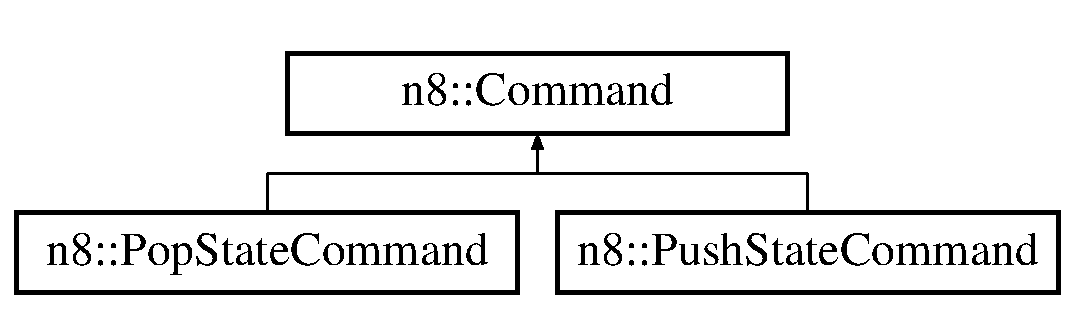
\includegraphics[height=2.000000cm]{classn8_1_1_command}
\end{center}
\end{figure}
\subsection*{Public Member Functions}
\begin{DoxyCompactItemize}
\item 
virtual \hyperlink{classn8_1_1_command_a12e333ebb6ddd65e24135b86ea31db53}{$\sim$\-Command} ()
\item 
virtual void \hyperlink{classn8_1_1_command_a8a70ef93c997ef2f545154e1c55cdf87}{execute} ()=0
\end{DoxyCompactItemize}


\subsection{Constructor \& Destructor Documentation}
\hypertarget{classn8_1_1_command_a12e333ebb6ddd65e24135b86ea31db53}{\index{n8\-::\-Command@{n8\-::\-Command}!$\sim$\-Command@{$\sim$\-Command}}
\index{$\sim$\-Command@{$\sim$\-Command}!n8::Command@{n8\-::\-Command}}
\subsubsection[{$\sim$\-Command}]{\setlength{\rightskip}{0pt plus 5cm}virtual n8\-::\-Command\-::$\sim$\-Command (
\begin{DoxyParamCaption}
{}
\end{DoxyParamCaption}
)\hspace{0.3cm}{\ttfamily [inline]}, {\ttfamily [virtual]}}}\label{classn8_1_1_command_a12e333ebb6ddd65e24135b86ea31db53}


\subsection{Member Function Documentation}
\hypertarget{classn8_1_1_command_a8a70ef93c997ef2f545154e1c55cdf87}{\index{n8\-::\-Command@{n8\-::\-Command}!execute@{execute}}
\index{execute@{execute}!n8::Command@{n8\-::\-Command}}
\subsubsection[{execute}]{\setlength{\rightskip}{0pt plus 5cm}virtual void n8\-::\-Command\-::execute (
\begin{DoxyParamCaption}
{}
\end{DoxyParamCaption}
)\hspace{0.3cm}{\ttfamily [pure virtual]}}}\label{classn8_1_1_command_a8a70ef93c997ef2f545154e1c55cdf87}


Implemented in \hyperlink{classn8_1_1_push_state_command_ab3019fecfe1aee633c6d3b3cf68f2e70}{n8\-::\-Push\-State\-Command}, and \hyperlink{classn8_1_1_pop_state_command_aa17a7fa17704fe0ba20dcebde250e19b}{n8\-::\-Pop\-State\-Command}.



The documentation for this class was generated from the following file\-:\begin{DoxyCompactItemize}
\item 
Base/\hyperlink{_command_8h}{Command.\-h}\end{DoxyCompactItemize}

\hypertarget{classtinyxml2_1_1_dyn_array}{\section{tinyxml2\-:\-:Dyn\-Array$<$ T, I\-N\-I\-T $>$ Class Template Reference}
\label{classtinyxml2_1_1_dyn_array}\index{tinyxml2\-::\-Dyn\-Array$<$ T, I\-N\-I\-T $>$@{tinyxml2\-::\-Dyn\-Array$<$ T, I\-N\-I\-T $>$}}
}


{\ttfamily \#include $<$tinyxml2.\-h$>$}

\subsection*{Public Member Functions}
\begin{DoxyCompactItemize}
\item 
\hyperlink{classtinyxml2_1_1_dyn_array_af076df9203a7eda3f3501a0c84dbbb8a}{Dyn\-Array} ()
\item 
\hyperlink{classtinyxml2_1_1_dyn_array_ac7c2dc82db9010d09041ea6bfd921fdc}{$\sim$\-Dyn\-Array} ()
\item 
void \hyperlink{classtinyxml2_1_1_dyn_array_a9c3bb53e7091804924639bb6690d763d}{Clear} ()
\item 
void \hyperlink{classtinyxml2_1_1_dyn_array_a498de53808ba0151fef54ea10bf51050}{Push} (T t)
\item 
T $\ast$ \hyperlink{classtinyxml2_1_1_dyn_array_aa3c360d40addc3b05121da9f60a01b4d}{Push\-Arr} (int count)
\item 
T \hyperlink{classtinyxml2_1_1_dyn_array_a2281e3342bc235bf391a67e362c75866}{Pop} ()
\item 
void \hyperlink{classtinyxml2_1_1_dyn_array_ab45c0836d8c0260a5b9eda7da80de71c}{Pop\-Arr} (int count)
\item 
bool \hyperlink{classtinyxml2_1_1_dyn_array_a080dc4dc68713964bb17745d4c833158}{Empty} () const 
\item 
T \& \hyperlink{classtinyxml2_1_1_dyn_array_a775a6ab4d41f0eb15bdd863d408dd58f}{operator\mbox{[}$\,$\mbox{]}} (int i)
\item 
const T \& \hyperlink{classtinyxml2_1_1_dyn_array_a1f4874c2608cbd68be1627fca9efd820}{operator\mbox{[}$\,$\mbox{]}} (int i) const 
\item 
const T \& \hyperlink{classtinyxml2_1_1_dyn_array_a9c2282ea8901b5a92ccaac2e6166a788}{Peek\-Top} () const 
\item 
int \hyperlink{classtinyxml2_1_1_dyn_array_a1299b257b62ea6b4983c488867f219b0}{Size} () const 
\item 
int \hyperlink{classtinyxml2_1_1_dyn_array_a8edbe90ed53b2e46b1b5cf53b261e4e7}{Capacity} () const 
\item 
const T $\ast$ \hyperlink{classtinyxml2_1_1_dyn_array_a1f39330daeb97d3d1dc3fc12dcf7ac67}{Mem} () const 
\item 
T $\ast$ \hyperlink{classtinyxml2_1_1_dyn_array_a0e0d60b399d54fad5b33d5008bc59c8e}{Mem} ()
\end{DoxyCompactItemize}
\subsection*{Private Member Functions}
\begin{DoxyCompactItemize}
\item 
void \hyperlink{classtinyxml2_1_1_dyn_array_a60c1143094f43766c456bee9e329cae2}{Ensure\-Capacity} (int cap)
\end{DoxyCompactItemize}
\subsection*{Private Attributes}
\begin{DoxyCompactItemize}
\item 
T $\ast$ \hyperlink{classtinyxml2_1_1_dyn_array_a2fe3376b05543f93edf3ba1bc4947e6d}{\-\_\-mem}
\item 
T \hyperlink{classtinyxml2_1_1_dyn_array_ac00ff7104e1f9eb7a6d2e6f410cd7c12}{\-\_\-pool} \mbox{[}I\-N\-I\-T\mbox{]}
\item 
int \hyperlink{classtinyxml2_1_1_dyn_array_a9bcaa041ce3fcd254328200debebc979}{\-\_\-allocated}
\item 
int \hyperlink{classtinyxml2_1_1_dyn_array_a7177b0ed99f814eb04be4388f1f4320f}{\-\_\-size}
\end{DoxyCompactItemize}


\subsection{Constructor \& Destructor Documentation}
\hypertarget{classtinyxml2_1_1_dyn_array_af076df9203a7eda3f3501a0c84dbbb8a}{\index{tinyxml2\-::\-Dyn\-Array@{tinyxml2\-::\-Dyn\-Array}!Dyn\-Array@{Dyn\-Array}}
\index{Dyn\-Array@{Dyn\-Array}!tinyxml2::DynArray@{tinyxml2\-::\-Dyn\-Array}}
\subsubsection[{Dyn\-Array}]{\setlength{\rightskip}{0pt plus 5cm}template$<$class T, int I\-N\-I\-T$>$ {\bf tinyxml2\-::\-Dyn\-Array}$<$ T, I\-N\-I\-T $>$\-::{\bf Dyn\-Array} (
\begin{DoxyParamCaption}
{}
\end{DoxyParamCaption}
)\hspace{0.3cm}{\ttfamily [inline]}}}\label{classtinyxml2_1_1_dyn_array_af076df9203a7eda3f3501a0c84dbbb8a}
\hypertarget{classtinyxml2_1_1_dyn_array_ac7c2dc82db9010d09041ea6bfd921fdc}{\index{tinyxml2\-::\-Dyn\-Array@{tinyxml2\-::\-Dyn\-Array}!$\sim$\-Dyn\-Array@{$\sim$\-Dyn\-Array}}
\index{$\sim$\-Dyn\-Array@{$\sim$\-Dyn\-Array}!tinyxml2::DynArray@{tinyxml2\-::\-Dyn\-Array}}
\subsubsection[{$\sim$\-Dyn\-Array}]{\setlength{\rightskip}{0pt plus 5cm}template$<$class T, int I\-N\-I\-T$>$ {\bf tinyxml2\-::\-Dyn\-Array}$<$ T, I\-N\-I\-T $>$\-::$\sim${\bf Dyn\-Array} (
\begin{DoxyParamCaption}
{}
\end{DoxyParamCaption}
)\hspace{0.3cm}{\ttfamily [inline]}}}\label{classtinyxml2_1_1_dyn_array_ac7c2dc82db9010d09041ea6bfd921fdc}


\subsection{Member Function Documentation}
\hypertarget{classtinyxml2_1_1_dyn_array_a8edbe90ed53b2e46b1b5cf53b261e4e7}{\index{tinyxml2\-::\-Dyn\-Array@{tinyxml2\-::\-Dyn\-Array}!Capacity@{Capacity}}
\index{Capacity@{Capacity}!tinyxml2::DynArray@{tinyxml2\-::\-Dyn\-Array}}
\subsubsection[{Capacity}]{\setlength{\rightskip}{0pt plus 5cm}template$<$class T, int I\-N\-I\-T$>$ int {\bf tinyxml2\-::\-Dyn\-Array}$<$ T, I\-N\-I\-T $>$\-::Capacity (
\begin{DoxyParamCaption}
{}
\end{DoxyParamCaption}
) const\hspace{0.3cm}{\ttfamily [inline]}}}\label{classtinyxml2_1_1_dyn_array_a8edbe90ed53b2e46b1b5cf53b261e4e7}
\hypertarget{classtinyxml2_1_1_dyn_array_a9c3bb53e7091804924639bb6690d763d}{\index{tinyxml2\-::\-Dyn\-Array@{tinyxml2\-::\-Dyn\-Array}!Clear@{Clear}}
\index{Clear@{Clear}!tinyxml2::DynArray@{tinyxml2\-::\-Dyn\-Array}}
\subsubsection[{Clear}]{\setlength{\rightskip}{0pt plus 5cm}template$<$class T, int I\-N\-I\-T$>$ void {\bf tinyxml2\-::\-Dyn\-Array}$<$ T, I\-N\-I\-T $>$\-::Clear (
\begin{DoxyParamCaption}
{}
\end{DoxyParamCaption}
)\hspace{0.3cm}{\ttfamily [inline]}}}\label{classtinyxml2_1_1_dyn_array_a9c3bb53e7091804924639bb6690d763d}
\hypertarget{classtinyxml2_1_1_dyn_array_a080dc4dc68713964bb17745d4c833158}{\index{tinyxml2\-::\-Dyn\-Array@{tinyxml2\-::\-Dyn\-Array}!Empty@{Empty}}
\index{Empty@{Empty}!tinyxml2::DynArray@{tinyxml2\-::\-Dyn\-Array}}
\subsubsection[{Empty}]{\setlength{\rightskip}{0pt plus 5cm}template$<$class T, int I\-N\-I\-T$>$ bool {\bf tinyxml2\-::\-Dyn\-Array}$<$ T, I\-N\-I\-T $>$\-::Empty (
\begin{DoxyParamCaption}
{}
\end{DoxyParamCaption}
) const\hspace{0.3cm}{\ttfamily [inline]}}}\label{classtinyxml2_1_1_dyn_array_a080dc4dc68713964bb17745d4c833158}
\hypertarget{classtinyxml2_1_1_dyn_array_a60c1143094f43766c456bee9e329cae2}{\index{tinyxml2\-::\-Dyn\-Array@{tinyxml2\-::\-Dyn\-Array}!Ensure\-Capacity@{Ensure\-Capacity}}
\index{Ensure\-Capacity@{Ensure\-Capacity}!tinyxml2::DynArray@{tinyxml2\-::\-Dyn\-Array}}
\subsubsection[{Ensure\-Capacity}]{\setlength{\rightskip}{0pt plus 5cm}template$<$class T, int I\-N\-I\-T$>$ void {\bf tinyxml2\-::\-Dyn\-Array}$<$ T, I\-N\-I\-T $>$\-::Ensure\-Capacity (
\begin{DoxyParamCaption}
\item[{int}]{cap}
\end{DoxyParamCaption}
)\hspace{0.3cm}{\ttfamily [inline]}, {\ttfamily [private]}}}\label{classtinyxml2_1_1_dyn_array_a60c1143094f43766c456bee9e329cae2}
\hypertarget{classtinyxml2_1_1_dyn_array_a1f39330daeb97d3d1dc3fc12dcf7ac67}{\index{tinyxml2\-::\-Dyn\-Array@{tinyxml2\-::\-Dyn\-Array}!Mem@{Mem}}
\index{Mem@{Mem}!tinyxml2::DynArray@{tinyxml2\-::\-Dyn\-Array}}
\subsubsection[{Mem}]{\setlength{\rightskip}{0pt plus 5cm}template$<$class T, int I\-N\-I\-T$>$ const T$\ast$ {\bf tinyxml2\-::\-Dyn\-Array}$<$ T, I\-N\-I\-T $>$\-::Mem (
\begin{DoxyParamCaption}
{}
\end{DoxyParamCaption}
) const\hspace{0.3cm}{\ttfamily [inline]}}}\label{classtinyxml2_1_1_dyn_array_a1f39330daeb97d3d1dc3fc12dcf7ac67}
\hypertarget{classtinyxml2_1_1_dyn_array_a0e0d60b399d54fad5b33d5008bc59c8e}{\index{tinyxml2\-::\-Dyn\-Array@{tinyxml2\-::\-Dyn\-Array}!Mem@{Mem}}
\index{Mem@{Mem}!tinyxml2::DynArray@{tinyxml2\-::\-Dyn\-Array}}
\subsubsection[{Mem}]{\setlength{\rightskip}{0pt plus 5cm}template$<$class T, int I\-N\-I\-T$>$ T$\ast$ {\bf tinyxml2\-::\-Dyn\-Array}$<$ T, I\-N\-I\-T $>$\-::Mem (
\begin{DoxyParamCaption}
{}
\end{DoxyParamCaption}
)\hspace{0.3cm}{\ttfamily [inline]}}}\label{classtinyxml2_1_1_dyn_array_a0e0d60b399d54fad5b33d5008bc59c8e}
\hypertarget{classtinyxml2_1_1_dyn_array_a775a6ab4d41f0eb15bdd863d408dd58f}{\index{tinyxml2\-::\-Dyn\-Array@{tinyxml2\-::\-Dyn\-Array}!operator\mbox{[}$\,$\mbox{]}@{operator[]}}
\index{operator\mbox{[}$\,$\mbox{]}@{operator[]}!tinyxml2::DynArray@{tinyxml2\-::\-Dyn\-Array}}
\subsubsection[{operator[]}]{\setlength{\rightskip}{0pt plus 5cm}template$<$class T, int I\-N\-I\-T$>$ T\& {\bf tinyxml2\-::\-Dyn\-Array}$<$ T, I\-N\-I\-T $>$\-::operator\mbox{[}$\,$\mbox{]} (
\begin{DoxyParamCaption}
\item[{int}]{i}
\end{DoxyParamCaption}
)\hspace{0.3cm}{\ttfamily [inline]}}}\label{classtinyxml2_1_1_dyn_array_a775a6ab4d41f0eb15bdd863d408dd58f}
\hypertarget{classtinyxml2_1_1_dyn_array_a1f4874c2608cbd68be1627fca9efd820}{\index{tinyxml2\-::\-Dyn\-Array@{tinyxml2\-::\-Dyn\-Array}!operator\mbox{[}$\,$\mbox{]}@{operator[]}}
\index{operator\mbox{[}$\,$\mbox{]}@{operator[]}!tinyxml2::DynArray@{tinyxml2\-::\-Dyn\-Array}}
\subsubsection[{operator[]}]{\setlength{\rightskip}{0pt plus 5cm}template$<$class T, int I\-N\-I\-T$>$ const T\& {\bf tinyxml2\-::\-Dyn\-Array}$<$ T, I\-N\-I\-T $>$\-::operator\mbox{[}$\,$\mbox{]} (
\begin{DoxyParamCaption}
\item[{int}]{i}
\end{DoxyParamCaption}
) const\hspace{0.3cm}{\ttfamily [inline]}}}\label{classtinyxml2_1_1_dyn_array_a1f4874c2608cbd68be1627fca9efd820}
\hypertarget{classtinyxml2_1_1_dyn_array_a9c2282ea8901b5a92ccaac2e6166a788}{\index{tinyxml2\-::\-Dyn\-Array@{tinyxml2\-::\-Dyn\-Array}!Peek\-Top@{Peek\-Top}}
\index{Peek\-Top@{Peek\-Top}!tinyxml2::DynArray@{tinyxml2\-::\-Dyn\-Array}}
\subsubsection[{Peek\-Top}]{\setlength{\rightskip}{0pt plus 5cm}template$<$class T, int I\-N\-I\-T$>$ const T\& {\bf tinyxml2\-::\-Dyn\-Array}$<$ T, I\-N\-I\-T $>$\-::Peek\-Top (
\begin{DoxyParamCaption}
{}
\end{DoxyParamCaption}
) const\hspace{0.3cm}{\ttfamily [inline]}}}\label{classtinyxml2_1_1_dyn_array_a9c2282ea8901b5a92ccaac2e6166a788}
\hypertarget{classtinyxml2_1_1_dyn_array_a2281e3342bc235bf391a67e362c75866}{\index{tinyxml2\-::\-Dyn\-Array@{tinyxml2\-::\-Dyn\-Array}!Pop@{Pop}}
\index{Pop@{Pop}!tinyxml2::DynArray@{tinyxml2\-::\-Dyn\-Array}}
\subsubsection[{Pop}]{\setlength{\rightskip}{0pt plus 5cm}template$<$class T, int I\-N\-I\-T$>$ T {\bf tinyxml2\-::\-Dyn\-Array}$<$ T, I\-N\-I\-T $>$\-::Pop (
\begin{DoxyParamCaption}
{}
\end{DoxyParamCaption}
)\hspace{0.3cm}{\ttfamily [inline]}}}\label{classtinyxml2_1_1_dyn_array_a2281e3342bc235bf391a67e362c75866}
\hypertarget{classtinyxml2_1_1_dyn_array_ab45c0836d8c0260a5b9eda7da80de71c}{\index{tinyxml2\-::\-Dyn\-Array@{tinyxml2\-::\-Dyn\-Array}!Pop\-Arr@{Pop\-Arr}}
\index{Pop\-Arr@{Pop\-Arr}!tinyxml2::DynArray@{tinyxml2\-::\-Dyn\-Array}}
\subsubsection[{Pop\-Arr}]{\setlength{\rightskip}{0pt plus 5cm}template$<$class T, int I\-N\-I\-T$>$ void {\bf tinyxml2\-::\-Dyn\-Array}$<$ T, I\-N\-I\-T $>$\-::Pop\-Arr (
\begin{DoxyParamCaption}
\item[{int}]{count}
\end{DoxyParamCaption}
)\hspace{0.3cm}{\ttfamily [inline]}}}\label{classtinyxml2_1_1_dyn_array_ab45c0836d8c0260a5b9eda7da80de71c}
\hypertarget{classtinyxml2_1_1_dyn_array_a498de53808ba0151fef54ea10bf51050}{\index{tinyxml2\-::\-Dyn\-Array@{tinyxml2\-::\-Dyn\-Array}!Push@{Push}}
\index{Push@{Push}!tinyxml2::DynArray@{tinyxml2\-::\-Dyn\-Array}}
\subsubsection[{Push}]{\setlength{\rightskip}{0pt plus 5cm}template$<$class T, int I\-N\-I\-T$>$ void {\bf tinyxml2\-::\-Dyn\-Array}$<$ T, I\-N\-I\-T $>$\-::Push (
\begin{DoxyParamCaption}
\item[{T}]{t}
\end{DoxyParamCaption}
)\hspace{0.3cm}{\ttfamily [inline]}}}\label{classtinyxml2_1_1_dyn_array_a498de53808ba0151fef54ea10bf51050}
\hypertarget{classtinyxml2_1_1_dyn_array_aa3c360d40addc3b05121da9f60a01b4d}{\index{tinyxml2\-::\-Dyn\-Array@{tinyxml2\-::\-Dyn\-Array}!Push\-Arr@{Push\-Arr}}
\index{Push\-Arr@{Push\-Arr}!tinyxml2::DynArray@{tinyxml2\-::\-Dyn\-Array}}
\subsubsection[{Push\-Arr}]{\setlength{\rightskip}{0pt plus 5cm}template$<$class T, int I\-N\-I\-T$>$ T$\ast$ {\bf tinyxml2\-::\-Dyn\-Array}$<$ T, I\-N\-I\-T $>$\-::Push\-Arr (
\begin{DoxyParamCaption}
\item[{int}]{count}
\end{DoxyParamCaption}
)\hspace{0.3cm}{\ttfamily [inline]}}}\label{classtinyxml2_1_1_dyn_array_aa3c360d40addc3b05121da9f60a01b4d}
\hypertarget{classtinyxml2_1_1_dyn_array_a1299b257b62ea6b4983c488867f219b0}{\index{tinyxml2\-::\-Dyn\-Array@{tinyxml2\-::\-Dyn\-Array}!Size@{Size}}
\index{Size@{Size}!tinyxml2::DynArray@{tinyxml2\-::\-Dyn\-Array}}
\subsubsection[{Size}]{\setlength{\rightskip}{0pt plus 5cm}template$<$class T, int I\-N\-I\-T$>$ int {\bf tinyxml2\-::\-Dyn\-Array}$<$ T, I\-N\-I\-T $>$\-::Size (
\begin{DoxyParamCaption}
{}
\end{DoxyParamCaption}
) const\hspace{0.3cm}{\ttfamily [inline]}}}\label{classtinyxml2_1_1_dyn_array_a1299b257b62ea6b4983c488867f219b0}


\subsection{Member Data Documentation}
\hypertarget{classtinyxml2_1_1_dyn_array_a9bcaa041ce3fcd254328200debebc979}{\index{tinyxml2\-::\-Dyn\-Array@{tinyxml2\-::\-Dyn\-Array}!\-\_\-allocated@{\-\_\-allocated}}
\index{\-\_\-allocated@{\-\_\-allocated}!tinyxml2::DynArray@{tinyxml2\-::\-Dyn\-Array}}
\subsubsection[{\-\_\-allocated}]{\setlength{\rightskip}{0pt plus 5cm}template$<$class T, int I\-N\-I\-T$>$ int {\bf tinyxml2\-::\-Dyn\-Array}$<$ T, I\-N\-I\-T $>$\-::\-\_\-allocated\hspace{0.3cm}{\ttfamily [private]}}}\label{classtinyxml2_1_1_dyn_array_a9bcaa041ce3fcd254328200debebc979}
\hypertarget{classtinyxml2_1_1_dyn_array_a2fe3376b05543f93edf3ba1bc4947e6d}{\index{tinyxml2\-::\-Dyn\-Array@{tinyxml2\-::\-Dyn\-Array}!\-\_\-mem@{\-\_\-mem}}
\index{\-\_\-mem@{\-\_\-mem}!tinyxml2::DynArray@{tinyxml2\-::\-Dyn\-Array}}
\subsubsection[{\-\_\-mem}]{\setlength{\rightskip}{0pt plus 5cm}template$<$class T, int I\-N\-I\-T$>$ T$\ast$ {\bf tinyxml2\-::\-Dyn\-Array}$<$ T, I\-N\-I\-T $>$\-::\-\_\-mem\hspace{0.3cm}{\ttfamily [private]}}}\label{classtinyxml2_1_1_dyn_array_a2fe3376b05543f93edf3ba1bc4947e6d}
\hypertarget{classtinyxml2_1_1_dyn_array_ac00ff7104e1f9eb7a6d2e6f410cd7c12}{\index{tinyxml2\-::\-Dyn\-Array@{tinyxml2\-::\-Dyn\-Array}!\-\_\-pool@{\-\_\-pool}}
\index{\-\_\-pool@{\-\_\-pool}!tinyxml2::DynArray@{tinyxml2\-::\-Dyn\-Array}}
\subsubsection[{\-\_\-pool}]{\setlength{\rightskip}{0pt plus 5cm}template$<$class T, int I\-N\-I\-T$>$ T {\bf tinyxml2\-::\-Dyn\-Array}$<$ T, I\-N\-I\-T $>$\-::\-\_\-pool\mbox{[}I\-N\-I\-T\mbox{]}\hspace{0.3cm}{\ttfamily [private]}}}\label{classtinyxml2_1_1_dyn_array_ac00ff7104e1f9eb7a6d2e6f410cd7c12}
\hypertarget{classtinyxml2_1_1_dyn_array_a7177b0ed99f814eb04be4388f1f4320f}{\index{tinyxml2\-::\-Dyn\-Array@{tinyxml2\-::\-Dyn\-Array}!\-\_\-size@{\-\_\-size}}
\index{\-\_\-size@{\-\_\-size}!tinyxml2::DynArray@{tinyxml2\-::\-Dyn\-Array}}
\subsubsection[{\-\_\-size}]{\setlength{\rightskip}{0pt plus 5cm}template$<$class T, int I\-N\-I\-T$>$ int {\bf tinyxml2\-::\-Dyn\-Array}$<$ T, I\-N\-I\-T $>$\-::\-\_\-size\hspace{0.3cm}{\ttfamily [private]}}}\label{classtinyxml2_1_1_dyn_array_a7177b0ed99f814eb04be4388f1f4320f}


The documentation for this class was generated from the following file\-:\begin{DoxyCompactItemize}
\item 
Utils/\-X\-M\-L\-\_\-\-Config/\hyperlink{tinyxml2_8h}{tinyxml2.\-h}\end{DoxyCompactItemize}

\hypertarget{structtinyxml2_1_1_entity}{\section{tinyxml2\-:\-:Entity Struct Reference}
\label{structtinyxml2_1_1_entity}\index{tinyxml2\-::\-Entity@{tinyxml2\-::\-Entity}}
}
\subsection*{Public Attributes}
\begin{DoxyCompactItemize}
\item 
const char $\ast$ \hyperlink{structtinyxml2_1_1_entity_ab330f5d665d29bfc811ecfa76315894b}{pattern}
\item 
int \hyperlink{structtinyxml2_1_1_entity_a25e2b57cb59cb4fa68f283d7cb570f21}{length}
\item 
char \hyperlink{structtinyxml2_1_1_entity_a7334e81e33b4615655a403711b24f3ed}{value}
\end{DoxyCompactItemize}


\subsection{Member Data Documentation}
\hypertarget{structtinyxml2_1_1_entity_a25e2b57cb59cb4fa68f283d7cb570f21}{\index{tinyxml2\-::\-Entity@{tinyxml2\-::\-Entity}!length@{length}}
\index{length@{length}!tinyxml2::Entity@{tinyxml2\-::\-Entity}}
\subsubsection[{length}]{\setlength{\rightskip}{0pt plus 5cm}int tinyxml2\-::\-Entity\-::length}}\label{structtinyxml2_1_1_entity_a25e2b57cb59cb4fa68f283d7cb570f21}
\hypertarget{structtinyxml2_1_1_entity_ab330f5d665d29bfc811ecfa76315894b}{\index{tinyxml2\-::\-Entity@{tinyxml2\-::\-Entity}!pattern@{pattern}}
\index{pattern@{pattern}!tinyxml2::Entity@{tinyxml2\-::\-Entity}}
\subsubsection[{pattern}]{\setlength{\rightskip}{0pt plus 5cm}const char$\ast$ tinyxml2\-::\-Entity\-::pattern}}\label{structtinyxml2_1_1_entity_ab330f5d665d29bfc811ecfa76315894b}
\hypertarget{structtinyxml2_1_1_entity_a7334e81e33b4615655a403711b24f3ed}{\index{tinyxml2\-::\-Entity@{tinyxml2\-::\-Entity}!value@{value}}
\index{value@{value}!tinyxml2::Entity@{tinyxml2\-::\-Entity}}
\subsubsection[{value}]{\setlength{\rightskip}{0pt plus 5cm}char tinyxml2\-::\-Entity\-::value}}\label{structtinyxml2_1_1_entity_a7334e81e33b4615655a403711b24f3ed}


The documentation for this struct was generated from the following file\-:\begin{DoxyCompactItemize}
\item 
Utils/\-X\-M\-L\-\_\-\-Config/\hyperlink{tinyxml2_8cpp}{tinyxml2.\-cpp}\end{DoxyCompactItemize}

\hypertarget{classn8_1_1_event}{\section{n8\-:\-:Event Class Reference}
\label{classn8_1_1_event}\index{n8\-::\-Event@{n8\-::\-Event}}
}


{\ttfamily \#include $<$Event.\-h$>$}

\subsection*{Public Member Functions}
\begin{DoxyCompactItemize}
\item 
\hyperlink{classn8_1_1_event_a09ae792fcd364ecb41d7ac31a1b91355}{Event} (\hyperlink{namespace_e_events_ad7951ce20842f9eeb617fae73d4c9504}{E\-Events\-::\-Values})
\item 
\hyperlink{namespace_e_events_ad7951ce20842f9eeb617fae73d4c9504}{E\-Events\-::\-Values} \hyperlink{classn8_1_1_event_a8298170bd089652972f44c92d6c0c21d}{Get\-Type} ()
\end{DoxyCompactItemize}
\subsection*{Private Attributes}
\begin{DoxyCompactItemize}
\item 
\hyperlink{namespace_e_events_ad7951ce20842f9eeb617fae73d4c9504}{E\-Events\-::\-Values} \hyperlink{classn8_1_1_event_a6e5397ed6c7311cb8f9c84747a658cd0}{m\-\_\-type}
\end{DoxyCompactItemize}


\subsection{Detailed Description}
Class to pass events between observable systems 

\subsection{Constructor \& Destructor Documentation}
\hypertarget{classn8_1_1_event_a09ae792fcd364ecb41d7ac31a1b91355}{\index{n8\-::\-Event@{n8\-::\-Event}!Event@{Event}}
\index{Event@{Event}!n8::Event@{n8\-::\-Event}}
\subsubsection[{Event}]{\setlength{\rightskip}{0pt plus 5cm}n8\-::\-Event\-::\-Event (
\begin{DoxyParamCaption}
\item[{{\bf E\-Events\-::\-Values}}]{type}
\end{DoxyParamCaption}
)}}\label{classn8_1_1_event_a09ae792fcd364ecb41d7ac31a1b91355}
Constructor Creates the event and sets its type


\begin{DoxyParams}{Parameters}
{\em type} & The type of the event \\
\hline
\end{DoxyParams}


\subsection{Member Function Documentation}
\hypertarget{classn8_1_1_event_a8298170bd089652972f44c92d6c0c21d}{\index{n8\-::\-Event@{n8\-::\-Event}!Get\-Type@{Get\-Type}}
\index{Get\-Type@{Get\-Type}!n8::Event@{n8\-::\-Event}}
\subsubsection[{Get\-Type}]{\setlength{\rightskip}{0pt plus 5cm}{\bf E\-Events\-::\-Values} n8\-::\-Event\-::\-Get\-Type (
\begin{DoxyParamCaption}
{}
\end{DoxyParamCaption}
)}}\label{classn8_1_1_event_a8298170bd089652972f44c92d6c0c21d}
Get\-Type Used to get the type of an event so it can be properly handled

\begin{DoxyReturn}{Returns}
The type of the event 
\end{DoxyReturn}


\subsection{Member Data Documentation}
\hypertarget{classn8_1_1_event_a6e5397ed6c7311cb8f9c84747a658cd0}{\index{n8\-::\-Event@{n8\-::\-Event}!m\-\_\-type@{m\-\_\-type}}
\index{m\-\_\-type@{m\-\_\-type}!n8::Event@{n8\-::\-Event}}
\subsubsection[{m\-\_\-type}]{\setlength{\rightskip}{0pt plus 5cm}{\bf E\-Events\-::\-Values} n8\-::\-Event\-::m\-\_\-type\hspace{0.3cm}{\ttfamily [private]}}}\label{classn8_1_1_event_a6e5397ed6c7311cb8f9c84747a658cd0}


The documentation for this class was generated from the following files\-:\begin{DoxyCompactItemize}
\item 
Communication/\hyperlink{_event_8h}{Event.\-h}\item 
Communication/\hyperlink{_event_8cpp}{Event.\-cpp}\end{DoxyCompactItemize}

\hypertarget{classn8_1_1_font}{\section{n8\-:\-:Font Class Reference}
\label{classn8_1_1_font}\index{n8\-::\-Font@{n8\-::\-Font}}
}


{\ttfamily \#include $<$Font.\-h$>$}

Inheritance diagram for n8\-:\-:Font\-:\begin{figure}[H]
\begin{center}
\leavevmode
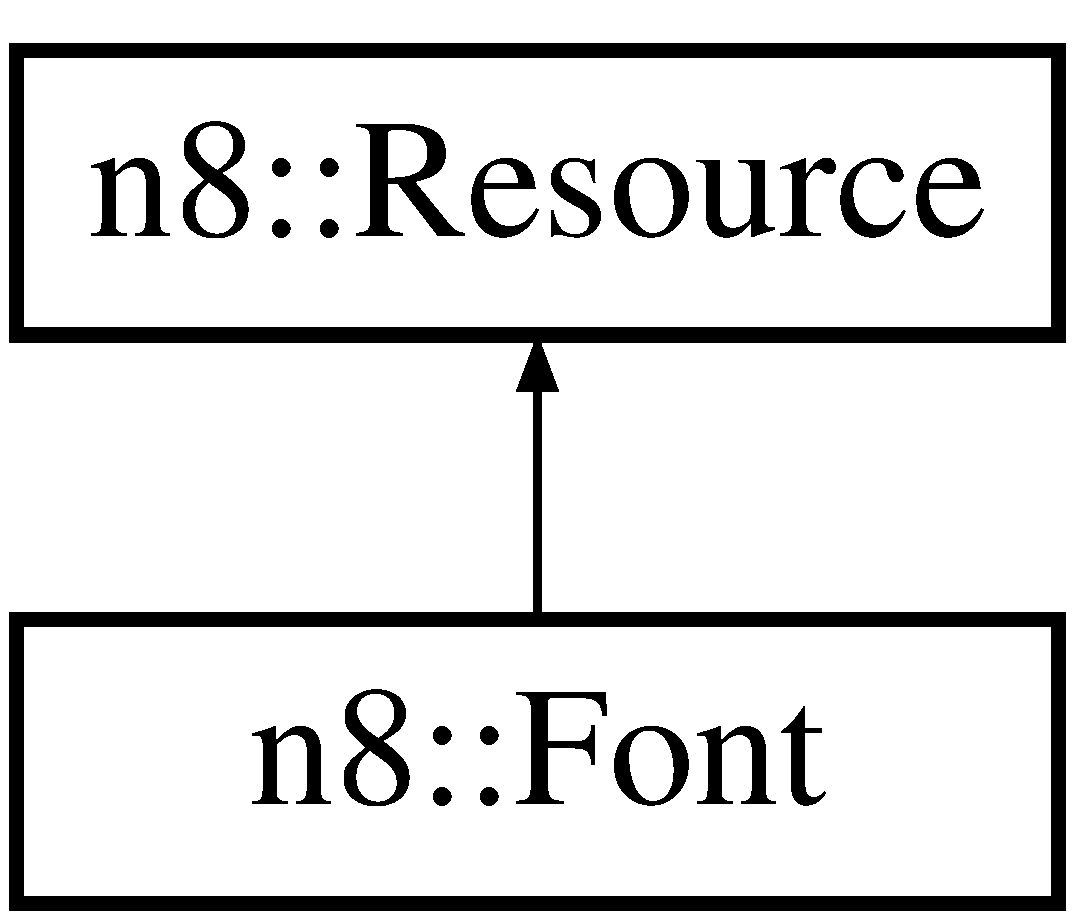
\includegraphics[height=2.000000cm]{classn8_1_1_font}
\end{center}
\end{figure}
\subsection*{Public Member Functions}
\begin{DoxyCompactItemize}
\item 
\hyperlink{classn8_1_1_font_ae8b9fc4f6c39d58dc0024dcf2b6e2cd1}{Font} (std\-::string p\-\_\-id, T\-T\-F\-\_\-\-Font $\ast$p\-\_\-ttf\-Font)
\item 
\hyperlink{classn8_1_1_font_a147906bb47587fadfa559b187d71ff32}{$\sim$\-Font} ()
\end{DoxyCompactItemize}
\subsection*{Private Attributes}
\begin{DoxyCompactItemize}
\item 
T\-T\-F\-\_\-\-Font $\ast$ \hyperlink{classn8_1_1_font_a4f366d0c324efb7daa5deadd187bb290}{p\-\_\-font}
\end{DoxyCompactItemize}
\subsection*{Friends}
\begin{DoxyCompactItemize}
\item 
class \hyperlink{classn8_1_1_font_aedde775898ebe0d7c84c0060e1c9d770}{Render\-Service}
\end{DoxyCompactItemize}


\subsection{Constructor \& Destructor Documentation}
\hypertarget{classn8_1_1_font_ae8b9fc4f6c39d58dc0024dcf2b6e2cd1}{\index{n8\-::\-Font@{n8\-::\-Font}!Font@{Font}}
\index{Font@{Font}!n8::Font@{n8\-::\-Font}}
\subsubsection[{Font}]{\setlength{\rightskip}{0pt plus 5cm}n8\-::\-Font\-::\-Font (
\begin{DoxyParamCaption}
\item[{std\-::string}]{p\-\_\-id, }
\item[{T\-T\-F\-\_\-\-Font $\ast$}]{p\-\_\-ttf\-Font}
\end{DoxyParamCaption}
)}}\label{classn8_1_1_font_ae8b9fc4f6c39d58dc0024dcf2b6e2cd1}
\hypertarget{classn8_1_1_font_a147906bb47587fadfa559b187d71ff32}{\index{n8\-::\-Font@{n8\-::\-Font}!$\sim$\-Font@{$\sim$\-Font}}
\index{$\sim$\-Font@{$\sim$\-Font}!n8::Font@{n8\-::\-Font}}
\subsubsection[{$\sim$\-Font}]{\setlength{\rightskip}{0pt plus 5cm}n8\-::\-Font\-::$\sim$\-Font (
\begin{DoxyParamCaption}
{}
\end{DoxyParamCaption}
)}}\label{classn8_1_1_font_a147906bb47587fadfa559b187d71ff32}


\subsection{Friends And Related Function Documentation}
\hypertarget{classn8_1_1_font_aedde775898ebe0d7c84c0060e1c9d770}{\index{n8\-::\-Font@{n8\-::\-Font}!Render\-Service@{Render\-Service}}
\index{Render\-Service@{Render\-Service}!n8::Font@{n8\-::\-Font}}
\subsubsection[{Render\-Service}]{\setlength{\rightskip}{0pt plus 5cm}friend class Render\-Service\hspace{0.3cm}{\ttfamily [friend]}}}\label{classn8_1_1_font_aedde775898ebe0d7c84c0060e1c9d770}


\subsection{Member Data Documentation}
\hypertarget{classn8_1_1_font_a4f366d0c324efb7daa5deadd187bb290}{\index{n8\-::\-Font@{n8\-::\-Font}!p\-\_\-font@{p\-\_\-font}}
\index{p\-\_\-font@{p\-\_\-font}!n8::Font@{n8\-::\-Font}}
\subsubsection[{p\-\_\-font}]{\setlength{\rightskip}{0pt plus 5cm}T\-T\-F\-\_\-\-Font$\ast$ n8\-::\-Font\-::p\-\_\-font\hspace{0.3cm}{\ttfamily [private]}}}\label{classn8_1_1_font_a4f366d0c324efb7daa5deadd187bb290}


The documentation for this class was generated from the following files\-:\begin{DoxyCompactItemize}
\item 
Resources/\hyperlink{_font_8h}{Font.\-h}\item 
Resources/\hyperlink{_font_8cpp}{Font.\-cpp}\end{DoxyCompactItemize}

\hypertarget{classn8_1_1_game}{\section{n8\-:\-:Game Class Reference}
\label{classn8_1_1_game}\index{n8\-::\-Game@{n8\-::\-Game}}
}


{\ttfamily \#include $<$Game.\-h$>$}

\subsection*{Public Member Functions}
\begin{DoxyCompactItemize}
\item 
\hyperlink{classn8_1_1_game_a53a0ff7f30b16f7f6ba3c564d3bb2500}{Game} (const char $\ast$)
\item 
\hyperlink{classn8_1_1_game_a66c22b00c1ba720ad07f2a69da52932b}{$\sim$\-Game} ()
\item 
void \hyperlink{classn8_1_1_game_a364cbd476cf05de2b01310d4019afeb1}{Setup} ()
\item 
void \hyperlink{classn8_1_1_game_ab9f5035750e9d603187aaa3c33f6fd07}{Start} ()
\item 
void \hyperlink{classn8_1_1_game_acf99e1b0f6e504887dc9dc9a65bab3db}{Stop} ()
\item 
void \hyperlink{classn8_1_1_game_a30ff8d65fecc1f69edb401ad7d823bbb}{Set\-F\-P\-S} (unsigned)
\item 
void \hyperlink{classn8_1_1_game_ad63ea9f9325bedcb2d4d286e734d4e62}{Define\-Window\-Size} (unsigned, unsigned)
\item 
void \hyperlink{classn8_1_1_game_ab34fca1a3d62a460a2b470c59ef77372}{Register\-State} (\hyperlink{namespace_e_state_aee586325ec9fecd1205d41439870dd81}{E\-State\-::\-Values}, \hyperlink{classn8_1_1_state}{State} $\ast$)
\item 
void \hyperlink{classn8_1_1_game_a0c046c84911b1b02aeaed2e15da487a0}{Set\-Start\-State} (\hyperlink{namespace_e_state_aee586325ec9fecd1205d41439870dd81}{E\-State\-::\-Values})
\end{DoxyCompactItemize}
\subsection*{Static Public Member Functions}
\begin{DoxyCompactItemize}
\item 
static void \hyperlink{classn8_1_1_game_a07f1d9b3613d256ed65abc029f45263b}{Init} ()
\item 
static void \hyperlink{classn8_1_1_game_a2030218945ee955cb97e9c9c5dc31b0a}{Shutdown} ()
\end{DoxyCompactItemize}
\subsection*{Static Public Attributes}
\begin{DoxyCompactItemize}
\item 
static const int \hyperlink{classn8_1_1_game_ad5b5e680104848b530623a0ff2984dd9}{D\-E\-F\-A\-U\-L\-T\-\_\-\-F\-P\-S} = 60
\end{DoxyCompactItemize}
\subsection*{Private Member Functions}
\begin{DoxyCompactItemize}
\item 
void \hyperlink{classn8_1_1_game_a3086b13e04d6926b60c25250702e0f76}{Process\-Config\-File} ()
\item 
void \hyperlink{classn8_1_1_game_a177132db60f27b7b72cedebe8b3c31ff}{Initialize\-Directory\-Path} ()
\item 
void \hyperlink{classn8_1_1_game_a406cab23a3df73bb69e29b6e6f0de5a4}{Initialize\-Resources\-Path} ()
\end{DoxyCompactItemize}
\subsection*{Private Attributes}
\begin{DoxyCompactItemize}
\item 
const std\-::string \hyperlink{classn8_1_1_game_a4ba4f2b01a5cc821bdfeb371141eb7c5}{R\-E\-S\-O\-U\-R\-C\-E\-\_\-\-F\-I\-L\-E\-\_\-\-S\-U\-F\-F\-I\-X} = \char`\"{}Resources.\-xml\char`\"{}
\item 
\hyperlink{classn8_1_1_service_manager}{Service\-Manager} $\ast$ \hyperlink{classn8_1_1_game_a30bd8276bfbc388dbade2b4c267b8475}{m\-\_\-service\-Manager}
\item 
\hyperlink{classn8_1_1_window}{n8\-::\-Window} \hyperlink{classn8_1_1_game_a091449bc88fce9f180acbcca101ebdbe}{m\-\_\-window}
\item 
\hyperlink{classn8_1_1_timer}{n8\-::\-Timer} \hyperlink{classn8_1_1_game_a0eab78b9c0f627925ffb1124d6272dff}{m\-\_\-timer}
\item 
int \hyperlink{classn8_1_1_game_a6a379dae9cb3bc1f8b423373600dd037}{m\-\_\-fps}
\item 
bool \hyperlink{classn8_1_1_game_a75f5cfb356d519dcdf9b5ef7db25006f}{m\-\_\-quit}
\item 
unsigned \hyperlink{classn8_1_1_game_ae1e6c5b939a154d09ed65496156090ec}{m\-\_\-window\-Width}
\item 
unsigned \hyperlink{classn8_1_1_game_af3e88c8758f2e09303408637cbbf656f}{m\-\_\-window\-Height}
\item 
std\-::string \hyperlink{classn8_1_1_game_a3e6ebc71d694ec81fd28e99ccc44794a}{m\-\_\-config\-Path}
\item 
std\-::string \hyperlink{classn8_1_1_game_a8c04b39e97c22b6fdf8fb1861f09c556}{m\-\_\-directory\-Path}
\item 
std\-::string \hyperlink{classn8_1_1_game_a19483f2905db0ae25cfd3b7c9efd69ef}{m\-\_\-resources\-List\-Path}
\end{DoxyCompactItemize}


\subsection{Constructor \& Destructor Documentation}
\hypertarget{classn8_1_1_game_a53a0ff7f30b16f7f6ba3c564d3bb2500}{\index{n8\-::\-Game@{n8\-::\-Game}!Game@{Game}}
\index{Game@{Game}!n8::Game@{n8\-::\-Game}}
\subsubsection[{Game}]{\setlength{\rightskip}{0pt plus 5cm}n8\-::\-Game\-::\-Game (
\begin{DoxyParamCaption}
\item[{const char $\ast$}]{config\-File}
\end{DoxyParamCaption}
)}}\label{classn8_1_1_game_a53a0ff7f30b16f7f6ba3c564d3bb2500}
Default Constructor \hypertarget{classn8_1_1_game_a66c22b00c1ba720ad07f2a69da52932b}{\index{n8\-::\-Game@{n8\-::\-Game}!$\sim$\-Game@{$\sim$\-Game}}
\index{$\sim$\-Game@{$\sim$\-Game}!n8::Game@{n8\-::\-Game}}
\subsubsection[{$\sim$\-Game}]{\setlength{\rightskip}{0pt plus 5cm}n8\-::\-Game\-::$\sim$\-Game (
\begin{DoxyParamCaption}
{}
\end{DoxyParamCaption}
)}}\label{classn8_1_1_game_a66c22b00c1ba720ad07f2a69da52932b}
Destructor 

\subsection{Member Function Documentation}
\hypertarget{classn8_1_1_game_ad63ea9f9325bedcb2d4d286e734d4e62}{\index{n8\-::\-Game@{n8\-::\-Game}!Define\-Window\-Size@{Define\-Window\-Size}}
\index{Define\-Window\-Size@{Define\-Window\-Size}!n8::Game@{n8\-::\-Game}}
\subsubsection[{Define\-Window\-Size}]{\setlength{\rightskip}{0pt plus 5cm}void n8\-::\-Game\-::\-Define\-Window\-Size (
\begin{DoxyParamCaption}
\item[{unsigned}]{width, }
\item[{unsigned}]{height}
\end{DoxyParamCaption}
)}}\label{classn8_1_1_game_ad63ea9f9325bedcb2d4d286e734d4e62}
Resize\-Window Changes the dimensions of the game window


\begin{DoxyParams}{Parameters}
{\em unsigned} & width The desired width of the window \\
\hline
{\em unsigned} & height The desired height of the window \\
\hline
\end{DoxyParams}
\hypertarget{classn8_1_1_game_a07f1d9b3613d256ed65abc029f45263b}{\index{n8\-::\-Game@{n8\-::\-Game}!Init@{Init}}
\index{Init@{Init}!n8::Game@{n8\-::\-Game}}
\subsubsection[{Init}]{\setlength{\rightskip}{0pt plus 5cm}void n8\-::\-Game\-::\-Init (
\begin{DoxyParamCaption}
{}
\end{DoxyParamCaption}
)\hspace{0.3cm}{\ttfamily [static]}}}\label{classn8_1_1_game_a07f1d9b3613d256ed65abc029f45263b}
\hypertarget{classn8_1_1_game_a177132db60f27b7b72cedebe8b3c31ff}{\index{n8\-::\-Game@{n8\-::\-Game}!Initialize\-Directory\-Path@{Initialize\-Directory\-Path}}
\index{Initialize\-Directory\-Path@{Initialize\-Directory\-Path}!n8::Game@{n8\-::\-Game}}
\subsubsection[{Initialize\-Directory\-Path}]{\setlength{\rightskip}{0pt plus 5cm}void n8\-::\-Game\-::\-Initialize\-Directory\-Path (
\begin{DoxyParamCaption}
{}
\end{DoxyParamCaption}
)\hspace{0.3cm}{\ttfamily [private]}}}\label{classn8_1_1_game_a177132db60f27b7b72cedebe8b3c31ff}
\hypertarget{classn8_1_1_game_a406cab23a3df73bb69e29b6e6f0de5a4}{\index{n8\-::\-Game@{n8\-::\-Game}!Initialize\-Resources\-Path@{Initialize\-Resources\-Path}}
\index{Initialize\-Resources\-Path@{Initialize\-Resources\-Path}!n8::Game@{n8\-::\-Game}}
\subsubsection[{Initialize\-Resources\-Path}]{\setlength{\rightskip}{0pt plus 5cm}void n8\-::\-Game\-::\-Initialize\-Resources\-Path (
\begin{DoxyParamCaption}
{}
\end{DoxyParamCaption}
)\hspace{0.3cm}{\ttfamily [private]}}}\label{classn8_1_1_game_a406cab23a3df73bb69e29b6e6f0de5a4}
\hypertarget{classn8_1_1_game_a3086b13e04d6926b60c25250702e0f76}{\index{n8\-::\-Game@{n8\-::\-Game}!Process\-Config\-File@{Process\-Config\-File}}
\index{Process\-Config\-File@{Process\-Config\-File}!n8::Game@{n8\-::\-Game}}
\subsubsection[{Process\-Config\-File}]{\setlength{\rightskip}{0pt plus 5cm}void n8\-::\-Game\-::\-Process\-Config\-File (
\begin{DoxyParamCaption}
{}
\end{DoxyParamCaption}
)\hspace{0.3cm}{\ttfamily [private]}}}\label{classn8_1_1_game_a3086b13e04d6926b60c25250702e0f76}
Process\-Config\-File Reads and processes the configuration file Needed information is saved to member variables so they can be used later \hypertarget{classn8_1_1_game_ab34fca1a3d62a460a2b470c59ef77372}{\index{n8\-::\-Game@{n8\-::\-Game}!Register\-State@{Register\-State}}
\index{Register\-State@{Register\-State}!n8::Game@{n8\-::\-Game}}
\subsubsection[{Register\-State}]{\setlength{\rightskip}{0pt plus 5cm}void n8\-::\-Game\-::\-Register\-State (
\begin{DoxyParamCaption}
\item[{{\bf E\-State\-::\-Values}}]{key, }
\item[{{\bf n8\-::\-State} $\ast$}]{new\-State}
\end{DoxyParamCaption}
)}}\label{classn8_1_1_game_ab34fca1a3d62a460a2b470c59ef77372}
\hypertarget{classn8_1_1_game_a30ff8d65fecc1f69edb401ad7d823bbb}{\index{n8\-::\-Game@{n8\-::\-Game}!Set\-F\-P\-S@{Set\-F\-P\-S}}
\index{Set\-F\-P\-S@{Set\-F\-P\-S}!n8::Game@{n8\-::\-Game}}
\subsubsection[{Set\-F\-P\-S}]{\setlength{\rightskip}{0pt plus 5cm}void n8\-::\-Game\-::\-Set\-F\-P\-S (
\begin{DoxyParamCaption}
\item[{unsigned}]{new\-F\-P\-S}
\end{DoxyParamCaption}
)}}\label{classn8_1_1_game_a30ff8d65fecc1f69edb401ad7d823bbb}
Changes the frame per second value for the game loop


\begin{DoxyParams}{Parameters}
{\em new\-F\-P\-S} & The integer value for the fps value\\
\hline
\end{DoxyParams}
\begin{DoxyReturn}{Returns}
The fps value 
\end{DoxyReturn}
\hypertarget{classn8_1_1_game_a0c046c84911b1b02aeaed2e15da487a0}{\index{n8\-::\-Game@{n8\-::\-Game}!Set\-Start\-State@{Set\-Start\-State}}
\index{Set\-Start\-State@{Set\-Start\-State}!n8::Game@{n8\-::\-Game}}
\subsubsection[{Set\-Start\-State}]{\setlength{\rightskip}{0pt plus 5cm}void n8\-::\-Game\-::\-Set\-Start\-State (
\begin{DoxyParamCaption}
\item[{{\bf E\-State\-::\-Values}}]{key}
\end{DoxyParamCaption}
)}}\label{classn8_1_1_game_a0c046c84911b1b02aeaed2e15da487a0}
\hypertarget{classn8_1_1_game_a364cbd476cf05de2b01310d4019afeb1}{\index{n8\-::\-Game@{n8\-::\-Game}!Setup@{Setup}}
\index{Setup@{Setup}!n8::Game@{n8\-::\-Game}}
\subsubsection[{Setup}]{\setlength{\rightskip}{0pt plus 5cm}void n8\-::\-Game\-::\-Setup (
\begin{DoxyParamCaption}
{}
\end{DoxyParamCaption}
)}}\label{classn8_1_1_game_a364cbd476cf05de2b01310d4019afeb1}
Setup Initializes default game systems and member variables \hypertarget{classn8_1_1_game_a2030218945ee955cb97e9c9c5dc31b0a}{\index{n8\-::\-Game@{n8\-::\-Game}!Shutdown@{Shutdown}}
\index{Shutdown@{Shutdown}!n8::Game@{n8\-::\-Game}}
\subsubsection[{Shutdown}]{\setlength{\rightskip}{0pt plus 5cm}void n8\-::\-Game\-::\-Shutdown (
\begin{DoxyParamCaption}
{}
\end{DoxyParamCaption}
)\hspace{0.3cm}{\ttfamily [static]}}}\label{classn8_1_1_game_a2030218945ee955cb97e9c9c5dc31b0a}
Shutdown Deletes registers game systems which in turn delete all other game data \hypertarget{classn8_1_1_game_ab9f5035750e9d603187aaa3c33f6fd07}{\index{n8\-::\-Game@{n8\-::\-Game}!Start@{Start}}
\index{Start@{Start}!n8::Game@{n8\-::\-Game}}
\subsubsection[{Start}]{\setlength{\rightskip}{0pt plus 5cm}void n8\-::\-Game\-::\-Start (
\begin{DoxyParamCaption}
{}
\end{DoxyParamCaption}
)}}\label{classn8_1_1_game_ab9f5035750e9d603187aaa3c33f6fd07}
Start Starts the game loop \hypertarget{classn8_1_1_game_acf99e1b0f6e504887dc9dc9a65bab3db}{\index{n8\-::\-Game@{n8\-::\-Game}!Stop@{Stop}}
\index{Stop@{Stop}!n8::Game@{n8\-::\-Game}}
\subsubsection[{Stop}]{\setlength{\rightskip}{0pt plus 5cm}void n8\-::\-Game\-::\-Stop (
\begin{DoxyParamCaption}
{}
\end{DoxyParamCaption}
)}}\label{classn8_1_1_game_acf99e1b0f6e504887dc9dc9a65bab3db}
Stop Stops the running game loop 

\subsection{Member Data Documentation}
\hypertarget{classn8_1_1_game_ad5b5e680104848b530623a0ff2984dd9}{\index{n8\-::\-Game@{n8\-::\-Game}!D\-E\-F\-A\-U\-L\-T\-\_\-\-F\-P\-S@{D\-E\-F\-A\-U\-L\-T\-\_\-\-F\-P\-S}}
\index{D\-E\-F\-A\-U\-L\-T\-\_\-\-F\-P\-S@{D\-E\-F\-A\-U\-L\-T\-\_\-\-F\-P\-S}!n8::Game@{n8\-::\-Game}}
\subsubsection[{D\-E\-F\-A\-U\-L\-T\-\_\-\-F\-P\-S}]{\setlength{\rightskip}{0pt plus 5cm}const int n8\-::\-Game\-::\-D\-E\-F\-A\-U\-L\-T\-\_\-\-F\-P\-S = 60\hspace{0.3cm}{\ttfamily [static]}}}\label{classn8_1_1_game_ad5b5e680104848b530623a0ff2984dd9}
\hypertarget{classn8_1_1_game_a3e6ebc71d694ec81fd28e99ccc44794a}{\index{n8\-::\-Game@{n8\-::\-Game}!m\-\_\-config\-Path@{m\-\_\-config\-Path}}
\index{m\-\_\-config\-Path@{m\-\_\-config\-Path}!n8::Game@{n8\-::\-Game}}
\subsubsection[{m\-\_\-config\-Path}]{\setlength{\rightskip}{0pt plus 5cm}std\-::string n8\-::\-Game\-::m\-\_\-config\-Path\hspace{0.3cm}{\ttfamily [private]}}}\label{classn8_1_1_game_a3e6ebc71d694ec81fd28e99ccc44794a}
\hypertarget{classn8_1_1_game_a8c04b39e97c22b6fdf8fb1861f09c556}{\index{n8\-::\-Game@{n8\-::\-Game}!m\-\_\-directory\-Path@{m\-\_\-directory\-Path}}
\index{m\-\_\-directory\-Path@{m\-\_\-directory\-Path}!n8::Game@{n8\-::\-Game}}
\subsubsection[{m\-\_\-directory\-Path}]{\setlength{\rightskip}{0pt plus 5cm}std\-::string n8\-::\-Game\-::m\-\_\-directory\-Path\hspace{0.3cm}{\ttfamily [private]}}}\label{classn8_1_1_game_a8c04b39e97c22b6fdf8fb1861f09c556}
\hypertarget{classn8_1_1_game_a6a379dae9cb3bc1f8b423373600dd037}{\index{n8\-::\-Game@{n8\-::\-Game}!m\-\_\-fps@{m\-\_\-fps}}
\index{m\-\_\-fps@{m\-\_\-fps}!n8::Game@{n8\-::\-Game}}
\subsubsection[{m\-\_\-fps}]{\setlength{\rightskip}{0pt plus 5cm}int n8\-::\-Game\-::m\-\_\-fps\hspace{0.3cm}{\ttfamily [private]}}}\label{classn8_1_1_game_a6a379dae9cb3bc1f8b423373600dd037}
\hypertarget{classn8_1_1_game_a75f5cfb356d519dcdf9b5ef7db25006f}{\index{n8\-::\-Game@{n8\-::\-Game}!m\-\_\-quit@{m\-\_\-quit}}
\index{m\-\_\-quit@{m\-\_\-quit}!n8::Game@{n8\-::\-Game}}
\subsubsection[{m\-\_\-quit}]{\setlength{\rightskip}{0pt plus 5cm}bool n8\-::\-Game\-::m\-\_\-quit\hspace{0.3cm}{\ttfamily [private]}}}\label{classn8_1_1_game_a75f5cfb356d519dcdf9b5ef7db25006f}
$<$ value to control game loop speed \hypertarget{classn8_1_1_game_a19483f2905db0ae25cfd3b7c9efd69ef}{\index{n8\-::\-Game@{n8\-::\-Game}!m\-\_\-resources\-List\-Path@{m\-\_\-resources\-List\-Path}}
\index{m\-\_\-resources\-List\-Path@{m\-\_\-resources\-List\-Path}!n8::Game@{n8\-::\-Game}}
\subsubsection[{m\-\_\-resources\-List\-Path}]{\setlength{\rightskip}{0pt plus 5cm}std\-::string n8\-::\-Game\-::m\-\_\-resources\-List\-Path\hspace{0.3cm}{\ttfamily [private]}}}\label{classn8_1_1_game_a19483f2905db0ae25cfd3b7c9efd69ef}
\hypertarget{classn8_1_1_game_a30bd8276bfbc388dbade2b4c267b8475}{\index{n8\-::\-Game@{n8\-::\-Game}!m\-\_\-service\-Manager@{m\-\_\-service\-Manager}}
\index{m\-\_\-service\-Manager@{m\-\_\-service\-Manager}!n8::Game@{n8\-::\-Game}}
\subsubsection[{m\-\_\-service\-Manager}]{\setlength{\rightskip}{0pt plus 5cm}{\bf Service\-Manager}$\ast$ n8\-::\-Game\-::m\-\_\-service\-Manager\hspace{0.3cm}{\ttfamily [private]}}}\label{classn8_1_1_game_a30bd8276bfbc388dbade2b4c267b8475}
\hypertarget{classn8_1_1_game_a0eab78b9c0f627925ffb1124d6272dff}{\index{n8\-::\-Game@{n8\-::\-Game}!m\-\_\-timer@{m\-\_\-timer}}
\index{m\-\_\-timer@{m\-\_\-timer}!n8::Game@{n8\-::\-Game}}
\subsubsection[{m\-\_\-timer}]{\setlength{\rightskip}{0pt plus 5cm}{\bf n8\-::\-Timer} n8\-::\-Game\-::m\-\_\-timer\hspace{0.3cm}{\ttfamily [private]}}}\label{classn8_1_1_game_a0eab78b9c0f627925ffb1124d6272dff}
\hypertarget{classn8_1_1_game_a091449bc88fce9f180acbcca101ebdbe}{\index{n8\-::\-Game@{n8\-::\-Game}!m\-\_\-window@{m\-\_\-window}}
\index{m\-\_\-window@{m\-\_\-window}!n8::Game@{n8\-::\-Game}}
\subsubsection[{m\-\_\-window}]{\setlength{\rightskip}{0pt plus 5cm}{\bf n8\-::\-Window} n8\-::\-Game\-::m\-\_\-window\hspace{0.3cm}{\ttfamily [private]}}}\label{classn8_1_1_game_a091449bc88fce9f180acbcca101ebdbe}
\hypertarget{classn8_1_1_game_af3e88c8758f2e09303408637cbbf656f}{\index{n8\-::\-Game@{n8\-::\-Game}!m\-\_\-window\-Height@{m\-\_\-window\-Height}}
\index{m\-\_\-window\-Height@{m\-\_\-window\-Height}!n8::Game@{n8\-::\-Game}}
\subsubsection[{m\-\_\-window\-Height}]{\setlength{\rightskip}{0pt plus 5cm}unsigned n8\-::\-Game\-::m\-\_\-window\-Height\hspace{0.3cm}{\ttfamily [private]}}}\label{classn8_1_1_game_af3e88c8758f2e09303408637cbbf656f}
\hypertarget{classn8_1_1_game_ae1e6c5b939a154d09ed65496156090ec}{\index{n8\-::\-Game@{n8\-::\-Game}!m\-\_\-window\-Width@{m\-\_\-window\-Width}}
\index{m\-\_\-window\-Width@{m\-\_\-window\-Width}!n8::Game@{n8\-::\-Game}}
\subsubsection[{m\-\_\-window\-Width}]{\setlength{\rightskip}{0pt plus 5cm}unsigned n8\-::\-Game\-::m\-\_\-window\-Width\hspace{0.3cm}{\ttfamily [private]}}}\label{classn8_1_1_game_ae1e6c5b939a154d09ed65496156090ec}
$<$ flag to control when game loop ends \hypertarget{classn8_1_1_game_a4ba4f2b01a5cc821bdfeb371141eb7c5}{\index{n8\-::\-Game@{n8\-::\-Game}!R\-E\-S\-O\-U\-R\-C\-E\-\_\-\-F\-I\-L\-E\-\_\-\-S\-U\-F\-F\-I\-X@{R\-E\-S\-O\-U\-R\-C\-E\-\_\-\-F\-I\-L\-E\-\_\-\-S\-U\-F\-F\-I\-X}}
\index{R\-E\-S\-O\-U\-R\-C\-E\-\_\-\-F\-I\-L\-E\-\_\-\-S\-U\-F\-F\-I\-X@{R\-E\-S\-O\-U\-R\-C\-E\-\_\-\-F\-I\-L\-E\-\_\-\-S\-U\-F\-F\-I\-X}!n8::Game@{n8\-::\-Game}}
\subsubsection[{R\-E\-S\-O\-U\-R\-C\-E\-\_\-\-F\-I\-L\-E\-\_\-\-S\-U\-F\-F\-I\-X}]{\setlength{\rightskip}{0pt plus 5cm}const std\-::string n8\-::\-Game\-::\-R\-E\-S\-O\-U\-R\-C\-E\-\_\-\-F\-I\-L\-E\-\_\-\-S\-U\-F\-F\-I\-X = \char`\"{}Resources.\-xml\char`\"{}\hspace{0.3cm}{\ttfamily [private]}}}\label{classn8_1_1_game_a4ba4f2b01a5cc821bdfeb371141eb7c5}


The documentation for this class was generated from the following files\-:\begin{DoxyCompactItemize}
\item 
Core/\hyperlink{_game_8h}{Game.\-h}\item 
Core/\hyperlink{_game_8cpp}{Game.\-cpp}\end{DoxyCompactItemize}

\hypertarget{class_i_d}{\section{I\-D Class Reference}
\label{class_i_d}\index{I\-D@{I\-D}}
}


{\ttfamily \#include $<$I\-D.\-h$>$}

\subsection*{Public Member Functions}
\begin{DoxyCompactItemize}
\item 
\hyperlink{class_i_d_aa2e4cc0b4fe139ee001bee463916b2d3}{I\-D} ()
\item 
\hyperlink{class_i_d_ac9148ad5f534f82b70a6ebb1a03419d6}{I\-D} (int new\-I\-D)
\item 
int \hyperlink{class_i_d_ae804d9569ccff108c70ac2047a96c17f}{Get\-Id} () const 
\item 
bool \hyperlink{class_i_d_a1851a57592cd5ecbdc281a91323aa0d0}{operator==} (const \hyperlink{class_i_d}{I\-D} \&other) const 
\item 
bool \hyperlink{class_i_d_a4a1422483f36b9798c8db73d97e72add}{operator$<$} (const \hyperlink{class_i_d}{I\-D} \&other) const 
\item 
bool \hyperlink{class_i_d_a91e5f9129f17fb22b5a20d52066d896e}{operator$>$} (const \hyperlink{class_i_d}{I\-D} \&other) const 
\end{DoxyCompactItemize}
\subsection*{Private Attributes}
\begin{DoxyCompactItemize}
\item 
int \hyperlink{class_i_d_ab5a717e6e0b00b07695a97b793ea0e44}{m\-\_\-id}
\end{DoxyCompactItemize}


\subsection{Detailed Description}
Handles id abstraction 

\subsection{Constructor \& Destructor Documentation}
\hypertarget{class_i_d_aa2e4cc0b4fe139ee001bee463916b2d3}{\index{I\-D@{I\-D}!I\-D@{I\-D}}
\index{I\-D@{I\-D}!ID@{I\-D}}
\subsubsection[{I\-D}]{\setlength{\rightskip}{0pt plus 5cm}I\-D\-::\-I\-D (
\begin{DoxyParamCaption}
{}
\end{DoxyParamCaption}
)\hspace{0.3cm}{\ttfamily [inline]}}}\label{class_i_d_aa2e4cc0b4fe139ee001bee463916b2d3}
\hypertarget{class_i_d_ac9148ad5f534f82b70a6ebb1a03419d6}{\index{I\-D@{I\-D}!I\-D@{I\-D}}
\index{I\-D@{I\-D}!ID@{I\-D}}
\subsubsection[{I\-D}]{\setlength{\rightskip}{0pt plus 5cm}I\-D\-::\-I\-D (
\begin{DoxyParamCaption}
\item[{int}]{new\-I\-D}
\end{DoxyParamCaption}
)\hspace{0.3cm}{\ttfamily [inline]}}}\label{class_i_d_ac9148ad5f534f82b70a6ebb1a03419d6}


\subsection{Member Function Documentation}
\hypertarget{class_i_d_ae804d9569ccff108c70ac2047a96c17f}{\index{I\-D@{I\-D}!Get\-Id@{Get\-Id}}
\index{Get\-Id@{Get\-Id}!ID@{I\-D}}
\subsubsection[{Get\-Id}]{\setlength{\rightskip}{0pt plus 5cm}int I\-D\-::\-Get\-Id (
\begin{DoxyParamCaption}
{}
\end{DoxyParamCaption}
) const\hspace{0.3cm}{\ttfamily [inline]}}}\label{class_i_d_ae804d9569ccff108c70ac2047a96c17f}
\hypertarget{class_i_d_a4a1422483f36b9798c8db73d97e72add}{\index{I\-D@{I\-D}!operator$<$@{operator$<$}}
\index{operator$<$@{operator$<$}!ID@{I\-D}}
\subsubsection[{operator$<$}]{\setlength{\rightskip}{0pt plus 5cm}bool I\-D\-::operator$<$ (
\begin{DoxyParamCaption}
\item[{const {\bf I\-D} \&}]{other}
\end{DoxyParamCaption}
) const\hspace{0.3cm}{\ttfamily [inline]}}}\label{class_i_d_a4a1422483f36b9798c8db73d97e72add}
\hypertarget{class_i_d_a1851a57592cd5ecbdc281a91323aa0d0}{\index{I\-D@{I\-D}!operator==@{operator==}}
\index{operator==@{operator==}!ID@{I\-D}}
\subsubsection[{operator==}]{\setlength{\rightskip}{0pt plus 5cm}bool I\-D\-::operator== (
\begin{DoxyParamCaption}
\item[{const {\bf I\-D} \&}]{other}
\end{DoxyParamCaption}
) const\hspace{0.3cm}{\ttfamily [inline]}}}\label{class_i_d_a1851a57592cd5ecbdc281a91323aa0d0}
\hypertarget{class_i_d_a91e5f9129f17fb22b5a20d52066d896e}{\index{I\-D@{I\-D}!operator$>$@{operator$>$}}
\index{operator$>$@{operator$>$}!ID@{I\-D}}
\subsubsection[{operator$>$}]{\setlength{\rightskip}{0pt plus 5cm}bool I\-D\-::operator$>$ (
\begin{DoxyParamCaption}
\item[{const {\bf I\-D} \&}]{other}
\end{DoxyParamCaption}
) const\hspace{0.3cm}{\ttfamily [inline]}}}\label{class_i_d_a91e5f9129f17fb22b5a20d52066d896e}


\subsection{Member Data Documentation}
\hypertarget{class_i_d_ab5a717e6e0b00b07695a97b793ea0e44}{\index{I\-D@{I\-D}!m\-\_\-id@{m\-\_\-id}}
\index{m\-\_\-id@{m\-\_\-id}!ID@{I\-D}}
\subsubsection[{m\-\_\-id}]{\setlength{\rightskip}{0pt plus 5cm}int I\-D\-::m\-\_\-id\hspace{0.3cm}{\ttfamily [private]}}}\label{class_i_d_ab5a717e6e0b00b07695a97b793ea0e44}


The documentation for this class was generated from the following file\-:\begin{DoxyCompactItemize}
\item 
Base/\hyperlink{_i_d_8h}{I\-D.\-h}\end{DoxyCompactItemize}

\hypertarget{classn8_1_1_input_service}{\section{n8\-:\-:Input\-Service Class Reference}
\label{classn8_1_1_input_service}\index{n8\-::\-Input\-Service@{n8\-::\-Input\-Service}}
}


{\ttfamily \#include $<$Input\-Service.\-h$>$}

Inheritance diagram for n8\-:\-:Input\-Service\-:\begin{figure}[H]
\begin{center}
\leavevmode
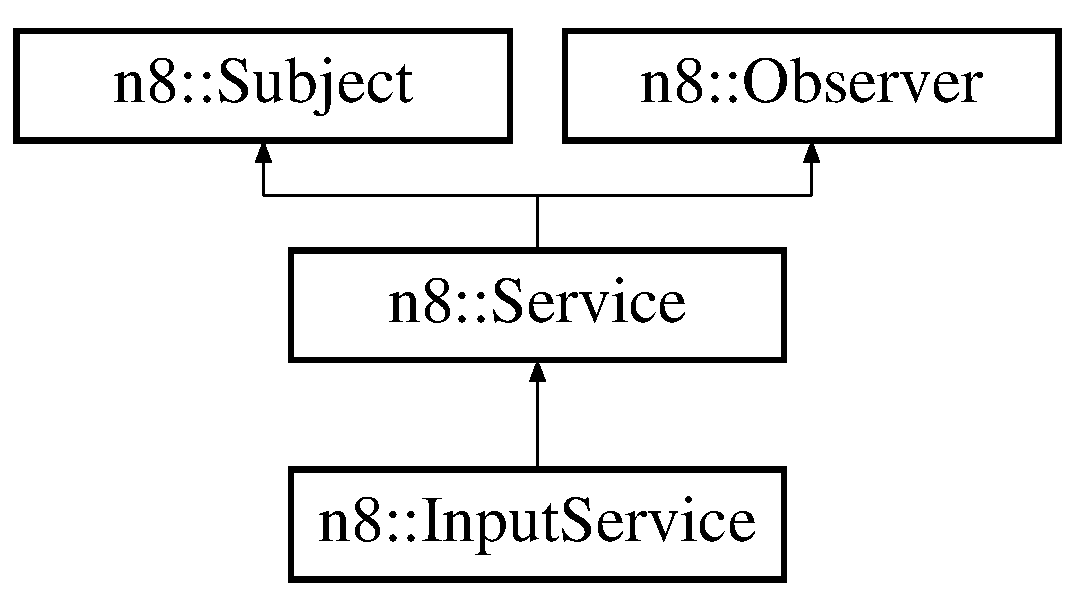
\includegraphics[height=3.000000cm]{classn8_1_1_input_service}
\end{center}
\end{figure}
\subsection*{Public Member Functions}
\begin{DoxyCompactItemize}
\item 
\hyperlink{classn8_1_1_input_service_a5f141dc8a07dde9ea917fd9c0ae48631}{Input\-Service} ()
\item 
\hyperlink{classn8_1_1_input_service_a11df32939e83610aec40636e4da4fe0c}{$\sim$\-Input\-Service} ()
\item 
void \hyperlink{classn8_1_1_input_service_ab8a0f93cf27cd8255bbb81993c5b3add}{Handle\-Input} ()
\item 
bool \hyperlink{classn8_1_1_input_service_a7c44294b125316e30398cdae2fb8bbb3}{Handle\-Event} ()
\item 
bool \hyperlink{classn8_1_1_input_service_a3b542975c80b74fc1088086645cf5415}{Key\-Is\-Down} (int key)
\item 
bool \hyperlink{classn8_1_1_input_service_a3ce5da16a67e2595a91167b533b7e074}{Key\-Is\-Up} (int key)
\item 
void \hyperlink{classn8_1_1_input_service_a8a5cc25bb823653ce6d4abb55a289cd3}{Register\-Key\-Up\-Command} (int, \hyperlink{classn8_1_1_command}{Command} $\ast$)
\item 
void \hyperlink{classn8_1_1_input_service_a1b0a32e9ed8f21c3138d69d07a9cf90c}{Register\-Key\-Down\-Command} (int, \hyperlink{classn8_1_1_command}{Command} $\ast$)
\item 
void \hyperlink{classn8_1_1_input_service_ab4a13fe0d3e6d6ed6642e7c9df77e884}{Unregister\-Key\-Commands} ()
\item 
void \hyperlink{classn8_1_1_input_service_aa52767bfd35d3785ea236c8175598212}{On\-Notify} (\hyperlink{classn8_1_1_event}{Event} $\ast$event)
\end{DoxyCompactItemize}
\subsection*{Private Member Functions}
\begin{DoxyCompactItemize}
\item 
bool \hyperlink{classn8_1_1_input_service_a3f04f6225455752a020818c9267442cc}{Key\-Is\-Down} (S\-D\-L\-\_\-\-Event $\ast$event, int key)
\item 
bool \hyperlink{classn8_1_1_input_service_a8f872d72b45d21e42cd6e7ef1b7c202a}{Key\-Is\-Up} (S\-D\-L\-\_\-\-Event $\ast$event, int key)
\end{DoxyCompactItemize}
\subsection*{Private Attributes}
\begin{DoxyCompactItemize}
\item 
S\-D\-L\-\_\-\-Event $\ast$ \hyperlink{classn8_1_1_input_service_a9eab1e8bff2306d4e581175d0d683184}{m\-\_\-event}
\item 
bool \hyperlink{classn8_1_1_input_service_ac35485b7fde20abe519f9deebc813eb2}{m\-\_\-keys\-Held} \mbox{[}323\mbox{]}
\item 
\hyperlink{classn8_1_1_command}{Command} $\ast$ \hyperlink{classn8_1_1_input_service_a7ac30fbb458b6b41138a1a9ae76e3497}{m\-\_\-registered\-Key\-Down\-Commands} \mbox{[}323\mbox{]}
\item 
\hyperlink{classn8_1_1_command}{Command} $\ast$ \hyperlink{classn8_1_1_input_service_a3f222cabde1339a524d0a9ca70bc1d3f}{m\-\_\-registered\-Key\-Up\-Commands} \mbox{[}323\mbox{]}
\end{DoxyCompactItemize}


\subsection{Constructor \& Destructor Documentation}
\hypertarget{classn8_1_1_input_service_a5f141dc8a07dde9ea917fd9c0ae48631}{\index{n8\-::\-Input\-Service@{n8\-::\-Input\-Service}!Input\-Service@{Input\-Service}}
\index{Input\-Service@{Input\-Service}!n8::InputService@{n8\-::\-Input\-Service}}
\subsubsection[{Input\-Service}]{\setlength{\rightskip}{0pt plus 5cm}n8\-::\-Input\-Service\-::\-Input\-Service (
\begin{DoxyParamCaption}
{}
\end{DoxyParamCaption}
)}}\label{classn8_1_1_input_service_a5f141dc8a07dde9ea917fd9c0ae48631}
Default constructor Initializes event\-\_\- \hypertarget{classn8_1_1_input_service_a11df32939e83610aec40636e4da4fe0c}{\index{n8\-::\-Input\-Service@{n8\-::\-Input\-Service}!$\sim$\-Input\-Service@{$\sim$\-Input\-Service}}
\index{$\sim$\-Input\-Service@{$\sim$\-Input\-Service}!n8::InputService@{n8\-::\-Input\-Service}}
\subsubsection[{$\sim$\-Input\-Service}]{\setlength{\rightskip}{0pt plus 5cm}n8\-::\-Input\-Service\-::$\sim$\-Input\-Service (
\begin{DoxyParamCaption}
{}
\end{DoxyParamCaption}
)}}\label{classn8_1_1_input_service_a11df32939e83610aec40636e4da4fe0c}
Default destructor 

\subsection{Member Function Documentation}
\hypertarget{classn8_1_1_input_service_a7c44294b125316e30398cdae2fb8bbb3}{\index{n8\-::\-Input\-Service@{n8\-::\-Input\-Service}!Handle\-Event@{Handle\-Event}}
\index{Handle\-Event@{Handle\-Event}!n8::InputService@{n8\-::\-Input\-Service}}
\subsubsection[{Handle\-Event}]{\setlength{\rightskip}{0pt plus 5cm}bool n8\-::\-Input\-Service\-::\-Handle\-Event (
\begin{DoxyParamCaption}
{}
\end{DoxyParamCaption}
)}}\label{classn8_1_1_input_service_a7c44294b125316e30398cdae2fb8bbb3}
\begin{DoxyReturn}{Returns}
True if there is an event in the queue 
\end{DoxyReturn}
\hypertarget{classn8_1_1_input_service_ab8a0f93cf27cd8255bbb81993c5b3add}{\index{n8\-::\-Input\-Service@{n8\-::\-Input\-Service}!Handle\-Input@{Handle\-Input}}
\index{Handle\-Input@{Handle\-Input}!n8::InputService@{n8\-::\-Input\-Service}}
\subsubsection[{Handle\-Input}]{\setlength{\rightskip}{0pt plus 5cm}void n8\-::\-Input\-Service\-::\-Handle\-Input (
\begin{DoxyParamCaption}
{}
\end{DoxyParamCaption}
)}}\label{classn8_1_1_input_service_ab8a0f93cf27cd8255bbb81993c5b3add}
Takes a polled event and tracks which events have occured so they can be responded to by a game state \hypertarget{classn8_1_1_input_service_a3b542975c80b74fc1088086645cf5415}{\index{n8\-::\-Input\-Service@{n8\-::\-Input\-Service}!Key\-Is\-Down@{Key\-Is\-Down}}
\index{Key\-Is\-Down@{Key\-Is\-Down}!n8::InputService@{n8\-::\-Input\-Service}}
\subsubsection[{Key\-Is\-Down}]{\setlength{\rightskip}{0pt plus 5cm}bool n8\-::\-Input\-Service\-::\-Key\-Is\-Down (
\begin{DoxyParamCaption}
\item[{int}]{key}
\end{DoxyParamCaption}
)}}\label{classn8_1_1_input_service_a3b542975c80b74fc1088086645cf5415}
Checks whether a key is pressed down Called by the user.


\begin{DoxyParams}{Parameters}
{\em key} & The key that is being checked\\
\hline
\end{DoxyParams}
\begin{DoxyReturn}{Returns}
True if the key was pressed down, False otherwise 
\end{DoxyReturn}
\hypertarget{classn8_1_1_input_service_a3f04f6225455752a020818c9267442cc}{\index{n8\-::\-Input\-Service@{n8\-::\-Input\-Service}!Key\-Is\-Down@{Key\-Is\-Down}}
\index{Key\-Is\-Down@{Key\-Is\-Down}!n8::InputService@{n8\-::\-Input\-Service}}
\subsubsection[{Key\-Is\-Down}]{\setlength{\rightskip}{0pt plus 5cm}bool n8\-::\-Input\-Service\-::\-Key\-Is\-Down (
\begin{DoxyParamCaption}
\item[{S\-D\-L\-\_\-\-Event $\ast$}]{event, }
\item[{int}]{key}
\end{DoxyParamCaption}
)\hspace{0.3cm}{\ttfamily [private]}}}\label{classn8_1_1_input_service_a3f04f6225455752a020818c9267442cc}
Checks whether a key is pressed down Called internally by \hyperlink{classn8_1_1_input_service_a3b542975c80b74fc1088086645cf5415}{Key\-Is\-Down(int key)}.


\begin{DoxyParams}{Parameters}
{\em event} & The event object storing event information \\
\hline
{\em key} & The key that is being checked\\
\hline
\end{DoxyParams}
\begin{DoxyReturn}{Returns}
True if the specified key was pressed down, False otherwise 
\end{DoxyReturn}
\hypertarget{classn8_1_1_input_service_a3ce5da16a67e2595a91167b533b7e074}{\index{n8\-::\-Input\-Service@{n8\-::\-Input\-Service}!Key\-Is\-Up@{Key\-Is\-Up}}
\index{Key\-Is\-Up@{Key\-Is\-Up}!n8::InputService@{n8\-::\-Input\-Service}}
\subsubsection[{Key\-Is\-Up}]{\setlength{\rightskip}{0pt plus 5cm}bool n8\-::\-Input\-Service\-::\-Key\-Is\-Up (
\begin{DoxyParamCaption}
\item[{int}]{key}
\end{DoxyParamCaption}
)}}\label{classn8_1_1_input_service_a3ce5da16a67e2595a91167b533b7e074}
Checks whether a key is up Called by the user.


\begin{DoxyParams}{Parameters}
{\em key} & The key that is being checked\\
\hline
\end{DoxyParams}
\begin{DoxyReturn}{Returns}
True if the key is up, False otherwise 
\end{DoxyReturn}
\hypertarget{classn8_1_1_input_service_a8f872d72b45d21e42cd6e7ef1b7c202a}{\index{n8\-::\-Input\-Service@{n8\-::\-Input\-Service}!Key\-Is\-Up@{Key\-Is\-Up}}
\index{Key\-Is\-Up@{Key\-Is\-Up}!n8::InputService@{n8\-::\-Input\-Service}}
\subsubsection[{Key\-Is\-Up}]{\setlength{\rightskip}{0pt plus 5cm}bool n8\-::\-Input\-Service\-::\-Key\-Is\-Up (
\begin{DoxyParamCaption}
\item[{S\-D\-L\-\_\-\-Event $\ast$}]{event, }
\item[{int}]{key}
\end{DoxyParamCaption}
)\hspace{0.3cm}{\ttfamily [private]}}}\label{classn8_1_1_input_service_a8f872d72b45d21e42cd6e7ef1b7c202a}
Checks whether a key is up Called internally by \hyperlink{classn8_1_1_input_service_a3ce5da16a67e2595a91167b533b7e074}{Key\-Is\-Up(int key)}.


\begin{DoxyParams}{Parameters}
{\em event} & The event object storing event information \\
\hline
{\em key} & The key that is being checked\\
\hline
\end{DoxyParams}
\begin{DoxyReturn}{Returns}
True if the specified key is up, False otherwise 
\end{DoxyReturn}
\hypertarget{classn8_1_1_input_service_aa52767bfd35d3785ea236c8175598212}{\index{n8\-::\-Input\-Service@{n8\-::\-Input\-Service}!On\-Notify@{On\-Notify}}
\index{On\-Notify@{On\-Notify}!n8::InputService@{n8\-::\-Input\-Service}}
\subsubsection[{On\-Notify}]{\setlength{\rightskip}{0pt plus 5cm}void n8\-::\-Input\-Service\-::\-On\-Notify (
\begin{DoxyParamCaption}
\item[{{\bf Event} $\ast$}]{event}
\end{DoxyParamCaption}
)\hspace{0.3cm}{\ttfamily [virtual]}}}\label{classn8_1_1_input_service_aa52767bfd35d3785ea236c8175598212}


Implements \hyperlink{classn8_1_1_service_a756a170eba7e5c34a1c12008e22d3ca7}{n8\-::\-Service}.

\hypertarget{classn8_1_1_input_service_a1b0a32e9ed8f21c3138d69d07a9cf90c}{\index{n8\-::\-Input\-Service@{n8\-::\-Input\-Service}!Register\-Key\-Down\-Command@{Register\-Key\-Down\-Command}}
\index{Register\-Key\-Down\-Command@{Register\-Key\-Down\-Command}!n8::InputService@{n8\-::\-Input\-Service}}
\subsubsection[{Register\-Key\-Down\-Command}]{\setlength{\rightskip}{0pt plus 5cm}void n8\-::\-Input\-Service\-::\-Register\-Key\-Down\-Command (
\begin{DoxyParamCaption}
\item[{int}]{key, }
\item[{{\bf Command} $\ast$}]{command}
\end{DoxyParamCaption}
)}}\label{classn8_1_1_input_service_a1b0a32e9ed8f21c3138d69d07a9cf90c}
\hypertarget{classn8_1_1_input_service_a8a5cc25bb823653ce6d4abb55a289cd3}{\index{n8\-::\-Input\-Service@{n8\-::\-Input\-Service}!Register\-Key\-Up\-Command@{Register\-Key\-Up\-Command}}
\index{Register\-Key\-Up\-Command@{Register\-Key\-Up\-Command}!n8::InputService@{n8\-::\-Input\-Service}}
\subsubsection[{Register\-Key\-Up\-Command}]{\setlength{\rightskip}{0pt plus 5cm}void n8\-::\-Input\-Service\-::\-Register\-Key\-Up\-Command (
\begin{DoxyParamCaption}
\item[{int}]{key, }
\item[{{\bf Command} $\ast$}]{command}
\end{DoxyParamCaption}
)}}\label{classn8_1_1_input_service_a8a5cc25bb823653ce6d4abb55a289cd3}
\hypertarget{classn8_1_1_input_service_ab4a13fe0d3e6d6ed6642e7c9df77e884}{\index{n8\-::\-Input\-Service@{n8\-::\-Input\-Service}!Unregister\-Key\-Commands@{Unregister\-Key\-Commands}}
\index{Unregister\-Key\-Commands@{Unregister\-Key\-Commands}!n8::InputService@{n8\-::\-Input\-Service}}
\subsubsection[{Unregister\-Key\-Commands}]{\setlength{\rightskip}{0pt plus 5cm}void n8\-::\-Input\-Service\-::\-Unregister\-Key\-Commands (
\begin{DoxyParamCaption}
{}
\end{DoxyParamCaption}
)}}\label{classn8_1_1_input_service_ab4a13fe0d3e6d6ed6642e7c9df77e884}


\subsection{Member Data Documentation}
\hypertarget{classn8_1_1_input_service_a9eab1e8bff2306d4e581175d0d683184}{\index{n8\-::\-Input\-Service@{n8\-::\-Input\-Service}!m\-\_\-event@{m\-\_\-event}}
\index{m\-\_\-event@{m\-\_\-event}!n8::InputService@{n8\-::\-Input\-Service}}
\subsubsection[{m\-\_\-event}]{\setlength{\rightskip}{0pt plus 5cm}S\-D\-L\-\_\-\-Event$\ast$ n8\-::\-Input\-Service\-::m\-\_\-event\hspace{0.3cm}{\ttfamily [private]}}}\label{classn8_1_1_input_service_a9eab1e8bff2306d4e581175d0d683184}
\hypertarget{classn8_1_1_input_service_ac35485b7fde20abe519f9deebc813eb2}{\index{n8\-::\-Input\-Service@{n8\-::\-Input\-Service}!m\-\_\-keys\-Held@{m\-\_\-keys\-Held}}
\index{m\-\_\-keys\-Held@{m\-\_\-keys\-Held}!n8::InputService@{n8\-::\-Input\-Service}}
\subsubsection[{m\-\_\-keys\-Held}]{\setlength{\rightskip}{0pt plus 5cm}bool n8\-::\-Input\-Service\-::m\-\_\-keys\-Held\mbox{[}323\mbox{]}\hspace{0.3cm}{\ttfamily [private]}}}\label{classn8_1_1_input_service_ac35485b7fde20abe519f9deebc813eb2}
$<$ S\-D\-L\-\_\-\-Event pointer to get dequeued events \hypertarget{classn8_1_1_input_service_a7ac30fbb458b6b41138a1a9ae76e3497}{\index{n8\-::\-Input\-Service@{n8\-::\-Input\-Service}!m\-\_\-registered\-Key\-Down\-Commands@{m\-\_\-registered\-Key\-Down\-Commands}}
\index{m\-\_\-registered\-Key\-Down\-Commands@{m\-\_\-registered\-Key\-Down\-Commands}!n8::InputService@{n8\-::\-Input\-Service}}
\subsubsection[{m\-\_\-registered\-Key\-Down\-Commands}]{\setlength{\rightskip}{0pt plus 5cm}{\bf Command}$\ast$ n8\-::\-Input\-Service\-::m\-\_\-registered\-Key\-Down\-Commands\mbox{[}323\mbox{]}\hspace{0.3cm}{\ttfamily [private]}}}\label{classn8_1_1_input_service_a7ac30fbb458b6b41138a1a9ae76e3497}
$<$ Array to store whether or not a key is being held down \hypertarget{classn8_1_1_input_service_a3f222cabde1339a524d0a9ca70bc1d3f}{\index{n8\-::\-Input\-Service@{n8\-::\-Input\-Service}!m\-\_\-registered\-Key\-Up\-Commands@{m\-\_\-registered\-Key\-Up\-Commands}}
\index{m\-\_\-registered\-Key\-Up\-Commands@{m\-\_\-registered\-Key\-Up\-Commands}!n8::InputService@{n8\-::\-Input\-Service}}
\subsubsection[{m\-\_\-registered\-Key\-Up\-Commands}]{\setlength{\rightskip}{0pt plus 5cm}{\bf Command}$\ast$ n8\-::\-Input\-Service\-::m\-\_\-registered\-Key\-Up\-Commands\mbox{[}323\mbox{]}\hspace{0.3cm}{\ttfamily [private]}}}\label{classn8_1_1_input_service_a3f222cabde1339a524d0a9ca70bc1d3f}


The documentation for this class was generated from the following files\-:\begin{DoxyCompactItemize}
\item 
Services/\hyperlink{_input_service_8h}{Input\-Service.\-h}\item 
Services/\hyperlink{_input_service_8cpp}{Input\-Service.\-cpp}\end{DoxyCompactItemize}

\hypertarget{classn8_1_1_log}{\section{n8\-:\-:Log Class Reference}
\label{classn8_1_1_log}\index{n8\-::\-Log@{n8\-::\-Log}}
}


{\ttfamily \#include $<$Log.\-h$>$}

Inheritance diagram for n8\-:\-:Log\-:\begin{figure}[H]
\begin{center}
\leavevmode
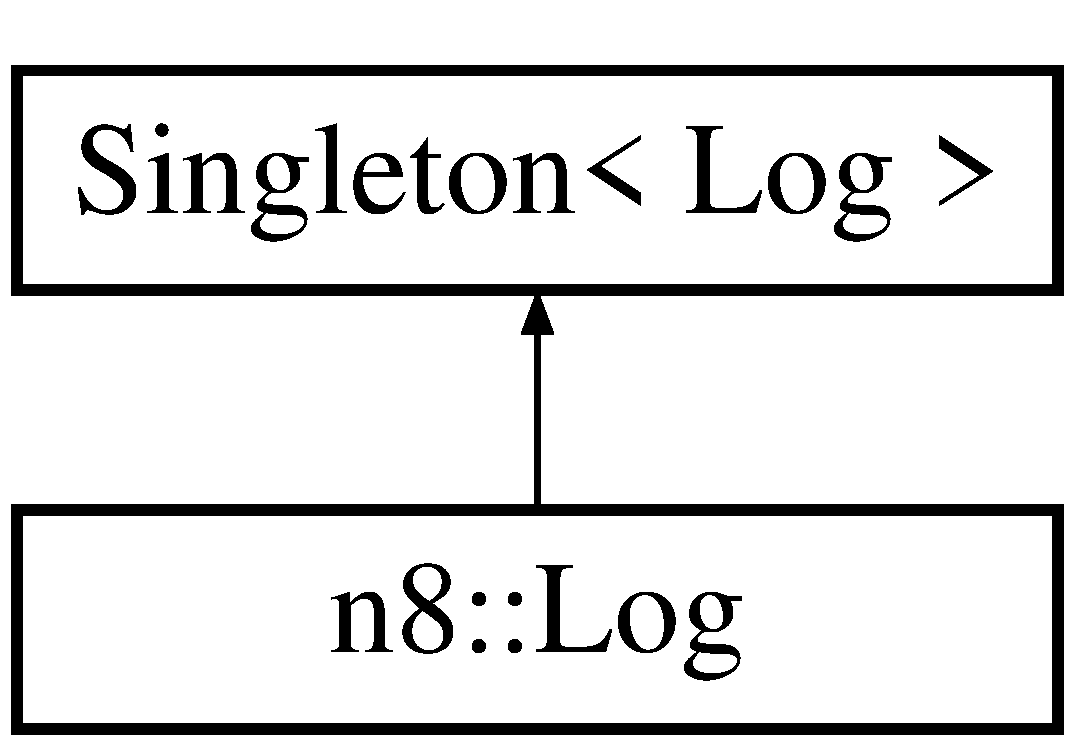
\includegraphics[height=2.000000cm]{classn8_1_1_log}
\end{center}
\end{figure}
\subsection*{Public Member Functions}
\begin{DoxyCompactItemize}
\item 
\hyperlink{classn8_1_1_log_adf2aa71acae5a706ec4e62506e851bb5}{Log} ()
\item 
virtual \hyperlink{classn8_1_1_log_aa29b98fa3440f61ef636a79c23193cb3}{$\sim$\-Log} ()
\end{DoxyCompactItemize}
\subsection*{Static Public Member Functions}
\begin{DoxyCompactItemize}
\item 
static void \hyperlink{classn8_1_1_log_aaa8658e983713fcf8a4aab1fb76c31e3}{Error} (std\-::string tag, std\-::string msg)
\item 
static void \hyperlink{classn8_1_1_log_a97be57e8b2c04da6f47f1e699c827024}{Info} (std\-::string tag, std\-::string msg)
\item 
static void \hyperlink{classn8_1_1_log_ac7e56dd29823f4f0fc2b3a884f575737}{Debug} (std\-::string tag, std\-::string msg)
\item 
static void \hyperlink{classn8_1_1_log_a816be7956f40290b2f4e1b9eeb60b93b}{Turn\-On\-Error\-Messages} ()
\item 
static void \hyperlink{classn8_1_1_log_ad75994d1eca6ff1f1efb4358f62ae88c}{Turn\-Off\-Error\-Messages} ()
\item 
static void \hyperlink{classn8_1_1_log_a47119603ba767c51e547cfbae28d0c97}{Turn\-On\-Info\-Messages} ()
\item 
static void \hyperlink{classn8_1_1_log_a1c455a4fa66ea6148897dabe97cf6352}{Turn\-Off\-Info\-Messages} ()
\item 
static void \hyperlink{classn8_1_1_log_a4e636f7659828b0c16add87aeec9bb6a}{Turn\-On\-Debugging\-Messages} ()
\item 
static void \hyperlink{classn8_1_1_log_ae47bf8c5ff5f6e94433c4741be939dab}{Turn\-Off\-Debugging\-Messages} ()
\end{DoxyCompactItemize}
\subsection*{Static Private Attributes}
\begin{DoxyCompactItemize}
\item 
static bool \hyperlink{classn8_1_1_log_a55e19b41d018681126fbdf7e67133120}{E\-R\-R\-O\-R} = true
\item 
static bool \hyperlink{classn8_1_1_log_a5784cbe90ebfbfc2c0293be4aefc37df}{I\-N\-F\-O} = true
\item 
static bool \hyperlink{classn8_1_1_log_a8169e40180cf2f69e873b7e91c71df3d}{D\-E\-B\-U\-G\-G\-I\-N\-G} = true
\end{DoxyCompactItemize}
\subsection*{Additional Inherited Members}


\subsection{Detailed Description}
Provides static logging functionality. Could be extended to allow for runtime logging. 

\subsection{Constructor \& Destructor Documentation}
\hypertarget{classn8_1_1_log_adf2aa71acae5a706ec4e62506e851bb5}{\index{n8\-::\-Log@{n8\-::\-Log}!Log@{Log}}
\index{Log@{Log}!n8::Log@{n8\-::\-Log}}
\subsubsection[{Log}]{\setlength{\rightskip}{0pt plus 5cm}n8\-::\-Log\-::\-Log (
\begin{DoxyParamCaption}
{}
\end{DoxyParamCaption}
)}}\label{classn8_1_1_log_adf2aa71acae5a706ec4e62506e851bb5}
\hypertarget{classn8_1_1_log_aa29b98fa3440f61ef636a79c23193cb3}{\index{n8\-::\-Log@{n8\-::\-Log}!$\sim$\-Log@{$\sim$\-Log}}
\index{$\sim$\-Log@{$\sim$\-Log}!n8::Log@{n8\-::\-Log}}
\subsubsection[{$\sim$\-Log}]{\setlength{\rightskip}{0pt plus 5cm}n8\-::\-Log\-::$\sim$\-Log (
\begin{DoxyParamCaption}
{}
\end{DoxyParamCaption}
)\hspace{0.3cm}{\ttfamily [virtual]}}}\label{classn8_1_1_log_aa29b98fa3440f61ef636a79c23193cb3}


\subsection{Member Function Documentation}
\hypertarget{classn8_1_1_log_ac7e56dd29823f4f0fc2b3a884f575737}{\index{n8\-::\-Log@{n8\-::\-Log}!Debug@{Debug}}
\index{Debug@{Debug}!n8::Log@{n8\-::\-Log}}
\subsubsection[{Debug}]{\setlength{\rightskip}{0pt plus 5cm}void n8\-::\-Log\-::\-Debug (
\begin{DoxyParamCaption}
\item[{std\-::string}]{tag, }
\item[{std\-::string}]{msg}
\end{DoxyParamCaption}
)\hspace{0.3cm}{\ttfamily [static]}}}\label{classn8_1_1_log_ac7e56dd29823f4f0fc2b3a884f575737}
Used to print debug messages to the console


\begin{DoxyParams}{Parameters}
{\em tag} & A string to indicate something about the message such as the class, method, or file it's from \\
\hline
{\em msg} & The message to print \\
\hline
\end{DoxyParams}
\hypertarget{classn8_1_1_log_aaa8658e983713fcf8a4aab1fb76c31e3}{\index{n8\-::\-Log@{n8\-::\-Log}!Error@{Error}}
\index{Error@{Error}!n8::Log@{n8\-::\-Log}}
\subsubsection[{Error}]{\setlength{\rightskip}{0pt plus 5cm}void n8\-::\-Log\-::\-Error (
\begin{DoxyParamCaption}
\item[{std\-::string}]{tag, }
\item[{std\-::string}]{msg}
\end{DoxyParamCaption}
)\hspace{0.3cm}{\ttfamily [static]}}}\label{classn8_1_1_log_aaa8658e983713fcf8a4aab1fb76c31e3}
Used to print error messages to the console


\begin{DoxyParams}{Parameters}
{\em tag} & A string to indicate something about the message such as the class, method, or file it's from \\
\hline
{\em msg} & The message to print describing the error \\
\hline
\end{DoxyParams}
\hypertarget{classn8_1_1_log_a97be57e8b2c04da6f47f1e699c827024}{\index{n8\-::\-Log@{n8\-::\-Log}!Info@{Info}}
\index{Info@{Info}!n8::Log@{n8\-::\-Log}}
\subsubsection[{Info}]{\setlength{\rightskip}{0pt plus 5cm}void n8\-::\-Log\-::\-Info (
\begin{DoxyParamCaption}
\item[{std\-::string}]{tag, }
\item[{std\-::string}]{msg}
\end{DoxyParamCaption}
)\hspace{0.3cm}{\ttfamily [static]}}}\label{classn8_1_1_log_a97be57e8b2c04da6f47f1e699c827024}
Used to print info messages to the console


\begin{DoxyParams}{Parameters}
{\em tag} & A string to indicate something about the message such as the class, method, or file it's from \\
\hline
{\em msg} & The message to print \\
\hline
\end{DoxyParams}
\hypertarget{classn8_1_1_log_ae47bf8c5ff5f6e94433c4741be939dab}{\index{n8\-::\-Log@{n8\-::\-Log}!Turn\-Off\-Debugging\-Messages@{Turn\-Off\-Debugging\-Messages}}
\index{Turn\-Off\-Debugging\-Messages@{Turn\-Off\-Debugging\-Messages}!n8::Log@{n8\-::\-Log}}
\subsubsection[{Turn\-Off\-Debugging\-Messages}]{\setlength{\rightskip}{0pt plus 5cm}void n8\-::\-Log\-::\-Turn\-Off\-Debugging\-Messages (
\begin{DoxyParamCaption}
{}
\end{DoxyParamCaption}
)\hspace{0.3cm}{\ttfamily [static]}}}\label{classn8_1_1_log_ae47bf8c5ff5f6e94433c4741be939dab}
Sets the D\-E\-B\-U\-G\-G\-I\-N\-G flag to false This causes debugging messages to not be displayed \hypertarget{classn8_1_1_log_ad75994d1eca6ff1f1efb4358f62ae88c}{\index{n8\-::\-Log@{n8\-::\-Log}!Turn\-Off\-Error\-Messages@{Turn\-Off\-Error\-Messages}}
\index{Turn\-Off\-Error\-Messages@{Turn\-Off\-Error\-Messages}!n8::Log@{n8\-::\-Log}}
\subsubsection[{Turn\-Off\-Error\-Messages}]{\setlength{\rightskip}{0pt plus 5cm}void n8\-::\-Log\-::\-Turn\-Off\-Error\-Messages (
\begin{DoxyParamCaption}
{}
\end{DoxyParamCaption}
)\hspace{0.3cm}{\ttfamily [static]}}}\label{classn8_1_1_log_ad75994d1eca6ff1f1efb4358f62ae88c}
Sets the E\-R\-R\-O\-R flag to false This causes error messages to not be displayed \hypertarget{classn8_1_1_log_a1c455a4fa66ea6148897dabe97cf6352}{\index{n8\-::\-Log@{n8\-::\-Log}!Turn\-Off\-Info\-Messages@{Turn\-Off\-Info\-Messages}}
\index{Turn\-Off\-Info\-Messages@{Turn\-Off\-Info\-Messages}!n8::Log@{n8\-::\-Log}}
\subsubsection[{Turn\-Off\-Info\-Messages}]{\setlength{\rightskip}{0pt plus 5cm}void n8\-::\-Log\-::\-Turn\-Off\-Info\-Messages (
\begin{DoxyParamCaption}
{}
\end{DoxyParamCaption}
)\hspace{0.3cm}{\ttfamily [static]}}}\label{classn8_1_1_log_a1c455a4fa66ea6148897dabe97cf6352}
Sets the I\-N\-F\-O flag to false This causes info messages to not be displayed \hypertarget{classn8_1_1_log_a4e636f7659828b0c16add87aeec9bb6a}{\index{n8\-::\-Log@{n8\-::\-Log}!Turn\-On\-Debugging\-Messages@{Turn\-On\-Debugging\-Messages}}
\index{Turn\-On\-Debugging\-Messages@{Turn\-On\-Debugging\-Messages}!n8::Log@{n8\-::\-Log}}
\subsubsection[{Turn\-On\-Debugging\-Messages}]{\setlength{\rightskip}{0pt plus 5cm}void n8\-::\-Log\-::\-Turn\-On\-Debugging\-Messages (
\begin{DoxyParamCaption}
{}
\end{DoxyParamCaption}
)\hspace{0.3cm}{\ttfamily [static]}}}\label{classn8_1_1_log_a4e636f7659828b0c16add87aeec9bb6a}
Sets the D\-E\-B\-U\-G\-G\-I\-N\-G flag to true. This allows debugging messages to be displayed \hypertarget{classn8_1_1_log_a816be7956f40290b2f4e1b9eeb60b93b}{\index{n8\-::\-Log@{n8\-::\-Log}!Turn\-On\-Error\-Messages@{Turn\-On\-Error\-Messages}}
\index{Turn\-On\-Error\-Messages@{Turn\-On\-Error\-Messages}!n8::Log@{n8\-::\-Log}}
\subsubsection[{Turn\-On\-Error\-Messages}]{\setlength{\rightskip}{0pt plus 5cm}void n8\-::\-Log\-::\-Turn\-On\-Error\-Messages (
\begin{DoxyParamCaption}
{}
\end{DoxyParamCaption}
)\hspace{0.3cm}{\ttfamily [static]}}}\label{classn8_1_1_log_a816be7956f40290b2f4e1b9eeb60b93b}
Sets the E\-R\-R\-O\-R flag to true. This allows error messages to be displayed \hypertarget{classn8_1_1_log_a47119603ba767c51e547cfbae28d0c97}{\index{n8\-::\-Log@{n8\-::\-Log}!Turn\-On\-Info\-Messages@{Turn\-On\-Info\-Messages}}
\index{Turn\-On\-Info\-Messages@{Turn\-On\-Info\-Messages}!n8::Log@{n8\-::\-Log}}
\subsubsection[{Turn\-On\-Info\-Messages}]{\setlength{\rightskip}{0pt plus 5cm}void n8\-::\-Log\-::\-Turn\-On\-Info\-Messages (
\begin{DoxyParamCaption}
{}
\end{DoxyParamCaption}
)\hspace{0.3cm}{\ttfamily [static]}}}\label{classn8_1_1_log_a47119603ba767c51e547cfbae28d0c97}
Sets the I\-N\-F\-O flag to true. This allows info messages to be displayed 

\subsection{Member Data Documentation}
\hypertarget{classn8_1_1_log_a8169e40180cf2f69e873b7e91c71df3d}{\index{n8\-::\-Log@{n8\-::\-Log}!D\-E\-B\-U\-G\-G\-I\-N\-G@{D\-E\-B\-U\-G\-G\-I\-N\-G}}
\index{D\-E\-B\-U\-G\-G\-I\-N\-G@{D\-E\-B\-U\-G\-G\-I\-N\-G}!n8::Log@{n8\-::\-Log}}
\subsubsection[{D\-E\-B\-U\-G\-G\-I\-N\-G}]{\setlength{\rightskip}{0pt plus 5cm}bool n8\-::\-Log\-::\-D\-E\-B\-U\-G\-G\-I\-N\-G = true\hspace{0.3cm}{\ttfamily [static]}, {\ttfamily [private]}}}\label{classn8_1_1_log_a8169e40180cf2f69e873b7e91c71df3d}
$<$ static boolean flag to control whether I\-N\-F\-O messages are displayed $>$ \hypertarget{classn8_1_1_log_a55e19b41d018681126fbdf7e67133120}{\index{n8\-::\-Log@{n8\-::\-Log}!E\-R\-R\-O\-R@{E\-R\-R\-O\-R}}
\index{E\-R\-R\-O\-R@{E\-R\-R\-O\-R}!n8::Log@{n8\-::\-Log}}
\subsubsection[{E\-R\-R\-O\-R}]{\setlength{\rightskip}{0pt plus 5cm}bool n8\-::\-Log\-::\-E\-R\-R\-O\-R = true\hspace{0.3cm}{\ttfamily [static]}, {\ttfamily [private]}}}\label{classn8_1_1_log_a55e19b41d018681126fbdf7e67133120}
\hypertarget{classn8_1_1_log_a5784cbe90ebfbfc2c0293be4aefc37df}{\index{n8\-::\-Log@{n8\-::\-Log}!I\-N\-F\-O@{I\-N\-F\-O}}
\index{I\-N\-F\-O@{I\-N\-F\-O}!n8::Log@{n8\-::\-Log}}
\subsubsection[{I\-N\-F\-O}]{\setlength{\rightskip}{0pt plus 5cm}bool n8\-::\-Log\-::\-I\-N\-F\-O = true\hspace{0.3cm}{\ttfamily [static]}, {\ttfamily [private]}}}\label{classn8_1_1_log_a5784cbe90ebfbfc2c0293be4aefc37df}
$<$ static boolean flag to control whether E\-R\-R\-O\-R messages are displayed $>$ 

The documentation for this class was generated from the following files\-:\begin{DoxyCompactItemize}
\item 
Utils/\hyperlink{_log_8h}{Log.\-h}\item 
Utils/\hyperlink{_log_8cpp}{Log.\-cpp}\end{DoxyCompactItemize}

\hypertarget{classtinyxml2_1_1_mem_pool}{\section{tinyxml2\-:\-:Mem\-Pool Class Reference}
\label{classtinyxml2_1_1_mem_pool}\index{tinyxml2\-::\-Mem\-Pool@{tinyxml2\-::\-Mem\-Pool}}
}


{\ttfamily \#include $<$tinyxml2.\-h$>$}

Inheritance diagram for tinyxml2\-:\-:Mem\-Pool\-:\begin{figure}[H]
\begin{center}
\leavevmode
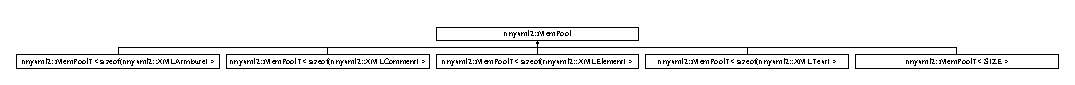
\includegraphics[height=0.691358cm]{classtinyxml2_1_1_mem_pool}
\end{center}
\end{figure}
\subsection*{Public Member Functions}
\begin{DoxyCompactItemize}
\item 
\hyperlink{classtinyxml2_1_1_mem_pool_a9101a0083d7370c85bd5aaaba7157f84}{Mem\-Pool} ()
\item 
virtual \hyperlink{classtinyxml2_1_1_mem_pool_ae55ad9e3faeca702e6ccbb38fdbcad72}{$\sim$\-Mem\-Pool} ()
\item 
virtual int \hyperlink{classtinyxml2_1_1_mem_pool_a0c518d49e3a94bde566f61e13b7240bb}{Item\-Size} () const =0
\item 
virtual void $\ast$ \hyperlink{classtinyxml2_1_1_mem_pool_a4f977b5fed752c0bbfe5295f469d6449}{Alloc} ()=0
\item 
virtual void \hyperlink{classtinyxml2_1_1_mem_pool_a49e3bfac2cba2ebd6776b31e571f64f7}{Free} (void $\ast$)=0
\item 
virtual void \hyperlink{classtinyxml2_1_1_mem_pool_ac5804dd1387b2e4de5eef710076a0db1}{Set\-Tracked} ()=0
\end{DoxyCompactItemize}


\subsection{Constructor \& Destructor Documentation}
\hypertarget{classtinyxml2_1_1_mem_pool_a9101a0083d7370c85bd5aaaba7157f84}{\index{tinyxml2\-::\-Mem\-Pool@{tinyxml2\-::\-Mem\-Pool}!Mem\-Pool@{Mem\-Pool}}
\index{Mem\-Pool@{Mem\-Pool}!tinyxml2::MemPool@{tinyxml2\-::\-Mem\-Pool}}
\subsubsection[{Mem\-Pool}]{\setlength{\rightskip}{0pt plus 5cm}tinyxml2\-::\-Mem\-Pool\-::\-Mem\-Pool (
\begin{DoxyParamCaption}
{}
\end{DoxyParamCaption}
)\hspace{0.3cm}{\ttfamily [inline]}}}\label{classtinyxml2_1_1_mem_pool_a9101a0083d7370c85bd5aaaba7157f84}
\hypertarget{classtinyxml2_1_1_mem_pool_ae55ad9e3faeca702e6ccbb38fdbcad72}{\index{tinyxml2\-::\-Mem\-Pool@{tinyxml2\-::\-Mem\-Pool}!$\sim$\-Mem\-Pool@{$\sim$\-Mem\-Pool}}
\index{$\sim$\-Mem\-Pool@{$\sim$\-Mem\-Pool}!tinyxml2::MemPool@{tinyxml2\-::\-Mem\-Pool}}
\subsubsection[{$\sim$\-Mem\-Pool}]{\setlength{\rightskip}{0pt plus 5cm}virtual tinyxml2\-::\-Mem\-Pool\-::$\sim$\-Mem\-Pool (
\begin{DoxyParamCaption}
{}
\end{DoxyParamCaption}
)\hspace{0.3cm}{\ttfamily [inline]}, {\ttfamily [virtual]}}}\label{classtinyxml2_1_1_mem_pool_ae55ad9e3faeca702e6ccbb38fdbcad72}


\subsection{Member Function Documentation}
\hypertarget{classtinyxml2_1_1_mem_pool_a4f977b5fed752c0bbfe5295f469d6449}{\index{tinyxml2\-::\-Mem\-Pool@{tinyxml2\-::\-Mem\-Pool}!Alloc@{Alloc}}
\index{Alloc@{Alloc}!tinyxml2::MemPool@{tinyxml2\-::\-Mem\-Pool}}
\subsubsection[{Alloc}]{\setlength{\rightskip}{0pt plus 5cm}virtual void$\ast$ tinyxml2\-::\-Mem\-Pool\-::\-Alloc (
\begin{DoxyParamCaption}
{}
\end{DoxyParamCaption}
)\hspace{0.3cm}{\ttfamily [pure virtual]}}}\label{classtinyxml2_1_1_mem_pool_a4f977b5fed752c0bbfe5295f469d6449}


Implemented in \hyperlink{classtinyxml2_1_1_mem_pool_t_aa9d785a48ffe6ea1be679bab13464486}{tinyxml2\-::\-Mem\-Pool\-T$<$ S\-I\-Z\-E $>$}, \hyperlink{classtinyxml2_1_1_mem_pool_t_aa9d785a48ffe6ea1be679bab13464486}{tinyxml2\-::\-Mem\-Pool\-T$<$ sizeof(tinyxml2\-::\-X\-M\-L\-Comment) $>$}, \hyperlink{classtinyxml2_1_1_mem_pool_t_aa9d785a48ffe6ea1be679bab13464486}{tinyxml2\-::\-Mem\-Pool\-T$<$ sizeof(tinyxml2\-::\-X\-M\-L\-Text) $>$}, \hyperlink{classtinyxml2_1_1_mem_pool_t_aa9d785a48ffe6ea1be679bab13464486}{tinyxml2\-::\-Mem\-Pool\-T$<$ sizeof(tinyxml2\-::\-X\-M\-L\-Attribute) $>$}, and \hyperlink{classtinyxml2_1_1_mem_pool_t_aa9d785a48ffe6ea1be679bab13464486}{tinyxml2\-::\-Mem\-Pool\-T$<$ sizeof(tinyxml2\-::\-X\-M\-L\-Element) $>$}.

\hypertarget{classtinyxml2_1_1_mem_pool_a49e3bfac2cba2ebd6776b31e571f64f7}{\index{tinyxml2\-::\-Mem\-Pool@{tinyxml2\-::\-Mem\-Pool}!Free@{Free}}
\index{Free@{Free}!tinyxml2::MemPool@{tinyxml2\-::\-Mem\-Pool}}
\subsubsection[{Free}]{\setlength{\rightskip}{0pt plus 5cm}virtual void tinyxml2\-::\-Mem\-Pool\-::\-Free (
\begin{DoxyParamCaption}
\item[{void $\ast$}]{}
\end{DoxyParamCaption}
)\hspace{0.3cm}{\ttfamily [pure virtual]}}}\label{classtinyxml2_1_1_mem_pool_a49e3bfac2cba2ebd6776b31e571f64f7}


Implemented in \hyperlink{classtinyxml2_1_1_mem_pool_t_a4f1a0c434e9e3d7391e5c16ed4ee8c70}{tinyxml2\-::\-Mem\-Pool\-T$<$ S\-I\-Z\-E $>$}, \hyperlink{classtinyxml2_1_1_mem_pool_t_a4f1a0c434e9e3d7391e5c16ed4ee8c70}{tinyxml2\-::\-Mem\-Pool\-T$<$ sizeof(tinyxml2\-::\-X\-M\-L\-Comment) $>$}, \hyperlink{classtinyxml2_1_1_mem_pool_t_a4f1a0c434e9e3d7391e5c16ed4ee8c70}{tinyxml2\-::\-Mem\-Pool\-T$<$ sizeof(tinyxml2\-::\-X\-M\-L\-Text) $>$}, \hyperlink{classtinyxml2_1_1_mem_pool_t_a4f1a0c434e9e3d7391e5c16ed4ee8c70}{tinyxml2\-::\-Mem\-Pool\-T$<$ sizeof(tinyxml2\-::\-X\-M\-L\-Attribute) $>$}, and \hyperlink{classtinyxml2_1_1_mem_pool_t_a4f1a0c434e9e3d7391e5c16ed4ee8c70}{tinyxml2\-::\-Mem\-Pool\-T$<$ sizeof(tinyxml2\-::\-X\-M\-L\-Element) $>$}.

\hypertarget{classtinyxml2_1_1_mem_pool_a0c518d49e3a94bde566f61e13b7240bb}{\index{tinyxml2\-::\-Mem\-Pool@{tinyxml2\-::\-Mem\-Pool}!Item\-Size@{Item\-Size}}
\index{Item\-Size@{Item\-Size}!tinyxml2::MemPool@{tinyxml2\-::\-Mem\-Pool}}
\subsubsection[{Item\-Size}]{\setlength{\rightskip}{0pt plus 5cm}virtual int tinyxml2\-::\-Mem\-Pool\-::\-Item\-Size (
\begin{DoxyParamCaption}
{}
\end{DoxyParamCaption}
) const\hspace{0.3cm}{\ttfamily [pure virtual]}}}\label{classtinyxml2_1_1_mem_pool_a0c518d49e3a94bde566f61e13b7240bb}


Implemented in \hyperlink{classtinyxml2_1_1_mem_pool_t_a7ec8778fe99f6e332615a703be0b48bc}{tinyxml2\-::\-Mem\-Pool\-T$<$ S\-I\-Z\-E $>$}, \hyperlink{classtinyxml2_1_1_mem_pool_t_a7ec8778fe99f6e332615a703be0b48bc}{tinyxml2\-::\-Mem\-Pool\-T$<$ sizeof(tinyxml2\-::\-X\-M\-L\-Comment) $>$}, \hyperlink{classtinyxml2_1_1_mem_pool_t_a7ec8778fe99f6e332615a703be0b48bc}{tinyxml2\-::\-Mem\-Pool\-T$<$ sizeof(tinyxml2\-::\-X\-M\-L\-Text) $>$}, \hyperlink{classtinyxml2_1_1_mem_pool_t_a7ec8778fe99f6e332615a703be0b48bc}{tinyxml2\-::\-Mem\-Pool\-T$<$ sizeof(tinyxml2\-::\-X\-M\-L\-Attribute) $>$}, and \hyperlink{classtinyxml2_1_1_mem_pool_t_a7ec8778fe99f6e332615a703be0b48bc}{tinyxml2\-::\-Mem\-Pool\-T$<$ sizeof(tinyxml2\-::\-X\-M\-L\-Element) $>$}.

\hypertarget{classtinyxml2_1_1_mem_pool_ac5804dd1387b2e4de5eef710076a0db1}{\index{tinyxml2\-::\-Mem\-Pool@{tinyxml2\-::\-Mem\-Pool}!Set\-Tracked@{Set\-Tracked}}
\index{Set\-Tracked@{Set\-Tracked}!tinyxml2::MemPool@{tinyxml2\-::\-Mem\-Pool}}
\subsubsection[{Set\-Tracked}]{\setlength{\rightskip}{0pt plus 5cm}virtual void tinyxml2\-::\-Mem\-Pool\-::\-Set\-Tracked (
\begin{DoxyParamCaption}
{}
\end{DoxyParamCaption}
)\hspace{0.3cm}{\ttfamily [pure virtual]}}}\label{classtinyxml2_1_1_mem_pool_ac5804dd1387b2e4de5eef710076a0db1}


Implemented in \hyperlink{classtinyxml2_1_1_mem_pool_t_a7798932414916199a1bc0f9c3f368521}{tinyxml2\-::\-Mem\-Pool\-T$<$ S\-I\-Z\-E $>$}, \hyperlink{classtinyxml2_1_1_mem_pool_t_a7798932414916199a1bc0f9c3f368521}{tinyxml2\-::\-Mem\-Pool\-T$<$ sizeof(tinyxml2\-::\-X\-M\-L\-Comment) $>$}, \hyperlink{classtinyxml2_1_1_mem_pool_t_a7798932414916199a1bc0f9c3f368521}{tinyxml2\-::\-Mem\-Pool\-T$<$ sizeof(tinyxml2\-::\-X\-M\-L\-Text) $>$}, \hyperlink{classtinyxml2_1_1_mem_pool_t_a7798932414916199a1bc0f9c3f368521}{tinyxml2\-::\-Mem\-Pool\-T$<$ sizeof(tinyxml2\-::\-X\-M\-L\-Attribute) $>$}, and \hyperlink{classtinyxml2_1_1_mem_pool_t_a7798932414916199a1bc0f9c3f368521}{tinyxml2\-::\-Mem\-Pool\-T$<$ sizeof(tinyxml2\-::\-X\-M\-L\-Element) $>$}.



The documentation for this class was generated from the following file\-:\begin{DoxyCompactItemize}
\item 
Utils/\-X\-M\-L\-\_\-\-Config/\hyperlink{tinyxml2_8h}{tinyxml2.\-h}\end{DoxyCompactItemize}

\hypertarget{classtinyxml2_1_1_mem_pool_t}{\section{tinyxml2\-:\-:Mem\-Pool\-T$<$ S\-I\-Z\-E $>$ Class Template Reference}
\label{classtinyxml2_1_1_mem_pool_t}\index{tinyxml2\-::\-Mem\-Pool\-T$<$ S\-I\-Z\-E $>$@{tinyxml2\-::\-Mem\-Pool\-T$<$ S\-I\-Z\-E $>$}}
}


{\ttfamily \#include $<$tinyxml2.\-h$>$}

Inheritance diagram for tinyxml2\-:\-:Mem\-Pool\-T$<$ S\-I\-Z\-E $>$\-:\begin{figure}[H]
\begin{center}
\leavevmode
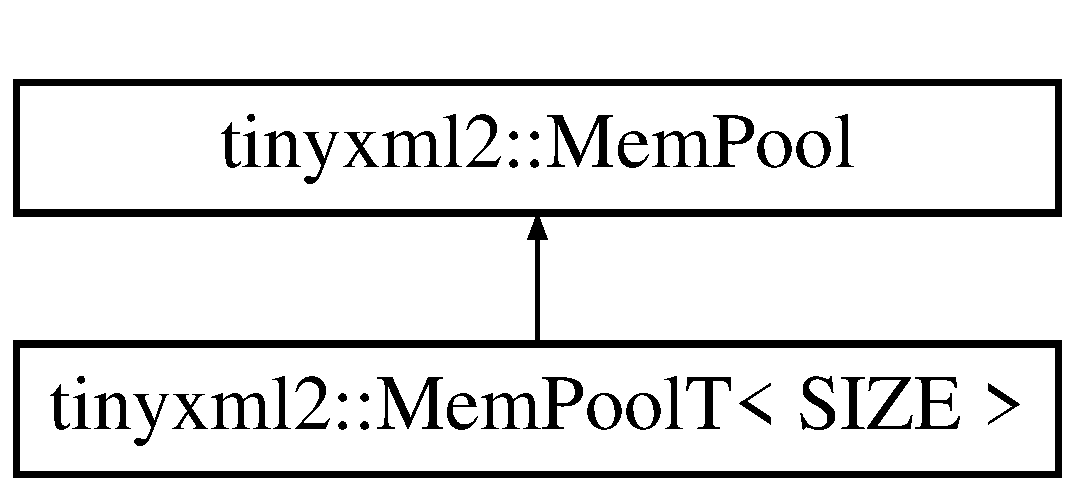
\includegraphics[height=2.000000cm]{classtinyxml2_1_1_mem_pool_t}
\end{center}
\end{figure}
\subsection*{Classes}
\begin{DoxyCompactItemize}
\item 
struct \hyperlink{structtinyxml2_1_1_mem_pool_t_1_1_block}{Block}
\item 
union \hyperlink{uniontinyxml2_1_1_mem_pool_t_1_1_chunk}{Chunk}
\end{DoxyCompactItemize}
\subsection*{Public Types}
\begin{DoxyCompactItemize}
\item 
enum \{ \hyperlink{classtinyxml2_1_1_mem_pool_t_a04cf45156e6f913f93972869ff8a1d94a4eeedbaa09fc9968120af6190e9e0988}{C\-O\-U\-N\-T} = (4$\ast$1024)/\-S\-I\-Z\-E
 \}
\end{DoxyCompactItemize}
\subsection*{Public Member Functions}
\begin{DoxyCompactItemize}
\item 
\hyperlink{classtinyxml2_1_1_mem_pool_t_a8a69a269ea72e292dde65309528ef64b}{Mem\-Pool\-T} ()
\item 
\hyperlink{classtinyxml2_1_1_mem_pool_t_ad6bb8346ad5b9a34f8f0051da5e3ed3f}{$\sim$\-Mem\-Pool\-T} ()
\item 
virtual int \hyperlink{classtinyxml2_1_1_mem_pool_t_a7ec8778fe99f6e332615a703be0b48bc}{Item\-Size} () const 
\item 
int \hyperlink{classtinyxml2_1_1_mem_pool_t_a56be11b7db6a7ef00db17088a7769aab}{Current\-Allocs} () const 
\item 
virtual void $\ast$ \hyperlink{classtinyxml2_1_1_mem_pool_t_aa9d785a48ffe6ea1be679bab13464486}{Alloc} ()
\item 
virtual void \hyperlink{classtinyxml2_1_1_mem_pool_t_a4f1a0c434e9e3d7391e5c16ed4ee8c70}{Free} (void $\ast$mem)
\item 
void \hyperlink{classtinyxml2_1_1_mem_pool_t_a0bc596f271e0f139822c534238b3f244}{Trace} (const char $\ast$name)
\item 
void \hyperlink{classtinyxml2_1_1_mem_pool_t_a7798932414916199a1bc0f9c3f368521}{Set\-Tracked} ()
\item 
int \hyperlink{classtinyxml2_1_1_mem_pool_t_a524b90d0edeac41964c06510757dce0f}{Untracked} () const 
\end{DoxyCompactItemize}
\subsection*{Private Attributes}
\begin{DoxyCompactItemize}
\item 
\hyperlink{classtinyxml2_1_1_dyn_array}{Dyn\-Array}$<$ \hyperlink{structtinyxml2_1_1_mem_pool_t_1_1_block}{Block} $\ast$, 10 $>$ \hyperlink{classtinyxml2_1_1_mem_pool_t_af8eeecccb8c484c34ba04e3757e081be}{\-\_\-block\-Ptrs}
\item 
\hyperlink{uniontinyxml2_1_1_mem_pool_t_1_1_chunk}{Chunk} $\ast$ \hyperlink{classtinyxml2_1_1_mem_pool_t_af203dc16256d7631fcbedd87864390bb}{\-\_\-root}
\item 
int \hyperlink{classtinyxml2_1_1_mem_pool_t_ae80f238a4c1fb0b2c037fd62b7bdd0c2}{\-\_\-current\-Allocs}
\item 
int \hyperlink{classtinyxml2_1_1_mem_pool_t_a1afde0bfad90d20643da123781664d7a}{\-\_\-n\-Allocs}
\item 
int \hyperlink{classtinyxml2_1_1_mem_pool_t_ac757df646660b4e8eefaca0d385f97dd}{\-\_\-max\-Allocs}
\item 
int \hyperlink{classtinyxml2_1_1_mem_pool_t_aca9adac3f7ce44a132dc00c285566b1e}{\-\_\-n\-Untracked}
\end{DoxyCompactItemize}


\subsection{Member Enumeration Documentation}
\hypertarget{classtinyxml2_1_1_mem_pool_t_a04cf45156e6f913f93972869ff8a1d94}{\subsubsection[{anonymous enum}]{\setlength{\rightskip}{0pt plus 5cm}template$<$int S\-I\-Z\-E$>$ anonymous enum}}\label{classtinyxml2_1_1_mem_pool_t_a04cf45156e6f913f93972869ff8a1d94}
\begin{Desc}
\item[Enumerator]\par
\begin{description}
\index{C\-O\-U\-N\-T@{C\-O\-U\-N\-T}!tinyxml2\-::\-Mem\-Pool\-T@{tinyxml2\-::\-Mem\-Pool\-T}}\index{tinyxml2\-::\-Mem\-Pool\-T@{tinyxml2\-::\-Mem\-Pool\-T}!C\-O\-U\-N\-T@{C\-O\-U\-N\-T}}\item[{\em 
\hypertarget{classtinyxml2_1_1_mem_pool_t_a04cf45156e6f913f93972869ff8a1d94a4eeedbaa09fc9968120af6190e9e0988}{C\-O\-U\-N\-T}\label{classtinyxml2_1_1_mem_pool_t_a04cf45156e6f913f93972869ff8a1d94a4eeedbaa09fc9968120af6190e9e0988}
}]\end{description}
\end{Desc}


\subsection{Constructor \& Destructor Documentation}
\hypertarget{classtinyxml2_1_1_mem_pool_t_a8a69a269ea72e292dde65309528ef64b}{\index{tinyxml2\-::\-Mem\-Pool\-T@{tinyxml2\-::\-Mem\-Pool\-T}!Mem\-Pool\-T@{Mem\-Pool\-T}}
\index{Mem\-Pool\-T@{Mem\-Pool\-T}!tinyxml2::MemPoolT@{tinyxml2\-::\-Mem\-Pool\-T}}
\subsubsection[{Mem\-Pool\-T}]{\setlength{\rightskip}{0pt plus 5cm}template$<$int S\-I\-Z\-E$>$ {\bf tinyxml2\-::\-Mem\-Pool\-T}$<$ S\-I\-Z\-E $>$\-::{\bf Mem\-Pool\-T} (
\begin{DoxyParamCaption}
{}
\end{DoxyParamCaption}
)\hspace{0.3cm}{\ttfamily [inline]}}}\label{classtinyxml2_1_1_mem_pool_t_a8a69a269ea72e292dde65309528ef64b}
\hypertarget{classtinyxml2_1_1_mem_pool_t_ad6bb8346ad5b9a34f8f0051da5e3ed3f}{\index{tinyxml2\-::\-Mem\-Pool\-T@{tinyxml2\-::\-Mem\-Pool\-T}!$\sim$\-Mem\-Pool\-T@{$\sim$\-Mem\-Pool\-T}}
\index{$\sim$\-Mem\-Pool\-T@{$\sim$\-Mem\-Pool\-T}!tinyxml2::MemPoolT@{tinyxml2\-::\-Mem\-Pool\-T}}
\subsubsection[{$\sim$\-Mem\-Pool\-T}]{\setlength{\rightskip}{0pt plus 5cm}template$<$int S\-I\-Z\-E$>$ {\bf tinyxml2\-::\-Mem\-Pool\-T}$<$ S\-I\-Z\-E $>$\-::$\sim${\bf Mem\-Pool\-T} (
\begin{DoxyParamCaption}
{}
\end{DoxyParamCaption}
)\hspace{0.3cm}{\ttfamily [inline]}}}\label{classtinyxml2_1_1_mem_pool_t_ad6bb8346ad5b9a34f8f0051da5e3ed3f}


\subsection{Member Function Documentation}
\hypertarget{classtinyxml2_1_1_mem_pool_t_aa9d785a48ffe6ea1be679bab13464486}{\index{tinyxml2\-::\-Mem\-Pool\-T@{tinyxml2\-::\-Mem\-Pool\-T}!Alloc@{Alloc}}
\index{Alloc@{Alloc}!tinyxml2::MemPoolT@{tinyxml2\-::\-Mem\-Pool\-T}}
\subsubsection[{Alloc}]{\setlength{\rightskip}{0pt plus 5cm}template$<$int S\-I\-Z\-E$>$ virtual void$\ast$ {\bf tinyxml2\-::\-Mem\-Pool\-T}$<$ S\-I\-Z\-E $>$\-::Alloc (
\begin{DoxyParamCaption}
{}
\end{DoxyParamCaption}
)\hspace{0.3cm}{\ttfamily [inline]}, {\ttfamily [virtual]}}}\label{classtinyxml2_1_1_mem_pool_t_aa9d785a48ffe6ea1be679bab13464486}


Implements \hyperlink{classtinyxml2_1_1_mem_pool_a4f977b5fed752c0bbfe5295f469d6449}{tinyxml2\-::\-Mem\-Pool}.

\hypertarget{classtinyxml2_1_1_mem_pool_t_a56be11b7db6a7ef00db17088a7769aab}{\index{tinyxml2\-::\-Mem\-Pool\-T@{tinyxml2\-::\-Mem\-Pool\-T}!Current\-Allocs@{Current\-Allocs}}
\index{Current\-Allocs@{Current\-Allocs}!tinyxml2::MemPoolT@{tinyxml2\-::\-Mem\-Pool\-T}}
\subsubsection[{Current\-Allocs}]{\setlength{\rightskip}{0pt plus 5cm}template$<$int S\-I\-Z\-E$>$ int {\bf tinyxml2\-::\-Mem\-Pool\-T}$<$ S\-I\-Z\-E $>$\-::Current\-Allocs (
\begin{DoxyParamCaption}
{}
\end{DoxyParamCaption}
) const\hspace{0.3cm}{\ttfamily [inline]}}}\label{classtinyxml2_1_1_mem_pool_t_a56be11b7db6a7ef00db17088a7769aab}
\hypertarget{classtinyxml2_1_1_mem_pool_t_a4f1a0c434e9e3d7391e5c16ed4ee8c70}{\index{tinyxml2\-::\-Mem\-Pool\-T@{tinyxml2\-::\-Mem\-Pool\-T}!Free@{Free}}
\index{Free@{Free}!tinyxml2::MemPoolT@{tinyxml2\-::\-Mem\-Pool\-T}}
\subsubsection[{Free}]{\setlength{\rightskip}{0pt plus 5cm}template$<$int S\-I\-Z\-E$>$ virtual void {\bf tinyxml2\-::\-Mem\-Pool\-T}$<$ S\-I\-Z\-E $>$\-::Free (
\begin{DoxyParamCaption}
\item[{void $\ast$}]{mem}
\end{DoxyParamCaption}
)\hspace{0.3cm}{\ttfamily [inline]}, {\ttfamily [virtual]}}}\label{classtinyxml2_1_1_mem_pool_t_a4f1a0c434e9e3d7391e5c16ed4ee8c70}


Implements \hyperlink{classtinyxml2_1_1_mem_pool_a49e3bfac2cba2ebd6776b31e571f64f7}{tinyxml2\-::\-Mem\-Pool}.

\hypertarget{classtinyxml2_1_1_mem_pool_t_a7ec8778fe99f6e332615a703be0b48bc}{\index{tinyxml2\-::\-Mem\-Pool\-T@{tinyxml2\-::\-Mem\-Pool\-T}!Item\-Size@{Item\-Size}}
\index{Item\-Size@{Item\-Size}!tinyxml2::MemPoolT@{tinyxml2\-::\-Mem\-Pool\-T}}
\subsubsection[{Item\-Size}]{\setlength{\rightskip}{0pt plus 5cm}template$<$int S\-I\-Z\-E$>$ virtual int {\bf tinyxml2\-::\-Mem\-Pool\-T}$<$ S\-I\-Z\-E $>$\-::Item\-Size (
\begin{DoxyParamCaption}
{}
\end{DoxyParamCaption}
) const\hspace{0.3cm}{\ttfamily [inline]}, {\ttfamily [virtual]}}}\label{classtinyxml2_1_1_mem_pool_t_a7ec8778fe99f6e332615a703be0b48bc}


Implements \hyperlink{classtinyxml2_1_1_mem_pool_a0c518d49e3a94bde566f61e13b7240bb}{tinyxml2\-::\-Mem\-Pool}.

\hypertarget{classtinyxml2_1_1_mem_pool_t_a7798932414916199a1bc0f9c3f368521}{\index{tinyxml2\-::\-Mem\-Pool\-T@{tinyxml2\-::\-Mem\-Pool\-T}!Set\-Tracked@{Set\-Tracked}}
\index{Set\-Tracked@{Set\-Tracked}!tinyxml2::MemPoolT@{tinyxml2\-::\-Mem\-Pool\-T}}
\subsubsection[{Set\-Tracked}]{\setlength{\rightskip}{0pt plus 5cm}template$<$int S\-I\-Z\-E$>$ void {\bf tinyxml2\-::\-Mem\-Pool\-T}$<$ S\-I\-Z\-E $>$\-::Set\-Tracked (
\begin{DoxyParamCaption}
{}
\end{DoxyParamCaption}
)\hspace{0.3cm}{\ttfamily [inline]}, {\ttfamily [virtual]}}}\label{classtinyxml2_1_1_mem_pool_t_a7798932414916199a1bc0f9c3f368521}


Implements \hyperlink{classtinyxml2_1_1_mem_pool_ac5804dd1387b2e4de5eef710076a0db1}{tinyxml2\-::\-Mem\-Pool}.

\hypertarget{classtinyxml2_1_1_mem_pool_t_a0bc596f271e0f139822c534238b3f244}{\index{tinyxml2\-::\-Mem\-Pool\-T@{tinyxml2\-::\-Mem\-Pool\-T}!Trace@{Trace}}
\index{Trace@{Trace}!tinyxml2::MemPoolT@{tinyxml2\-::\-Mem\-Pool\-T}}
\subsubsection[{Trace}]{\setlength{\rightskip}{0pt plus 5cm}template$<$int S\-I\-Z\-E$>$ void {\bf tinyxml2\-::\-Mem\-Pool\-T}$<$ S\-I\-Z\-E $>$\-::Trace (
\begin{DoxyParamCaption}
\item[{const char $\ast$}]{name}
\end{DoxyParamCaption}
)\hspace{0.3cm}{\ttfamily [inline]}}}\label{classtinyxml2_1_1_mem_pool_t_a0bc596f271e0f139822c534238b3f244}
\hypertarget{classtinyxml2_1_1_mem_pool_t_a524b90d0edeac41964c06510757dce0f}{\index{tinyxml2\-::\-Mem\-Pool\-T@{tinyxml2\-::\-Mem\-Pool\-T}!Untracked@{Untracked}}
\index{Untracked@{Untracked}!tinyxml2::MemPoolT@{tinyxml2\-::\-Mem\-Pool\-T}}
\subsubsection[{Untracked}]{\setlength{\rightskip}{0pt plus 5cm}template$<$int S\-I\-Z\-E$>$ int {\bf tinyxml2\-::\-Mem\-Pool\-T}$<$ S\-I\-Z\-E $>$\-::Untracked (
\begin{DoxyParamCaption}
{}
\end{DoxyParamCaption}
) const\hspace{0.3cm}{\ttfamily [inline]}}}\label{classtinyxml2_1_1_mem_pool_t_a524b90d0edeac41964c06510757dce0f}


\subsection{Member Data Documentation}
\hypertarget{classtinyxml2_1_1_mem_pool_t_af8eeecccb8c484c34ba04e3757e081be}{\index{tinyxml2\-::\-Mem\-Pool\-T@{tinyxml2\-::\-Mem\-Pool\-T}!\-\_\-block\-Ptrs@{\-\_\-block\-Ptrs}}
\index{\-\_\-block\-Ptrs@{\-\_\-block\-Ptrs}!tinyxml2::MemPoolT@{tinyxml2\-::\-Mem\-Pool\-T}}
\subsubsection[{\-\_\-block\-Ptrs}]{\setlength{\rightskip}{0pt plus 5cm}template$<$int S\-I\-Z\-E$>$ {\bf Dyn\-Array}$<$ {\bf Block}$\ast$, 10 $>$ {\bf tinyxml2\-::\-Mem\-Pool\-T}$<$ S\-I\-Z\-E $>$\-::\-\_\-block\-Ptrs\hspace{0.3cm}{\ttfamily [private]}}}\label{classtinyxml2_1_1_mem_pool_t_af8eeecccb8c484c34ba04e3757e081be}
\hypertarget{classtinyxml2_1_1_mem_pool_t_ae80f238a4c1fb0b2c037fd62b7bdd0c2}{\index{tinyxml2\-::\-Mem\-Pool\-T@{tinyxml2\-::\-Mem\-Pool\-T}!\-\_\-current\-Allocs@{\-\_\-current\-Allocs}}
\index{\-\_\-current\-Allocs@{\-\_\-current\-Allocs}!tinyxml2::MemPoolT@{tinyxml2\-::\-Mem\-Pool\-T}}
\subsubsection[{\-\_\-current\-Allocs}]{\setlength{\rightskip}{0pt plus 5cm}template$<$int S\-I\-Z\-E$>$ int {\bf tinyxml2\-::\-Mem\-Pool\-T}$<$ S\-I\-Z\-E $>$\-::\-\_\-current\-Allocs\hspace{0.3cm}{\ttfamily [private]}}}\label{classtinyxml2_1_1_mem_pool_t_ae80f238a4c1fb0b2c037fd62b7bdd0c2}
\hypertarget{classtinyxml2_1_1_mem_pool_t_ac757df646660b4e8eefaca0d385f97dd}{\index{tinyxml2\-::\-Mem\-Pool\-T@{tinyxml2\-::\-Mem\-Pool\-T}!\-\_\-max\-Allocs@{\-\_\-max\-Allocs}}
\index{\-\_\-max\-Allocs@{\-\_\-max\-Allocs}!tinyxml2::MemPoolT@{tinyxml2\-::\-Mem\-Pool\-T}}
\subsubsection[{\-\_\-max\-Allocs}]{\setlength{\rightskip}{0pt plus 5cm}template$<$int S\-I\-Z\-E$>$ int {\bf tinyxml2\-::\-Mem\-Pool\-T}$<$ S\-I\-Z\-E $>$\-::\-\_\-max\-Allocs\hspace{0.3cm}{\ttfamily [private]}}}\label{classtinyxml2_1_1_mem_pool_t_ac757df646660b4e8eefaca0d385f97dd}
\hypertarget{classtinyxml2_1_1_mem_pool_t_a1afde0bfad90d20643da123781664d7a}{\index{tinyxml2\-::\-Mem\-Pool\-T@{tinyxml2\-::\-Mem\-Pool\-T}!\-\_\-n\-Allocs@{\-\_\-n\-Allocs}}
\index{\-\_\-n\-Allocs@{\-\_\-n\-Allocs}!tinyxml2::MemPoolT@{tinyxml2\-::\-Mem\-Pool\-T}}
\subsubsection[{\-\_\-n\-Allocs}]{\setlength{\rightskip}{0pt plus 5cm}template$<$int S\-I\-Z\-E$>$ int {\bf tinyxml2\-::\-Mem\-Pool\-T}$<$ S\-I\-Z\-E $>$\-::\-\_\-n\-Allocs\hspace{0.3cm}{\ttfamily [private]}}}\label{classtinyxml2_1_1_mem_pool_t_a1afde0bfad90d20643da123781664d7a}
\hypertarget{classtinyxml2_1_1_mem_pool_t_aca9adac3f7ce44a132dc00c285566b1e}{\index{tinyxml2\-::\-Mem\-Pool\-T@{tinyxml2\-::\-Mem\-Pool\-T}!\-\_\-n\-Untracked@{\-\_\-n\-Untracked}}
\index{\-\_\-n\-Untracked@{\-\_\-n\-Untracked}!tinyxml2::MemPoolT@{tinyxml2\-::\-Mem\-Pool\-T}}
\subsubsection[{\-\_\-n\-Untracked}]{\setlength{\rightskip}{0pt plus 5cm}template$<$int S\-I\-Z\-E$>$ int {\bf tinyxml2\-::\-Mem\-Pool\-T}$<$ S\-I\-Z\-E $>$\-::\-\_\-n\-Untracked\hspace{0.3cm}{\ttfamily [private]}}}\label{classtinyxml2_1_1_mem_pool_t_aca9adac3f7ce44a132dc00c285566b1e}
\hypertarget{classtinyxml2_1_1_mem_pool_t_af203dc16256d7631fcbedd87864390bb}{\index{tinyxml2\-::\-Mem\-Pool\-T@{tinyxml2\-::\-Mem\-Pool\-T}!\-\_\-root@{\-\_\-root}}
\index{\-\_\-root@{\-\_\-root}!tinyxml2::MemPoolT@{tinyxml2\-::\-Mem\-Pool\-T}}
\subsubsection[{\-\_\-root}]{\setlength{\rightskip}{0pt plus 5cm}template$<$int S\-I\-Z\-E$>$ {\bf Chunk}$\ast$ {\bf tinyxml2\-::\-Mem\-Pool\-T}$<$ S\-I\-Z\-E $>$\-::\-\_\-root\hspace{0.3cm}{\ttfamily [private]}}}\label{classtinyxml2_1_1_mem_pool_t_af203dc16256d7631fcbedd87864390bb}


The documentation for this class was generated from the following file\-:\begin{DoxyCompactItemize}
\item 
Utils/\-X\-M\-L\-\_\-\-Config/\hyperlink{tinyxml2_8h}{tinyxml2.\-h}\end{DoxyCompactItemize}

\hypertarget{classn8_1_1_music}{\section{n8\-:\-:Music Class Reference}
\label{classn8_1_1_music}\index{n8\-::\-Music@{n8\-::\-Music}}
}


{\ttfamily \#include $<$Music.\-h$>$}

Inheritance diagram for n8\-:\-:Music\-:\begin{figure}[H]
\begin{center}
\leavevmode
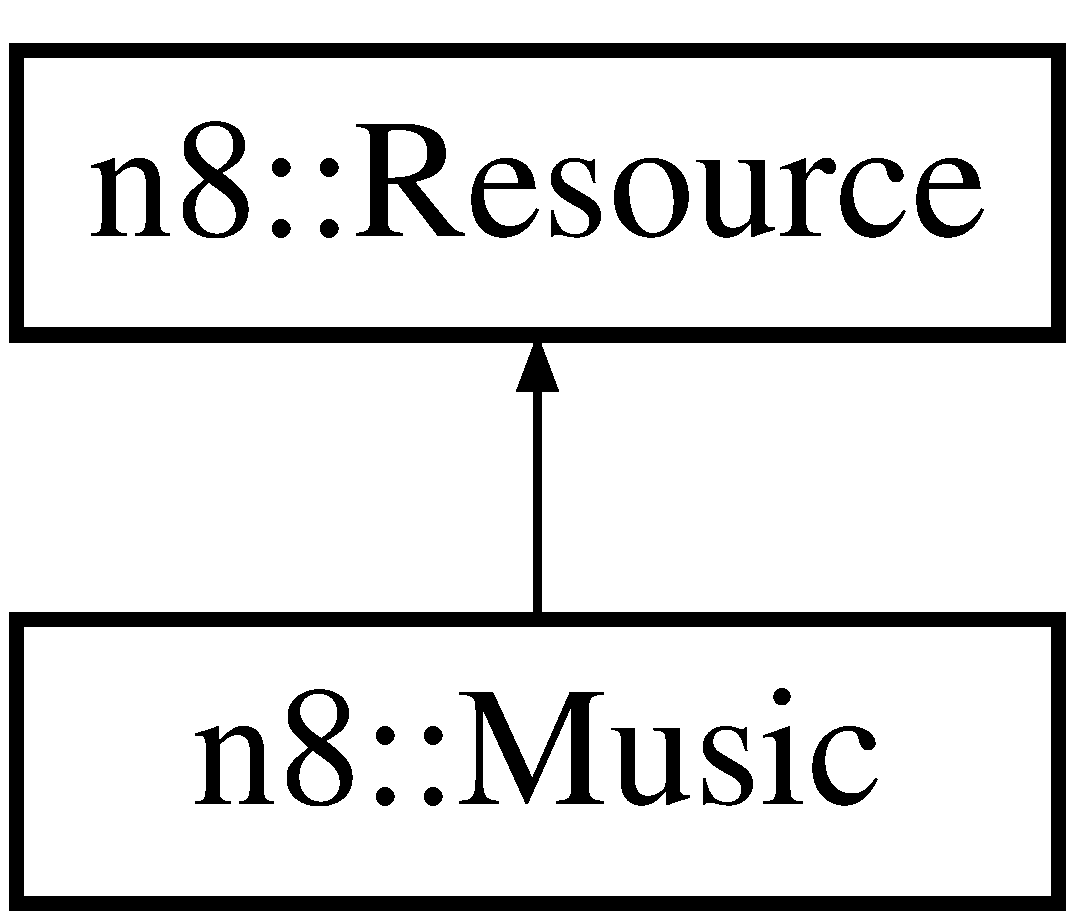
\includegraphics[height=2.000000cm]{classn8_1_1_music}
\end{center}
\end{figure}
\subsection*{Public Member Functions}
\begin{DoxyCompactItemize}
\item 
\hyperlink{classn8_1_1_music_a6f7b8099e92cc93cfdde874cc9974576}{Music} (std\-::string p\-\_\-id, Mix\-\_\-\-Music $\ast$p\-\_\-mix\-Music)
\item 
\hyperlink{classn8_1_1_music_a3953e196b66bd023d77930fa7feb48cf}{$\sim$\-Music} ()
\end{DoxyCompactItemize}
\subsection*{Private Attributes}
\begin{DoxyCompactItemize}
\item 
Mix\-\_\-\-Music $\ast$ \hyperlink{classn8_1_1_music_a9189b4b9d590b9d8adb49d793cede1b4}{m\-\_\-music}
\end{DoxyCompactItemize}
\subsection*{Friends}
\begin{DoxyCompactItemize}
\item 
class \hyperlink{classn8_1_1_music_a37b580cb33a7b41e459ef8adf3e2dd75}{Audio\-Service}
\end{DoxyCompactItemize}


\subsection{Constructor \& Destructor Documentation}
\hypertarget{classn8_1_1_music_a6f7b8099e92cc93cfdde874cc9974576}{\index{n8\-::\-Music@{n8\-::\-Music}!Music@{Music}}
\index{Music@{Music}!n8::Music@{n8\-::\-Music}}
\subsubsection[{Music}]{\setlength{\rightskip}{0pt plus 5cm}n8\-::\-Music\-::\-Music (
\begin{DoxyParamCaption}
\item[{std\-::string}]{p\-\_\-id, }
\item[{Mix\-\_\-\-Music $\ast$}]{p\-\_\-mix\-Music}
\end{DoxyParamCaption}
)}}\label{classn8_1_1_music_a6f7b8099e92cc93cfdde874cc9974576}
\hypertarget{classn8_1_1_music_a3953e196b66bd023d77930fa7feb48cf}{\index{n8\-::\-Music@{n8\-::\-Music}!$\sim$\-Music@{$\sim$\-Music}}
\index{$\sim$\-Music@{$\sim$\-Music}!n8::Music@{n8\-::\-Music}}
\subsubsection[{$\sim$\-Music}]{\setlength{\rightskip}{0pt plus 5cm}n8\-::\-Music\-::$\sim$\-Music (
\begin{DoxyParamCaption}
{}
\end{DoxyParamCaption}
)}}\label{classn8_1_1_music_a3953e196b66bd023d77930fa7feb48cf}


\subsection{Friends And Related Function Documentation}
\hypertarget{classn8_1_1_music_a37b580cb33a7b41e459ef8adf3e2dd75}{\index{n8\-::\-Music@{n8\-::\-Music}!Audio\-Service@{Audio\-Service}}
\index{Audio\-Service@{Audio\-Service}!n8::Music@{n8\-::\-Music}}
\subsubsection[{Audio\-Service}]{\setlength{\rightskip}{0pt plus 5cm}friend class Audio\-Service\hspace{0.3cm}{\ttfamily [friend]}}}\label{classn8_1_1_music_a37b580cb33a7b41e459ef8adf3e2dd75}


\subsection{Member Data Documentation}
\hypertarget{classn8_1_1_music_a9189b4b9d590b9d8adb49d793cede1b4}{\index{n8\-::\-Music@{n8\-::\-Music}!m\-\_\-music@{m\-\_\-music}}
\index{m\-\_\-music@{m\-\_\-music}!n8::Music@{n8\-::\-Music}}
\subsubsection[{m\-\_\-music}]{\setlength{\rightskip}{0pt plus 5cm}Mix\-\_\-\-Music$\ast$ n8\-::\-Music\-::m\-\_\-music\hspace{0.3cm}{\ttfamily [private]}}}\label{classn8_1_1_music_a9189b4b9d590b9d8adb49d793cede1b4}


The documentation for this class was generated from the following files\-:\begin{DoxyCompactItemize}
\item 
Resources/\hyperlink{_music_8h}{Music.\-h}\item 
Resources/\hyperlink{_music_8cpp}{Music.\-cpp}\end{DoxyCompactItemize}

\hypertarget{classn8_1_1_object_factory}{\section{n8\-:\-:Object\-Factory Class Reference}
\label{classn8_1_1_object_factory}\index{n8\-::\-Object\-Factory@{n8\-::\-Object\-Factory}}
}


{\ttfamily \#include $<$Object\-Factory.\-h$>$}

\subsection*{Public Member Functions}
\begin{DoxyCompactItemize}
\item 
\hyperlink{classn8_1_1_object_factory_a0da24c26e7ece19314ede4d785bbace0}{Object\-Factory} ()
\item 
virtual \hyperlink{classn8_1_1_object_factory_adfdbda35f6b0f3a3cc1bc224f4712c03}{$\sim$\-Object\-Factory} ()=0
\item 
int \hyperlink{classn8_1_1_object_factory_a1f79e646d459d001f62f1920c323e204}{Get\-Next\-Id} ()
\end{DoxyCompactItemize}
\subsection*{Static Public Attributes}
\begin{DoxyCompactItemize}
\item 
static int \hyperlink{classn8_1_1_object_factory_af9e6c6cb3ab18962dfa4859ceb289923}{m\-\_\-next\-Id} = 0
\end{DoxyCompactItemize}


\subsection{Constructor \& Destructor Documentation}
\hypertarget{classn8_1_1_object_factory_a0da24c26e7ece19314ede4d785bbace0}{\index{n8\-::\-Object\-Factory@{n8\-::\-Object\-Factory}!Object\-Factory@{Object\-Factory}}
\index{Object\-Factory@{Object\-Factory}!n8::ObjectFactory@{n8\-::\-Object\-Factory}}
\subsubsection[{Object\-Factory}]{\setlength{\rightskip}{0pt plus 5cm}n8\-::\-Object\-Factory\-::\-Object\-Factory (
\begin{DoxyParamCaption}
{}
\end{DoxyParamCaption}
)}}\label{classn8_1_1_object_factory_a0da24c26e7ece19314ede4d785bbace0}
$<$ Static counter to get available id values for created entities \hypertarget{classn8_1_1_object_factory_adfdbda35f6b0f3a3cc1bc224f4712c03}{\index{n8\-::\-Object\-Factory@{n8\-::\-Object\-Factory}!$\sim$\-Object\-Factory@{$\sim$\-Object\-Factory}}
\index{$\sim$\-Object\-Factory@{$\sim$\-Object\-Factory}!n8::ObjectFactory@{n8\-::\-Object\-Factory}}
\subsubsection[{$\sim$\-Object\-Factory}]{\setlength{\rightskip}{0pt plus 5cm}virtual n8\-::\-Object\-Factory\-::$\sim$\-Object\-Factory (
\begin{DoxyParamCaption}
{}
\end{DoxyParamCaption}
)\hspace{0.3cm}{\ttfamily [pure virtual]}}}\label{classn8_1_1_object_factory_adfdbda35f6b0f3a3cc1bc224f4712c03}


\subsection{Member Function Documentation}
\hypertarget{classn8_1_1_object_factory_a1f79e646d459d001f62f1920c323e204}{\index{n8\-::\-Object\-Factory@{n8\-::\-Object\-Factory}!Get\-Next\-Id@{Get\-Next\-Id}}
\index{Get\-Next\-Id@{Get\-Next\-Id}!n8::ObjectFactory@{n8\-::\-Object\-Factory}}
\subsubsection[{Get\-Next\-Id}]{\setlength{\rightskip}{0pt plus 5cm}int n8\-::\-Object\-Factory\-::\-Get\-Next\-Id (
\begin{DoxyParamCaption}
{}
\end{DoxyParamCaption}
)}}\label{classn8_1_1_object_factory_a1f79e646d459d001f62f1920c323e204}
Used to get the next available unique integer id for a created entity. When called nextid\-\_\- is incremented so the return values are always unique.

\begin{DoxyReturn}{Returns}
The next available id number 
\end{DoxyReturn}


\subsection{Member Data Documentation}
\hypertarget{classn8_1_1_object_factory_af9e6c6cb3ab18962dfa4859ceb289923}{\index{n8\-::\-Object\-Factory@{n8\-::\-Object\-Factory}!m\-\_\-next\-Id@{m\-\_\-next\-Id}}
\index{m\-\_\-next\-Id@{m\-\_\-next\-Id}!n8::ObjectFactory@{n8\-::\-Object\-Factory}}
\subsubsection[{m\-\_\-next\-Id}]{\setlength{\rightskip}{0pt plus 5cm}int n8\-::\-Object\-Factory\-::m\-\_\-next\-Id = 0\hspace{0.3cm}{\ttfamily [static]}}}\label{classn8_1_1_object_factory_af9e6c6cb3ab18962dfa4859ceb289923}


The documentation for this class was generated from the following files\-:\begin{DoxyCompactItemize}
\item 
Base/\hyperlink{_object_factory_8h}{Object\-Factory.\-h}\item 
Base/\hyperlink{_object_factory_8cpp}{Object\-Factory.\-cpp}\end{DoxyCompactItemize}

\hypertarget{classn8_1_1_observer}{\section{n8\-:\-:Observer Class Reference}
\label{classn8_1_1_observer}\index{n8\-::\-Observer@{n8\-::\-Observer}}
}


{\ttfamily \#include $<$Observer.\-h$>$}

Inheritance diagram for n8\-:\-:Observer\-:\begin{figure}[H]
\begin{center}
\leavevmode
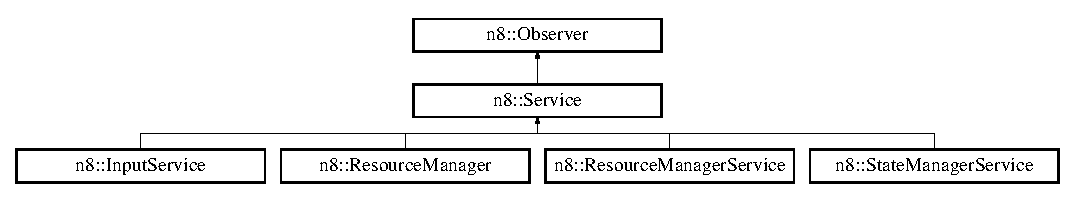
\includegraphics[height=2.222222cm]{classn8_1_1_observer}
\end{center}
\end{figure}
\subsection*{Public Member Functions}
\begin{DoxyCompactItemize}
\item 
virtual \hyperlink{classn8_1_1_observer_a23559325d1772eba6928c160d5b8853b}{$\sim$\-Observer} ()
\item 
virtual void \hyperlink{classn8_1_1_observer_ab08ada5adb0e21dbb2ee30c26652fd32}{On\-Notify} (\hyperlink{classn8_1_1_event}{Event} $\ast$event)=0
\end{DoxyCompactItemize}


\subsection{Detailed Description}
Class to allow events to be handled in an uncoupled manner. Follows the common \hyperlink{classn8_1_1_observer}{Observer} design pattern. 

\subsection{Constructor \& Destructor Documentation}
\hypertarget{classn8_1_1_observer_a23559325d1772eba6928c160d5b8853b}{\index{n8\-::\-Observer@{n8\-::\-Observer}!$\sim$\-Observer@{$\sim$\-Observer}}
\index{$\sim$\-Observer@{$\sim$\-Observer}!n8::Observer@{n8\-::\-Observer}}
\subsubsection[{$\sim$\-Observer}]{\setlength{\rightskip}{0pt plus 5cm}virtual n8\-::\-Observer\-::$\sim$\-Observer (
\begin{DoxyParamCaption}
{}
\end{DoxyParamCaption}
)\hspace{0.3cm}{\ttfamily [inline]}, {\ttfamily [virtual]}}}\label{classn8_1_1_observer_a23559325d1772eba6928c160d5b8853b}


\subsection{Member Function Documentation}
\hypertarget{classn8_1_1_observer_ab08ada5adb0e21dbb2ee30c26652fd32}{\index{n8\-::\-Observer@{n8\-::\-Observer}!On\-Notify@{On\-Notify}}
\index{On\-Notify@{On\-Notify}!n8::Observer@{n8\-::\-Observer}}
\subsubsection[{On\-Notify}]{\setlength{\rightskip}{0pt plus 5cm}virtual void n8\-::\-Observer\-::\-On\-Notify (
\begin{DoxyParamCaption}
\item[{{\bf Event} $\ast$}]{event}
\end{DoxyParamCaption}
)\hspace{0.3cm}{\ttfamily [pure virtual]}}}\label{classn8_1_1_observer_ab08ada5adb0e21dbb2ee30c26652fd32}


Implemented in \hyperlink{classn8_1_1_resource_manager_ace97033b439ac0954cf2fc45a79081c9}{n8\-::\-Resource\-Manager}, \hyperlink{classn8_1_1_state_manager_service_a931551f9b6dc470297e9d86abf27b603}{n8\-::\-State\-Manager\-Service}, \hyperlink{classn8_1_1_input_service_aa52767bfd35d3785ea236c8175598212}{n8\-::\-Input\-Service}, \hyperlink{classn8_1_1_resource_manager_service_a0c5bb1ec14fea9971e8fec2efe8d56cd}{n8\-::\-Resource\-Manager\-Service}, and \hyperlink{classn8_1_1_service_a756a170eba7e5c34a1c12008e22d3ca7}{n8\-::\-Service}.



The documentation for this class was generated from the following file\-:\begin{DoxyCompactItemize}
\item 
Communication/\hyperlink{_observer_8h}{Observer.\-h}\end{DoxyCompactItemize}

\hypertarget{classn8_1_1_pop_state_command}{\section{n8\-:\-:Pop\-State\-Command Class Reference}
\label{classn8_1_1_pop_state_command}\index{n8\-::\-Pop\-State\-Command@{n8\-::\-Pop\-State\-Command}}
}


{\ttfamily \#include $<$Pop\-State\-Command.\-h$>$}

Inheritance diagram for n8\-:\-:Pop\-State\-Command\-:\begin{figure}[H]
\begin{center}
\leavevmode
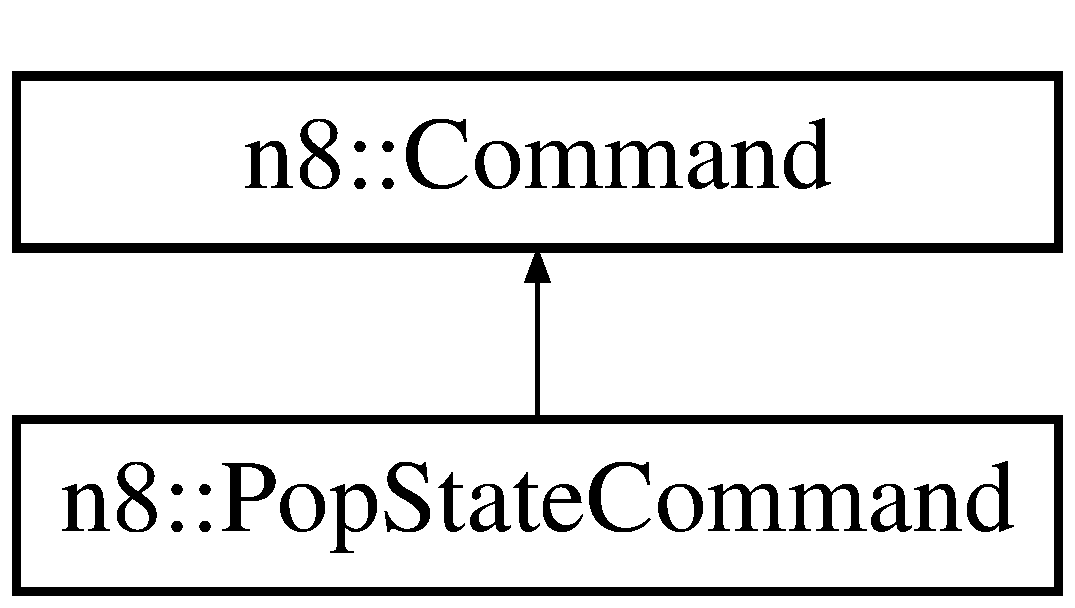
\includegraphics[height=2.000000cm]{classn8_1_1_pop_state_command}
\end{center}
\end{figure}
\subsection*{Public Member Functions}
\begin{DoxyCompactItemize}
\item 
\hyperlink{classn8_1_1_pop_state_command_a030daf82728757ac8124fa7d5bea5a9c}{Pop\-State\-Command} ()
\item 
\hyperlink{classn8_1_1_pop_state_command_a9cca8868fb822f469c4bcfec426a6963}{$\sim$\-Pop\-State\-Command} ()
\item 
virtual void \hyperlink{classn8_1_1_pop_state_command_aa17a7fa17704fe0ba20dcebde250e19b}{execute} ()
\end{DoxyCompactItemize}


\subsection{Constructor \& Destructor Documentation}
\hypertarget{classn8_1_1_pop_state_command_a030daf82728757ac8124fa7d5bea5a9c}{\index{n8\-::\-Pop\-State\-Command@{n8\-::\-Pop\-State\-Command}!Pop\-State\-Command@{Pop\-State\-Command}}
\index{Pop\-State\-Command@{Pop\-State\-Command}!n8::PopStateCommand@{n8\-::\-Pop\-State\-Command}}
\subsubsection[{Pop\-State\-Command}]{\setlength{\rightskip}{0pt plus 5cm}n8\-::\-Pop\-State\-Command\-::\-Pop\-State\-Command (
\begin{DoxyParamCaption}
{}
\end{DoxyParamCaption}
)}}\label{classn8_1_1_pop_state_command_a030daf82728757ac8124fa7d5bea5a9c}
\hypertarget{classn8_1_1_pop_state_command_a9cca8868fb822f469c4bcfec426a6963}{\index{n8\-::\-Pop\-State\-Command@{n8\-::\-Pop\-State\-Command}!$\sim$\-Pop\-State\-Command@{$\sim$\-Pop\-State\-Command}}
\index{$\sim$\-Pop\-State\-Command@{$\sim$\-Pop\-State\-Command}!n8::PopStateCommand@{n8\-::\-Pop\-State\-Command}}
\subsubsection[{$\sim$\-Pop\-State\-Command}]{\setlength{\rightskip}{0pt plus 5cm}n8\-::\-Pop\-State\-Command\-::$\sim$\-Pop\-State\-Command (
\begin{DoxyParamCaption}
{}
\end{DoxyParamCaption}
)}}\label{classn8_1_1_pop_state_command_a9cca8868fb822f469c4bcfec426a6963}


\subsection{Member Function Documentation}
\hypertarget{classn8_1_1_pop_state_command_aa17a7fa17704fe0ba20dcebde250e19b}{\index{n8\-::\-Pop\-State\-Command@{n8\-::\-Pop\-State\-Command}!execute@{execute}}
\index{execute@{execute}!n8::PopStateCommand@{n8\-::\-Pop\-State\-Command}}
\subsubsection[{execute}]{\setlength{\rightskip}{0pt plus 5cm}void n8\-::\-Pop\-State\-Command\-::execute (
\begin{DoxyParamCaption}
{}
\end{DoxyParamCaption}
)\hspace{0.3cm}{\ttfamily [virtual]}}}\label{classn8_1_1_pop_state_command_aa17a7fa17704fe0ba20dcebde250e19b}


Implements \hyperlink{classn8_1_1_command_a8a70ef93c997ef2f545154e1c55cdf87}{n8\-::\-Command}.



The documentation for this class was generated from the following files\-:\begin{DoxyCompactItemize}
\item 
Commands/\hyperlink{_pop_state_command_8h}{Pop\-State\-Command.\-h}\item 
Commands/\hyperlink{_pop_state_command_8cpp}{Pop\-State\-Command.\-cpp}\end{DoxyCompactItemize}

\hypertarget{classn8_1_1_push_state_command}{\section{n8\-:\-:Push\-State\-Command Class Reference}
\label{classn8_1_1_push_state_command}\index{n8\-::\-Push\-State\-Command@{n8\-::\-Push\-State\-Command}}
}


{\ttfamily \#include $<$Push\-State\-Command.\-h$>$}

Inheritance diagram for n8\-:\-:Push\-State\-Command\-:\begin{figure}[H]
\begin{center}
\leavevmode
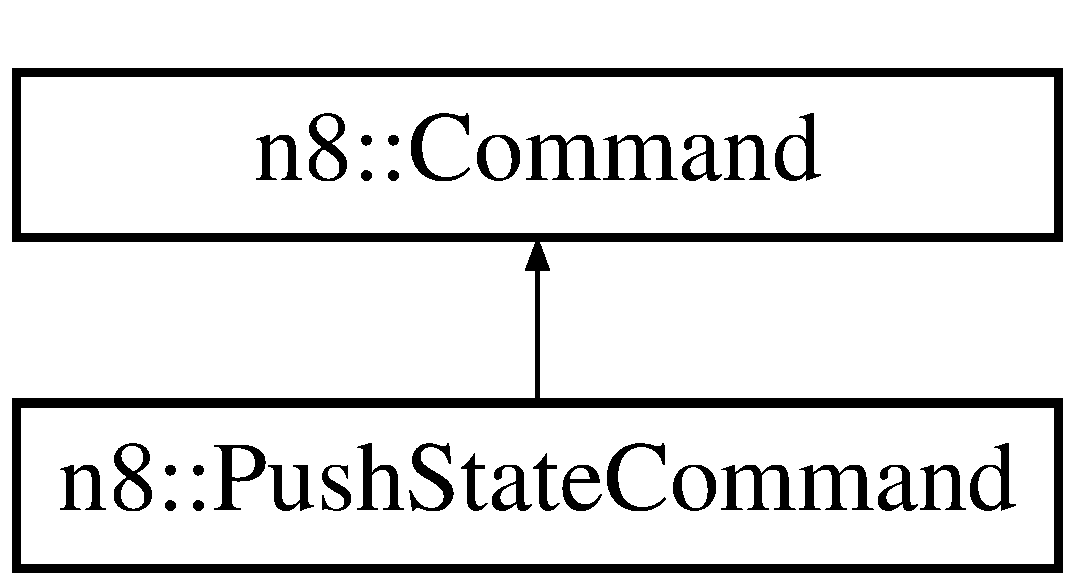
\includegraphics[height=2.000000cm]{classn8_1_1_push_state_command}
\end{center}
\end{figure}
\subsection*{Public Member Functions}
\begin{DoxyCompactItemize}
\item 
\hyperlink{classn8_1_1_push_state_command_ae1c85b830260a6d29cf6f6d4730559ff}{Push\-State\-Command} (\hyperlink{namespace_e_state_aee586325ec9fecd1205d41439870dd81}{E\-State\-::\-Values})
\item 
\hyperlink{classn8_1_1_push_state_command_ab593c046bb4361ebae9a311dafe5a30b}{$\sim$\-Push\-State\-Command} ()
\item 
virtual void \hyperlink{classn8_1_1_push_state_command_ab3019fecfe1aee633c6d3b3cf68f2e70}{execute} ()
\end{DoxyCompactItemize}
\subsection*{Private Attributes}
\begin{DoxyCompactItemize}
\item 
\hyperlink{namespace_e_state_aee586325ec9fecd1205d41439870dd81}{E\-State\-::\-Values} \hyperlink{classn8_1_1_push_state_command_abd110a1cf9efc34960652d3aa90e4828}{m\-\_\-state}
\end{DoxyCompactItemize}


\subsection{Constructor \& Destructor Documentation}
\hypertarget{classn8_1_1_push_state_command_ae1c85b830260a6d29cf6f6d4730559ff}{\index{n8\-::\-Push\-State\-Command@{n8\-::\-Push\-State\-Command}!Push\-State\-Command@{Push\-State\-Command}}
\index{Push\-State\-Command@{Push\-State\-Command}!n8::PushStateCommand@{n8\-::\-Push\-State\-Command}}
\subsubsection[{Push\-State\-Command}]{\setlength{\rightskip}{0pt plus 5cm}n8\-::\-Push\-State\-Command\-::\-Push\-State\-Command (
\begin{DoxyParamCaption}
\item[{{\bf E\-State\-::\-Values}}]{state}
\end{DoxyParamCaption}
)}}\label{classn8_1_1_push_state_command_ae1c85b830260a6d29cf6f6d4730559ff}
\hypertarget{classn8_1_1_push_state_command_ab593c046bb4361ebae9a311dafe5a30b}{\index{n8\-::\-Push\-State\-Command@{n8\-::\-Push\-State\-Command}!$\sim$\-Push\-State\-Command@{$\sim$\-Push\-State\-Command}}
\index{$\sim$\-Push\-State\-Command@{$\sim$\-Push\-State\-Command}!n8::PushStateCommand@{n8\-::\-Push\-State\-Command}}
\subsubsection[{$\sim$\-Push\-State\-Command}]{\setlength{\rightskip}{0pt plus 5cm}n8\-::\-Push\-State\-Command\-::$\sim$\-Push\-State\-Command (
\begin{DoxyParamCaption}
{}
\end{DoxyParamCaption}
)}}\label{classn8_1_1_push_state_command_ab593c046bb4361ebae9a311dafe5a30b}


\subsection{Member Function Documentation}
\hypertarget{classn8_1_1_push_state_command_ab3019fecfe1aee633c6d3b3cf68f2e70}{\index{n8\-::\-Push\-State\-Command@{n8\-::\-Push\-State\-Command}!execute@{execute}}
\index{execute@{execute}!n8::PushStateCommand@{n8\-::\-Push\-State\-Command}}
\subsubsection[{execute}]{\setlength{\rightskip}{0pt plus 5cm}void n8\-::\-Push\-State\-Command\-::execute (
\begin{DoxyParamCaption}
{}
\end{DoxyParamCaption}
)\hspace{0.3cm}{\ttfamily [virtual]}}}\label{classn8_1_1_push_state_command_ab3019fecfe1aee633c6d3b3cf68f2e70}


Implements \hyperlink{classn8_1_1_command_a8a70ef93c997ef2f545154e1c55cdf87}{n8\-::\-Command}.



\subsection{Member Data Documentation}
\hypertarget{classn8_1_1_push_state_command_abd110a1cf9efc34960652d3aa90e4828}{\index{n8\-::\-Push\-State\-Command@{n8\-::\-Push\-State\-Command}!m\-\_\-state@{m\-\_\-state}}
\index{m\-\_\-state@{m\-\_\-state}!n8::PushStateCommand@{n8\-::\-Push\-State\-Command}}
\subsubsection[{m\-\_\-state}]{\setlength{\rightskip}{0pt plus 5cm}{\bf E\-State\-::\-Values} n8\-::\-Push\-State\-Command\-::m\-\_\-state\hspace{0.3cm}{\ttfamily [private]}}}\label{classn8_1_1_push_state_command_abd110a1cf9efc34960652d3aa90e4828}


The documentation for this class was generated from the following files\-:\begin{DoxyCompactItemize}
\item 
Commands/\hyperlink{_push_state_command_8h}{Push\-State\-Command.\-h}\item 
Commands/\hyperlink{_push_state_command_8cpp}{Push\-State\-Command.\-cpp}\end{DoxyCompactItemize}

\hypertarget{classn8_1_1_resource}{\section{n8\-:\-:Resource Class Reference}
\label{classn8_1_1_resource}\index{n8\-::\-Resource@{n8\-::\-Resource}}
}


{\ttfamily \#include $<$Resource.\-h$>$}

Inheritance diagram for n8\-:\-:Resource\-:\begin{figure}[H]
\begin{center}
\leavevmode
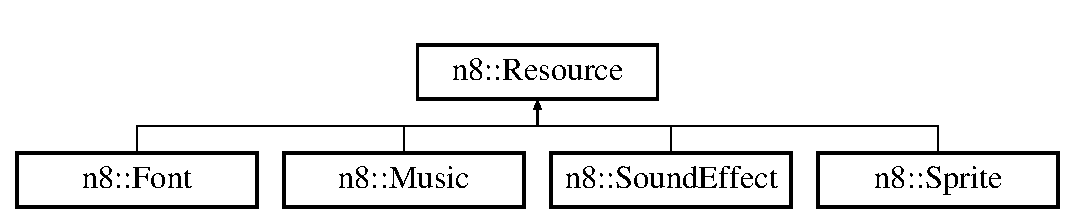
\includegraphics[height=2.000000cm]{classn8_1_1_resource}
\end{center}
\end{figure}
\subsection*{Public Member Functions}
\begin{DoxyCompactItemize}
\item 
\hyperlink{classn8_1_1_resource_ab779e9e31d429663b16d7d891494da7c}{Resource} (std\-::string p\-\_\-id)
\item 
virtual \hyperlink{classn8_1_1_resource_a238b22c42b4a9bc86509ed9c36bc4d2e}{$\sim$\-Resource} ()
\item 
std\-::string \hyperlink{classn8_1_1_resource_a18baa304ac93bd0b94b368ae64282f54}{Get\-Id} ()
\end{DoxyCompactItemize}
\subsection*{Private Attributes}
\begin{DoxyCompactItemize}
\item 
std\-::string \hyperlink{classn8_1_1_resource_a7a80eb975bb76b4e8c5b3b60de210f23}{m\-\_\-id}
\end{DoxyCompactItemize}


\subsection{Constructor \& Destructor Documentation}
\hypertarget{classn8_1_1_resource_ab779e9e31d429663b16d7d891494da7c}{\index{n8\-::\-Resource@{n8\-::\-Resource}!Resource@{Resource}}
\index{Resource@{Resource}!n8::Resource@{n8\-::\-Resource}}
\subsubsection[{Resource}]{\setlength{\rightskip}{0pt plus 5cm}n8\-::\-Resource\-::\-Resource (
\begin{DoxyParamCaption}
\item[{std\-::string}]{p\-\_\-id}
\end{DoxyParamCaption}
)\hspace{0.3cm}{\ttfamily [inline]}}}\label{classn8_1_1_resource_ab779e9e31d429663b16d7d891494da7c}
\hypertarget{classn8_1_1_resource_a238b22c42b4a9bc86509ed9c36bc4d2e}{\index{n8\-::\-Resource@{n8\-::\-Resource}!$\sim$\-Resource@{$\sim$\-Resource}}
\index{$\sim$\-Resource@{$\sim$\-Resource}!n8::Resource@{n8\-::\-Resource}}
\subsubsection[{$\sim$\-Resource}]{\setlength{\rightskip}{0pt plus 5cm}virtual n8\-::\-Resource\-::$\sim$\-Resource (
\begin{DoxyParamCaption}
{}
\end{DoxyParamCaption}
)\hspace{0.3cm}{\ttfamily [inline]}, {\ttfamily [virtual]}}}\label{classn8_1_1_resource_a238b22c42b4a9bc86509ed9c36bc4d2e}


\subsection{Member Function Documentation}
\hypertarget{classn8_1_1_resource_a18baa304ac93bd0b94b368ae64282f54}{\index{n8\-::\-Resource@{n8\-::\-Resource}!Get\-Id@{Get\-Id}}
\index{Get\-Id@{Get\-Id}!n8::Resource@{n8\-::\-Resource}}
\subsubsection[{Get\-Id}]{\setlength{\rightskip}{0pt plus 5cm}std\-::string n8\-::\-Resource\-::\-Get\-Id (
\begin{DoxyParamCaption}
{}
\end{DoxyParamCaption}
)\hspace{0.3cm}{\ttfamily [inline]}}}\label{classn8_1_1_resource_a18baa304ac93bd0b94b368ae64282f54}
\begin{DoxyReturn}{Returns}
The string id of the resource 
\end{DoxyReturn}


\subsection{Member Data Documentation}
\hypertarget{classn8_1_1_resource_a7a80eb975bb76b4e8c5b3b60de210f23}{\index{n8\-::\-Resource@{n8\-::\-Resource}!m\-\_\-id@{m\-\_\-id}}
\index{m\-\_\-id@{m\-\_\-id}!n8::Resource@{n8\-::\-Resource}}
\subsubsection[{m\-\_\-id}]{\setlength{\rightskip}{0pt plus 5cm}std\-::string n8\-::\-Resource\-::m\-\_\-id\hspace{0.3cm}{\ttfamily [private]}}}\label{classn8_1_1_resource_a7a80eb975bb76b4e8c5b3b60de210f23}


The documentation for this class was generated from the following file\-:\begin{DoxyCompactItemize}
\item 
Base/\hyperlink{_resource_8h}{Resource.\-h}\end{DoxyCompactItemize}

\hypertarget{classn8_1_1_resource_manager}{\section{n8\-:\-:Resource\-Manager Class Reference}
\label{classn8_1_1_resource_manager}\index{n8\-::\-Resource\-Manager@{n8\-::\-Resource\-Manager}}
}


Loads and stores game resources.  




{\ttfamily \#include $<$Resource\-Manager.\-h$>$}

Inheritance diagram for n8\-:\-:Resource\-Manager\-:\begin{figure}[H]
\begin{center}
\leavevmode
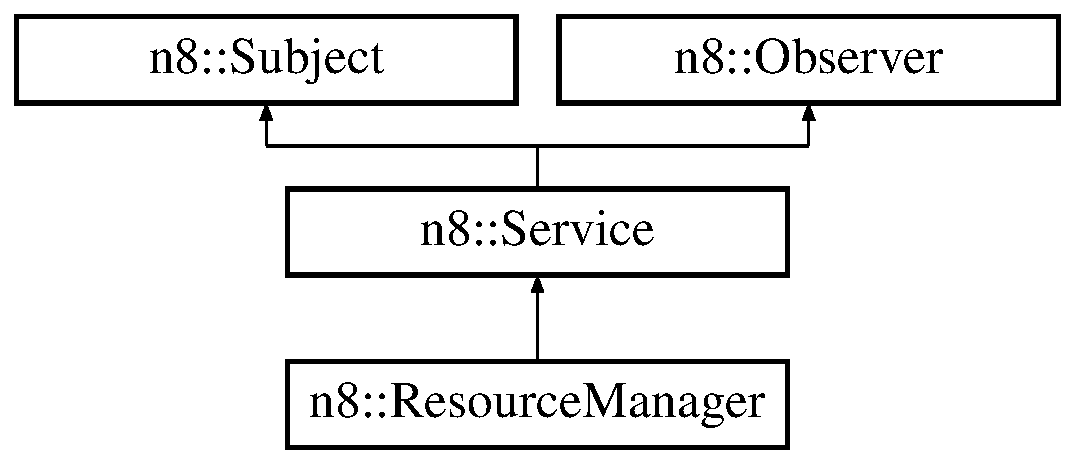
\includegraphics[height=3.000000cm]{classn8_1_1_resource_manager}
\end{center}
\end{figure}
\subsection*{Public Member Functions}
\begin{DoxyCompactItemize}
\item 
\hyperlink{classn8_1_1_resource_manager_a047ca08ea13d151e5c5162e4fae1c785}{Resource\-Manager} (S\-D\-L\-\_\-\-Surface $\ast$screen, std\-::string path)
\item 
\hyperlink{classn8_1_1_resource_manager_a06074da1d8fa5b1eb26e8a6996c6696e}{$\sim$\-Resource\-Manager} ()
\item 
\hyperlink{classn8_1_1_resource}{Resource} $\ast$ \hyperlink{classn8_1_1_resource_manager_a0d9c23c34a44338e53add156a88260bd}{Get\-Resource} (std\-::string)
\item 
void \hyperlink{classn8_1_1_resource_manager_ace97033b439ac0954cf2fc45a79081c9}{On\-Notify} (\hyperlink{classn8_1_1_event}{Event} $\ast$)
\end{DoxyCompactItemize}
\subsection*{Private Member Functions}
\begin{DoxyCompactItemize}
\item 
S\-D\-L\-\_\-\-Surface $\ast$ \hyperlink{classn8_1_1_resource_manager_acf5f0aafedcb3ed0c2a9b4e8518c8092}{Load\-Optimized\-Image} (std\-::string filename)
\item 
void \hyperlink{classn8_1_1_resource_manager_aa3424e9950ae39330cecba06286b6af1}{Load\-Resources} ()
\item 
void \hyperlink{classn8_1_1_resource_manager_ab8cb4600e3ee61439ddba958c2c1c3bf}{Load\-Sprite} (std\-::string, std\-::string)
\item 
void \hyperlink{classn8_1_1_resource_manager_a65cd9b6e010bdac87976e464c580b93a}{Load\-Texture} (std\-::string, std\-::string)
\item 
void \hyperlink{classn8_1_1_resource_manager_a21c0d9fbdf9413c4e5e9ac0e81461010}{Load\-Music} (std\-::string, std\-::string)
\item 
void \hyperlink{classn8_1_1_resource_manager_a38702603536a2f7c396cb0dcaab2df0d}{Load\-Sound\-Effect} (std\-::string, std\-::string)
\item 
void \hyperlink{classn8_1_1_resource_manager_ae80f49455160d64a2cf27099ba0d128f}{Load\-Font} (std\-::string, std\-::string, int)
\end{DoxyCompactItemize}
\subsection*{Private Attributes}
\begin{DoxyCompactItemize}
\item 
const std\-::string \hyperlink{classn8_1_1_resource_manager_aa8b18502df6a0b62127137c683d07f1c}{R\-E\-S\-O\-U\-R\-C\-E\-S\-\_\-\-T\-A\-G} = \char`\"{}Resources\char`\"{}
\item 
const std\-::string \hyperlink{classn8_1_1_resource_manager_a49db9fd91a84fdab02ddf86560677a72}{I\-M\-A\-G\-E\-\_\-\-R\-E\-S\-O\-U\-R\-C\-E\-S\-\_\-\-T\-A\-G} = \char`\"{}Image\-Resources\char`\"{}
\item 
const std\-::string \hyperlink{classn8_1_1_resource_manager_ad8a40ca4c1bfbd9ab2091a75ebf1d1b0}{S\-O\-U\-N\-D\-\_\-\-E\-F\-F\-E\-C\-T\-\_\-\-R\-E\-S\-O\-U\-R\-C\-E\-S\-\_\-\-T\-A\-G} = \char`\"{}Sound\-Effect\-Resources\char`\"{}
\item 
const std\-::string \hyperlink{classn8_1_1_resource_manager_a99df9f9f63f408c2173ded9cc234aee1}{M\-U\-S\-I\-C\-\_\-\-R\-E\-S\-O\-U\-R\-C\-E\-S\-\_\-\-T\-A\-G} = \char`\"{}Music\-Resources\char`\"{}
\item 
const std\-::string \hyperlink{classn8_1_1_resource_manager_aab02445c4198c8ffc987e19310b88264}{F\-O\-N\-T\-\_\-\-R\-E\-S\-O\-U\-R\-C\-E\-S\-\_\-\-T\-A\-G} = \char`\"{}Font\-Resources\char`\"{}
\item 
const std\-::string \hyperlink{classn8_1_1_resource_manager_a5070a7664d8876080169bb19d67c981e}{I\-M\-A\-G\-E\-\_\-\-T\-A\-G} = \char`\"{}Image\char`\"{}
\item 
const std\-::string \hyperlink{classn8_1_1_resource_manager_adddc8602373da08bf20c073087856f39}{S\-O\-U\-N\-D\-\_\-\-E\-F\-F\-E\-C\-T\-\_\-\-T\-A\-G} = \char`\"{}Sound\-Effect\char`\"{}
\item 
const std\-::string \hyperlink{classn8_1_1_resource_manager_a1ad23bd82f0c2b5ec4cda6b3f7c200f5}{M\-U\-S\-I\-C\-\_\-\-T\-A\-G} = \char`\"{}Music\char`\"{}
\item 
const std\-::string \hyperlink{classn8_1_1_resource_manager_a629c37bbc7cab402c22138873c447e76}{F\-O\-N\-T\-\_\-\-T\-A\-G} = \char`\"{}Font\char`\"{}
\item 
const std\-::string \hyperlink{classn8_1_1_resource_manager_ab2d2c6626b2c68384f1d400c17d1b38f}{S\-I\-Z\-E\-\_\-\-T\-A\-G} = \char`\"{}Size\char`\"{}
\item 
const std\-::string \hyperlink{classn8_1_1_resource_manager_a2893f0f975614d26af2b61e139d9acbe}{I\-D\-\_\-\-T\-A\-G} = \char`\"{}I\-D\char`\"{}
\item 
const std\-::string \hyperlink{classn8_1_1_resource_manager_ac7a0bd07466d2db724c71608a373c83e}{R\-E\-S\-O\-U\-R\-C\-E\-\_\-\-D\-I\-R\-E\-C\-T\-O\-R\-I\-E\-S\-\_\-\-P\-R\-E\-F\-I\-X} = \char`\"{}Resources\char`\"{}
\item 
const std\-::string \hyperlink{classn8_1_1_resource_manager_aa8fd98d5b987be54652a08f49e5ac7f7}{I\-M\-A\-G\-E\-S\-\_\-\-D\-I\-R\-E\-C\-T\-O\-R\-Y\-\_\-\-S\-U\-F\-F\-I\-X} = \char`\"{}Images\char`\"{}
\item 
const std\-::string \hyperlink{classn8_1_1_resource_manager_af0ddf0154273d7fa5fc31f63b5ce387c}{T\-E\-X\-T\-U\-R\-E\-S\-\_\-\-D\-I\-R\-E\-C\-T\-O\-R\-Y\-\_\-\-S\-U\-F\-F\-I\-X} = \char`\"{}Textures\char`\"{}
\item 
const std\-::string \hyperlink{classn8_1_1_resource_manager_a3bdb6e51b5a59ce6278d2ed13321edbb}{S\-O\-U\-N\-D\-\_\-\-E\-F\-F\-E\-C\-T\-\_\-\-D\-I\-R\-E\-C\-T\-O\-R\-Y\-\_\-\-S\-U\-F\-F\-I\-X} = \char`\"{}Sound\-Effect\char`\"{}
\item 
const std\-::string \hyperlink{classn8_1_1_resource_manager_af0d462dc1037e8377c297a02d53e761c}{M\-U\-S\-I\-C\-\_\-\-D\-I\-R\-E\-C\-T\-O\-R\-Y\-\_\-\-S\-U\-F\-F\-I\-X} = \char`\"{}Music\char`\"{}
\item 
const std\-::string \hyperlink{classn8_1_1_resource_manager_aa8b34428079b65912e1bcc4ffc04fbf1}{F\-O\-N\-T\-\_\-\-D\-I\-R\-E\-C\-T\-O\-R\-Y\-\_\-\-S\-U\-F\-F\-I\-X} = \char`\"{}Font\char`\"{}
\item 
std\-::string \hyperlink{classn8_1_1_resource_manager_a8b5220baaa8694b0229fea6ef8155d74}{m\-\_\-resources\-List\-Path}
\item 
std\-::map$<$ std\-::string, \hyperlink{classn8_1_1_resource}{Resource} $\ast$ $>$ \hyperlink{classn8_1_1_resource_manager_a1599b33c3fbe8b04045c2f39ea4ec80a}{m\-\_\-loaded\-Resources}
\item 
S\-D\-L\-\_\-\-Surface $\ast$ \hyperlink{classn8_1_1_resource_manager_a871c40637220ed8c82d230410aaf2aa2}{m\-\_\-screen\-Surface}
\end{DoxyCompactItemize}


\subsection{Detailed Description}
Loads and stores game resources. 

Loads resource information from an xml file. Attempts to load all specified data and store the neccessary resource objects using unique keys for lookup. The user can then request pointers to resource objects when needed. 

\subsection{Constructor \& Destructor Documentation}
\hypertarget{classn8_1_1_resource_manager_a047ca08ea13d151e5c5162e4fae1c785}{\index{n8\-::\-Resource\-Manager@{n8\-::\-Resource\-Manager}!Resource\-Manager@{Resource\-Manager}}
\index{Resource\-Manager@{Resource\-Manager}!n8::ResourceManager@{n8\-::\-Resource\-Manager}}
\subsubsection[{Resource\-Manager}]{\setlength{\rightskip}{0pt plus 5cm}n8\-::\-Resource\-Manager\-::\-Resource\-Manager (
\begin{DoxyParamCaption}
\item[{S\-D\-L\-\_\-\-Surface $\ast$}]{screen, }
\item[{std\-::string}]{path}
\end{DoxyParamCaption}
)}}\label{classn8_1_1_resource_manager_a047ca08ea13d151e5c5162e4fae1c785}
\hypertarget{classn8_1_1_resource_manager_a06074da1d8fa5b1eb26e8a6996c6696e}{\index{n8\-::\-Resource\-Manager@{n8\-::\-Resource\-Manager}!$\sim$\-Resource\-Manager@{$\sim$\-Resource\-Manager}}
\index{$\sim$\-Resource\-Manager@{$\sim$\-Resource\-Manager}!n8::ResourceManager@{n8\-::\-Resource\-Manager}}
\subsubsection[{$\sim$\-Resource\-Manager}]{\setlength{\rightskip}{0pt plus 5cm}n8\-::\-Resource\-Manager\-::$\sim$\-Resource\-Manager (
\begin{DoxyParamCaption}
{}
\end{DoxyParamCaption}
)}}\label{classn8_1_1_resource_manager_a06074da1d8fa5b1eb26e8a6996c6696e}
Destructor Deletes all loaded resources 

\subsection{Member Function Documentation}
\hypertarget{classn8_1_1_resource_manager_a0d9c23c34a44338e53add156a88260bd}{\index{n8\-::\-Resource\-Manager@{n8\-::\-Resource\-Manager}!Get\-Resource@{Get\-Resource}}
\index{Get\-Resource@{Get\-Resource}!n8::ResourceManager@{n8\-::\-Resource\-Manager}}
\subsubsection[{Get\-Resource}]{\setlength{\rightskip}{0pt plus 5cm}{\bf n8\-::\-Resource} $\ast$ n8\-::\-Resource\-Manager\-::\-Get\-Resource (
\begin{DoxyParamCaption}
\item[{std\-::string}]{p\-\_\-resource\-I\-D}
\end{DoxyParamCaption}
)}}\label{classn8_1_1_resource_manager_a0d9c23c34a44338e53add156a88260bd}
Get\-Resource Used to get resource object pointers from the resource manager


\begin{DoxyParams}{Parameters}
{\em p\-\_\-resource\-I\-D} & The identifier for the desired resource. Used as the key for looking up the resource in the resource map\\
\hline
\end{DoxyParams}
\begin{DoxyReturn}{Returns}
Pointer to a resource object matching the passed key, N\-U\-L\-L otherwise 
\end{DoxyReturn}
\hypertarget{classn8_1_1_resource_manager_ae80f49455160d64a2cf27099ba0d128f}{\index{n8\-::\-Resource\-Manager@{n8\-::\-Resource\-Manager}!Load\-Font@{Load\-Font}}
\index{Load\-Font@{Load\-Font}!n8::ResourceManager@{n8\-::\-Resource\-Manager}}
\subsubsection[{Load\-Font}]{\setlength{\rightskip}{0pt plus 5cm}void n8\-::\-Resource\-Manager\-::\-Load\-Font (
\begin{DoxyParamCaption}
\item[{std\-::string}]{p\-\_\-filename, }
\item[{std\-::string}]{p\-\_\-id, }
\item[{int}]{p\-\_\-size}
\end{DoxyParamCaption}
)\hspace{0.3cm}{\ttfamily [private]}}}\label{classn8_1_1_resource_manager_ae80f49455160d64a2cf27099ba0d128f}
Load\-Font Loads font resources specified by Resources.\-xml


\begin{DoxyParams}{Parameters}
{\em p\-\_\-filename} & Filename of font to load \\
\hline
{\em p\-\_\-id} & The identifier for the font object. Acts as the key for the object in the resource map \\
\hline
{\em p\-\_\-size} & The font size of the desired font object \\
\hline
\end{DoxyParams}
\hypertarget{classn8_1_1_resource_manager_a21c0d9fbdf9413c4e5e9ac0e81461010}{\index{n8\-::\-Resource\-Manager@{n8\-::\-Resource\-Manager}!Load\-Music@{Load\-Music}}
\index{Load\-Music@{Load\-Music}!n8::ResourceManager@{n8\-::\-Resource\-Manager}}
\subsubsection[{Load\-Music}]{\setlength{\rightskip}{0pt plus 5cm}void n8\-::\-Resource\-Manager\-::\-Load\-Music (
\begin{DoxyParamCaption}
\item[{std\-::string}]{p\-\_\-filename, }
\item[{std\-::string}]{p\-\_\-id}
\end{DoxyParamCaption}
)\hspace{0.3cm}{\ttfamily [private]}}}\label{classn8_1_1_resource_manager_a21c0d9fbdf9413c4e5e9ac0e81461010}
Loads music resources


\begin{DoxyParams}{Parameters}
{\em p\-\_\-filename} & Name of the resource file to load into a \hyperlink{classn8_1_1_music}{Music} object \\
\hline
\end{DoxyParams}
\hypertarget{classn8_1_1_resource_manager_acf5f0aafedcb3ed0c2a9b4e8518c8092}{\index{n8\-::\-Resource\-Manager@{n8\-::\-Resource\-Manager}!Load\-Optimized\-Image@{Load\-Optimized\-Image}}
\index{Load\-Optimized\-Image@{Load\-Optimized\-Image}!n8::ResourceManager@{n8\-::\-Resource\-Manager}}
\subsubsection[{Load\-Optimized\-Image}]{\setlength{\rightskip}{0pt plus 5cm}S\-D\-L\-\_\-\-Surface $\ast$ n8\-::\-Resource\-Manager\-::\-Load\-Optimized\-Image (
\begin{DoxyParamCaption}
\item[{std\-::string}]{filename}
\end{DoxyParamCaption}
)\hspace{0.3cm}{\ttfamily [private]}}}\label{classn8_1_1_resource_manager_acf5f0aafedcb3ed0c2a9b4e8518c8092}
Loads an image from a specified filepath, then creates an optimzed copy of the image


\begin{DoxyParams}{Parameters}
{\em filename} & the filename of the image to load and optimize \\
\hline
\end{DoxyParams}
\begin{DoxyReturn}{Returns}
a pointer to the optimized copy of the image 
\end{DoxyReturn}
\hypertarget{classn8_1_1_resource_manager_aa3424e9950ae39330cecba06286b6af1}{\index{n8\-::\-Resource\-Manager@{n8\-::\-Resource\-Manager}!Load\-Resources@{Load\-Resources}}
\index{Load\-Resources@{Load\-Resources}!n8::ResourceManager@{n8\-::\-Resource\-Manager}}
\subsubsection[{Load\-Resources}]{\setlength{\rightskip}{0pt plus 5cm}void n8\-::\-Resource\-Manager\-::\-Load\-Resources (
\begin{DoxyParamCaption}
{}
\end{DoxyParamCaption}
)\hspace{0.3cm}{\ttfamily [private]}}}\label{classn8_1_1_resource_manager_aa3424e9950ae39330cecba06286b6af1}
\hypertarget{classn8_1_1_resource_manager_a38702603536a2f7c396cb0dcaab2df0d}{\index{n8\-::\-Resource\-Manager@{n8\-::\-Resource\-Manager}!Load\-Sound\-Effect@{Load\-Sound\-Effect}}
\index{Load\-Sound\-Effect@{Load\-Sound\-Effect}!n8::ResourceManager@{n8\-::\-Resource\-Manager}}
\subsubsection[{Load\-Sound\-Effect}]{\setlength{\rightskip}{0pt plus 5cm}void n8\-::\-Resource\-Manager\-::\-Load\-Sound\-Effect (
\begin{DoxyParamCaption}
\item[{std\-::string}]{p\-\_\-filename, }
\item[{std\-::string}]{p\-\_\-id}
\end{DoxyParamCaption}
)\hspace{0.3cm}{\ttfamily [private]}}}\label{classn8_1_1_resource_manager_a38702603536a2f7c396cb0dcaab2df0d}
Loads sound effect resources


\begin{DoxyParams}{Parameters}
{\em p\-\_\-filename} & Name of the resource file to load into a \hyperlink{classn8_1_1_sound_effect}{Sound\-Effect} object \\
\hline
{\em p\-\_\-id} & The identifier for the \hyperlink{classn8_1_1_sound_effect}{Sound\-Effect} object. Acts as the key for the object in the resource map \\
\hline
\end{DoxyParams}
\hypertarget{classn8_1_1_resource_manager_ab8cb4600e3ee61439ddba958c2c1c3bf}{\index{n8\-::\-Resource\-Manager@{n8\-::\-Resource\-Manager}!Load\-Sprite@{Load\-Sprite}}
\index{Load\-Sprite@{Load\-Sprite}!n8::ResourceManager@{n8\-::\-Resource\-Manager}}
\subsubsection[{Load\-Sprite}]{\setlength{\rightskip}{0pt plus 5cm}void n8\-::\-Resource\-Manager\-::\-Load\-Sprite (
\begin{DoxyParamCaption}
\item[{std\-::string}]{p\-\_\-filename, }
\item[{std\-::string}]{p\-\_\-id}
\end{DoxyParamCaption}
)\hspace{0.3cm}{\ttfamily [private]}}}\label{classn8_1_1_resource_manager_ab8cb4600e3ee61439ddba958c2c1c3bf}
Loads \hyperlink{classn8_1_1_sprite}{Sprite} resources. Currently not implemented. \hypertarget{classn8_1_1_resource_manager_a65cd9b6e010bdac87976e464c580b93a}{\index{n8\-::\-Resource\-Manager@{n8\-::\-Resource\-Manager}!Load\-Texture@{Load\-Texture}}
\index{Load\-Texture@{Load\-Texture}!n8::ResourceManager@{n8\-::\-Resource\-Manager}}
\subsubsection[{Load\-Texture}]{\setlength{\rightskip}{0pt plus 5cm}void n8\-::\-Resource\-Manager\-::\-Load\-Texture (
\begin{DoxyParamCaption}
\item[{std\-::string}]{p\-\_\-filename, }
\item[{std\-::string}]{p\-\_\-id}
\end{DoxyParamCaption}
)\hspace{0.3cm}{\ttfamily [private]}}}\label{classn8_1_1_resource_manager_a65cd9b6e010bdac87976e464c580b93a}
Loads Texture resources. Currently not implemented \hypertarget{classn8_1_1_resource_manager_ace97033b439ac0954cf2fc45a79081c9}{\index{n8\-::\-Resource\-Manager@{n8\-::\-Resource\-Manager}!On\-Notify@{On\-Notify}}
\index{On\-Notify@{On\-Notify}!n8::ResourceManager@{n8\-::\-Resource\-Manager}}
\subsubsection[{On\-Notify}]{\setlength{\rightskip}{0pt plus 5cm}void n8\-::\-Resource\-Manager\-::\-On\-Notify (
\begin{DoxyParamCaption}
\item[{{\bf n8\-::\-Event} $\ast$}]{event}
\end{DoxyParamCaption}
)\hspace{0.3cm}{\ttfamily [virtual]}}}\label{classn8_1_1_resource_manager_ace97033b439ac0954cf2fc45a79081c9}


Implements \hyperlink{classn8_1_1_service_a756a170eba7e5c34a1c12008e22d3ca7}{n8\-::\-Service}.



\subsection{Member Data Documentation}
\hypertarget{classn8_1_1_resource_manager_aa8b34428079b65912e1bcc4ffc04fbf1}{\index{n8\-::\-Resource\-Manager@{n8\-::\-Resource\-Manager}!F\-O\-N\-T\-\_\-\-D\-I\-R\-E\-C\-T\-O\-R\-Y\-\_\-\-S\-U\-F\-F\-I\-X@{F\-O\-N\-T\-\_\-\-D\-I\-R\-E\-C\-T\-O\-R\-Y\-\_\-\-S\-U\-F\-F\-I\-X}}
\index{F\-O\-N\-T\-\_\-\-D\-I\-R\-E\-C\-T\-O\-R\-Y\-\_\-\-S\-U\-F\-F\-I\-X@{F\-O\-N\-T\-\_\-\-D\-I\-R\-E\-C\-T\-O\-R\-Y\-\_\-\-S\-U\-F\-F\-I\-X}!n8::ResourceManager@{n8\-::\-Resource\-Manager}}
\subsubsection[{F\-O\-N\-T\-\_\-\-D\-I\-R\-E\-C\-T\-O\-R\-Y\-\_\-\-S\-U\-F\-F\-I\-X}]{\setlength{\rightskip}{0pt plus 5cm}const std\-::string n8\-::\-Resource\-Manager\-::\-F\-O\-N\-T\-\_\-\-D\-I\-R\-E\-C\-T\-O\-R\-Y\-\_\-\-S\-U\-F\-F\-I\-X = \char`\"{}Font\char`\"{}\hspace{0.3cm}{\ttfamily [private]}}}\label{classn8_1_1_resource_manager_aa8b34428079b65912e1bcc4ffc04fbf1}
\hypertarget{classn8_1_1_resource_manager_aab02445c4198c8ffc987e19310b88264}{\index{n8\-::\-Resource\-Manager@{n8\-::\-Resource\-Manager}!F\-O\-N\-T\-\_\-\-R\-E\-S\-O\-U\-R\-C\-E\-S\-\_\-\-T\-A\-G@{F\-O\-N\-T\-\_\-\-R\-E\-S\-O\-U\-R\-C\-E\-S\-\_\-\-T\-A\-G}}
\index{F\-O\-N\-T\-\_\-\-R\-E\-S\-O\-U\-R\-C\-E\-S\-\_\-\-T\-A\-G@{F\-O\-N\-T\-\_\-\-R\-E\-S\-O\-U\-R\-C\-E\-S\-\_\-\-T\-A\-G}!n8::ResourceManager@{n8\-::\-Resource\-Manager}}
\subsubsection[{F\-O\-N\-T\-\_\-\-R\-E\-S\-O\-U\-R\-C\-E\-S\-\_\-\-T\-A\-G}]{\setlength{\rightskip}{0pt plus 5cm}const std\-::string n8\-::\-Resource\-Manager\-::\-F\-O\-N\-T\-\_\-\-R\-E\-S\-O\-U\-R\-C\-E\-S\-\_\-\-T\-A\-G = \char`\"{}Font\-Resources\char`\"{}\hspace{0.3cm}{\ttfamily [private]}}}\label{classn8_1_1_resource_manager_aab02445c4198c8ffc987e19310b88264}
\hypertarget{classn8_1_1_resource_manager_a629c37bbc7cab402c22138873c447e76}{\index{n8\-::\-Resource\-Manager@{n8\-::\-Resource\-Manager}!F\-O\-N\-T\-\_\-\-T\-A\-G@{F\-O\-N\-T\-\_\-\-T\-A\-G}}
\index{F\-O\-N\-T\-\_\-\-T\-A\-G@{F\-O\-N\-T\-\_\-\-T\-A\-G}!n8::ResourceManager@{n8\-::\-Resource\-Manager}}
\subsubsection[{F\-O\-N\-T\-\_\-\-T\-A\-G}]{\setlength{\rightskip}{0pt plus 5cm}const std\-::string n8\-::\-Resource\-Manager\-::\-F\-O\-N\-T\-\_\-\-T\-A\-G = \char`\"{}Font\char`\"{}\hspace{0.3cm}{\ttfamily [private]}}}\label{classn8_1_1_resource_manager_a629c37bbc7cab402c22138873c447e76}
\hypertarget{classn8_1_1_resource_manager_a2893f0f975614d26af2b61e139d9acbe}{\index{n8\-::\-Resource\-Manager@{n8\-::\-Resource\-Manager}!I\-D\-\_\-\-T\-A\-G@{I\-D\-\_\-\-T\-A\-G}}
\index{I\-D\-\_\-\-T\-A\-G@{I\-D\-\_\-\-T\-A\-G}!n8::ResourceManager@{n8\-::\-Resource\-Manager}}
\subsubsection[{I\-D\-\_\-\-T\-A\-G}]{\setlength{\rightskip}{0pt plus 5cm}const std\-::string n8\-::\-Resource\-Manager\-::\-I\-D\-\_\-\-T\-A\-G = \char`\"{}I\-D\char`\"{}\hspace{0.3cm}{\ttfamily [private]}}}\label{classn8_1_1_resource_manager_a2893f0f975614d26af2b61e139d9acbe}
\hypertarget{classn8_1_1_resource_manager_a49db9fd91a84fdab02ddf86560677a72}{\index{n8\-::\-Resource\-Manager@{n8\-::\-Resource\-Manager}!I\-M\-A\-G\-E\-\_\-\-R\-E\-S\-O\-U\-R\-C\-E\-S\-\_\-\-T\-A\-G@{I\-M\-A\-G\-E\-\_\-\-R\-E\-S\-O\-U\-R\-C\-E\-S\-\_\-\-T\-A\-G}}
\index{I\-M\-A\-G\-E\-\_\-\-R\-E\-S\-O\-U\-R\-C\-E\-S\-\_\-\-T\-A\-G@{I\-M\-A\-G\-E\-\_\-\-R\-E\-S\-O\-U\-R\-C\-E\-S\-\_\-\-T\-A\-G}!n8::ResourceManager@{n8\-::\-Resource\-Manager}}
\subsubsection[{I\-M\-A\-G\-E\-\_\-\-R\-E\-S\-O\-U\-R\-C\-E\-S\-\_\-\-T\-A\-G}]{\setlength{\rightskip}{0pt plus 5cm}const std\-::string n8\-::\-Resource\-Manager\-::\-I\-M\-A\-G\-E\-\_\-\-R\-E\-S\-O\-U\-R\-C\-E\-S\-\_\-\-T\-A\-G = \char`\"{}Image\-Resources\char`\"{}\hspace{0.3cm}{\ttfamily [private]}}}\label{classn8_1_1_resource_manager_a49db9fd91a84fdab02ddf86560677a72}
\hypertarget{classn8_1_1_resource_manager_a5070a7664d8876080169bb19d67c981e}{\index{n8\-::\-Resource\-Manager@{n8\-::\-Resource\-Manager}!I\-M\-A\-G\-E\-\_\-\-T\-A\-G@{I\-M\-A\-G\-E\-\_\-\-T\-A\-G}}
\index{I\-M\-A\-G\-E\-\_\-\-T\-A\-G@{I\-M\-A\-G\-E\-\_\-\-T\-A\-G}!n8::ResourceManager@{n8\-::\-Resource\-Manager}}
\subsubsection[{I\-M\-A\-G\-E\-\_\-\-T\-A\-G}]{\setlength{\rightskip}{0pt plus 5cm}const std\-::string n8\-::\-Resource\-Manager\-::\-I\-M\-A\-G\-E\-\_\-\-T\-A\-G = \char`\"{}Image\char`\"{}\hspace{0.3cm}{\ttfamily [private]}}}\label{classn8_1_1_resource_manager_a5070a7664d8876080169bb19d67c981e}
\hypertarget{classn8_1_1_resource_manager_aa8fd98d5b987be54652a08f49e5ac7f7}{\index{n8\-::\-Resource\-Manager@{n8\-::\-Resource\-Manager}!I\-M\-A\-G\-E\-S\-\_\-\-D\-I\-R\-E\-C\-T\-O\-R\-Y\-\_\-\-S\-U\-F\-F\-I\-X@{I\-M\-A\-G\-E\-S\-\_\-\-D\-I\-R\-E\-C\-T\-O\-R\-Y\-\_\-\-S\-U\-F\-F\-I\-X}}
\index{I\-M\-A\-G\-E\-S\-\_\-\-D\-I\-R\-E\-C\-T\-O\-R\-Y\-\_\-\-S\-U\-F\-F\-I\-X@{I\-M\-A\-G\-E\-S\-\_\-\-D\-I\-R\-E\-C\-T\-O\-R\-Y\-\_\-\-S\-U\-F\-F\-I\-X}!n8::ResourceManager@{n8\-::\-Resource\-Manager}}
\subsubsection[{I\-M\-A\-G\-E\-S\-\_\-\-D\-I\-R\-E\-C\-T\-O\-R\-Y\-\_\-\-S\-U\-F\-F\-I\-X}]{\setlength{\rightskip}{0pt plus 5cm}const std\-::string n8\-::\-Resource\-Manager\-::\-I\-M\-A\-G\-E\-S\-\_\-\-D\-I\-R\-E\-C\-T\-O\-R\-Y\-\_\-\-S\-U\-F\-F\-I\-X = \char`\"{}Images\char`\"{}\hspace{0.3cm}{\ttfamily [private]}}}\label{classn8_1_1_resource_manager_aa8fd98d5b987be54652a08f49e5ac7f7}
\hypertarget{classn8_1_1_resource_manager_a1599b33c3fbe8b04045c2f39ea4ec80a}{\index{n8\-::\-Resource\-Manager@{n8\-::\-Resource\-Manager}!m\-\_\-loaded\-Resources@{m\-\_\-loaded\-Resources}}
\index{m\-\_\-loaded\-Resources@{m\-\_\-loaded\-Resources}!n8::ResourceManager@{n8\-::\-Resource\-Manager}}
\subsubsection[{m\-\_\-loaded\-Resources}]{\setlength{\rightskip}{0pt plus 5cm}std\-::map$<$std\-::string,{\bf Resource}$\ast$$>$ n8\-::\-Resource\-Manager\-::m\-\_\-loaded\-Resources\hspace{0.3cm}{\ttfamily [private]}}}\label{classn8_1_1_resource_manager_a1599b33c3fbe8b04045c2f39ea4ec80a}
Stores all images loaded by the system \hypertarget{classn8_1_1_resource_manager_a8b5220baaa8694b0229fea6ef8155d74}{\index{n8\-::\-Resource\-Manager@{n8\-::\-Resource\-Manager}!m\-\_\-resources\-List\-Path@{m\-\_\-resources\-List\-Path}}
\index{m\-\_\-resources\-List\-Path@{m\-\_\-resources\-List\-Path}!n8::ResourceManager@{n8\-::\-Resource\-Manager}}
\subsubsection[{m\-\_\-resources\-List\-Path}]{\setlength{\rightskip}{0pt plus 5cm}std\-::string n8\-::\-Resource\-Manager\-::m\-\_\-resources\-List\-Path\hspace{0.3cm}{\ttfamily [private]}}}\label{classn8_1_1_resource_manager_a8b5220baaa8694b0229fea6ef8155d74}
Filepath to the resource list \hypertarget{classn8_1_1_resource_manager_a871c40637220ed8c82d230410aaf2aa2}{\index{n8\-::\-Resource\-Manager@{n8\-::\-Resource\-Manager}!m\-\_\-screen\-Surface@{m\-\_\-screen\-Surface}}
\index{m\-\_\-screen\-Surface@{m\-\_\-screen\-Surface}!n8::ResourceManager@{n8\-::\-Resource\-Manager}}
\subsubsection[{m\-\_\-screen\-Surface}]{\setlength{\rightskip}{0pt plus 5cm}S\-D\-L\-\_\-\-Surface$\ast$ n8\-::\-Resource\-Manager\-::m\-\_\-screen\-Surface\hspace{0.3cm}{\ttfamily [private]}}}\label{classn8_1_1_resource_manager_a871c40637220ed8c82d230410aaf2aa2}
Stores pointer to the game's screen surface. Used to load optimized versions of images \hypertarget{classn8_1_1_resource_manager_af0d462dc1037e8377c297a02d53e761c}{\index{n8\-::\-Resource\-Manager@{n8\-::\-Resource\-Manager}!M\-U\-S\-I\-C\-\_\-\-D\-I\-R\-E\-C\-T\-O\-R\-Y\-\_\-\-S\-U\-F\-F\-I\-X@{M\-U\-S\-I\-C\-\_\-\-D\-I\-R\-E\-C\-T\-O\-R\-Y\-\_\-\-S\-U\-F\-F\-I\-X}}
\index{M\-U\-S\-I\-C\-\_\-\-D\-I\-R\-E\-C\-T\-O\-R\-Y\-\_\-\-S\-U\-F\-F\-I\-X@{M\-U\-S\-I\-C\-\_\-\-D\-I\-R\-E\-C\-T\-O\-R\-Y\-\_\-\-S\-U\-F\-F\-I\-X}!n8::ResourceManager@{n8\-::\-Resource\-Manager}}
\subsubsection[{M\-U\-S\-I\-C\-\_\-\-D\-I\-R\-E\-C\-T\-O\-R\-Y\-\_\-\-S\-U\-F\-F\-I\-X}]{\setlength{\rightskip}{0pt plus 5cm}const std\-::string n8\-::\-Resource\-Manager\-::\-M\-U\-S\-I\-C\-\_\-\-D\-I\-R\-E\-C\-T\-O\-R\-Y\-\_\-\-S\-U\-F\-F\-I\-X = \char`\"{}Music\char`\"{}\hspace{0.3cm}{\ttfamily [private]}}}\label{classn8_1_1_resource_manager_af0d462dc1037e8377c297a02d53e761c}
\hypertarget{classn8_1_1_resource_manager_a99df9f9f63f408c2173ded9cc234aee1}{\index{n8\-::\-Resource\-Manager@{n8\-::\-Resource\-Manager}!M\-U\-S\-I\-C\-\_\-\-R\-E\-S\-O\-U\-R\-C\-E\-S\-\_\-\-T\-A\-G@{M\-U\-S\-I\-C\-\_\-\-R\-E\-S\-O\-U\-R\-C\-E\-S\-\_\-\-T\-A\-G}}
\index{M\-U\-S\-I\-C\-\_\-\-R\-E\-S\-O\-U\-R\-C\-E\-S\-\_\-\-T\-A\-G@{M\-U\-S\-I\-C\-\_\-\-R\-E\-S\-O\-U\-R\-C\-E\-S\-\_\-\-T\-A\-G}!n8::ResourceManager@{n8\-::\-Resource\-Manager}}
\subsubsection[{M\-U\-S\-I\-C\-\_\-\-R\-E\-S\-O\-U\-R\-C\-E\-S\-\_\-\-T\-A\-G}]{\setlength{\rightskip}{0pt plus 5cm}const std\-::string n8\-::\-Resource\-Manager\-::\-M\-U\-S\-I\-C\-\_\-\-R\-E\-S\-O\-U\-R\-C\-E\-S\-\_\-\-T\-A\-G = \char`\"{}Music\-Resources\char`\"{}\hspace{0.3cm}{\ttfamily [private]}}}\label{classn8_1_1_resource_manager_a99df9f9f63f408c2173ded9cc234aee1}
\hypertarget{classn8_1_1_resource_manager_a1ad23bd82f0c2b5ec4cda6b3f7c200f5}{\index{n8\-::\-Resource\-Manager@{n8\-::\-Resource\-Manager}!M\-U\-S\-I\-C\-\_\-\-T\-A\-G@{M\-U\-S\-I\-C\-\_\-\-T\-A\-G}}
\index{M\-U\-S\-I\-C\-\_\-\-T\-A\-G@{M\-U\-S\-I\-C\-\_\-\-T\-A\-G}!n8::ResourceManager@{n8\-::\-Resource\-Manager}}
\subsubsection[{M\-U\-S\-I\-C\-\_\-\-T\-A\-G}]{\setlength{\rightskip}{0pt plus 5cm}const std\-::string n8\-::\-Resource\-Manager\-::\-M\-U\-S\-I\-C\-\_\-\-T\-A\-G = \char`\"{}Music\char`\"{}\hspace{0.3cm}{\ttfamily [private]}}}\label{classn8_1_1_resource_manager_a1ad23bd82f0c2b5ec4cda6b3f7c200f5}
\hypertarget{classn8_1_1_resource_manager_ac7a0bd07466d2db724c71608a373c83e}{\index{n8\-::\-Resource\-Manager@{n8\-::\-Resource\-Manager}!R\-E\-S\-O\-U\-R\-C\-E\-\_\-\-D\-I\-R\-E\-C\-T\-O\-R\-I\-E\-S\-\_\-\-P\-R\-E\-F\-I\-X@{R\-E\-S\-O\-U\-R\-C\-E\-\_\-\-D\-I\-R\-E\-C\-T\-O\-R\-I\-E\-S\-\_\-\-P\-R\-E\-F\-I\-X}}
\index{R\-E\-S\-O\-U\-R\-C\-E\-\_\-\-D\-I\-R\-E\-C\-T\-O\-R\-I\-E\-S\-\_\-\-P\-R\-E\-F\-I\-X@{R\-E\-S\-O\-U\-R\-C\-E\-\_\-\-D\-I\-R\-E\-C\-T\-O\-R\-I\-E\-S\-\_\-\-P\-R\-E\-F\-I\-X}!n8::ResourceManager@{n8\-::\-Resource\-Manager}}
\subsubsection[{R\-E\-S\-O\-U\-R\-C\-E\-\_\-\-D\-I\-R\-E\-C\-T\-O\-R\-I\-E\-S\-\_\-\-P\-R\-E\-F\-I\-X}]{\setlength{\rightskip}{0pt plus 5cm}const std\-::string n8\-::\-Resource\-Manager\-::\-R\-E\-S\-O\-U\-R\-C\-E\-\_\-\-D\-I\-R\-E\-C\-T\-O\-R\-I\-E\-S\-\_\-\-P\-R\-E\-F\-I\-X = \char`\"{}Resources\char`\"{}\hspace{0.3cm}{\ttfamily [private]}}}\label{classn8_1_1_resource_manager_ac7a0bd07466d2db724c71608a373c83e}
\hypertarget{classn8_1_1_resource_manager_aa8b18502df6a0b62127137c683d07f1c}{\index{n8\-::\-Resource\-Manager@{n8\-::\-Resource\-Manager}!R\-E\-S\-O\-U\-R\-C\-E\-S\-\_\-\-T\-A\-G@{R\-E\-S\-O\-U\-R\-C\-E\-S\-\_\-\-T\-A\-G}}
\index{R\-E\-S\-O\-U\-R\-C\-E\-S\-\_\-\-T\-A\-G@{R\-E\-S\-O\-U\-R\-C\-E\-S\-\_\-\-T\-A\-G}!n8::ResourceManager@{n8\-::\-Resource\-Manager}}
\subsubsection[{R\-E\-S\-O\-U\-R\-C\-E\-S\-\_\-\-T\-A\-G}]{\setlength{\rightskip}{0pt plus 5cm}const std\-::string n8\-::\-Resource\-Manager\-::\-R\-E\-S\-O\-U\-R\-C\-E\-S\-\_\-\-T\-A\-G = \char`\"{}Resources\char`\"{}\hspace{0.3cm}{\ttfamily [private]}}}\label{classn8_1_1_resource_manager_aa8b18502df6a0b62127137c683d07f1c}
\hypertarget{classn8_1_1_resource_manager_ab2d2c6626b2c68384f1d400c17d1b38f}{\index{n8\-::\-Resource\-Manager@{n8\-::\-Resource\-Manager}!S\-I\-Z\-E\-\_\-\-T\-A\-G@{S\-I\-Z\-E\-\_\-\-T\-A\-G}}
\index{S\-I\-Z\-E\-\_\-\-T\-A\-G@{S\-I\-Z\-E\-\_\-\-T\-A\-G}!n8::ResourceManager@{n8\-::\-Resource\-Manager}}
\subsubsection[{S\-I\-Z\-E\-\_\-\-T\-A\-G}]{\setlength{\rightskip}{0pt plus 5cm}const std\-::string n8\-::\-Resource\-Manager\-::\-S\-I\-Z\-E\-\_\-\-T\-A\-G = \char`\"{}Size\char`\"{}\hspace{0.3cm}{\ttfamily [private]}}}\label{classn8_1_1_resource_manager_ab2d2c6626b2c68384f1d400c17d1b38f}
\hypertarget{classn8_1_1_resource_manager_a3bdb6e51b5a59ce6278d2ed13321edbb}{\index{n8\-::\-Resource\-Manager@{n8\-::\-Resource\-Manager}!S\-O\-U\-N\-D\-\_\-\-E\-F\-F\-E\-C\-T\-\_\-\-D\-I\-R\-E\-C\-T\-O\-R\-Y\-\_\-\-S\-U\-F\-F\-I\-X@{S\-O\-U\-N\-D\-\_\-\-E\-F\-F\-E\-C\-T\-\_\-\-D\-I\-R\-E\-C\-T\-O\-R\-Y\-\_\-\-S\-U\-F\-F\-I\-X}}
\index{S\-O\-U\-N\-D\-\_\-\-E\-F\-F\-E\-C\-T\-\_\-\-D\-I\-R\-E\-C\-T\-O\-R\-Y\-\_\-\-S\-U\-F\-F\-I\-X@{S\-O\-U\-N\-D\-\_\-\-E\-F\-F\-E\-C\-T\-\_\-\-D\-I\-R\-E\-C\-T\-O\-R\-Y\-\_\-\-S\-U\-F\-F\-I\-X}!n8::ResourceManager@{n8\-::\-Resource\-Manager}}
\subsubsection[{S\-O\-U\-N\-D\-\_\-\-E\-F\-F\-E\-C\-T\-\_\-\-D\-I\-R\-E\-C\-T\-O\-R\-Y\-\_\-\-S\-U\-F\-F\-I\-X}]{\setlength{\rightskip}{0pt plus 5cm}const std\-::string n8\-::\-Resource\-Manager\-::\-S\-O\-U\-N\-D\-\_\-\-E\-F\-F\-E\-C\-T\-\_\-\-D\-I\-R\-E\-C\-T\-O\-R\-Y\-\_\-\-S\-U\-F\-F\-I\-X = \char`\"{}Sound\-Effect\char`\"{}\hspace{0.3cm}{\ttfamily [private]}}}\label{classn8_1_1_resource_manager_a3bdb6e51b5a59ce6278d2ed13321edbb}
\hypertarget{classn8_1_1_resource_manager_ad8a40ca4c1bfbd9ab2091a75ebf1d1b0}{\index{n8\-::\-Resource\-Manager@{n8\-::\-Resource\-Manager}!S\-O\-U\-N\-D\-\_\-\-E\-F\-F\-E\-C\-T\-\_\-\-R\-E\-S\-O\-U\-R\-C\-E\-S\-\_\-\-T\-A\-G@{S\-O\-U\-N\-D\-\_\-\-E\-F\-F\-E\-C\-T\-\_\-\-R\-E\-S\-O\-U\-R\-C\-E\-S\-\_\-\-T\-A\-G}}
\index{S\-O\-U\-N\-D\-\_\-\-E\-F\-F\-E\-C\-T\-\_\-\-R\-E\-S\-O\-U\-R\-C\-E\-S\-\_\-\-T\-A\-G@{S\-O\-U\-N\-D\-\_\-\-E\-F\-F\-E\-C\-T\-\_\-\-R\-E\-S\-O\-U\-R\-C\-E\-S\-\_\-\-T\-A\-G}!n8::ResourceManager@{n8\-::\-Resource\-Manager}}
\subsubsection[{S\-O\-U\-N\-D\-\_\-\-E\-F\-F\-E\-C\-T\-\_\-\-R\-E\-S\-O\-U\-R\-C\-E\-S\-\_\-\-T\-A\-G}]{\setlength{\rightskip}{0pt plus 5cm}const std\-::string n8\-::\-Resource\-Manager\-::\-S\-O\-U\-N\-D\-\_\-\-E\-F\-F\-E\-C\-T\-\_\-\-R\-E\-S\-O\-U\-R\-C\-E\-S\-\_\-\-T\-A\-G = \char`\"{}Sound\-Effect\-Resources\char`\"{}\hspace{0.3cm}{\ttfamily [private]}}}\label{classn8_1_1_resource_manager_ad8a40ca4c1bfbd9ab2091a75ebf1d1b0}
\hypertarget{classn8_1_1_resource_manager_adddc8602373da08bf20c073087856f39}{\index{n8\-::\-Resource\-Manager@{n8\-::\-Resource\-Manager}!S\-O\-U\-N\-D\-\_\-\-E\-F\-F\-E\-C\-T\-\_\-\-T\-A\-G@{S\-O\-U\-N\-D\-\_\-\-E\-F\-F\-E\-C\-T\-\_\-\-T\-A\-G}}
\index{S\-O\-U\-N\-D\-\_\-\-E\-F\-F\-E\-C\-T\-\_\-\-T\-A\-G@{S\-O\-U\-N\-D\-\_\-\-E\-F\-F\-E\-C\-T\-\_\-\-T\-A\-G}!n8::ResourceManager@{n8\-::\-Resource\-Manager}}
\subsubsection[{S\-O\-U\-N\-D\-\_\-\-E\-F\-F\-E\-C\-T\-\_\-\-T\-A\-G}]{\setlength{\rightskip}{0pt plus 5cm}const std\-::string n8\-::\-Resource\-Manager\-::\-S\-O\-U\-N\-D\-\_\-\-E\-F\-F\-E\-C\-T\-\_\-\-T\-A\-G = \char`\"{}Sound\-Effect\char`\"{}\hspace{0.3cm}{\ttfamily [private]}}}\label{classn8_1_1_resource_manager_adddc8602373da08bf20c073087856f39}
\hypertarget{classn8_1_1_resource_manager_af0ddf0154273d7fa5fc31f63b5ce387c}{\index{n8\-::\-Resource\-Manager@{n8\-::\-Resource\-Manager}!T\-E\-X\-T\-U\-R\-E\-S\-\_\-\-D\-I\-R\-E\-C\-T\-O\-R\-Y\-\_\-\-S\-U\-F\-F\-I\-X@{T\-E\-X\-T\-U\-R\-E\-S\-\_\-\-D\-I\-R\-E\-C\-T\-O\-R\-Y\-\_\-\-S\-U\-F\-F\-I\-X}}
\index{T\-E\-X\-T\-U\-R\-E\-S\-\_\-\-D\-I\-R\-E\-C\-T\-O\-R\-Y\-\_\-\-S\-U\-F\-F\-I\-X@{T\-E\-X\-T\-U\-R\-E\-S\-\_\-\-D\-I\-R\-E\-C\-T\-O\-R\-Y\-\_\-\-S\-U\-F\-F\-I\-X}!n8::ResourceManager@{n8\-::\-Resource\-Manager}}
\subsubsection[{T\-E\-X\-T\-U\-R\-E\-S\-\_\-\-D\-I\-R\-E\-C\-T\-O\-R\-Y\-\_\-\-S\-U\-F\-F\-I\-X}]{\setlength{\rightskip}{0pt plus 5cm}const std\-::string n8\-::\-Resource\-Manager\-::\-T\-E\-X\-T\-U\-R\-E\-S\-\_\-\-D\-I\-R\-E\-C\-T\-O\-R\-Y\-\_\-\-S\-U\-F\-F\-I\-X = \char`\"{}Textures\char`\"{}\hspace{0.3cm}{\ttfamily [private]}}}\label{classn8_1_1_resource_manager_af0ddf0154273d7fa5fc31f63b5ce387c}


The documentation for this class was generated from the following files\-:\begin{DoxyCompactItemize}
\item 
Services/\hyperlink{_resource_manager_8h}{Resource\-Manager.\-h}\item 
Services/\hyperlink{_resource_manager_8cpp}{Resource\-Manager.\-cpp}\end{DoxyCompactItemize}

\hypertarget{classn8_1_1_resource_manager_service}{\section{n8\-:\-:Resource\-Manager\-Service Class Reference}
\label{classn8_1_1_resource_manager_service}\index{n8\-::\-Resource\-Manager\-Service@{n8\-::\-Resource\-Manager\-Service}}
}


{\ttfamily \#include $<$Resource\-Manager\-Service.\-h$>$}

Inheritance diagram for n8\-:\-:Resource\-Manager\-Service\-:\begin{figure}[H]
\begin{center}
\leavevmode
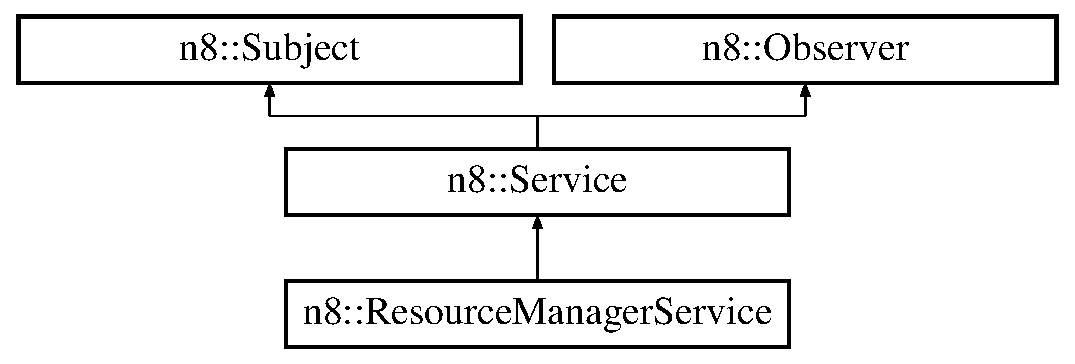
\includegraphics[height=3.000000cm]{classn8_1_1_resource_manager_service}
\end{center}
\end{figure}
\subsection*{Public Member Functions}
\begin{DoxyCompactItemize}
\item 
\hyperlink{classn8_1_1_resource_manager_service_a96e9074b770e268e038daf0d2afb20dc}{Resource\-Manager\-Service} (S\-D\-L\-\_\-\-Surface $\ast$screen)
\item 
\hyperlink{classn8_1_1_resource_manager_service_ac9aea35cebd03445c5bd0bc07e45289c}{$\sim$\-Resource\-Manager\-Service} ()
\item 
void \hyperlink{classn8_1_1_resource_manager_service_ad104d496f6e1dc61ed12895ed9989fe5}{Load\-Images\-From\-File} (std\-::string filepath)
\item 
S\-D\-L\-\_\-\-Surface $\ast$ \hyperlink{classn8_1_1_resource_manager_service_afb39562b3a9448d73eaf5e3041e52011}{Load\-Image} (std\-::string filename)
\item 
void \hyperlink{classn8_1_1_resource_manager_service_a0c5bb1ec14fea9971e8fec2efe8d56cd}{On\-Notify} (\hyperlink{classn8_1_1_event}{Event} $\ast$)
\end{DoxyCompactItemize}
\subsection*{Private Attributes}
\begin{DoxyCompactItemize}
\item 
std\-::map$<$ std\-::string, \\*
S\-D\-L\-\_\-\-Surface $\ast$ $>$ \hyperlink{classn8_1_1_resource_manager_service_af203735b1015f5cf94024e8857c8c17d}{m\-\_\-loaded\-Sprites}
\item 
S\-D\-L\-\_\-\-Surface $\ast$ \hyperlink{classn8_1_1_resource_manager_service_a430459934276e8fd19f5501c04569ab5}{m\-\_\-screen\-Surface}
\end{DoxyCompactItemize}


\subsection{Constructor \& Destructor Documentation}
\hypertarget{classn8_1_1_resource_manager_service_a96e9074b770e268e038daf0d2afb20dc}{\index{n8\-::\-Resource\-Manager\-Service@{n8\-::\-Resource\-Manager\-Service}!Resource\-Manager\-Service@{Resource\-Manager\-Service}}
\index{Resource\-Manager\-Service@{Resource\-Manager\-Service}!n8::ResourceManagerService@{n8\-::\-Resource\-Manager\-Service}}
\subsubsection[{Resource\-Manager\-Service}]{\setlength{\rightskip}{0pt plus 5cm}n8\-::\-Resource\-Manager\-Service\-::\-Resource\-Manager\-Service (
\begin{DoxyParamCaption}
\item[{S\-D\-L\-\_\-\-Surface $\ast$}]{screen}
\end{DoxyParamCaption}
)}}\label{classn8_1_1_resource_manager_service_a96e9074b770e268e038daf0d2afb20dc}
\hypertarget{classn8_1_1_resource_manager_service_ac9aea35cebd03445c5bd0bc07e45289c}{\index{n8\-::\-Resource\-Manager\-Service@{n8\-::\-Resource\-Manager\-Service}!$\sim$\-Resource\-Manager\-Service@{$\sim$\-Resource\-Manager\-Service}}
\index{$\sim$\-Resource\-Manager\-Service@{$\sim$\-Resource\-Manager\-Service}!n8::ResourceManagerService@{n8\-::\-Resource\-Manager\-Service}}
\subsubsection[{$\sim$\-Resource\-Manager\-Service}]{\setlength{\rightskip}{0pt plus 5cm}n8\-::\-Resource\-Manager\-Service\-::$\sim$\-Resource\-Manager\-Service (
\begin{DoxyParamCaption}
{}
\end{DoxyParamCaption}
)}}\label{classn8_1_1_resource_manager_service_ac9aea35cebd03445c5bd0bc07e45289c}
Destructor Deletes all loaded resources 

\subsection{Member Function Documentation}
\hypertarget{classn8_1_1_resource_manager_service_afb39562b3a9448d73eaf5e3041e52011}{\index{n8\-::\-Resource\-Manager\-Service@{n8\-::\-Resource\-Manager\-Service}!Load\-Image@{Load\-Image}}
\index{Load\-Image@{Load\-Image}!n8::ResourceManagerService@{n8\-::\-Resource\-Manager\-Service}}
\subsubsection[{Load\-Image}]{\setlength{\rightskip}{0pt plus 5cm}S\-D\-L\-\_\-\-Surface $\ast$ n8\-::\-Resource\-Manager\-Service\-::\-Load\-Image (
\begin{DoxyParamCaption}
\item[{std\-::string}]{filename}
\end{DoxyParamCaption}
)}}\label{classn8_1_1_resource_manager_service_afb39562b3a9448d73eaf5e3041e52011}
Loads an image from a specified filepath, then creates an optimzed copy of the image


\begin{DoxyParams}{Parameters}
{\em filename} & the filename of the image to load and optimize \\
\hline
\end{DoxyParams}
\begin{DoxyReturn}{Returns}
a pointer to the optimized copy of the image 
\end{DoxyReturn}
\hypertarget{classn8_1_1_resource_manager_service_ad104d496f6e1dc61ed12895ed9989fe5}{\index{n8\-::\-Resource\-Manager\-Service@{n8\-::\-Resource\-Manager\-Service}!Load\-Images\-From\-File@{Load\-Images\-From\-File}}
\index{Load\-Images\-From\-File@{Load\-Images\-From\-File}!n8::ResourceManagerService@{n8\-::\-Resource\-Manager\-Service}}
\subsubsection[{Load\-Images\-From\-File}]{\setlength{\rightskip}{0pt plus 5cm}void n8\-::\-Resource\-Manager\-Service\-::\-Load\-Images\-From\-File (
\begin{DoxyParamCaption}
\item[{std\-::string}]{filepath}
\end{DoxyParamCaption}
)}}\label{classn8_1_1_resource_manager_service_ad104d496f6e1dc61ed12895ed9989fe5}
Parses an input file containing image filepaths, loads those images, and stores them in a map


\begin{DoxyParams}{Parameters}
{\em filepath} & the filepath for the configuration file containing all image filenames to load \\
\hline
\end{DoxyParams}
\hypertarget{classn8_1_1_resource_manager_service_a0c5bb1ec14fea9971e8fec2efe8d56cd}{\index{n8\-::\-Resource\-Manager\-Service@{n8\-::\-Resource\-Manager\-Service}!On\-Notify@{On\-Notify}}
\index{On\-Notify@{On\-Notify}!n8::ResourceManagerService@{n8\-::\-Resource\-Manager\-Service}}
\subsubsection[{On\-Notify}]{\setlength{\rightskip}{0pt plus 5cm}void n8\-::\-Resource\-Manager\-Service\-::\-On\-Notify (
\begin{DoxyParamCaption}
\item[{{\bf n8\-::\-Event} $\ast$}]{event}
\end{DoxyParamCaption}
)\hspace{0.3cm}{\ttfamily [virtual]}}}\label{classn8_1_1_resource_manager_service_a0c5bb1ec14fea9971e8fec2efe8d56cd}


Implements \hyperlink{classn8_1_1_service_a756a170eba7e5c34a1c12008e22d3ca7}{n8\-::\-Service}.



\subsection{Member Data Documentation}
\hypertarget{classn8_1_1_resource_manager_service_af203735b1015f5cf94024e8857c8c17d}{\index{n8\-::\-Resource\-Manager\-Service@{n8\-::\-Resource\-Manager\-Service}!m\-\_\-loaded\-Sprites@{m\-\_\-loaded\-Sprites}}
\index{m\-\_\-loaded\-Sprites@{m\-\_\-loaded\-Sprites}!n8::ResourceManagerService@{n8\-::\-Resource\-Manager\-Service}}
\subsubsection[{m\-\_\-loaded\-Sprites}]{\setlength{\rightskip}{0pt plus 5cm}std\-::map$<$std\-::string,S\-D\-L\-\_\-\-Surface$\ast$$>$ n8\-::\-Resource\-Manager\-Service\-::m\-\_\-loaded\-Sprites\hspace{0.3cm}{\ttfamily [private]}}}\label{classn8_1_1_resource_manager_service_af203735b1015f5cf94024e8857c8c17d}
\hypertarget{classn8_1_1_resource_manager_service_a430459934276e8fd19f5501c04569ab5}{\index{n8\-::\-Resource\-Manager\-Service@{n8\-::\-Resource\-Manager\-Service}!m\-\_\-screen\-Surface@{m\-\_\-screen\-Surface}}
\index{m\-\_\-screen\-Surface@{m\-\_\-screen\-Surface}!n8::ResourceManagerService@{n8\-::\-Resource\-Manager\-Service}}
\subsubsection[{m\-\_\-screen\-Surface}]{\setlength{\rightskip}{0pt plus 5cm}S\-D\-L\-\_\-\-Surface$\ast$ n8\-::\-Resource\-Manager\-Service\-::m\-\_\-screen\-Surface\hspace{0.3cm}{\ttfamily [private]}}}\label{classn8_1_1_resource_manager_service_a430459934276e8fd19f5501c04569ab5}
$<$ Stores all images loaded by the system 

The documentation for this class was generated from the following files\-:\begin{DoxyCompactItemize}
\item 
Services/\hyperlink{_resource_manager_service_8h}{Resource\-Manager\-Service.\-h}\item 
Services/\hyperlink{_resource_manager_service_8cpp}{Resource\-Manager\-Service.\-cpp}\end{DoxyCompactItemize}

\hypertarget{classn8_1_1_service}{\section{n8\-:\-:Service Class Reference}
\label{classn8_1_1_service}\index{n8\-::\-Service@{n8\-::\-Service}}
}


{\ttfamily \#include $<$Service.\-h$>$}

Inheritance diagram for n8\-:\-:Service\-:\begin{figure}[H]
\begin{center}
\leavevmode
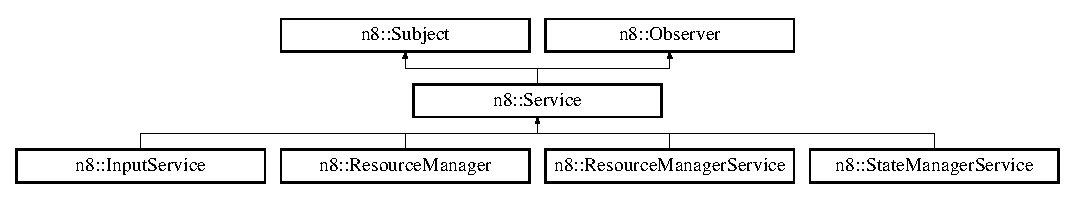
\includegraphics[height=2.222222cm]{classn8_1_1_service}
\end{center}
\end{figure}
\subsection*{Public Member Functions}
\begin{DoxyCompactItemize}
\item 
\hyperlink{classn8_1_1_service_a0f1781fa06e221ff17d2dc1e6e434e22}{Service} ()
\item 
virtual \hyperlink{classn8_1_1_service_a94c2c0b4a5f1da506928db3fe564b917}{$\sim$\-Service} ()
\item 
virtual void \hyperlink{classn8_1_1_service_a756a170eba7e5c34a1c12008e22d3ca7}{On\-Notify} (\hyperlink{classn8_1_1_event}{Event} $\ast$event)=0
\end{DoxyCompactItemize}


\subsection{Constructor \& Destructor Documentation}
\hypertarget{classn8_1_1_service_a0f1781fa06e221ff17d2dc1e6e434e22}{\index{n8\-::\-Service@{n8\-::\-Service}!Service@{Service}}
\index{Service@{Service}!n8::Service@{n8\-::\-Service}}
\subsubsection[{Service}]{\setlength{\rightskip}{0pt plus 5cm}n8\-::\-Service\-::\-Service (
\begin{DoxyParamCaption}
{}
\end{DoxyParamCaption}
)\hspace{0.3cm}{\ttfamily [inline]}}}\label{classn8_1_1_service_a0f1781fa06e221ff17d2dc1e6e434e22}
\hypertarget{classn8_1_1_service_a94c2c0b4a5f1da506928db3fe564b917}{\index{n8\-::\-Service@{n8\-::\-Service}!$\sim$\-Service@{$\sim$\-Service}}
\index{$\sim$\-Service@{$\sim$\-Service}!n8::Service@{n8\-::\-Service}}
\subsubsection[{$\sim$\-Service}]{\setlength{\rightskip}{0pt plus 5cm}n8\-::\-Service\-::$\sim$\-Service (
\begin{DoxyParamCaption}
{}
\end{DoxyParamCaption}
)\hspace{0.3cm}{\ttfamily [inline]}, {\ttfamily [virtual]}}}\label{classn8_1_1_service_a94c2c0b4a5f1da506928db3fe564b917}


\subsection{Member Function Documentation}
\hypertarget{classn8_1_1_service_a756a170eba7e5c34a1c12008e22d3ca7}{\index{n8\-::\-Service@{n8\-::\-Service}!On\-Notify@{On\-Notify}}
\index{On\-Notify@{On\-Notify}!n8::Service@{n8\-::\-Service}}
\subsubsection[{On\-Notify}]{\setlength{\rightskip}{0pt plus 5cm}virtual void n8\-::\-Service\-::\-On\-Notify (
\begin{DoxyParamCaption}
\item[{{\bf Event} $\ast$}]{event}
\end{DoxyParamCaption}
)\hspace{0.3cm}{\ttfamily [pure virtual]}}}\label{classn8_1_1_service_a756a170eba7e5c34a1c12008e22d3ca7}


Implements \hyperlink{classn8_1_1_observer_ab08ada5adb0e21dbb2ee30c26652fd32}{n8\-::\-Observer}.



Implemented in \hyperlink{classn8_1_1_resource_manager_ace97033b439ac0954cf2fc45a79081c9}{n8\-::\-Resource\-Manager}, \hyperlink{classn8_1_1_state_manager_service_a931551f9b6dc470297e9d86abf27b603}{n8\-::\-State\-Manager\-Service}, \hyperlink{classn8_1_1_input_service_aa52767bfd35d3785ea236c8175598212}{n8\-::\-Input\-Service}, and \hyperlink{classn8_1_1_resource_manager_service_a0c5bb1ec14fea9971e8fec2efe8d56cd}{n8\-::\-Resource\-Manager\-Service}.



The documentation for this class was generated from the following files\-:\begin{DoxyCompactItemize}
\item 
Base/\hyperlink{_service_8h}{Service.\-h}\item 
Base/\hyperlink{_service_8cpp}{Service.\-cpp}\end{DoxyCompactItemize}

\hypertarget{classn8_1_1_service_manager}{\section{n8\-:\-:Service\-Manager Class Reference}
\label{classn8_1_1_service_manager}\index{n8\-::\-Service\-Manager@{n8\-::\-Service\-Manager}}
}


{\ttfamily \#include $<$Service\-Manager.\-h$>$}

Inheritance diagram for n8\-:\-:Service\-Manager\-:\begin{figure}[H]
\begin{center}
\leavevmode
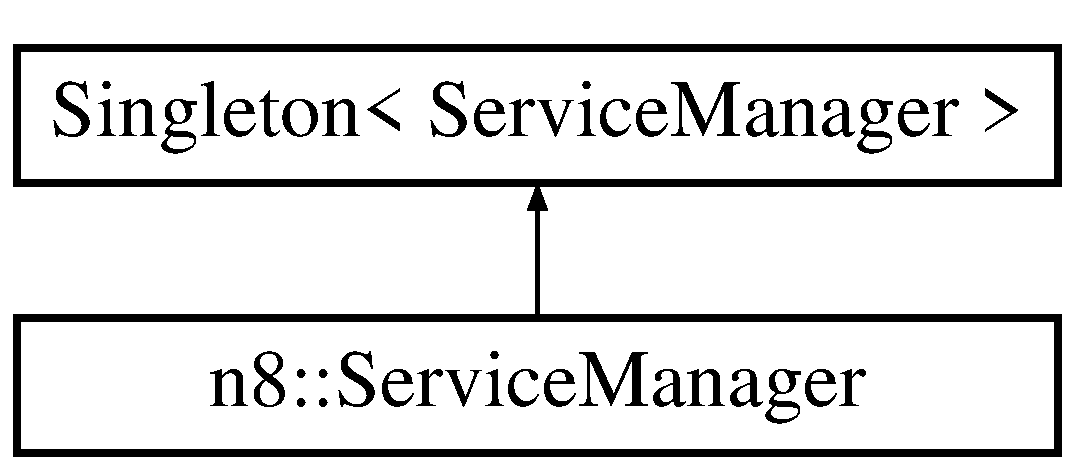
\includegraphics[height=2.000000cm]{classn8_1_1_service_manager}
\end{center}
\end{figure}
\subsection*{Public Member Functions}
\begin{DoxyCompactItemize}
\item 
\hyperlink{classn8_1_1_service_manager_abfe06bc245147f48eca750686d9e1ca0}{Service\-Manager} ()
\item 
\hyperlink{classn8_1_1_service_manager_a329524860b322f5a3ba6ac0b5f909cd8}{$\sim$\-Service\-Manager} ()
\item 
void \hyperlink{classn8_1_1_service_manager_ae3bbc7dc34aa6e747eb301c7935039ab}{Register\-Service} (\hyperlink{namespace_e_service_a7d0bb3de6ea857dc1253fc5a2cef6884}{E\-Service\-::\-Values}, \hyperlink{classn8_1_1_service}{Service} $\ast$)
\item 
void \hyperlink{classn8_1_1_service_manager_a1309152e05c95e60cf98600b9e3053c6}{Unregister\-Service} (\hyperlink{namespace_e_service_a7d0bb3de6ea857dc1253fc5a2cef6884}{E\-Service\-::\-Values})
\item 
void \hyperlink{classn8_1_1_service_manager_a56b16c5856e36f9765029bdbb802bc18}{Remove\-All\-Services} ()
\item 
\hyperlink{classn8_1_1_service}{Service} $\ast$ \hyperlink{classn8_1_1_service_manager_a050b710ab08a641c6562898409afae02}{Get\-Service} (\hyperlink{namespace_e_service_a7d0bb3de6ea857dc1253fc5a2cef6884}{E\-Service\-::\-Values})
\end{DoxyCompactItemize}
\subsection*{Private Attributes}
\begin{DoxyCompactItemize}
\item 
std\-::map$<$ \hyperlink{namespace_e_service_a7d0bb3de6ea857dc1253fc5a2cef6884}{E\-Service\-::\-Values}, \\*
\hyperlink{classn8_1_1_service}{Service} $\ast$ $>$ \hyperlink{classn8_1_1_service_manager_a631c25768aaa053b06aa519fc8a00d65}{m\-\_\-registered\-Services}
\end{DoxyCompactItemize}
\subsection*{Additional Inherited Members}


\subsection{Detailed Description}
Provides a global access point to registered services. This gives a less coupled way of providing access to game systems. Services are registered with the \hyperlink{classn8_1_1_service_manager}{Service\-Manager} during the game's initialization. 

\subsection{Constructor \& Destructor Documentation}
\hypertarget{classn8_1_1_service_manager_abfe06bc245147f48eca750686d9e1ca0}{\index{n8\-::\-Service\-Manager@{n8\-::\-Service\-Manager}!Service\-Manager@{Service\-Manager}}
\index{Service\-Manager@{Service\-Manager}!n8::ServiceManager@{n8\-::\-Service\-Manager}}
\subsubsection[{Service\-Manager}]{\setlength{\rightskip}{0pt plus 5cm}n8\-::\-Service\-Manager\-::\-Service\-Manager (
\begin{DoxyParamCaption}
{}
\end{DoxyParamCaption}
)}}\label{classn8_1_1_service_manager_abfe06bc245147f48eca750686d9e1ca0}
Default Constructor \hypertarget{classn8_1_1_service_manager_a329524860b322f5a3ba6ac0b5f909cd8}{\index{n8\-::\-Service\-Manager@{n8\-::\-Service\-Manager}!$\sim$\-Service\-Manager@{$\sim$\-Service\-Manager}}
\index{$\sim$\-Service\-Manager@{$\sim$\-Service\-Manager}!n8::ServiceManager@{n8\-::\-Service\-Manager}}
\subsubsection[{$\sim$\-Service\-Manager}]{\setlength{\rightskip}{0pt plus 5cm}n8\-::\-Service\-Manager\-::$\sim$\-Service\-Manager (
\begin{DoxyParamCaption}
{}
\end{DoxyParamCaption}
)}}\label{classn8_1_1_service_manager_a329524860b322f5a3ba6ac0b5f909cd8}
Destructor 

\subsection{Member Function Documentation}
\hypertarget{classn8_1_1_service_manager_a050b710ab08a641c6562898409afae02}{\index{n8\-::\-Service\-Manager@{n8\-::\-Service\-Manager}!Get\-Service@{Get\-Service}}
\index{Get\-Service@{Get\-Service}!n8::ServiceManager@{n8\-::\-Service\-Manager}}
\subsubsection[{Get\-Service}]{\setlength{\rightskip}{0pt plus 5cm}{\bf n8\-::\-Service} $\ast$ n8\-::\-Service\-Manager\-::\-Get\-Service (
\begin{DoxyParamCaption}
\item[{{\bf E\-Service\-::\-Values}}]{key}
\end{DoxyParamCaption}
)}}\label{classn8_1_1_service_manager_a050b710ab08a641c6562898409afae02}
Get\-Service Returns the service specified by the input key


\begin{DoxyParams}{Parameters}
{\em \hyperlink{namespace_e_service}{E\-Service}} & An enum value to use as the lookup key for the map \\
\hline
\end{DoxyParams}
\hypertarget{classn8_1_1_service_manager_ae3bbc7dc34aa6e747eb301c7935039ab}{\index{n8\-::\-Service\-Manager@{n8\-::\-Service\-Manager}!Register\-Service@{Register\-Service}}
\index{Register\-Service@{Register\-Service}!n8::ServiceManager@{n8\-::\-Service\-Manager}}
\subsubsection[{Register\-Service}]{\setlength{\rightskip}{0pt plus 5cm}void n8\-::\-Service\-Manager\-::\-Register\-Service (
\begin{DoxyParamCaption}
\item[{{\bf E\-Service\-::\-Values}}]{key, }
\item[{{\bf Service} $\ast$}]{new\-Service}
\end{DoxyParamCaption}
)}}\label{classn8_1_1_service_manager_ae3bbc7dc34aa6e747eb301c7935039ab}
Register\-Service Registers a provided service by adding it to a map of registered services using a provided enum value as a key.


\begin{DoxyParams}{Parameters}
{\em \hyperlink{namespace_e_service}{E\-Service}} & An enum value to use as a map key \\
\hline
{\em Service$\ast$} & A pointer to a new service \\
\hline
\end{DoxyParams}
\hypertarget{classn8_1_1_service_manager_a56b16c5856e36f9765029bdbb802bc18}{\index{n8\-::\-Service\-Manager@{n8\-::\-Service\-Manager}!Remove\-All\-Services@{Remove\-All\-Services}}
\index{Remove\-All\-Services@{Remove\-All\-Services}!n8::ServiceManager@{n8\-::\-Service\-Manager}}
\subsubsection[{Remove\-All\-Services}]{\setlength{\rightskip}{0pt plus 5cm}void n8\-::\-Service\-Manager\-::\-Remove\-All\-Services (
\begin{DoxyParamCaption}
{}
\end{DoxyParamCaption}
)}}\label{classn8_1_1_service_manager_a56b16c5856e36f9765029bdbb802bc18}
Remove\-All\-Services Removes and deletes all services from the map \hypertarget{classn8_1_1_service_manager_a1309152e05c95e60cf98600b9e3053c6}{\index{n8\-::\-Service\-Manager@{n8\-::\-Service\-Manager}!Unregister\-Service@{Unregister\-Service}}
\index{Unregister\-Service@{Unregister\-Service}!n8::ServiceManager@{n8\-::\-Service\-Manager}}
\subsubsection[{Unregister\-Service}]{\setlength{\rightskip}{0pt plus 5cm}void n8\-::\-Service\-Manager\-::\-Unregister\-Service (
\begin{DoxyParamCaption}
\item[{{\bf E\-Service\-::\-Values}}]{key}
\end{DoxyParamCaption}
)}}\label{classn8_1_1_service_manager_a1309152e05c95e60cf98600b9e3053c6}
Unregister\-Service Unregisters a service by removing it from the map


\begin{DoxyParams}{Parameters}
{\em \hyperlink{namespace_e_service}{E\-Service}} & An enum value to use as a map key \\
\hline
\end{DoxyParams}


\subsection{Member Data Documentation}
\hypertarget{classn8_1_1_service_manager_a631c25768aaa053b06aa519fc8a00d65}{\index{n8\-::\-Service\-Manager@{n8\-::\-Service\-Manager}!m\-\_\-registered\-Services@{m\-\_\-registered\-Services}}
\index{m\-\_\-registered\-Services@{m\-\_\-registered\-Services}!n8::ServiceManager@{n8\-::\-Service\-Manager}}
\subsubsection[{m\-\_\-registered\-Services}]{\setlength{\rightskip}{0pt plus 5cm}std\-::map$<${\bf E\-Service\-::\-Values},{\bf Service}$\ast$$>$ n8\-::\-Service\-Manager\-::m\-\_\-registered\-Services\hspace{0.3cm}{\ttfamily [private]}}}\label{classn8_1_1_service_manager_a631c25768aaa053b06aa519fc8a00d65}


The documentation for this class was generated from the following files\-:\begin{DoxyCompactItemize}
\item 
Core/\hyperlink{_service_manager_8h}{Service\-Manager.\-h}\item 
Core/\hyperlink{_service_manager_8cpp}{Service\-Manager.\-cpp}\end{DoxyCompactItemize}

\hypertarget{class_singleton}{\section{Singleton$<$ T $>$ Class Template Reference}
\label{class_singleton}\index{Singleton$<$ T $>$@{Singleton$<$ T $>$}}
}


{\ttfamily \#include $<$Singleton.\-h$>$}

\subsection*{Static Public Member Functions}
\begin{DoxyCompactItemize}
\item 
static T $\ast$ \hyperlink{class_singleton_a9460c2b31ff4dd9f7d022b0fff0afda4}{Get\-Instance} ()
\item 
static void \hyperlink{class_singleton_a3cf263c9304948f53b8a4e8082761930}{Create} ()
\item 
static void \hyperlink{class_singleton_a7058846441886b854787967b56c088dc}{Destroy} ()
\end{DoxyCompactItemize}
\subsection*{Static Protected Attributes}
\begin{DoxyCompactItemize}
\item 
static T $\ast$ \hyperlink{class_singleton_a77987e85742da3505825c3195ed7c8a6}{m\-\_\-instance} = 0
\end{DoxyCompactItemize}


\subsection{Member Function Documentation}
\hypertarget{class_singleton_a3cf263c9304948f53b8a4e8082761930}{\index{Singleton@{Singleton}!Create@{Create}}
\index{Create@{Create}!Singleton@{Singleton}}
\subsubsection[{Create}]{\setlength{\rightskip}{0pt plus 5cm}template$<$class T$>$ static void {\bf Singleton}$<$ T $>$\-::Create (
\begin{DoxyParamCaption}
{}
\end{DoxyParamCaption}
)\hspace{0.3cm}{\ttfamily [inline]}, {\ttfamily [static]}}}\label{class_singleton_a3cf263c9304948f53b8a4e8082761930}
\hypertarget{class_singleton_a7058846441886b854787967b56c088dc}{\index{Singleton@{Singleton}!Destroy@{Destroy}}
\index{Destroy@{Destroy}!Singleton@{Singleton}}
\subsubsection[{Destroy}]{\setlength{\rightskip}{0pt plus 5cm}template$<$class T$>$ static void {\bf Singleton}$<$ T $>$\-::Destroy (
\begin{DoxyParamCaption}
{}
\end{DoxyParamCaption}
)\hspace{0.3cm}{\ttfamily [inline]}, {\ttfamily [static]}}}\label{class_singleton_a7058846441886b854787967b56c088dc}
\hypertarget{class_singleton_a9460c2b31ff4dd9f7d022b0fff0afda4}{\index{Singleton@{Singleton}!Get\-Instance@{Get\-Instance}}
\index{Get\-Instance@{Get\-Instance}!Singleton@{Singleton}}
\subsubsection[{Get\-Instance}]{\setlength{\rightskip}{0pt plus 5cm}template$<$class T$>$ static T$\ast$ {\bf Singleton}$<$ T $>$\-::Get\-Instance (
\begin{DoxyParamCaption}
{}
\end{DoxyParamCaption}
)\hspace{0.3cm}{\ttfamily [inline]}, {\ttfamily [static]}}}\label{class_singleton_a9460c2b31ff4dd9f7d022b0fff0afda4}


\subsection{Member Data Documentation}
\hypertarget{class_singleton_a77987e85742da3505825c3195ed7c8a6}{\index{Singleton@{Singleton}!m\-\_\-instance@{m\-\_\-instance}}
\index{m\-\_\-instance@{m\-\_\-instance}!Singleton@{Singleton}}
\subsubsection[{m\-\_\-instance}]{\setlength{\rightskip}{0pt plus 5cm}template$<$class T$>$ T $\ast$ {\bf Singleton}$<$ T $>$\-::m\-\_\-instance = 0\hspace{0.3cm}{\ttfamily [static]}, {\ttfamily [protected]}}}\label{class_singleton_a77987e85742da3505825c3195ed7c8a6}


The documentation for this class was generated from the following file\-:\begin{DoxyCompactItemize}
\item 
Base/\hyperlink{_singleton_8h}{Singleton.\-h}\end{DoxyCompactItemize}

\hypertarget{classn8_1_1_sound_effect}{\section{n8\-:\-:Sound\-Effect Class Reference}
\label{classn8_1_1_sound_effect}\index{n8\-::\-Sound\-Effect@{n8\-::\-Sound\-Effect}}
}


{\ttfamily \#include $<$Sound\-Effect.\-h$>$}

Inheritance diagram for n8\-:\-:Sound\-Effect\-:\begin{figure}[H]
\begin{center}
\leavevmode
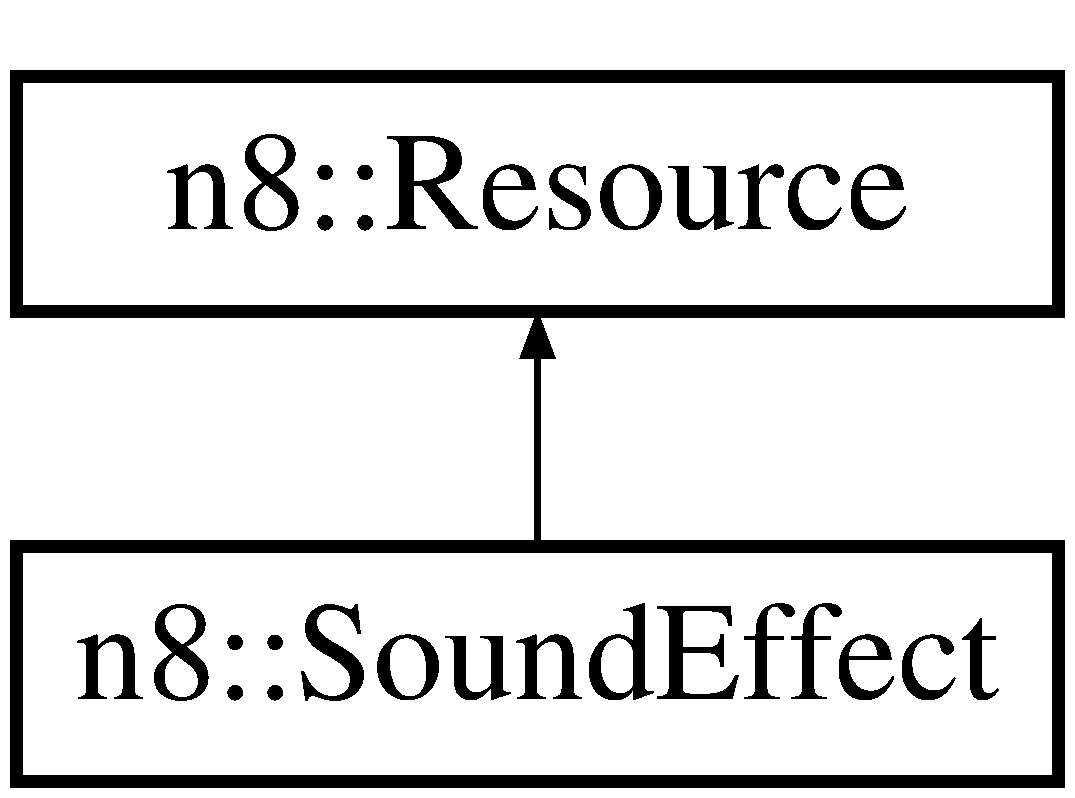
\includegraphics[height=2.000000cm]{classn8_1_1_sound_effect}
\end{center}
\end{figure}
\subsection*{Public Member Functions}
\begin{DoxyCompactItemize}
\item 
\hyperlink{classn8_1_1_sound_effect_a9c5c649a5ea25826ea5f3171df2d8dee}{Sound\-Effect} (std\-::string p\-\_\-id, Mix\-\_\-\-Chunk $\ast$p\-\_\-mix\-Chunk)
\item 
\hyperlink{classn8_1_1_sound_effect_adb0887888f815d5796a20a1e515d1592}{$\sim$\-Sound\-Effect} ()
\end{DoxyCompactItemize}
\subsection*{Private Attributes}
\begin{DoxyCompactItemize}
\item 
Mix\-\_\-\-Chunk $\ast$ \hyperlink{classn8_1_1_sound_effect_a5faa9a06016c7cef864ccb8d27740a33}{m\-\_\-sound\-Effect}
\end{DoxyCompactItemize}
\subsection*{Friends}
\begin{DoxyCompactItemize}
\item 
class \hyperlink{classn8_1_1_sound_effect_a37b580cb33a7b41e459ef8adf3e2dd75}{Audio\-Service}
\end{DoxyCompactItemize}


\subsection{Constructor \& Destructor Documentation}
\hypertarget{classn8_1_1_sound_effect_a9c5c649a5ea25826ea5f3171df2d8dee}{\index{n8\-::\-Sound\-Effect@{n8\-::\-Sound\-Effect}!Sound\-Effect@{Sound\-Effect}}
\index{Sound\-Effect@{Sound\-Effect}!n8::SoundEffect@{n8\-::\-Sound\-Effect}}
\subsubsection[{Sound\-Effect}]{\setlength{\rightskip}{0pt plus 5cm}n8\-::\-Sound\-Effect\-::\-Sound\-Effect (
\begin{DoxyParamCaption}
\item[{std\-::string}]{p\-\_\-id, }
\item[{Mix\-\_\-\-Chunk $\ast$}]{p\-\_\-mix\-Chunk}
\end{DoxyParamCaption}
)}}\label{classn8_1_1_sound_effect_a9c5c649a5ea25826ea5f3171df2d8dee}
\hypertarget{classn8_1_1_sound_effect_adb0887888f815d5796a20a1e515d1592}{\index{n8\-::\-Sound\-Effect@{n8\-::\-Sound\-Effect}!$\sim$\-Sound\-Effect@{$\sim$\-Sound\-Effect}}
\index{$\sim$\-Sound\-Effect@{$\sim$\-Sound\-Effect}!n8::SoundEffect@{n8\-::\-Sound\-Effect}}
\subsubsection[{$\sim$\-Sound\-Effect}]{\setlength{\rightskip}{0pt plus 5cm}n8\-::\-Sound\-Effect\-::$\sim$\-Sound\-Effect (
\begin{DoxyParamCaption}
{}
\end{DoxyParamCaption}
)}}\label{classn8_1_1_sound_effect_adb0887888f815d5796a20a1e515d1592}


\subsection{Friends And Related Function Documentation}
\hypertarget{classn8_1_1_sound_effect_a37b580cb33a7b41e459ef8adf3e2dd75}{\index{n8\-::\-Sound\-Effect@{n8\-::\-Sound\-Effect}!Audio\-Service@{Audio\-Service}}
\index{Audio\-Service@{Audio\-Service}!n8::SoundEffect@{n8\-::\-Sound\-Effect}}
\subsubsection[{Audio\-Service}]{\setlength{\rightskip}{0pt plus 5cm}friend class Audio\-Service\hspace{0.3cm}{\ttfamily [friend]}}}\label{classn8_1_1_sound_effect_a37b580cb33a7b41e459ef8adf3e2dd75}


\subsection{Member Data Documentation}
\hypertarget{classn8_1_1_sound_effect_a5faa9a06016c7cef864ccb8d27740a33}{\index{n8\-::\-Sound\-Effect@{n8\-::\-Sound\-Effect}!m\-\_\-sound\-Effect@{m\-\_\-sound\-Effect}}
\index{m\-\_\-sound\-Effect@{m\-\_\-sound\-Effect}!n8::SoundEffect@{n8\-::\-Sound\-Effect}}
\subsubsection[{m\-\_\-sound\-Effect}]{\setlength{\rightskip}{0pt plus 5cm}Mix\-\_\-\-Chunk$\ast$ n8\-::\-Sound\-Effect\-::m\-\_\-sound\-Effect\hspace{0.3cm}{\ttfamily [private]}}}\label{classn8_1_1_sound_effect_a5faa9a06016c7cef864ccb8d27740a33}


The documentation for this class was generated from the following files\-:\begin{DoxyCompactItemize}
\item 
Resources/\hyperlink{_sound_effect_8h}{Sound\-Effect.\-h}\item 
Resources/\hyperlink{_sound_effect_8cpp}{Sound\-Effect.\-cpp}\end{DoxyCompactItemize}

\hypertarget{classn8_1_1_sprite}{\section{n8\-:\-:Sprite Class Reference}
\label{classn8_1_1_sprite}\index{n8\-::\-Sprite@{n8\-::\-Sprite}}
}


{\ttfamily \#include $<$Sprite.\-h$>$}

Inheritance diagram for n8\-:\-:Sprite\-:\begin{figure}[H]
\begin{center}
\leavevmode
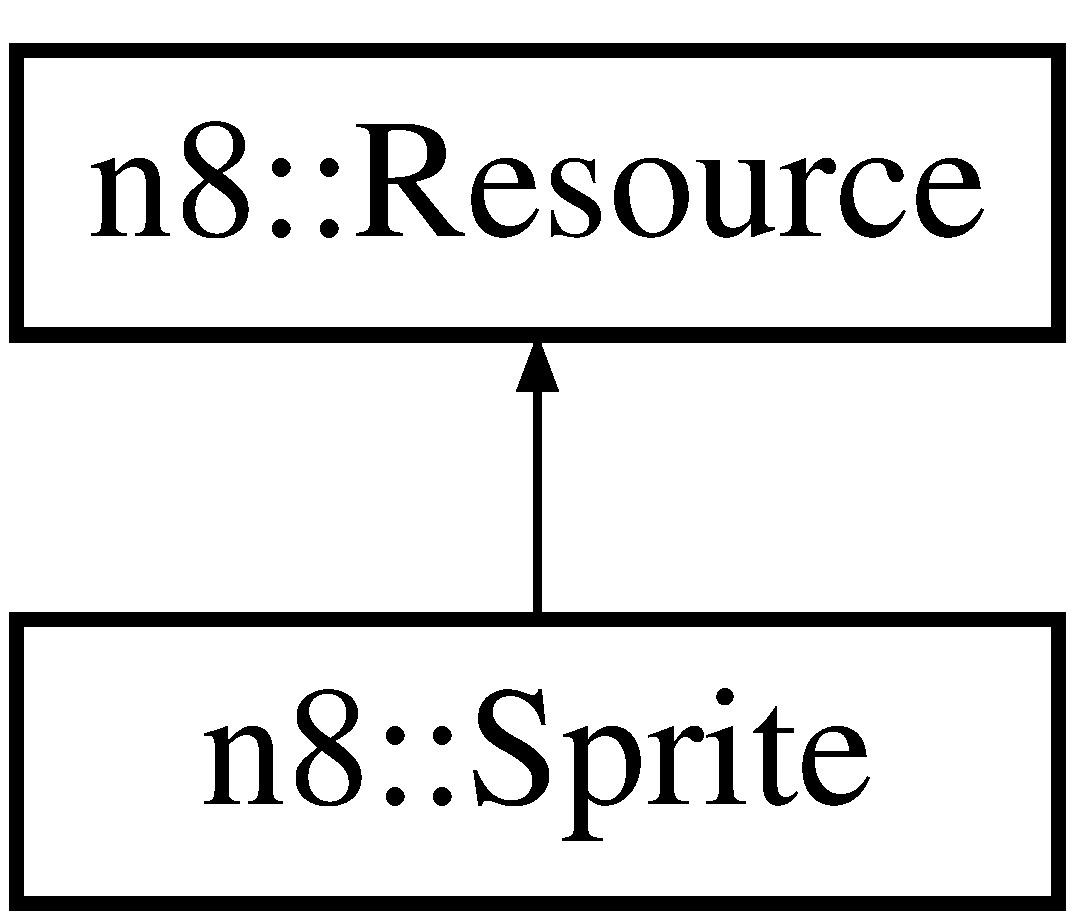
\includegraphics[height=2.000000cm]{classn8_1_1_sprite}
\end{center}
\end{figure}
\subsection*{Public Member Functions}
\begin{DoxyCompactItemize}
\item 
\hyperlink{classn8_1_1_sprite_a6cbe9ac58c5f03c898b8247b96852769}{$\sim$\-Sprite} ()
\item 
\hyperlink{classn8_1_1_sprite_a8c20ff646bf175ed1419bf85dac7368f}{Sprite} (std\-::string p\-\_\-id, S\-D\-L\-\_\-\-Surface $\ast$p\-\_\-img)
\item 
int \hyperlink{classn8_1_1_sprite_a7de2553c07f843b8fd6a1431342e463f}{Get\-Height} ()
\item 
int \hyperlink{classn8_1_1_sprite_a683b19b12bc8d3b655598666200b1387}{Get\-Width} ()
\item 
bool \hyperlink{classn8_1_1_sprite_a54005df4d27a045f844b0074b5e1b119}{Draw} (int p\-\_\-x, int p\-\_\-y, S\-D\-L\-\_\-\-Surface $\ast$p\-\_\-destination)
\item 
bool \hyperlink{classn8_1_1_sprite_a074384ce9bc2c0a5c7740c1d8faeb501}{Draw} (int p\-\_\-x, int p\-\_\-y, int p\-\_\-x2, int p\-\_\-y2, int p\-\_\-width, int p\-\_\-height, S\-D\-L\-\_\-\-Surface $\ast$p\-\_\-dest)
\end{DoxyCompactItemize}
\subsection*{Private Attributes}
\begin{DoxyCompactItemize}
\item 
S\-D\-L\-\_\-\-Surface $\ast$ \hyperlink{classn8_1_1_sprite_a8bbf98f385191ab5d756784ceac802b1}{m\-\_\-image}
\end{DoxyCompactItemize}
\subsection*{Friends}
\begin{DoxyCompactItemize}
\item 
class \hyperlink{classn8_1_1_sprite_aedde775898ebe0d7c84c0060e1c9d770}{Render\-Service}
\end{DoxyCompactItemize}


\subsection{Detailed Description}
An object to hold an optimzed S\-D\-L\-\_\-\-Surface image and provide access to it 

\subsection{Constructor \& Destructor Documentation}
\hypertarget{classn8_1_1_sprite_a6cbe9ac58c5f03c898b8247b96852769}{\index{n8\-::\-Sprite@{n8\-::\-Sprite}!$\sim$\-Sprite@{$\sim$\-Sprite}}
\index{$\sim$\-Sprite@{$\sim$\-Sprite}!n8::Sprite@{n8\-::\-Sprite}}
\subsubsection[{$\sim$\-Sprite}]{\setlength{\rightskip}{0pt plus 5cm}n8\-::\-Sprite\-::$\sim$\-Sprite (
\begin{DoxyParamCaption}
{}
\end{DoxyParamCaption}
)}}\label{classn8_1_1_sprite_a6cbe9ac58c5f03c898b8247b96852769}
Default Destructor 

Frees the loaded S\-D\-L\-\_\-\-Surface which is pointed to by image\-\_\- \hypertarget{classn8_1_1_sprite_a8c20ff646bf175ed1419bf85dac7368f}{\index{n8\-::\-Sprite@{n8\-::\-Sprite}!Sprite@{Sprite}}
\index{Sprite@{Sprite}!n8::Sprite@{n8\-::\-Sprite}}
\subsubsection[{Sprite}]{\setlength{\rightskip}{0pt plus 5cm}n8\-::\-Sprite\-::\-Sprite (
\begin{DoxyParamCaption}
\item[{std\-::string}]{p\-\_\-id, }
\item[{S\-D\-L\-\_\-\-Surface $\ast$}]{p\-\_\-img}
\end{DoxyParamCaption}
)}}\label{classn8_1_1_sprite_a8c20ff646bf175ed1419bf85dac7368f}
Constructor 

Initializes id\-\_\- and image\-\_\- to passed values


\begin{DoxyParams}{Parameters}
{\em id} & The unique identifier for the sprite. \\
\hline
{\em img} & The S\-D\-L\-\_\-\-Surface to store in the sprite object \\
\hline
\end{DoxyParams}


\subsection{Member Function Documentation}
\hypertarget{classn8_1_1_sprite_a54005df4d27a045f844b0074b5e1b119}{\index{n8\-::\-Sprite@{n8\-::\-Sprite}!Draw@{Draw}}
\index{Draw@{Draw}!n8::Sprite@{n8\-::\-Sprite}}
\subsubsection[{Draw}]{\setlength{\rightskip}{0pt plus 5cm}bool n8\-::\-Sprite\-::\-Draw (
\begin{DoxyParamCaption}
\item[{int}]{p\-\_\-x, }
\item[{int}]{p\-\_\-y, }
\item[{S\-D\-L\-\_\-\-Surface $\ast$}]{p\-\_\-destination}
\end{DoxyParamCaption}
)}}\label{classn8_1_1_sprite_a54005df4d27a045f844b0074b5e1b119}
Draws the sprite image to a destination S\-D\-L\-\_\-\-Surface.


\begin{DoxyParams}{Parameters}
{\em x} & The x location where the source S\-D\-L\-\_\-\-Surface should be drawn \\
\hline
{\em y} & The y location where the source S\-D\-L\-\_\-\-Surface should be drawn \\
\hline
{\em destination} & The canvas S\-D\-L\-\_\-\-Surface that images are drawn to \\
\hline
\end{DoxyParams}
\hypertarget{classn8_1_1_sprite_a074384ce9bc2c0a5c7740c1d8faeb501}{\index{n8\-::\-Sprite@{n8\-::\-Sprite}!Draw@{Draw}}
\index{Draw@{Draw}!n8::Sprite@{n8\-::\-Sprite}}
\subsubsection[{Draw}]{\setlength{\rightskip}{0pt plus 5cm}bool n8\-::\-Sprite\-::\-Draw (
\begin{DoxyParamCaption}
\item[{int}]{p\-\_\-x, }
\item[{int}]{p\-\_\-y, }
\item[{int}]{p\-\_\-x2, }
\item[{int}]{p\-\_\-y2, }
\item[{int}]{p\-\_\-width, }
\item[{int}]{p\-\_\-height, }
\item[{S\-D\-L\-\_\-\-Surface $\ast$}]{p\-\_\-destination}
\end{DoxyParamCaption}
)}}\label{classn8_1_1_sprite_a074384ce9bc2c0a5c7740c1d8faeb501}
Used to draw a section of the sprite image to the screen. The size of the sub-\/image is given along with the coordinates in the source image to take the sub image from. Specifying x2 = 0, y2=0, width = 50, height=50 would take the top left 50x50 portion of the source image.


\begin{DoxyParams}{Parameters}
{\em x} & The x location where the sub-\/image should be drawn \\
\hline
{\em y} & The y location where the sub-\/image should be drawn \\
\hline
{\em x2} & The x location for the sub-\/image to be taken from the source image \\
\hline
{\em y2} & The y location for the sub-\/image to be taken from the source image \\
\hline
{\em width} & The width of the sub-\/image \\
\hline
{\em height} & The height of the sub-\/image \\
\hline
{\em destination} & The canvas S\-D\-L\-\_\-\-Surface that images are drawn to \\
\hline
\end{DoxyParams}
\hypertarget{classn8_1_1_sprite_a7de2553c07f843b8fd6a1431342e463f}{\index{n8\-::\-Sprite@{n8\-::\-Sprite}!Get\-Height@{Get\-Height}}
\index{Get\-Height@{Get\-Height}!n8::Sprite@{n8\-::\-Sprite}}
\subsubsection[{Get\-Height}]{\setlength{\rightskip}{0pt plus 5cm}int n8\-::\-Sprite\-::\-Get\-Height (
\begin{DoxyParamCaption}
{}
\end{DoxyParamCaption}
)\hspace{0.3cm}{\ttfamily [inline]}}}\label{classn8_1_1_sprite_a7de2553c07f843b8fd6a1431342e463f}
\begin{DoxyVerb}Used to get the image stored in the sprite so it can be drawn to the screen
\end{DoxyVerb}


\begin{DoxyReturn}{Returns}
The S\-D\-L\-\_\-\-Surface stored with image\-\_\-
\end{DoxyReturn}
S\-D\-L\-\_\-\-Surface$\ast$ get\-\_\-image() \{return m\-\_\-image;\}Used to get the height of the sprite image

\begin{DoxyReturn}{Returns}
The height of the S\-D\-L\-\_\-\-Surface referenced by image\-\_\- 
\end{DoxyReturn}
\hypertarget{classn8_1_1_sprite_a683b19b12bc8d3b655598666200b1387}{\index{n8\-::\-Sprite@{n8\-::\-Sprite}!Get\-Width@{Get\-Width}}
\index{Get\-Width@{Get\-Width}!n8::Sprite@{n8\-::\-Sprite}}
\subsubsection[{Get\-Width}]{\setlength{\rightskip}{0pt plus 5cm}int n8\-::\-Sprite\-::\-Get\-Width (
\begin{DoxyParamCaption}
{}
\end{DoxyParamCaption}
)\hspace{0.3cm}{\ttfamily [inline]}}}\label{classn8_1_1_sprite_a683b19b12bc8d3b655598666200b1387}
Used to get the width of the sprite image

\begin{DoxyReturn}{Returns}
The width of the S\-D\-L\-\_\-\-Surface referenced by image\-\_\- 
\end{DoxyReturn}


\subsection{Friends And Related Function Documentation}
\hypertarget{classn8_1_1_sprite_aedde775898ebe0d7c84c0060e1c9d770}{\index{n8\-::\-Sprite@{n8\-::\-Sprite}!Render\-Service@{Render\-Service}}
\index{Render\-Service@{Render\-Service}!n8::Sprite@{n8\-::\-Sprite}}
\subsubsection[{Render\-Service}]{\setlength{\rightskip}{0pt plus 5cm}friend class Render\-Service\hspace{0.3cm}{\ttfamily [friend]}}}\label{classn8_1_1_sprite_aedde775898ebe0d7c84c0060e1c9d770}
$<$ The image that can be drawn to a canvas 

\subsection{Member Data Documentation}
\hypertarget{classn8_1_1_sprite_a8bbf98f385191ab5d756784ceac802b1}{\index{n8\-::\-Sprite@{n8\-::\-Sprite}!m\-\_\-image@{m\-\_\-image}}
\index{m\-\_\-image@{m\-\_\-image}!n8::Sprite@{n8\-::\-Sprite}}
\subsubsection[{m\-\_\-image}]{\setlength{\rightskip}{0pt plus 5cm}S\-D\-L\-\_\-\-Surface$\ast$ n8\-::\-Sprite\-::m\-\_\-image\hspace{0.3cm}{\ttfamily [private]}}}\label{classn8_1_1_sprite_a8bbf98f385191ab5d756784ceac802b1}


The documentation for this class was generated from the following files\-:\begin{DoxyCompactItemize}
\item 
Resources/\hyperlink{_sprite_8h}{Sprite.\-h}\item 
Resources/\hyperlink{_sprite_8cpp}{Sprite.\-cpp}\end{DoxyCompactItemize}

\hypertarget{classn8_1_1_state}{\section{n8\-:\-:State Class Reference}
\label{classn8_1_1_state}\index{n8\-::\-State@{n8\-::\-State}}
}


{\ttfamily \#include $<$State.\-h$>$}

\subsection*{Public Member Functions}
\begin{DoxyCompactItemize}
\item 
\hyperlink{class_i_d}{I\-D} \hyperlink{classn8_1_1_state_adbb6b659c390b191bb61f0e160e93eec}{Get\-Id} ()
\item 
virtual void \hyperlink{classn8_1_1_state_acbd41cd50cb1238068cb758862369797}{On\-Resume} ()=0
\item 
virtual void \hyperlink{classn8_1_1_state_a0ba47df708916069474719d872a78481}{On\-Pause} ()=0
\item 
virtual void \hyperlink{classn8_1_1_state_a4a881caf4314fb528f82ad974ad26ef7}{Update} (Uint32 current\-Time)=0
\item 
virtual void \hyperlink{classn8_1_1_state_a1ec9371023ca55c020727a6b49167a91}{Render} (S\-D\-L\-\_\-\-Window $\ast$window)=0
\end{DoxyCompactItemize}
\subsection*{Protected Attributes}
\begin{DoxyCompactItemize}
\item 
Uint32 \hyperlink{classn8_1_1_state_ab8ef61270130e480fd946b62badd6123}{m\-\_\-time}
\item 
\hyperlink{class_i_d}{I\-D} $\ast$ \hyperlink{classn8_1_1_state_a1029f2fda72e7e50369d48f4c9641843}{m\-\_\-id}
\end{DoxyCompactItemize}


\subsection{Detailed Description}
Base class for game states 

\subsection{Member Function Documentation}
\hypertarget{classn8_1_1_state_adbb6b659c390b191bb61f0e160e93eec}{\index{n8\-::\-State@{n8\-::\-State}!Get\-Id@{Get\-Id}}
\index{Get\-Id@{Get\-Id}!n8::State@{n8\-::\-State}}
\subsubsection[{Get\-Id}]{\setlength{\rightskip}{0pt plus 5cm}{\bf I\-D} n8\-::\-State\-::\-Get\-Id (
\begin{DoxyParamCaption}
{}
\end{DoxyParamCaption}
)\hspace{0.3cm}{\ttfamily [inline]}}}\label{classn8_1_1_state_adbb6b659c390b191bb61f0e160e93eec}
\hypertarget{classn8_1_1_state_a0ba47df708916069474719d872a78481}{\index{n8\-::\-State@{n8\-::\-State}!On\-Pause@{On\-Pause}}
\index{On\-Pause@{On\-Pause}!n8::State@{n8\-::\-State}}
\subsubsection[{On\-Pause}]{\setlength{\rightskip}{0pt plus 5cm}virtual void n8\-::\-State\-::\-On\-Pause (
\begin{DoxyParamCaption}
{}
\end{DoxyParamCaption}
)\hspace{0.3cm}{\ttfamily [pure virtual]}}}\label{classn8_1_1_state_a0ba47df708916069474719d872a78481}
\hypertarget{classn8_1_1_state_acbd41cd50cb1238068cb758862369797}{\index{n8\-::\-State@{n8\-::\-State}!On\-Resume@{On\-Resume}}
\index{On\-Resume@{On\-Resume}!n8::State@{n8\-::\-State}}
\subsubsection[{On\-Resume}]{\setlength{\rightskip}{0pt plus 5cm}virtual void n8\-::\-State\-::\-On\-Resume (
\begin{DoxyParamCaption}
{}
\end{DoxyParamCaption}
)\hspace{0.3cm}{\ttfamily [pure virtual]}}}\label{classn8_1_1_state_acbd41cd50cb1238068cb758862369797}
\hypertarget{classn8_1_1_state_a1ec9371023ca55c020727a6b49167a91}{\index{n8\-::\-State@{n8\-::\-State}!Render@{Render}}
\index{Render@{Render}!n8::State@{n8\-::\-State}}
\subsubsection[{Render}]{\setlength{\rightskip}{0pt plus 5cm}virtual void n8\-::\-State\-::\-Render (
\begin{DoxyParamCaption}
\item[{S\-D\-L\-\_\-\-Window $\ast$}]{window}
\end{DoxyParamCaption}
)\hspace{0.3cm}{\ttfamily [pure virtual]}}}\label{classn8_1_1_state_a1ec9371023ca55c020727a6b49167a91}
\hypertarget{classn8_1_1_state_a4a881caf4314fb528f82ad974ad26ef7}{\index{n8\-::\-State@{n8\-::\-State}!Update@{Update}}
\index{Update@{Update}!n8::State@{n8\-::\-State}}
\subsubsection[{Update}]{\setlength{\rightskip}{0pt plus 5cm}virtual void n8\-::\-State\-::\-Update (
\begin{DoxyParamCaption}
\item[{Uint32}]{current\-Time}
\end{DoxyParamCaption}
)\hspace{0.3cm}{\ttfamily [pure virtual]}}}\label{classn8_1_1_state_a4a881caf4314fb528f82ad974ad26ef7}


\subsection{Member Data Documentation}
\hypertarget{classn8_1_1_state_a1029f2fda72e7e50369d48f4c9641843}{\index{n8\-::\-State@{n8\-::\-State}!m\-\_\-id@{m\-\_\-id}}
\index{m\-\_\-id@{m\-\_\-id}!n8::State@{n8\-::\-State}}
\subsubsection[{m\-\_\-id}]{\setlength{\rightskip}{0pt plus 5cm}{\bf I\-D}$\ast$ n8\-::\-State\-::m\-\_\-id\hspace{0.3cm}{\ttfamily [protected]}}}\label{classn8_1_1_state_a1029f2fda72e7e50369d48f4c9641843}
$<$ holds current game time $>$ \hypertarget{classn8_1_1_state_ab8ef61270130e480fd946b62badd6123}{\index{n8\-::\-State@{n8\-::\-State}!m\-\_\-time@{m\-\_\-time}}
\index{m\-\_\-time@{m\-\_\-time}!n8::State@{n8\-::\-State}}
\subsubsection[{m\-\_\-time}]{\setlength{\rightskip}{0pt plus 5cm}Uint32 n8\-::\-State\-::m\-\_\-time\hspace{0.3cm}{\ttfamily [protected]}}}\label{classn8_1_1_state_ab8ef61270130e480fd946b62badd6123}


The documentation for this class was generated from the following file\-:\begin{DoxyCompactItemize}
\item 
Base/\hyperlink{_state_8h}{State.\-h}\end{DoxyCompactItemize}

\hypertarget{classn8_1_1_state_manager_service}{\section{n8\-:\-:State\-Manager\-Service Class Reference}
\label{classn8_1_1_state_manager_service}\index{n8\-::\-State\-Manager\-Service@{n8\-::\-State\-Manager\-Service}}
}


{\ttfamily \#include $<$State\-Manager\-Service.\-h$>$}

Inheritance diagram for n8\-:\-:State\-Manager\-Service\-:\begin{figure}[H]
\begin{center}
\leavevmode
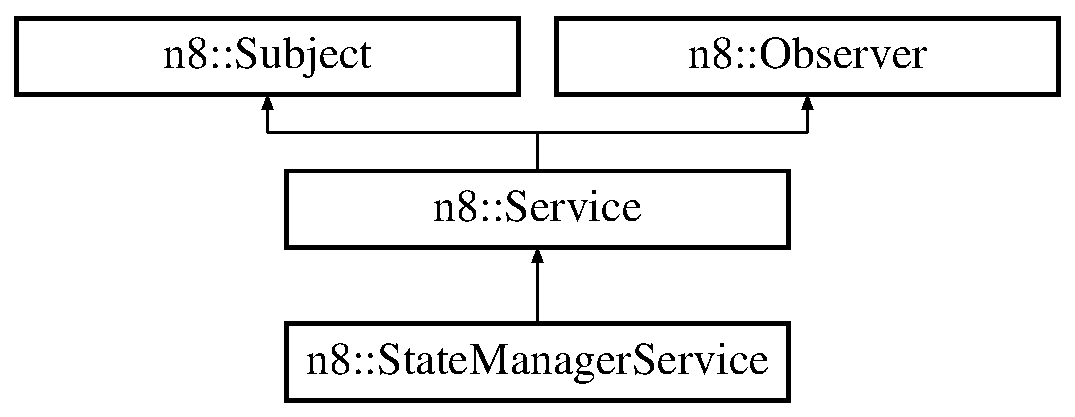
\includegraphics[height=3.000000cm]{classn8_1_1_state_manager_service}
\end{center}
\end{figure}
\subsection*{Public Member Functions}
\begin{DoxyCompactItemize}
\item 
\hyperlink{classn8_1_1_state_manager_service_af22d4c68cce45903992e1bfcb12e85f3}{State\-Manager\-Service} ()
\item 
\hyperlink{classn8_1_1_state_manager_service_a6293e74d12398884b2154dda87f507ce}{$\sim$\-State\-Manager\-Service} ()
\item 
bool \hyperlink{classn8_1_1_state_manager_service_a287093da3f70c807293f3199aa9a6232}{Register\-State} (\hyperlink{namespace_e_state_aee586325ec9fecd1205d41439870dd81}{E\-State\-::\-Values} identifier, \hyperlink{classn8_1_1_state}{State} $\ast$state)
\item 
bool \hyperlink{classn8_1_1_state_manager_service_a4cec486fa154cc2ded5d5c348bf5f140}{Push\-State} (\hyperlink{namespace_e_state_aee586325ec9fecd1205d41439870dd81}{E\-State\-::\-Values} identifier)
\item 
void \hyperlink{classn8_1_1_state_manager_service_a903f56a680ac411d2ae7f34f4e251c38}{Pop\-State} ()
\item 
int \hyperlink{classn8_1_1_state_manager_service_ac553d556b5c925025252719d4319b3de}{Get\-Stack\-Size} ()
\item 
\hyperlink{class_i_d}{I\-D} \hyperlink{classn8_1_1_state_manager_service_a1e11e7a3f32567f416141f436904025d}{Get\-Current\-State\-Id} ()
\item 
void \hyperlink{classn8_1_1_state_manager_service_a85d24e9b582f01d65e90c33fa36a6764}{Process\-State} (Uint32 time, S\-D\-L\-\_\-\-Window $\ast$screen)
\item 
void \hyperlink{classn8_1_1_state_manager_service_a931551f9b6dc470297e9d86abf27b603}{On\-Notify} (\hyperlink{classn8_1_1_event}{Event} $\ast$)
\end{DoxyCompactItemize}
\subsection*{Private Attributes}
\begin{DoxyCompactItemize}
\item 
map$<$ \hyperlink{namespace_e_state_aee586325ec9fecd1205d41439870dd81}{E\-State\-::\-Values}, \hyperlink{classn8_1_1_state}{State} $\ast$ $>$ \hyperlink{classn8_1_1_state_manager_service_a8bc933661f9accae81f82c6e682068c0}{m\-\_\-registered\-States}
\item 
vector$<$ \hyperlink{classn8_1_1_state}{State} $\ast$ $>$ \hyperlink{classn8_1_1_state_manager_service_a3ab9712018eebbfd3b99e406e9b004c0}{m\-\_\-state\-Stack}
\end{DoxyCompactItemize}


\subsection{Detailed Description}
State\-\_\-\-Manager handles the state stack and holds pointers to each registered game state.

The singleton pattern is used so there is a single state stack and access point to state information. 

\subsection{Constructor \& Destructor Documentation}
\hypertarget{classn8_1_1_state_manager_service_af22d4c68cce45903992e1bfcb12e85f3}{\index{n8\-::\-State\-Manager\-Service@{n8\-::\-State\-Manager\-Service}!State\-Manager\-Service@{State\-Manager\-Service}}
\index{State\-Manager\-Service@{State\-Manager\-Service}!n8::StateManagerService@{n8\-::\-State\-Manager\-Service}}
\subsubsection[{State\-Manager\-Service}]{\setlength{\rightskip}{0pt plus 5cm}n8\-::\-State\-Manager\-Service\-::\-State\-Manager\-Service (
\begin{DoxyParamCaption}
{}
\end{DoxyParamCaption}
)}}\label{classn8_1_1_state_manager_service_af22d4c68cce45903992e1bfcb12e85f3}
\hypertarget{classn8_1_1_state_manager_service_a6293e74d12398884b2154dda87f507ce}{\index{n8\-::\-State\-Manager\-Service@{n8\-::\-State\-Manager\-Service}!$\sim$\-State\-Manager\-Service@{$\sim$\-State\-Manager\-Service}}
\index{$\sim$\-State\-Manager\-Service@{$\sim$\-State\-Manager\-Service}!n8::StateManagerService@{n8\-::\-State\-Manager\-Service}}
\subsubsection[{$\sim$\-State\-Manager\-Service}]{\setlength{\rightskip}{0pt plus 5cm}n8\-::\-State\-Manager\-Service\-::$\sim$\-State\-Manager\-Service (
\begin{DoxyParamCaption}
{}
\end{DoxyParamCaption}
)}}\label{classn8_1_1_state_manager_service_a6293e74d12398884b2154dda87f507ce}
Virtual destructor Deletes registered game states 

\subsection{Member Function Documentation}
\hypertarget{classn8_1_1_state_manager_service_a1e11e7a3f32567f416141f436904025d}{\index{n8\-::\-State\-Manager\-Service@{n8\-::\-State\-Manager\-Service}!Get\-Current\-State\-Id@{Get\-Current\-State\-Id}}
\index{Get\-Current\-State\-Id@{Get\-Current\-State\-Id}!n8::StateManagerService@{n8\-::\-State\-Manager\-Service}}
\subsubsection[{Get\-Current\-State\-Id}]{\setlength{\rightskip}{0pt plus 5cm}{\bf I\-D} n8\-::\-State\-Manager\-Service\-::\-Get\-Current\-State\-Id (
\begin{DoxyParamCaption}
{}
\end{DoxyParamCaption}
)}}\label{classn8_1_1_state_manager_service_a1e11e7a3f32567f416141f436904025d}
Gives access to the identifier of the current state object

\begin{DoxyReturn}{Returns}
The \hyperlink{class_i_d}{I\-D} object of the current state object 
\end{DoxyReturn}
\hypertarget{classn8_1_1_state_manager_service_ac553d556b5c925025252719d4319b3de}{\index{n8\-::\-State\-Manager\-Service@{n8\-::\-State\-Manager\-Service}!Get\-Stack\-Size@{Get\-Stack\-Size}}
\index{Get\-Stack\-Size@{Get\-Stack\-Size}!n8::StateManagerService@{n8\-::\-State\-Manager\-Service}}
\subsubsection[{Get\-Stack\-Size}]{\setlength{\rightskip}{0pt plus 5cm}int n8\-::\-State\-Manager\-Service\-::\-Get\-Stack\-Size (
\begin{DoxyParamCaption}
{}
\end{DoxyParamCaption}
)}}\label{classn8_1_1_state_manager_service_ac553d556b5c925025252719d4319b3de}
Returns the size of the state stack

\begin{DoxyReturn}{Returns}
The integer size of the state stack 
\end{DoxyReturn}
\hypertarget{classn8_1_1_state_manager_service_a931551f9b6dc470297e9d86abf27b603}{\index{n8\-::\-State\-Manager\-Service@{n8\-::\-State\-Manager\-Service}!On\-Notify@{On\-Notify}}
\index{On\-Notify@{On\-Notify}!n8::StateManagerService@{n8\-::\-State\-Manager\-Service}}
\subsubsection[{On\-Notify}]{\setlength{\rightskip}{0pt plus 5cm}void n8\-::\-State\-Manager\-Service\-::\-On\-Notify (
\begin{DoxyParamCaption}
\item[{{\bf n8\-::\-Event} $\ast$}]{event}
\end{DoxyParamCaption}
)\hspace{0.3cm}{\ttfamily [virtual]}}}\label{classn8_1_1_state_manager_service_a931551f9b6dc470297e9d86abf27b603}


Implements \hyperlink{classn8_1_1_service_a756a170eba7e5c34a1c12008e22d3ca7}{n8\-::\-Service}.

\hypertarget{classn8_1_1_state_manager_service_a903f56a680ac411d2ae7f34f4e251c38}{\index{n8\-::\-State\-Manager\-Service@{n8\-::\-State\-Manager\-Service}!Pop\-State@{Pop\-State}}
\index{Pop\-State@{Pop\-State}!n8::StateManagerService@{n8\-::\-State\-Manager\-Service}}
\subsubsection[{Pop\-State}]{\setlength{\rightskip}{0pt plus 5cm}void n8\-::\-State\-Manager\-Service\-::\-Pop\-State (
\begin{DoxyParamCaption}
{}
\end{DoxyParamCaption}
)}}\label{classn8_1_1_state_manager_service_a903f56a680ac411d2ae7f34f4e251c38}
If the state stack isn't empty, the top state is popped off \hypertarget{classn8_1_1_state_manager_service_a85d24e9b582f01d65e90c33fa36a6764}{\index{n8\-::\-State\-Manager\-Service@{n8\-::\-State\-Manager\-Service}!Process\-State@{Process\-State}}
\index{Process\-State@{Process\-State}!n8::StateManagerService@{n8\-::\-State\-Manager\-Service}}
\subsubsection[{Process\-State}]{\setlength{\rightskip}{0pt plus 5cm}void n8\-::\-State\-Manager\-Service\-::\-Process\-State (
\begin{DoxyParamCaption}
\item[{Uint32}]{time, }
\item[{S\-D\-L\-\_\-\-Window $\ast$}]{screen}
\end{DoxyParamCaption}
)}}\label{classn8_1_1_state_manager_service_a85d24e9b582f01d65e90c33fa36a6764}
Processes a state by handling input events, updating the state logic, and rendering the state


\begin{DoxyParams}{Parameters}
{\em time} & The current system time \\
\hline
{\em screen} & The screen canvas for rendering \\
\hline
\end{DoxyParams}
\hypertarget{classn8_1_1_state_manager_service_a4cec486fa154cc2ded5d5c348bf5f140}{\index{n8\-::\-State\-Manager\-Service@{n8\-::\-State\-Manager\-Service}!Push\-State@{Push\-State}}
\index{Push\-State@{Push\-State}!n8::StateManagerService@{n8\-::\-State\-Manager\-Service}}
\subsubsection[{Push\-State}]{\setlength{\rightskip}{0pt plus 5cm}bool n8\-::\-State\-Manager\-Service\-::\-Push\-State (
\begin{DoxyParamCaption}
\item[{{\bf E\-State\-::\-Values}}]{identifier}
\end{DoxyParamCaption}
)}}\label{classn8_1_1_state_manager_service_a4cec486fa154cc2ded5d5c348bf5f140}
Pushes a new \hyperlink{classn8_1_1_state}{State} pointer onto the state stack. If the identifier hasn't been registered with the system nothing is pushed onto the stack.


\begin{DoxyParams}{Parameters}
{\em identifier} & The map key for a stored \hyperlink{classn8_1_1_state}{State} pointer\\
\hline
\end{DoxyParams}
\begin{DoxyReturn}{Returns}
True if a \hyperlink{classn8_1_1_state}{State} was pushed onto the stack, false otherwise. 
\end{DoxyReturn}
\hypertarget{classn8_1_1_state_manager_service_a287093da3f70c807293f3199aa9a6232}{\index{n8\-::\-State\-Manager\-Service@{n8\-::\-State\-Manager\-Service}!Register\-State@{Register\-State}}
\index{Register\-State@{Register\-State}!n8::StateManagerService@{n8\-::\-State\-Manager\-Service}}
\subsubsection[{Register\-State}]{\setlength{\rightskip}{0pt plus 5cm}bool n8\-::\-State\-Manager\-Service\-::\-Register\-State (
\begin{DoxyParamCaption}
\item[{{\bf E\-State\-::\-Values}}]{identifier, }
\item[{{\bf State} $\ast$}]{state}
\end{DoxyParamCaption}
)}}\label{classn8_1_1_state_manager_service_a287093da3f70c807293f3199aa9a6232}
Stores a pointer to a \hyperlink{classn8_1_1_state}{State} subclass in a map. If there are no states currently in the state stack, the state being added is pushed onto the stack. If a state with the specified identifier has previously been added, the new state is not added to the map.


\begin{DoxyParams}{Parameters}
{\em identifier} & An integer identifier for the state. Used to differentiate states and to change states. \\
\hline
{\em state} & A pointer to a \hyperlink{classn8_1_1_state}{State} subcalss object\\
\hline
\end{DoxyParams}
\begin{DoxyReturn}{Returns}
True if the state was succesffuly stored in the map; False otherwise. 
\end{DoxyReturn}


\subsection{Member Data Documentation}
\hypertarget{classn8_1_1_state_manager_service_a8bc933661f9accae81f82c6e682068c0}{\index{n8\-::\-State\-Manager\-Service@{n8\-::\-State\-Manager\-Service}!m\-\_\-registered\-States@{m\-\_\-registered\-States}}
\index{m\-\_\-registered\-States@{m\-\_\-registered\-States}!n8::StateManagerService@{n8\-::\-State\-Manager\-Service}}
\subsubsection[{m\-\_\-registered\-States}]{\setlength{\rightskip}{0pt plus 5cm}map$<${\bf E\-State\-::\-Values}, {\bf State}$\ast$$>$ n8\-::\-State\-Manager\-Service\-::m\-\_\-registered\-States\hspace{0.3cm}{\ttfamily [private]}}}\label{classn8_1_1_state_manager_service_a8bc933661f9accae81f82c6e682068c0}
\hypertarget{classn8_1_1_state_manager_service_a3ab9712018eebbfd3b99e406e9b004c0}{\index{n8\-::\-State\-Manager\-Service@{n8\-::\-State\-Manager\-Service}!m\-\_\-state\-Stack@{m\-\_\-state\-Stack}}
\index{m\-\_\-state\-Stack@{m\-\_\-state\-Stack}!n8::StateManagerService@{n8\-::\-State\-Manager\-Service}}
\subsubsection[{m\-\_\-state\-Stack}]{\setlength{\rightskip}{0pt plus 5cm}vector$<${\bf State}$\ast$$>$ n8\-::\-State\-Manager\-Service\-::m\-\_\-state\-Stack\hspace{0.3cm}{\ttfamily [private]}}}\label{classn8_1_1_state_manager_service_a3ab9712018eebbfd3b99e406e9b004c0}
$<$ map of identifiers and game state objects 

The documentation for this class was generated from the following files\-:\begin{DoxyCompactItemize}
\item 
Services/\hyperlink{_state_manager_service_8h}{State\-Manager\-Service.\-h}\item 
Services/\hyperlink{_state_manager_service_8cpp}{State\-Manager\-Service.\-cpp}\end{DoxyCompactItemize}

\hypertarget{classtinyxml2_1_1_str_pair}{\section{tinyxml2\-:\-:Str\-Pair Class Reference}
\label{classtinyxml2_1_1_str_pair}\index{tinyxml2\-::\-Str\-Pair@{tinyxml2\-::\-Str\-Pair}}
}


{\ttfamily \#include $<$tinyxml2.\-h$>$}

\subsection*{Public Types}
\begin{DoxyCompactItemize}
\item 
enum \{ \\*
\hyperlink{classtinyxml2_1_1_str_pair_a0301ef962e15dd94574431f1c61266c5a4f1e01a55f8efe4ca72c32d454060237}{N\-E\-E\-D\-S\-\_\-\-E\-N\-T\-I\-T\-Y\-\_\-\-P\-R\-O\-C\-E\-S\-S\-I\-N\-G} = 0x01, 
\hyperlink{classtinyxml2_1_1_str_pair_a0301ef962e15dd94574431f1c61266c5a8f2045d56e70745d718672c0da91d0e0}{N\-E\-E\-D\-S\-\_\-\-N\-E\-W\-L\-I\-N\-E\-\_\-\-N\-O\-R\-M\-A\-L\-I\-Z\-A\-T\-I\-O\-N} = 0x02, 
\hyperlink{classtinyxml2_1_1_str_pair_a0301ef962e15dd94574431f1c61266c5ab17a85f396c221811fe49263bf6f843f}{C\-O\-L\-L\-A\-P\-S\-E\-\_\-\-W\-H\-I\-T\-E\-S\-P\-A\-C\-E} = 0x04, 
\hyperlink{classtinyxml2_1_1_str_pair_a0301ef962e15dd94574431f1c61266c5aae519eb5a639858591763aa5fc6cc953}{T\-E\-X\-T\-\_\-\-E\-L\-E\-M\-E\-N\-T} = N\-E\-E\-D\-S\-\_\-\-E\-N\-T\-I\-T\-Y\-\_\-\-P\-R\-O\-C\-E\-S\-S\-I\-N\-G $|$ N\-E\-E\-D\-S\-\_\-\-N\-E\-W\-L\-I\-N\-E\-\_\-\-N\-O\-R\-M\-A\-L\-I\-Z\-A\-T\-I\-O\-N, 
\\*
\hyperlink{classtinyxml2_1_1_str_pair_a0301ef962e15dd94574431f1c61266c5a96be48cf899bfeea0aa227f984f1fa63}{T\-E\-X\-T\-\_\-\-E\-L\-E\-M\-E\-N\-T\-\_\-\-L\-E\-A\-V\-E\-\_\-\-E\-N\-T\-I\-T\-I\-E\-S} = N\-E\-E\-D\-S\-\_\-\-N\-E\-W\-L\-I\-N\-E\-\_\-\-N\-O\-R\-M\-A\-L\-I\-Z\-A\-T\-I\-O\-N, 
\hyperlink{classtinyxml2_1_1_str_pair_a0301ef962e15dd94574431f1c61266c5aaab1cbefaa977e6f772b4e2575417aeb}{A\-T\-T\-R\-I\-B\-U\-T\-E\-\_\-\-N\-A\-M\-E} = 0, 
\hyperlink{classtinyxml2_1_1_str_pair_a0301ef962e15dd94574431f1c61266c5a6d72f9ce15f50e8bcd680edf66235dfd}{A\-T\-T\-R\-I\-B\-U\-T\-E\-\_\-\-V\-A\-L\-U\-E} = N\-E\-E\-D\-S\-\_\-\-E\-N\-T\-I\-T\-Y\-\_\-\-P\-R\-O\-C\-E\-S\-S\-I\-N\-G $|$ N\-E\-E\-D\-S\-\_\-\-N\-E\-W\-L\-I\-N\-E\-\_\-\-N\-O\-R\-M\-A\-L\-I\-Z\-A\-T\-I\-O\-N, 
\hyperlink{classtinyxml2_1_1_str_pair_a0301ef962e15dd94574431f1c61266c5a2decbd2513ac14f8befa987938326399}{A\-T\-T\-R\-I\-B\-U\-T\-E\-\_\-\-V\-A\-L\-U\-E\-\_\-\-L\-E\-A\-V\-E\-\_\-\-E\-N\-T\-I\-T\-I\-E\-S} = N\-E\-E\-D\-S\-\_\-\-N\-E\-W\-L\-I\-N\-E\-\_\-\-N\-O\-R\-M\-A\-L\-I\-Z\-A\-T\-I\-O\-N, 
\\*
\hyperlink{classtinyxml2_1_1_str_pair_a0301ef962e15dd94574431f1c61266c5a067a6ec90c8beea1cf5992930d93bffa}{C\-O\-M\-M\-E\-N\-T} = N\-E\-E\-D\-S\-\_\-\-N\-E\-W\-L\-I\-N\-E\-\_\-\-N\-O\-R\-M\-A\-L\-I\-Z\-A\-T\-I\-O\-N
 \}
\end{DoxyCompactItemize}
\subsection*{Public Member Functions}
\begin{DoxyCompactItemize}
\item 
\hyperlink{classtinyxml2_1_1_str_pair_a69153963f7052de9f767d3d8c1623a70}{Str\-Pair} ()
\item 
\hyperlink{classtinyxml2_1_1_str_pair_a60bed84d2503296e1c2a73fcef1431f9}{$\sim$\-Str\-Pair} ()
\item 
void \hyperlink{classtinyxml2_1_1_str_pair_a4f05549373394266a1eecba26813c166}{Set} (char $\ast$start, char $\ast$end, int flags)
\item 
const char $\ast$ \hyperlink{classtinyxml2_1_1_str_pair_ad87e3d11330f5e689ba1e7e54c023b57}{Get\-Str} ()
\item 
bool \hyperlink{classtinyxml2_1_1_str_pair_affa1043e73a18f05d5d2faec055725a7}{Empty} () const 
\item 
void \hyperlink{classtinyxml2_1_1_str_pair_a2baf6230e18333e02ab65d0897ee3941}{Set\-Interned\-Str} (const char $\ast$str)
\item 
void \hyperlink{classtinyxml2_1_1_str_pair_a1f82ec6b5bee35ee7466d8565e43b1de}{Set\-Str} (const char $\ast$str, int flags=0)
\item 
char $\ast$ \hyperlink{classtinyxml2_1_1_str_pair_ad90521f188e9606a8fbafe5d86fb2246}{Parse\-Text} (char $\ast$in, const char $\ast$end\-Tag, int str\-Flags)
\item 
char $\ast$ \hyperlink{classtinyxml2_1_1_str_pair_aa6d8998efceba41d87ec2300c70a6085}{Parse\-Name} (char $\ast$in)
\end{DoxyCompactItemize}
\subsection*{Private Types}
\begin{DoxyCompactItemize}
\item 
enum \{ \hyperlink{classtinyxml2_1_1_str_pair_a476a92d76f24486c3ae4731916b12aaea2d8841daedc3955ed20ec9f760318434}{N\-E\-E\-D\-S\-\_\-\-F\-L\-U\-S\-H} = 0x100, 
\hyperlink{classtinyxml2_1_1_str_pair_a476a92d76f24486c3ae4731916b12aaeab9a3152ce5df9e7f4bbf3774fe862c75}{N\-E\-E\-D\-S\-\_\-\-D\-E\-L\-E\-T\-E} = 0x200
 \}
\end{DoxyCompactItemize}
\subsection*{Private Member Functions}
\begin{DoxyCompactItemize}
\item 
void \hyperlink{classtinyxml2_1_1_str_pair_a80c1b3bd99bf62ae85c94a29ce537125}{Reset} ()
\item 
void \hyperlink{classtinyxml2_1_1_str_pair_ade1469025e6b4cac74397a82a7429337}{Collapse\-Whitespace} ()
\end{DoxyCompactItemize}
\subsection*{Private Attributes}
\begin{DoxyCompactItemize}
\item 
int \hyperlink{classtinyxml2_1_1_str_pair_ae6fabc08e7b24b0d41fa5f2fadbda4ed}{\-\_\-flags}
\item 
char $\ast$ \hyperlink{classtinyxml2_1_1_str_pair_acfd8687916a02833cc55c279460d2f4a}{\-\_\-start}
\item 
char $\ast$ \hyperlink{classtinyxml2_1_1_str_pair_a855c81f785458d8f84313221f2d4a1eb}{\-\_\-end}
\end{DoxyCompactItemize}


\subsection{Member Enumeration Documentation}
\hypertarget{classtinyxml2_1_1_str_pair_a0301ef962e15dd94574431f1c61266c5}{\subsubsection[{anonymous enum}]{\setlength{\rightskip}{0pt plus 5cm}anonymous enum}}\label{classtinyxml2_1_1_str_pair_a0301ef962e15dd94574431f1c61266c5}
\begin{Desc}
\item[Enumerator]\par
\begin{description}
\index{N\-E\-E\-D\-S\-\_\-\-E\-N\-T\-I\-T\-Y\-\_\-\-P\-R\-O\-C\-E\-S\-S\-I\-N\-G@{N\-E\-E\-D\-S\-\_\-\-E\-N\-T\-I\-T\-Y\-\_\-\-P\-R\-O\-C\-E\-S\-S\-I\-N\-G}!tinyxml2\-::\-Str\-Pair@{tinyxml2\-::\-Str\-Pair}}\index{tinyxml2\-::\-Str\-Pair@{tinyxml2\-::\-Str\-Pair}!N\-E\-E\-D\-S\-\_\-\-E\-N\-T\-I\-T\-Y\-\_\-\-P\-R\-O\-C\-E\-S\-S\-I\-N\-G@{N\-E\-E\-D\-S\-\_\-\-E\-N\-T\-I\-T\-Y\-\_\-\-P\-R\-O\-C\-E\-S\-S\-I\-N\-G}}\item[{\em 
\hypertarget{classtinyxml2_1_1_str_pair_a0301ef962e15dd94574431f1c61266c5a4f1e01a55f8efe4ca72c32d454060237}{N\-E\-E\-D\-S\-\_\-\-E\-N\-T\-I\-T\-Y\-\_\-\-P\-R\-O\-C\-E\-S\-S\-I\-N\-G}\label{classtinyxml2_1_1_str_pair_a0301ef962e15dd94574431f1c61266c5a4f1e01a55f8efe4ca72c32d454060237}
}]\index{N\-E\-E\-D\-S\-\_\-\-N\-E\-W\-L\-I\-N\-E\-\_\-\-N\-O\-R\-M\-A\-L\-I\-Z\-A\-T\-I\-O\-N@{N\-E\-E\-D\-S\-\_\-\-N\-E\-W\-L\-I\-N\-E\-\_\-\-N\-O\-R\-M\-A\-L\-I\-Z\-A\-T\-I\-O\-N}!tinyxml2\-::\-Str\-Pair@{tinyxml2\-::\-Str\-Pair}}\index{tinyxml2\-::\-Str\-Pair@{tinyxml2\-::\-Str\-Pair}!N\-E\-E\-D\-S\-\_\-\-N\-E\-W\-L\-I\-N\-E\-\_\-\-N\-O\-R\-M\-A\-L\-I\-Z\-A\-T\-I\-O\-N@{N\-E\-E\-D\-S\-\_\-\-N\-E\-W\-L\-I\-N\-E\-\_\-\-N\-O\-R\-M\-A\-L\-I\-Z\-A\-T\-I\-O\-N}}\item[{\em 
\hypertarget{classtinyxml2_1_1_str_pair_a0301ef962e15dd94574431f1c61266c5a8f2045d56e70745d718672c0da91d0e0}{N\-E\-E\-D\-S\-\_\-\-N\-E\-W\-L\-I\-N\-E\-\_\-\-N\-O\-R\-M\-A\-L\-I\-Z\-A\-T\-I\-O\-N}\label{classtinyxml2_1_1_str_pair_a0301ef962e15dd94574431f1c61266c5a8f2045d56e70745d718672c0da91d0e0}
}]\index{C\-O\-L\-L\-A\-P\-S\-E\-\_\-\-W\-H\-I\-T\-E\-S\-P\-A\-C\-E@{C\-O\-L\-L\-A\-P\-S\-E\-\_\-\-W\-H\-I\-T\-E\-S\-P\-A\-C\-E}!tinyxml2\-::\-Str\-Pair@{tinyxml2\-::\-Str\-Pair}}\index{tinyxml2\-::\-Str\-Pair@{tinyxml2\-::\-Str\-Pair}!C\-O\-L\-L\-A\-P\-S\-E\-\_\-\-W\-H\-I\-T\-E\-S\-P\-A\-C\-E@{C\-O\-L\-L\-A\-P\-S\-E\-\_\-\-W\-H\-I\-T\-E\-S\-P\-A\-C\-E}}\item[{\em 
\hypertarget{classtinyxml2_1_1_str_pair_a0301ef962e15dd94574431f1c61266c5ab17a85f396c221811fe49263bf6f843f}{C\-O\-L\-L\-A\-P\-S\-E\-\_\-\-W\-H\-I\-T\-E\-S\-P\-A\-C\-E}\label{classtinyxml2_1_1_str_pair_a0301ef962e15dd94574431f1c61266c5ab17a85f396c221811fe49263bf6f843f}
}]\index{T\-E\-X\-T\-\_\-\-E\-L\-E\-M\-E\-N\-T@{T\-E\-X\-T\-\_\-\-E\-L\-E\-M\-E\-N\-T}!tinyxml2\-::\-Str\-Pair@{tinyxml2\-::\-Str\-Pair}}\index{tinyxml2\-::\-Str\-Pair@{tinyxml2\-::\-Str\-Pair}!T\-E\-X\-T\-\_\-\-E\-L\-E\-M\-E\-N\-T@{T\-E\-X\-T\-\_\-\-E\-L\-E\-M\-E\-N\-T}}\item[{\em 
\hypertarget{classtinyxml2_1_1_str_pair_a0301ef962e15dd94574431f1c61266c5aae519eb5a639858591763aa5fc6cc953}{T\-E\-X\-T\-\_\-\-E\-L\-E\-M\-E\-N\-T}\label{classtinyxml2_1_1_str_pair_a0301ef962e15dd94574431f1c61266c5aae519eb5a639858591763aa5fc6cc953}
}]\index{T\-E\-X\-T\-\_\-\-E\-L\-E\-M\-E\-N\-T\-\_\-\-L\-E\-A\-V\-E\-\_\-\-E\-N\-T\-I\-T\-I\-E\-S@{T\-E\-X\-T\-\_\-\-E\-L\-E\-M\-E\-N\-T\-\_\-\-L\-E\-A\-V\-E\-\_\-\-E\-N\-T\-I\-T\-I\-E\-S}!tinyxml2\-::\-Str\-Pair@{tinyxml2\-::\-Str\-Pair}}\index{tinyxml2\-::\-Str\-Pair@{tinyxml2\-::\-Str\-Pair}!T\-E\-X\-T\-\_\-\-E\-L\-E\-M\-E\-N\-T\-\_\-\-L\-E\-A\-V\-E\-\_\-\-E\-N\-T\-I\-T\-I\-E\-S@{T\-E\-X\-T\-\_\-\-E\-L\-E\-M\-E\-N\-T\-\_\-\-L\-E\-A\-V\-E\-\_\-\-E\-N\-T\-I\-T\-I\-E\-S}}\item[{\em 
\hypertarget{classtinyxml2_1_1_str_pair_a0301ef962e15dd94574431f1c61266c5a96be48cf899bfeea0aa227f984f1fa63}{T\-E\-X\-T\-\_\-\-E\-L\-E\-M\-E\-N\-T\-\_\-\-L\-E\-A\-V\-E\-\_\-\-E\-N\-T\-I\-T\-I\-E\-S}\label{classtinyxml2_1_1_str_pair_a0301ef962e15dd94574431f1c61266c5a96be48cf899bfeea0aa227f984f1fa63}
}]\index{A\-T\-T\-R\-I\-B\-U\-T\-E\-\_\-\-N\-A\-M\-E@{A\-T\-T\-R\-I\-B\-U\-T\-E\-\_\-\-N\-A\-M\-E}!tinyxml2\-::\-Str\-Pair@{tinyxml2\-::\-Str\-Pair}}\index{tinyxml2\-::\-Str\-Pair@{tinyxml2\-::\-Str\-Pair}!A\-T\-T\-R\-I\-B\-U\-T\-E\-\_\-\-N\-A\-M\-E@{A\-T\-T\-R\-I\-B\-U\-T\-E\-\_\-\-N\-A\-M\-E}}\item[{\em 
\hypertarget{classtinyxml2_1_1_str_pair_a0301ef962e15dd94574431f1c61266c5aaab1cbefaa977e6f772b4e2575417aeb}{A\-T\-T\-R\-I\-B\-U\-T\-E\-\_\-\-N\-A\-M\-E}\label{classtinyxml2_1_1_str_pair_a0301ef962e15dd94574431f1c61266c5aaab1cbefaa977e6f772b4e2575417aeb}
}]\index{A\-T\-T\-R\-I\-B\-U\-T\-E\-\_\-\-V\-A\-L\-U\-E@{A\-T\-T\-R\-I\-B\-U\-T\-E\-\_\-\-V\-A\-L\-U\-E}!tinyxml2\-::\-Str\-Pair@{tinyxml2\-::\-Str\-Pair}}\index{tinyxml2\-::\-Str\-Pair@{tinyxml2\-::\-Str\-Pair}!A\-T\-T\-R\-I\-B\-U\-T\-E\-\_\-\-V\-A\-L\-U\-E@{A\-T\-T\-R\-I\-B\-U\-T\-E\-\_\-\-V\-A\-L\-U\-E}}\item[{\em 
\hypertarget{classtinyxml2_1_1_str_pair_a0301ef962e15dd94574431f1c61266c5a6d72f9ce15f50e8bcd680edf66235dfd}{A\-T\-T\-R\-I\-B\-U\-T\-E\-\_\-\-V\-A\-L\-U\-E}\label{classtinyxml2_1_1_str_pair_a0301ef962e15dd94574431f1c61266c5a6d72f9ce15f50e8bcd680edf66235dfd}
}]\index{A\-T\-T\-R\-I\-B\-U\-T\-E\-\_\-\-V\-A\-L\-U\-E\-\_\-\-L\-E\-A\-V\-E\-\_\-\-E\-N\-T\-I\-T\-I\-E\-S@{A\-T\-T\-R\-I\-B\-U\-T\-E\-\_\-\-V\-A\-L\-U\-E\-\_\-\-L\-E\-A\-V\-E\-\_\-\-E\-N\-T\-I\-T\-I\-E\-S}!tinyxml2\-::\-Str\-Pair@{tinyxml2\-::\-Str\-Pair}}\index{tinyxml2\-::\-Str\-Pair@{tinyxml2\-::\-Str\-Pair}!A\-T\-T\-R\-I\-B\-U\-T\-E\-\_\-\-V\-A\-L\-U\-E\-\_\-\-L\-E\-A\-V\-E\-\_\-\-E\-N\-T\-I\-T\-I\-E\-S@{A\-T\-T\-R\-I\-B\-U\-T\-E\-\_\-\-V\-A\-L\-U\-E\-\_\-\-L\-E\-A\-V\-E\-\_\-\-E\-N\-T\-I\-T\-I\-E\-S}}\item[{\em 
\hypertarget{classtinyxml2_1_1_str_pair_a0301ef962e15dd94574431f1c61266c5a2decbd2513ac14f8befa987938326399}{A\-T\-T\-R\-I\-B\-U\-T\-E\-\_\-\-V\-A\-L\-U\-E\-\_\-\-L\-E\-A\-V\-E\-\_\-\-E\-N\-T\-I\-T\-I\-E\-S}\label{classtinyxml2_1_1_str_pair_a0301ef962e15dd94574431f1c61266c5a2decbd2513ac14f8befa987938326399}
}]\index{C\-O\-M\-M\-E\-N\-T@{C\-O\-M\-M\-E\-N\-T}!tinyxml2\-::\-Str\-Pair@{tinyxml2\-::\-Str\-Pair}}\index{tinyxml2\-::\-Str\-Pair@{tinyxml2\-::\-Str\-Pair}!C\-O\-M\-M\-E\-N\-T@{C\-O\-M\-M\-E\-N\-T}}\item[{\em 
\hypertarget{classtinyxml2_1_1_str_pair_a0301ef962e15dd94574431f1c61266c5a067a6ec90c8beea1cf5992930d93bffa}{C\-O\-M\-M\-E\-N\-T}\label{classtinyxml2_1_1_str_pair_a0301ef962e15dd94574431f1c61266c5a067a6ec90c8beea1cf5992930d93bffa}
}]\end{description}
\end{Desc}
\hypertarget{classtinyxml2_1_1_str_pair_a476a92d76f24486c3ae4731916b12aae}{\subsubsection[{anonymous enum}]{\setlength{\rightskip}{0pt plus 5cm}anonymous enum\hspace{0.3cm}{\ttfamily [private]}}}\label{classtinyxml2_1_1_str_pair_a476a92d76f24486c3ae4731916b12aae}
\begin{Desc}
\item[Enumerator]\par
\begin{description}
\index{N\-E\-E\-D\-S\-\_\-\-F\-L\-U\-S\-H@{N\-E\-E\-D\-S\-\_\-\-F\-L\-U\-S\-H}!tinyxml2\-::\-Str\-Pair@{tinyxml2\-::\-Str\-Pair}}\index{tinyxml2\-::\-Str\-Pair@{tinyxml2\-::\-Str\-Pair}!N\-E\-E\-D\-S\-\_\-\-F\-L\-U\-S\-H@{N\-E\-E\-D\-S\-\_\-\-F\-L\-U\-S\-H}}\item[{\em 
\hypertarget{classtinyxml2_1_1_str_pair_a476a92d76f24486c3ae4731916b12aaea2d8841daedc3955ed20ec9f760318434}{N\-E\-E\-D\-S\-\_\-\-F\-L\-U\-S\-H}\label{classtinyxml2_1_1_str_pair_a476a92d76f24486c3ae4731916b12aaea2d8841daedc3955ed20ec9f760318434}
}]\index{N\-E\-E\-D\-S\-\_\-\-D\-E\-L\-E\-T\-E@{N\-E\-E\-D\-S\-\_\-\-D\-E\-L\-E\-T\-E}!tinyxml2\-::\-Str\-Pair@{tinyxml2\-::\-Str\-Pair}}\index{tinyxml2\-::\-Str\-Pair@{tinyxml2\-::\-Str\-Pair}!N\-E\-E\-D\-S\-\_\-\-D\-E\-L\-E\-T\-E@{N\-E\-E\-D\-S\-\_\-\-D\-E\-L\-E\-T\-E}}\item[{\em 
\hypertarget{classtinyxml2_1_1_str_pair_a476a92d76f24486c3ae4731916b12aaeab9a3152ce5df9e7f4bbf3774fe862c75}{N\-E\-E\-D\-S\-\_\-\-D\-E\-L\-E\-T\-E}\label{classtinyxml2_1_1_str_pair_a476a92d76f24486c3ae4731916b12aaeab9a3152ce5df9e7f4bbf3774fe862c75}
}]\end{description}
\end{Desc}


\subsection{Constructor \& Destructor Documentation}
\hypertarget{classtinyxml2_1_1_str_pair_a69153963f7052de9f767d3d8c1623a70}{\index{tinyxml2\-::\-Str\-Pair@{tinyxml2\-::\-Str\-Pair}!Str\-Pair@{Str\-Pair}}
\index{Str\-Pair@{Str\-Pair}!tinyxml2::StrPair@{tinyxml2\-::\-Str\-Pair}}
\subsubsection[{Str\-Pair}]{\setlength{\rightskip}{0pt plus 5cm}tinyxml2\-::\-Str\-Pair\-::\-Str\-Pair (
\begin{DoxyParamCaption}
{}
\end{DoxyParamCaption}
)\hspace{0.3cm}{\ttfamily [inline]}}}\label{classtinyxml2_1_1_str_pair_a69153963f7052de9f767d3d8c1623a70}
\hypertarget{classtinyxml2_1_1_str_pair_a60bed84d2503296e1c2a73fcef1431f9}{\index{tinyxml2\-::\-Str\-Pair@{tinyxml2\-::\-Str\-Pair}!$\sim$\-Str\-Pair@{$\sim$\-Str\-Pair}}
\index{$\sim$\-Str\-Pair@{$\sim$\-Str\-Pair}!tinyxml2::StrPair@{tinyxml2\-::\-Str\-Pair}}
\subsubsection[{$\sim$\-Str\-Pair}]{\setlength{\rightskip}{0pt plus 5cm}tinyxml2\-::\-Str\-Pair\-::$\sim$\-Str\-Pair (
\begin{DoxyParamCaption}
{}
\end{DoxyParamCaption}
)}}\label{classtinyxml2_1_1_str_pair_a60bed84d2503296e1c2a73fcef1431f9}


\subsection{Member Function Documentation}
\hypertarget{classtinyxml2_1_1_str_pair_ade1469025e6b4cac74397a82a7429337}{\index{tinyxml2\-::\-Str\-Pair@{tinyxml2\-::\-Str\-Pair}!Collapse\-Whitespace@{Collapse\-Whitespace}}
\index{Collapse\-Whitespace@{Collapse\-Whitespace}!tinyxml2::StrPair@{tinyxml2\-::\-Str\-Pair}}
\subsubsection[{Collapse\-Whitespace}]{\setlength{\rightskip}{0pt plus 5cm}void tinyxml2\-::\-Str\-Pair\-::\-Collapse\-Whitespace (
\begin{DoxyParamCaption}
{}
\end{DoxyParamCaption}
)\hspace{0.3cm}{\ttfamily [private]}}}\label{classtinyxml2_1_1_str_pair_ade1469025e6b4cac74397a82a7429337}
\hypertarget{classtinyxml2_1_1_str_pair_affa1043e73a18f05d5d2faec055725a7}{\index{tinyxml2\-::\-Str\-Pair@{tinyxml2\-::\-Str\-Pair}!Empty@{Empty}}
\index{Empty@{Empty}!tinyxml2::StrPair@{tinyxml2\-::\-Str\-Pair}}
\subsubsection[{Empty}]{\setlength{\rightskip}{0pt plus 5cm}bool tinyxml2\-::\-Str\-Pair\-::\-Empty (
\begin{DoxyParamCaption}
{}
\end{DoxyParamCaption}
) const\hspace{0.3cm}{\ttfamily [inline]}}}\label{classtinyxml2_1_1_str_pair_affa1043e73a18f05d5d2faec055725a7}
\hypertarget{classtinyxml2_1_1_str_pair_ad87e3d11330f5e689ba1e7e54c023b57}{\index{tinyxml2\-::\-Str\-Pair@{tinyxml2\-::\-Str\-Pair}!Get\-Str@{Get\-Str}}
\index{Get\-Str@{Get\-Str}!tinyxml2::StrPair@{tinyxml2\-::\-Str\-Pair}}
\subsubsection[{Get\-Str}]{\setlength{\rightskip}{0pt plus 5cm}const char $\ast$ tinyxml2\-::\-Str\-Pair\-::\-Get\-Str (
\begin{DoxyParamCaption}
{}
\end{DoxyParamCaption}
)}}\label{classtinyxml2_1_1_str_pair_ad87e3d11330f5e689ba1e7e54c023b57}
\hypertarget{classtinyxml2_1_1_str_pair_aa6d8998efceba41d87ec2300c70a6085}{\index{tinyxml2\-::\-Str\-Pair@{tinyxml2\-::\-Str\-Pair}!Parse\-Name@{Parse\-Name}}
\index{Parse\-Name@{Parse\-Name}!tinyxml2::StrPair@{tinyxml2\-::\-Str\-Pair}}
\subsubsection[{Parse\-Name}]{\setlength{\rightskip}{0pt plus 5cm}char $\ast$ tinyxml2\-::\-Str\-Pair\-::\-Parse\-Name (
\begin{DoxyParamCaption}
\item[{char $\ast$}]{in}
\end{DoxyParamCaption}
)}}\label{classtinyxml2_1_1_str_pair_aa6d8998efceba41d87ec2300c70a6085}
\hypertarget{classtinyxml2_1_1_str_pair_ad90521f188e9606a8fbafe5d86fb2246}{\index{tinyxml2\-::\-Str\-Pair@{tinyxml2\-::\-Str\-Pair}!Parse\-Text@{Parse\-Text}}
\index{Parse\-Text@{Parse\-Text}!tinyxml2::StrPair@{tinyxml2\-::\-Str\-Pair}}
\subsubsection[{Parse\-Text}]{\setlength{\rightskip}{0pt plus 5cm}char $\ast$ tinyxml2\-::\-Str\-Pair\-::\-Parse\-Text (
\begin{DoxyParamCaption}
\item[{char $\ast$}]{in, }
\item[{const char $\ast$}]{end\-Tag, }
\item[{int}]{str\-Flags}
\end{DoxyParamCaption}
)}}\label{classtinyxml2_1_1_str_pair_ad90521f188e9606a8fbafe5d86fb2246}
\hypertarget{classtinyxml2_1_1_str_pair_a80c1b3bd99bf62ae85c94a29ce537125}{\index{tinyxml2\-::\-Str\-Pair@{tinyxml2\-::\-Str\-Pair}!Reset@{Reset}}
\index{Reset@{Reset}!tinyxml2::StrPair@{tinyxml2\-::\-Str\-Pair}}
\subsubsection[{Reset}]{\setlength{\rightskip}{0pt plus 5cm}void tinyxml2\-::\-Str\-Pair\-::\-Reset (
\begin{DoxyParamCaption}
{}
\end{DoxyParamCaption}
)\hspace{0.3cm}{\ttfamily [private]}}}\label{classtinyxml2_1_1_str_pair_a80c1b3bd99bf62ae85c94a29ce537125}
\hypertarget{classtinyxml2_1_1_str_pair_a4f05549373394266a1eecba26813c166}{\index{tinyxml2\-::\-Str\-Pair@{tinyxml2\-::\-Str\-Pair}!Set@{Set}}
\index{Set@{Set}!tinyxml2::StrPair@{tinyxml2\-::\-Str\-Pair}}
\subsubsection[{Set}]{\setlength{\rightskip}{0pt plus 5cm}void tinyxml2\-::\-Str\-Pair\-::\-Set (
\begin{DoxyParamCaption}
\item[{char $\ast$}]{start, }
\item[{char $\ast$}]{end, }
\item[{int}]{flags}
\end{DoxyParamCaption}
)\hspace{0.3cm}{\ttfamily [inline]}}}\label{classtinyxml2_1_1_str_pair_a4f05549373394266a1eecba26813c166}
\hypertarget{classtinyxml2_1_1_str_pair_a2baf6230e18333e02ab65d0897ee3941}{\index{tinyxml2\-::\-Str\-Pair@{tinyxml2\-::\-Str\-Pair}!Set\-Interned\-Str@{Set\-Interned\-Str}}
\index{Set\-Interned\-Str@{Set\-Interned\-Str}!tinyxml2::StrPair@{tinyxml2\-::\-Str\-Pair}}
\subsubsection[{Set\-Interned\-Str}]{\setlength{\rightskip}{0pt plus 5cm}void tinyxml2\-::\-Str\-Pair\-::\-Set\-Interned\-Str (
\begin{DoxyParamCaption}
\item[{const char $\ast$}]{str}
\end{DoxyParamCaption}
)\hspace{0.3cm}{\ttfamily [inline]}}}\label{classtinyxml2_1_1_str_pair_a2baf6230e18333e02ab65d0897ee3941}
\hypertarget{classtinyxml2_1_1_str_pair_a1f82ec6b5bee35ee7466d8565e43b1de}{\index{tinyxml2\-::\-Str\-Pair@{tinyxml2\-::\-Str\-Pair}!Set\-Str@{Set\-Str}}
\index{Set\-Str@{Set\-Str}!tinyxml2::StrPair@{tinyxml2\-::\-Str\-Pair}}
\subsubsection[{Set\-Str}]{\setlength{\rightskip}{0pt plus 5cm}void tinyxml2\-::\-Str\-Pair\-::\-Set\-Str (
\begin{DoxyParamCaption}
\item[{const char $\ast$}]{str, }
\item[{int}]{flags = {\ttfamily 0}}
\end{DoxyParamCaption}
)}}\label{classtinyxml2_1_1_str_pair_a1f82ec6b5bee35ee7466d8565e43b1de}


\subsection{Member Data Documentation}
\hypertarget{classtinyxml2_1_1_str_pair_a855c81f785458d8f84313221f2d4a1eb}{\index{tinyxml2\-::\-Str\-Pair@{tinyxml2\-::\-Str\-Pair}!\-\_\-end@{\-\_\-end}}
\index{\-\_\-end@{\-\_\-end}!tinyxml2::StrPair@{tinyxml2\-::\-Str\-Pair}}
\subsubsection[{\-\_\-end}]{\setlength{\rightskip}{0pt plus 5cm}char$\ast$ tinyxml2\-::\-Str\-Pair\-::\-\_\-end\hspace{0.3cm}{\ttfamily [private]}}}\label{classtinyxml2_1_1_str_pair_a855c81f785458d8f84313221f2d4a1eb}
\hypertarget{classtinyxml2_1_1_str_pair_ae6fabc08e7b24b0d41fa5f2fadbda4ed}{\index{tinyxml2\-::\-Str\-Pair@{tinyxml2\-::\-Str\-Pair}!\-\_\-flags@{\-\_\-flags}}
\index{\-\_\-flags@{\-\_\-flags}!tinyxml2::StrPair@{tinyxml2\-::\-Str\-Pair}}
\subsubsection[{\-\_\-flags}]{\setlength{\rightskip}{0pt plus 5cm}int tinyxml2\-::\-Str\-Pair\-::\-\_\-flags\hspace{0.3cm}{\ttfamily [private]}}}\label{classtinyxml2_1_1_str_pair_ae6fabc08e7b24b0d41fa5f2fadbda4ed}
\hypertarget{classtinyxml2_1_1_str_pair_acfd8687916a02833cc55c279460d2f4a}{\index{tinyxml2\-::\-Str\-Pair@{tinyxml2\-::\-Str\-Pair}!\-\_\-start@{\-\_\-start}}
\index{\-\_\-start@{\-\_\-start}!tinyxml2::StrPair@{tinyxml2\-::\-Str\-Pair}}
\subsubsection[{\-\_\-start}]{\setlength{\rightskip}{0pt plus 5cm}char$\ast$ tinyxml2\-::\-Str\-Pair\-::\-\_\-start\hspace{0.3cm}{\ttfamily [private]}}}\label{classtinyxml2_1_1_str_pair_acfd8687916a02833cc55c279460d2f4a}


The documentation for this class was generated from the following files\-:\begin{DoxyCompactItemize}
\item 
Utils/\-X\-M\-L\-\_\-\-Config/\hyperlink{tinyxml2_8h}{tinyxml2.\-h}\item 
Utils/\-X\-M\-L\-\_\-\-Config/\hyperlink{tinyxml2_8cpp}{tinyxml2.\-cpp}\end{DoxyCompactItemize}

\hypertarget{classn8_1_1_subject}{\section{n8\-:\-:Subject Class Reference}
\label{classn8_1_1_subject}\index{n8\-::\-Subject@{n8\-::\-Subject}}
}


{\ttfamily \#include $<$Subject.\-h$>$}

Inheritance diagram for n8\-:\-:Subject\-:\begin{figure}[H]
\begin{center}
\leavevmode
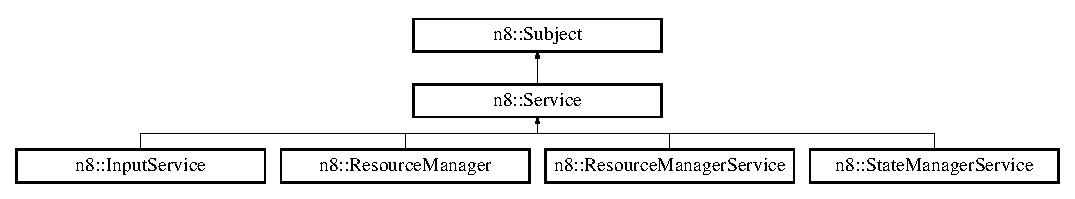
\includegraphics[height=2.222222cm]{classn8_1_1_subject}
\end{center}
\end{figure}
\subsection*{Public Member Functions}
\begin{DoxyCompactItemize}
\item 
void \hyperlink{classn8_1_1_subject_ae12efefe6756166c1521b06db8f633ff}{Add\-Observer} (\hyperlink{classn8_1_1_observer}{Observer} $\ast$observer)
\item 
void \hyperlink{classn8_1_1_subject_a652c26127339aeaf34ccfff6d12ceb64}{Remove\-Observer} (\hyperlink{classn8_1_1_observer}{Observer} $\ast$observer)
\item 
void \hyperlink{classn8_1_1_subject_a74e8ccf2447a062f605ffecefadae2ca}{Notify} (\hyperlink{classn8_1_1_event}{Event} $\ast$)
\end{DoxyCompactItemize}
\subsection*{Private Attributes}
\begin{DoxyCompactItemize}
\item 
std\-::vector$<$ \hyperlink{classn8_1_1_observer}{Observer} $\ast$ $>$ \hyperlink{classn8_1_1_subject_adaf1d665557715d9d22826c59f5fa496}{m\-\_\-observers}
\end{DoxyCompactItemize}


\subsection{Detailed Description}
Subjects inform other systems that an event has occured 

\subsection{Member Function Documentation}
\hypertarget{classn8_1_1_subject_ae12efefe6756166c1521b06db8f633ff}{\index{n8\-::\-Subject@{n8\-::\-Subject}!Add\-Observer@{Add\-Observer}}
\index{Add\-Observer@{Add\-Observer}!n8::Subject@{n8\-::\-Subject}}
\subsubsection[{Add\-Observer}]{\setlength{\rightskip}{0pt plus 5cm}void n8\-::\-Subject\-::\-Add\-Observer (
\begin{DoxyParamCaption}
\item[{{\bf Observer} $\ast$}]{observer}
\end{DoxyParamCaption}
)}}\label{classn8_1_1_subject_ae12efefe6756166c1521b06db8f633ff}
Add\-Observer Adds a pointer to a list of observers to it can be notified of events


\begin{DoxyParams}{Parameters}
{\em observer} & The observer to add to the list \\
\hline
\end{DoxyParams}
\hypertarget{classn8_1_1_subject_a74e8ccf2447a062f605ffecefadae2ca}{\index{n8\-::\-Subject@{n8\-::\-Subject}!Notify@{Notify}}
\index{Notify@{Notify}!n8::Subject@{n8\-::\-Subject}}
\subsubsection[{Notify}]{\setlength{\rightskip}{0pt plus 5cm}void n8\-::\-Subject\-::\-Notify (
\begin{DoxyParamCaption}
\item[{{\bf n8\-::\-Event} $\ast$}]{event}
\end{DoxyParamCaption}
)}}\label{classn8_1_1_subject_a74e8ccf2447a062f605ffecefadae2ca}
Notify Informs observers that some event has occured so they can respond accordingly


\begin{DoxyParams}{Parameters}
{\em event} & The event that has occured and can be handled \\
\hline
\end{DoxyParams}
\hypertarget{classn8_1_1_subject_a652c26127339aeaf34ccfff6d12ceb64}{\index{n8\-::\-Subject@{n8\-::\-Subject}!Remove\-Observer@{Remove\-Observer}}
\index{Remove\-Observer@{Remove\-Observer}!n8::Subject@{n8\-::\-Subject}}
\subsubsection[{Remove\-Observer}]{\setlength{\rightskip}{0pt plus 5cm}void n8\-::\-Subject\-::\-Remove\-Observer (
\begin{DoxyParamCaption}
\item[{{\bf Observer} $\ast$}]{observer}
\end{DoxyParamCaption}
)}}\label{classn8_1_1_subject_a652c26127339aeaf34ccfff6d12ceb64}
Remove\-Observer Removes an observer from the observers list if it is present


\begin{DoxyParams}{Parameters}
{\em observer} & The observer to remove from the observers list \\
\hline
\end{DoxyParams}


\subsection{Member Data Documentation}
\hypertarget{classn8_1_1_subject_adaf1d665557715d9d22826c59f5fa496}{\index{n8\-::\-Subject@{n8\-::\-Subject}!m\-\_\-observers@{m\-\_\-observers}}
\index{m\-\_\-observers@{m\-\_\-observers}!n8::Subject@{n8\-::\-Subject}}
\subsubsection[{m\-\_\-observers}]{\setlength{\rightskip}{0pt plus 5cm}std\-::vector$<${\bf Observer}$\ast$$>$ n8\-::\-Subject\-::m\-\_\-observers\hspace{0.3cm}{\ttfamily [private]}}}\label{classn8_1_1_subject_adaf1d665557715d9d22826c59f5fa496}


The documentation for this class was generated from the following files\-:\begin{DoxyCompactItemize}
\item 
Communication/\hyperlink{_subject_8h}{Subject.\-h}\item 
Communication/\hyperlink{_subject_8cpp}{Subject.\-cpp}\end{DoxyCompactItemize}

\hypertarget{classn8_1_1_timer}{\section{n8\-:\-:Timer Class Reference}
\label{classn8_1_1_timer}\index{n8\-::\-Timer@{n8\-::\-Timer}}
}


{\ttfamily \#include $<$Timer.\-h$>$}

\subsection*{Public Member Functions}
\begin{DoxyCompactItemize}
\item 
\hyperlink{classn8_1_1_timer_ab62468af51fb15209ca5a271060eb908}{Timer} ()
\item 
\hyperlink{classn8_1_1_timer_affebb151acd2dddc3b65ce8420b3029d}{$\sim$\-Timer} ()
\item 
void \hyperlink{classn8_1_1_timer_a00818f30eacc9007a72f6a54b3f1a005}{Update\-Current\-Time} ()
\item 
void \hyperlink{classn8_1_1_timer_a1f13b9e470602c87f38819d7d7e3af5e}{Sync\-Game} (unsigned)
\item 
unsigned int \hyperlink{classn8_1_1_timer_a60c0046328778c542f2b4676d864eabc}{Get\-Elapsed\-Time} ()
\item 
unsigned int \hyperlink{classn8_1_1_timer_aa3e91a189e9c7dc1b54b79a177398638}{Get\-Time} ()
\end{DoxyCompactItemize}
\subsection*{Private Attributes}
\begin{DoxyCompactItemize}
\item 
Uint32 \hyperlink{classn8_1_1_timer_a4ea04e459f66f523e443dad9cfb78241}{m\-\_\-start\-Time}
\item 
Uint32 \hyperlink{classn8_1_1_timer_af8d189a52bfd4dd1d00322602627327d}{m\-\_\-current\-Time}
\end{DoxyCompactItemize}


\subsection{Constructor \& Destructor Documentation}
\hypertarget{classn8_1_1_timer_ab62468af51fb15209ca5a271060eb908}{\index{n8\-::\-Timer@{n8\-::\-Timer}!Timer@{Timer}}
\index{Timer@{Timer}!n8::Timer@{n8\-::\-Timer}}
\subsubsection[{Timer}]{\setlength{\rightskip}{0pt plus 5cm}n8\-::\-Timer\-::\-Timer (
\begin{DoxyParamCaption}
{}
\end{DoxyParamCaption}
)}}\label{classn8_1_1_timer_ab62468af51fb15209ca5a271060eb908}
\hypertarget{classn8_1_1_timer_affebb151acd2dddc3b65ce8420b3029d}{\index{n8\-::\-Timer@{n8\-::\-Timer}!$\sim$\-Timer@{$\sim$\-Timer}}
\index{$\sim$\-Timer@{$\sim$\-Timer}!n8::Timer@{n8\-::\-Timer}}
\subsubsection[{$\sim$\-Timer}]{\setlength{\rightskip}{0pt plus 5cm}n8\-::\-Timer\-::$\sim$\-Timer (
\begin{DoxyParamCaption}
{}
\end{DoxyParamCaption}
)}}\label{classn8_1_1_timer_affebb151acd2dddc3b65ce8420b3029d}


\subsection{Member Function Documentation}
\hypertarget{classn8_1_1_timer_a60c0046328778c542f2b4676d864eabc}{\index{n8\-::\-Timer@{n8\-::\-Timer}!Get\-Elapsed\-Time@{Get\-Elapsed\-Time}}
\index{Get\-Elapsed\-Time@{Get\-Elapsed\-Time}!n8::Timer@{n8\-::\-Timer}}
\subsubsection[{Get\-Elapsed\-Time}]{\setlength{\rightskip}{0pt plus 5cm}unsigned int n8\-::\-Timer\-::\-Get\-Elapsed\-Time (
\begin{DoxyParamCaption}
{}
\end{DoxyParamCaption}
)}}\label{classn8_1_1_timer_a60c0046328778c542f2b4676d864eabc}
\hypertarget{classn8_1_1_timer_aa3e91a189e9c7dc1b54b79a177398638}{\index{n8\-::\-Timer@{n8\-::\-Timer}!Get\-Time@{Get\-Time}}
\index{Get\-Time@{Get\-Time}!n8::Timer@{n8\-::\-Timer}}
\subsubsection[{Get\-Time}]{\setlength{\rightskip}{0pt plus 5cm}unsigned int n8\-::\-Timer\-::\-Get\-Time (
\begin{DoxyParamCaption}
{}
\end{DoxyParamCaption}
)}}\label{classn8_1_1_timer_aa3e91a189e9c7dc1b54b79a177398638}
\hypertarget{classn8_1_1_timer_a1f13b9e470602c87f38819d7d7e3af5e}{\index{n8\-::\-Timer@{n8\-::\-Timer}!Sync\-Game@{Sync\-Game}}
\index{Sync\-Game@{Sync\-Game}!n8::Timer@{n8\-::\-Timer}}
\subsubsection[{Sync\-Game}]{\setlength{\rightskip}{0pt plus 5cm}void n8\-::\-Timer\-::\-Sync\-Game (
\begin{DoxyParamCaption}
\item[{unsigned}]{fps}
\end{DoxyParamCaption}
)}}\label{classn8_1_1_timer_a1f13b9e470602c87f38819d7d7e3af5e}
\hypertarget{classn8_1_1_timer_a00818f30eacc9007a72f6a54b3f1a005}{\index{n8\-::\-Timer@{n8\-::\-Timer}!Update\-Current\-Time@{Update\-Current\-Time}}
\index{Update\-Current\-Time@{Update\-Current\-Time}!n8::Timer@{n8\-::\-Timer}}
\subsubsection[{Update\-Current\-Time}]{\setlength{\rightskip}{0pt plus 5cm}void n8\-::\-Timer\-::\-Update\-Current\-Time (
\begin{DoxyParamCaption}
{}
\end{DoxyParamCaption}
)}}\label{classn8_1_1_timer_a00818f30eacc9007a72f6a54b3f1a005}


\subsection{Member Data Documentation}
\hypertarget{classn8_1_1_timer_af8d189a52bfd4dd1d00322602627327d}{\index{n8\-::\-Timer@{n8\-::\-Timer}!m\-\_\-current\-Time@{m\-\_\-current\-Time}}
\index{m\-\_\-current\-Time@{m\-\_\-current\-Time}!n8::Timer@{n8\-::\-Timer}}
\subsubsection[{m\-\_\-current\-Time}]{\setlength{\rightskip}{0pt plus 5cm}Uint32 n8\-::\-Timer\-::m\-\_\-current\-Time\hspace{0.3cm}{\ttfamily [private]}}}\label{classn8_1_1_timer_af8d189a52bfd4dd1d00322602627327d}
\hypertarget{classn8_1_1_timer_a4ea04e459f66f523e443dad9cfb78241}{\index{n8\-::\-Timer@{n8\-::\-Timer}!m\-\_\-start\-Time@{m\-\_\-start\-Time}}
\index{m\-\_\-start\-Time@{m\-\_\-start\-Time}!n8::Timer@{n8\-::\-Timer}}
\subsubsection[{m\-\_\-start\-Time}]{\setlength{\rightskip}{0pt plus 5cm}Uint32 n8\-::\-Timer\-::m\-\_\-start\-Time\hspace{0.3cm}{\ttfamily [private]}}}\label{classn8_1_1_timer_a4ea04e459f66f523e443dad9cfb78241}


The documentation for this class was generated from the following files\-:\begin{DoxyCompactItemize}
\item 
Core/\hyperlink{_timer_8h}{Timer.\-h}\item 
Core/\hyperlink{_timer_8cpp}{Timer.\-cpp}\end{DoxyCompactItemize}

\hypertarget{classn8_1_1_window}{\section{n8\-:\-:Window Class Reference}
\label{classn8_1_1_window}\index{n8\-::\-Window@{n8\-::\-Window}}
}


{\ttfamily \#include $<$Window.\-h$>$}

\subsection*{Public Member Functions}
\begin{DoxyCompactItemize}
\item 
\hyperlink{classn8_1_1_window_a23d794805d8de4c98efd5ab685349106}{Window} ()
\item 
\hyperlink{classn8_1_1_window_a0e16f0575d10d2182bc9c572b24559ce}{$\sim$\-Window} ()
\item 
void \hyperlink{classn8_1_1_window_aa603ad1f6e4df1327401df37a0e34529}{Set\-Title} (char $\ast$caption)
\item 
void \hyperlink{classn8_1_1_window_ae4ab3029b3ee1eaabe98947738c486f6}{Resize\-Window} (int w, int h)
\item 
S\-D\-L\-\_\-\-Surface $\ast$ \hyperlink{classn8_1_1_window_a1442cc3a052dea262f04cf2c30d868d5}{Get\-Surface} () const 
\item 
S\-D\-L\-\_\-\-Window $\ast$ \hyperlink{classn8_1_1_window_ae218e0dcdc9081e835cb3a136a7e39e5}{Get\-Window} ()
\end{DoxyCompactItemize}
\subsection*{Static Public Attributes}
\begin{DoxyCompactItemize}
\item 
static const int \hyperlink{classn8_1_1_window_ae426fde4ebf20489d6c7d3e37e520f9d}{D\-E\-F\-A\-U\-L\-T\-\_\-\-S\-C\-R\-E\-E\-N\-\_\-\-W\-I\-D\-T\-H} = 400
\item 
static const int \hyperlink{classn8_1_1_window_ac1aa876c38173e9a4fc6e670529424c2}{D\-E\-F\-A\-U\-L\-T\-\_\-\-S\-C\-R\-E\-E\-N\-\_\-\-H\-E\-I\-G\-H\-T} = 400
\item 
static const int \hyperlink{classn8_1_1_window_a2c179aca7c66204e7f9ec7a0d99efdd0}{D\-E\-F\-A\-U\-L\-T\-\_\-\-B\-P\-P} = 32
\end{DoxyCompactItemize}
\subsection*{Private Attributes}
\begin{DoxyCompactItemize}
\item 
unsigned \hyperlink{classn8_1_1_window_acb7bbe7407c00a0f14b5d0a1a42694d8}{m\-\_\-screen\-Width}
\item 
unsigned \hyperlink{classn8_1_1_window_a7a1bc0ad691db2677c94330f743f0915}{m\-\_\-screen\-Height}
\item 
S\-D\-L\-\_\-\-Surface $\ast$ \hyperlink{classn8_1_1_window_a9ba324f2cc04e8183fd9b938dc730222}{m\-\_\-screen\-Surface}
\item 
S\-D\-L\-\_\-\-Window $\ast$ \hyperlink{classn8_1_1_window_ae658f6f3a5aefdde5b699b65fc4337e3}{m\-\_\-window}
\end{DoxyCompactItemize}


\subsection{Constructor \& Destructor Documentation}
\hypertarget{classn8_1_1_window_a23d794805d8de4c98efd5ab685349106}{\index{n8\-::\-Window@{n8\-::\-Window}!Window@{Window}}
\index{Window@{Window}!n8::Window@{n8\-::\-Window}}
\subsubsection[{Window}]{\setlength{\rightskip}{0pt plus 5cm}n8\-::\-Window\-::\-Window (
\begin{DoxyParamCaption}
{}
\end{DoxyParamCaption}
)}}\label{classn8_1_1_window_a23d794805d8de4c98efd5ab685349106}
\hypertarget{classn8_1_1_window_a0e16f0575d10d2182bc9c572b24559ce}{\index{n8\-::\-Window@{n8\-::\-Window}!$\sim$\-Window@{$\sim$\-Window}}
\index{$\sim$\-Window@{$\sim$\-Window}!n8::Window@{n8\-::\-Window}}
\subsubsection[{$\sim$\-Window}]{\setlength{\rightskip}{0pt plus 5cm}n8\-::\-Window\-::$\sim$\-Window (
\begin{DoxyParamCaption}
{}
\end{DoxyParamCaption}
)}}\label{classn8_1_1_window_a0e16f0575d10d2182bc9c572b24559ce}


\subsection{Member Function Documentation}
\hypertarget{classn8_1_1_window_a1442cc3a052dea262f04cf2c30d868d5}{\index{n8\-::\-Window@{n8\-::\-Window}!Get\-Surface@{Get\-Surface}}
\index{Get\-Surface@{Get\-Surface}!n8::Window@{n8\-::\-Window}}
\subsubsection[{Get\-Surface}]{\setlength{\rightskip}{0pt plus 5cm}S\-D\-L\-\_\-\-Surface $\ast$ n8\-::\-Window\-::\-Get\-Surface (
\begin{DoxyParamCaption}
{}
\end{DoxyParamCaption}
) const}}\label{classn8_1_1_window_a1442cc3a052dea262f04cf2c30d868d5}
\begin{DoxyReturn}{Returns}
a pointer to the background surface 
\end{DoxyReturn}
\hypertarget{classn8_1_1_window_ae218e0dcdc9081e835cb3a136a7e39e5}{\index{n8\-::\-Window@{n8\-::\-Window}!Get\-Window@{Get\-Window}}
\index{Get\-Window@{Get\-Window}!n8::Window@{n8\-::\-Window}}
\subsubsection[{Get\-Window}]{\setlength{\rightskip}{0pt plus 5cm}S\-D\-L\-\_\-\-Window $\ast$ n8\-::\-Window\-::\-Get\-Window (
\begin{DoxyParamCaption}
{}
\end{DoxyParamCaption}
)}}\label{classn8_1_1_window_ae218e0dcdc9081e835cb3a136a7e39e5}
\hypertarget{classn8_1_1_window_ae4ab3029b3ee1eaabe98947738c486f6}{\index{n8\-::\-Window@{n8\-::\-Window}!Resize\-Window@{Resize\-Window}}
\index{Resize\-Window@{Resize\-Window}!n8::Window@{n8\-::\-Window}}
\subsubsection[{Resize\-Window}]{\setlength{\rightskip}{0pt plus 5cm}void n8\-::\-Window\-::\-Resize\-Window (
\begin{DoxyParamCaption}
\item[{int}]{w, }
\item[{int}]{h}
\end{DoxyParamCaption}
)}}\label{classn8_1_1_window_ae4ab3029b3ee1eaabe98947738c486f6}
Resizes the screen to the specified dimensions

First the existing screen surface is freed, then a new surface is created with the specified dimensions


\begin{DoxyParams}{Parameters}
{\em w} & The integer width of the screen \\
\hline
{\em h} & The integer height of the screen \\
\hline
{\em bpp} & The bitmap depth \\
\hline
\end{DoxyParams}
\hypertarget{classn8_1_1_window_aa603ad1f6e4df1327401df37a0e34529}{\index{n8\-::\-Window@{n8\-::\-Window}!Set\-Title@{Set\-Title}}
\index{Set\-Title@{Set\-Title}!n8::Window@{n8\-::\-Window}}
\subsubsection[{Set\-Title}]{\setlength{\rightskip}{0pt plus 5cm}void n8\-::\-Window\-::\-Set\-Title (
\begin{DoxyParamCaption}
\item[{char $\ast$}]{caption}
\end{DoxyParamCaption}
)}}\label{classn8_1_1_window_aa603ad1f6e4df1327401df37a0e34529}
Sets the window caption 

\subsection{Member Data Documentation}
\hypertarget{classn8_1_1_window_a2c179aca7c66204e7f9ec7a0d99efdd0}{\index{n8\-::\-Window@{n8\-::\-Window}!D\-E\-F\-A\-U\-L\-T\-\_\-\-B\-P\-P@{D\-E\-F\-A\-U\-L\-T\-\_\-\-B\-P\-P}}
\index{D\-E\-F\-A\-U\-L\-T\-\_\-\-B\-P\-P@{D\-E\-F\-A\-U\-L\-T\-\_\-\-B\-P\-P}!n8::Window@{n8\-::\-Window}}
\subsubsection[{D\-E\-F\-A\-U\-L\-T\-\_\-\-B\-P\-P}]{\setlength{\rightskip}{0pt plus 5cm}const int n8\-::\-Window\-::\-D\-E\-F\-A\-U\-L\-T\-\_\-\-B\-P\-P = 32\hspace{0.3cm}{\ttfamily [static]}}}\label{classn8_1_1_window_a2c179aca7c66204e7f9ec7a0d99efdd0}
\hypertarget{classn8_1_1_window_ac1aa876c38173e9a4fc6e670529424c2}{\index{n8\-::\-Window@{n8\-::\-Window}!D\-E\-F\-A\-U\-L\-T\-\_\-\-S\-C\-R\-E\-E\-N\-\_\-\-H\-E\-I\-G\-H\-T@{D\-E\-F\-A\-U\-L\-T\-\_\-\-S\-C\-R\-E\-E\-N\-\_\-\-H\-E\-I\-G\-H\-T}}
\index{D\-E\-F\-A\-U\-L\-T\-\_\-\-S\-C\-R\-E\-E\-N\-\_\-\-H\-E\-I\-G\-H\-T@{D\-E\-F\-A\-U\-L\-T\-\_\-\-S\-C\-R\-E\-E\-N\-\_\-\-H\-E\-I\-G\-H\-T}!n8::Window@{n8\-::\-Window}}
\subsubsection[{D\-E\-F\-A\-U\-L\-T\-\_\-\-S\-C\-R\-E\-E\-N\-\_\-\-H\-E\-I\-G\-H\-T}]{\setlength{\rightskip}{0pt plus 5cm}const int n8\-::\-Window\-::\-D\-E\-F\-A\-U\-L\-T\-\_\-\-S\-C\-R\-E\-E\-N\-\_\-\-H\-E\-I\-G\-H\-T = 400\hspace{0.3cm}{\ttfamily [static]}}}\label{classn8_1_1_window_ac1aa876c38173e9a4fc6e670529424c2}
\hypertarget{classn8_1_1_window_ae426fde4ebf20489d6c7d3e37e520f9d}{\index{n8\-::\-Window@{n8\-::\-Window}!D\-E\-F\-A\-U\-L\-T\-\_\-\-S\-C\-R\-E\-E\-N\-\_\-\-W\-I\-D\-T\-H@{D\-E\-F\-A\-U\-L\-T\-\_\-\-S\-C\-R\-E\-E\-N\-\_\-\-W\-I\-D\-T\-H}}
\index{D\-E\-F\-A\-U\-L\-T\-\_\-\-S\-C\-R\-E\-E\-N\-\_\-\-W\-I\-D\-T\-H@{D\-E\-F\-A\-U\-L\-T\-\_\-\-S\-C\-R\-E\-E\-N\-\_\-\-W\-I\-D\-T\-H}!n8::Window@{n8\-::\-Window}}
\subsubsection[{D\-E\-F\-A\-U\-L\-T\-\_\-\-S\-C\-R\-E\-E\-N\-\_\-\-W\-I\-D\-T\-H}]{\setlength{\rightskip}{0pt plus 5cm}const int n8\-::\-Window\-::\-D\-E\-F\-A\-U\-L\-T\-\_\-\-S\-C\-R\-E\-E\-N\-\_\-\-W\-I\-D\-T\-H = 400\hspace{0.3cm}{\ttfamily [static]}}}\label{classn8_1_1_window_ae426fde4ebf20489d6c7d3e37e520f9d}
\hypertarget{classn8_1_1_window_a7a1bc0ad691db2677c94330f743f0915}{\index{n8\-::\-Window@{n8\-::\-Window}!m\-\_\-screen\-Height@{m\-\_\-screen\-Height}}
\index{m\-\_\-screen\-Height@{m\-\_\-screen\-Height}!n8::Window@{n8\-::\-Window}}
\subsubsection[{m\-\_\-screen\-Height}]{\setlength{\rightskip}{0pt plus 5cm}unsigned n8\-::\-Window\-::m\-\_\-screen\-Height\hspace{0.3cm}{\ttfamily [private]}}}\label{classn8_1_1_window_a7a1bc0ad691db2677c94330f743f0915}
$<$ width of the screen surface \hypertarget{classn8_1_1_window_a9ba324f2cc04e8183fd9b938dc730222}{\index{n8\-::\-Window@{n8\-::\-Window}!m\-\_\-screen\-Surface@{m\-\_\-screen\-Surface}}
\index{m\-\_\-screen\-Surface@{m\-\_\-screen\-Surface}!n8::Window@{n8\-::\-Window}}
\subsubsection[{m\-\_\-screen\-Surface}]{\setlength{\rightskip}{0pt plus 5cm}S\-D\-L\-\_\-\-Surface$\ast$ n8\-::\-Window\-::m\-\_\-screen\-Surface\hspace{0.3cm}{\ttfamily [private]}}}\label{classn8_1_1_window_a9ba324f2cc04e8183fd9b938dc730222}
$<$ height of the screen surface \hypertarget{classn8_1_1_window_acb7bbe7407c00a0f14b5d0a1a42694d8}{\index{n8\-::\-Window@{n8\-::\-Window}!m\-\_\-screen\-Width@{m\-\_\-screen\-Width}}
\index{m\-\_\-screen\-Width@{m\-\_\-screen\-Width}!n8::Window@{n8\-::\-Window}}
\subsubsection[{m\-\_\-screen\-Width}]{\setlength{\rightskip}{0pt plus 5cm}unsigned n8\-::\-Window\-::m\-\_\-screen\-Width\hspace{0.3cm}{\ttfamily [private]}}}\label{classn8_1_1_window_acb7bbe7407c00a0f14b5d0a1a42694d8}
\hypertarget{classn8_1_1_window_ae658f6f3a5aefdde5b699b65fc4337e3}{\index{n8\-::\-Window@{n8\-::\-Window}!m\-\_\-window@{m\-\_\-window}}
\index{m\-\_\-window@{m\-\_\-window}!n8::Window@{n8\-::\-Window}}
\subsubsection[{m\-\_\-window}]{\setlength{\rightskip}{0pt plus 5cm}S\-D\-L\-\_\-\-Window$\ast$ n8\-::\-Window\-::m\-\_\-window\hspace{0.3cm}{\ttfamily [private]}}}\label{classn8_1_1_window_ae658f6f3a5aefdde5b699b65fc4337e3}
$<$ surface to render things to 

The documentation for this class was generated from the following files\-:\begin{DoxyCompactItemize}
\item 
Core/\hyperlink{_window_8h}{Window.\-h}\item 
Core/\hyperlink{_window_8cpp}{Window.\-cpp}\end{DoxyCompactItemize}

\hypertarget{classtinyxml2_1_1_x_m_l_attribute}{\section{tinyxml2\-:\-:X\-M\-L\-Attribute Class Reference}
\label{classtinyxml2_1_1_x_m_l_attribute}\index{tinyxml2\-::\-X\-M\-L\-Attribute@{tinyxml2\-::\-X\-M\-L\-Attribute}}
}


{\ttfamily \#include $<$tinyxml2.\-h$>$}

\subsection*{Public Member Functions}
\begin{DoxyCompactItemize}
\item 
const char $\ast$ \hyperlink{classtinyxml2_1_1_x_m_l_attribute_a8124fbfd27f57150cc68d8a9207078c3}{Name} () const 
\begin{DoxyCompactList}\small\item\em The name of the attribute. \end{DoxyCompactList}\item 
const char $\ast$ \hyperlink{classtinyxml2_1_1_x_m_l_attribute_aa9b08c6e592b0c88117c46666dcc1af2}{Value} () const 
\begin{DoxyCompactList}\small\item\em The value of the attribute. \end{DoxyCompactList}\item 
const \hyperlink{classtinyxml2_1_1_x_m_l_attribute}{X\-M\-L\-Attribute} $\ast$ \hyperlink{classtinyxml2_1_1_x_m_l_attribute_a7fd852d6185af90361ec1bc9a7681ad6}{Next} () const 
\begin{DoxyCompactList}\small\item\em The next attribute in the list. \end{DoxyCompactList}\item 
int \hyperlink{classtinyxml2_1_1_x_m_l_attribute_a949d02a5888092cc68c1e29185301863}{Int\-Value} () const 
\item 
unsigned \hyperlink{classtinyxml2_1_1_x_m_l_attribute_a4c7a179907836a136d1ce5acbe53389d}{Unsigned\-Value} () const 
\begin{DoxyCompactList}\small\item\em Query as an unsigned integer. See \hyperlink{classtinyxml2_1_1_x_m_l_attribute_a949d02a5888092cc68c1e29185301863}{Int\-Value()} \end{DoxyCompactList}\item 
bool \hyperlink{classtinyxml2_1_1_x_m_l_attribute_afb444b7a12527f836aa161b54b2f7ce7}{Bool\-Value} () const 
\begin{DoxyCompactList}\small\item\em Query as a boolean. See \hyperlink{classtinyxml2_1_1_x_m_l_attribute_a949d02a5888092cc68c1e29185301863}{Int\-Value()} \end{DoxyCompactList}\item 
double \hyperlink{classtinyxml2_1_1_x_m_l_attribute_a336153e5aa1b7ccd6502fc249bfb3fd7}{Double\-Value} () const 
\begin{DoxyCompactList}\small\item\em Query as a double. See \hyperlink{classtinyxml2_1_1_x_m_l_attribute_a949d02a5888092cc68c1e29185301863}{Int\-Value()} \end{DoxyCompactList}\item 
float \hyperlink{classtinyxml2_1_1_x_m_l_attribute_ae3d51ff98eacc1dc46efcfdaee5c84ad}{Float\-Value} () const 
\begin{DoxyCompactList}\small\item\em Query as a float. See \hyperlink{classtinyxml2_1_1_x_m_l_attribute_a949d02a5888092cc68c1e29185301863}{Int\-Value()} \end{DoxyCompactList}\item 
\hyperlink{namespacetinyxml2_a1fbf88509c3ac88c09117b1947414e08}{X\-M\-L\-Error} \hyperlink{classtinyxml2_1_1_x_m_l_attribute_ad510a83c4ff2755844bb250b125d28ff}{Query\-Int\-Value} (int $\ast$value) const 
\item 
\hyperlink{namespacetinyxml2_a1fbf88509c3ac88c09117b1947414e08}{X\-M\-L\-Error} \hyperlink{classtinyxml2_1_1_x_m_l_attribute_ac93f5981adfd62ac4ea76bfa668ee2b4}{Query\-Unsigned\-Value} (unsigned int $\ast$value) const 
\begin{DoxyCompactList}\small\item\em See Query\-Int\-Value. \end{DoxyCompactList}\item 
\hyperlink{namespacetinyxml2_a1fbf88509c3ac88c09117b1947414e08}{X\-M\-L\-Error} \hyperlink{classtinyxml2_1_1_x_m_l_attribute_a9e9b94369f182df72aaac9acd04afead}{Query\-Bool\-Value} (bool $\ast$value) const 
\begin{DoxyCompactList}\small\item\em See Query\-Int\-Value. \end{DoxyCompactList}\item 
\hyperlink{namespacetinyxml2_a1fbf88509c3ac88c09117b1947414e08}{X\-M\-L\-Error} \hyperlink{classtinyxml2_1_1_x_m_l_attribute_a0872c05edea2a7cde4bd96c1e9cb2fc4}{Query\-Double\-Value} (double $\ast$value) const 
\begin{DoxyCompactList}\small\item\em See Query\-Int\-Value. \end{DoxyCompactList}\item 
\hyperlink{namespacetinyxml2_a1fbf88509c3ac88c09117b1947414e08}{X\-M\-L\-Error} \hyperlink{classtinyxml2_1_1_x_m_l_attribute_afb254627c296d1d70b755397d32fece8}{Query\-Float\-Value} (float $\ast$value) const 
\begin{DoxyCompactList}\small\item\em See Query\-Int\-Value. \end{DoxyCompactList}\item 
void \hyperlink{classtinyxml2_1_1_x_m_l_attribute_a406d2c4a13c7af99a65edb59dd9f7581}{Set\-Attribute} (const char $\ast$value)
\begin{DoxyCompactList}\small\item\em Set the attribute to a string value. \end{DoxyCompactList}\item 
void \hyperlink{classtinyxml2_1_1_x_m_l_attribute_ad86d7d7058d76761c3a80662566a57e5}{Set\-Attribute} (int value)
\begin{DoxyCompactList}\small\item\em Set the attribute to value. \end{DoxyCompactList}\item 
void \hyperlink{classtinyxml2_1_1_x_m_l_attribute_ae70468c0f6df2748ba3529c716999fae}{Set\-Attribute} (unsigned value)
\begin{DoxyCompactList}\small\item\em Set the attribute to value. \end{DoxyCompactList}\item 
void \hyperlink{classtinyxml2_1_1_x_m_l_attribute_ab3516def4fe058fe328f2b89fc2d77da}{Set\-Attribute} (bool value)
\begin{DoxyCompactList}\small\item\em Set the attribute to value. \end{DoxyCompactList}\item 
void \hyperlink{classtinyxml2_1_1_x_m_l_attribute_a9a65ab3147abe8ccbbd373ce8791e818}{Set\-Attribute} (double value)
\begin{DoxyCompactList}\small\item\em Set the attribute to value. \end{DoxyCompactList}\item 
void \hyperlink{classtinyxml2_1_1_x_m_l_attribute_ae95e843313aaf5d56c32530b6456df02}{Set\-Attribute} (float value)
\begin{DoxyCompactList}\small\item\em Set the attribute to value. \end{DoxyCompactList}\end{DoxyCompactItemize}
\subsection*{Private Types}
\begin{DoxyCompactItemize}
\item 
enum \{ \hyperlink{classtinyxml2_1_1_x_m_l_attribute_a1543d5687af193553e0803804c01f377a5c77cc230dc9e6f9011ba6baa5cf6aaa}{B\-U\-F\-\_\-\-S\-I\-Z\-E} = 200
 \}
\end{DoxyCompactItemize}
\subsection*{Private Member Functions}
\begin{DoxyCompactItemize}
\item 
\hyperlink{classtinyxml2_1_1_x_m_l_attribute_ae001da9e4e0f727c44f2aadbfb325a7a}{X\-M\-L\-Attribute} ()
\item 
virtual \hyperlink{classtinyxml2_1_1_x_m_l_attribute_a09f3de63524b73b846af8d8656b90d6c}{$\sim$\-X\-M\-L\-Attribute} ()
\item 
\hyperlink{classtinyxml2_1_1_x_m_l_attribute_a423410d8fb1b94f4514e34abf5432457}{X\-M\-L\-Attribute} (const \hyperlink{classtinyxml2_1_1_x_m_l_attribute}{X\-M\-L\-Attribute} \&)
\item 
void \hyperlink{classtinyxml2_1_1_x_m_l_attribute_a38e1d174a975bab27a70b4032e39a257}{operator=} (const \hyperlink{classtinyxml2_1_1_x_m_l_attribute}{X\-M\-L\-Attribute} \&)
\item 
void \hyperlink{classtinyxml2_1_1_x_m_l_attribute_a469c2363600007f49e62a8048a362d57}{Set\-Name} (const char $\ast$name)
\item 
char $\ast$ \hyperlink{classtinyxml2_1_1_x_m_l_attribute_a3e18cb290baf280fbb1bc90cffd469d3}{Parse\-Deep} (char $\ast$p, bool process\-Entities)
\end{DoxyCompactItemize}
\subsection*{Private Attributes}
\begin{DoxyCompactItemize}
\item 
\hyperlink{classtinyxml2_1_1_str_pair}{Str\-Pair} \hyperlink{classtinyxml2_1_1_x_m_l_attribute_a80850208963b536e9254a7fa1d4abe67}{\-\_\-name}
\item 
\hyperlink{classtinyxml2_1_1_str_pair}{Str\-Pair} \hyperlink{classtinyxml2_1_1_x_m_l_attribute_abcf5c9b7f040ed71ed2a66557584b5b0}{\-\_\-value}
\item 
\hyperlink{classtinyxml2_1_1_x_m_l_attribute}{X\-M\-L\-Attribute} $\ast$ \hyperlink{classtinyxml2_1_1_x_m_l_attribute_a3bbf00f77131a8e83d648d32d090c564}{\-\_\-next}
\item 
\hyperlink{classtinyxml2_1_1_mem_pool}{Mem\-Pool} $\ast$ \hyperlink{classtinyxml2_1_1_x_m_l_attribute_ac0a1130568dd9e985dd7753ae44fcdbf}{\-\_\-mem\-Pool}
\end{DoxyCompactItemize}
\subsection*{Friends}
\begin{DoxyCompactItemize}
\item 
class \hyperlink{classtinyxml2_1_1_x_m_l_attribute_ac2fba9b6e452829dd892f7392c24e0eb}{X\-M\-L\-Element}
\end{DoxyCompactItemize}


\subsection{Detailed Description}
An attribute is a name-\/value pair. Elements have an arbitrary number of attributes, each with a unique name.

\begin{DoxyNote}{Note}
The attributes are not X\-M\-L\-Nodes. You may only query the \hyperlink{classtinyxml2_1_1_x_m_l_attribute_a7fd852d6185af90361ec1bc9a7681ad6}{Next()} attribute in a list. 
\end{DoxyNote}


\subsection{Member Enumeration Documentation}
\hypertarget{classtinyxml2_1_1_x_m_l_attribute_a1543d5687af193553e0803804c01f377}{\subsubsection[{anonymous enum}]{\setlength{\rightskip}{0pt plus 5cm}anonymous enum\hspace{0.3cm}{\ttfamily [private]}}}\label{classtinyxml2_1_1_x_m_l_attribute_a1543d5687af193553e0803804c01f377}
\begin{Desc}
\item[Enumerator]\par
\begin{description}
\index{B\-U\-F\-\_\-\-S\-I\-Z\-E@{B\-U\-F\-\_\-\-S\-I\-Z\-E}!tinyxml2\-::\-X\-M\-L\-Attribute@{tinyxml2\-::\-X\-M\-L\-Attribute}}\index{tinyxml2\-::\-X\-M\-L\-Attribute@{tinyxml2\-::\-X\-M\-L\-Attribute}!B\-U\-F\-\_\-\-S\-I\-Z\-E@{B\-U\-F\-\_\-\-S\-I\-Z\-E}}\item[{\em 
\hypertarget{classtinyxml2_1_1_x_m_l_attribute_a1543d5687af193553e0803804c01f377a5c77cc230dc9e6f9011ba6baa5cf6aaa}{B\-U\-F\-\_\-\-S\-I\-Z\-E}\label{classtinyxml2_1_1_x_m_l_attribute_a1543d5687af193553e0803804c01f377a5c77cc230dc9e6f9011ba6baa5cf6aaa}
}]\end{description}
\end{Desc}


\subsection{Constructor \& Destructor Documentation}
\hypertarget{classtinyxml2_1_1_x_m_l_attribute_ae001da9e4e0f727c44f2aadbfb325a7a}{\index{tinyxml2\-::\-X\-M\-L\-Attribute@{tinyxml2\-::\-X\-M\-L\-Attribute}!X\-M\-L\-Attribute@{X\-M\-L\-Attribute}}
\index{X\-M\-L\-Attribute@{X\-M\-L\-Attribute}!tinyxml2::XMLAttribute@{tinyxml2\-::\-X\-M\-L\-Attribute}}
\subsubsection[{X\-M\-L\-Attribute}]{\setlength{\rightskip}{0pt plus 5cm}tinyxml2\-::\-X\-M\-L\-Attribute\-::\-X\-M\-L\-Attribute (
\begin{DoxyParamCaption}
{}
\end{DoxyParamCaption}
)\hspace{0.3cm}{\ttfamily [inline]}, {\ttfamily [private]}}}\label{classtinyxml2_1_1_x_m_l_attribute_ae001da9e4e0f727c44f2aadbfb325a7a}
\hypertarget{classtinyxml2_1_1_x_m_l_attribute_a09f3de63524b73b846af8d8656b90d6c}{\index{tinyxml2\-::\-X\-M\-L\-Attribute@{tinyxml2\-::\-X\-M\-L\-Attribute}!$\sim$\-X\-M\-L\-Attribute@{$\sim$\-X\-M\-L\-Attribute}}
\index{$\sim$\-X\-M\-L\-Attribute@{$\sim$\-X\-M\-L\-Attribute}!tinyxml2::XMLAttribute@{tinyxml2\-::\-X\-M\-L\-Attribute}}
\subsubsection[{$\sim$\-X\-M\-L\-Attribute}]{\setlength{\rightskip}{0pt plus 5cm}virtual tinyxml2\-::\-X\-M\-L\-Attribute\-::$\sim$\-X\-M\-L\-Attribute (
\begin{DoxyParamCaption}
{}
\end{DoxyParamCaption}
)\hspace{0.3cm}{\ttfamily [inline]}, {\ttfamily [private]}, {\ttfamily [virtual]}}}\label{classtinyxml2_1_1_x_m_l_attribute_a09f3de63524b73b846af8d8656b90d6c}
\hypertarget{classtinyxml2_1_1_x_m_l_attribute_a423410d8fb1b94f4514e34abf5432457}{\index{tinyxml2\-::\-X\-M\-L\-Attribute@{tinyxml2\-::\-X\-M\-L\-Attribute}!X\-M\-L\-Attribute@{X\-M\-L\-Attribute}}
\index{X\-M\-L\-Attribute@{X\-M\-L\-Attribute}!tinyxml2::XMLAttribute@{tinyxml2\-::\-X\-M\-L\-Attribute}}
\subsubsection[{X\-M\-L\-Attribute}]{\setlength{\rightskip}{0pt plus 5cm}tinyxml2\-::\-X\-M\-L\-Attribute\-::\-X\-M\-L\-Attribute (
\begin{DoxyParamCaption}
\item[{const {\bf X\-M\-L\-Attribute} \&}]{}
\end{DoxyParamCaption}
)\hspace{0.3cm}{\ttfamily [private]}}}\label{classtinyxml2_1_1_x_m_l_attribute_a423410d8fb1b94f4514e34abf5432457}


\subsection{Member Function Documentation}
\hypertarget{classtinyxml2_1_1_x_m_l_attribute_afb444b7a12527f836aa161b54b2f7ce7}{\index{tinyxml2\-::\-X\-M\-L\-Attribute@{tinyxml2\-::\-X\-M\-L\-Attribute}!Bool\-Value@{Bool\-Value}}
\index{Bool\-Value@{Bool\-Value}!tinyxml2::XMLAttribute@{tinyxml2\-::\-X\-M\-L\-Attribute}}
\subsubsection[{Bool\-Value}]{\setlength{\rightskip}{0pt plus 5cm}bool tinyxml2\-::\-X\-M\-L\-Attribute\-::\-Bool\-Value (
\begin{DoxyParamCaption}
{}
\end{DoxyParamCaption}
) const\hspace{0.3cm}{\ttfamily [inline]}}}\label{classtinyxml2_1_1_x_m_l_attribute_afb444b7a12527f836aa161b54b2f7ce7}


Query as a boolean. See \hyperlink{classtinyxml2_1_1_x_m_l_attribute_a949d02a5888092cc68c1e29185301863}{Int\-Value()} 

\hypertarget{classtinyxml2_1_1_x_m_l_attribute_a336153e5aa1b7ccd6502fc249bfb3fd7}{\index{tinyxml2\-::\-X\-M\-L\-Attribute@{tinyxml2\-::\-X\-M\-L\-Attribute}!Double\-Value@{Double\-Value}}
\index{Double\-Value@{Double\-Value}!tinyxml2::XMLAttribute@{tinyxml2\-::\-X\-M\-L\-Attribute}}
\subsubsection[{Double\-Value}]{\setlength{\rightskip}{0pt plus 5cm}double tinyxml2\-::\-X\-M\-L\-Attribute\-::\-Double\-Value (
\begin{DoxyParamCaption}
{}
\end{DoxyParamCaption}
) const\hspace{0.3cm}{\ttfamily [inline]}}}\label{classtinyxml2_1_1_x_m_l_attribute_a336153e5aa1b7ccd6502fc249bfb3fd7}


Query as a double. See \hyperlink{classtinyxml2_1_1_x_m_l_attribute_a949d02a5888092cc68c1e29185301863}{Int\-Value()} 

\hypertarget{classtinyxml2_1_1_x_m_l_attribute_ae3d51ff98eacc1dc46efcfdaee5c84ad}{\index{tinyxml2\-::\-X\-M\-L\-Attribute@{tinyxml2\-::\-X\-M\-L\-Attribute}!Float\-Value@{Float\-Value}}
\index{Float\-Value@{Float\-Value}!tinyxml2::XMLAttribute@{tinyxml2\-::\-X\-M\-L\-Attribute}}
\subsubsection[{Float\-Value}]{\setlength{\rightskip}{0pt plus 5cm}float tinyxml2\-::\-X\-M\-L\-Attribute\-::\-Float\-Value (
\begin{DoxyParamCaption}
{}
\end{DoxyParamCaption}
) const\hspace{0.3cm}{\ttfamily [inline]}}}\label{classtinyxml2_1_1_x_m_l_attribute_ae3d51ff98eacc1dc46efcfdaee5c84ad}


Query as a float. See \hyperlink{classtinyxml2_1_1_x_m_l_attribute_a949d02a5888092cc68c1e29185301863}{Int\-Value()} 

\hypertarget{classtinyxml2_1_1_x_m_l_attribute_a949d02a5888092cc68c1e29185301863}{\index{tinyxml2\-::\-X\-M\-L\-Attribute@{tinyxml2\-::\-X\-M\-L\-Attribute}!Int\-Value@{Int\-Value}}
\index{Int\-Value@{Int\-Value}!tinyxml2::XMLAttribute@{tinyxml2\-::\-X\-M\-L\-Attribute}}
\subsubsection[{Int\-Value}]{\setlength{\rightskip}{0pt plus 5cm}int tinyxml2\-::\-X\-M\-L\-Attribute\-::\-Int\-Value (
\begin{DoxyParamCaption}
{}
\end{DoxyParamCaption}
) const\hspace{0.3cm}{\ttfamily [inline]}}}\label{classtinyxml2_1_1_x_m_l_attribute_a949d02a5888092cc68c1e29185301863}
Int\-Value interprets the attribute as an integer, and returns the value. If the value isn't an integer, 0 will be returned. There is no error checking; use \hyperlink{classtinyxml2_1_1_x_m_l_attribute_ad510a83c4ff2755844bb250b125d28ff}{Query\-Int\-Value()} if you need error checking. \hypertarget{classtinyxml2_1_1_x_m_l_attribute_a8124fbfd27f57150cc68d8a9207078c3}{\index{tinyxml2\-::\-X\-M\-L\-Attribute@{tinyxml2\-::\-X\-M\-L\-Attribute}!Name@{Name}}
\index{Name@{Name}!tinyxml2::XMLAttribute@{tinyxml2\-::\-X\-M\-L\-Attribute}}
\subsubsection[{Name}]{\setlength{\rightskip}{0pt plus 5cm}const char $\ast$ tinyxml2\-::\-X\-M\-L\-Attribute\-::\-Name (
\begin{DoxyParamCaption}
{}
\end{DoxyParamCaption}
) const}}\label{classtinyxml2_1_1_x_m_l_attribute_a8124fbfd27f57150cc68d8a9207078c3}


The name of the attribute. 

\hypertarget{classtinyxml2_1_1_x_m_l_attribute_a7fd852d6185af90361ec1bc9a7681ad6}{\index{tinyxml2\-::\-X\-M\-L\-Attribute@{tinyxml2\-::\-X\-M\-L\-Attribute}!Next@{Next}}
\index{Next@{Next}!tinyxml2::XMLAttribute@{tinyxml2\-::\-X\-M\-L\-Attribute}}
\subsubsection[{Next}]{\setlength{\rightskip}{0pt plus 5cm}const {\bf X\-M\-L\-Attribute}$\ast$ tinyxml2\-::\-X\-M\-L\-Attribute\-::\-Next (
\begin{DoxyParamCaption}
{}
\end{DoxyParamCaption}
) const\hspace{0.3cm}{\ttfamily [inline]}}}\label{classtinyxml2_1_1_x_m_l_attribute_a7fd852d6185af90361ec1bc9a7681ad6}


The next attribute in the list. 

\hypertarget{classtinyxml2_1_1_x_m_l_attribute_a38e1d174a975bab27a70b4032e39a257}{\index{tinyxml2\-::\-X\-M\-L\-Attribute@{tinyxml2\-::\-X\-M\-L\-Attribute}!operator=@{operator=}}
\index{operator=@{operator=}!tinyxml2::XMLAttribute@{tinyxml2\-::\-X\-M\-L\-Attribute}}
\subsubsection[{operator=}]{\setlength{\rightskip}{0pt plus 5cm}void tinyxml2\-::\-X\-M\-L\-Attribute\-::operator= (
\begin{DoxyParamCaption}
\item[{const {\bf X\-M\-L\-Attribute} \&}]{}
\end{DoxyParamCaption}
)\hspace{0.3cm}{\ttfamily [private]}}}\label{classtinyxml2_1_1_x_m_l_attribute_a38e1d174a975bab27a70b4032e39a257}
\hypertarget{classtinyxml2_1_1_x_m_l_attribute_a3e18cb290baf280fbb1bc90cffd469d3}{\index{tinyxml2\-::\-X\-M\-L\-Attribute@{tinyxml2\-::\-X\-M\-L\-Attribute}!Parse\-Deep@{Parse\-Deep}}
\index{Parse\-Deep@{Parse\-Deep}!tinyxml2::XMLAttribute@{tinyxml2\-::\-X\-M\-L\-Attribute}}
\subsubsection[{Parse\-Deep}]{\setlength{\rightskip}{0pt plus 5cm}char $\ast$ tinyxml2\-::\-X\-M\-L\-Attribute\-::\-Parse\-Deep (
\begin{DoxyParamCaption}
\item[{char $\ast$}]{p, }
\item[{bool}]{process\-Entities}
\end{DoxyParamCaption}
)\hspace{0.3cm}{\ttfamily [private]}}}\label{classtinyxml2_1_1_x_m_l_attribute_a3e18cb290baf280fbb1bc90cffd469d3}
\hypertarget{classtinyxml2_1_1_x_m_l_attribute_a9e9b94369f182df72aaac9acd04afead}{\index{tinyxml2\-::\-X\-M\-L\-Attribute@{tinyxml2\-::\-X\-M\-L\-Attribute}!Query\-Bool\-Value@{Query\-Bool\-Value}}
\index{Query\-Bool\-Value@{Query\-Bool\-Value}!tinyxml2::XMLAttribute@{tinyxml2\-::\-X\-M\-L\-Attribute}}
\subsubsection[{Query\-Bool\-Value}]{\setlength{\rightskip}{0pt plus 5cm}{\bf X\-M\-L\-Error} tinyxml2\-::\-X\-M\-L\-Attribute\-::\-Query\-Bool\-Value (
\begin{DoxyParamCaption}
\item[{bool $\ast$}]{value}
\end{DoxyParamCaption}
) const}}\label{classtinyxml2_1_1_x_m_l_attribute_a9e9b94369f182df72aaac9acd04afead}


See Query\-Int\-Value. 

\hypertarget{classtinyxml2_1_1_x_m_l_attribute_a0872c05edea2a7cde4bd96c1e9cb2fc4}{\index{tinyxml2\-::\-X\-M\-L\-Attribute@{tinyxml2\-::\-X\-M\-L\-Attribute}!Query\-Double\-Value@{Query\-Double\-Value}}
\index{Query\-Double\-Value@{Query\-Double\-Value}!tinyxml2::XMLAttribute@{tinyxml2\-::\-X\-M\-L\-Attribute}}
\subsubsection[{Query\-Double\-Value}]{\setlength{\rightskip}{0pt plus 5cm}{\bf X\-M\-L\-Error} tinyxml2\-::\-X\-M\-L\-Attribute\-::\-Query\-Double\-Value (
\begin{DoxyParamCaption}
\item[{double $\ast$}]{value}
\end{DoxyParamCaption}
) const}}\label{classtinyxml2_1_1_x_m_l_attribute_a0872c05edea2a7cde4bd96c1e9cb2fc4}


See Query\-Int\-Value. 

\hypertarget{classtinyxml2_1_1_x_m_l_attribute_afb254627c296d1d70b755397d32fece8}{\index{tinyxml2\-::\-X\-M\-L\-Attribute@{tinyxml2\-::\-X\-M\-L\-Attribute}!Query\-Float\-Value@{Query\-Float\-Value}}
\index{Query\-Float\-Value@{Query\-Float\-Value}!tinyxml2::XMLAttribute@{tinyxml2\-::\-X\-M\-L\-Attribute}}
\subsubsection[{Query\-Float\-Value}]{\setlength{\rightskip}{0pt plus 5cm}{\bf X\-M\-L\-Error} tinyxml2\-::\-X\-M\-L\-Attribute\-::\-Query\-Float\-Value (
\begin{DoxyParamCaption}
\item[{float $\ast$}]{value}
\end{DoxyParamCaption}
) const}}\label{classtinyxml2_1_1_x_m_l_attribute_afb254627c296d1d70b755397d32fece8}


See Query\-Int\-Value. 

\hypertarget{classtinyxml2_1_1_x_m_l_attribute_ad510a83c4ff2755844bb250b125d28ff}{\index{tinyxml2\-::\-X\-M\-L\-Attribute@{tinyxml2\-::\-X\-M\-L\-Attribute}!Query\-Int\-Value@{Query\-Int\-Value}}
\index{Query\-Int\-Value@{Query\-Int\-Value}!tinyxml2::XMLAttribute@{tinyxml2\-::\-X\-M\-L\-Attribute}}
\subsubsection[{Query\-Int\-Value}]{\setlength{\rightskip}{0pt plus 5cm}{\bf X\-M\-L\-Error} tinyxml2\-::\-X\-M\-L\-Attribute\-::\-Query\-Int\-Value (
\begin{DoxyParamCaption}
\item[{int $\ast$}]{value}
\end{DoxyParamCaption}
) const}}\label{classtinyxml2_1_1_x_m_l_attribute_ad510a83c4ff2755844bb250b125d28ff}
Query\-Int\-Value interprets the attribute as an integer, and returns the value in the provided parameter. The function will return X\-M\-L\-\_\-\-N\-O\-\_\-\-E\-R\-R\-O\-R on success, and X\-M\-L\-\_\-\-W\-R\-O\-N\-G\-\_\-\-A\-T\-T\-R\-I\-B\-U\-T\-E\-\_\-\-T\-Y\-P\-E if the conversion is not successful. \hypertarget{classtinyxml2_1_1_x_m_l_attribute_ac93f5981adfd62ac4ea76bfa668ee2b4}{\index{tinyxml2\-::\-X\-M\-L\-Attribute@{tinyxml2\-::\-X\-M\-L\-Attribute}!Query\-Unsigned\-Value@{Query\-Unsigned\-Value}}
\index{Query\-Unsigned\-Value@{Query\-Unsigned\-Value}!tinyxml2::XMLAttribute@{tinyxml2\-::\-X\-M\-L\-Attribute}}
\subsubsection[{Query\-Unsigned\-Value}]{\setlength{\rightskip}{0pt plus 5cm}{\bf X\-M\-L\-Error} tinyxml2\-::\-X\-M\-L\-Attribute\-::\-Query\-Unsigned\-Value (
\begin{DoxyParamCaption}
\item[{unsigned int $\ast$}]{value}
\end{DoxyParamCaption}
) const}}\label{classtinyxml2_1_1_x_m_l_attribute_ac93f5981adfd62ac4ea76bfa668ee2b4}


See Query\-Int\-Value. 

\hypertarget{classtinyxml2_1_1_x_m_l_attribute_a406d2c4a13c7af99a65edb59dd9f7581}{\index{tinyxml2\-::\-X\-M\-L\-Attribute@{tinyxml2\-::\-X\-M\-L\-Attribute}!Set\-Attribute@{Set\-Attribute}}
\index{Set\-Attribute@{Set\-Attribute}!tinyxml2::XMLAttribute@{tinyxml2\-::\-X\-M\-L\-Attribute}}
\subsubsection[{Set\-Attribute}]{\setlength{\rightskip}{0pt plus 5cm}void tinyxml2\-::\-X\-M\-L\-Attribute\-::\-Set\-Attribute (
\begin{DoxyParamCaption}
\item[{const char $\ast$}]{value}
\end{DoxyParamCaption}
)}}\label{classtinyxml2_1_1_x_m_l_attribute_a406d2c4a13c7af99a65edb59dd9f7581}


Set the attribute to a string value. 

\hypertarget{classtinyxml2_1_1_x_m_l_attribute_ad86d7d7058d76761c3a80662566a57e5}{\index{tinyxml2\-::\-X\-M\-L\-Attribute@{tinyxml2\-::\-X\-M\-L\-Attribute}!Set\-Attribute@{Set\-Attribute}}
\index{Set\-Attribute@{Set\-Attribute}!tinyxml2::XMLAttribute@{tinyxml2\-::\-X\-M\-L\-Attribute}}
\subsubsection[{Set\-Attribute}]{\setlength{\rightskip}{0pt plus 5cm}void tinyxml2\-::\-X\-M\-L\-Attribute\-::\-Set\-Attribute (
\begin{DoxyParamCaption}
\item[{int}]{value}
\end{DoxyParamCaption}
)}}\label{classtinyxml2_1_1_x_m_l_attribute_ad86d7d7058d76761c3a80662566a57e5}


Set the attribute to value. 

\hypertarget{classtinyxml2_1_1_x_m_l_attribute_ae70468c0f6df2748ba3529c716999fae}{\index{tinyxml2\-::\-X\-M\-L\-Attribute@{tinyxml2\-::\-X\-M\-L\-Attribute}!Set\-Attribute@{Set\-Attribute}}
\index{Set\-Attribute@{Set\-Attribute}!tinyxml2::XMLAttribute@{tinyxml2\-::\-X\-M\-L\-Attribute}}
\subsubsection[{Set\-Attribute}]{\setlength{\rightskip}{0pt plus 5cm}void tinyxml2\-::\-X\-M\-L\-Attribute\-::\-Set\-Attribute (
\begin{DoxyParamCaption}
\item[{unsigned}]{value}
\end{DoxyParamCaption}
)}}\label{classtinyxml2_1_1_x_m_l_attribute_ae70468c0f6df2748ba3529c716999fae}


Set the attribute to value. 

\hypertarget{classtinyxml2_1_1_x_m_l_attribute_ab3516def4fe058fe328f2b89fc2d77da}{\index{tinyxml2\-::\-X\-M\-L\-Attribute@{tinyxml2\-::\-X\-M\-L\-Attribute}!Set\-Attribute@{Set\-Attribute}}
\index{Set\-Attribute@{Set\-Attribute}!tinyxml2::XMLAttribute@{tinyxml2\-::\-X\-M\-L\-Attribute}}
\subsubsection[{Set\-Attribute}]{\setlength{\rightskip}{0pt plus 5cm}void tinyxml2\-::\-X\-M\-L\-Attribute\-::\-Set\-Attribute (
\begin{DoxyParamCaption}
\item[{bool}]{value}
\end{DoxyParamCaption}
)}}\label{classtinyxml2_1_1_x_m_l_attribute_ab3516def4fe058fe328f2b89fc2d77da}


Set the attribute to value. 

\hypertarget{classtinyxml2_1_1_x_m_l_attribute_a9a65ab3147abe8ccbbd373ce8791e818}{\index{tinyxml2\-::\-X\-M\-L\-Attribute@{tinyxml2\-::\-X\-M\-L\-Attribute}!Set\-Attribute@{Set\-Attribute}}
\index{Set\-Attribute@{Set\-Attribute}!tinyxml2::XMLAttribute@{tinyxml2\-::\-X\-M\-L\-Attribute}}
\subsubsection[{Set\-Attribute}]{\setlength{\rightskip}{0pt plus 5cm}void tinyxml2\-::\-X\-M\-L\-Attribute\-::\-Set\-Attribute (
\begin{DoxyParamCaption}
\item[{double}]{value}
\end{DoxyParamCaption}
)}}\label{classtinyxml2_1_1_x_m_l_attribute_a9a65ab3147abe8ccbbd373ce8791e818}


Set the attribute to value. 

\hypertarget{classtinyxml2_1_1_x_m_l_attribute_ae95e843313aaf5d56c32530b6456df02}{\index{tinyxml2\-::\-X\-M\-L\-Attribute@{tinyxml2\-::\-X\-M\-L\-Attribute}!Set\-Attribute@{Set\-Attribute}}
\index{Set\-Attribute@{Set\-Attribute}!tinyxml2::XMLAttribute@{tinyxml2\-::\-X\-M\-L\-Attribute}}
\subsubsection[{Set\-Attribute}]{\setlength{\rightskip}{0pt plus 5cm}void tinyxml2\-::\-X\-M\-L\-Attribute\-::\-Set\-Attribute (
\begin{DoxyParamCaption}
\item[{float}]{value}
\end{DoxyParamCaption}
)}}\label{classtinyxml2_1_1_x_m_l_attribute_ae95e843313aaf5d56c32530b6456df02}


Set the attribute to value. 

\hypertarget{classtinyxml2_1_1_x_m_l_attribute_a469c2363600007f49e62a8048a362d57}{\index{tinyxml2\-::\-X\-M\-L\-Attribute@{tinyxml2\-::\-X\-M\-L\-Attribute}!Set\-Name@{Set\-Name}}
\index{Set\-Name@{Set\-Name}!tinyxml2::XMLAttribute@{tinyxml2\-::\-X\-M\-L\-Attribute}}
\subsubsection[{Set\-Name}]{\setlength{\rightskip}{0pt plus 5cm}void tinyxml2\-::\-X\-M\-L\-Attribute\-::\-Set\-Name (
\begin{DoxyParamCaption}
\item[{const char $\ast$}]{name}
\end{DoxyParamCaption}
)\hspace{0.3cm}{\ttfamily [private]}}}\label{classtinyxml2_1_1_x_m_l_attribute_a469c2363600007f49e62a8048a362d57}
\hypertarget{classtinyxml2_1_1_x_m_l_attribute_a4c7a179907836a136d1ce5acbe53389d}{\index{tinyxml2\-::\-X\-M\-L\-Attribute@{tinyxml2\-::\-X\-M\-L\-Attribute}!Unsigned\-Value@{Unsigned\-Value}}
\index{Unsigned\-Value@{Unsigned\-Value}!tinyxml2::XMLAttribute@{tinyxml2\-::\-X\-M\-L\-Attribute}}
\subsubsection[{Unsigned\-Value}]{\setlength{\rightskip}{0pt plus 5cm}unsigned tinyxml2\-::\-X\-M\-L\-Attribute\-::\-Unsigned\-Value (
\begin{DoxyParamCaption}
{}
\end{DoxyParamCaption}
) const\hspace{0.3cm}{\ttfamily [inline]}}}\label{classtinyxml2_1_1_x_m_l_attribute_a4c7a179907836a136d1ce5acbe53389d}


Query as an unsigned integer. See \hyperlink{classtinyxml2_1_1_x_m_l_attribute_a949d02a5888092cc68c1e29185301863}{Int\-Value()} 

\hypertarget{classtinyxml2_1_1_x_m_l_attribute_aa9b08c6e592b0c88117c46666dcc1af2}{\index{tinyxml2\-::\-X\-M\-L\-Attribute@{tinyxml2\-::\-X\-M\-L\-Attribute}!Value@{Value}}
\index{Value@{Value}!tinyxml2::XMLAttribute@{tinyxml2\-::\-X\-M\-L\-Attribute}}
\subsubsection[{Value}]{\setlength{\rightskip}{0pt plus 5cm}const char $\ast$ tinyxml2\-::\-X\-M\-L\-Attribute\-::\-Value (
\begin{DoxyParamCaption}
{}
\end{DoxyParamCaption}
) const}}\label{classtinyxml2_1_1_x_m_l_attribute_aa9b08c6e592b0c88117c46666dcc1af2}


The value of the attribute. 



\subsection{Friends And Related Function Documentation}
\hypertarget{classtinyxml2_1_1_x_m_l_attribute_ac2fba9b6e452829dd892f7392c24e0eb}{\index{tinyxml2\-::\-X\-M\-L\-Attribute@{tinyxml2\-::\-X\-M\-L\-Attribute}!X\-M\-L\-Element@{X\-M\-L\-Element}}
\index{X\-M\-L\-Element@{X\-M\-L\-Element}!tinyxml2::XMLAttribute@{tinyxml2\-::\-X\-M\-L\-Attribute}}
\subsubsection[{X\-M\-L\-Element}]{\setlength{\rightskip}{0pt plus 5cm}friend class {\bf X\-M\-L\-Element}\hspace{0.3cm}{\ttfamily [friend]}}}\label{classtinyxml2_1_1_x_m_l_attribute_ac2fba9b6e452829dd892f7392c24e0eb}


\subsection{Member Data Documentation}
\hypertarget{classtinyxml2_1_1_x_m_l_attribute_ac0a1130568dd9e985dd7753ae44fcdbf}{\index{tinyxml2\-::\-X\-M\-L\-Attribute@{tinyxml2\-::\-X\-M\-L\-Attribute}!\-\_\-mem\-Pool@{\-\_\-mem\-Pool}}
\index{\-\_\-mem\-Pool@{\-\_\-mem\-Pool}!tinyxml2::XMLAttribute@{tinyxml2\-::\-X\-M\-L\-Attribute}}
\subsubsection[{\-\_\-mem\-Pool}]{\setlength{\rightskip}{0pt plus 5cm}{\bf Mem\-Pool}$\ast$ tinyxml2\-::\-X\-M\-L\-Attribute\-::\-\_\-mem\-Pool\hspace{0.3cm}{\ttfamily [private]}}}\label{classtinyxml2_1_1_x_m_l_attribute_ac0a1130568dd9e985dd7753ae44fcdbf}
\hypertarget{classtinyxml2_1_1_x_m_l_attribute_a80850208963b536e9254a7fa1d4abe67}{\index{tinyxml2\-::\-X\-M\-L\-Attribute@{tinyxml2\-::\-X\-M\-L\-Attribute}!\-\_\-name@{\-\_\-name}}
\index{\-\_\-name@{\-\_\-name}!tinyxml2::XMLAttribute@{tinyxml2\-::\-X\-M\-L\-Attribute}}
\subsubsection[{\-\_\-name}]{\setlength{\rightskip}{0pt plus 5cm}{\bf Str\-Pair} tinyxml2\-::\-X\-M\-L\-Attribute\-::\-\_\-name\hspace{0.3cm}{\ttfamily [mutable]}, {\ttfamily [private]}}}\label{classtinyxml2_1_1_x_m_l_attribute_a80850208963b536e9254a7fa1d4abe67}
\hypertarget{classtinyxml2_1_1_x_m_l_attribute_a3bbf00f77131a8e83d648d32d090c564}{\index{tinyxml2\-::\-X\-M\-L\-Attribute@{tinyxml2\-::\-X\-M\-L\-Attribute}!\-\_\-next@{\-\_\-next}}
\index{\-\_\-next@{\-\_\-next}!tinyxml2::XMLAttribute@{tinyxml2\-::\-X\-M\-L\-Attribute}}
\subsubsection[{\-\_\-next}]{\setlength{\rightskip}{0pt plus 5cm}{\bf X\-M\-L\-Attribute}$\ast$ tinyxml2\-::\-X\-M\-L\-Attribute\-::\-\_\-next\hspace{0.3cm}{\ttfamily [private]}}}\label{classtinyxml2_1_1_x_m_l_attribute_a3bbf00f77131a8e83d648d32d090c564}
\hypertarget{classtinyxml2_1_1_x_m_l_attribute_abcf5c9b7f040ed71ed2a66557584b5b0}{\index{tinyxml2\-::\-X\-M\-L\-Attribute@{tinyxml2\-::\-X\-M\-L\-Attribute}!\-\_\-value@{\-\_\-value}}
\index{\-\_\-value@{\-\_\-value}!tinyxml2::XMLAttribute@{tinyxml2\-::\-X\-M\-L\-Attribute}}
\subsubsection[{\-\_\-value}]{\setlength{\rightskip}{0pt plus 5cm}{\bf Str\-Pair} tinyxml2\-::\-X\-M\-L\-Attribute\-::\-\_\-value\hspace{0.3cm}{\ttfamily [mutable]}, {\ttfamily [private]}}}\label{classtinyxml2_1_1_x_m_l_attribute_abcf5c9b7f040ed71ed2a66557584b5b0}


The documentation for this class was generated from the following files\-:\begin{DoxyCompactItemize}
\item 
Utils/\-X\-M\-L\-\_\-\-Config/\hyperlink{tinyxml2_8h}{tinyxml2.\-h}\item 
Utils/\-X\-M\-L\-\_\-\-Config/\hyperlink{tinyxml2_8cpp}{tinyxml2.\-cpp}\end{DoxyCompactItemize}

\hypertarget{classtinyxml2_1_1_x_m_l_comment}{\section{tinyxml2\-:\-:X\-M\-L\-Comment Class Reference}
\label{classtinyxml2_1_1_x_m_l_comment}\index{tinyxml2\-::\-X\-M\-L\-Comment@{tinyxml2\-::\-X\-M\-L\-Comment}}
}


{\ttfamily \#include $<$tinyxml2.\-h$>$}

Inheritance diagram for tinyxml2\-:\-:X\-M\-L\-Comment\-:\begin{figure}[H]
\begin{center}
\leavevmode
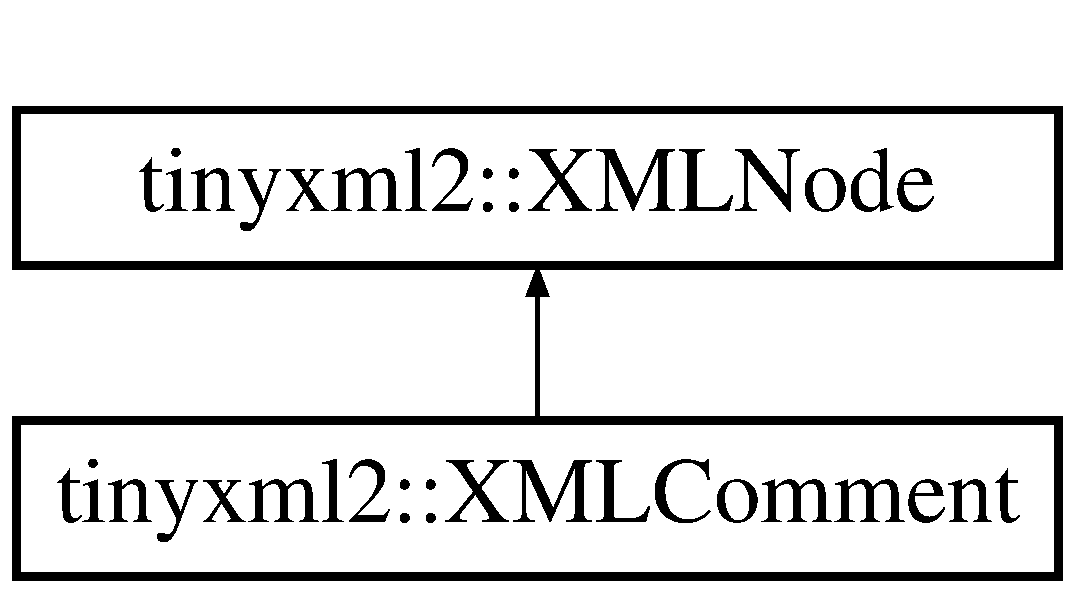
\includegraphics[height=2.000000cm]{classtinyxml2_1_1_x_m_l_comment}
\end{center}
\end{figure}
\subsection*{Public Member Functions}
\begin{DoxyCompactItemize}
\item 
virtual \hyperlink{classtinyxml2_1_1_x_m_l_comment}{X\-M\-L\-Comment} $\ast$ \hyperlink{classtinyxml2_1_1_x_m_l_comment_a8093e1dc8a34fa446d9dc3fde0e6c0ee}{To\-Comment} ()
\begin{DoxyCompactList}\small\item\em Safely cast to a Comment, or null. \end{DoxyCompactList}\item 
virtual const \hyperlink{classtinyxml2_1_1_x_m_l_comment}{X\-M\-L\-Comment} $\ast$ \hyperlink{classtinyxml2_1_1_x_m_l_comment_a422aabac22de7d9c9cad130897dd8b1c}{To\-Comment} () const 
\item 
virtual bool \hyperlink{classtinyxml2_1_1_x_m_l_comment_aa382b1be6a8b0650c16a2d88bb499335}{Accept} (\hyperlink{classtinyxml2_1_1_x_m_l_visitor}{X\-M\-L\-Visitor} $\ast$visitor) const 
\item 
char $\ast$ \hyperlink{classtinyxml2_1_1_x_m_l_comment_aa6ab35c3bb1c1840371dc32a2040c57f}{Parse\-Deep} (char $\ast$, \hyperlink{classtinyxml2_1_1_str_pair}{Str\-Pair} $\ast$end\-Tag)
\item 
virtual \hyperlink{classtinyxml2_1_1_x_m_l_node}{X\-M\-L\-Node} $\ast$ \hyperlink{classtinyxml2_1_1_x_m_l_comment_a90bb60193a691b484f5e1b487857016d}{Shallow\-Clone} (\hyperlink{classtinyxml2_1_1_x_m_l_document}{X\-M\-L\-Document} $\ast$document) const 
\item 
virtual bool \hyperlink{classtinyxml2_1_1_x_m_l_comment_a2d9f26757b0018fce933e74420cda22a}{Shallow\-Equal} (const \hyperlink{classtinyxml2_1_1_x_m_l_node}{X\-M\-L\-Node} $\ast$compare) const 
\end{DoxyCompactItemize}
\subsection*{Protected Member Functions}
\begin{DoxyCompactItemize}
\item 
\hyperlink{classtinyxml2_1_1_x_m_l_comment_ae6463adc3edd93a8e5a9b2b7e99cdf91}{X\-M\-L\-Comment} (\hyperlink{classtinyxml2_1_1_x_m_l_document}{X\-M\-L\-Document} $\ast$doc)
\item 
virtual \hyperlink{classtinyxml2_1_1_x_m_l_comment_ab592f69b47852455c1b32c5e31e453d0}{$\sim$\-X\-M\-L\-Comment} ()
\item 
\hyperlink{classtinyxml2_1_1_x_m_l_comment_aa0a9aae0850ac0e70d3cd20f6cb44447}{X\-M\-L\-Comment} (const \hyperlink{classtinyxml2_1_1_x_m_l_comment}{X\-M\-L\-Comment} \&)
\item 
\hyperlink{classtinyxml2_1_1_x_m_l_comment}{X\-M\-L\-Comment} \& \hyperlink{classtinyxml2_1_1_x_m_l_comment_ac8de55f8381d110740772e6bf6f5755a}{operator=} (const \hyperlink{classtinyxml2_1_1_x_m_l_comment}{X\-M\-L\-Comment} \&)
\end{DoxyCompactItemize}
\subsection*{Friends}
\begin{DoxyCompactItemize}
\item 
class \hyperlink{classtinyxml2_1_1_x_m_l_comment_a4eee3bda60c60a30e4e8cd4ea91c4c6e}{X\-M\-L\-Document}
\end{DoxyCompactItemize}
\subsection*{Additional Inherited Members}


\subsection{Detailed Description}
An X\-M\-L Comment. 

\subsection{Constructor \& Destructor Documentation}
\hypertarget{classtinyxml2_1_1_x_m_l_comment_ae6463adc3edd93a8e5a9b2b7e99cdf91}{\index{tinyxml2\-::\-X\-M\-L\-Comment@{tinyxml2\-::\-X\-M\-L\-Comment}!X\-M\-L\-Comment@{X\-M\-L\-Comment}}
\index{X\-M\-L\-Comment@{X\-M\-L\-Comment}!tinyxml2::XMLComment@{tinyxml2\-::\-X\-M\-L\-Comment}}
\subsubsection[{X\-M\-L\-Comment}]{\setlength{\rightskip}{0pt plus 5cm}tinyxml2\-::\-X\-M\-L\-Comment\-::\-X\-M\-L\-Comment (
\begin{DoxyParamCaption}
\item[{{\bf X\-M\-L\-Document} $\ast$}]{doc}
\end{DoxyParamCaption}
)\hspace{0.3cm}{\ttfamily [protected]}}}\label{classtinyxml2_1_1_x_m_l_comment_ae6463adc3edd93a8e5a9b2b7e99cdf91}
\hypertarget{classtinyxml2_1_1_x_m_l_comment_ab592f69b47852455c1b32c5e31e453d0}{\index{tinyxml2\-::\-X\-M\-L\-Comment@{tinyxml2\-::\-X\-M\-L\-Comment}!$\sim$\-X\-M\-L\-Comment@{$\sim$\-X\-M\-L\-Comment}}
\index{$\sim$\-X\-M\-L\-Comment@{$\sim$\-X\-M\-L\-Comment}!tinyxml2::XMLComment@{tinyxml2\-::\-X\-M\-L\-Comment}}
\subsubsection[{$\sim$\-X\-M\-L\-Comment}]{\setlength{\rightskip}{0pt plus 5cm}tinyxml2\-::\-X\-M\-L\-Comment\-::$\sim$\-X\-M\-L\-Comment (
\begin{DoxyParamCaption}
{}
\end{DoxyParamCaption}
)\hspace{0.3cm}{\ttfamily [protected]}, {\ttfamily [virtual]}}}\label{classtinyxml2_1_1_x_m_l_comment_ab592f69b47852455c1b32c5e31e453d0}
\hypertarget{classtinyxml2_1_1_x_m_l_comment_aa0a9aae0850ac0e70d3cd20f6cb44447}{\index{tinyxml2\-::\-X\-M\-L\-Comment@{tinyxml2\-::\-X\-M\-L\-Comment}!X\-M\-L\-Comment@{X\-M\-L\-Comment}}
\index{X\-M\-L\-Comment@{X\-M\-L\-Comment}!tinyxml2::XMLComment@{tinyxml2\-::\-X\-M\-L\-Comment}}
\subsubsection[{X\-M\-L\-Comment}]{\setlength{\rightskip}{0pt plus 5cm}tinyxml2\-::\-X\-M\-L\-Comment\-::\-X\-M\-L\-Comment (
\begin{DoxyParamCaption}
\item[{const {\bf X\-M\-L\-Comment} \&}]{}
\end{DoxyParamCaption}
)\hspace{0.3cm}{\ttfamily [protected]}}}\label{classtinyxml2_1_1_x_m_l_comment_aa0a9aae0850ac0e70d3cd20f6cb44447}


\subsection{Member Function Documentation}
\hypertarget{classtinyxml2_1_1_x_m_l_comment_aa382b1be6a8b0650c16a2d88bb499335}{\index{tinyxml2\-::\-X\-M\-L\-Comment@{tinyxml2\-::\-X\-M\-L\-Comment}!Accept@{Accept}}
\index{Accept@{Accept}!tinyxml2::XMLComment@{tinyxml2\-::\-X\-M\-L\-Comment}}
\subsubsection[{Accept}]{\setlength{\rightskip}{0pt plus 5cm}bool tinyxml2\-::\-X\-M\-L\-Comment\-::\-Accept (
\begin{DoxyParamCaption}
\item[{{\bf X\-M\-L\-Visitor} $\ast$}]{visitor}
\end{DoxyParamCaption}
) const\hspace{0.3cm}{\ttfamily [virtual]}}}\label{classtinyxml2_1_1_x_m_l_comment_aa382b1be6a8b0650c16a2d88bb499335}
Accept a hierarchical visit of the nodes in the Tiny\-X\-M\-L-\/2 D\-O\-M. Every node in the X\-M\-L tree will be conditionally visited and the host will be called back via the \hyperlink{classtinyxml2_1_1_x_m_l_visitor}{X\-M\-L\-Visitor} interface.

This is essentially a S\-A\-X interface for Tiny\-X\-M\-L-\/2. (Note however it doesn't re-\/parse the X\-M\-L for the callbacks, so the performance of Tiny\-X\-M\-L-\/2 is unchanged by using this interface versus any other.)

The interface has been based on ideas from\-:
\begin{DoxyItemize}
\item \href{http://www.saxproject.org/}{\tt http\-://www.\-saxproject.\-org/}
\item \href{http://c2.com/cgi/wiki?HierarchicalVisitorPattern}{\tt http\-://c2.\-com/cgi/wiki?\-Hierarchical\-Visitor\-Pattern}
\end{DoxyItemize}

Which are both good references for \char`\"{}visiting\char`\"{}.

An example of using \hyperlink{classtinyxml2_1_1_x_m_l_comment_aa382b1be6a8b0650c16a2d88bb499335}{Accept()}\-: \begin{DoxyVerb}XMLPrinter printer;
tinyxmlDoc.Accept( &printer );
const char* xmlcstr = printer.CStr();
\end{DoxyVerb}
 

Implements \hyperlink{classtinyxml2_1_1_x_m_l_node_a81e66df0a44c67a7af17f3b77a152785}{tinyxml2\-::\-X\-M\-L\-Node}.

\hypertarget{classtinyxml2_1_1_x_m_l_comment_ac8de55f8381d110740772e6bf6f5755a}{\index{tinyxml2\-::\-X\-M\-L\-Comment@{tinyxml2\-::\-X\-M\-L\-Comment}!operator=@{operator=}}
\index{operator=@{operator=}!tinyxml2::XMLComment@{tinyxml2\-::\-X\-M\-L\-Comment}}
\subsubsection[{operator=}]{\setlength{\rightskip}{0pt plus 5cm}{\bf X\-M\-L\-Comment}\& tinyxml2\-::\-X\-M\-L\-Comment\-::operator= (
\begin{DoxyParamCaption}
\item[{const {\bf X\-M\-L\-Comment} \&}]{}
\end{DoxyParamCaption}
)\hspace{0.3cm}{\ttfamily [protected]}}}\label{classtinyxml2_1_1_x_m_l_comment_ac8de55f8381d110740772e6bf6f5755a}
\hypertarget{classtinyxml2_1_1_x_m_l_comment_aa6ab35c3bb1c1840371dc32a2040c57f}{\index{tinyxml2\-::\-X\-M\-L\-Comment@{tinyxml2\-::\-X\-M\-L\-Comment}!Parse\-Deep@{Parse\-Deep}}
\index{Parse\-Deep@{Parse\-Deep}!tinyxml2::XMLComment@{tinyxml2\-::\-X\-M\-L\-Comment}}
\subsubsection[{Parse\-Deep}]{\setlength{\rightskip}{0pt plus 5cm}char $\ast$ tinyxml2\-::\-X\-M\-L\-Comment\-::\-Parse\-Deep (
\begin{DoxyParamCaption}
\item[{char $\ast$}]{p, }
\item[{{\bf Str\-Pair} $\ast$}]{end\-Tag}
\end{DoxyParamCaption}
)\hspace{0.3cm}{\ttfamily [virtual]}}}\label{classtinyxml2_1_1_x_m_l_comment_aa6ab35c3bb1c1840371dc32a2040c57f}


Reimplemented from \hyperlink{classtinyxml2_1_1_x_m_l_node_a7610d0f603e8b603d2078521811a23c1}{tinyxml2\-::\-X\-M\-L\-Node}.

\hypertarget{classtinyxml2_1_1_x_m_l_comment_a90bb60193a691b484f5e1b487857016d}{\index{tinyxml2\-::\-X\-M\-L\-Comment@{tinyxml2\-::\-X\-M\-L\-Comment}!Shallow\-Clone@{Shallow\-Clone}}
\index{Shallow\-Clone@{Shallow\-Clone}!tinyxml2::XMLComment@{tinyxml2\-::\-X\-M\-L\-Comment}}
\subsubsection[{Shallow\-Clone}]{\setlength{\rightskip}{0pt plus 5cm}{\bf X\-M\-L\-Node} $\ast$ tinyxml2\-::\-X\-M\-L\-Comment\-::\-Shallow\-Clone (
\begin{DoxyParamCaption}
\item[{{\bf X\-M\-L\-Document} $\ast$}]{document}
\end{DoxyParamCaption}
) const\hspace{0.3cm}{\ttfamily [virtual]}}}\label{classtinyxml2_1_1_x_m_l_comment_a90bb60193a691b484f5e1b487857016d}
Make a copy of this node, but not its children. You may pass in a Document pointer that will be the owner of the new Node. If the 'document' is null, then the node returned will be allocated from the current Document. (this-\/$>$\hyperlink{classtinyxml2_1_1_x_m_l_node_af343d1ef0b45c0020e62d784d7e67a68}{Get\-Document()})

Note\-: if called on a \hyperlink{classtinyxml2_1_1_x_m_l_document}{X\-M\-L\-Document}, this will return null. 

Implements \hyperlink{classtinyxml2_1_1_x_m_l_node_a8402cbd3129d20e9e6024bbcc0531283}{tinyxml2\-::\-X\-M\-L\-Node}.

\hypertarget{classtinyxml2_1_1_x_m_l_comment_a2d9f26757b0018fce933e74420cda22a}{\index{tinyxml2\-::\-X\-M\-L\-Comment@{tinyxml2\-::\-X\-M\-L\-Comment}!Shallow\-Equal@{Shallow\-Equal}}
\index{Shallow\-Equal@{Shallow\-Equal}!tinyxml2::XMLComment@{tinyxml2\-::\-X\-M\-L\-Comment}}
\subsubsection[{Shallow\-Equal}]{\setlength{\rightskip}{0pt plus 5cm}bool tinyxml2\-::\-X\-M\-L\-Comment\-::\-Shallow\-Equal (
\begin{DoxyParamCaption}
\item[{const {\bf X\-M\-L\-Node} $\ast$}]{compare}
\end{DoxyParamCaption}
) const\hspace{0.3cm}{\ttfamily [virtual]}}}\label{classtinyxml2_1_1_x_m_l_comment_a2d9f26757b0018fce933e74420cda22a}
Test if 2 nodes are the same, but don't test children. The 2 nodes do not need to be in the same Document.

Note\-: if called on a \hyperlink{classtinyxml2_1_1_x_m_l_document}{X\-M\-L\-Document}, this will return false. 

Implements \hyperlink{classtinyxml2_1_1_x_m_l_node_a7ce18b751c3ea09eac292dca264f9226}{tinyxml2\-::\-X\-M\-L\-Node}.

\hypertarget{classtinyxml2_1_1_x_m_l_comment_a8093e1dc8a34fa446d9dc3fde0e6c0ee}{\index{tinyxml2\-::\-X\-M\-L\-Comment@{tinyxml2\-::\-X\-M\-L\-Comment}!To\-Comment@{To\-Comment}}
\index{To\-Comment@{To\-Comment}!tinyxml2::XMLComment@{tinyxml2\-::\-X\-M\-L\-Comment}}
\subsubsection[{To\-Comment}]{\setlength{\rightskip}{0pt plus 5cm}virtual {\bf X\-M\-L\-Comment}$\ast$ tinyxml2\-::\-X\-M\-L\-Comment\-::\-To\-Comment (
\begin{DoxyParamCaption}
{}
\end{DoxyParamCaption}
)\hspace{0.3cm}{\ttfamily [inline]}, {\ttfamily [virtual]}}}\label{classtinyxml2_1_1_x_m_l_comment_a8093e1dc8a34fa446d9dc3fde0e6c0ee}


Safely cast to a Comment, or null. 



Reimplemented from \hyperlink{classtinyxml2_1_1_x_m_l_node_aff47671055aa99840a1c1ebd661e63e3}{tinyxml2\-::\-X\-M\-L\-Node}.

\hypertarget{classtinyxml2_1_1_x_m_l_comment_a422aabac22de7d9c9cad130897dd8b1c}{\index{tinyxml2\-::\-X\-M\-L\-Comment@{tinyxml2\-::\-X\-M\-L\-Comment}!To\-Comment@{To\-Comment}}
\index{To\-Comment@{To\-Comment}!tinyxml2::XMLComment@{tinyxml2\-::\-X\-M\-L\-Comment}}
\subsubsection[{To\-Comment}]{\setlength{\rightskip}{0pt plus 5cm}virtual const {\bf X\-M\-L\-Comment}$\ast$ tinyxml2\-::\-X\-M\-L\-Comment\-::\-To\-Comment (
\begin{DoxyParamCaption}
{}
\end{DoxyParamCaption}
) const\hspace{0.3cm}{\ttfamily [inline]}, {\ttfamily [virtual]}}}\label{classtinyxml2_1_1_x_m_l_comment_a422aabac22de7d9c9cad130897dd8b1c}


Reimplemented from \hyperlink{classtinyxml2_1_1_x_m_l_node_a157ce3a00ea5ee5a85b7103138e85e8a}{tinyxml2\-::\-X\-M\-L\-Node}.



\subsection{Friends And Related Function Documentation}
\hypertarget{classtinyxml2_1_1_x_m_l_comment_a4eee3bda60c60a30e4e8cd4ea91c4c6e}{\index{tinyxml2\-::\-X\-M\-L\-Comment@{tinyxml2\-::\-X\-M\-L\-Comment}!X\-M\-L\-Document@{X\-M\-L\-Document}}
\index{X\-M\-L\-Document@{X\-M\-L\-Document}!tinyxml2::XMLComment@{tinyxml2\-::\-X\-M\-L\-Comment}}
\subsubsection[{X\-M\-L\-Document}]{\setlength{\rightskip}{0pt plus 5cm}friend class {\bf X\-M\-L\-Document}\hspace{0.3cm}{\ttfamily [friend]}}}\label{classtinyxml2_1_1_x_m_l_comment_a4eee3bda60c60a30e4e8cd4ea91c4c6e}


The documentation for this class was generated from the following files\-:\begin{DoxyCompactItemize}
\item 
Utils/\-X\-M\-L\-\_\-\-Config/\hyperlink{tinyxml2_8h}{tinyxml2.\-h}\item 
Utils/\-X\-M\-L\-\_\-\-Config/\hyperlink{tinyxml2_8cpp}{tinyxml2.\-cpp}\end{DoxyCompactItemize}

\hypertarget{classtinyxml2_1_1_x_m_l_const_handle}{\section{tinyxml2\-:\-:X\-M\-L\-Const\-Handle Class Reference}
\label{classtinyxml2_1_1_x_m_l_const_handle}\index{tinyxml2\-::\-X\-M\-L\-Const\-Handle@{tinyxml2\-::\-X\-M\-L\-Const\-Handle}}
}


{\ttfamily \#include $<$tinyxml2.\-h$>$}

\subsection*{Public Member Functions}
\begin{DoxyCompactItemize}
\item 
\hyperlink{classtinyxml2_1_1_x_m_l_const_handle_a098bda71fa11d7c74ccddab59d5dd534}{X\-M\-L\-Const\-Handle} (const \hyperlink{classtinyxml2_1_1_x_m_l_node}{X\-M\-L\-Node} $\ast$node)
\item 
\hyperlink{classtinyxml2_1_1_x_m_l_const_handle_a8420a0c4720637e0529e78c2e22f2b0b}{X\-M\-L\-Const\-Handle} (const \hyperlink{classtinyxml2_1_1_x_m_l_node}{X\-M\-L\-Node} \&node)
\item 
\hyperlink{classtinyxml2_1_1_x_m_l_const_handle_a639317ad315ff24f4ef0dc69312d7303}{X\-M\-L\-Const\-Handle} (const \hyperlink{classtinyxml2_1_1_x_m_l_const_handle}{X\-M\-L\-Const\-Handle} \&ref)
\item 
\hyperlink{classtinyxml2_1_1_x_m_l_const_handle}{X\-M\-L\-Const\-Handle} \& \hyperlink{classtinyxml2_1_1_x_m_l_const_handle_a2d74c91df1ff9aa5f9b57e3dceddbf94}{operator=} (const \hyperlink{classtinyxml2_1_1_x_m_l_const_handle}{X\-M\-L\-Const\-Handle} \&ref)
\item 
const \hyperlink{classtinyxml2_1_1_x_m_l_const_handle}{X\-M\-L\-Const\-Handle} \hyperlink{classtinyxml2_1_1_x_m_l_const_handle_a64c4ff7074effc1fd181d68d23f9d1e4}{First\-Child} () const 
\item 
const \hyperlink{classtinyxml2_1_1_x_m_l_const_handle}{X\-M\-L\-Const\-Handle} \hyperlink{classtinyxml2_1_1_x_m_l_const_handle_a5c197d0b57f8e560d93356a4a281469c}{First\-Child\-Element} (const char $\ast$value=0) const 
\item 
const \hyperlink{classtinyxml2_1_1_x_m_l_const_handle}{X\-M\-L\-Const\-Handle} \hyperlink{classtinyxml2_1_1_x_m_l_const_handle_afec9a68e7951193bc5a6e876d602f263}{Last\-Child} () const 
\item 
const \hyperlink{classtinyxml2_1_1_x_m_l_const_handle}{X\-M\-L\-Const\-Handle} \hyperlink{classtinyxml2_1_1_x_m_l_const_handle_a1c400e66dace6fdab4927adb21090059}{Last\-Child\-Element} (const char $\ast$\-\_\-value=0) const 
\item 
const \hyperlink{classtinyxml2_1_1_x_m_l_const_handle}{X\-M\-L\-Const\-Handle} \hyperlink{classtinyxml2_1_1_x_m_l_const_handle_a6917564e26b2c20ebdcb23c7940ad80a}{Previous\-Sibling} () const 
\item 
const \hyperlink{classtinyxml2_1_1_x_m_l_const_handle}{X\-M\-L\-Const\-Handle} \hyperlink{classtinyxml2_1_1_x_m_l_const_handle_acb2e1c5762eff9f6ed72d1a2dfc14271}{Previous\-Sibling\-Element} (const char $\ast$\-\_\-value=0) const 
\item 
const \hyperlink{classtinyxml2_1_1_x_m_l_const_handle}{X\-M\-L\-Const\-Handle} \hyperlink{classtinyxml2_1_1_x_m_l_const_handle_a596e248c8014d718f41658502a2e221b}{Next\-Sibling} () const 
\item 
const \hyperlink{classtinyxml2_1_1_x_m_l_const_handle}{X\-M\-L\-Const\-Handle} \hyperlink{classtinyxml2_1_1_x_m_l_const_handle_a3bbdd3d866c750473bd69a232704503b}{Next\-Sibling\-Element} (const char $\ast$\-\_\-value=0) const 
\item 
const \hyperlink{classtinyxml2_1_1_x_m_l_node}{X\-M\-L\-Node} $\ast$ \hyperlink{classtinyxml2_1_1_x_m_l_const_handle_a95d0256318c10c3f75fa5f8ffb3e4bc1}{To\-Node} () const 
\item 
const \hyperlink{classtinyxml2_1_1_x_m_l_element}{X\-M\-L\-Element} $\ast$ \hyperlink{classtinyxml2_1_1_x_m_l_const_handle_a5a48adefc2a5e70d4ce5b55692a0e2f9}{To\-Element} () const 
\item 
const \hyperlink{classtinyxml2_1_1_x_m_l_text}{X\-M\-L\-Text} $\ast$ \hyperlink{classtinyxml2_1_1_x_m_l_const_handle_ad86ca7dbb20d0495ae357fe7a866e0be}{To\-Text} () const 
\item 
const \hyperlink{classtinyxml2_1_1_x_m_l_unknown}{X\-M\-L\-Unknown} $\ast$ \hyperlink{classtinyxml2_1_1_x_m_l_const_handle_acb358a329e54fa204ed2d0b181566828}{To\-Unknown} () const 
\item 
const \hyperlink{classtinyxml2_1_1_x_m_l_declaration}{X\-M\-L\-Declaration} $\ast$ \hyperlink{classtinyxml2_1_1_x_m_l_const_handle_a5de0c175845bc30a6f9b3d88d8877eaf}{To\-Declaration} () const 
\end{DoxyCompactItemize}
\subsection*{Private Attributes}
\begin{DoxyCompactItemize}
\item 
const \hyperlink{classtinyxml2_1_1_x_m_l_node}{X\-M\-L\-Node} $\ast$ \hyperlink{classtinyxml2_1_1_x_m_l_const_handle_ad4d8db839660ef730adfa2439945c4da}{\-\_\-node}
\end{DoxyCompactItemize}


\subsection{Detailed Description}
A variant of the \hyperlink{classtinyxml2_1_1_x_m_l_handle}{X\-M\-L\-Handle} class for working with const X\-M\-L\-Nodes and Documents. It is the same in all regards, except for the 'const' qualifiers. See \hyperlink{classtinyxml2_1_1_x_m_l_handle}{X\-M\-L\-Handle} for A\-P\-I. 

\subsection{Constructor \& Destructor Documentation}
\hypertarget{classtinyxml2_1_1_x_m_l_const_handle_a098bda71fa11d7c74ccddab59d5dd534}{\index{tinyxml2\-::\-X\-M\-L\-Const\-Handle@{tinyxml2\-::\-X\-M\-L\-Const\-Handle}!X\-M\-L\-Const\-Handle@{X\-M\-L\-Const\-Handle}}
\index{X\-M\-L\-Const\-Handle@{X\-M\-L\-Const\-Handle}!tinyxml2::XMLConstHandle@{tinyxml2\-::\-X\-M\-L\-Const\-Handle}}
\subsubsection[{X\-M\-L\-Const\-Handle}]{\setlength{\rightskip}{0pt plus 5cm}tinyxml2\-::\-X\-M\-L\-Const\-Handle\-::\-X\-M\-L\-Const\-Handle (
\begin{DoxyParamCaption}
\item[{const {\bf X\-M\-L\-Node} $\ast$}]{node}
\end{DoxyParamCaption}
)\hspace{0.3cm}{\ttfamily [inline]}}}\label{classtinyxml2_1_1_x_m_l_const_handle_a098bda71fa11d7c74ccddab59d5dd534}
\hypertarget{classtinyxml2_1_1_x_m_l_const_handle_a8420a0c4720637e0529e78c2e22f2b0b}{\index{tinyxml2\-::\-X\-M\-L\-Const\-Handle@{tinyxml2\-::\-X\-M\-L\-Const\-Handle}!X\-M\-L\-Const\-Handle@{X\-M\-L\-Const\-Handle}}
\index{X\-M\-L\-Const\-Handle@{X\-M\-L\-Const\-Handle}!tinyxml2::XMLConstHandle@{tinyxml2\-::\-X\-M\-L\-Const\-Handle}}
\subsubsection[{X\-M\-L\-Const\-Handle}]{\setlength{\rightskip}{0pt plus 5cm}tinyxml2\-::\-X\-M\-L\-Const\-Handle\-::\-X\-M\-L\-Const\-Handle (
\begin{DoxyParamCaption}
\item[{const {\bf X\-M\-L\-Node} \&}]{node}
\end{DoxyParamCaption}
)\hspace{0.3cm}{\ttfamily [inline]}}}\label{classtinyxml2_1_1_x_m_l_const_handle_a8420a0c4720637e0529e78c2e22f2b0b}
\hypertarget{classtinyxml2_1_1_x_m_l_const_handle_a639317ad315ff24f4ef0dc69312d7303}{\index{tinyxml2\-::\-X\-M\-L\-Const\-Handle@{tinyxml2\-::\-X\-M\-L\-Const\-Handle}!X\-M\-L\-Const\-Handle@{X\-M\-L\-Const\-Handle}}
\index{X\-M\-L\-Const\-Handle@{X\-M\-L\-Const\-Handle}!tinyxml2::XMLConstHandle@{tinyxml2\-::\-X\-M\-L\-Const\-Handle}}
\subsubsection[{X\-M\-L\-Const\-Handle}]{\setlength{\rightskip}{0pt plus 5cm}tinyxml2\-::\-X\-M\-L\-Const\-Handle\-::\-X\-M\-L\-Const\-Handle (
\begin{DoxyParamCaption}
\item[{const {\bf X\-M\-L\-Const\-Handle} \&}]{ref}
\end{DoxyParamCaption}
)\hspace{0.3cm}{\ttfamily [inline]}}}\label{classtinyxml2_1_1_x_m_l_const_handle_a639317ad315ff24f4ef0dc69312d7303}


\subsection{Member Function Documentation}
\hypertarget{classtinyxml2_1_1_x_m_l_const_handle_a64c4ff7074effc1fd181d68d23f9d1e4}{\index{tinyxml2\-::\-X\-M\-L\-Const\-Handle@{tinyxml2\-::\-X\-M\-L\-Const\-Handle}!First\-Child@{First\-Child}}
\index{First\-Child@{First\-Child}!tinyxml2::XMLConstHandle@{tinyxml2\-::\-X\-M\-L\-Const\-Handle}}
\subsubsection[{First\-Child}]{\setlength{\rightskip}{0pt plus 5cm}const {\bf X\-M\-L\-Const\-Handle} tinyxml2\-::\-X\-M\-L\-Const\-Handle\-::\-First\-Child (
\begin{DoxyParamCaption}
{}
\end{DoxyParamCaption}
) const\hspace{0.3cm}{\ttfamily [inline]}}}\label{classtinyxml2_1_1_x_m_l_const_handle_a64c4ff7074effc1fd181d68d23f9d1e4}
\hypertarget{classtinyxml2_1_1_x_m_l_const_handle_a5c197d0b57f8e560d93356a4a281469c}{\index{tinyxml2\-::\-X\-M\-L\-Const\-Handle@{tinyxml2\-::\-X\-M\-L\-Const\-Handle}!First\-Child\-Element@{First\-Child\-Element}}
\index{First\-Child\-Element@{First\-Child\-Element}!tinyxml2::XMLConstHandle@{tinyxml2\-::\-X\-M\-L\-Const\-Handle}}
\subsubsection[{First\-Child\-Element}]{\setlength{\rightskip}{0pt plus 5cm}const {\bf X\-M\-L\-Const\-Handle} tinyxml2\-::\-X\-M\-L\-Const\-Handle\-::\-First\-Child\-Element (
\begin{DoxyParamCaption}
\item[{const char $\ast$}]{value = {\ttfamily 0}}
\end{DoxyParamCaption}
) const\hspace{0.3cm}{\ttfamily [inline]}}}\label{classtinyxml2_1_1_x_m_l_const_handle_a5c197d0b57f8e560d93356a4a281469c}
\hypertarget{classtinyxml2_1_1_x_m_l_const_handle_afec9a68e7951193bc5a6e876d602f263}{\index{tinyxml2\-::\-X\-M\-L\-Const\-Handle@{tinyxml2\-::\-X\-M\-L\-Const\-Handle}!Last\-Child@{Last\-Child}}
\index{Last\-Child@{Last\-Child}!tinyxml2::XMLConstHandle@{tinyxml2\-::\-X\-M\-L\-Const\-Handle}}
\subsubsection[{Last\-Child}]{\setlength{\rightskip}{0pt plus 5cm}const {\bf X\-M\-L\-Const\-Handle} tinyxml2\-::\-X\-M\-L\-Const\-Handle\-::\-Last\-Child (
\begin{DoxyParamCaption}
{}
\end{DoxyParamCaption}
) const\hspace{0.3cm}{\ttfamily [inline]}}}\label{classtinyxml2_1_1_x_m_l_const_handle_afec9a68e7951193bc5a6e876d602f263}
\hypertarget{classtinyxml2_1_1_x_m_l_const_handle_a1c400e66dace6fdab4927adb21090059}{\index{tinyxml2\-::\-X\-M\-L\-Const\-Handle@{tinyxml2\-::\-X\-M\-L\-Const\-Handle}!Last\-Child\-Element@{Last\-Child\-Element}}
\index{Last\-Child\-Element@{Last\-Child\-Element}!tinyxml2::XMLConstHandle@{tinyxml2\-::\-X\-M\-L\-Const\-Handle}}
\subsubsection[{Last\-Child\-Element}]{\setlength{\rightskip}{0pt plus 5cm}const {\bf X\-M\-L\-Const\-Handle} tinyxml2\-::\-X\-M\-L\-Const\-Handle\-::\-Last\-Child\-Element (
\begin{DoxyParamCaption}
\item[{const char $\ast$}]{\-\_\-value = {\ttfamily 0}}
\end{DoxyParamCaption}
) const\hspace{0.3cm}{\ttfamily [inline]}}}\label{classtinyxml2_1_1_x_m_l_const_handle_a1c400e66dace6fdab4927adb21090059}
\hypertarget{classtinyxml2_1_1_x_m_l_const_handle_a596e248c8014d718f41658502a2e221b}{\index{tinyxml2\-::\-X\-M\-L\-Const\-Handle@{tinyxml2\-::\-X\-M\-L\-Const\-Handle}!Next\-Sibling@{Next\-Sibling}}
\index{Next\-Sibling@{Next\-Sibling}!tinyxml2::XMLConstHandle@{tinyxml2\-::\-X\-M\-L\-Const\-Handle}}
\subsubsection[{Next\-Sibling}]{\setlength{\rightskip}{0pt plus 5cm}const {\bf X\-M\-L\-Const\-Handle} tinyxml2\-::\-X\-M\-L\-Const\-Handle\-::\-Next\-Sibling (
\begin{DoxyParamCaption}
{}
\end{DoxyParamCaption}
) const\hspace{0.3cm}{\ttfamily [inline]}}}\label{classtinyxml2_1_1_x_m_l_const_handle_a596e248c8014d718f41658502a2e221b}
\hypertarget{classtinyxml2_1_1_x_m_l_const_handle_a3bbdd3d866c750473bd69a232704503b}{\index{tinyxml2\-::\-X\-M\-L\-Const\-Handle@{tinyxml2\-::\-X\-M\-L\-Const\-Handle}!Next\-Sibling\-Element@{Next\-Sibling\-Element}}
\index{Next\-Sibling\-Element@{Next\-Sibling\-Element}!tinyxml2::XMLConstHandle@{tinyxml2\-::\-X\-M\-L\-Const\-Handle}}
\subsubsection[{Next\-Sibling\-Element}]{\setlength{\rightskip}{0pt plus 5cm}const {\bf X\-M\-L\-Const\-Handle} tinyxml2\-::\-X\-M\-L\-Const\-Handle\-::\-Next\-Sibling\-Element (
\begin{DoxyParamCaption}
\item[{const char $\ast$}]{\-\_\-value = {\ttfamily 0}}
\end{DoxyParamCaption}
) const\hspace{0.3cm}{\ttfamily [inline]}}}\label{classtinyxml2_1_1_x_m_l_const_handle_a3bbdd3d866c750473bd69a232704503b}
\hypertarget{classtinyxml2_1_1_x_m_l_const_handle_a2d74c91df1ff9aa5f9b57e3dceddbf94}{\index{tinyxml2\-::\-X\-M\-L\-Const\-Handle@{tinyxml2\-::\-X\-M\-L\-Const\-Handle}!operator=@{operator=}}
\index{operator=@{operator=}!tinyxml2::XMLConstHandle@{tinyxml2\-::\-X\-M\-L\-Const\-Handle}}
\subsubsection[{operator=}]{\setlength{\rightskip}{0pt plus 5cm}{\bf X\-M\-L\-Const\-Handle}\& tinyxml2\-::\-X\-M\-L\-Const\-Handle\-::operator= (
\begin{DoxyParamCaption}
\item[{const {\bf X\-M\-L\-Const\-Handle} \&}]{ref}
\end{DoxyParamCaption}
)\hspace{0.3cm}{\ttfamily [inline]}}}\label{classtinyxml2_1_1_x_m_l_const_handle_a2d74c91df1ff9aa5f9b57e3dceddbf94}
\hypertarget{classtinyxml2_1_1_x_m_l_const_handle_a6917564e26b2c20ebdcb23c7940ad80a}{\index{tinyxml2\-::\-X\-M\-L\-Const\-Handle@{tinyxml2\-::\-X\-M\-L\-Const\-Handle}!Previous\-Sibling@{Previous\-Sibling}}
\index{Previous\-Sibling@{Previous\-Sibling}!tinyxml2::XMLConstHandle@{tinyxml2\-::\-X\-M\-L\-Const\-Handle}}
\subsubsection[{Previous\-Sibling}]{\setlength{\rightskip}{0pt plus 5cm}const {\bf X\-M\-L\-Const\-Handle} tinyxml2\-::\-X\-M\-L\-Const\-Handle\-::\-Previous\-Sibling (
\begin{DoxyParamCaption}
{}
\end{DoxyParamCaption}
) const\hspace{0.3cm}{\ttfamily [inline]}}}\label{classtinyxml2_1_1_x_m_l_const_handle_a6917564e26b2c20ebdcb23c7940ad80a}
\hypertarget{classtinyxml2_1_1_x_m_l_const_handle_acb2e1c5762eff9f6ed72d1a2dfc14271}{\index{tinyxml2\-::\-X\-M\-L\-Const\-Handle@{tinyxml2\-::\-X\-M\-L\-Const\-Handle}!Previous\-Sibling\-Element@{Previous\-Sibling\-Element}}
\index{Previous\-Sibling\-Element@{Previous\-Sibling\-Element}!tinyxml2::XMLConstHandle@{tinyxml2\-::\-X\-M\-L\-Const\-Handle}}
\subsubsection[{Previous\-Sibling\-Element}]{\setlength{\rightskip}{0pt plus 5cm}const {\bf X\-M\-L\-Const\-Handle} tinyxml2\-::\-X\-M\-L\-Const\-Handle\-::\-Previous\-Sibling\-Element (
\begin{DoxyParamCaption}
\item[{const char $\ast$}]{\-\_\-value = {\ttfamily 0}}
\end{DoxyParamCaption}
) const\hspace{0.3cm}{\ttfamily [inline]}}}\label{classtinyxml2_1_1_x_m_l_const_handle_acb2e1c5762eff9f6ed72d1a2dfc14271}
\hypertarget{classtinyxml2_1_1_x_m_l_const_handle_a5de0c175845bc30a6f9b3d88d8877eaf}{\index{tinyxml2\-::\-X\-M\-L\-Const\-Handle@{tinyxml2\-::\-X\-M\-L\-Const\-Handle}!To\-Declaration@{To\-Declaration}}
\index{To\-Declaration@{To\-Declaration}!tinyxml2::XMLConstHandle@{tinyxml2\-::\-X\-M\-L\-Const\-Handle}}
\subsubsection[{To\-Declaration}]{\setlength{\rightskip}{0pt plus 5cm}const {\bf X\-M\-L\-Declaration}$\ast$ tinyxml2\-::\-X\-M\-L\-Const\-Handle\-::\-To\-Declaration (
\begin{DoxyParamCaption}
{}
\end{DoxyParamCaption}
) const\hspace{0.3cm}{\ttfamily [inline]}}}\label{classtinyxml2_1_1_x_m_l_const_handle_a5de0c175845bc30a6f9b3d88d8877eaf}
\hypertarget{classtinyxml2_1_1_x_m_l_const_handle_a5a48adefc2a5e70d4ce5b55692a0e2f9}{\index{tinyxml2\-::\-X\-M\-L\-Const\-Handle@{tinyxml2\-::\-X\-M\-L\-Const\-Handle}!To\-Element@{To\-Element}}
\index{To\-Element@{To\-Element}!tinyxml2::XMLConstHandle@{tinyxml2\-::\-X\-M\-L\-Const\-Handle}}
\subsubsection[{To\-Element}]{\setlength{\rightskip}{0pt plus 5cm}const {\bf X\-M\-L\-Element}$\ast$ tinyxml2\-::\-X\-M\-L\-Const\-Handle\-::\-To\-Element (
\begin{DoxyParamCaption}
{}
\end{DoxyParamCaption}
) const\hspace{0.3cm}{\ttfamily [inline]}}}\label{classtinyxml2_1_1_x_m_l_const_handle_a5a48adefc2a5e70d4ce5b55692a0e2f9}
\hypertarget{classtinyxml2_1_1_x_m_l_const_handle_a95d0256318c10c3f75fa5f8ffb3e4bc1}{\index{tinyxml2\-::\-X\-M\-L\-Const\-Handle@{tinyxml2\-::\-X\-M\-L\-Const\-Handle}!To\-Node@{To\-Node}}
\index{To\-Node@{To\-Node}!tinyxml2::XMLConstHandle@{tinyxml2\-::\-X\-M\-L\-Const\-Handle}}
\subsubsection[{To\-Node}]{\setlength{\rightskip}{0pt plus 5cm}const {\bf X\-M\-L\-Node}$\ast$ tinyxml2\-::\-X\-M\-L\-Const\-Handle\-::\-To\-Node (
\begin{DoxyParamCaption}
{}
\end{DoxyParamCaption}
) const\hspace{0.3cm}{\ttfamily [inline]}}}\label{classtinyxml2_1_1_x_m_l_const_handle_a95d0256318c10c3f75fa5f8ffb3e4bc1}
\hypertarget{classtinyxml2_1_1_x_m_l_const_handle_ad86ca7dbb20d0495ae357fe7a866e0be}{\index{tinyxml2\-::\-X\-M\-L\-Const\-Handle@{tinyxml2\-::\-X\-M\-L\-Const\-Handle}!To\-Text@{To\-Text}}
\index{To\-Text@{To\-Text}!tinyxml2::XMLConstHandle@{tinyxml2\-::\-X\-M\-L\-Const\-Handle}}
\subsubsection[{To\-Text}]{\setlength{\rightskip}{0pt plus 5cm}const {\bf X\-M\-L\-Text}$\ast$ tinyxml2\-::\-X\-M\-L\-Const\-Handle\-::\-To\-Text (
\begin{DoxyParamCaption}
{}
\end{DoxyParamCaption}
) const\hspace{0.3cm}{\ttfamily [inline]}}}\label{classtinyxml2_1_1_x_m_l_const_handle_ad86ca7dbb20d0495ae357fe7a866e0be}
\hypertarget{classtinyxml2_1_1_x_m_l_const_handle_acb358a329e54fa204ed2d0b181566828}{\index{tinyxml2\-::\-X\-M\-L\-Const\-Handle@{tinyxml2\-::\-X\-M\-L\-Const\-Handle}!To\-Unknown@{To\-Unknown}}
\index{To\-Unknown@{To\-Unknown}!tinyxml2::XMLConstHandle@{tinyxml2\-::\-X\-M\-L\-Const\-Handle}}
\subsubsection[{To\-Unknown}]{\setlength{\rightskip}{0pt plus 5cm}const {\bf X\-M\-L\-Unknown}$\ast$ tinyxml2\-::\-X\-M\-L\-Const\-Handle\-::\-To\-Unknown (
\begin{DoxyParamCaption}
{}
\end{DoxyParamCaption}
) const\hspace{0.3cm}{\ttfamily [inline]}}}\label{classtinyxml2_1_1_x_m_l_const_handle_acb358a329e54fa204ed2d0b181566828}


\subsection{Member Data Documentation}
\hypertarget{classtinyxml2_1_1_x_m_l_const_handle_ad4d8db839660ef730adfa2439945c4da}{\index{tinyxml2\-::\-X\-M\-L\-Const\-Handle@{tinyxml2\-::\-X\-M\-L\-Const\-Handle}!\-\_\-node@{\-\_\-node}}
\index{\-\_\-node@{\-\_\-node}!tinyxml2::XMLConstHandle@{tinyxml2\-::\-X\-M\-L\-Const\-Handle}}
\subsubsection[{\-\_\-node}]{\setlength{\rightskip}{0pt plus 5cm}const {\bf X\-M\-L\-Node}$\ast$ tinyxml2\-::\-X\-M\-L\-Const\-Handle\-::\-\_\-node\hspace{0.3cm}{\ttfamily [private]}}}\label{classtinyxml2_1_1_x_m_l_const_handle_ad4d8db839660ef730adfa2439945c4da}


The documentation for this class was generated from the following file\-:\begin{DoxyCompactItemize}
\item 
Utils/\-X\-M\-L\-\_\-\-Config/\hyperlink{tinyxml2_8h}{tinyxml2.\-h}\end{DoxyCompactItemize}

\hypertarget{classtinyxml2_1_1_x_m_l_declaration}{\section{tinyxml2\-:\-:X\-M\-L\-Declaration Class Reference}
\label{classtinyxml2_1_1_x_m_l_declaration}\index{tinyxml2\-::\-X\-M\-L\-Declaration@{tinyxml2\-::\-X\-M\-L\-Declaration}}
}


{\ttfamily \#include $<$tinyxml2.\-h$>$}

Inheritance diagram for tinyxml2\-:\-:X\-M\-L\-Declaration\-:\begin{figure}[H]
\begin{center}
\leavevmode
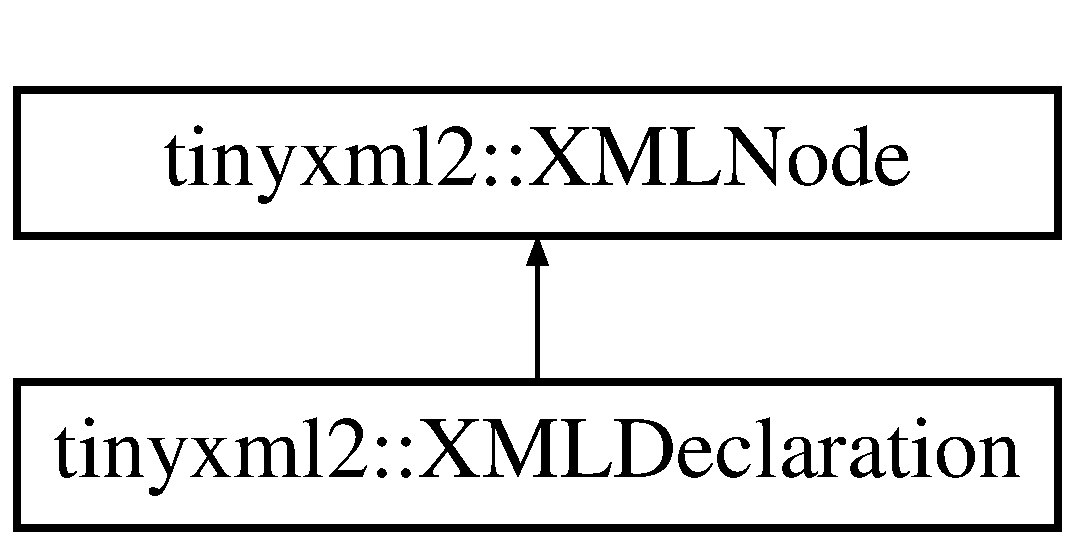
\includegraphics[height=2.000000cm]{classtinyxml2_1_1_x_m_l_declaration}
\end{center}
\end{figure}
\subsection*{Public Member Functions}
\begin{DoxyCompactItemize}
\item 
virtual \hyperlink{classtinyxml2_1_1_x_m_l_declaration}{X\-M\-L\-Declaration} $\ast$ \hyperlink{classtinyxml2_1_1_x_m_l_declaration_a159d8ac45865215e88059ea1e5b52fc5}{To\-Declaration} ()
\begin{DoxyCompactList}\small\item\em Safely cast to a Declaration, or null. \end{DoxyCompactList}\item 
virtual const \hyperlink{classtinyxml2_1_1_x_m_l_declaration}{X\-M\-L\-Declaration} $\ast$ \hyperlink{classtinyxml2_1_1_x_m_l_declaration_af724607a5fa810496fd6a21f5975a643}{To\-Declaration} () const 
\item 
virtual bool \hyperlink{classtinyxml2_1_1_x_m_l_declaration_a953a7359cc312d15218eb5843a4ca108}{Accept} (\hyperlink{classtinyxml2_1_1_x_m_l_visitor}{X\-M\-L\-Visitor} $\ast$visitor) const 
\item 
char $\ast$ \hyperlink{classtinyxml2_1_1_x_m_l_declaration_a19e33e0a9f9500f449261558c36f9a44}{Parse\-Deep} (char $\ast$, \hyperlink{classtinyxml2_1_1_str_pair}{Str\-Pair} $\ast$end\-Tag)
\item 
virtual \hyperlink{classtinyxml2_1_1_x_m_l_node}{X\-M\-L\-Node} $\ast$ \hyperlink{classtinyxml2_1_1_x_m_l_declaration_a39458732ee6796cfc85dd35d3c488e0b}{Shallow\-Clone} (\hyperlink{classtinyxml2_1_1_x_m_l_document}{X\-M\-L\-Document} $\ast$document) const 
\item 
virtual bool \hyperlink{classtinyxml2_1_1_x_m_l_declaration_ace0d2d9bc1b63278bd5e984ebe0c7bd0}{Shallow\-Equal} (const \hyperlink{classtinyxml2_1_1_x_m_l_node}{X\-M\-L\-Node} $\ast$compare) const 
\end{DoxyCompactItemize}
\subsection*{Protected Member Functions}
\begin{DoxyCompactItemize}
\item 
\hyperlink{classtinyxml2_1_1_x_m_l_declaration_aef9586f2ce5df5feba74dde49a242b06}{X\-M\-L\-Declaration} (\hyperlink{classtinyxml2_1_1_x_m_l_document}{X\-M\-L\-Document} $\ast$doc)
\item 
virtual \hyperlink{classtinyxml2_1_1_x_m_l_declaration_ab93d5bf4f5d58b4144963cf739cf6dcc}{$\sim$\-X\-M\-L\-Declaration} ()
\item 
\hyperlink{classtinyxml2_1_1_x_m_l_declaration_a5229cc0b31f034f93289af27ec3e2836}{X\-M\-L\-Declaration} (const \hyperlink{classtinyxml2_1_1_x_m_l_declaration}{X\-M\-L\-Declaration} \&)
\item 
\hyperlink{classtinyxml2_1_1_x_m_l_declaration}{X\-M\-L\-Declaration} \& \hyperlink{classtinyxml2_1_1_x_m_l_declaration_a79eb518c2c2b1b99a122a5d5a308b7ee}{operator=} (const \hyperlink{classtinyxml2_1_1_x_m_l_declaration}{X\-M\-L\-Declaration} \&)
\end{DoxyCompactItemize}
\subsection*{Friends}
\begin{DoxyCompactItemize}
\item 
class \hyperlink{classtinyxml2_1_1_x_m_l_declaration_a4eee3bda60c60a30e4e8cd4ea91c4c6e}{X\-M\-L\-Document}
\end{DoxyCompactItemize}
\subsection*{Additional Inherited Members}


\subsection{Detailed Description}
In correct X\-M\-L the declaration is the first entry in the file. \begin{DoxyVerb}    <?xml version="1.0" standalone="yes"?>
\end{DoxyVerb}


Tiny\-X\-M\-L-\/2 will happily read or write files without a declaration, however.

The text of the declaration isn't interpreted. It is parsed and written as a string. 

\subsection{Constructor \& Destructor Documentation}
\hypertarget{classtinyxml2_1_1_x_m_l_declaration_aef9586f2ce5df5feba74dde49a242b06}{\index{tinyxml2\-::\-X\-M\-L\-Declaration@{tinyxml2\-::\-X\-M\-L\-Declaration}!X\-M\-L\-Declaration@{X\-M\-L\-Declaration}}
\index{X\-M\-L\-Declaration@{X\-M\-L\-Declaration}!tinyxml2::XMLDeclaration@{tinyxml2\-::\-X\-M\-L\-Declaration}}
\subsubsection[{X\-M\-L\-Declaration}]{\setlength{\rightskip}{0pt plus 5cm}tinyxml2\-::\-X\-M\-L\-Declaration\-::\-X\-M\-L\-Declaration (
\begin{DoxyParamCaption}
\item[{{\bf X\-M\-L\-Document} $\ast$}]{doc}
\end{DoxyParamCaption}
)\hspace{0.3cm}{\ttfamily [protected]}}}\label{classtinyxml2_1_1_x_m_l_declaration_aef9586f2ce5df5feba74dde49a242b06}
\hypertarget{classtinyxml2_1_1_x_m_l_declaration_ab93d5bf4f5d58b4144963cf739cf6dcc}{\index{tinyxml2\-::\-X\-M\-L\-Declaration@{tinyxml2\-::\-X\-M\-L\-Declaration}!$\sim$\-X\-M\-L\-Declaration@{$\sim$\-X\-M\-L\-Declaration}}
\index{$\sim$\-X\-M\-L\-Declaration@{$\sim$\-X\-M\-L\-Declaration}!tinyxml2::XMLDeclaration@{tinyxml2\-::\-X\-M\-L\-Declaration}}
\subsubsection[{$\sim$\-X\-M\-L\-Declaration}]{\setlength{\rightskip}{0pt plus 5cm}tinyxml2\-::\-X\-M\-L\-Declaration\-::$\sim$\-X\-M\-L\-Declaration (
\begin{DoxyParamCaption}
{}
\end{DoxyParamCaption}
)\hspace{0.3cm}{\ttfamily [protected]}, {\ttfamily [virtual]}}}\label{classtinyxml2_1_1_x_m_l_declaration_ab93d5bf4f5d58b4144963cf739cf6dcc}
\hypertarget{classtinyxml2_1_1_x_m_l_declaration_a5229cc0b31f034f93289af27ec3e2836}{\index{tinyxml2\-::\-X\-M\-L\-Declaration@{tinyxml2\-::\-X\-M\-L\-Declaration}!X\-M\-L\-Declaration@{X\-M\-L\-Declaration}}
\index{X\-M\-L\-Declaration@{X\-M\-L\-Declaration}!tinyxml2::XMLDeclaration@{tinyxml2\-::\-X\-M\-L\-Declaration}}
\subsubsection[{X\-M\-L\-Declaration}]{\setlength{\rightskip}{0pt plus 5cm}tinyxml2\-::\-X\-M\-L\-Declaration\-::\-X\-M\-L\-Declaration (
\begin{DoxyParamCaption}
\item[{const {\bf X\-M\-L\-Declaration} \&}]{}
\end{DoxyParamCaption}
)\hspace{0.3cm}{\ttfamily [protected]}}}\label{classtinyxml2_1_1_x_m_l_declaration_a5229cc0b31f034f93289af27ec3e2836}


\subsection{Member Function Documentation}
\hypertarget{classtinyxml2_1_1_x_m_l_declaration_a953a7359cc312d15218eb5843a4ca108}{\index{tinyxml2\-::\-X\-M\-L\-Declaration@{tinyxml2\-::\-X\-M\-L\-Declaration}!Accept@{Accept}}
\index{Accept@{Accept}!tinyxml2::XMLDeclaration@{tinyxml2\-::\-X\-M\-L\-Declaration}}
\subsubsection[{Accept}]{\setlength{\rightskip}{0pt plus 5cm}bool tinyxml2\-::\-X\-M\-L\-Declaration\-::\-Accept (
\begin{DoxyParamCaption}
\item[{{\bf X\-M\-L\-Visitor} $\ast$}]{visitor}
\end{DoxyParamCaption}
) const\hspace{0.3cm}{\ttfamily [virtual]}}}\label{classtinyxml2_1_1_x_m_l_declaration_a953a7359cc312d15218eb5843a4ca108}
Accept a hierarchical visit of the nodes in the Tiny\-X\-M\-L-\/2 D\-O\-M. Every node in the X\-M\-L tree will be conditionally visited and the host will be called back via the \hyperlink{classtinyxml2_1_1_x_m_l_visitor}{X\-M\-L\-Visitor} interface.

This is essentially a S\-A\-X interface for Tiny\-X\-M\-L-\/2. (Note however it doesn't re-\/parse the X\-M\-L for the callbacks, so the performance of Tiny\-X\-M\-L-\/2 is unchanged by using this interface versus any other.)

The interface has been based on ideas from\-:
\begin{DoxyItemize}
\item \href{http://www.saxproject.org/}{\tt http\-://www.\-saxproject.\-org/}
\item \href{http://c2.com/cgi/wiki?HierarchicalVisitorPattern}{\tt http\-://c2.\-com/cgi/wiki?\-Hierarchical\-Visitor\-Pattern}
\end{DoxyItemize}

Which are both good references for \char`\"{}visiting\char`\"{}.

An example of using \hyperlink{classtinyxml2_1_1_x_m_l_declaration_a953a7359cc312d15218eb5843a4ca108}{Accept()}\-: \begin{DoxyVerb}XMLPrinter printer;
tinyxmlDoc.Accept( &printer );
const char* xmlcstr = printer.CStr();
\end{DoxyVerb}
 

Implements \hyperlink{classtinyxml2_1_1_x_m_l_node_a81e66df0a44c67a7af17f3b77a152785}{tinyxml2\-::\-X\-M\-L\-Node}.

\hypertarget{classtinyxml2_1_1_x_m_l_declaration_a79eb518c2c2b1b99a122a5d5a308b7ee}{\index{tinyxml2\-::\-X\-M\-L\-Declaration@{tinyxml2\-::\-X\-M\-L\-Declaration}!operator=@{operator=}}
\index{operator=@{operator=}!tinyxml2::XMLDeclaration@{tinyxml2\-::\-X\-M\-L\-Declaration}}
\subsubsection[{operator=}]{\setlength{\rightskip}{0pt plus 5cm}{\bf X\-M\-L\-Declaration}\& tinyxml2\-::\-X\-M\-L\-Declaration\-::operator= (
\begin{DoxyParamCaption}
\item[{const {\bf X\-M\-L\-Declaration} \&}]{}
\end{DoxyParamCaption}
)\hspace{0.3cm}{\ttfamily [protected]}}}\label{classtinyxml2_1_1_x_m_l_declaration_a79eb518c2c2b1b99a122a5d5a308b7ee}
\hypertarget{classtinyxml2_1_1_x_m_l_declaration_a19e33e0a9f9500f449261558c36f9a44}{\index{tinyxml2\-::\-X\-M\-L\-Declaration@{tinyxml2\-::\-X\-M\-L\-Declaration}!Parse\-Deep@{Parse\-Deep}}
\index{Parse\-Deep@{Parse\-Deep}!tinyxml2::XMLDeclaration@{tinyxml2\-::\-X\-M\-L\-Declaration}}
\subsubsection[{Parse\-Deep}]{\setlength{\rightskip}{0pt plus 5cm}char $\ast$ tinyxml2\-::\-X\-M\-L\-Declaration\-::\-Parse\-Deep (
\begin{DoxyParamCaption}
\item[{char $\ast$}]{p, }
\item[{{\bf Str\-Pair} $\ast$}]{end\-Tag}
\end{DoxyParamCaption}
)\hspace{0.3cm}{\ttfamily [virtual]}}}\label{classtinyxml2_1_1_x_m_l_declaration_a19e33e0a9f9500f449261558c36f9a44}


Reimplemented from \hyperlink{classtinyxml2_1_1_x_m_l_node_a7610d0f603e8b603d2078521811a23c1}{tinyxml2\-::\-X\-M\-L\-Node}.

\hypertarget{classtinyxml2_1_1_x_m_l_declaration_a39458732ee6796cfc85dd35d3c488e0b}{\index{tinyxml2\-::\-X\-M\-L\-Declaration@{tinyxml2\-::\-X\-M\-L\-Declaration}!Shallow\-Clone@{Shallow\-Clone}}
\index{Shallow\-Clone@{Shallow\-Clone}!tinyxml2::XMLDeclaration@{tinyxml2\-::\-X\-M\-L\-Declaration}}
\subsubsection[{Shallow\-Clone}]{\setlength{\rightskip}{0pt plus 5cm}{\bf X\-M\-L\-Node} $\ast$ tinyxml2\-::\-X\-M\-L\-Declaration\-::\-Shallow\-Clone (
\begin{DoxyParamCaption}
\item[{{\bf X\-M\-L\-Document} $\ast$}]{document}
\end{DoxyParamCaption}
) const\hspace{0.3cm}{\ttfamily [virtual]}}}\label{classtinyxml2_1_1_x_m_l_declaration_a39458732ee6796cfc85dd35d3c488e0b}
Make a copy of this node, but not its children. You may pass in a Document pointer that will be the owner of the new Node. If the 'document' is null, then the node returned will be allocated from the current Document. (this-\/$>$\hyperlink{classtinyxml2_1_1_x_m_l_node_af343d1ef0b45c0020e62d784d7e67a68}{Get\-Document()})

Note\-: if called on a \hyperlink{classtinyxml2_1_1_x_m_l_document}{X\-M\-L\-Document}, this will return null. 

Implements \hyperlink{classtinyxml2_1_1_x_m_l_node_a8402cbd3129d20e9e6024bbcc0531283}{tinyxml2\-::\-X\-M\-L\-Node}.

\hypertarget{classtinyxml2_1_1_x_m_l_declaration_ace0d2d9bc1b63278bd5e984ebe0c7bd0}{\index{tinyxml2\-::\-X\-M\-L\-Declaration@{tinyxml2\-::\-X\-M\-L\-Declaration}!Shallow\-Equal@{Shallow\-Equal}}
\index{Shallow\-Equal@{Shallow\-Equal}!tinyxml2::XMLDeclaration@{tinyxml2\-::\-X\-M\-L\-Declaration}}
\subsubsection[{Shallow\-Equal}]{\setlength{\rightskip}{0pt plus 5cm}bool tinyxml2\-::\-X\-M\-L\-Declaration\-::\-Shallow\-Equal (
\begin{DoxyParamCaption}
\item[{const {\bf X\-M\-L\-Node} $\ast$}]{compare}
\end{DoxyParamCaption}
) const\hspace{0.3cm}{\ttfamily [virtual]}}}\label{classtinyxml2_1_1_x_m_l_declaration_ace0d2d9bc1b63278bd5e984ebe0c7bd0}
Test if 2 nodes are the same, but don't test children. The 2 nodes do not need to be in the same Document.

Note\-: if called on a \hyperlink{classtinyxml2_1_1_x_m_l_document}{X\-M\-L\-Document}, this will return false. 

Implements \hyperlink{classtinyxml2_1_1_x_m_l_node_a7ce18b751c3ea09eac292dca264f9226}{tinyxml2\-::\-X\-M\-L\-Node}.

\hypertarget{classtinyxml2_1_1_x_m_l_declaration_a159d8ac45865215e88059ea1e5b52fc5}{\index{tinyxml2\-::\-X\-M\-L\-Declaration@{tinyxml2\-::\-X\-M\-L\-Declaration}!To\-Declaration@{To\-Declaration}}
\index{To\-Declaration@{To\-Declaration}!tinyxml2::XMLDeclaration@{tinyxml2\-::\-X\-M\-L\-Declaration}}
\subsubsection[{To\-Declaration}]{\setlength{\rightskip}{0pt plus 5cm}virtual {\bf X\-M\-L\-Declaration}$\ast$ tinyxml2\-::\-X\-M\-L\-Declaration\-::\-To\-Declaration (
\begin{DoxyParamCaption}
{}
\end{DoxyParamCaption}
)\hspace{0.3cm}{\ttfamily [inline]}, {\ttfamily [virtual]}}}\label{classtinyxml2_1_1_x_m_l_declaration_a159d8ac45865215e88059ea1e5b52fc5}


Safely cast to a Declaration, or null. 



Reimplemented from \hyperlink{classtinyxml2_1_1_x_m_l_node_a174fd4c22c010b58138c1b84a0dfbd51}{tinyxml2\-::\-X\-M\-L\-Node}.

\hypertarget{classtinyxml2_1_1_x_m_l_declaration_af724607a5fa810496fd6a21f5975a643}{\index{tinyxml2\-::\-X\-M\-L\-Declaration@{tinyxml2\-::\-X\-M\-L\-Declaration}!To\-Declaration@{To\-Declaration}}
\index{To\-Declaration@{To\-Declaration}!tinyxml2::XMLDeclaration@{tinyxml2\-::\-X\-M\-L\-Declaration}}
\subsubsection[{To\-Declaration}]{\setlength{\rightskip}{0pt plus 5cm}virtual const {\bf X\-M\-L\-Declaration}$\ast$ tinyxml2\-::\-X\-M\-L\-Declaration\-::\-To\-Declaration (
\begin{DoxyParamCaption}
{}
\end{DoxyParamCaption}
) const\hspace{0.3cm}{\ttfamily [inline]}, {\ttfamily [virtual]}}}\label{classtinyxml2_1_1_x_m_l_declaration_af724607a5fa810496fd6a21f5975a643}


Reimplemented from \hyperlink{classtinyxml2_1_1_x_m_l_node_aedae0bbb58d533a4b8a61042388b49e5}{tinyxml2\-::\-X\-M\-L\-Node}.



\subsection{Friends And Related Function Documentation}
\hypertarget{classtinyxml2_1_1_x_m_l_declaration_a4eee3bda60c60a30e4e8cd4ea91c4c6e}{\index{tinyxml2\-::\-X\-M\-L\-Declaration@{tinyxml2\-::\-X\-M\-L\-Declaration}!X\-M\-L\-Document@{X\-M\-L\-Document}}
\index{X\-M\-L\-Document@{X\-M\-L\-Document}!tinyxml2::XMLDeclaration@{tinyxml2\-::\-X\-M\-L\-Declaration}}
\subsubsection[{X\-M\-L\-Document}]{\setlength{\rightskip}{0pt plus 5cm}friend class {\bf X\-M\-L\-Document}\hspace{0.3cm}{\ttfamily [friend]}}}\label{classtinyxml2_1_1_x_m_l_declaration_a4eee3bda60c60a30e4e8cd4ea91c4c6e}


The documentation for this class was generated from the following files\-:\begin{DoxyCompactItemize}
\item 
Utils/\-X\-M\-L\-\_\-\-Config/\hyperlink{tinyxml2_8h}{tinyxml2.\-h}\item 
Utils/\-X\-M\-L\-\_\-\-Config/\hyperlink{tinyxml2_8cpp}{tinyxml2.\-cpp}\end{DoxyCompactItemize}

\hypertarget{classtinyxml2_1_1_x_m_l_document}{\section{tinyxml2\-:\-:X\-M\-L\-Document Class Reference}
\label{classtinyxml2_1_1_x_m_l_document}\index{tinyxml2\-::\-X\-M\-L\-Document@{tinyxml2\-::\-X\-M\-L\-Document}}
}


{\ttfamily \#include $<$tinyxml2.\-h$>$}

Inheritance diagram for tinyxml2\-:\-:X\-M\-L\-Document\-:\begin{figure}[H]
\begin{center}
\leavevmode
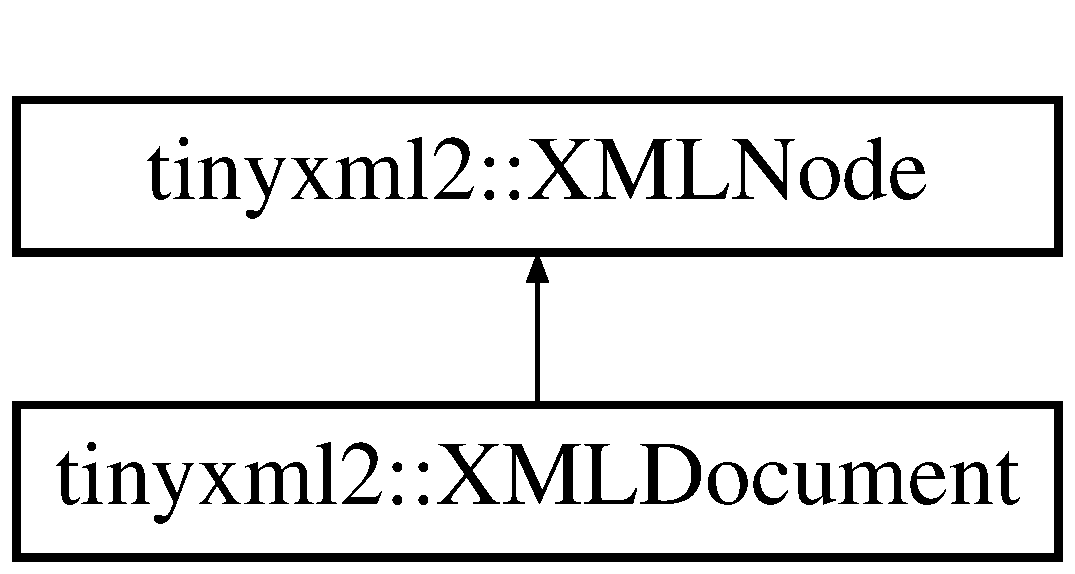
\includegraphics[height=2.000000cm]{classtinyxml2_1_1_x_m_l_document}
\end{center}
\end{figure}
\subsection*{Public Member Functions}
\begin{DoxyCompactItemize}
\item 
\hyperlink{classtinyxml2_1_1_x_m_l_document_af1574f76ebb619f25ef3f09eb2ba5188}{X\-M\-L\-Document} (bool process\-Entities=true, \hyperlink{namespacetinyxml2_a7f91d00f77360f850fd5da0861e27dd5}{Whitespace}=\hyperlink{namespacetinyxml2_a7f91d00f77360f850fd5da0861e27dd5a751769aa625fe5fe5286e9779edec56a}{P\-R\-E\-S\-E\-R\-V\-E\-\_\-\-W\-H\-I\-T\-E\-S\-P\-A\-C\-E})
\begin{DoxyCompactList}\small\item\em constructor \end{DoxyCompactList}\item 
\hyperlink{classtinyxml2_1_1_x_m_l_document_af37c47d8e2ba4b2fc81b21a77a32579b}{$\sim$\-X\-M\-L\-Document} ()
\item 
virtual \hyperlink{classtinyxml2_1_1_x_m_l_document}{X\-M\-L\-Document} $\ast$ \hyperlink{classtinyxml2_1_1_x_m_l_document_a3e185f880882bd978367bb55937735ec}{To\-Document} ()
\begin{DoxyCompactList}\small\item\em Safely cast to a Document, or null. \end{DoxyCompactList}\item 
virtual const \hyperlink{classtinyxml2_1_1_x_m_l_document}{X\-M\-L\-Document} $\ast$ \hyperlink{classtinyxml2_1_1_x_m_l_document_a15eb1a62afa18c66808031da647d1129}{To\-Document} () const 
\item 
\hyperlink{namespacetinyxml2_a1fbf88509c3ac88c09117b1947414e08}{X\-M\-L\-Error} \hyperlink{classtinyxml2_1_1_x_m_l_document_a1819bd34f540a7304c105a6232d25a1f}{Parse} (const char $\ast$xml, size\-\_\-t n\-Bytes=(size\-\_\-t)(-\/1))
\item 
\hyperlink{namespacetinyxml2_a1fbf88509c3ac88c09117b1947414e08}{X\-M\-L\-Error} \hyperlink{classtinyxml2_1_1_x_m_l_document_a2ebd4647a8af5fc6831b294ac26a150a}{Load\-File} (const char $\ast$filename)
\item 
\hyperlink{namespacetinyxml2_a1fbf88509c3ac88c09117b1947414e08}{X\-M\-L\-Error} \hyperlink{classtinyxml2_1_1_x_m_l_document_a5f1d330fad44c52f3d265338dd2a6dc2}{Load\-File} (F\-I\-L\-E $\ast$)
\item 
\hyperlink{namespacetinyxml2_a1fbf88509c3ac88c09117b1947414e08}{X\-M\-L\-Error} \hyperlink{classtinyxml2_1_1_x_m_l_document_a73ac416b4a2aa0952e841220eb3da18f}{Save\-File} (const char $\ast$filename, bool compact=false)
\item 
\hyperlink{namespacetinyxml2_a1fbf88509c3ac88c09117b1947414e08}{X\-M\-L\-Error} \hyperlink{classtinyxml2_1_1_x_m_l_document_a8b95779479a0035acc67b3a61dfe1b74}{Save\-File} (F\-I\-L\-E $\ast$fp, bool compact=false)
\item 
bool \hyperlink{classtinyxml2_1_1_x_m_l_document_adfcff7d0599cd520e9fcbb8891e1b678}{Process\-Entities} () const 
\item 
\hyperlink{namespacetinyxml2_a7f91d00f77360f850fd5da0861e27dd5}{Whitespace} \hyperlink{classtinyxml2_1_1_x_m_l_document_a94b3ea2f77c9ac831723984df5a02d01}{Whitespace\-Mode} () const 
\item 
bool \hyperlink{classtinyxml2_1_1_x_m_l_document_a530649e9de7e5aa8df9c37f66197fcb6}{Has\-B\-O\-M} () const 
\item 
void \hyperlink{classtinyxml2_1_1_x_m_l_document_a14419b698f7c4b140df4e80f3f0c93b0}{Set\-B\-O\-M} (bool use\-B\-O\-M)
\item 
\hyperlink{classtinyxml2_1_1_x_m_l_element}{X\-M\-L\-Element} $\ast$ \hyperlink{classtinyxml2_1_1_x_m_l_document_ad2b70320d3c2a071c2f36928edff3e1c}{Root\-Element} ()
\item 
const \hyperlink{classtinyxml2_1_1_x_m_l_element}{X\-M\-L\-Element} $\ast$ \hyperlink{classtinyxml2_1_1_x_m_l_document_a23a25b573d2adf3ee6075636c2a31c73}{Root\-Element} () const 
\item 
void \hyperlink{classtinyxml2_1_1_x_m_l_document_a686ea28672c0e0c60383ec28148c1ac0}{Print} (\hyperlink{classtinyxml2_1_1_x_m_l_printer}{X\-M\-L\-Printer} $\ast$streamer=0) const 
\item 
virtual bool \hyperlink{classtinyxml2_1_1_x_m_l_document_aa08503d24898bf9992ae5e5fb8b0cf87}{Accept} (\hyperlink{classtinyxml2_1_1_x_m_l_visitor}{X\-M\-L\-Visitor} $\ast$visitor) const 
\item 
\hyperlink{classtinyxml2_1_1_x_m_l_element}{X\-M\-L\-Element} $\ast$ \hyperlink{classtinyxml2_1_1_x_m_l_document_a3c335a700a43d7c363a393142a23f234}{New\-Element} (const char $\ast$name)
\item 
\hyperlink{classtinyxml2_1_1_x_m_l_comment}{X\-M\-L\-Comment} $\ast$ \hyperlink{classtinyxml2_1_1_x_m_l_document_a386df0befd06aadb5e0cd21381aa955a}{New\-Comment} (const char $\ast$comment)
\item 
\hyperlink{classtinyxml2_1_1_x_m_l_text}{X\-M\-L\-Text} $\ast$ \hyperlink{classtinyxml2_1_1_x_m_l_document_acece5de77a0819f2341b08c1e1ed9987}{New\-Text} (const char $\ast$text)
\item 
\hyperlink{classtinyxml2_1_1_x_m_l_declaration}{X\-M\-L\-Declaration} $\ast$ \hyperlink{classtinyxml2_1_1_x_m_l_document_ae519030c0262fa2daff8993681990e16}{New\-Declaration} (const char $\ast$text=0)
\item 
\hyperlink{classtinyxml2_1_1_x_m_l_unknown}{X\-M\-L\-Unknown} $\ast$ \hyperlink{classtinyxml2_1_1_x_m_l_document_a4954f502c5fd7f49de54c3c0c99bb73d}{New\-Unknown} (const char $\ast$text)
\item 
void \hyperlink{classtinyxml2_1_1_x_m_l_document_ac1d6e2c7fcc1a660624ac4f68e96380d}{Delete\-Node} (\hyperlink{classtinyxml2_1_1_x_m_l_node}{X\-M\-L\-Node} $\ast$node)
\item 
void \hyperlink{classtinyxml2_1_1_x_m_l_document_ae38d194e47336e4c96677ac77e2ac5d4}{Set\-Error} (\hyperlink{namespacetinyxml2_a1fbf88509c3ac88c09117b1947414e08}{X\-M\-L\-Error} error, const char $\ast$str1, const char $\ast$str2)
\item 
bool \hyperlink{classtinyxml2_1_1_x_m_l_document_abf0f9ac4c3aa5698a785937f71f7a69f}{Error} () const 
\begin{DoxyCompactList}\small\item\em Return true if there was an error parsing the document. \end{DoxyCompactList}\item 
\hyperlink{namespacetinyxml2_a1fbf88509c3ac88c09117b1947414e08}{X\-M\-L\-Error} \hyperlink{classtinyxml2_1_1_x_m_l_document_a34903418c9e83f27945c2c533839e350}{Error\-I\-D} () const 
\begin{DoxyCompactList}\small\item\em Return the error\-I\-D. \end{DoxyCompactList}\item 
const char $\ast$ \hyperlink{classtinyxml2_1_1_x_m_l_document_a016ccebecee36fe92084b5dfee6cc072}{Get\-Error\-Str1} () const 
\begin{DoxyCompactList}\small\item\em Return a possibly helpful diagnostic location or string. \end{DoxyCompactList}\item 
const char $\ast$ \hyperlink{classtinyxml2_1_1_x_m_l_document_a88f6b44bd019033bda28abd31fe257b2}{Get\-Error\-Str2} () const 
\begin{DoxyCompactList}\small\item\em Return a possibly helpful secondary diagnostic location or string. \end{DoxyCompactList}\item 
void \hyperlink{classtinyxml2_1_1_x_m_l_document_a7545cc9a9a67eee9307c001aa316a388}{Print\-Error} () const 
\begin{DoxyCompactList}\small\item\em If there is an error, print it to stdout. \end{DoxyCompactList}\item 
void \hyperlink{classtinyxml2_1_1_x_m_l_document_a65656b0b2cbc822708eb351504178aaf}{Clear} ()
\begin{DoxyCompactList}\small\item\em Clear the document, resetting it to the initial state. \end{DoxyCompactList}\item 
char $\ast$ \hyperlink{classtinyxml2_1_1_x_m_l_document_a25827d1bec509ad566a107e5853ed040}{Identify} (char $\ast$p, \hyperlink{classtinyxml2_1_1_x_m_l_node}{X\-M\-L\-Node} $\ast$$\ast$node)
\item 
virtual \hyperlink{classtinyxml2_1_1_x_m_l_node}{X\-M\-L\-Node} $\ast$ \hyperlink{classtinyxml2_1_1_x_m_l_document_a57c8511ed9f83aa3e20909a3db3f83d0}{Shallow\-Clone} (\hyperlink{classtinyxml2_1_1_x_m_l_document}{X\-M\-L\-Document} $\ast$) const 
\item 
virtual bool \hyperlink{classtinyxml2_1_1_x_m_l_document_a12eac66c6e45d074d5cc47319868cd66}{Shallow\-Equal} (const \hyperlink{classtinyxml2_1_1_x_m_l_node}{X\-M\-L\-Node} $\ast$) const 
\end{DoxyCompactItemize}
\subsection*{Private Member Functions}
\begin{DoxyCompactItemize}
\item 
\hyperlink{classtinyxml2_1_1_x_m_l_document_adcea490db02a099d99440cd14a87d9e4}{X\-M\-L\-Document} (const \hyperlink{classtinyxml2_1_1_x_m_l_document}{X\-M\-L\-Document} \&)
\item 
void \hyperlink{classtinyxml2_1_1_x_m_l_document_aa542c2cf1276ee4bd778f16d196fe222}{operator=} (const \hyperlink{classtinyxml2_1_1_x_m_l_document}{X\-M\-L\-Document} \&)
\end{DoxyCompactItemize}
\subsection*{Private Attributes}
\begin{DoxyCompactItemize}
\item 
bool \hyperlink{classtinyxml2_1_1_x_m_l_document_a1dbdc7feaa58007403c20243ac5abbd3}{\-\_\-write\-B\-O\-M}
\item 
bool \hyperlink{classtinyxml2_1_1_x_m_l_document_a9f768cb74fb5ccbadeffa436916f0194}{\-\_\-process\-Entities}
\item 
\hyperlink{namespacetinyxml2_a1fbf88509c3ac88c09117b1947414e08}{X\-M\-L\-Error} \hyperlink{classtinyxml2_1_1_x_m_l_document_a61270d643f810975656da2054e1e1622}{\-\_\-error\-I\-D}
\item 
\hyperlink{namespacetinyxml2_a7f91d00f77360f850fd5da0861e27dd5}{Whitespace} \hyperlink{classtinyxml2_1_1_x_m_l_document_a5342ed1e7dc1fe6afc81d4740c465320}{\-\_\-whitespace}
\item 
const char $\ast$ \hyperlink{classtinyxml2_1_1_x_m_l_document_a40948cedd3c1a0b19af0d483651e6aa8}{\-\_\-error\-Str1}
\item 
const char $\ast$ \hyperlink{classtinyxml2_1_1_x_m_l_document_a6627d1da446d48eefb03a86850e9bf6d}{\-\_\-error\-Str2}
\item 
char $\ast$ \hyperlink{classtinyxml2_1_1_x_m_l_document_a7913ff24220a40e2e2b49a5137b43d29}{\-\_\-char\-Buffer}
\item 
\hyperlink{classtinyxml2_1_1_mem_pool_t}{Mem\-Pool\-T}$<$ sizeof(\hyperlink{classtinyxml2_1_1_x_m_l_element}{X\-M\-L\-Element}) $>$ \hyperlink{classtinyxml2_1_1_x_m_l_document_a21574fba363a0d23bfc820d1652ab8bc}{\-\_\-element\-Pool}
\item 
\hyperlink{classtinyxml2_1_1_mem_pool_t}{Mem\-Pool\-T}$<$ sizeof(\hyperlink{classtinyxml2_1_1_x_m_l_attribute}{X\-M\-L\-Attribute}) $>$ \hyperlink{classtinyxml2_1_1_x_m_l_document_a0a57ebeba23bc6cfce88f12b4a946aac}{\-\_\-attribute\-Pool}
\item 
\hyperlink{classtinyxml2_1_1_mem_pool_t}{Mem\-Pool\-T}$<$ sizeof(\hyperlink{classtinyxml2_1_1_x_m_l_text}{X\-M\-L\-Text}) $>$ \hyperlink{classtinyxml2_1_1_x_m_l_document_afe8ac410aaa53cf1f2142a4c2fd958c7}{\-\_\-text\-Pool}
\item 
\hyperlink{classtinyxml2_1_1_mem_pool_t}{Mem\-Pool\-T}$<$ sizeof(\hyperlink{classtinyxml2_1_1_x_m_l_comment}{X\-M\-L\-Comment}) $>$ \hyperlink{classtinyxml2_1_1_x_m_l_document_ac2e73ccbc037dee917c3163158180398}{\-\_\-comment\-Pool}
\end{DoxyCompactItemize}
\subsection*{Friends}
\begin{DoxyCompactItemize}
\item 
class \hyperlink{classtinyxml2_1_1_x_m_l_document_ac2fba9b6e452829dd892f7392c24e0eb}{X\-M\-L\-Element}
\end{DoxyCompactItemize}
\subsection*{Additional Inherited Members}


\subsection{Detailed Description}
A Document binds together all the functionality. It can be saved, loaded, and printed to the screen. All Nodes are connected and allocated to a Document. If the Document is deleted, all its Nodes are also deleted. 

\subsection{Constructor \& Destructor Documentation}
\hypertarget{classtinyxml2_1_1_x_m_l_document_af1574f76ebb619f25ef3f09eb2ba5188}{\index{tinyxml2\-::\-X\-M\-L\-Document@{tinyxml2\-::\-X\-M\-L\-Document}!X\-M\-L\-Document@{X\-M\-L\-Document}}
\index{X\-M\-L\-Document@{X\-M\-L\-Document}!tinyxml2::XMLDocument@{tinyxml2\-::\-X\-M\-L\-Document}}
\subsubsection[{X\-M\-L\-Document}]{\setlength{\rightskip}{0pt plus 5cm}tinyxml2\-::\-X\-M\-L\-Document\-::\-X\-M\-L\-Document (
\begin{DoxyParamCaption}
\item[{bool}]{process\-Entities = {\ttfamily true}, }
\item[{{\bf Whitespace}}]{whitespace = {\ttfamily {\bf P\-R\-E\-S\-E\-R\-V\-E\-\_\-\-W\-H\-I\-T\-E\-S\-P\-A\-C\-E}}}
\end{DoxyParamCaption}
)}}\label{classtinyxml2_1_1_x_m_l_document_af1574f76ebb619f25ef3f09eb2ba5188}


constructor 

\hypertarget{classtinyxml2_1_1_x_m_l_document_af37c47d8e2ba4b2fc81b21a77a32579b}{\index{tinyxml2\-::\-X\-M\-L\-Document@{tinyxml2\-::\-X\-M\-L\-Document}!$\sim$\-X\-M\-L\-Document@{$\sim$\-X\-M\-L\-Document}}
\index{$\sim$\-X\-M\-L\-Document@{$\sim$\-X\-M\-L\-Document}!tinyxml2::XMLDocument@{tinyxml2\-::\-X\-M\-L\-Document}}
\subsubsection[{$\sim$\-X\-M\-L\-Document}]{\setlength{\rightskip}{0pt plus 5cm}tinyxml2\-::\-X\-M\-L\-Document\-::$\sim$\-X\-M\-L\-Document (
\begin{DoxyParamCaption}
{}
\end{DoxyParamCaption}
)}}\label{classtinyxml2_1_1_x_m_l_document_af37c47d8e2ba4b2fc81b21a77a32579b}
\hypertarget{classtinyxml2_1_1_x_m_l_document_adcea490db02a099d99440cd14a87d9e4}{\index{tinyxml2\-::\-X\-M\-L\-Document@{tinyxml2\-::\-X\-M\-L\-Document}!X\-M\-L\-Document@{X\-M\-L\-Document}}
\index{X\-M\-L\-Document@{X\-M\-L\-Document}!tinyxml2::XMLDocument@{tinyxml2\-::\-X\-M\-L\-Document}}
\subsubsection[{X\-M\-L\-Document}]{\setlength{\rightskip}{0pt plus 5cm}tinyxml2\-::\-X\-M\-L\-Document\-::\-X\-M\-L\-Document (
\begin{DoxyParamCaption}
\item[{const {\bf X\-M\-L\-Document} \&}]{}
\end{DoxyParamCaption}
)\hspace{0.3cm}{\ttfamily [private]}}}\label{classtinyxml2_1_1_x_m_l_document_adcea490db02a099d99440cd14a87d9e4}


\subsection{Member Function Documentation}
\hypertarget{classtinyxml2_1_1_x_m_l_document_aa08503d24898bf9992ae5e5fb8b0cf87}{\index{tinyxml2\-::\-X\-M\-L\-Document@{tinyxml2\-::\-X\-M\-L\-Document}!Accept@{Accept}}
\index{Accept@{Accept}!tinyxml2::XMLDocument@{tinyxml2\-::\-X\-M\-L\-Document}}
\subsubsection[{Accept}]{\setlength{\rightskip}{0pt plus 5cm}bool tinyxml2\-::\-X\-M\-L\-Document\-::\-Accept (
\begin{DoxyParamCaption}
\item[{{\bf X\-M\-L\-Visitor} $\ast$}]{visitor}
\end{DoxyParamCaption}
) const\hspace{0.3cm}{\ttfamily [virtual]}}}\label{classtinyxml2_1_1_x_m_l_document_aa08503d24898bf9992ae5e5fb8b0cf87}
Accept a hierarchical visit of the nodes in the Tiny\-X\-M\-L-\/2 D\-O\-M. Every node in the X\-M\-L tree will be conditionally visited and the host will be called back via the \hyperlink{classtinyxml2_1_1_x_m_l_visitor}{X\-M\-L\-Visitor} interface.

This is essentially a S\-A\-X interface for Tiny\-X\-M\-L-\/2. (Note however it doesn't re-\/parse the X\-M\-L for the callbacks, so the performance of Tiny\-X\-M\-L-\/2 is unchanged by using this interface versus any other.)

The interface has been based on ideas from\-:
\begin{DoxyItemize}
\item \href{http://www.saxproject.org/}{\tt http\-://www.\-saxproject.\-org/}
\item \href{http://c2.com/cgi/wiki?HierarchicalVisitorPattern}{\tt http\-://c2.\-com/cgi/wiki?\-Hierarchical\-Visitor\-Pattern}
\end{DoxyItemize}

Which are both good references for \char`\"{}visiting\char`\"{}.

An example of using \hyperlink{classtinyxml2_1_1_x_m_l_document_aa08503d24898bf9992ae5e5fb8b0cf87}{Accept()}\-: \begin{DoxyVerb}XMLPrinter printer;
tinyxmlDoc.Accept( &printer );
const char* xmlcstr = printer.CStr();
\end{DoxyVerb}
 

Implements \hyperlink{classtinyxml2_1_1_x_m_l_node_a81e66df0a44c67a7af17f3b77a152785}{tinyxml2\-::\-X\-M\-L\-Node}.

\hypertarget{classtinyxml2_1_1_x_m_l_document_a65656b0b2cbc822708eb351504178aaf}{\index{tinyxml2\-::\-X\-M\-L\-Document@{tinyxml2\-::\-X\-M\-L\-Document}!Clear@{Clear}}
\index{Clear@{Clear}!tinyxml2::XMLDocument@{tinyxml2\-::\-X\-M\-L\-Document}}
\subsubsection[{Clear}]{\setlength{\rightskip}{0pt plus 5cm}void tinyxml2\-::\-X\-M\-L\-Document\-::\-Clear (
\begin{DoxyParamCaption}
{}
\end{DoxyParamCaption}
)}}\label{classtinyxml2_1_1_x_m_l_document_a65656b0b2cbc822708eb351504178aaf}


Clear the document, resetting it to the initial state. 

\hypertarget{classtinyxml2_1_1_x_m_l_document_ac1d6e2c7fcc1a660624ac4f68e96380d}{\index{tinyxml2\-::\-X\-M\-L\-Document@{tinyxml2\-::\-X\-M\-L\-Document}!Delete\-Node@{Delete\-Node}}
\index{Delete\-Node@{Delete\-Node}!tinyxml2::XMLDocument@{tinyxml2\-::\-X\-M\-L\-Document}}
\subsubsection[{Delete\-Node}]{\setlength{\rightskip}{0pt plus 5cm}void tinyxml2\-::\-X\-M\-L\-Document\-::\-Delete\-Node (
\begin{DoxyParamCaption}
\item[{{\bf X\-M\-L\-Node} $\ast$}]{node}
\end{DoxyParamCaption}
)\hspace{0.3cm}{\ttfamily [inline]}}}\label{classtinyxml2_1_1_x_m_l_document_ac1d6e2c7fcc1a660624ac4f68e96380d}
Delete a node associated with this document. It will be unlinked from the D\-O\-M. \hypertarget{classtinyxml2_1_1_x_m_l_document_abf0f9ac4c3aa5698a785937f71f7a69f}{\index{tinyxml2\-::\-X\-M\-L\-Document@{tinyxml2\-::\-X\-M\-L\-Document}!Error@{Error}}
\index{Error@{Error}!tinyxml2::XMLDocument@{tinyxml2\-::\-X\-M\-L\-Document}}
\subsubsection[{Error}]{\setlength{\rightskip}{0pt plus 5cm}bool tinyxml2\-::\-X\-M\-L\-Document\-::\-Error (
\begin{DoxyParamCaption}
{}
\end{DoxyParamCaption}
) const\hspace{0.3cm}{\ttfamily [inline]}}}\label{classtinyxml2_1_1_x_m_l_document_abf0f9ac4c3aa5698a785937f71f7a69f}


Return true if there was an error parsing the document. 

\hypertarget{classtinyxml2_1_1_x_m_l_document_a34903418c9e83f27945c2c533839e350}{\index{tinyxml2\-::\-X\-M\-L\-Document@{tinyxml2\-::\-X\-M\-L\-Document}!Error\-I\-D@{Error\-I\-D}}
\index{Error\-I\-D@{Error\-I\-D}!tinyxml2::XMLDocument@{tinyxml2\-::\-X\-M\-L\-Document}}
\subsubsection[{Error\-I\-D}]{\setlength{\rightskip}{0pt plus 5cm}{\bf X\-M\-L\-Error} tinyxml2\-::\-X\-M\-L\-Document\-::\-Error\-I\-D (
\begin{DoxyParamCaption}
{}
\end{DoxyParamCaption}
) const\hspace{0.3cm}{\ttfamily [inline]}}}\label{classtinyxml2_1_1_x_m_l_document_a34903418c9e83f27945c2c533839e350}


Return the error\-I\-D. 

\hypertarget{classtinyxml2_1_1_x_m_l_document_a016ccebecee36fe92084b5dfee6cc072}{\index{tinyxml2\-::\-X\-M\-L\-Document@{tinyxml2\-::\-X\-M\-L\-Document}!Get\-Error\-Str1@{Get\-Error\-Str1}}
\index{Get\-Error\-Str1@{Get\-Error\-Str1}!tinyxml2::XMLDocument@{tinyxml2\-::\-X\-M\-L\-Document}}
\subsubsection[{Get\-Error\-Str1}]{\setlength{\rightskip}{0pt plus 5cm}const char$\ast$ tinyxml2\-::\-X\-M\-L\-Document\-::\-Get\-Error\-Str1 (
\begin{DoxyParamCaption}
{}
\end{DoxyParamCaption}
) const\hspace{0.3cm}{\ttfamily [inline]}}}\label{classtinyxml2_1_1_x_m_l_document_a016ccebecee36fe92084b5dfee6cc072}


Return a possibly helpful diagnostic location or string. 

\hypertarget{classtinyxml2_1_1_x_m_l_document_a88f6b44bd019033bda28abd31fe257b2}{\index{tinyxml2\-::\-X\-M\-L\-Document@{tinyxml2\-::\-X\-M\-L\-Document}!Get\-Error\-Str2@{Get\-Error\-Str2}}
\index{Get\-Error\-Str2@{Get\-Error\-Str2}!tinyxml2::XMLDocument@{tinyxml2\-::\-X\-M\-L\-Document}}
\subsubsection[{Get\-Error\-Str2}]{\setlength{\rightskip}{0pt plus 5cm}const char$\ast$ tinyxml2\-::\-X\-M\-L\-Document\-::\-Get\-Error\-Str2 (
\begin{DoxyParamCaption}
{}
\end{DoxyParamCaption}
) const\hspace{0.3cm}{\ttfamily [inline]}}}\label{classtinyxml2_1_1_x_m_l_document_a88f6b44bd019033bda28abd31fe257b2}


Return a possibly helpful secondary diagnostic location or string. 

\hypertarget{classtinyxml2_1_1_x_m_l_document_a530649e9de7e5aa8df9c37f66197fcb6}{\index{tinyxml2\-::\-X\-M\-L\-Document@{tinyxml2\-::\-X\-M\-L\-Document}!Has\-B\-O\-M@{Has\-B\-O\-M}}
\index{Has\-B\-O\-M@{Has\-B\-O\-M}!tinyxml2::XMLDocument@{tinyxml2\-::\-X\-M\-L\-Document}}
\subsubsection[{Has\-B\-O\-M}]{\setlength{\rightskip}{0pt plus 5cm}bool tinyxml2\-::\-X\-M\-L\-Document\-::\-Has\-B\-O\-M (
\begin{DoxyParamCaption}
{}
\end{DoxyParamCaption}
) const\hspace{0.3cm}{\ttfamily [inline]}}}\label{classtinyxml2_1_1_x_m_l_document_a530649e9de7e5aa8df9c37f66197fcb6}
Returns true if this document has a leading Byte Order Mark of U\-T\-F8. \hypertarget{classtinyxml2_1_1_x_m_l_document_a25827d1bec509ad566a107e5853ed040}{\index{tinyxml2\-::\-X\-M\-L\-Document@{tinyxml2\-::\-X\-M\-L\-Document}!Identify@{Identify}}
\index{Identify@{Identify}!tinyxml2::XMLDocument@{tinyxml2\-::\-X\-M\-L\-Document}}
\subsubsection[{Identify}]{\setlength{\rightskip}{0pt plus 5cm}char $\ast$ tinyxml2\-::\-X\-M\-L\-Document\-::\-Identify (
\begin{DoxyParamCaption}
\item[{char $\ast$}]{p, }
\item[{{\bf X\-M\-L\-Node} $\ast$$\ast$}]{node}
\end{DoxyParamCaption}
)}}\label{classtinyxml2_1_1_x_m_l_document_a25827d1bec509ad566a107e5853ed040}
\hypertarget{classtinyxml2_1_1_x_m_l_document_a2ebd4647a8af5fc6831b294ac26a150a}{\index{tinyxml2\-::\-X\-M\-L\-Document@{tinyxml2\-::\-X\-M\-L\-Document}!Load\-File@{Load\-File}}
\index{Load\-File@{Load\-File}!tinyxml2::XMLDocument@{tinyxml2\-::\-X\-M\-L\-Document}}
\subsubsection[{Load\-File}]{\setlength{\rightskip}{0pt plus 5cm}{\bf X\-M\-L\-Error} tinyxml2\-::\-X\-M\-L\-Document\-::\-Load\-File (
\begin{DoxyParamCaption}
\item[{const char $\ast$}]{filename}
\end{DoxyParamCaption}
)}}\label{classtinyxml2_1_1_x_m_l_document_a2ebd4647a8af5fc6831b294ac26a150a}
Load an X\-M\-L file from disk. Returns X\-M\-L\-\_\-\-N\-O\-\_\-\-E\-R\-R\-O\-R (0) on success, or an error\-I\-D. \hypertarget{classtinyxml2_1_1_x_m_l_document_a5f1d330fad44c52f3d265338dd2a6dc2}{\index{tinyxml2\-::\-X\-M\-L\-Document@{tinyxml2\-::\-X\-M\-L\-Document}!Load\-File@{Load\-File}}
\index{Load\-File@{Load\-File}!tinyxml2::XMLDocument@{tinyxml2\-::\-X\-M\-L\-Document}}
\subsubsection[{Load\-File}]{\setlength{\rightskip}{0pt plus 5cm}{\bf X\-M\-L\-Error} tinyxml2\-::\-X\-M\-L\-Document\-::\-Load\-File (
\begin{DoxyParamCaption}
\item[{F\-I\-L\-E $\ast$}]{fp}
\end{DoxyParamCaption}
)}}\label{classtinyxml2_1_1_x_m_l_document_a5f1d330fad44c52f3d265338dd2a6dc2}
Load an X\-M\-L file from disk. You are responsible for providing and closing the F\-I\-L\-E$\ast$.

Returns X\-M\-L\-\_\-\-N\-O\-\_\-\-E\-R\-R\-O\-R (0) on success, or an error\-I\-D. \hypertarget{classtinyxml2_1_1_x_m_l_document_a386df0befd06aadb5e0cd21381aa955a}{\index{tinyxml2\-::\-X\-M\-L\-Document@{tinyxml2\-::\-X\-M\-L\-Document}!New\-Comment@{New\-Comment}}
\index{New\-Comment@{New\-Comment}!tinyxml2::XMLDocument@{tinyxml2\-::\-X\-M\-L\-Document}}
\subsubsection[{New\-Comment}]{\setlength{\rightskip}{0pt plus 5cm}{\bf X\-M\-L\-Comment} $\ast$ tinyxml2\-::\-X\-M\-L\-Document\-::\-New\-Comment (
\begin{DoxyParamCaption}
\item[{const char $\ast$}]{comment}
\end{DoxyParamCaption}
)}}\label{classtinyxml2_1_1_x_m_l_document_a386df0befd06aadb5e0cd21381aa955a}
Create a new Comment associated with this Document. The memory for the Comment is managed by the Document. \hypertarget{classtinyxml2_1_1_x_m_l_document_ae519030c0262fa2daff8993681990e16}{\index{tinyxml2\-::\-X\-M\-L\-Document@{tinyxml2\-::\-X\-M\-L\-Document}!New\-Declaration@{New\-Declaration}}
\index{New\-Declaration@{New\-Declaration}!tinyxml2::XMLDocument@{tinyxml2\-::\-X\-M\-L\-Document}}
\subsubsection[{New\-Declaration}]{\setlength{\rightskip}{0pt plus 5cm}{\bf X\-M\-L\-Declaration} $\ast$ tinyxml2\-::\-X\-M\-L\-Document\-::\-New\-Declaration (
\begin{DoxyParamCaption}
\item[{const char $\ast$}]{text = {\ttfamily 0}}
\end{DoxyParamCaption}
)}}\label{classtinyxml2_1_1_x_m_l_document_ae519030c0262fa2daff8993681990e16}
Create a new Declaration associated with this Document. The memory for the object is managed by the Document.

If the 'text' param is null, the standard declaration is used.\-: \begin{DoxyVerb}    <?xml version="1.0" encoding="UTF-8"?>
\end{DoxyVerb}
 \hypertarget{classtinyxml2_1_1_x_m_l_document_a3c335a700a43d7c363a393142a23f234}{\index{tinyxml2\-::\-X\-M\-L\-Document@{tinyxml2\-::\-X\-M\-L\-Document}!New\-Element@{New\-Element}}
\index{New\-Element@{New\-Element}!tinyxml2::XMLDocument@{tinyxml2\-::\-X\-M\-L\-Document}}
\subsubsection[{New\-Element}]{\setlength{\rightskip}{0pt plus 5cm}{\bf X\-M\-L\-Element} $\ast$ tinyxml2\-::\-X\-M\-L\-Document\-::\-New\-Element (
\begin{DoxyParamCaption}
\item[{const char $\ast$}]{name}
\end{DoxyParamCaption}
)}}\label{classtinyxml2_1_1_x_m_l_document_a3c335a700a43d7c363a393142a23f234}
Create a new Element associated with this Document. The memory for the Element is managed by the Document. \hypertarget{classtinyxml2_1_1_x_m_l_document_acece5de77a0819f2341b08c1e1ed9987}{\index{tinyxml2\-::\-X\-M\-L\-Document@{tinyxml2\-::\-X\-M\-L\-Document}!New\-Text@{New\-Text}}
\index{New\-Text@{New\-Text}!tinyxml2::XMLDocument@{tinyxml2\-::\-X\-M\-L\-Document}}
\subsubsection[{New\-Text}]{\setlength{\rightskip}{0pt plus 5cm}{\bf X\-M\-L\-Text} $\ast$ tinyxml2\-::\-X\-M\-L\-Document\-::\-New\-Text (
\begin{DoxyParamCaption}
\item[{const char $\ast$}]{text}
\end{DoxyParamCaption}
)}}\label{classtinyxml2_1_1_x_m_l_document_acece5de77a0819f2341b08c1e1ed9987}
Create a new Text associated with this Document. The memory for the Text is managed by the Document. \hypertarget{classtinyxml2_1_1_x_m_l_document_a4954f502c5fd7f49de54c3c0c99bb73d}{\index{tinyxml2\-::\-X\-M\-L\-Document@{tinyxml2\-::\-X\-M\-L\-Document}!New\-Unknown@{New\-Unknown}}
\index{New\-Unknown@{New\-Unknown}!tinyxml2::XMLDocument@{tinyxml2\-::\-X\-M\-L\-Document}}
\subsubsection[{New\-Unknown}]{\setlength{\rightskip}{0pt plus 5cm}{\bf X\-M\-L\-Unknown} $\ast$ tinyxml2\-::\-X\-M\-L\-Document\-::\-New\-Unknown (
\begin{DoxyParamCaption}
\item[{const char $\ast$}]{text}
\end{DoxyParamCaption}
)}}\label{classtinyxml2_1_1_x_m_l_document_a4954f502c5fd7f49de54c3c0c99bb73d}
Create a new Unknown associated with this Document. The memory for the object is managed by the Document. \hypertarget{classtinyxml2_1_1_x_m_l_document_aa542c2cf1276ee4bd778f16d196fe222}{\index{tinyxml2\-::\-X\-M\-L\-Document@{tinyxml2\-::\-X\-M\-L\-Document}!operator=@{operator=}}
\index{operator=@{operator=}!tinyxml2::XMLDocument@{tinyxml2\-::\-X\-M\-L\-Document}}
\subsubsection[{operator=}]{\setlength{\rightskip}{0pt plus 5cm}void tinyxml2\-::\-X\-M\-L\-Document\-::operator= (
\begin{DoxyParamCaption}
\item[{const {\bf X\-M\-L\-Document} \&}]{}
\end{DoxyParamCaption}
)\hspace{0.3cm}{\ttfamily [private]}}}\label{classtinyxml2_1_1_x_m_l_document_aa542c2cf1276ee4bd778f16d196fe222}
\hypertarget{classtinyxml2_1_1_x_m_l_document_a1819bd34f540a7304c105a6232d25a1f}{\index{tinyxml2\-::\-X\-M\-L\-Document@{tinyxml2\-::\-X\-M\-L\-Document}!Parse@{Parse}}
\index{Parse@{Parse}!tinyxml2::XMLDocument@{tinyxml2\-::\-X\-M\-L\-Document}}
\subsubsection[{Parse}]{\setlength{\rightskip}{0pt plus 5cm}{\bf X\-M\-L\-Error} tinyxml2\-::\-X\-M\-L\-Document\-::\-Parse (
\begin{DoxyParamCaption}
\item[{const char $\ast$}]{xml, }
\item[{size\-\_\-t}]{n\-Bytes = {\ttfamily (size\-\_\-t)(-\/1)}}
\end{DoxyParamCaption}
)}}\label{classtinyxml2_1_1_x_m_l_document_a1819bd34f540a7304c105a6232d25a1f}
Parse an X\-M\-L file from a character string. Returns X\-M\-L\-\_\-\-N\-O\-\_\-\-E\-R\-R\-O\-R (0) on success, or an error\-I\-D.

You may optionally pass in the 'n\-Bytes', which is the number of bytes which will be parsed. If not specified, Tiny\-X\-M\-L-\/2 will assume 'xml' points to a null terminated string. \hypertarget{classtinyxml2_1_1_x_m_l_document_a686ea28672c0e0c60383ec28148c1ac0}{\index{tinyxml2\-::\-X\-M\-L\-Document@{tinyxml2\-::\-X\-M\-L\-Document}!Print@{Print}}
\index{Print@{Print}!tinyxml2::XMLDocument@{tinyxml2\-::\-X\-M\-L\-Document}}
\subsubsection[{Print}]{\setlength{\rightskip}{0pt plus 5cm}void tinyxml2\-::\-X\-M\-L\-Document\-::\-Print (
\begin{DoxyParamCaption}
\item[{{\bf X\-M\-L\-Printer} $\ast$}]{streamer = {\ttfamily 0}}
\end{DoxyParamCaption}
) const}}\label{classtinyxml2_1_1_x_m_l_document_a686ea28672c0e0c60383ec28148c1ac0}
Print the Document. If the Printer is not provided, it will print to stdout. If you provide Printer, this can print to a file\-: \begin{DoxyVerb}XMLPrinter printer( fp );
doc.Print( &printer );
\end{DoxyVerb}


Or you can use a printer to print to memory\-: \begin{DoxyVerb}XMLPrinter printer;
doc.Print( &printer );
// printer.CStr() has a const char* to the XML
\end{DoxyVerb}
 \hypertarget{classtinyxml2_1_1_x_m_l_document_a7545cc9a9a67eee9307c001aa316a388}{\index{tinyxml2\-::\-X\-M\-L\-Document@{tinyxml2\-::\-X\-M\-L\-Document}!Print\-Error@{Print\-Error}}
\index{Print\-Error@{Print\-Error}!tinyxml2::XMLDocument@{tinyxml2\-::\-X\-M\-L\-Document}}
\subsubsection[{Print\-Error}]{\setlength{\rightskip}{0pt plus 5cm}void tinyxml2\-::\-X\-M\-L\-Document\-::\-Print\-Error (
\begin{DoxyParamCaption}
{}
\end{DoxyParamCaption}
) const}}\label{classtinyxml2_1_1_x_m_l_document_a7545cc9a9a67eee9307c001aa316a388}


If there is an error, print it to stdout. 

\hypertarget{classtinyxml2_1_1_x_m_l_document_adfcff7d0599cd520e9fcbb8891e1b678}{\index{tinyxml2\-::\-X\-M\-L\-Document@{tinyxml2\-::\-X\-M\-L\-Document}!Process\-Entities@{Process\-Entities}}
\index{Process\-Entities@{Process\-Entities}!tinyxml2::XMLDocument@{tinyxml2\-::\-X\-M\-L\-Document}}
\subsubsection[{Process\-Entities}]{\setlength{\rightskip}{0pt plus 5cm}bool tinyxml2\-::\-X\-M\-L\-Document\-::\-Process\-Entities (
\begin{DoxyParamCaption}
{}
\end{DoxyParamCaption}
) const\hspace{0.3cm}{\ttfamily [inline]}}}\label{classtinyxml2_1_1_x_m_l_document_adfcff7d0599cd520e9fcbb8891e1b678}
\hypertarget{classtinyxml2_1_1_x_m_l_document_ad2b70320d3c2a071c2f36928edff3e1c}{\index{tinyxml2\-::\-X\-M\-L\-Document@{tinyxml2\-::\-X\-M\-L\-Document}!Root\-Element@{Root\-Element}}
\index{Root\-Element@{Root\-Element}!tinyxml2::XMLDocument@{tinyxml2\-::\-X\-M\-L\-Document}}
\subsubsection[{Root\-Element}]{\setlength{\rightskip}{0pt plus 5cm}{\bf X\-M\-L\-Element}$\ast$ tinyxml2\-::\-X\-M\-L\-Document\-::\-Root\-Element (
\begin{DoxyParamCaption}
{}
\end{DoxyParamCaption}
)\hspace{0.3cm}{\ttfamily [inline]}}}\label{classtinyxml2_1_1_x_m_l_document_ad2b70320d3c2a071c2f36928edff3e1c}
Return the root element of D\-O\-M. Equivalent to \hyperlink{classtinyxml2_1_1_x_m_l_node_a20f48e99b03e9c17487944f229bee130}{First\-Child\-Element()}. To get the first node, use \hyperlink{classtinyxml2_1_1_x_m_l_node_a2d6c70c475146b48bc93a7fafdeff5e0}{First\-Child()}. \hypertarget{classtinyxml2_1_1_x_m_l_document_a23a25b573d2adf3ee6075636c2a31c73}{\index{tinyxml2\-::\-X\-M\-L\-Document@{tinyxml2\-::\-X\-M\-L\-Document}!Root\-Element@{Root\-Element}}
\index{Root\-Element@{Root\-Element}!tinyxml2::XMLDocument@{tinyxml2\-::\-X\-M\-L\-Document}}
\subsubsection[{Root\-Element}]{\setlength{\rightskip}{0pt plus 5cm}const {\bf X\-M\-L\-Element}$\ast$ tinyxml2\-::\-X\-M\-L\-Document\-::\-Root\-Element (
\begin{DoxyParamCaption}
{}
\end{DoxyParamCaption}
) const\hspace{0.3cm}{\ttfamily [inline]}}}\label{classtinyxml2_1_1_x_m_l_document_a23a25b573d2adf3ee6075636c2a31c73}
\hypertarget{classtinyxml2_1_1_x_m_l_document_a73ac416b4a2aa0952e841220eb3da18f}{\index{tinyxml2\-::\-X\-M\-L\-Document@{tinyxml2\-::\-X\-M\-L\-Document}!Save\-File@{Save\-File}}
\index{Save\-File@{Save\-File}!tinyxml2::XMLDocument@{tinyxml2\-::\-X\-M\-L\-Document}}
\subsubsection[{Save\-File}]{\setlength{\rightskip}{0pt plus 5cm}{\bf X\-M\-L\-Error} tinyxml2\-::\-X\-M\-L\-Document\-::\-Save\-File (
\begin{DoxyParamCaption}
\item[{const char $\ast$}]{filename, }
\item[{bool}]{compact = {\ttfamily false}}
\end{DoxyParamCaption}
)}}\label{classtinyxml2_1_1_x_m_l_document_a73ac416b4a2aa0952e841220eb3da18f}
Save the X\-M\-L file to disk. Returns X\-M\-L\-\_\-\-N\-O\-\_\-\-E\-R\-R\-O\-R (0) on success, or an error\-I\-D. \hypertarget{classtinyxml2_1_1_x_m_l_document_a8b95779479a0035acc67b3a61dfe1b74}{\index{tinyxml2\-::\-X\-M\-L\-Document@{tinyxml2\-::\-X\-M\-L\-Document}!Save\-File@{Save\-File}}
\index{Save\-File@{Save\-File}!tinyxml2::XMLDocument@{tinyxml2\-::\-X\-M\-L\-Document}}
\subsubsection[{Save\-File}]{\setlength{\rightskip}{0pt plus 5cm}{\bf X\-M\-L\-Error} tinyxml2\-::\-X\-M\-L\-Document\-::\-Save\-File (
\begin{DoxyParamCaption}
\item[{F\-I\-L\-E $\ast$}]{fp, }
\item[{bool}]{compact = {\ttfamily false}}
\end{DoxyParamCaption}
)}}\label{classtinyxml2_1_1_x_m_l_document_a8b95779479a0035acc67b3a61dfe1b74}
Save the X\-M\-L file to disk. You are responsible for providing and closing the F\-I\-L\-E$\ast$.

Returns X\-M\-L\-\_\-\-N\-O\-\_\-\-E\-R\-R\-O\-R (0) on success, or an error\-I\-D. \hypertarget{classtinyxml2_1_1_x_m_l_document_a14419b698f7c4b140df4e80f3f0c93b0}{\index{tinyxml2\-::\-X\-M\-L\-Document@{tinyxml2\-::\-X\-M\-L\-Document}!Set\-B\-O\-M@{Set\-B\-O\-M}}
\index{Set\-B\-O\-M@{Set\-B\-O\-M}!tinyxml2::XMLDocument@{tinyxml2\-::\-X\-M\-L\-Document}}
\subsubsection[{Set\-B\-O\-M}]{\setlength{\rightskip}{0pt plus 5cm}void tinyxml2\-::\-X\-M\-L\-Document\-::\-Set\-B\-O\-M (
\begin{DoxyParamCaption}
\item[{bool}]{use\-B\-O\-M}
\end{DoxyParamCaption}
)\hspace{0.3cm}{\ttfamily [inline]}}}\label{classtinyxml2_1_1_x_m_l_document_a14419b698f7c4b140df4e80f3f0c93b0}
Sets whether to write the B\-O\-M when writing the file. \hypertarget{classtinyxml2_1_1_x_m_l_document_ae38d194e47336e4c96677ac77e2ac5d4}{\index{tinyxml2\-::\-X\-M\-L\-Document@{tinyxml2\-::\-X\-M\-L\-Document}!Set\-Error@{Set\-Error}}
\index{Set\-Error@{Set\-Error}!tinyxml2::XMLDocument@{tinyxml2\-::\-X\-M\-L\-Document}}
\subsubsection[{Set\-Error}]{\setlength{\rightskip}{0pt plus 5cm}void tinyxml2\-::\-X\-M\-L\-Document\-::\-Set\-Error (
\begin{DoxyParamCaption}
\item[{{\bf X\-M\-L\-Error}}]{error, }
\item[{const char $\ast$}]{str1, }
\item[{const char $\ast$}]{str2}
\end{DoxyParamCaption}
)}}\label{classtinyxml2_1_1_x_m_l_document_ae38d194e47336e4c96677ac77e2ac5d4}
\hypertarget{classtinyxml2_1_1_x_m_l_document_a57c8511ed9f83aa3e20909a3db3f83d0}{\index{tinyxml2\-::\-X\-M\-L\-Document@{tinyxml2\-::\-X\-M\-L\-Document}!Shallow\-Clone@{Shallow\-Clone}}
\index{Shallow\-Clone@{Shallow\-Clone}!tinyxml2::XMLDocument@{tinyxml2\-::\-X\-M\-L\-Document}}
\subsubsection[{Shallow\-Clone}]{\setlength{\rightskip}{0pt plus 5cm}virtual {\bf X\-M\-L\-Node}$\ast$ tinyxml2\-::\-X\-M\-L\-Document\-::\-Shallow\-Clone (
\begin{DoxyParamCaption}
\item[{{\bf X\-M\-L\-Document} $\ast$}]{document}
\end{DoxyParamCaption}
) const\hspace{0.3cm}{\ttfamily [inline]}, {\ttfamily [virtual]}}}\label{classtinyxml2_1_1_x_m_l_document_a57c8511ed9f83aa3e20909a3db3f83d0}
Make a copy of this node, but not its children. You may pass in a Document pointer that will be the owner of the new Node. If the 'document' is null, then the node returned will be allocated from the current Document. (this-\/$>$\hyperlink{classtinyxml2_1_1_x_m_l_node_af343d1ef0b45c0020e62d784d7e67a68}{Get\-Document()})

Note\-: if called on a \hyperlink{classtinyxml2_1_1_x_m_l_document}{X\-M\-L\-Document}, this will return null. 

Implements \hyperlink{classtinyxml2_1_1_x_m_l_node_a8402cbd3129d20e9e6024bbcc0531283}{tinyxml2\-::\-X\-M\-L\-Node}.

\hypertarget{classtinyxml2_1_1_x_m_l_document_a12eac66c6e45d074d5cc47319868cd66}{\index{tinyxml2\-::\-X\-M\-L\-Document@{tinyxml2\-::\-X\-M\-L\-Document}!Shallow\-Equal@{Shallow\-Equal}}
\index{Shallow\-Equal@{Shallow\-Equal}!tinyxml2::XMLDocument@{tinyxml2\-::\-X\-M\-L\-Document}}
\subsubsection[{Shallow\-Equal}]{\setlength{\rightskip}{0pt plus 5cm}virtual bool tinyxml2\-::\-X\-M\-L\-Document\-::\-Shallow\-Equal (
\begin{DoxyParamCaption}
\item[{const {\bf X\-M\-L\-Node} $\ast$}]{compare}
\end{DoxyParamCaption}
) const\hspace{0.3cm}{\ttfamily [inline]}, {\ttfamily [virtual]}}}\label{classtinyxml2_1_1_x_m_l_document_a12eac66c6e45d074d5cc47319868cd66}
Test if 2 nodes are the same, but don't test children. The 2 nodes do not need to be in the same Document.

Note\-: if called on a \hyperlink{classtinyxml2_1_1_x_m_l_document}{X\-M\-L\-Document}, this will return false. 

Implements \hyperlink{classtinyxml2_1_1_x_m_l_node_a7ce18b751c3ea09eac292dca264f9226}{tinyxml2\-::\-X\-M\-L\-Node}.

\hypertarget{classtinyxml2_1_1_x_m_l_document_a3e185f880882bd978367bb55937735ec}{\index{tinyxml2\-::\-X\-M\-L\-Document@{tinyxml2\-::\-X\-M\-L\-Document}!To\-Document@{To\-Document}}
\index{To\-Document@{To\-Document}!tinyxml2::XMLDocument@{tinyxml2\-::\-X\-M\-L\-Document}}
\subsubsection[{To\-Document}]{\setlength{\rightskip}{0pt plus 5cm}virtual {\bf X\-M\-L\-Document}$\ast$ tinyxml2\-::\-X\-M\-L\-Document\-::\-To\-Document (
\begin{DoxyParamCaption}
{}
\end{DoxyParamCaption}
)\hspace{0.3cm}{\ttfamily [inline]}, {\ttfamily [virtual]}}}\label{classtinyxml2_1_1_x_m_l_document_a3e185f880882bd978367bb55937735ec}


Safely cast to a Document, or null. 



Reimplemented from \hyperlink{classtinyxml2_1_1_x_m_l_node_a836e2966ed736fc3c94f70e12a2a3357}{tinyxml2\-::\-X\-M\-L\-Node}.

\hypertarget{classtinyxml2_1_1_x_m_l_document_a15eb1a62afa18c66808031da647d1129}{\index{tinyxml2\-::\-X\-M\-L\-Document@{tinyxml2\-::\-X\-M\-L\-Document}!To\-Document@{To\-Document}}
\index{To\-Document@{To\-Document}!tinyxml2::XMLDocument@{tinyxml2\-::\-X\-M\-L\-Document}}
\subsubsection[{To\-Document}]{\setlength{\rightskip}{0pt plus 5cm}virtual const {\bf X\-M\-L\-Document}$\ast$ tinyxml2\-::\-X\-M\-L\-Document\-::\-To\-Document (
\begin{DoxyParamCaption}
{}
\end{DoxyParamCaption}
) const\hspace{0.3cm}{\ttfamily [inline]}, {\ttfamily [virtual]}}}\label{classtinyxml2_1_1_x_m_l_document_a15eb1a62afa18c66808031da647d1129}


Reimplemented from \hyperlink{classtinyxml2_1_1_x_m_l_node_a3ff975733a17d6ced3539b45544c8bf6}{tinyxml2\-::\-X\-M\-L\-Node}.

\hypertarget{classtinyxml2_1_1_x_m_l_document_a94b3ea2f77c9ac831723984df5a02d01}{\index{tinyxml2\-::\-X\-M\-L\-Document@{tinyxml2\-::\-X\-M\-L\-Document}!Whitespace\-Mode@{Whitespace\-Mode}}
\index{Whitespace\-Mode@{Whitespace\-Mode}!tinyxml2::XMLDocument@{tinyxml2\-::\-X\-M\-L\-Document}}
\subsubsection[{Whitespace\-Mode}]{\setlength{\rightskip}{0pt plus 5cm}{\bf Whitespace} tinyxml2\-::\-X\-M\-L\-Document\-::\-Whitespace\-Mode (
\begin{DoxyParamCaption}
{}
\end{DoxyParamCaption}
) const\hspace{0.3cm}{\ttfamily [inline]}}}\label{classtinyxml2_1_1_x_m_l_document_a94b3ea2f77c9ac831723984df5a02d01}


\subsection{Friends And Related Function Documentation}
\hypertarget{classtinyxml2_1_1_x_m_l_document_ac2fba9b6e452829dd892f7392c24e0eb}{\index{tinyxml2\-::\-X\-M\-L\-Document@{tinyxml2\-::\-X\-M\-L\-Document}!X\-M\-L\-Element@{X\-M\-L\-Element}}
\index{X\-M\-L\-Element@{X\-M\-L\-Element}!tinyxml2::XMLDocument@{tinyxml2\-::\-X\-M\-L\-Document}}
\subsubsection[{X\-M\-L\-Element}]{\setlength{\rightskip}{0pt plus 5cm}friend class {\bf X\-M\-L\-Element}\hspace{0.3cm}{\ttfamily [friend]}}}\label{classtinyxml2_1_1_x_m_l_document_ac2fba9b6e452829dd892f7392c24e0eb}


\subsection{Member Data Documentation}
\hypertarget{classtinyxml2_1_1_x_m_l_document_a0a57ebeba23bc6cfce88f12b4a946aac}{\index{tinyxml2\-::\-X\-M\-L\-Document@{tinyxml2\-::\-X\-M\-L\-Document}!\-\_\-attribute\-Pool@{\-\_\-attribute\-Pool}}
\index{\-\_\-attribute\-Pool@{\-\_\-attribute\-Pool}!tinyxml2::XMLDocument@{tinyxml2\-::\-X\-M\-L\-Document}}
\subsubsection[{\-\_\-attribute\-Pool}]{\setlength{\rightskip}{0pt plus 5cm}{\bf Mem\-Pool\-T}$<$ sizeof({\bf X\-M\-L\-Attribute}) $>$ tinyxml2\-::\-X\-M\-L\-Document\-::\-\_\-attribute\-Pool\hspace{0.3cm}{\ttfamily [private]}}}\label{classtinyxml2_1_1_x_m_l_document_a0a57ebeba23bc6cfce88f12b4a946aac}
\hypertarget{classtinyxml2_1_1_x_m_l_document_a7913ff24220a40e2e2b49a5137b43d29}{\index{tinyxml2\-::\-X\-M\-L\-Document@{tinyxml2\-::\-X\-M\-L\-Document}!\-\_\-char\-Buffer@{\-\_\-char\-Buffer}}
\index{\-\_\-char\-Buffer@{\-\_\-char\-Buffer}!tinyxml2::XMLDocument@{tinyxml2\-::\-X\-M\-L\-Document}}
\subsubsection[{\-\_\-char\-Buffer}]{\setlength{\rightskip}{0pt plus 5cm}char$\ast$ tinyxml2\-::\-X\-M\-L\-Document\-::\-\_\-char\-Buffer\hspace{0.3cm}{\ttfamily [private]}}}\label{classtinyxml2_1_1_x_m_l_document_a7913ff24220a40e2e2b49a5137b43d29}
\hypertarget{classtinyxml2_1_1_x_m_l_document_ac2e73ccbc037dee917c3163158180398}{\index{tinyxml2\-::\-X\-M\-L\-Document@{tinyxml2\-::\-X\-M\-L\-Document}!\-\_\-comment\-Pool@{\-\_\-comment\-Pool}}
\index{\-\_\-comment\-Pool@{\-\_\-comment\-Pool}!tinyxml2::XMLDocument@{tinyxml2\-::\-X\-M\-L\-Document}}
\subsubsection[{\-\_\-comment\-Pool}]{\setlength{\rightskip}{0pt plus 5cm}{\bf Mem\-Pool\-T}$<$ sizeof({\bf X\-M\-L\-Comment}) $>$ tinyxml2\-::\-X\-M\-L\-Document\-::\-\_\-comment\-Pool\hspace{0.3cm}{\ttfamily [private]}}}\label{classtinyxml2_1_1_x_m_l_document_ac2e73ccbc037dee917c3163158180398}
\hypertarget{classtinyxml2_1_1_x_m_l_document_a21574fba363a0d23bfc820d1652ab8bc}{\index{tinyxml2\-::\-X\-M\-L\-Document@{tinyxml2\-::\-X\-M\-L\-Document}!\-\_\-element\-Pool@{\-\_\-element\-Pool}}
\index{\-\_\-element\-Pool@{\-\_\-element\-Pool}!tinyxml2::XMLDocument@{tinyxml2\-::\-X\-M\-L\-Document}}
\subsubsection[{\-\_\-element\-Pool}]{\setlength{\rightskip}{0pt plus 5cm}{\bf Mem\-Pool\-T}$<$ sizeof({\bf X\-M\-L\-Element}) $>$ tinyxml2\-::\-X\-M\-L\-Document\-::\-\_\-element\-Pool\hspace{0.3cm}{\ttfamily [private]}}}\label{classtinyxml2_1_1_x_m_l_document_a21574fba363a0d23bfc820d1652ab8bc}
\hypertarget{classtinyxml2_1_1_x_m_l_document_a61270d643f810975656da2054e1e1622}{\index{tinyxml2\-::\-X\-M\-L\-Document@{tinyxml2\-::\-X\-M\-L\-Document}!\-\_\-error\-I\-D@{\-\_\-error\-I\-D}}
\index{\-\_\-error\-I\-D@{\-\_\-error\-I\-D}!tinyxml2::XMLDocument@{tinyxml2\-::\-X\-M\-L\-Document}}
\subsubsection[{\-\_\-error\-I\-D}]{\setlength{\rightskip}{0pt plus 5cm}{\bf X\-M\-L\-Error} tinyxml2\-::\-X\-M\-L\-Document\-::\-\_\-error\-I\-D\hspace{0.3cm}{\ttfamily [private]}}}\label{classtinyxml2_1_1_x_m_l_document_a61270d643f810975656da2054e1e1622}
\hypertarget{classtinyxml2_1_1_x_m_l_document_a40948cedd3c1a0b19af0d483651e6aa8}{\index{tinyxml2\-::\-X\-M\-L\-Document@{tinyxml2\-::\-X\-M\-L\-Document}!\-\_\-error\-Str1@{\-\_\-error\-Str1}}
\index{\-\_\-error\-Str1@{\-\_\-error\-Str1}!tinyxml2::XMLDocument@{tinyxml2\-::\-X\-M\-L\-Document}}
\subsubsection[{\-\_\-error\-Str1}]{\setlength{\rightskip}{0pt plus 5cm}const char$\ast$ tinyxml2\-::\-X\-M\-L\-Document\-::\-\_\-error\-Str1\hspace{0.3cm}{\ttfamily [private]}}}\label{classtinyxml2_1_1_x_m_l_document_a40948cedd3c1a0b19af0d483651e6aa8}
\hypertarget{classtinyxml2_1_1_x_m_l_document_a6627d1da446d48eefb03a86850e9bf6d}{\index{tinyxml2\-::\-X\-M\-L\-Document@{tinyxml2\-::\-X\-M\-L\-Document}!\-\_\-error\-Str2@{\-\_\-error\-Str2}}
\index{\-\_\-error\-Str2@{\-\_\-error\-Str2}!tinyxml2::XMLDocument@{tinyxml2\-::\-X\-M\-L\-Document}}
\subsubsection[{\-\_\-error\-Str2}]{\setlength{\rightskip}{0pt plus 5cm}const char$\ast$ tinyxml2\-::\-X\-M\-L\-Document\-::\-\_\-error\-Str2\hspace{0.3cm}{\ttfamily [private]}}}\label{classtinyxml2_1_1_x_m_l_document_a6627d1da446d48eefb03a86850e9bf6d}
\hypertarget{classtinyxml2_1_1_x_m_l_document_a9f768cb74fb5ccbadeffa436916f0194}{\index{tinyxml2\-::\-X\-M\-L\-Document@{tinyxml2\-::\-X\-M\-L\-Document}!\-\_\-process\-Entities@{\-\_\-process\-Entities}}
\index{\-\_\-process\-Entities@{\-\_\-process\-Entities}!tinyxml2::XMLDocument@{tinyxml2\-::\-X\-M\-L\-Document}}
\subsubsection[{\-\_\-process\-Entities}]{\setlength{\rightskip}{0pt plus 5cm}bool tinyxml2\-::\-X\-M\-L\-Document\-::\-\_\-process\-Entities\hspace{0.3cm}{\ttfamily [private]}}}\label{classtinyxml2_1_1_x_m_l_document_a9f768cb74fb5ccbadeffa436916f0194}
\hypertarget{classtinyxml2_1_1_x_m_l_document_afe8ac410aaa53cf1f2142a4c2fd958c7}{\index{tinyxml2\-::\-X\-M\-L\-Document@{tinyxml2\-::\-X\-M\-L\-Document}!\-\_\-text\-Pool@{\-\_\-text\-Pool}}
\index{\-\_\-text\-Pool@{\-\_\-text\-Pool}!tinyxml2::XMLDocument@{tinyxml2\-::\-X\-M\-L\-Document}}
\subsubsection[{\-\_\-text\-Pool}]{\setlength{\rightskip}{0pt plus 5cm}{\bf Mem\-Pool\-T}$<$ sizeof({\bf X\-M\-L\-Text}) $>$ tinyxml2\-::\-X\-M\-L\-Document\-::\-\_\-text\-Pool\hspace{0.3cm}{\ttfamily [private]}}}\label{classtinyxml2_1_1_x_m_l_document_afe8ac410aaa53cf1f2142a4c2fd958c7}
\hypertarget{classtinyxml2_1_1_x_m_l_document_a5342ed1e7dc1fe6afc81d4740c465320}{\index{tinyxml2\-::\-X\-M\-L\-Document@{tinyxml2\-::\-X\-M\-L\-Document}!\-\_\-whitespace@{\-\_\-whitespace}}
\index{\-\_\-whitespace@{\-\_\-whitespace}!tinyxml2::XMLDocument@{tinyxml2\-::\-X\-M\-L\-Document}}
\subsubsection[{\-\_\-whitespace}]{\setlength{\rightskip}{0pt plus 5cm}{\bf Whitespace} tinyxml2\-::\-X\-M\-L\-Document\-::\-\_\-whitespace\hspace{0.3cm}{\ttfamily [private]}}}\label{classtinyxml2_1_1_x_m_l_document_a5342ed1e7dc1fe6afc81d4740c465320}
\hypertarget{classtinyxml2_1_1_x_m_l_document_a1dbdc7feaa58007403c20243ac5abbd3}{\index{tinyxml2\-::\-X\-M\-L\-Document@{tinyxml2\-::\-X\-M\-L\-Document}!\-\_\-write\-B\-O\-M@{\-\_\-write\-B\-O\-M}}
\index{\-\_\-write\-B\-O\-M@{\-\_\-write\-B\-O\-M}!tinyxml2::XMLDocument@{tinyxml2\-::\-X\-M\-L\-Document}}
\subsubsection[{\-\_\-write\-B\-O\-M}]{\setlength{\rightskip}{0pt plus 5cm}bool tinyxml2\-::\-X\-M\-L\-Document\-::\-\_\-write\-B\-O\-M\hspace{0.3cm}{\ttfamily [private]}}}\label{classtinyxml2_1_1_x_m_l_document_a1dbdc7feaa58007403c20243ac5abbd3}


The documentation for this class was generated from the following files\-:\begin{DoxyCompactItemize}
\item 
Utils/\-X\-M\-L\-\_\-\-Config/\hyperlink{tinyxml2_8h}{tinyxml2.\-h}\item 
Utils/\-X\-M\-L\-\_\-\-Config/\hyperlink{tinyxml2_8cpp}{tinyxml2.\-cpp}\end{DoxyCompactItemize}

\hypertarget{classtinyxml2_1_1_x_m_l_element}{\section{tinyxml2\-:\-:X\-M\-L\-Element Class Reference}
\label{classtinyxml2_1_1_x_m_l_element}\index{tinyxml2\-::\-X\-M\-L\-Element@{tinyxml2\-::\-X\-M\-L\-Element}}
}


{\ttfamily \#include $<$tinyxml2.\-h$>$}

Inheritance diagram for tinyxml2\-:\-:X\-M\-L\-Element\-:\begin{figure}[H]
\begin{center}
\leavevmode
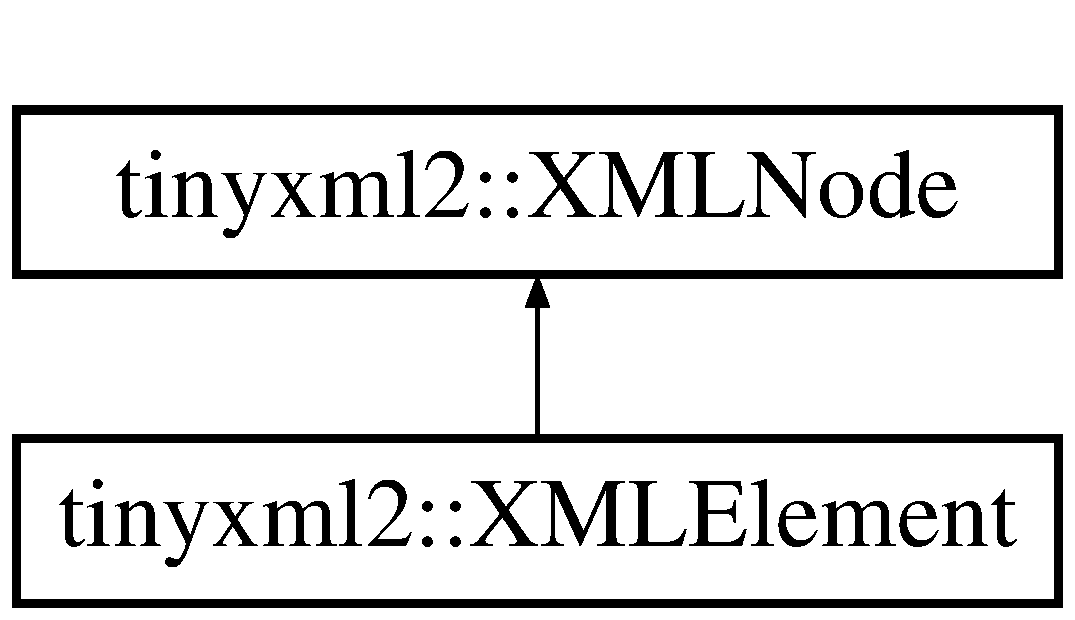
\includegraphics[height=2.000000cm]{classtinyxml2_1_1_x_m_l_element}
\end{center}
\end{figure}
\subsection*{Public Types}
\begin{DoxyCompactItemize}
\item 
enum \{ \hyperlink{classtinyxml2_1_1_x_m_l_element_a07a6ce25c17aaa505933db57f2373e50a78cf277c55b4655c86458dfecb11d349}{O\-P\-E\-N}, 
\hyperlink{classtinyxml2_1_1_x_m_l_element_a07a6ce25c17aaa505933db57f2373e50aa2f1f384020d2d4538ad2ec84930a028}{C\-L\-O\-S\-E\-D}, 
\hyperlink{classtinyxml2_1_1_x_m_l_element_a07a6ce25c17aaa505933db57f2373e50aa2857344b98a931536c443cd0cadc4b7}{C\-L\-O\-S\-I\-N\-G}
 \}
\end{DoxyCompactItemize}
\subsection*{Public Member Functions}
\begin{DoxyCompactItemize}
\item 
const char $\ast$ \hyperlink{classtinyxml2_1_1_x_m_l_element_a8bff355472bce2c60d4b50a212bf7f5f}{Name} () const 
\begin{DoxyCompactList}\small\item\em Get the name of an element (which is the \hyperlink{classtinyxml2_1_1_x_m_l_node_a92835c779871918f9af569bfe9669fe6}{Value()} of the node.) \end{DoxyCompactList}\item 
void \hyperlink{classtinyxml2_1_1_x_m_l_element_a97712009a530d8cb8a63bf705f02b4f1}{Set\-Name} (const char $\ast$str, bool static\-Mem=false)
\begin{DoxyCompactList}\small\item\em Set the name of the element. \end{DoxyCompactList}\item 
virtual \hyperlink{classtinyxml2_1_1_x_m_l_element}{X\-M\-L\-Element} $\ast$ \hyperlink{classtinyxml2_1_1_x_m_l_element_ad9ff5c2dbc15df36cf664ce1b0ea0a5d}{To\-Element} ()
\begin{DoxyCompactList}\small\item\em Safely cast to an Element, or null. \end{DoxyCompactList}\item 
virtual const \hyperlink{classtinyxml2_1_1_x_m_l_element}{X\-M\-L\-Element} $\ast$ \hyperlink{classtinyxml2_1_1_x_m_l_element_a55acab615353ddabab48271f95816b0d}{To\-Element} () const 
\item 
virtual bool \hyperlink{classtinyxml2_1_1_x_m_l_element_a36d65438991a1e85096caf39ad13a099}{Accept} (\hyperlink{classtinyxml2_1_1_x_m_l_visitor}{X\-M\-L\-Visitor} $\ast$visitor) const 
\item 
const char $\ast$ \hyperlink{classtinyxml2_1_1_x_m_l_element_a7bdebdf1888074087237f3dd03912740}{Attribute} (const char $\ast$name, const char $\ast$value=0) const 
\item 
int \hyperlink{classtinyxml2_1_1_x_m_l_element_af86f05771c11a73a2896b662bb589ef5}{Int\-Attribute} (const char $\ast$name) const 
\item 
unsigned \hyperlink{classtinyxml2_1_1_x_m_l_element_aa5a41367b5118acec42a87f5f94cec2d}{Unsigned\-Attribute} (const char $\ast$name) const 
\begin{DoxyCompactList}\small\item\em See \hyperlink{classtinyxml2_1_1_x_m_l_element_af86f05771c11a73a2896b662bb589ef5}{Int\-Attribute()} \end{DoxyCompactList}\item 
bool \hyperlink{classtinyxml2_1_1_x_m_l_element_a34811e4d1881e4ecc95c49f0f3799115}{Bool\-Attribute} (const char $\ast$name) const 
\begin{DoxyCompactList}\small\item\em See \hyperlink{classtinyxml2_1_1_x_m_l_element_af86f05771c11a73a2896b662bb589ef5}{Int\-Attribute()} \end{DoxyCompactList}\item 
double \hyperlink{classtinyxml2_1_1_x_m_l_element_a536922a5cae9c9769a3dc1b7a8ff0d44}{Double\-Attribute} (const char $\ast$name) const 
\begin{DoxyCompactList}\small\item\em See \hyperlink{classtinyxml2_1_1_x_m_l_element_af86f05771c11a73a2896b662bb589ef5}{Int\-Attribute()} \end{DoxyCompactList}\item 
float \hyperlink{classtinyxml2_1_1_x_m_l_element_a33b69f123f995aff966d2e351bc51b1f}{Float\-Attribute} (const char $\ast$name) const 
\begin{DoxyCompactList}\small\item\em See \hyperlink{classtinyxml2_1_1_x_m_l_element_af86f05771c11a73a2896b662bb589ef5}{Int\-Attribute()} \end{DoxyCompactList}\item 
\hyperlink{namespacetinyxml2_a1fbf88509c3ac88c09117b1947414e08}{X\-M\-L\-Error} \hyperlink{classtinyxml2_1_1_x_m_l_element_a8b92c729346aa8ea9acd59ed3e9f2378}{Query\-Int\-Attribute} (const char $\ast$name, int $\ast$value) const 
\item 
\hyperlink{namespacetinyxml2_a1fbf88509c3ac88c09117b1947414e08}{X\-M\-L\-Error} \hyperlink{classtinyxml2_1_1_x_m_l_element_aa3d8d1b9311da8fc249b4352749aaa84}{Query\-Unsigned\-Attribute} (const char $\ast$name, unsigned int $\ast$value) const 
\begin{DoxyCompactList}\small\item\em See \hyperlink{classtinyxml2_1_1_x_m_l_element_a8b92c729346aa8ea9acd59ed3e9f2378}{Query\-Int\-Attribute()} \end{DoxyCompactList}\item 
\hyperlink{namespacetinyxml2_a1fbf88509c3ac88c09117b1947414e08}{X\-M\-L\-Error} \hyperlink{classtinyxml2_1_1_x_m_l_element_a2a58ee941c3cda23772c887a8f8b534e}{Query\-Bool\-Attribute} (const char $\ast$name, bool $\ast$value) const 
\begin{DoxyCompactList}\small\item\em See \hyperlink{classtinyxml2_1_1_x_m_l_element_a8b92c729346aa8ea9acd59ed3e9f2378}{Query\-Int\-Attribute()} \end{DoxyCompactList}\item 
\hyperlink{namespacetinyxml2_a1fbf88509c3ac88c09117b1947414e08}{X\-M\-L\-Error} \hyperlink{classtinyxml2_1_1_x_m_l_element_a1ffeed461d3e4020b39652cd6d3cd773}{Query\-Double\-Attribute} (const char $\ast$name, double $\ast$value) const 
\begin{DoxyCompactList}\small\item\em See \hyperlink{classtinyxml2_1_1_x_m_l_element_a8b92c729346aa8ea9acd59ed3e9f2378}{Query\-Int\-Attribute()} \end{DoxyCompactList}\item 
\hyperlink{namespacetinyxml2_a1fbf88509c3ac88c09117b1947414e08}{X\-M\-L\-Error} \hyperlink{classtinyxml2_1_1_x_m_l_element_a3f154e0b4b6903249ff9f758921758e5}{Query\-Float\-Attribute} (const char $\ast$name, float $\ast$value) const 
\begin{DoxyCompactList}\small\item\em See \hyperlink{classtinyxml2_1_1_x_m_l_element_a8b92c729346aa8ea9acd59ed3e9f2378}{Query\-Int\-Attribute()} \end{DoxyCompactList}\item 
int \hyperlink{classtinyxml2_1_1_x_m_l_element_aa471a199af9f137ef371f5db1ed1016b}{Query\-Attribute} (const char $\ast$name, int $\ast$value) const 
\item 
int \hyperlink{classtinyxml2_1_1_x_m_l_element_a60d18656aa70adb257eab18913aa4330}{Query\-Attribute} (const char $\ast$name, unsigned int $\ast$value) const 
\item 
int \hyperlink{classtinyxml2_1_1_x_m_l_element_a23fa8bac4250249c476c6bfdb6cb9b9c}{Query\-Attribute} (const char $\ast$name, bool $\ast$value) const 
\item 
int \hyperlink{classtinyxml2_1_1_x_m_l_element_a64aadcbf27423410e2896baf240f63f9}{Query\-Attribute} (const char $\ast$name, double $\ast$value) const 
\item 
int \hyperlink{classtinyxml2_1_1_x_m_l_element_afd553774be0e7760d73003058efa8df9}{Query\-Attribute} (const char $\ast$name, float $\ast$value) const 
\item 
void \hyperlink{classtinyxml2_1_1_x_m_l_element_a11943abf2d0831548c3790dd5d9f119c}{Set\-Attribute} (const char $\ast$name, const char $\ast$value)
\begin{DoxyCompactList}\small\item\em Sets the named attribute to value. \end{DoxyCompactList}\item 
void \hyperlink{classtinyxml2_1_1_x_m_l_element_aae6568c64c7f1cc88be8461ba41a79cf}{Set\-Attribute} (const char $\ast$name, int value)
\begin{DoxyCompactList}\small\item\em Sets the named attribute to value. \end{DoxyCompactList}\item 
void \hyperlink{classtinyxml2_1_1_x_m_l_element_ae143997e90064ba82326b29a9930ea8f}{Set\-Attribute} (const char $\ast$name, unsigned value)
\begin{DoxyCompactList}\small\item\em Sets the named attribute to value. \end{DoxyCompactList}\item 
void \hyperlink{classtinyxml2_1_1_x_m_l_element_aa848b696e6a75e4e545c6da9893b11e1}{Set\-Attribute} (const char $\ast$name, bool value)
\begin{DoxyCompactList}\small\item\em Sets the named attribute to value. \end{DoxyCompactList}\item 
void \hyperlink{classtinyxml2_1_1_x_m_l_element_a233397ee81e70eb5d4b814c5f8698533}{Set\-Attribute} (const char $\ast$name, double value)
\begin{DoxyCompactList}\small\item\em Sets the named attribute to value. \end{DoxyCompactList}\item 
void \hyperlink{classtinyxml2_1_1_x_m_l_element_a554b70d882e65b28fc084b23df9b9759}{Set\-Attribute} (const char $\ast$name, float value)
\begin{DoxyCompactList}\small\item\em Sets the named attribute to value. \end{DoxyCompactList}\item 
void \hyperlink{classtinyxml2_1_1_x_m_l_element_aebd45aa7118964c30b32fe12e944628a}{Delete\-Attribute} (const char $\ast$name)
\item 
const \hyperlink{classtinyxml2_1_1_x_m_l_attribute}{X\-M\-L\-Attribute} $\ast$ \hyperlink{classtinyxml2_1_1_x_m_l_element_a67593e63558ffda0386699c3e4cc0b2c}{First\-Attribute} () const 
\begin{DoxyCompactList}\small\item\em Return the first attribute in the list. \end{DoxyCompactList}\item 
const \hyperlink{classtinyxml2_1_1_x_m_l_attribute}{X\-M\-L\-Attribute} $\ast$ \hyperlink{classtinyxml2_1_1_x_m_l_element_aaf46b0799ea419e5d070ac9a357de48f}{Find\-Attribute} (const char $\ast$name) const 
\begin{DoxyCompactList}\small\item\em Query a specific attribute in the list. \end{DoxyCompactList}\item 
const char $\ast$ \hyperlink{classtinyxml2_1_1_x_m_l_element_a56cc727044dad002b978256754d43a4b}{Get\-Text} () const 
\item 
void \hyperlink{classtinyxml2_1_1_x_m_l_element_a1f9c2cd61b72af5ae708d37b7ad283ce}{Set\-Text} (const char $\ast$in\-Text)
\item 
void \hyperlink{classtinyxml2_1_1_x_m_l_element_aeae8917b5ea6060b3c08d4e3d8d632d7}{Set\-Text} (int value)
\begin{DoxyCompactList}\small\item\em Convenience method for setting text inside and element. See \hyperlink{classtinyxml2_1_1_x_m_l_element_a1f9c2cd61b72af5ae708d37b7ad283ce}{Set\-Text()} for important limitations. \end{DoxyCompactList}\item 
void \hyperlink{classtinyxml2_1_1_x_m_l_element_a7bbfcc11d516598bc924a8fba4d08597}{Set\-Text} (unsigned value)
\begin{DoxyCompactList}\small\item\em Convenience method for setting text inside and element. See \hyperlink{classtinyxml2_1_1_x_m_l_element_a1f9c2cd61b72af5ae708d37b7ad283ce}{Set\-Text()} for important limitations. \end{DoxyCompactList}\item 
void \hyperlink{classtinyxml2_1_1_x_m_l_element_ae4b543d6770de76fb6ab68e541c192a4}{Set\-Text} (bool value)
\begin{DoxyCompactList}\small\item\em Convenience method for setting text inside and element. See \hyperlink{classtinyxml2_1_1_x_m_l_element_a1f9c2cd61b72af5ae708d37b7ad283ce}{Set\-Text()} for important limitations. \end{DoxyCompactList}\item 
void \hyperlink{classtinyxml2_1_1_x_m_l_element_a67bd77ac9aaeff58ff20b4275a65ba4e}{Set\-Text} (double value)
\begin{DoxyCompactList}\small\item\em Convenience method for setting text inside and element. See \hyperlink{classtinyxml2_1_1_x_m_l_element_a1f9c2cd61b72af5ae708d37b7ad283ce}{Set\-Text()} for important limitations. \end{DoxyCompactList}\item 
void \hyperlink{classtinyxml2_1_1_x_m_l_element_a51d560da5ae3ad6b75e0ab9ffb2ae42a}{Set\-Text} (float value)
\begin{DoxyCompactList}\small\item\em Convenience method for setting text inside and element. See \hyperlink{classtinyxml2_1_1_x_m_l_element_a1f9c2cd61b72af5ae708d37b7ad283ce}{Set\-Text()} for important limitations. \end{DoxyCompactList}\item 
\hyperlink{namespacetinyxml2_a1fbf88509c3ac88c09117b1947414e08}{X\-M\-L\-Error} \hyperlink{classtinyxml2_1_1_x_m_l_element_a71327c9a9d8840562bd204f46d0a7189}{Query\-Int\-Text} (int $\ast$ival) const 
\item 
\hyperlink{namespacetinyxml2_a1fbf88509c3ac88c09117b1947414e08}{X\-M\-L\-Error} \hyperlink{classtinyxml2_1_1_x_m_l_element_a2192091dec0c06be8b14f4e912c01758}{Query\-Unsigned\-Text} (unsigned $\ast$uval) const 
\begin{DoxyCompactList}\small\item\em See \hyperlink{classtinyxml2_1_1_x_m_l_element_a71327c9a9d8840562bd204f46d0a7189}{Query\-Int\-Text()} \end{DoxyCompactList}\item 
\hyperlink{namespacetinyxml2_a1fbf88509c3ac88c09117b1947414e08}{X\-M\-L\-Error} \hyperlink{classtinyxml2_1_1_x_m_l_element_afeb060672fa934163fc573e692b7fe38}{Query\-Bool\-Text} (bool $\ast$bval) const 
\begin{DoxyCompactList}\small\item\em See \hyperlink{classtinyxml2_1_1_x_m_l_element_a71327c9a9d8840562bd204f46d0a7189}{Query\-Int\-Text()} \end{DoxyCompactList}\item 
\hyperlink{namespacetinyxml2_a1fbf88509c3ac88c09117b1947414e08}{X\-M\-L\-Error} \hyperlink{classtinyxml2_1_1_x_m_l_element_aad931c42548907dbea416f7365d78b57}{Query\-Double\-Text} (double $\ast$dval) const 
\begin{DoxyCompactList}\small\item\em See \hyperlink{classtinyxml2_1_1_x_m_l_element_a71327c9a9d8840562bd204f46d0a7189}{Query\-Int\-Text()} \end{DoxyCompactList}\item 
\hyperlink{namespacetinyxml2_a1fbf88509c3ac88c09117b1947414e08}{X\-M\-L\-Error} \hyperlink{classtinyxml2_1_1_x_m_l_element_a11fa26e1dbca88e973964c1d9b597658}{Query\-Float\-Text} (float $\ast$fval) const 
\begin{DoxyCompactList}\small\item\em See \hyperlink{classtinyxml2_1_1_x_m_l_element_a71327c9a9d8840562bd204f46d0a7189}{Query\-Int\-Text()} \end{DoxyCompactList}\item 
int \hyperlink{classtinyxml2_1_1_x_m_l_element_a2e3d9f938307a05963d7c4b8cd55754e}{Closing\-Type} () const 
\item 
char $\ast$ \hyperlink{classtinyxml2_1_1_x_m_l_element_aaafdd2a5618abe80a2c1839ad3ccd492}{Parse\-Deep} (char $\ast$p, \hyperlink{classtinyxml2_1_1_str_pair}{Str\-Pair} $\ast$end\-Tag)
\item 
virtual \hyperlink{classtinyxml2_1_1_x_m_l_node}{X\-M\-L\-Node} $\ast$ \hyperlink{classtinyxml2_1_1_x_m_l_element_a85d85e32c18863fff1eeed53ae1ce23d}{Shallow\-Clone} (\hyperlink{classtinyxml2_1_1_x_m_l_document}{X\-M\-L\-Document} $\ast$document) const 
\item 
virtual bool \hyperlink{classtinyxml2_1_1_x_m_l_element_a25d51a2aad92625c78441457d58c85bc}{Shallow\-Equal} (const \hyperlink{classtinyxml2_1_1_x_m_l_node}{X\-M\-L\-Node} $\ast$compare) const 
\end{DoxyCompactItemize}
\subsection*{Private Types}
\begin{DoxyCompactItemize}
\item 
enum \{ \hyperlink{classtinyxml2_1_1_x_m_l_element_a80c7baddad73eb79786555f790687adaa21625cc023a5f905272d3f116cb9143e}{B\-U\-F\-\_\-\-S\-I\-Z\-E} = 200
 \}
\end{DoxyCompactItemize}
\subsection*{Private Member Functions}
\begin{DoxyCompactItemize}
\item 
\hyperlink{classtinyxml2_1_1_x_m_l_element_a52484940e20f3734e6edc5e5c3af2dbc}{X\-M\-L\-Element} (\hyperlink{classtinyxml2_1_1_x_m_l_document}{X\-M\-L\-Document} $\ast$doc)
\item 
virtual \hyperlink{classtinyxml2_1_1_x_m_l_element_a2b80613624153da83044a8b616fb325e}{$\sim$\-X\-M\-L\-Element} ()
\item 
\hyperlink{classtinyxml2_1_1_x_m_l_element_a1aa8ab977a1799bf118efb158248351b}{X\-M\-L\-Element} (const \hyperlink{classtinyxml2_1_1_x_m_l_element}{X\-M\-L\-Element} \&)
\item 
void \hyperlink{classtinyxml2_1_1_x_m_l_element_ae300366701a54d4b6d1c287d9b5209a7}{operator=} (const \hyperlink{classtinyxml2_1_1_x_m_l_element}{X\-M\-L\-Element} \&)
\item 
\hyperlink{classtinyxml2_1_1_x_m_l_attribute}{X\-M\-L\-Attribute} $\ast$ \hyperlink{classtinyxml2_1_1_x_m_l_element_a73cbfe2e24fd41c7d8544589312ef622}{Find\-Attribute} (const char $\ast$name)
\item 
\hyperlink{classtinyxml2_1_1_x_m_l_attribute}{X\-M\-L\-Attribute} $\ast$ \hyperlink{classtinyxml2_1_1_x_m_l_element_ac9d8fc849ec8acf46678217de011e896}{Find\-Or\-Create\-Attribute} (const char $\ast$name)
\item 
char $\ast$ \hyperlink{classtinyxml2_1_1_x_m_l_element_a9c931bc32d6e78b84c98f736fa8aafe2}{Parse\-Attributes} (char $\ast$p)
\end{DoxyCompactItemize}
\subsection*{Private Attributes}
\begin{DoxyCompactItemize}
\item 
int \hyperlink{classtinyxml2_1_1_x_m_l_element_ad6dbc2ecd157801ddc9bba7c3572796b}{\-\_\-closing\-Type}
\item 
\hyperlink{classtinyxml2_1_1_x_m_l_attribute}{X\-M\-L\-Attribute} $\ast$ \hyperlink{classtinyxml2_1_1_x_m_l_element_ad067115a9f42b2df1fcdf3e0355f2789}{\-\_\-root\-Attribute}
\end{DoxyCompactItemize}
\subsection*{Friends}
\begin{DoxyCompactItemize}
\item 
class \hyperlink{classtinyxml2_1_1_x_m_l_element_a449202cfc89e7ae5c2f81995476f9ec1}{X\-M\-L\-Base}
\item 
class \hyperlink{classtinyxml2_1_1_x_m_l_element_a4eee3bda60c60a30e4e8cd4ea91c4c6e}{X\-M\-L\-Document}
\end{DoxyCompactItemize}
\subsection*{Additional Inherited Members}


\subsection{Detailed Description}
The element is a container class. It has a value, the element name, and can contain other elements, text, comments, and unknowns. Elements also contain an arbitrary number of attributes. 

\subsection{Member Enumeration Documentation}
\hypertarget{classtinyxml2_1_1_x_m_l_element_a07a6ce25c17aaa505933db57f2373e50}{\subsubsection[{anonymous enum}]{\setlength{\rightskip}{0pt plus 5cm}anonymous enum}}\label{classtinyxml2_1_1_x_m_l_element_a07a6ce25c17aaa505933db57f2373e50}
\begin{Desc}
\item[Enumerator]\par
\begin{description}
\index{O\-P\-E\-N@{O\-P\-E\-N}!tinyxml2\-::\-X\-M\-L\-Element@{tinyxml2\-::\-X\-M\-L\-Element}}\index{tinyxml2\-::\-X\-M\-L\-Element@{tinyxml2\-::\-X\-M\-L\-Element}!O\-P\-E\-N@{O\-P\-E\-N}}\item[{\em 
\hypertarget{classtinyxml2_1_1_x_m_l_element_a07a6ce25c17aaa505933db57f2373e50a78cf277c55b4655c86458dfecb11d349}{O\-P\-E\-N}\label{classtinyxml2_1_1_x_m_l_element_a07a6ce25c17aaa505933db57f2373e50a78cf277c55b4655c86458dfecb11d349}
}]\index{C\-L\-O\-S\-E\-D@{C\-L\-O\-S\-E\-D}!tinyxml2\-::\-X\-M\-L\-Element@{tinyxml2\-::\-X\-M\-L\-Element}}\index{tinyxml2\-::\-X\-M\-L\-Element@{tinyxml2\-::\-X\-M\-L\-Element}!C\-L\-O\-S\-E\-D@{C\-L\-O\-S\-E\-D}}\item[{\em 
\hypertarget{classtinyxml2_1_1_x_m_l_element_a07a6ce25c17aaa505933db57f2373e50aa2f1f384020d2d4538ad2ec84930a028}{C\-L\-O\-S\-E\-D}\label{classtinyxml2_1_1_x_m_l_element_a07a6ce25c17aaa505933db57f2373e50aa2f1f384020d2d4538ad2ec84930a028}
}]\index{C\-L\-O\-S\-I\-N\-G@{C\-L\-O\-S\-I\-N\-G}!tinyxml2\-::\-X\-M\-L\-Element@{tinyxml2\-::\-X\-M\-L\-Element}}\index{tinyxml2\-::\-X\-M\-L\-Element@{tinyxml2\-::\-X\-M\-L\-Element}!C\-L\-O\-S\-I\-N\-G@{C\-L\-O\-S\-I\-N\-G}}\item[{\em 
\hypertarget{classtinyxml2_1_1_x_m_l_element_a07a6ce25c17aaa505933db57f2373e50aa2857344b98a931536c443cd0cadc4b7}{C\-L\-O\-S\-I\-N\-G}\label{classtinyxml2_1_1_x_m_l_element_a07a6ce25c17aaa505933db57f2373e50aa2857344b98a931536c443cd0cadc4b7}
}]\end{description}
\end{Desc}
\hypertarget{classtinyxml2_1_1_x_m_l_element_a80c7baddad73eb79786555f790687ada}{\subsubsection[{anonymous enum}]{\setlength{\rightskip}{0pt plus 5cm}anonymous enum\hspace{0.3cm}{\ttfamily [private]}}}\label{classtinyxml2_1_1_x_m_l_element_a80c7baddad73eb79786555f790687ada}
\begin{Desc}
\item[Enumerator]\par
\begin{description}
\index{B\-U\-F\-\_\-\-S\-I\-Z\-E@{B\-U\-F\-\_\-\-S\-I\-Z\-E}!tinyxml2\-::\-X\-M\-L\-Element@{tinyxml2\-::\-X\-M\-L\-Element}}\index{tinyxml2\-::\-X\-M\-L\-Element@{tinyxml2\-::\-X\-M\-L\-Element}!B\-U\-F\-\_\-\-S\-I\-Z\-E@{B\-U\-F\-\_\-\-S\-I\-Z\-E}}\item[{\em 
\hypertarget{classtinyxml2_1_1_x_m_l_element_a80c7baddad73eb79786555f790687adaa21625cc023a5f905272d3f116cb9143e}{B\-U\-F\-\_\-\-S\-I\-Z\-E}\label{classtinyxml2_1_1_x_m_l_element_a80c7baddad73eb79786555f790687adaa21625cc023a5f905272d3f116cb9143e}
}]\end{description}
\end{Desc}


\subsection{Constructor \& Destructor Documentation}
\hypertarget{classtinyxml2_1_1_x_m_l_element_a52484940e20f3734e6edc5e5c3af2dbc}{\index{tinyxml2\-::\-X\-M\-L\-Element@{tinyxml2\-::\-X\-M\-L\-Element}!X\-M\-L\-Element@{X\-M\-L\-Element}}
\index{X\-M\-L\-Element@{X\-M\-L\-Element}!tinyxml2::XMLElement@{tinyxml2\-::\-X\-M\-L\-Element}}
\subsubsection[{X\-M\-L\-Element}]{\setlength{\rightskip}{0pt plus 5cm}tinyxml2\-::\-X\-M\-L\-Element\-::\-X\-M\-L\-Element (
\begin{DoxyParamCaption}
\item[{{\bf X\-M\-L\-Document} $\ast$}]{doc}
\end{DoxyParamCaption}
)\hspace{0.3cm}{\ttfamily [private]}}}\label{classtinyxml2_1_1_x_m_l_element_a52484940e20f3734e6edc5e5c3af2dbc}
\hypertarget{classtinyxml2_1_1_x_m_l_element_a2b80613624153da83044a8b616fb325e}{\index{tinyxml2\-::\-X\-M\-L\-Element@{tinyxml2\-::\-X\-M\-L\-Element}!$\sim$\-X\-M\-L\-Element@{$\sim$\-X\-M\-L\-Element}}
\index{$\sim$\-X\-M\-L\-Element@{$\sim$\-X\-M\-L\-Element}!tinyxml2::XMLElement@{tinyxml2\-::\-X\-M\-L\-Element}}
\subsubsection[{$\sim$\-X\-M\-L\-Element}]{\setlength{\rightskip}{0pt plus 5cm}tinyxml2\-::\-X\-M\-L\-Element\-::$\sim$\-X\-M\-L\-Element (
\begin{DoxyParamCaption}
{}
\end{DoxyParamCaption}
)\hspace{0.3cm}{\ttfamily [private]}, {\ttfamily [virtual]}}}\label{classtinyxml2_1_1_x_m_l_element_a2b80613624153da83044a8b616fb325e}
\hypertarget{classtinyxml2_1_1_x_m_l_element_a1aa8ab977a1799bf118efb158248351b}{\index{tinyxml2\-::\-X\-M\-L\-Element@{tinyxml2\-::\-X\-M\-L\-Element}!X\-M\-L\-Element@{X\-M\-L\-Element}}
\index{X\-M\-L\-Element@{X\-M\-L\-Element}!tinyxml2::XMLElement@{tinyxml2\-::\-X\-M\-L\-Element}}
\subsubsection[{X\-M\-L\-Element}]{\setlength{\rightskip}{0pt plus 5cm}tinyxml2\-::\-X\-M\-L\-Element\-::\-X\-M\-L\-Element (
\begin{DoxyParamCaption}
\item[{const {\bf X\-M\-L\-Element} \&}]{}
\end{DoxyParamCaption}
)\hspace{0.3cm}{\ttfamily [private]}}}\label{classtinyxml2_1_1_x_m_l_element_a1aa8ab977a1799bf118efb158248351b}


\subsection{Member Function Documentation}
\hypertarget{classtinyxml2_1_1_x_m_l_element_a36d65438991a1e85096caf39ad13a099}{\index{tinyxml2\-::\-X\-M\-L\-Element@{tinyxml2\-::\-X\-M\-L\-Element}!Accept@{Accept}}
\index{Accept@{Accept}!tinyxml2::XMLElement@{tinyxml2\-::\-X\-M\-L\-Element}}
\subsubsection[{Accept}]{\setlength{\rightskip}{0pt plus 5cm}bool tinyxml2\-::\-X\-M\-L\-Element\-::\-Accept (
\begin{DoxyParamCaption}
\item[{{\bf X\-M\-L\-Visitor} $\ast$}]{visitor}
\end{DoxyParamCaption}
) const\hspace{0.3cm}{\ttfamily [virtual]}}}\label{classtinyxml2_1_1_x_m_l_element_a36d65438991a1e85096caf39ad13a099}
Accept a hierarchical visit of the nodes in the Tiny\-X\-M\-L-\/2 D\-O\-M. Every node in the X\-M\-L tree will be conditionally visited and the host will be called back via the \hyperlink{classtinyxml2_1_1_x_m_l_visitor}{X\-M\-L\-Visitor} interface.

This is essentially a S\-A\-X interface for Tiny\-X\-M\-L-\/2. (Note however it doesn't re-\/parse the X\-M\-L for the callbacks, so the performance of Tiny\-X\-M\-L-\/2 is unchanged by using this interface versus any other.)

The interface has been based on ideas from\-:
\begin{DoxyItemize}
\item \href{http://www.saxproject.org/}{\tt http\-://www.\-saxproject.\-org/}
\item \href{http://c2.com/cgi/wiki?HierarchicalVisitorPattern}{\tt http\-://c2.\-com/cgi/wiki?\-Hierarchical\-Visitor\-Pattern}
\end{DoxyItemize}

Which are both good references for \char`\"{}visiting\char`\"{}.

An example of using \hyperlink{classtinyxml2_1_1_x_m_l_element_a36d65438991a1e85096caf39ad13a099}{Accept()}\-: \begin{DoxyVerb}XMLPrinter printer;
tinyxmlDoc.Accept( &printer );
const char* xmlcstr = printer.CStr();
\end{DoxyVerb}
 

Implements \hyperlink{classtinyxml2_1_1_x_m_l_node_a81e66df0a44c67a7af17f3b77a152785}{tinyxml2\-::\-X\-M\-L\-Node}.

\hypertarget{classtinyxml2_1_1_x_m_l_element_a7bdebdf1888074087237f3dd03912740}{\index{tinyxml2\-::\-X\-M\-L\-Element@{tinyxml2\-::\-X\-M\-L\-Element}!Attribute@{Attribute}}
\index{Attribute@{Attribute}!tinyxml2::XMLElement@{tinyxml2\-::\-X\-M\-L\-Element}}
\subsubsection[{Attribute}]{\setlength{\rightskip}{0pt plus 5cm}const char $\ast$ tinyxml2\-::\-X\-M\-L\-Element\-::\-Attribute (
\begin{DoxyParamCaption}
\item[{const char $\ast$}]{name, }
\item[{const char $\ast$}]{value = {\ttfamily 0}}
\end{DoxyParamCaption}
) const}}\label{classtinyxml2_1_1_x_m_l_element_a7bdebdf1888074087237f3dd03912740}
Given an attribute name, \hyperlink{classtinyxml2_1_1_x_m_l_element_a7bdebdf1888074087237f3dd03912740}{Attribute()} returns the value for the attribute of that name, or null if none exists. For example\-:

\begin{DoxyVerb}const char* value = ele->Attribute( "foo" );
\end{DoxyVerb}


The 'value' parameter is normally null. However, if specified, the attribute will only be returned if the 'name' and 'value' match. This allow you to write code\-:

\begin{DoxyVerb}if ( ele->Attribute( "foo", "bar" ) ) callFooIsBar();
\end{DoxyVerb}


rather than\-: \begin{DoxyVerb}if ( ele->Attribute( "foo" ) ) {
    if ( strcmp( ele->Attribute( "foo" ), "bar" ) == 0 ) callFooIsBar();
}
\end{DoxyVerb}
 \hypertarget{classtinyxml2_1_1_x_m_l_element_a34811e4d1881e4ecc95c49f0f3799115}{\index{tinyxml2\-::\-X\-M\-L\-Element@{tinyxml2\-::\-X\-M\-L\-Element}!Bool\-Attribute@{Bool\-Attribute}}
\index{Bool\-Attribute@{Bool\-Attribute}!tinyxml2::XMLElement@{tinyxml2\-::\-X\-M\-L\-Element}}
\subsubsection[{Bool\-Attribute}]{\setlength{\rightskip}{0pt plus 5cm}bool tinyxml2\-::\-X\-M\-L\-Element\-::\-Bool\-Attribute (
\begin{DoxyParamCaption}
\item[{const char $\ast$}]{name}
\end{DoxyParamCaption}
) const\hspace{0.3cm}{\ttfamily [inline]}}}\label{classtinyxml2_1_1_x_m_l_element_a34811e4d1881e4ecc95c49f0f3799115}


See \hyperlink{classtinyxml2_1_1_x_m_l_element_af86f05771c11a73a2896b662bb589ef5}{Int\-Attribute()} 

\hypertarget{classtinyxml2_1_1_x_m_l_element_a2e3d9f938307a05963d7c4b8cd55754e}{\index{tinyxml2\-::\-X\-M\-L\-Element@{tinyxml2\-::\-X\-M\-L\-Element}!Closing\-Type@{Closing\-Type}}
\index{Closing\-Type@{Closing\-Type}!tinyxml2::XMLElement@{tinyxml2\-::\-X\-M\-L\-Element}}
\subsubsection[{Closing\-Type}]{\setlength{\rightskip}{0pt plus 5cm}int tinyxml2\-::\-X\-M\-L\-Element\-::\-Closing\-Type (
\begin{DoxyParamCaption}
{}
\end{DoxyParamCaption}
) const\hspace{0.3cm}{\ttfamily [inline]}}}\label{classtinyxml2_1_1_x_m_l_element_a2e3d9f938307a05963d7c4b8cd55754e}
\hypertarget{classtinyxml2_1_1_x_m_l_element_aebd45aa7118964c30b32fe12e944628a}{\index{tinyxml2\-::\-X\-M\-L\-Element@{tinyxml2\-::\-X\-M\-L\-Element}!Delete\-Attribute@{Delete\-Attribute}}
\index{Delete\-Attribute@{Delete\-Attribute}!tinyxml2::XMLElement@{tinyxml2\-::\-X\-M\-L\-Element}}
\subsubsection[{Delete\-Attribute}]{\setlength{\rightskip}{0pt plus 5cm}void tinyxml2\-::\-X\-M\-L\-Element\-::\-Delete\-Attribute (
\begin{DoxyParamCaption}
\item[{const char $\ast$}]{name}
\end{DoxyParamCaption}
)}}\label{classtinyxml2_1_1_x_m_l_element_aebd45aa7118964c30b32fe12e944628a}
Delete an attribute. \hypertarget{classtinyxml2_1_1_x_m_l_element_a536922a5cae9c9769a3dc1b7a8ff0d44}{\index{tinyxml2\-::\-X\-M\-L\-Element@{tinyxml2\-::\-X\-M\-L\-Element}!Double\-Attribute@{Double\-Attribute}}
\index{Double\-Attribute@{Double\-Attribute}!tinyxml2::XMLElement@{tinyxml2\-::\-X\-M\-L\-Element}}
\subsubsection[{Double\-Attribute}]{\setlength{\rightskip}{0pt plus 5cm}double tinyxml2\-::\-X\-M\-L\-Element\-::\-Double\-Attribute (
\begin{DoxyParamCaption}
\item[{const char $\ast$}]{name}
\end{DoxyParamCaption}
) const\hspace{0.3cm}{\ttfamily [inline]}}}\label{classtinyxml2_1_1_x_m_l_element_a536922a5cae9c9769a3dc1b7a8ff0d44}


See \hyperlink{classtinyxml2_1_1_x_m_l_element_af86f05771c11a73a2896b662bb589ef5}{Int\-Attribute()} 

\hypertarget{classtinyxml2_1_1_x_m_l_element_aaf46b0799ea419e5d070ac9a357de48f}{\index{tinyxml2\-::\-X\-M\-L\-Element@{tinyxml2\-::\-X\-M\-L\-Element}!Find\-Attribute@{Find\-Attribute}}
\index{Find\-Attribute@{Find\-Attribute}!tinyxml2::XMLElement@{tinyxml2\-::\-X\-M\-L\-Element}}
\subsubsection[{Find\-Attribute}]{\setlength{\rightskip}{0pt plus 5cm}const {\bf X\-M\-L\-Attribute} $\ast$ tinyxml2\-::\-X\-M\-L\-Element\-::\-Find\-Attribute (
\begin{DoxyParamCaption}
\item[{const char $\ast$}]{name}
\end{DoxyParamCaption}
) const}}\label{classtinyxml2_1_1_x_m_l_element_aaf46b0799ea419e5d070ac9a357de48f}


Query a specific attribute in the list. 

\hypertarget{classtinyxml2_1_1_x_m_l_element_a73cbfe2e24fd41c7d8544589312ef622}{\index{tinyxml2\-::\-X\-M\-L\-Element@{tinyxml2\-::\-X\-M\-L\-Element}!Find\-Attribute@{Find\-Attribute}}
\index{Find\-Attribute@{Find\-Attribute}!tinyxml2::XMLElement@{tinyxml2\-::\-X\-M\-L\-Element}}
\subsubsection[{Find\-Attribute}]{\setlength{\rightskip}{0pt plus 5cm}{\bf X\-M\-L\-Attribute} $\ast$ tinyxml2\-::\-X\-M\-L\-Element\-::\-Find\-Attribute (
\begin{DoxyParamCaption}
\item[{const char $\ast$}]{name}
\end{DoxyParamCaption}
)\hspace{0.3cm}{\ttfamily [private]}}}\label{classtinyxml2_1_1_x_m_l_element_a73cbfe2e24fd41c7d8544589312ef622}
\hypertarget{classtinyxml2_1_1_x_m_l_element_ac9d8fc849ec8acf46678217de011e896}{\index{tinyxml2\-::\-X\-M\-L\-Element@{tinyxml2\-::\-X\-M\-L\-Element}!Find\-Or\-Create\-Attribute@{Find\-Or\-Create\-Attribute}}
\index{Find\-Or\-Create\-Attribute@{Find\-Or\-Create\-Attribute}!tinyxml2::XMLElement@{tinyxml2\-::\-X\-M\-L\-Element}}
\subsubsection[{Find\-Or\-Create\-Attribute}]{\setlength{\rightskip}{0pt plus 5cm}{\bf X\-M\-L\-Attribute} $\ast$ tinyxml2\-::\-X\-M\-L\-Element\-::\-Find\-Or\-Create\-Attribute (
\begin{DoxyParamCaption}
\item[{const char $\ast$}]{name}
\end{DoxyParamCaption}
)\hspace{0.3cm}{\ttfamily [private]}}}\label{classtinyxml2_1_1_x_m_l_element_ac9d8fc849ec8acf46678217de011e896}
\hypertarget{classtinyxml2_1_1_x_m_l_element_a67593e63558ffda0386699c3e4cc0b2c}{\index{tinyxml2\-::\-X\-M\-L\-Element@{tinyxml2\-::\-X\-M\-L\-Element}!First\-Attribute@{First\-Attribute}}
\index{First\-Attribute@{First\-Attribute}!tinyxml2::XMLElement@{tinyxml2\-::\-X\-M\-L\-Element}}
\subsubsection[{First\-Attribute}]{\setlength{\rightskip}{0pt plus 5cm}const {\bf X\-M\-L\-Attribute}$\ast$ tinyxml2\-::\-X\-M\-L\-Element\-::\-First\-Attribute (
\begin{DoxyParamCaption}
{}
\end{DoxyParamCaption}
) const\hspace{0.3cm}{\ttfamily [inline]}}}\label{classtinyxml2_1_1_x_m_l_element_a67593e63558ffda0386699c3e4cc0b2c}


Return the first attribute in the list. 

\hypertarget{classtinyxml2_1_1_x_m_l_element_a33b69f123f995aff966d2e351bc51b1f}{\index{tinyxml2\-::\-X\-M\-L\-Element@{tinyxml2\-::\-X\-M\-L\-Element}!Float\-Attribute@{Float\-Attribute}}
\index{Float\-Attribute@{Float\-Attribute}!tinyxml2::XMLElement@{tinyxml2\-::\-X\-M\-L\-Element}}
\subsubsection[{Float\-Attribute}]{\setlength{\rightskip}{0pt plus 5cm}float tinyxml2\-::\-X\-M\-L\-Element\-::\-Float\-Attribute (
\begin{DoxyParamCaption}
\item[{const char $\ast$}]{name}
\end{DoxyParamCaption}
) const\hspace{0.3cm}{\ttfamily [inline]}}}\label{classtinyxml2_1_1_x_m_l_element_a33b69f123f995aff966d2e351bc51b1f}


See \hyperlink{classtinyxml2_1_1_x_m_l_element_af86f05771c11a73a2896b662bb589ef5}{Int\-Attribute()} 

\hypertarget{classtinyxml2_1_1_x_m_l_element_a56cc727044dad002b978256754d43a4b}{\index{tinyxml2\-::\-X\-M\-L\-Element@{tinyxml2\-::\-X\-M\-L\-Element}!Get\-Text@{Get\-Text}}
\index{Get\-Text@{Get\-Text}!tinyxml2::XMLElement@{tinyxml2\-::\-X\-M\-L\-Element}}
\subsubsection[{Get\-Text}]{\setlength{\rightskip}{0pt plus 5cm}const char $\ast$ tinyxml2\-::\-X\-M\-L\-Element\-::\-Get\-Text (
\begin{DoxyParamCaption}
{}
\end{DoxyParamCaption}
) const}}\label{classtinyxml2_1_1_x_m_l_element_a56cc727044dad002b978256754d43a4b}
Convenience function for easy access to the text inside an element. Although easy and concise, \hyperlink{classtinyxml2_1_1_x_m_l_element_a56cc727044dad002b978256754d43a4b}{Get\-Text()} is limited compared to getting the \hyperlink{classtinyxml2_1_1_x_m_l_text}{X\-M\-L\-Text} child and accessing it directly.

If the first child of 'this' is a \hyperlink{classtinyxml2_1_1_x_m_l_text}{X\-M\-L\-Text}, the \hyperlink{classtinyxml2_1_1_x_m_l_element_a56cc727044dad002b978256754d43a4b}{Get\-Text()} returns the character string of the Text node, else null is returned.

This is a convenient method for getting the text of simple contained text\-: \begin{DoxyVerb}<foo>This is text</foo>
    const char* str = fooElement->GetText();
\end{DoxyVerb}


'str' will be a pointer to \char`\"{}\-This is text\char`\"{}.

Note that this function can be misleading. If the element foo was created from this X\-M\-L\-: \begin{DoxyVerb}    <foo><b>This is text</b></foo>
\end{DoxyVerb}


then the value of str would be null. The first child node isn't a text node, it is another element. From this X\-M\-L\-: \begin{DoxyVerb}    <foo>This is <b>text</b></foo>
\end{DoxyVerb}
 \hyperlink{classtinyxml2_1_1_x_m_l_element_a56cc727044dad002b978256754d43a4b}{Get\-Text()} will return \char`\"{}\-This is \char`\"{}. \hypertarget{classtinyxml2_1_1_x_m_l_element_af86f05771c11a73a2896b662bb589ef5}{\index{tinyxml2\-::\-X\-M\-L\-Element@{tinyxml2\-::\-X\-M\-L\-Element}!Int\-Attribute@{Int\-Attribute}}
\index{Int\-Attribute@{Int\-Attribute}!tinyxml2::XMLElement@{tinyxml2\-::\-X\-M\-L\-Element}}
\subsubsection[{Int\-Attribute}]{\setlength{\rightskip}{0pt plus 5cm}int tinyxml2\-::\-X\-M\-L\-Element\-::\-Int\-Attribute (
\begin{DoxyParamCaption}
\item[{const char $\ast$}]{name}
\end{DoxyParamCaption}
) const\hspace{0.3cm}{\ttfamily [inline]}}}\label{classtinyxml2_1_1_x_m_l_element_af86f05771c11a73a2896b662bb589ef5}
Given an attribute name, \hyperlink{classtinyxml2_1_1_x_m_l_element_af86f05771c11a73a2896b662bb589ef5}{Int\-Attribute()} returns the value of the attribute interpreted as an integer. 0 will be returned if there is an error. For a method with error checking, see \hyperlink{classtinyxml2_1_1_x_m_l_element_a8b92c729346aa8ea9acd59ed3e9f2378}{Query\-Int\-Attribute()} \hypertarget{classtinyxml2_1_1_x_m_l_element_a8bff355472bce2c60d4b50a212bf7f5f}{\index{tinyxml2\-::\-X\-M\-L\-Element@{tinyxml2\-::\-X\-M\-L\-Element}!Name@{Name}}
\index{Name@{Name}!tinyxml2::XMLElement@{tinyxml2\-::\-X\-M\-L\-Element}}
\subsubsection[{Name}]{\setlength{\rightskip}{0pt plus 5cm}const char$\ast$ tinyxml2\-::\-X\-M\-L\-Element\-::\-Name (
\begin{DoxyParamCaption}
{}
\end{DoxyParamCaption}
) const\hspace{0.3cm}{\ttfamily [inline]}}}\label{classtinyxml2_1_1_x_m_l_element_a8bff355472bce2c60d4b50a212bf7f5f}


Get the name of an element (which is the \hyperlink{classtinyxml2_1_1_x_m_l_node_a92835c779871918f9af569bfe9669fe6}{Value()} of the node.) 

\hypertarget{classtinyxml2_1_1_x_m_l_element_ae300366701a54d4b6d1c287d9b5209a7}{\index{tinyxml2\-::\-X\-M\-L\-Element@{tinyxml2\-::\-X\-M\-L\-Element}!operator=@{operator=}}
\index{operator=@{operator=}!tinyxml2::XMLElement@{tinyxml2\-::\-X\-M\-L\-Element}}
\subsubsection[{operator=}]{\setlength{\rightskip}{0pt plus 5cm}void tinyxml2\-::\-X\-M\-L\-Element\-::operator= (
\begin{DoxyParamCaption}
\item[{const {\bf X\-M\-L\-Element} \&}]{}
\end{DoxyParamCaption}
)\hspace{0.3cm}{\ttfamily [private]}}}\label{classtinyxml2_1_1_x_m_l_element_ae300366701a54d4b6d1c287d9b5209a7}
\hypertarget{classtinyxml2_1_1_x_m_l_element_a9c931bc32d6e78b84c98f736fa8aafe2}{\index{tinyxml2\-::\-X\-M\-L\-Element@{tinyxml2\-::\-X\-M\-L\-Element}!Parse\-Attributes@{Parse\-Attributes}}
\index{Parse\-Attributes@{Parse\-Attributes}!tinyxml2::XMLElement@{tinyxml2\-::\-X\-M\-L\-Element}}
\subsubsection[{Parse\-Attributes}]{\setlength{\rightskip}{0pt plus 5cm}char $\ast$ tinyxml2\-::\-X\-M\-L\-Element\-::\-Parse\-Attributes (
\begin{DoxyParamCaption}
\item[{char $\ast$}]{p}
\end{DoxyParamCaption}
)\hspace{0.3cm}{\ttfamily [private]}}}\label{classtinyxml2_1_1_x_m_l_element_a9c931bc32d6e78b84c98f736fa8aafe2}
\hypertarget{classtinyxml2_1_1_x_m_l_element_aaafdd2a5618abe80a2c1839ad3ccd492}{\index{tinyxml2\-::\-X\-M\-L\-Element@{tinyxml2\-::\-X\-M\-L\-Element}!Parse\-Deep@{Parse\-Deep}}
\index{Parse\-Deep@{Parse\-Deep}!tinyxml2::XMLElement@{tinyxml2\-::\-X\-M\-L\-Element}}
\subsubsection[{Parse\-Deep}]{\setlength{\rightskip}{0pt plus 5cm}char $\ast$ tinyxml2\-::\-X\-M\-L\-Element\-::\-Parse\-Deep (
\begin{DoxyParamCaption}
\item[{char $\ast$}]{p, }
\item[{{\bf Str\-Pair} $\ast$}]{end\-Tag}
\end{DoxyParamCaption}
)\hspace{0.3cm}{\ttfamily [virtual]}}}\label{classtinyxml2_1_1_x_m_l_element_aaafdd2a5618abe80a2c1839ad3ccd492}


Reimplemented from \hyperlink{classtinyxml2_1_1_x_m_l_node_a7610d0f603e8b603d2078521811a23c1}{tinyxml2\-::\-X\-M\-L\-Node}.

\hypertarget{classtinyxml2_1_1_x_m_l_element_aa471a199af9f137ef371f5db1ed1016b}{\index{tinyxml2\-::\-X\-M\-L\-Element@{tinyxml2\-::\-X\-M\-L\-Element}!Query\-Attribute@{Query\-Attribute}}
\index{Query\-Attribute@{Query\-Attribute}!tinyxml2::XMLElement@{tinyxml2\-::\-X\-M\-L\-Element}}
\subsubsection[{Query\-Attribute}]{\setlength{\rightskip}{0pt plus 5cm}int tinyxml2\-::\-X\-M\-L\-Element\-::\-Query\-Attribute (
\begin{DoxyParamCaption}
\item[{const char $\ast$}]{name, }
\item[{int $\ast$}]{value}
\end{DoxyParamCaption}
) const\hspace{0.3cm}{\ttfamily [inline]}}}\label{classtinyxml2_1_1_x_m_l_element_aa471a199af9f137ef371f5db1ed1016b}
Given an attribute name, \hyperlink{classtinyxml2_1_1_x_m_l_element_aa471a199af9f137ef371f5db1ed1016b}{Query\-Attribute()} returns X\-M\-L\-\_\-\-N\-O\-\_\-\-E\-R\-R\-O\-R, X\-M\-L\-\_\-\-W\-R\-O\-N\-G\-\_\-\-A\-T\-T\-R\-I\-B\-U\-T\-E\-\_\-\-T\-Y\-P\-E if the conversion can't be performed, or X\-M\-L\-\_\-\-N\-O\-\_\-\-A\-T\-T\-R\-I\-B\-U\-T\-E if the attribute doesn't exist. It is overloaded for the primitive types, and is a generally more convenient replacement of \hyperlink{classtinyxml2_1_1_x_m_l_element_a8b92c729346aa8ea9acd59ed3e9f2378}{Query\-Int\-Attribute()} and related functions.

If successful, the result of the conversion will be written to 'value'. If not successful, nothing will be written to 'value'. This allows you to provide default value\-:

\begin{DoxyVerb}int value = 10;
QueryAttribute( "foo", &value );        // if "foo" isn't found, value will still be 10
\end{DoxyVerb}
 \hypertarget{classtinyxml2_1_1_x_m_l_element_a60d18656aa70adb257eab18913aa4330}{\index{tinyxml2\-::\-X\-M\-L\-Element@{tinyxml2\-::\-X\-M\-L\-Element}!Query\-Attribute@{Query\-Attribute}}
\index{Query\-Attribute@{Query\-Attribute}!tinyxml2::XMLElement@{tinyxml2\-::\-X\-M\-L\-Element}}
\subsubsection[{Query\-Attribute}]{\setlength{\rightskip}{0pt plus 5cm}int tinyxml2\-::\-X\-M\-L\-Element\-::\-Query\-Attribute (
\begin{DoxyParamCaption}
\item[{const char $\ast$}]{name, }
\item[{unsigned int $\ast$}]{value}
\end{DoxyParamCaption}
) const\hspace{0.3cm}{\ttfamily [inline]}}}\label{classtinyxml2_1_1_x_m_l_element_a60d18656aa70adb257eab18913aa4330}
\hypertarget{classtinyxml2_1_1_x_m_l_element_a23fa8bac4250249c476c6bfdb6cb9b9c}{\index{tinyxml2\-::\-X\-M\-L\-Element@{tinyxml2\-::\-X\-M\-L\-Element}!Query\-Attribute@{Query\-Attribute}}
\index{Query\-Attribute@{Query\-Attribute}!tinyxml2::XMLElement@{tinyxml2\-::\-X\-M\-L\-Element}}
\subsubsection[{Query\-Attribute}]{\setlength{\rightskip}{0pt plus 5cm}int tinyxml2\-::\-X\-M\-L\-Element\-::\-Query\-Attribute (
\begin{DoxyParamCaption}
\item[{const char $\ast$}]{name, }
\item[{bool $\ast$}]{value}
\end{DoxyParamCaption}
) const\hspace{0.3cm}{\ttfamily [inline]}}}\label{classtinyxml2_1_1_x_m_l_element_a23fa8bac4250249c476c6bfdb6cb9b9c}
\hypertarget{classtinyxml2_1_1_x_m_l_element_a64aadcbf27423410e2896baf240f63f9}{\index{tinyxml2\-::\-X\-M\-L\-Element@{tinyxml2\-::\-X\-M\-L\-Element}!Query\-Attribute@{Query\-Attribute}}
\index{Query\-Attribute@{Query\-Attribute}!tinyxml2::XMLElement@{tinyxml2\-::\-X\-M\-L\-Element}}
\subsubsection[{Query\-Attribute}]{\setlength{\rightskip}{0pt plus 5cm}int tinyxml2\-::\-X\-M\-L\-Element\-::\-Query\-Attribute (
\begin{DoxyParamCaption}
\item[{const char $\ast$}]{name, }
\item[{double $\ast$}]{value}
\end{DoxyParamCaption}
) const\hspace{0.3cm}{\ttfamily [inline]}}}\label{classtinyxml2_1_1_x_m_l_element_a64aadcbf27423410e2896baf240f63f9}
\hypertarget{classtinyxml2_1_1_x_m_l_element_afd553774be0e7760d73003058efa8df9}{\index{tinyxml2\-::\-X\-M\-L\-Element@{tinyxml2\-::\-X\-M\-L\-Element}!Query\-Attribute@{Query\-Attribute}}
\index{Query\-Attribute@{Query\-Attribute}!tinyxml2::XMLElement@{tinyxml2\-::\-X\-M\-L\-Element}}
\subsubsection[{Query\-Attribute}]{\setlength{\rightskip}{0pt plus 5cm}int tinyxml2\-::\-X\-M\-L\-Element\-::\-Query\-Attribute (
\begin{DoxyParamCaption}
\item[{const char $\ast$}]{name, }
\item[{float $\ast$}]{value}
\end{DoxyParamCaption}
) const\hspace{0.3cm}{\ttfamily [inline]}}}\label{classtinyxml2_1_1_x_m_l_element_afd553774be0e7760d73003058efa8df9}
\hypertarget{classtinyxml2_1_1_x_m_l_element_a2a58ee941c3cda23772c887a8f8b534e}{\index{tinyxml2\-::\-X\-M\-L\-Element@{tinyxml2\-::\-X\-M\-L\-Element}!Query\-Bool\-Attribute@{Query\-Bool\-Attribute}}
\index{Query\-Bool\-Attribute@{Query\-Bool\-Attribute}!tinyxml2::XMLElement@{tinyxml2\-::\-X\-M\-L\-Element}}
\subsubsection[{Query\-Bool\-Attribute}]{\setlength{\rightskip}{0pt plus 5cm}{\bf X\-M\-L\-Error} tinyxml2\-::\-X\-M\-L\-Element\-::\-Query\-Bool\-Attribute (
\begin{DoxyParamCaption}
\item[{const char $\ast$}]{name, }
\item[{bool $\ast$}]{value}
\end{DoxyParamCaption}
) const\hspace{0.3cm}{\ttfamily [inline]}}}\label{classtinyxml2_1_1_x_m_l_element_a2a58ee941c3cda23772c887a8f8b534e}


See \hyperlink{classtinyxml2_1_1_x_m_l_element_a8b92c729346aa8ea9acd59ed3e9f2378}{Query\-Int\-Attribute()} 

\hypertarget{classtinyxml2_1_1_x_m_l_element_afeb060672fa934163fc573e692b7fe38}{\index{tinyxml2\-::\-X\-M\-L\-Element@{tinyxml2\-::\-X\-M\-L\-Element}!Query\-Bool\-Text@{Query\-Bool\-Text}}
\index{Query\-Bool\-Text@{Query\-Bool\-Text}!tinyxml2::XMLElement@{tinyxml2\-::\-X\-M\-L\-Element}}
\subsubsection[{Query\-Bool\-Text}]{\setlength{\rightskip}{0pt plus 5cm}{\bf X\-M\-L\-Error} tinyxml2\-::\-X\-M\-L\-Element\-::\-Query\-Bool\-Text (
\begin{DoxyParamCaption}
\item[{bool $\ast$}]{bval}
\end{DoxyParamCaption}
) const}}\label{classtinyxml2_1_1_x_m_l_element_afeb060672fa934163fc573e692b7fe38}


See \hyperlink{classtinyxml2_1_1_x_m_l_element_a71327c9a9d8840562bd204f46d0a7189}{Query\-Int\-Text()} 

\hypertarget{classtinyxml2_1_1_x_m_l_element_a1ffeed461d3e4020b39652cd6d3cd773}{\index{tinyxml2\-::\-X\-M\-L\-Element@{tinyxml2\-::\-X\-M\-L\-Element}!Query\-Double\-Attribute@{Query\-Double\-Attribute}}
\index{Query\-Double\-Attribute@{Query\-Double\-Attribute}!tinyxml2::XMLElement@{tinyxml2\-::\-X\-M\-L\-Element}}
\subsubsection[{Query\-Double\-Attribute}]{\setlength{\rightskip}{0pt plus 5cm}{\bf X\-M\-L\-Error} tinyxml2\-::\-X\-M\-L\-Element\-::\-Query\-Double\-Attribute (
\begin{DoxyParamCaption}
\item[{const char $\ast$}]{name, }
\item[{double $\ast$}]{value}
\end{DoxyParamCaption}
) const\hspace{0.3cm}{\ttfamily [inline]}}}\label{classtinyxml2_1_1_x_m_l_element_a1ffeed461d3e4020b39652cd6d3cd773}


See \hyperlink{classtinyxml2_1_1_x_m_l_element_a8b92c729346aa8ea9acd59ed3e9f2378}{Query\-Int\-Attribute()} 

\hypertarget{classtinyxml2_1_1_x_m_l_element_aad931c42548907dbea416f7365d78b57}{\index{tinyxml2\-::\-X\-M\-L\-Element@{tinyxml2\-::\-X\-M\-L\-Element}!Query\-Double\-Text@{Query\-Double\-Text}}
\index{Query\-Double\-Text@{Query\-Double\-Text}!tinyxml2::XMLElement@{tinyxml2\-::\-X\-M\-L\-Element}}
\subsubsection[{Query\-Double\-Text}]{\setlength{\rightskip}{0pt plus 5cm}{\bf X\-M\-L\-Error} tinyxml2\-::\-X\-M\-L\-Element\-::\-Query\-Double\-Text (
\begin{DoxyParamCaption}
\item[{double $\ast$}]{dval}
\end{DoxyParamCaption}
) const}}\label{classtinyxml2_1_1_x_m_l_element_aad931c42548907dbea416f7365d78b57}


See \hyperlink{classtinyxml2_1_1_x_m_l_element_a71327c9a9d8840562bd204f46d0a7189}{Query\-Int\-Text()} 

\hypertarget{classtinyxml2_1_1_x_m_l_element_a3f154e0b4b6903249ff9f758921758e5}{\index{tinyxml2\-::\-X\-M\-L\-Element@{tinyxml2\-::\-X\-M\-L\-Element}!Query\-Float\-Attribute@{Query\-Float\-Attribute}}
\index{Query\-Float\-Attribute@{Query\-Float\-Attribute}!tinyxml2::XMLElement@{tinyxml2\-::\-X\-M\-L\-Element}}
\subsubsection[{Query\-Float\-Attribute}]{\setlength{\rightskip}{0pt plus 5cm}{\bf X\-M\-L\-Error} tinyxml2\-::\-X\-M\-L\-Element\-::\-Query\-Float\-Attribute (
\begin{DoxyParamCaption}
\item[{const char $\ast$}]{name, }
\item[{float $\ast$}]{value}
\end{DoxyParamCaption}
) const\hspace{0.3cm}{\ttfamily [inline]}}}\label{classtinyxml2_1_1_x_m_l_element_a3f154e0b4b6903249ff9f758921758e5}


See \hyperlink{classtinyxml2_1_1_x_m_l_element_a8b92c729346aa8ea9acd59ed3e9f2378}{Query\-Int\-Attribute()} 

\hypertarget{classtinyxml2_1_1_x_m_l_element_a11fa26e1dbca88e973964c1d9b597658}{\index{tinyxml2\-::\-X\-M\-L\-Element@{tinyxml2\-::\-X\-M\-L\-Element}!Query\-Float\-Text@{Query\-Float\-Text}}
\index{Query\-Float\-Text@{Query\-Float\-Text}!tinyxml2::XMLElement@{tinyxml2\-::\-X\-M\-L\-Element}}
\subsubsection[{Query\-Float\-Text}]{\setlength{\rightskip}{0pt plus 5cm}{\bf X\-M\-L\-Error} tinyxml2\-::\-X\-M\-L\-Element\-::\-Query\-Float\-Text (
\begin{DoxyParamCaption}
\item[{float $\ast$}]{fval}
\end{DoxyParamCaption}
) const}}\label{classtinyxml2_1_1_x_m_l_element_a11fa26e1dbca88e973964c1d9b597658}


See \hyperlink{classtinyxml2_1_1_x_m_l_element_a71327c9a9d8840562bd204f46d0a7189}{Query\-Int\-Text()} 

\hypertarget{classtinyxml2_1_1_x_m_l_element_a8b92c729346aa8ea9acd59ed3e9f2378}{\index{tinyxml2\-::\-X\-M\-L\-Element@{tinyxml2\-::\-X\-M\-L\-Element}!Query\-Int\-Attribute@{Query\-Int\-Attribute}}
\index{Query\-Int\-Attribute@{Query\-Int\-Attribute}!tinyxml2::XMLElement@{tinyxml2\-::\-X\-M\-L\-Element}}
\subsubsection[{Query\-Int\-Attribute}]{\setlength{\rightskip}{0pt plus 5cm}{\bf X\-M\-L\-Error} tinyxml2\-::\-X\-M\-L\-Element\-::\-Query\-Int\-Attribute (
\begin{DoxyParamCaption}
\item[{const char $\ast$}]{name, }
\item[{int $\ast$}]{value}
\end{DoxyParamCaption}
) const\hspace{0.3cm}{\ttfamily [inline]}}}\label{classtinyxml2_1_1_x_m_l_element_a8b92c729346aa8ea9acd59ed3e9f2378}
Given an attribute name, \hyperlink{classtinyxml2_1_1_x_m_l_element_a8b92c729346aa8ea9acd59ed3e9f2378}{Query\-Int\-Attribute()} returns X\-M\-L\-\_\-\-N\-O\-\_\-\-E\-R\-R\-O\-R, X\-M\-L\-\_\-\-W\-R\-O\-N\-G\-\_\-\-A\-T\-T\-R\-I\-B\-U\-T\-E\-\_\-\-T\-Y\-P\-E if the conversion can't be performed, or X\-M\-L\-\_\-\-N\-O\-\_\-\-A\-T\-T\-R\-I\-B\-U\-T\-E if the attribute doesn't exist. If successful, the result of the conversion will be written to 'value'. If not successful, nothing will be written to 'value'. This allows you to provide default value\-:

\begin{DoxyVerb}int value = 10;
QueryIntAttribute( "foo", &value );     // if "foo" isn't found, value will still be 10
\end{DoxyVerb}
 \hypertarget{classtinyxml2_1_1_x_m_l_element_a71327c9a9d8840562bd204f46d0a7189}{\index{tinyxml2\-::\-X\-M\-L\-Element@{tinyxml2\-::\-X\-M\-L\-Element}!Query\-Int\-Text@{Query\-Int\-Text}}
\index{Query\-Int\-Text@{Query\-Int\-Text}!tinyxml2::XMLElement@{tinyxml2\-::\-X\-M\-L\-Element}}
\subsubsection[{Query\-Int\-Text}]{\setlength{\rightskip}{0pt plus 5cm}{\bf X\-M\-L\-Error} tinyxml2\-::\-X\-M\-L\-Element\-::\-Query\-Int\-Text (
\begin{DoxyParamCaption}
\item[{int $\ast$}]{ival}
\end{DoxyParamCaption}
) const}}\label{classtinyxml2_1_1_x_m_l_element_a71327c9a9d8840562bd204f46d0a7189}
Convenience method to query the value of a child text node. This is probably best shown by example. Given you have a document is this form\-: \begin{DoxyVerb}    <point>
        <x>1</x>
        <y>1.4</y>
    </point>
\end{DoxyVerb}


The \hyperlink{classtinyxml2_1_1_x_m_l_element_a71327c9a9d8840562bd204f46d0a7189}{Query\-Int\-Text()} and similar functions provide a safe and easier way to get to the \char`\"{}value\char`\"{} of x and y.

\begin{DoxyVerb}    int x = 0;
    float y = 0;    // types of x and y are contrived for example
    const XMLElement* xElement = pointElement->FirstChildElement( "x" );
    const XMLElement* yElement = pointElement->FirstChildElement( "y" );
    xElement->QueryIntText( &x );
    yElement->QueryFloatText( &y );
\end{DoxyVerb}


\begin{DoxyReturn}{Returns}
X\-M\-L\-\_\-\-S\-U\-C\-C\-E\-S\-S (0) on success, X\-M\-L\-\_\-\-C\-A\-N\-\_\-\-N\-O\-T\-\_\-\-C\-O\-N\-V\-E\-R\-T\-\_\-\-T\-E\-X\-T if the text cannot be converted to the requested type, and X\-M\-L\-\_\-\-N\-O\-\_\-\-T\-E\-X\-T\-\_\-\-N\-O\-D\-E if there is no child text to query. 
\end{DoxyReturn}
\hypertarget{classtinyxml2_1_1_x_m_l_element_aa3d8d1b9311da8fc249b4352749aaa84}{\index{tinyxml2\-::\-X\-M\-L\-Element@{tinyxml2\-::\-X\-M\-L\-Element}!Query\-Unsigned\-Attribute@{Query\-Unsigned\-Attribute}}
\index{Query\-Unsigned\-Attribute@{Query\-Unsigned\-Attribute}!tinyxml2::XMLElement@{tinyxml2\-::\-X\-M\-L\-Element}}
\subsubsection[{Query\-Unsigned\-Attribute}]{\setlength{\rightskip}{0pt plus 5cm}{\bf X\-M\-L\-Error} tinyxml2\-::\-X\-M\-L\-Element\-::\-Query\-Unsigned\-Attribute (
\begin{DoxyParamCaption}
\item[{const char $\ast$}]{name, }
\item[{unsigned int $\ast$}]{value}
\end{DoxyParamCaption}
) const\hspace{0.3cm}{\ttfamily [inline]}}}\label{classtinyxml2_1_1_x_m_l_element_aa3d8d1b9311da8fc249b4352749aaa84}


See \hyperlink{classtinyxml2_1_1_x_m_l_element_a8b92c729346aa8ea9acd59ed3e9f2378}{Query\-Int\-Attribute()} 

\hypertarget{classtinyxml2_1_1_x_m_l_element_a2192091dec0c06be8b14f4e912c01758}{\index{tinyxml2\-::\-X\-M\-L\-Element@{tinyxml2\-::\-X\-M\-L\-Element}!Query\-Unsigned\-Text@{Query\-Unsigned\-Text}}
\index{Query\-Unsigned\-Text@{Query\-Unsigned\-Text}!tinyxml2::XMLElement@{tinyxml2\-::\-X\-M\-L\-Element}}
\subsubsection[{Query\-Unsigned\-Text}]{\setlength{\rightskip}{0pt plus 5cm}{\bf X\-M\-L\-Error} tinyxml2\-::\-X\-M\-L\-Element\-::\-Query\-Unsigned\-Text (
\begin{DoxyParamCaption}
\item[{unsigned $\ast$}]{uval}
\end{DoxyParamCaption}
) const}}\label{classtinyxml2_1_1_x_m_l_element_a2192091dec0c06be8b14f4e912c01758}


See \hyperlink{classtinyxml2_1_1_x_m_l_element_a71327c9a9d8840562bd204f46d0a7189}{Query\-Int\-Text()} 

\hypertarget{classtinyxml2_1_1_x_m_l_element_a11943abf2d0831548c3790dd5d9f119c}{\index{tinyxml2\-::\-X\-M\-L\-Element@{tinyxml2\-::\-X\-M\-L\-Element}!Set\-Attribute@{Set\-Attribute}}
\index{Set\-Attribute@{Set\-Attribute}!tinyxml2::XMLElement@{tinyxml2\-::\-X\-M\-L\-Element}}
\subsubsection[{Set\-Attribute}]{\setlength{\rightskip}{0pt plus 5cm}void tinyxml2\-::\-X\-M\-L\-Element\-::\-Set\-Attribute (
\begin{DoxyParamCaption}
\item[{const char $\ast$}]{name, }
\item[{const char $\ast$}]{value}
\end{DoxyParamCaption}
)\hspace{0.3cm}{\ttfamily [inline]}}}\label{classtinyxml2_1_1_x_m_l_element_a11943abf2d0831548c3790dd5d9f119c}


Sets the named attribute to value. 

\hypertarget{classtinyxml2_1_1_x_m_l_element_aae6568c64c7f1cc88be8461ba41a79cf}{\index{tinyxml2\-::\-X\-M\-L\-Element@{tinyxml2\-::\-X\-M\-L\-Element}!Set\-Attribute@{Set\-Attribute}}
\index{Set\-Attribute@{Set\-Attribute}!tinyxml2::XMLElement@{tinyxml2\-::\-X\-M\-L\-Element}}
\subsubsection[{Set\-Attribute}]{\setlength{\rightskip}{0pt plus 5cm}void tinyxml2\-::\-X\-M\-L\-Element\-::\-Set\-Attribute (
\begin{DoxyParamCaption}
\item[{const char $\ast$}]{name, }
\item[{int}]{value}
\end{DoxyParamCaption}
)\hspace{0.3cm}{\ttfamily [inline]}}}\label{classtinyxml2_1_1_x_m_l_element_aae6568c64c7f1cc88be8461ba41a79cf}


Sets the named attribute to value. 

\hypertarget{classtinyxml2_1_1_x_m_l_element_ae143997e90064ba82326b29a9930ea8f}{\index{tinyxml2\-::\-X\-M\-L\-Element@{tinyxml2\-::\-X\-M\-L\-Element}!Set\-Attribute@{Set\-Attribute}}
\index{Set\-Attribute@{Set\-Attribute}!tinyxml2::XMLElement@{tinyxml2\-::\-X\-M\-L\-Element}}
\subsubsection[{Set\-Attribute}]{\setlength{\rightskip}{0pt plus 5cm}void tinyxml2\-::\-X\-M\-L\-Element\-::\-Set\-Attribute (
\begin{DoxyParamCaption}
\item[{const char $\ast$}]{name, }
\item[{unsigned}]{value}
\end{DoxyParamCaption}
)\hspace{0.3cm}{\ttfamily [inline]}}}\label{classtinyxml2_1_1_x_m_l_element_ae143997e90064ba82326b29a9930ea8f}


Sets the named attribute to value. 

\hypertarget{classtinyxml2_1_1_x_m_l_element_aa848b696e6a75e4e545c6da9893b11e1}{\index{tinyxml2\-::\-X\-M\-L\-Element@{tinyxml2\-::\-X\-M\-L\-Element}!Set\-Attribute@{Set\-Attribute}}
\index{Set\-Attribute@{Set\-Attribute}!tinyxml2::XMLElement@{tinyxml2\-::\-X\-M\-L\-Element}}
\subsubsection[{Set\-Attribute}]{\setlength{\rightskip}{0pt plus 5cm}void tinyxml2\-::\-X\-M\-L\-Element\-::\-Set\-Attribute (
\begin{DoxyParamCaption}
\item[{const char $\ast$}]{name, }
\item[{bool}]{value}
\end{DoxyParamCaption}
)\hspace{0.3cm}{\ttfamily [inline]}}}\label{classtinyxml2_1_1_x_m_l_element_aa848b696e6a75e4e545c6da9893b11e1}


Sets the named attribute to value. 

\hypertarget{classtinyxml2_1_1_x_m_l_element_a233397ee81e70eb5d4b814c5f8698533}{\index{tinyxml2\-::\-X\-M\-L\-Element@{tinyxml2\-::\-X\-M\-L\-Element}!Set\-Attribute@{Set\-Attribute}}
\index{Set\-Attribute@{Set\-Attribute}!tinyxml2::XMLElement@{tinyxml2\-::\-X\-M\-L\-Element}}
\subsubsection[{Set\-Attribute}]{\setlength{\rightskip}{0pt plus 5cm}void tinyxml2\-::\-X\-M\-L\-Element\-::\-Set\-Attribute (
\begin{DoxyParamCaption}
\item[{const char $\ast$}]{name, }
\item[{double}]{value}
\end{DoxyParamCaption}
)\hspace{0.3cm}{\ttfamily [inline]}}}\label{classtinyxml2_1_1_x_m_l_element_a233397ee81e70eb5d4b814c5f8698533}


Sets the named attribute to value. 

\hypertarget{classtinyxml2_1_1_x_m_l_element_a554b70d882e65b28fc084b23df9b9759}{\index{tinyxml2\-::\-X\-M\-L\-Element@{tinyxml2\-::\-X\-M\-L\-Element}!Set\-Attribute@{Set\-Attribute}}
\index{Set\-Attribute@{Set\-Attribute}!tinyxml2::XMLElement@{tinyxml2\-::\-X\-M\-L\-Element}}
\subsubsection[{Set\-Attribute}]{\setlength{\rightskip}{0pt plus 5cm}void tinyxml2\-::\-X\-M\-L\-Element\-::\-Set\-Attribute (
\begin{DoxyParamCaption}
\item[{const char $\ast$}]{name, }
\item[{float}]{value}
\end{DoxyParamCaption}
)\hspace{0.3cm}{\ttfamily [inline]}}}\label{classtinyxml2_1_1_x_m_l_element_a554b70d882e65b28fc084b23df9b9759}


Sets the named attribute to value. 

\hypertarget{classtinyxml2_1_1_x_m_l_element_a97712009a530d8cb8a63bf705f02b4f1}{\index{tinyxml2\-::\-X\-M\-L\-Element@{tinyxml2\-::\-X\-M\-L\-Element}!Set\-Name@{Set\-Name}}
\index{Set\-Name@{Set\-Name}!tinyxml2::XMLElement@{tinyxml2\-::\-X\-M\-L\-Element}}
\subsubsection[{Set\-Name}]{\setlength{\rightskip}{0pt plus 5cm}void tinyxml2\-::\-X\-M\-L\-Element\-::\-Set\-Name (
\begin{DoxyParamCaption}
\item[{const char $\ast$}]{str, }
\item[{bool}]{static\-Mem = {\ttfamily false}}
\end{DoxyParamCaption}
)\hspace{0.3cm}{\ttfamily [inline]}}}\label{classtinyxml2_1_1_x_m_l_element_a97712009a530d8cb8a63bf705f02b4f1}


Set the name of the element. 

\hypertarget{classtinyxml2_1_1_x_m_l_element_a1f9c2cd61b72af5ae708d37b7ad283ce}{\index{tinyxml2\-::\-X\-M\-L\-Element@{tinyxml2\-::\-X\-M\-L\-Element}!Set\-Text@{Set\-Text}}
\index{Set\-Text@{Set\-Text}!tinyxml2::XMLElement@{tinyxml2\-::\-X\-M\-L\-Element}}
\subsubsection[{Set\-Text}]{\setlength{\rightskip}{0pt plus 5cm}void tinyxml2\-::\-X\-M\-L\-Element\-::\-Set\-Text (
\begin{DoxyParamCaption}
\item[{const char $\ast$}]{in\-Text}
\end{DoxyParamCaption}
)}}\label{classtinyxml2_1_1_x_m_l_element_a1f9c2cd61b72af5ae708d37b7ad283ce}
Convenience function for easy access to the text inside an element. Although easy and concise, \hyperlink{classtinyxml2_1_1_x_m_l_element_a1f9c2cd61b72af5ae708d37b7ad283ce}{Set\-Text()} is limited compared to creating an \hyperlink{classtinyxml2_1_1_x_m_l_text}{X\-M\-L\-Text} child and mutating it directly.

If the first child of 'this' is a \hyperlink{classtinyxml2_1_1_x_m_l_text}{X\-M\-L\-Text}, \hyperlink{classtinyxml2_1_1_x_m_l_element_a1f9c2cd61b72af5ae708d37b7ad283ce}{Set\-Text()} sets its value to the given string, otherwise it will create a first child that is an \hyperlink{classtinyxml2_1_1_x_m_l_text}{X\-M\-L\-Text}.

This is a convenient method for setting the text of simple contained text\-: \begin{DoxyVerb}<foo>This is text</foo>
    fooElement->SetText( "Hullaballoo!" );
<foo>Hullaballoo!</foo>
\end{DoxyVerb}


Note that this function can be misleading. If the element foo was created from this X\-M\-L\-: \begin{DoxyVerb}    <foo><b>This is text</b></foo>
\end{DoxyVerb}


then it will not change \char`\"{}\-This is text\char`\"{}, but rather prefix it with a text element\-: \begin{DoxyVerb}    <foo>Hullaballoo!<b>This is text</b></foo>
\end{DoxyVerb}


For this X\-M\-L\-: \begin{DoxyVerb}    <foo />
\end{DoxyVerb}
 \hyperlink{classtinyxml2_1_1_x_m_l_element_a1f9c2cd61b72af5ae708d37b7ad283ce}{Set\-Text()} will generate \begin{DoxyVerb}    <foo>Hullaballoo!</foo>
\end{DoxyVerb}
 \hypertarget{classtinyxml2_1_1_x_m_l_element_aeae8917b5ea6060b3c08d4e3d8d632d7}{\index{tinyxml2\-::\-X\-M\-L\-Element@{tinyxml2\-::\-X\-M\-L\-Element}!Set\-Text@{Set\-Text}}
\index{Set\-Text@{Set\-Text}!tinyxml2::XMLElement@{tinyxml2\-::\-X\-M\-L\-Element}}
\subsubsection[{Set\-Text}]{\setlength{\rightskip}{0pt plus 5cm}void tinyxml2\-::\-X\-M\-L\-Element\-::\-Set\-Text (
\begin{DoxyParamCaption}
\item[{int}]{value}
\end{DoxyParamCaption}
)}}\label{classtinyxml2_1_1_x_m_l_element_aeae8917b5ea6060b3c08d4e3d8d632d7}


Convenience method for setting text inside and element. See \hyperlink{classtinyxml2_1_1_x_m_l_element_a1f9c2cd61b72af5ae708d37b7ad283ce}{Set\-Text()} for important limitations. 

\hypertarget{classtinyxml2_1_1_x_m_l_element_a7bbfcc11d516598bc924a8fba4d08597}{\index{tinyxml2\-::\-X\-M\-L\-Element@{tinyxml2\-::\-X\-M\-L\-Element}!Set\-Text@{Set\-Text}}
\index{Set\-Text@{Set\-Text}!tinyxml2::XMLElement@{tinyxml2\-::\-X\-M\-L\-Element}}
\subsubsection[{Set\-Text}]{\setlength{\rightskip}{0pt plus 5cm}void tinyxml2\-::\-X\-M\-L\-Element\-::\-Set\-Text (
\begin{DoxyParamCaption}
\item[{unsigned}]{value}
\end{DoxyParamCaption}
)}}\label{classtinyxml2_1_1_x_m_l_element_a7bbfcc11d516598bc924a8fba4d08597}


Convenience method for setting text inside and element. See \hyperlink{classtinyxml2_1_1_x_m_l_element_a1f9c2cd61b72af5ae708d37b7ad283ce}{Set\-Text()} for important limitations. 

\hypertarget{classtinyxml2_1_1_x_m_l_element_ae4b543d6770de76fb6ab68e541c192a4}{\index{tinyxml2\-::\-X\-M\-L\-Element@{tinyxml2\-::\-X\-M\-L\-Element}!Set\-Text@{Set\-Text}}
\index{Set\-Text@{Set\-Text}!tinyxml2::XMLElement@{tinyxml2\-::\-X\-M\-L\-Element}}
\subsubsection[{Set\-Text}]{\setlength{\rightskip}{0pt plus 5cm}void tinyxml2\-::\-X\-M\-L\-Element\-::\-Set\-Text (
\begin{DoxyParamCaption}
\item[{bool}]{value}
\end{DoxyParamCaption}
)}}\label{classtinyxml2_1_1_x_m_l_element_ae4b543d6770de76fb6ab68e541c192a4}


Convenience method for setting text inside and element. See \hyperlink{classtinyxml2_1_1_x_m_l_element_a1f9c2cd61b72af5ae708d37b7ad283ce}{Set\-Text()} for important limitations. 

\hypertarget{classtinyxml2_1_1_x_m_l_element_a67bd77ac9aaeff58ff20b4275a65ba4e}{\index{tinyxml2\-::\-X\-M\-L\-Element@{tinyxml2\-::\-X\-M\-L\-Element}!Set\-Text@{Set\-Text}}
\index{Set\-Text@{Set\-Text}!tinyxml2::XMLElement@{tinyxml2\-::\-X\-M\-L\-Element}}
\subsubsection[{Set\-Text}]{\setlength{\rightskip}{0pt plus 5cm}void tinyxml2\-::\-X\-M\-L\-Element\-::\-Set\-Text (
\begin{DoxyParamCaption}
\item[{double}]{value}
\end{DoxyParamCaption}
)}}\label{classtinyxml2_1_1_x_m_l_element_a67bd77ac9aaeff58ff20b4275a65ba4e}


Convenience method for setting text inside and element. See \hyperlink{classtinyxml2_1_1_x_m_l_element_a1f9c2cd61b72af5ae708d37b7ad283ce}{Set\-Text()} for important limitations. 

\hypertarget{classtinyxml2_1_1_x_m_l_element_a51d560da5ae3ad6b75e0ab9ffb2ae42a}{\index{tinyxml2\-::\-X\-M\-L\-Element@{tinyxml2\-::\-X\-M\-L\-Element}!Set\-Text@{Set\-Text}}
\index{Set\-Text@{Set\-Text}!tinyxml2::XMLElement@{tinyxml2\-::\-X\-M\-L\-Element}}
\subsubsection[{Set\-Text}]{\setlength{\rightskip}{0pt plus 5cm}void tinyxml2\-::\-X\-M\-L\-Element\-::\-Set\-Text (
\begin{DoxyParamCaption}
\item[{float}]{value}
\end{DoxyParamCaption}
)}}\label{classtinyxml2_1_1_x_m_l_element_a51d560da5ae3ad6b75e0ab9ffb2ae42a}


Convenience method for setting text inside and element. See \hyperlink{classtinyxml2_1_1_x_m_l_element_a1f9c2cd61b72af5ae708d37b7ad283ce}{Set\-Text()} for important limitations. 

\hypertarget{classtinyxml2_1_1_x_m_l_element_a85d85e32c18863fff1eeed53ae1ce23d}{\index{tinyxml2\-::\-X\-M\-L\-Element@{tinyxml2\-::\-X\-M\-L\-Element}!Shallow\-Clone@{Shallow\-Clone}}
\index{Shallow\-Clone@{Shallow\-Clone}!tinyxml2::XMLElement@{tinyxml2\-::\-X\-M\-L\-Element}}
\subsubsection[{Shallow\-Clone}]{\setlength{\rightskip}{0pt plus 5cm}{\bf X\-M\-L\-Node} $\ast$ tinyxml2\-::\-X\-M\-L\-Element\-::\-Shallow\-Clone (
\begin{DoxyParamCaption}
\item[{{\bf X\-M\-L\-Document} $\ast$}]{document}
\end{DoxyParamCaption}
) const\hspace{0.3cm}{\ttfamily [virtual]}}}\label{classtinyxml2_1_1_x_m_l_element_a85d85e32c18863fff1eeed53ae1ce23d}
Make a copy of this node, but not its children. You may pass in a Document pointer that will be the owner of the new Node. If the 'document' is null, then the node returned will be allocated from the current Document. (this-\/$>$\hyperlink{classtinyxml2_1_1_x_m_l_node_af343d1ef0b45c0020e62d784d7e67a68}{Get\-Document()})

Note\-: if called on a \hyperlink{classtinyxml2_1_1_x_m_l_document}{X\-M\-L\-Document}, this will return null. 

Implements \hyperlink{classtinyxml2_1_1_x_m_l_node_a8402cbd3129d20e9e6024bbcc0531283}{tinyxml2\-::\-X\-M\-L\-Node}.

\hypertarget{classtinyxml2_1_1_x_m_l_element_a25d51a2aad92625c78441457d58c85bc}{\index{tinyxml2\-::\-X\-M\-L\-Element@{tinyxml2\-::\-X\-M\-L\-Element}!Shallow\-Equal@{Shallow\-Equal}}
\index{Shallow\-Equal@{Shallow\-Equal}!tinyxml2::XMLElement@{tinyxml2\-::\-X\-M\-L\-Element}}
\subsubsection[{Shallow\-Equal}]{\setlength{\rightskip}{0pt plus 5cm}bool tinyxml2\-::\-X\-M\-L\-Element\-::\-Shallow\-Equal (
\begin{DoxyParamCaption}
\item[{const {\bf X\-M\-L\-Node} $\ast$}]{compare}
\end{DoxyParamCaption}
) const\hspace{0.3cm}{\ttfamily [virtual]}}}\label{classtinyxml2_1_1_x_m_l_element_a25d51a2aad92625c78441457d58c85bc}
Test if 2 nodes are the same, but don't test children. The 2 nodes do not need to be in the same Document.

Note\-: if called on a \hyperlink{classtinyxml2_1_1_x_m_l_document}{X\-M\-L\-Document}, this will return false. 

Implements \hyperlink{classtinyxml2_1_1_x_m_l_node_a7ce18b751c3ea09eac292dca264f9226}{tinyxml2\-::\-X\-M\-L\-Node}.

\hypertarget{classtinyxml2_1_1_x_m_l_element_ad9ff5c2dbc15df36cf664ce1b0ea0a5d}{\index{tinyxml2\-::\-X\-M\-L\-Element@{tinyxml2\-::\-X\-M\-L\-Element}!To\-Element@{To\-Element}}
\index{To\-Element@{To\-Element}!tinyxml2::XMLElement@{tinyxml2\-::\-X\-M\-L\-Element}}
\subsubsection[{To\-Element}]{\setlength{\rightskip}{0pt plus 5cm}virtual {\bf X\-M\-L\-Element}$\ast$ tinyxml2\-::\-X\-M\-L\-Element\-::\-To\-Element (
\begin{DoxyParamCaption}
{}
\end{DoxyParamCaption}
)\hspace{0.3cm}{\ttfamily [inline]}, {\ttfamily [virtual]}}}\label{classtinyxml2_1_1_x_m_l_element_ad9ff5c2dbc15df36cf664ce1b0ea0a5d}


Safely cast to an Element, or null. 



Reimplemented from \hyperlink{classtinyxml2_1_1_x_m_l_node_aab516e699567f75cc9ab2ef2eee501e8}{tinyxml2\-::\-X\-M\-L\-Node}.

\hypertarget{classtinyxml2_1_1_x_m_l_element_a55acab615353ddabab48271f95816b0d}{\index{tinyxml2\-::\-X\-M\-L\-Element@{tinyxml2\-::\-X\-M\-L\-Element}!To\-Element@{To\-Element}}
\index{To\-Element@{To\-Element}!tinyxml2::XMLElement@{tinyxml2\-::\-X\-M\-L\-Element}}
\subsubsection[{To\-Element}]{\setlength{\rightskip}{0pt plus 5cm}virtual const {\bf X\-M\-L\-Element}$\ast$ tinyxml2\-::\-X\-M\-L\-Element\-::\-To\-Element (
\begin{DoxyParamCaption}
{}
\end{DoxyParamCaption}
) const\hspace{0.3cm}{\ttfamily [inline]}, {\ttfamily [virtual]}}}\label{classtinyxml2_1_1_x_m_l_element_a55acab615353ddabab48271f95816b0d}


Reimplemented from \hyperlink{classtinyxml2_1_1_x_m_l_node_acbaec609797ddabb4f9dcf38ee91262e}{tinyxml2\-::\-X\-M\-L\-Node}.

\hypertarget{classtinyxml2_1_1_x_m_l_element_aa5a41367b5118acec42a87f5f94cec2d}{\index{tinyxml2\-::\-X\-M\-L\-Element@{tinyxml2\-::\-X\-M\-L\-Element}!Unsigned\-Attribute@{Unsigned\-Attribute}}
\index{Unsigned\-Attribute@{Unsigned\-Attribute}!tinyxml2::XMLElement@{tinyxml2\-::\-X\-M\-L\-Element}}
\subsubsection[{Unsigned\-Attribute}]{\setlength{\rightskip}{0pt plus 5cm}unsigned tinyxml2\-::\-X\-M\-L\-Element\-::\-Unsigned\-Attribute (
\begin{DoxyParamCaption}
\item[{const char $\ast$}]{name}
\end{DoxyParamCaption}
) const\hspace{0.3cm}{\ttfamily [inline]}}}\label{classtinyxml2_1_1_x_m_l_element_aa5a41367b5118acec42a87f5f94cec2d}


See \hyperlink{classtinyxml2_1_1_x_m_l_element_af86f05771c11a73a2896b662bb589ef5}{Int\-Attribute()} 



\subsection{Friends And Related Function Documentation}
\hypertarget{classtinyxml2_1_1_x_m_l_element_a449202cfc89e7ae5c2f81995476f9ec1}{\index{tinyxml2\-::\-X\-M\-L\-Element@{tinyxml2\-::\-X\-M\-L\-Element}!X\-M\-L\-Base@{X\-M\-L\-Base}}
\index{X\-M\-L\-Base@{X\-M\-L\-Base}!tinyxml2::XMLElement@{tinyxml2\-::\-X\-M\-L\-Element}}
\subsubsection[{X\-M\-L\-Base}]{\setlength{\rightskip}{0pt plus 5cm}friend class X\-M\-L\-Base\hspace{0.3cm}{\ttfamily [friend]}}}\label{classtinyxml2_1_1_x_m_l_element_a449202cfc89e7ae5c2f81995476f9ec1}
\hypertarget{classtinyxml2_1_1_x_m_l_element_a4eee3bda60c60a30e4e8cd4ea91c4c6e}{\index{tinyxml2\-::\-X\-M\-L\-Element@{tinyxml2\-::\-X\-M\-L\-Element}!X\-M\-L\-Document@{X\-M\-L\-Document}}
\index{X\-M\-L\-Document@{X\-M\-L\-Document}!tinyxml2::XMLElement@{tinyxml2\-::\-X\-M\-L\-Element}}
\subsubsection[{X\-M\-L\-Document}]{\setlength{\rightskip}{0pt plus 5cm}friend class {\bf X\-M\-L\-Document}\hspace{0.3cm}{\ttfamily [friend]}}}\label{classtinyxml2_1_1_x_m_l_element_a4eee3bda60c60a30e4e8cd4ea91c4c6e}


\subsection{Member Data Documentation}
\hypertarget{classtinyxml2_1_1_x_m_l_element_ad6dbc2ecd157801ddc9bba7c3572796b}{\index{tinyxml2\-::\-X\-M\-L\-Element@{tinyxml2\-::\-X\-M\-L\-Element}!\-\_\-closing\-Type@{\-\_\-closing\-Type}}
\index{\-\_\-closing\-Type@{\-\_\-closing\-Type}!tinyxml2::XMLElement@{tinyxml2\-::\-X\-M\-L\-Element}}
\subsubsection[{\-\_\-closing\-Type}]{\setlength{\rightskip}{0pt plus 5cm}int tinyxml2\-::\-X\-M\-L\-Element\-::\-\_\-closing\-Type\hspace{0.3cm}{\ttfamily [private]}}}\label{classtinyxml2_1_1_x_m_l_element_ad6dbc2ecd157801ddc9bba7c3572796b}
\hypertarget{classtinyxml2_1_1_x_m_l_element_ad067115a9f42b2df1fcdf3e0355f2789}{\index{tinyxml2\-::\-X\-M\-L\-Element@{tinyxml2\-::\-X\-M\-L\-Element}!\-\_\-root\-Attribute@{\-\_\-root\-Attribute}}
\index{\-\_\-root\-Attribute@{\-\_\-root\-Attribute}!tinyxml2::XMLElement@{tinyxml2\-::\-X\-M\-L\-Element}}
\subsubsection[{\-\_\-root\-Attribute}]{\setlength{\rightskip}{0pt plus 5cm}{\bf X\-M\-L\-Attribute}$\ast$ tinyxml2\-::\-X\-M\-L\-Element\-::\-\_\-root\-Attribute\hspace{0.3cm}{\ttfamily [private]}}}\label{classtinyxml2_1_1_x_m_l_element_ad067115a9f42b2df1fcdf3e0355f2789}


The documentation for this class was generated from the following files\-:\begin{DoxyCompactItemize}
\item 
Utils/\-X\-M\-L\-\_\-\-Config/\hyperlink{tinyxml2_8h}{tinyxml2.\-h}\item 
Utils/\-X\-M\-L\-\_\-\-Config/\hyperlink{tinyxml2_8cpp}{tinyxml2.\-cpp}\end{DoxyCompactItemize}

\hypertarget{classtinyxml2_1_1_x_m_l_handle}{\section{tinyxml2\-:\-:X\-M\-L\-Handle Class Reference}
\label{classtinyxml2_1_1_x_m_l_handle}\index{tinyxml2\-::\-X\-M\-L\-Handle@{tinyxml2\-::\-X\-M\-L\-Handle}}
}


{\ttfamily \#include $<$tinyxml2.\-h$>$}

\subsection*{Public Member Functions}
\begin{DoxyCompactItemize}
\item 
\hyperlink{classtinyxml2_1_1_x_m_l_handle_a9c240a35c18f053509b4b97ddccd9793}{X\-M\-L\-Handle} (\hyperlink{classtinyxml2_1_1_x_m_l_node}{X\-M\-L\-Node} $\ast$node)
\begin{DoxyCompactList}\small\item\em Create a handle from any node (at any depth of the tree.) This can be a null pointer. \end{DoxyCompactList}\item 
\hyperlink{classtinyxml2_1_1_x_m_l_handle_aa2edbc1c0d3e3e8259bd98de7f1cf500}{X\-M\-L\-Handle} (\hyperlink{classtinyxml2_1_1_x_m_l_node}{X\-M\-L\-Node} \&node)
\begin{DoxyCompactList}\small\item\em Create a handle from a node. \end{DoxyCompactList}\item 
\hyperlink{classtinyxml2_1_1_x_m_l_handle_afd8e01e6018c07347b8e6d80272466aa}{X\-M\-L\-Handle} (const \hyperlink{classtinyxml2_1_1_x_m_l_handle}{X\-M\-L\-Handle} \&ref)
\begin{DoxyCompactList}\small\item\em Copy constructor. \end{DoxyCompactList}\item 
\hyperlink{classtinyxml2_1_1_x_m_l_handle}{X\-M\-L\-Handle} \& \hyperlink{classtinyxml2_1_1_x_m_l_handle_a75b908322bb4b83be3281b6845252b20}{operator=} (const \hyperlink{classtinyxml2_1_1_x_m_l_handle}{X\-M\-L\-Handle} \&ref)
\begin{DoxyCompactList}\small\item\em Assignment. \end{DoxyCompactList}\item 
\hyperlink{classtinyxml2_1_1_x_m_l_handle}{X\-M\-L\-Handle} \hyperlink{classtinyxml2_1_1_x_m_l_handle_a536447dc7f54c0cd11e031dad94795ae}{First\-Child} ()
\begin{DoxyCompactList}\small\item\em Get the first child of this handle. \end{DoxyCompactList}\item 
\hyperlink{classtinyxml2_1_1_x_m_l_handle}{X\-M\-L\-Handle} \hyperlink{classtinyxml2_1_1_x_m_l_handle_a99edff695a3cd3feff8a329189140a33}{First\-Child\-Element} (const char $\ast$value=0)
\begin{DoxyCompactList}\small\item\em Get the first child element of this handle. \end{DoxyCompactList}\item 
\hyperlink{classtinyxml2_1_1_x_m_l_handle}{X\-M\-L\-Handle} \hyperlink{classtinyxml2_1_1_x_m_l_handle_a9d09f04435f0f2f7d0816b0198d0517b}{Last\-Child} ()
\begin{DoxyCompactList}\small\item\em Get the last child of this handle. \end{DoxyCompactList}\item 
\hyperlink{classtinyxml2_1_1_x_m_l_handle}{X\-M\-L\-Handle} \hyperlink{classtinyxml2_1_1_x_m_l_handle_a4073e768ebc434b2605343b709a9a554}{Last\-Child\-Element} (const char $\ast$\-\_\-value=0)
\begin{DoxyCompactList}\small\item\em Get the last child element of this handle. \end{DoxyCompactList}\item 
\hyperlink{classtinyxml2_1_1_x_m_l_handle}{X\-M\-L\-Handle} \hyperlink{classtinyxml2_1_1_x_m_l_handle_a428374e756f4db4cbc287fec64eae02c}{Previous\-Sibling} ()
\begin{DoxyCompactList}\small\item\em Get the previous sibling of this handle. \end{DoxyCompactList}\item 
\hyperlink{classtinyxml2_1_1_x_m_l_handle}{X\-M\-L\-Handle} \hyperlink{classtinyxml2_1_1_x_m_l_handle_a31a0d5d060292bec5df2b2efe2eca228}{Previous\-Sibling\-Element} (const char $\ast$\-\_\-value=0)
\begin{DoxyCompactList}\small\item\em Get the previous sibling element of this handle. \end{DoxyCompactList}\item 
\hyperlink{classtinyxml2_1_1_x_m_l_handle}{X\-M\-L\-Handle} \hyperlink{classtinyxml2_1_1_x_m_l_handle_aad2eccc7c7c7b18145877c978c3850b5}{Next\-Sibling} ()
\begin{DoxyCompactList}\small\item\em Get the next sibling of this handle. \end{DoxyCompactList}\item 
\hyperlink{classtinyxml2_1_1_x_m_l_handle}{X\-M\-L\-Handle} \hyperlink{classtinyxml2_1_1_x_m_l_handle_a447c9b284cfcd5518f9e320ba14b9c46}{Next\-Sibling\-Element} (const char $\ast$\-\_\-value=0)
\begin{DoxyCompactList}\small\item\em Get the next sibling element of this handle. \end{DoxyCompactList}\item 
\hyperlink{classtinyxml2_1_1_x_m_l_node}{X\-M\-L\-Node} $\ast$ \hyperlink{classtinyxml2_1_1_x_m_l_handle_a03ea6ec970a021b71bf1219a0f6717df}{To\-Node} ()
\begin{DoxyCompactList}\small\item\em Safe cast to \hyperlink{classtinyxml2_1_1_x_m_l_node}{X\-M\-L\-Node}. This can return null. \end{DoxyCompactList}\item 
\hyperlink{classtinyxml2_1_1_x_m_l_element}{X\-M\-L\-Element} $\ast$ \hyperlink{classtinyxml2_1_1_x_m_l_handle_a5e73ed8f3f6f9619d5a8bb1862c47d99}{To\-Element} ()
\begin{DoxyCompactList}\small\item\em Safe cast to \hyperlink{classtinyxml2_1_1_x_m_l_element}{X\-M\-L\-Element}. This can return null. \end{DoxyCompactList}\item 
\hyperlink{classtinyxml2_1_1_x_m_l_text}{X\-M\-L\-Text} $\ast$ \hyperlink{classtinyxml2_1_1_x_m_l_handle_a6ab9e8cbfb41417246e5657e3842c62a}{To\-Text} ()
\begin{DoxyCompactList}\small\item\em Safe cast to \hyperlink{classtinyxml2_1_1_x_m_l_text}{X\-M\-L\-Text}. This can return null. \end{DoxyCompactList}\item 
\hyperlink{classtinyxml2_1_1_x_m_l_unknown}{X\-M\-L\-Unknown} $\ast$ \hyperlink{classtinyxml2_1_1_x_m_l_handle_aa387368a1ad8d843a9f12df863d298de}{To\-Unknown} ()
\begin{DoxyCompactList}\small\item\em Safe cast to \hyperlink{classtinyxml2_1_1_x_m_l_unknown}{X\-M\-L\-Unknown}. This can return null. \end{DoxyCompactList}\item 
\hyperlink{classtinyxml2_1_1_x_m_l_declaration}{X\-M\-L\-Declaration} $\ast$ \hyperlink{classtinyxml2_1_1_x_m_l_handle_a108858be7ee3eb53f73b5194c1aa8ff0}{To\-Declaration} ()
\begin{DoxyCompactList}\small\item\em Safe cast to \hyperlink{classtinyxml2_1_1_x_m_l_declaration}{X\-M\-L\-Declaration}. This can return null. \end{DoxyCompactList}\end{DoxyCompactItemize}
\subsection*{Private Attributes}
\begin{DoxyCompactItemize}
\item 
\hyperlink{classtinyxml2_1_1_x_m_l_node}{X\-M\-L\-Node} $\ast$ \hyperlink{classtinyxml2_1_1_x_m_l_handle_a65449d71b75d8aeb40a54224c954c138}{\-\_\-node}
\end{DoxyCompactItemize}


\subsection{Detailed Description}
A \hyperlink{classtinyxml2_1_1_x_m_l_handle}{X\-M\-L\-Handle} is a class that wraps a node pointer with null checks; this is an incredibly useful thing. Note that \hyperlink{classtinyxml2_1_1_x_m_l_handle}{X\-M\-L\-Handle} is not part of the Tiny\-X\-M\-L-\/2 D\-O\-M structure. It is a separate utility class.

Take an example\-: \begin{DoxyVerb}<Document>
    <Element attributeA = "valueA">
        <Child attributeB = "value1" />
        <Child attributeB = "value2" />
    </Element>
</Document>
\end{DoxyVerb}


Assuming you want the value of \char`\"{}attribute\-B\char`\"{} in the 2nd \char`\"{}\-Child\char`\"{} element, it's very easy to write a {\itshape lot} of code that looks like\-:

\begin{DoxyVerb}XMLElement* root = document.FirstChildElement( "Document" );
if ( root )
{
    XMLElement* element = root->FirstChildElement( "Element" );
    if ( element )
    {
        XMLElement* child = element->FirstChildElement( "Child" );
        if ( child )
        {
            XMLElement* child2 = child->NextSiblingElement( "Child" );
            if ( child2 )
            {
                // Finally do something useful.
\end{DoxyVerb}


And that doesn't even cover \char`\"{}else\char`\"{} cases. \hyperlink{classtinyxml2_1_1_x_m_l_handle}{X\-M\-L\-Handle} addresses the verbosity of such code. A \hyperlink{classtinyxml2_1_1_x_m_l_handle}{X\-M\-L\-Handle} checks for null pointers so it is perfectly safe and correct to use\-:

\begin{DoxyVerb}XMLHandle docHandle( &document );
XMLElement* child2 = docHandle.FirstChild( "Document" ).FirstChild( "Element" ).FirstChild().NextSibling().ToElement();
if ( child2 )
{
    // do something useful
\end{DoxyVerb}


Which is M\-U\-C\-H more concise and useful.

It is also safe to copy handles -\/ internally they are nothing more than node pointers. \begin{DoxyVerb}XMLHandle handleCopy = handle;
\end{DoxyVerb}


See also \hyperlink{classtinyxml2_1_1_x_m_l_const_handle}{X\-M\-L\-Const\-Handle}, which is the same as \hyperlink{classtinyxml2_1_1_x_m_l_handle}{X\-M\-L\-Handle}, but operates on const objects. 

\subsection{Constructor \& Destructor Documentation}
\hypertarget{classtinyxml2_1_1_x_m_l_handle_a9c240a35c18f053509b4b97ddccd9793}{\index{tinyxml2\-::\-X\-M\-L\-Handle@{tinyxml2\-::\-X\-M\-L\-Handle}!X\-M\-L\-Handle@{X\-M\-L\-Handle}}
\index{X\-M\-L\-Handle@{X\-M\-L\-Handle}!tinyxml2::XMLHandle@{tinyxml2\-::\-X\-M\-L\-Handle}}
\subsubsection[{X\-M\-L\-Handle}]{\setlength{\rightskip}{0pt plus 5cm}tinyxml2\-::\-X\-M\-L\-Handle\-::\-X\-M\-L\-Handle (
\begin{DoxyParamCaption}
\item[{{\bf X\-M\-L\-Node} $\ast$}]{node}
\end{DoxyParamCaption}
)\hspace{0.3cm}{\ttfamily [inline]}}}\label{classtinyxml2_1_1_x_m_l_handle_a9c240a35c18f053509b4b97ddccd9793}


Create a handle from any node (at any depth of the tree.) This can be a null pointer. 

\hypertarget{classtinyxml2_1_1_x_m_l_handle_aa2edbc1c0d3e3e8259bd98de7f1cf500}{\index{tinyxml2\-::\-X\-M\-L\-Handle@{tinyxml2\-::\-X\-M\-L\-Handle}!X\-M\-L\-Handle@{X\-M\-L\-Handle}}
\index{X\-M\-L\-Handle@{X\-M\-L\-Handle}!tinyxml2::XMLHandle@{tinyxml2\-::\-X\-M\-L\-Handle}}
\subsubsection[{X\-M\-L\-Handle}]{\setlength{\rightskip}{0pt plus 5cm}tinyxml2\-::\-X\-M\-L\-Handle\-::\-X\-M\-L\-Handle (
\begin{DoxyParamCaption}
\item[{{\bf X\-M\-L\-Node} \&}]{node}
\end{DoxyParamCaption}
)\hspace{0.3cm}{\ttfamily [inline]}}}\label{classtinyxml2_1_1_x_m_l_handle_aa2edbc1c0d3e3e8259bd98de7f1cf500}


Create a handle from a node. 

\hypertarget{classtinyxml2_1_1_x_m_l_handle_afd8e01e6018c07347b8e6d80272466aa}{\index{tinyxml2\-::\-X\-M\-L\-Handle@{tinyxml2\-::\-X\-M\-L\-Handle}!X\-M\-L\-Handle@{X\-M\-L\-Handle}}
\index{X\-M\-L\-Handle@{X\-M\-L\-Handle}!tinyxml2::XMLHandle@{tinyxml2\-::\-X\-M\-L\-Handle}}
\subsubsection[{X\-M\-L\-Handle}]{\setlength{\rightskip}{0pt plus 5cm}tinyxml2\-::\-X\-M\-L\-Handle\-::\-X\-M\-L\-Handle (
\begin{DoxyParamCaption}
\item[{const {\bf X\-M\-L\-Handle} \&}]{ref}
\end{DoxyParamCaption}
)\hspace{0.3cm}{\ttfamily [inline]}}}\label{classtinyxml2_1_1_x_m_l_handle_afd8e01e6018c07347b8e6d80272466aa}


Copy constructor. 



\subsection{Member Function Documentation}
\hypertarget{classtinyxml2_1_1_x_m_l_handle_a536447dc7f54c0cd11e031dad94795ae}{\index{tinyxml2\-::\-X\-M\-L\-Handle@{tinyxml2\-::\-X\-M\-L\-Handle}!First\-Child@{First\-Child}}
\index{First\-Child@{First\-Child}!tinyxml2::XMLHandle@{tinyxml2\-::\-X\-M\-L\-Handle}}
\subsubsection[{First\-Child}]{\setlength{\rightskip}{0pt plus 5cm}{\bf X\-M\-L\-Handle} tinyxml2\-::\-X\-M\-L\-Handle\-::\-First\-Child (
\begin{DoxyParamCaption}
{}
\end{DoxyParamCaption}
)\hspace{0.3cm}{\ttfamily [inline]}}}\label{classtinyxml2_1_1_x_m_l_handle_a536447dc7f54c0cd11e031dad94795ae}


Get the first child of this handle. 

\hypertarget{classtinyxml2_1_1_x_m_l_handle_a99edff695a3cd3feff8a329189140a33}{\index{tinyxml2\-::\-X\-M\-L\-Handle@{tinyxml2\-::\-X\-M\-L\-Handle}!First\-Child\-Element@{First\-Child\-Element}}
\index{First\-Child\-Element@{First\-Child\-Element}!tinyxml2::XMLHandle@{tinyxml2\-::\-X\-M\-L\-Handle}}
\subsubsection[{First\-Child\-Element}]{\setlength{\rightskip}{0pt plus 5cm}{\bf X\-M\-L\-Handle} tinyxml2\-::\-X\-M\-L\-Handle\-::\-First\-Child\-Element (
\begin{DoxyParamCaption}
\item[{const char $\ast$}]{value = {\ttfamily 0}}
\end{DoxyParamCaption}
)\hspace{0.3cm}{\ttfamily [inline]}}}\label{classtinyxml2_1_1_x_m_l_handle_a99edff695a3cd3feff8a329189140a33}


Get the first child element of this handle. 

\hypertarget{classtinyxml2_1_1_x_m_l_handle_a9d09f04435f0f2f7d0816b0198d0517b}{\index{tinyxml2\-::\-X\-M\-L\-Handle@{tinyxml2\-::\-X\-M\-L\-Handle}!Last\-Child@{Last\-Child}}
\index{Last\-Child@{Last\-Child}!tinyxml2::XMLHandle@{tinyxml2\-::\-X\-M\-L\-Handle}}
\subsubsection[{Last\-Child}]{\setlength{\rightskip}{0pt plus 5cm}{\bf X\-M\-L\-Handle} tinyxml2\-::\-X\-M\-L\-Handle\-::\-Last\-Child (
\begin{DoxyParamCaption}
{}
\end{DoxyParamCaption}
)\hspace{0.3cm}{\ttfamily [inline]}}}\label{classtinyxml2_1_1_x_m_l_handle_a9d09f04435f0f2f7d0816b0198d0517b}


Get the last child of this handle. 

\hypertarget{classtinyxml2_1_1_x_m_l_handle_a4073e768ebc434b2605343b709a9a554}{\index{tinyxml2\-::\-X\-M\-L\-Handle@{tinyxml2\-::\-X\-M\-L\-Handle}!Last\-Child\-Element@{Last\-Child\-Element}}
\index{Last\-Child\-Element@{Last\-Child\-Element}!tinyxml2::XMLHandle@{tinyxml2\-::\-X\-M\-L\-Handle}}
\subsubsection[{Last\-Child\-Element}]{\setlength{\rightskip}{0pt plus 5cm}{\bf X\-M\-L\-Handle} tinyxml2\-::\-X\-M\-L\-Handle\-::\-Last\-Child\-Element (
\begin{DoxyParamCaption}
\item[{const char $\ast$}]{\-\_\-value = {\ttfamily 0}}
\end{DoxyParamCaption}
)\hspace{0.3cm}{\ttfamily [inline]}}}\label{classtinyxml2_1_1_x_m_l_handle_a4073e768ebc434b2605343b709a9a554}


Get the last child element of this handle. 

\hypertarget{classtinyxml2_1_1_x_m_l_handle_aad2eccc7c7c7b18145877c978c3850b5}{\index{tinyxml2\-::\-X\-M\-L\-Handle@{tinyxml2\-::\-X\-M\-L\-Handle}!Next\-Sibling@{Next\-Sibling}}
\index{Next\-Sibling@{Next\-Sibling}!tinyxml2::XMLHandle@{tinyxml2\-::\-X\-M\-L\-Handle}}
\subsubsection[{Next\-Sibling}]{\setlength{\rightskip}{0pt plus 5cm}{\bf X\-M\-L\-Handle} tinyxml2\-::\-X\-M\-L\-Handle\-::\-Next\-Sibling (
\begin{DoxyParamCaption}
{}
\end{DoxyParamCaption}
)\hspace{0.3cm}{\ttfamily [inline]}}}\label{classtinyxml2_1_1_x_m_l_handle_aad2eccc7c7c7b18145877c978c3850b5}


Get the next sibling of this handle. 

\hypertarget{classtinyxml2_1_1_x_m_l_handle_a447c9b284cfcd5518f9e320ba14b9c46}{\index{tinyxml2\-::\-X\-M\-L\-Handle@{tinyxml2\-::\-X\-M\-L\-Handle}!Next\-Sibling\-Element@{Next\-Sibling\-Element}}
\index{Next\-Sibling\-Element@{Next\-Sibling\-Element}!tinyxml2::XMLHandle@{tinyxml2\-::\-X\-M\-L\-Handle}}
\subsubsection[{Next\-Sibling\-Element}]{\setlength{\rightskip}{0pt plus 5cm}{\bf X\-M\-L\-Handle} tinyxml2\-::\-X\-M\-L\-Handle\-::\-Next\-Sibling\-Element (
\begin{DoxyParamCaption}
\item[{const char $\ast$}]{\-\_\-value = {\ttfamily 0}}
\end{DoxyParamCaption}
)\hspace{0.3cm}{\ttfamily [inline]}}}\label{classtinyxml2_1_1_x_m_l_handle_a447c9b284cfcd5518f9e320ba14b9c46}


Get the next sibling element of this handle. 

\hypertarget{classtinyxml2_1_1_x_m_l_handle_a75b908322bb4b83be3281b6845252b20}{\index{tinyxml2\-::\-X\-M\-L\-Handle@{tinyxml2\-::\-X\-M\-L\-Handle}!operator=@{operator=}}
\index{operator=@{operator=}!tinyxml2::XMLHandle@{tinyxml2\-::\-X\-M\-L\-Handle}}
\subsubsection[{operator=}]{\setlength{\rightskip}{0pt plus 5cm}{\bf X\-M\-L\-Handle}\& tinyxml2\-::\-X\-M\-L\-Handle\-::operator= (
\begin{DoxyParamCaption}
\item[{const {\bf X\-M\-L\-Handle} \&}]{ref}
\end{DoxyParamCaption}
)\hspace{0.3cm}{\ttfamily [inline]}}}\label{classtinyxml2_1_1_x_m_l_handle_a75b908322bb4b83be3281b6845252b20}


Assignment. 

\hypertarget{classtinyxml2_1_1_x_m_l_handle_a428374e756f4db4cbc287fec64eae02c}{\index{tinyxml2\-::\-X\-M\-L\-Handle@{tinyxml2\-::\-X\-M\-L\-Handle}!Previous\-Sibling@{Previous\-Sibling}}
\index{Previous\-Sibling@{Previous\-Sibling}!tinyxml2::XMLHandle@{tinyxml2\-::\-X\-M\-L\-Handle}}
\subsubsection[{Previous\-Sibling}]{\setlength{\rightskip}{0pt plus 5cm}{\bf X\-M\-L\-Handle} tinyxml2\-::\-X\-M\-L\-Handle\-::\-Previous\-Sibling (
\begin{DoxyParamCaption}
{}
\end{DoxyParamCaption}
)\hspace{0.3cm}{\ttfamily [inline]}}}\label{classtinyxml2_1_1_x_m_l_handle_a428374e756f4db4cbc287fec64eae02c}


Get the previous sibling of this handle. 

\hypertarget{classtinyxml2_1_1_x_m_l_handle_a31a0d5d060292bec5df2b2efe2eca228}{\index{tinyxml2\-::\-X\-M\-L\-Handle@{tinyxml2\-::\-X\-M\-L\-Handle}!Previous\-Sibling\-Element@{Previous\-Sibling\-Element}}
\index{Previous\-Sibling\-Element@{Previous\-Sibling\-Element}!tinyxml2::XMLHandle@{tinyxml2\-::\-X\-M\-L\-Handle}}
\subsubsection[{Previous\-Sibling\-Element}]{\setlength{\rightskip}{0pt plus 5cm}{\bf X\-M\-L\-Handle} tinyxml2\-::\-X\-M\-L\-Handle\-::\-Previous\-Sibling\-Element (
\begin{DoxyParamCaption}
\item[{const char $\ast$}]{\-\_\-value = {\ttfamily 0}}
\end{DoxyParamCaption}
)\hspace{0.3cm}{\ttfamily [inline]}}}\label{classtinyxml2_1_1_x_m_l_handle_a31a0d5d060292bec5df2b2efe2eca228}


Get the previous sibling element of this handle. 

\hypertarget{classtinyxml2_1_1_x_m_l_handle_a108858be7ee3eb53f73b5194c1aa8ff0}{\index{tinyxml2\-::\-X\-M\-L\-Handle@{tinyxml2\-::\-X\-M\-L\-Handle}!To\-Declaration@{To\-Declaration}}
\index{To\-Declaration@{To\-Declaration}!tinyxml2::XMLHandle@{tinyxml2\-::\-X\-M\-L\-Handle}}
\subsubsection[{To\-Declaration}]{\setlength{\rightskip}{0pt plus 5cm}{\bf X\-M\-L\-Declaration}$\ast$ tinyxml2\-::\-X\-M\-L\-Handle\-::\-To\-Declaration (
\begin{DoxyParamCaption}
{}
\end{DoxyParamCaption}
)\hspace{0.3cm}{\ttfamily [inline]}}}\label{classtinyxml2_1_1_x_m_l_handle_a108858be7ee3eb53f73b5194c1aa8ff0}


Safe cast to \hyperlink{classtinyxml2_1_1_x_m_l_declaration}{X\-M\-L\-Declaration}. This can return null. 

\hypertarget{classtinyxml2_1_1_x_m_l_handle_a5e73ed8f3f6f9619d5a8bb1862c47d99}{\index{tinyxml2\-::\-X\-M\-L\-Handle@{tinyxml2\-::\-X\-M\-L\-Handle}!To\-Element@{To\-Element}}
\index{To\-Element@{To\-Element}!tinyxml2::XMLHandle@{tinyxml2\-::\-X\-M\-L\-Handle}}
\subsubsection[{To\-Element}]{\setlength{\rightskip}{0pt plus 5cm}{\bf X\-M\-L\-Element}$\ast$ tinyxml2\-::\-X\-M\-L\-Handle\-::\-To\-Element (
\begin{DoxyParamCaption}
{}
\end{DoxyParamCaption}
)\hspace{0.3cm}{\ttfamily [inline]}}}\label{classtinyxml2_1_1_x_m_l_handle_a5e73ed8f3f6f9619d5a8bb1862c47d99}


Safe cast to \hyperlink{classtinyxml2_1_1_x_m_l_element}{X\-M\-L\-Element}. This can return null. 

\hypertarget{classtinyxml2_1_1_x_m_l_handle_a03ea6ec970a021b71bf1219a0f6717df}{\index{tinyxml2\-::\-X\-M\-L\-Handle@{tinyxml2\-::\-X\-M\-L\-Handle}!To\-Node@{To\-Node}}
\index{To\-Node@{To\-Node}!tinyxml2::XMLHandle@{tinyxml2\-::\-X\-M\-L\-Handle}}
\subsubsection[{To\-Node}]{\setlength{\rightskip}{0pt plus 5cm}{\bf X\-M\-L\-Node}$\ast$ tinyxml2\-::\-X\-M\-L\-Handle\-::\-To\-Node (
\begin{DoxyParamCaption}
{}
\end{DoxyParamCaption}
)\hspace{0.3cm}{\ttfamily [inline]}}}\label{classtinyxml2_1_1_x_m_l_handle_a03ea6ec970a021b71bf1219a0f6717df}


Safe cast to \hyperlink{classtinyxml2_1_1_x_m_l_node}{X\-M\-L\-Node}. This can return null. 

\hypertarget{classtinyxml2_1_1_x_m_l_handle_a6ab9e8cbfb41417246e5657e3842c62a}{\index{tinyxml2\-::\-X\-M\-L\-Handle@{tinyxml2\-::\-X\-M\-L\-Handle}!To\-Text@{To\-Text}}
\index{To\-Text@{To\-Text}!tinyxml2::XMLHandle@{tinyxml2\-::\-X\-M\-L\-Handle}}
\subsubsection[{To\-Text}]{\setlength{\rightskip}{0pt plus 5cm}{\bf X\-M\-L\-Text}$\ast$ tinyxml2\-::\-X\-M\-L\-Handle\-::\-To\-Text (
\begin{DoxyParamCaption}
{}
\end{DoxyParamCaption}
)\hspace{0.3cm}{\ttfamily [inline]}}}\label{classtinyxml2_1_1_x_m_l_handle_a6ab9e8cbfb41417246e5657e3842c62a}


Safe cast to \hyperlink{classtinyxml2_1_1_x_m_l_text}{X\-M\-L\-Text}. This can return null. 

\hypertarget{classtinyxml2_1_1_x_m_l_handle_aa387368a1ad8d843a9f12df863d298de}{\index{tinyxml2\-::\-X\-M\-L\-Handle@{tinyxml2\-::\-X\-M\-L\-Handle}!To\-Unknown@{To\-Unknown}}
\index{To\-Unknown@{To\-Unknown}!tinyxml2::XMLHandle@{tinyxml2\-::\-X\-M\-L\-Handle}}
\subsubsection[{To\-Unknown}]{\setlength{\rightskip}{0pt plus 5cm}{\bf X\-M\-L\-Unknown}$\ast$ tinyxml2\-::\-X\-M\-L\-Handle\-::\-To\-Unknown (
\begin{DoxyParamCaption}
{}
\end{DoxyParamCaption}
)\hspace{0.3cm}{\ttfamily [inline]}}}\label{classtinyxml2_1_1_x_m_l_handle_aa387368a1ad8d843a9f12df863d298de}


Safe cast to \hyperlink{classtinyxml2_1_1_x_m_l_unknown}{X\-M\-L\-Unknown}. This can return null. 



\subsection{Member Data Documentation}
\hypertarget{classtinyxml2_1_1_x_m_l_handle_a65449d71b75d8aeb40a54224c954c138}{\index{tinyxml2\-::\-X\-M\-L\-Handle@{tinyxml2\-::\-X\-M\-L\-Handle}!\-\_\-node@{\-\_\-node}}
\index{\-\_\-node@{\-\_\-node}!tinyxml2::XMLHandle@{tinyxml2\-::\-X\-M\-L\-Handle}}
\subsubsection[{\-\_\-node}]{\setlength{\rightskip}{0pt plus 5cm}{\bf X\-M\-L\-Node}$\ast$ tinyxml2\-::\-X\-M\-L\-Handle\-::\-\_\-node\hspace{0.3cm}{\ttfamily [private]}}}\label{classtinyxml2_1_1_x_m_l_handle_a65449d71b75d8aeb40a54224c954c138}


The documentation for this class was generated from the following file\-:\begin{DoxyCompactItemize}
\item 
Utils/\-X\-M\-L\-\_\-\-Config/\hyperlink{tinyxml2_8h}{tinyxml2.\-h}\end{DoxyCompactItemize}

\hypertarget{classtinyxml2_1_1_x_m_l_node}{\section{tinyxml2\-:\-:X\-M\-L\-Node Class Reference}
\label{classtinyxml2_1_1_x_m_l_node}\index{tinyxml2\-::\-X\-M\-L\-Node@{tinyxml2\-::\-X\-M\-L\-Node}}
}


{\ttfamily \#include $<$tinyxml2.\-h$>$}

Inheritance diagram for tinyxml2\-:\-:X\-M\-L\-Node\-:\begin{figure}[H]
\begin{center}
\leavevmode
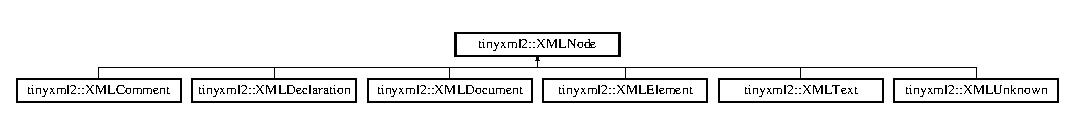
\includegraphics[height=1.145194cm]{classtinyxml2_1_1_x_m_l_node}
\end{center}
\end{figure}
\subsection*{Public Member Functions}
\begin{DoxyCompactItemize}
\item 
const \hyperlink{classtinyxml2_1_1_x_m_l_document}{X\-M\-L\-Document} $\ast$ \hyperlink{classtinyxml2_1_1_x_m_l_node_add244bca368083fa29698db8dcf147ca}{Get\-Document} () const 
\begin{DoxyCompactList}\small\item\em Get the \hyperlink{classtinyxml2_1_1_x_m_l_document}{X\-M\-L\-Document} that owns this \hyperlink{classtinyxml2_1_1_x_m_l_node}{X\-M\-L\-Node}. \end{DoxyCompactList}\item 
\hyperlink{classtinyxml2_1_1_x_m_l_document}{X\-M\-L\-Document} $\ast$ \hyperlink{classtinyxml2_1_1_x_m_l_node_af343d1ef0b45c0020e62d784d7e67a68}{Get\-Document} ()
\begin{DoxyCompactList}\small\item\em Get the \hyperlink{classtinyxml2_1_1_x_m_l_document}{X\-M\-L\-Document} that owns this \hyperlink{classtinyxml2_1_1_x_m_l_node}{X\-M\-L\-Node}. \end{DoxyCompactList}\item 
virtual \hyperlink{classtinyxml2_1_1_x_m_l_element}{X\-M\-L\-Element} $\ast$ \hyperlink{classtinyxml2_1_1_x_m_l_node_aab516e699567f75cc9ab2ef2eee501e8}{To\-Element} ()
\begin{DoxyCompactList}\small\item\em Safely cast to an Element, or null. \end{DoxyCompactList}\item 
virtual \hyperlink{classtinyxml2_1_1_x_m_l_text}{X\-M\-L\-Text} $\ast$ \hyperlink{classtinyxml2_1_1_x_m_l_node_a41c55dab9162d1eb62db2008430e376b}{To\-Text} ()
\begin{DoxyCompactList}\small\item\em Safely cast to Text, or null. \end{DoxyCompactList}\item 
virtual \hyperlink{classtinyxml2_1_1_x_m_l_comment}{X\-M\-L\-Comment} $\ast$ \hyperlink{classtinyxml2_1_1_x_m_l_node_aff47671055aa99840a1c1ebd661e63e3}{To\-Comment} ()
\begin{DoxyCompactList}\small\item\em Safely cast to a Comment, or null. \end{DoxyCompactList}\item 
virtual \hyperlink{classtinyxml2_1_1_x_m_l_document}{X\-M\-L\-Document} $\ast$ \hyperlink{classtinyxml2_1_1_x_m_l_node_a836e2966ed736fc3c94f70e12a2a3357}{To\-Document} ()
\begin{DoxyCompactList}\small\item\em Safely cast to a Document, or null. \end{DoxyCompactList}\item 
virtual \hyperlink{classtinyxml2_1_1_x_m_l_declaration}{X\-M\-L\-Declaration} $\ast$ \hyperlink{classtinyxml2_1_1_x_m_l_node_a174fd4c22c010b58138c1b84a0dfbd51}{To\-Declaration} ()
\begin{DoxyCompactList}\small\item\em Safely cast to a Declaration, or null. \end{DoxyCompactList}\item 
virtual \hyperlink{classtinyxml2_1_1_x_m_l_unknown}{X\-M\-L\-Unknown} $\ast$ \hyperlink{classtinyxml2_1_1_x_m_l_node_a8675a74aa0ada6eccab0c77ef3e5b9bd}{To\-Unknown} ()
\begin{DoxyCompactList}\small\item\em Safely cast to an Unknown, or null. \end{DoxyCompactList}\item 
virtual const \hyperlink{classtinyxml2_1_1_x_m_l_element}{X\-M\-L\-Element} $\ast$ \hyperlink{classtinyxml2_1_1_x_m_l_node_acbaec609797ddabb4f9dcf38ee91262e}{To\-Element} () const 
\item 
virtual const \hyperlink{classtinyxml2_1_1_x_m_l_text}{X\-M\-L\-Text} $\ast$ \hyperlink{classtinyxml2_1_1_x_m_l_node_a89009ffc1b9f5d692bf8d4c9f18c3bec}{To\-Text} () const 
\item 
virtual const \hyperlink{classtinyxml2_1_1_x_m_l_comment}{X\-M\-L\-Comment} $\ast$ \hyperlink{classtinyxml2_1_1_x_m_l_node_a157ce3a00ea5ee5a85b7103138e85e8a}{To\-Comment} () const 
\item 
virtual const \hyperlink{classtinyxml2_1_1_x_m_l_document}{X\-M\-L\-Document} $\ast$ \hyperlink{classtinyxml2_1_1_x_m_l_node_a3ff975733a17d6ced3539b45544c8bf6}{To\-Document} () const 
\item 
virtual const \hyperlink{classtinyxml2_1_1_x_m_l_declaration}{X\-M\-L\-Declaration} $\ast$ \hyperlink{classtinyxml2_1_1_x_m_l_node_aedae0bbb58d533a4b8a61042388b49e5}{To\-Declaration} () const 
\item 
virtual const \hyperlink{classtinyxml2_1_1_x_m_l_unknown}{X\-M\-L\-Unknown} $\ast$ \hyperlink{classtinyxml2_1_1_x_m_l_node_a71f5ae90296dbe67979f83fe97073efa}{To\-Unknown} () const 
\item 
const char $\ast$ \hyperlink{classtinyxml2_1_1_x_m_l_node_a92835c779871918f9af569bfe9669fe6}{Value} () const 
\item 
void \hyperlink{classtinyxml2_1_1_x_m_l_node_a09dd68cf9eae137579f6e50f36487513}{Set\-Value} (const char $\ast$val, bool static\-Mem=false)
\item 
const \hyperlink{classtinyxml2_1_1_x_m_l_node}{X\-M\-L\-Node} $\ast$ \hyperlink{classtinyxml2_1_1_x_m_l_node_a4e39bdcf9bfafa55d04857ece6aaf64e}{Parent} () const 
\begin{DoxyCompactList}\small\item\em Get the parent of this node on the D\-O\-M. \end{DoxyCompactList}\item 
\hyperlink{classtinyxml2_1_1_x_m_l_node}{X\-M\-L\-Node} $\ast$ \hyperlink{classtinyxml2_1_1_x_m_l_node_a76029693a5a54fbb721a41d7a0ca8a97}{Parent} ()
\item 
bool \hyperlink{classtinyxml2_1_1_x_m_l_node_a96afe34a9ccd0ed4c0cff32beb42cc6c}{No\-Children} () const 
\begin{DoxyCompactList}\small\item\em Returns true if this node has no children. \end{DoxyCompactList}\item 
const \hyperlink{classtinyxml2_1_1_x_m_l_node}{X\-M\-L\-Node} $\ast$ \hyperlink{classtinyxml2_1_1_x_m_l_node_a60e923d13d7dc01f45ab90a2f948b02a}{First\-Child} () const 
\begin{DoxyCompactList}\small\item\em Get the first child node, or null if none exists. \end{DoxyCompactList}\item 
\hyperlink{classtinyxml2_1_1_x_m_l_node}{X\-M\-L\-Node} $\ast$ \hyperlink{classtinyxml2_1_1_x_m_l_node_a2d6c70c475146b48bc93a7fafdeff5e0}{First\-Child} ()
\item 
const \hyperlink{classtinyxml2_1_1_x_m_l_element}{X\-M\-L\-Element} $\ast$ \hyperlink{classtinyxml2_1_1_x_m_l_node_a20f48e99b03e9c17487944f229bee130}{First\-Child\-Element} (const char $\ast$value=0) const 
\item 
\hyperlink{classtinyxml2_1_1_x_m_l_element}{X\-M\-L\-Element} $\ast$ \hyperlink{classtinyxml2_1_1_x_m_l_node_a7614c3b4eea1ff11b2aa90b0f92f6dba}{First\-Child\-Element} (const char $\ast$value=0)
\item 
const \hyperlink{classtinyxml2_1_1_x_m_l_node}{X\-M\-L\-Node} $\ast$ \hyperlink{classtinyxml2_1_1_x_m_l_node_a6088246532b02895beb0e6fa561a7f3b}{Last\-Child} () const 
\begin{DoxyCompactList}\small\item\em Get the last child node, or null if none exists. \end{DoxyCompactList}\item 
\hyperlink{classtinyxml2_1_1_x_m_l_node}{X\-M\-L\-Node} $\ast$ \hyperlink{classtinyxml2_1_1_x_m_l_node_ad7552c8cb1dc0cb6f3bdc14a9d115dbf}{Last\-Child} ()
\item 
const \hyperlink{classtinyxml2_1_1_x_m_l_element}{X\-M\-L\-Element} $\ast$ \hyperlink{classtinyxml2_1_1_x_m_l_node_a1a46cc01ece2216acf1e6294d1aff79d}{Last\-Child\-Element} (const char $\ast$value=0) const 
\item 
\hyperlink{classtinyxml2_1_1_x_m_l_element}{X\-M\-L\-Element} $\ast$ \hyperlink{classtinyxml2_1_1_x_m_l_node_a125423acf3170b130634638c5afc0639}{Last\-Child\-Element} (const char $\ast$value=0)
\item 
const \hyperlink{classtinyxml2_1_1_x_m_l_node}{X\-M\-L\-Node} $\ast$ \hyperlink{classtinyxml2_1_1_x_m_l_node_a4cb1bf63e9de55129d21a7be60685fd4}{Previous\-Sibling} () const 
\begin{DoxyCompactList}\small\item\em Get the previous (left) sibling node of this node. \end{DoxyCompactList}\item 
\hyperlink{classtinyxml2_1_1_x_m_l_node}{X\-M\-L\-Node} $\ast$ \hyperlink{classtinyxml2_1_1_x_m_l_node_ae760e5e7e766df1d2cf3bb4a847876d6}{Previous\-Sibling} ()
\item 
const \hyperlink{classtinyxml2_1_1_x_m_l_element}{X\-M\-L\-Element} $\ast$ \hyperlink{classtinyxml2_1_1_x_m_l_node_a573b2559c41dce244d893d610fbe0bd9}{Previous\-Sibling\-Element} (const char $\ast$value=0) const 
\begin{DoxyCompactList}\small\item\em Get the previous (left) sibling element of this node, with an optionally supplied name. \end{DoxyCompactList}\item 
\hyperlink{classtinyxml2_1_1_x_m_l_element}{X\-M\-L\-Element} $\ast$ \hyperlink{classtinyxml2_1_1_x_m_l_node_ae9177fdc49cb89879f333581d5f734f1}{Previous\-Sibling\-Element} (const char $\ast$value=0)
\item 
const \hyperlink{classtinyxml2_1_1_x_m_l_node}{X\-M\-L\-Node} $\ast$ \hyperlink{classtinyxml2_1_1_x_m_l_node_abba1df37581d89dccc45acdc55750ba2}{Next\-Sibling} () const 
\begin{DoxyCompactList}\small\item\em Get the next (right) sibling node of this node. \end{DoxyCompactList}\item 
\hyperlink{classtinyxml2_1_1_x_m_l_node}{X\-M\-L\-Node} $\ast$ \hyperlink{classtinyxml2_1_1_x_m_l_node_aeb7d4dfd8fb924ef86e7cb72183acbac}{Next\-Sibling} ()
\item 
const \hyperlink{classtinyxml2_1_1_x_m_l_element}{X\-M\-L\-Element} $\ast$ \hyperlink{classtinyxml2_1_1_x_m_l_node_a490e166c3a1c6607960bfa9c112d3d30}{Next\-Sibling\-Element} (const char $\ast$value=0) const 
\begin{DoxyCompactList}\small\item\em Get the next (right) sibling element of this node, with an optionally supplied name. \end{DoxyCompactList}\item 
\hyperlink{classtinyxml2_1_1_x_m_l_element}{X\-M\-L\-Element} $\ast$ \hyperlink{classtinyxml2_1_1_x_m_l_node_acf735bf653016792522305d8ad4b3029}{Next\-Sibling\-Element} (const char $\ast$value=0)
\item 
\hyperlink{classtinyxml2_1_1_x_m_l_node}{X\-M\-L\-Node} $\ast$ \hyperlink{classtinyxml2_1_1_x_m_l_node_ae3b422e98914d6002ca99bb1d2837103}{Insert\-End\-Child} (\hyperlink{classtinyxml2_1_1_x_m_l_node}{X\-M\-L\-Node} $\ast$add\-This)
\item 
\hyperlink{classtinyxml2_1_1_x_m_l_node}{X\-M\-L\-Node} $\ast$ \hyperlink{classtinyxml2_1_1_x_m_l_node_a663e3a5a378169fd477378f4d17a7649}{Link\-End\-Child} (\hyperlink{classtinyxml2_1_1_x_m_l_node}{X\-M\-L\-Node} $\ast$add\-This)
\item 
\hyperlink{classtinyxml2_1_1_x_m_l_node}{X\-M\-L\-Node} $\ast$ \hyperlink{classtinyxml2_1_1_x_m_l_node_ac609a8f3ea949027f439280c640bbaf2}{Insert\-First\-Child} (\hyperlink{classtinyxml2_1_1_x_m_l_node}{X\-M\-L\-Node} $\ast$add\-This)
\item 
\hyperlink{classtinyxml2_1_1_x_m_l_node}{X\-M\-L\-Node} $\ast$ \hyperlink{classtinyxml2_1_1_x_m_l_node_a9275138a1b8dd5d8e2c26789bdc23ac8}{Insert\-After\-Child} (\hyperlink{classtinyxml2_1_1_x_m_l_node}{X\-M\-L\-Node} $\ast$after\-This, \hyperlink{classtinyxml2_1_1_x_m_l_node}{X\-M\-L\-Node} $\ast$add\-This)
\item 
void \hyperlink{classtinyxml2_1_1_x_m_l_node_a0360085cc54df5bff85d5c5da13afdce}{Delete\-Children} ()
\item 
void \hyperlink{classtinyxml2_1_1_x_m_l_node_a363b6edbd6ebd55f8387d2b89f2b0921}{Delete\-Child} (\hyperlink{classtinyxml2_1_1_x_m_l_node}{X\-M\-L\-Node} $\ast$node)
\item 
virtual \hyperlink{classtinyxml2_1_1_x_m_l_node}{X\-M\-L\-Node} $\ast$ \hyperlink{classtinyxml2_1_1_x_m_l_node_a8402cbd3129d20e9e6024bbcc0531283}{Shallow\-Clone} (\hyperlink{classtinyxml2_1_1_x_m_l_document}{X\-M\-L\-Document} $\ast$document) const =0
\item 
virtual bool \hyperlink{classtinyxml2_1_1_x_m_l_node_a7ce18b751c3ea09eac292dca264f9226}{Shallow\-Equal} (const \hyperlink{classtinyxml2_1_1_x_m_l_node}{X\-M\-L\-Node} $\ast$compare) const =0
\item 
virtual bool \hyperlink{classtinyxml2_1_1_x_m_l_node_a81e66df0a44c67a7af17f3b77a152785}{Accept} (\hyperlink{classtinyxml2_1_1_x_m_l_visitor}{X\-M\-L\-Visitor} $\ast$visitor) const =0
\item 
virtual char $\ast$ \hyperlink{classtinyxml2_1_1_x_m_l_node_a7610d0f603e8b603d2078521811a23c1}{Parse\-Deep} (char $\ast$, \hyperlink{classtinyxml2_1_1_str_pair}{Str\-Pair} $\ast$)
\end{DoxyCompactItemize}
\subsection*{Protected Member Functions}
\begin{DoxyCompactItemize}
\item 
\hyperlink{classtinyxml2_1_1_x_m_l_node_a29868df6ca383d574f584dfdd15105b6}{X\-M\-L\-Node} (\hyperlink{classtinyxml2_1_1_x_m_l_document}{X\-M\-L\-Document} $\ast$)
\item 
virtual \hyperlink{classtinyxml2_1_1_x_m_l_node_a8f41e898cdd4da4cdbb7f05b0c7d9f69}{$\sim$\-X\-M\-L\-Node} ()
\item 
\hyperlink{classtinyxml2_1_1_x_m_l_node_a78be01384518a969da905548f318d75b}{X\-M\-L\-Node} (const \hyperlink{classtinyxml2_1_1_x_m_l_node}{X\-M\-L\-Node} \&)
\item 
\hyperlink{classtinyxml2_1_1_x_m_l_node}{X\-M\-L\-Node} \& \hyperlink{classtinyxml2_1_1_x_m_l_node_ade79231d908e1f21862819e00e56ab6e}{operator=} (const \hyperlink{classtinyxml2_1_1_x_m_l_node}{X\-M\-L\-Node} \&)
\end{DoxyCompactItemize}
\subsection*{Protected Attributes}
\begin{DoxyCompactItemize}
\item 
\hyperlink{classtinyxml2_1_1_x_m_l_document}{X\-M\-L\-Document} $\ast$ \hyperlink{classtinyxml2_1_1_x_m_l_node_a8d2d2be0bb6797625551eb0e91f0ff62}{\-\_\-document}
\item 
\hyperlink{classtinyxml2_1_1_x_m_l_node}{X\-M\-L\-Node} $\ast$ \hyperlink{classtinyxml2_1_1_x_m_l_node_a176dd1c4965c21c366de192164aa2c13}{\-\_\-parent}
\item 
\hyperlink{classtinyxml2_1_1_str_pair}{Str\-Pair} \hyperlink{classtinyxml2_1_1_x_m_l_node_a3ea9884098b8379de2bb5ab3fc85c0fc}{\-\_\-value}
\item 
\hyperlink{classtinyxml2_1_1_x_m_l_node}{X\-M\-L\-Node} $\ast$ \hyperlink{classtinyxml2_1_1_x_m_l_node_aa20c91e4213dc930c5bdf420322ca342}{\-\_\-first\-Child}
\item 
\hyperlink{classtinyxml2_1_1_x_m_l_node}{X\-M\-L\-Node} $\ast$ \hyperlink{classtinyxml2_1_1_x_m_l_node_a099b6560ae44ab9edb8453aaf1a3747b}{\-\_\-last\-Child}
\item 
\hyperlink{classtinyxml2_1_1_x_m_l_node}{X\-M\-L\-Node} $\ast$ \hyperlink{classtinyxml2_1_1_x_m_l_node_a9739eb0fb9a1188266052055e7a6bf6b}{\-\_\-prev}
\item 
\hyperlink{classtinyxml2_1_1_x_m_l_node}{X\-M\-L\-Node} $\ast$ \hyperlink{classtinyxml2_1_1_x_m_l_node_a27e985496b37dd00eb5b9cf59b9e3fb1}{\-\_\-next}
\end{DoxyCompactItemize}
\subsection*{Private Member Functions}
\begin{DoxyCompactItemize}
\item 
void \hyperlink{classtinyxml2_1_1_x_m_l_node_a9546e242b6a4f232415befb1cfe0fdd4}{Unlink} (\hyperlink{classtinyxml2_1_1_x_m_l_node}{X\-M\-L\-Node} $\ast$child)
\end{DoxyCompactItemize}
\subsection*{Private Attributes}
\begin{DoxyCompactItemize}
\item 
\hyperlink{classtinyxml2_1_1_mem_pool}{Mem\-Pool} $\ast$ \hyperlink{classtinyxml2_1_1_x_m_l_node_a4e3ff179bc312480b6bc3e57014834f7}{\-\_\-mem\-Pool}
\end{DoxyCompactItemize}
\subsection*{Friends}
\begin{DoxyCompactItemize}
\item 
class \hyperlink{classtinyxml2_1_1_x_m_l_node_a4eee3bda60c60a30e4e8cd4ea91c4c6e}{X\-M\-L\-Document}
\item 
class \hyperlink{classtinyxml2_1_1_x_m_l_node_ac2fba9b6e452829dd892f7392c24e0eb}{X\-M\-L\-Element}
\end{DoxyCompactItemize}


\subsection{Detailed Description}
\hyperlink{classtinyxml2_1_1_x_m_l_node}{X\-M\-L\-Node} is a base class for every object that is in the X\-M\-L Document Object Model (D\-O\-M), except X\-M\-L\-Attributes. Nodes have siblings, a parent, and children which can be navigated. A node is always in a \hyperlink{classtinyxml2_1_1_x_m_l_document}{X\-M\-L\-Document}. The type of a \hyperlink{classtinyxml2_1_1_x_m_l_node}{X\-M\-L\-Node} can be queried, and it can be cast to its more defined type.

A \hyperlink{classtinyxml2_1_1_x_m_l_document}{X\-M\-L\-Document} allocates memory for all its Nodes. When the \hyperlink{classtinyxml2_1_1_x_m_l_document}{X\-M\-L\-Document} gets deleted, all its Nodes will also be deleted.

\begin{DoxyVerb}A Document can contain: Element (container or leaf)
                        Comment (leaf)
                        Unknown (leaf)
                        Declaration( leaf )

An Element can contain: Element (container or leaf)
                        Text    (leaf)
                        Attributes (not on tree)
                        Comment (leaf)
                        Unknown (leaf)\end{DoxyVerb}
 

\subsection{Constructor \& Destructor Documentation}
\hypertarget{classtinyxml2_1_1_x_m_l_node_a29868df6ca383d574f584dfdd15105b6}{\index{tinyxml2\-::\-X\-M\-L\-Node@{tinyxml2\-::\-X\-M\-L\-Node}!X\-M\-L\-Node@{X\-M\-L\-Node}}
\index{X\-M\-L\-Node@{X\-M\-L\-Node}!tinyxml2::XMLNode@{tinyxml2\-::\-X\-M\-L\-Node}}
\subsubsection[{X\-M\-L\-Node}]{\setlength{\rightskip}{0pt plus 5cm}tinyxml2\-::\-X\-M\-L\-Node\-::\-X\-M\-L\-Node (
\begin{DoxyParamCaption}
\item[{{\bf X\-M\-L\-Document} $\ast$}]{doc}
\end{DoxyParamCaption}
)\hspace{0.3cm}{\ttfamily [protected]}}}\label{classtinyxml2_1_1_x_m_l_node_a29868df6ca383d574f584dfdd15105b6}
\hypertarget{classtinyxml2_1_1_x_m_l_node_a8f41e898cdd4da4cdbb7f05b0c7d9f69}{\index{tinyxml2\-::\-X\-M\-L\-Node@{tinyxml2\-::\-X\-M\-L\-Node}!$\sim$\-X\-M\-L\-Node@{$\sim$\-X\-M\-L\-Node}}
\index{$\sim$\-X\-M\-L\-Node@{$\sim$\-X\-M\-L\-Node}!tinyxml2::XMLNode@{tinyxml2\-::\-X\-M\-L\-Node}}
\subsubsection[{$\sim$\-X\-M\-L\-Node}]{\setlength{\rightskip}{0pt plus 5cm}tinyxml2\-::\-X\-M\-L\-Node\-::$\sim$\-X\-M\-L\-Node (
\begin{DoxyParamCaption}
{}
\end{DoxyParamCaption}
)\hspace{0.3cm}{\ttfamily [protected]}, {\ttfamily [virtual]}}}\label{classtinyxml2_1_1_x_m_l_node_a8f41e898cdd4da4cdbb7f05b0c7d9f69}
\hypertarget{classtinyxml2_1_1_x_m_l_node_a78be01384518a969da905548f318d75b}{\index{tinyxml2\-::\-X\-M\-L\-Node@{tinyxml2\-::\-X\-M\-L\-Node}!X\-M\-L\-Node@{X\-M\-L\-Node}}
\index{X\-M\-L\-Node@{X\-M\-L\-Node}!tinyxml2::XMLNode@{tinyxml2\-::\-X\-M\-L\-Node}}
\subsubsection[{X\-M\-L\-Node}]{\setlength{\rightskip}{0pt plus 5cm}tinyxml2\-::\-X\-M\-L\-Node\-::\-X\-M\-L\-Node (
\begin{DoxyParamCaption}
\item[{const {\bf X\-M\-L\-Node} \&}]{}
\end{DoxyParamCaption}
)\hspace{0.3cm}{\ttfamily [protected]}}}\label{classtinyxml2_1_1_x_m_l_node_a78be01384518a969da905548f318d75b}


\subsection{Member Function Documentation}
\hypertarget{classtinyxml2_1_1_x_m_l_node_a81e66df0a44c67a7af17f3b77a152785}{\index{tinyxml2\-::\-X\-M\-L\-Node@{tinyxml2\-::\-X\-M\-L\-Node}!Accept@{Accept}}
\index{Accept@{Accept}!tinyxml2::XMLNode@{tinyxml2\-::\-X\-M\-L\-Node}}
\subsubsection[{Accept}]{\setlength{\rightskip}{0pt plus 5cm}virtual bool tinyxml2\-::\-X\-M\-L\-Node\-::\-Accept (
\begin{DoxyParamCaption}
\item[{{\bf X\-M\-L\-Visitor} $\ast$}]{visitor}
\end{DoxyParamCaption}
) const\hspace{0.3cm}{\ttfamily [pure virtual]}}}\label{classtinyxml2_1_1_x_m_l_node_a81e66df0a44c67a7af17f3b77a152785}
Accept a hierarchical visit of the nodes in the Tiny\-X\-M\-L-\/2 D\-O\-M. Every node in the X\-M\-L tree will be conditionally visited and the host will be called back via the \hyperlink{classtinyxml2_1_1_x_m_l_visitor}{X\-M\-L\-Visitor} interface.

This is essentially a S\-A\-X interface for Tiny\-X\-M\-L-\/2. (Note however it doesn't re-\/parse the X\-M\-L for the callbacks, so the performance of Tiny\-X\-M\-L-\/2 is unchanged by using this interface versus any other.)

The interface has been based on ideas from\-:
\begin{DoxyItemize}
\item \href{http://www.saxproject.org/}{\tt http\-://www.\-saxproject.\-org/}
\item \href{http://c2.com/cgi/wiki?HierarchicalVisitorPattern}{\tt http\-://c2.\-com/cgi/wiki?\-Hierarchical\-Visitor\-Pattern}
\end{DoxyItemize}

Which are both good references for \char`\"{}visiting\char`\"{}.

An example of using \hyperlink{classtinyxml2_1_1_x_m_l_node_a81e66df0a44c67a7af17f3b77a152785}{Accept()}\-: \begin{DoxyVerb}XMLPrinter printer;
tinyxmlDoc.Accept( &printer );
const char* xmlcstr = printer.CStr();
\end{DoxyVerb}
 

Implemented in \hyperlink{classtinyxml2_1_1_x_m_l_document_aa08503d24898bf9992ae5e5fb8b0cf87}{tinyxml2\-::\-X\-M\-L\-Document}, \hyperlink{classtinyxml2_1_1_x_m_l_element_a36d65438991a1e85096caf39ad13a099}{tinyxml2\-::\-X\-M\-L\-Element}, \hyperlink{classtinyxml2_1_1_x_m_l_unknown_a0d341ab804a1438a474810bb5bd29dd5}{tinyxml2\-::\-X\-M\-L\-Unknown}, \hyperlink{classtinyxml2_1_1_x_m_l_declaration_a953a7359cc312d15218eb5843a4ca108}{tinyxml2\-::\-X\-M\-L\-Declaration}, \hyperlink{classtinyxml2_1_1_x_m_l_comment_aa382b1be6a8b0650c16a2d88bb499335}{tinyxml2\-::\-X\-M\-L\-Comment}, and \hyperlink{classtinyxml2_1_1_x_m_l_text_ae659d4fc7351a7df11c111cbe1ade46f}{tinyxml2\-::\-X\-M\-L\-Text}.

\hypertarget{classtinyxml2_1_1_x_m_l_node_a363b6edbd6ebd55f8387d2b89f2b0921}{\index{tinyxml2\-::\-X\-M\-L\-Node@{tinyxml2\-::\-X\-M\-L\-Node}!Delete\-Child@{Delete\-Child}}
\index{Delete\-Child@{Delete\-Child}!tinyxml2::XMLNode@{tinyxml2\-::\-X\-M\-L\-Node}}
\subsubsection[{Delete\-Child}]{\setlength{\rightskip}{0pt plus 5cm}void tinyxml2\-::\-X\-M\-L\-Node\-::\-Delete\-Child (
\begin{DoxyParamCaption}
\item[{{\bf X\-M\-L\-Node} $\ast$}]{node}
\end{DoxyParamCaption}
)}}\label{classtinyxml2_1_1_x_m_l_node_a363b6edbd6ebd55f8387d2b89f2b0921}
Delete a child of this node. \hypertarget{classtinyxml2_1_1_x_m_l_node_a0360085cc54df5bff85d5c5da13afdce}{\index{tinyxml2\-::\-X\-M\-L\-Node@{tinyxml2\-::\-X\-M\-L\-Node}!Delete\-Children@{Delete\-Children}}
\index{Delete\-Children@{Delete\-Children}!tinyxml2::XMLNode@{tinyxml2\-::\-X\-M\-L\-Node}}
\subsubsection[{Delete\-Children}]{\setlength{\rightskip}{0pt plus 5cm}void tinyxml2\-::\-X\-M\-L\-Node\-::\-Delete\-Children (
\begin{DoxyParamCaption}
{}
\end{DoxyParamCaption}
)}}\label{classtinyxml2_1_1_x_m_l_node_a0360085cc54df5bff85d5c5da13afdce}
Delete all the children of this node. \hypertarget{classtinyxml2_1_1_x_m_l_node_a60e923d13d7dc01f45ab90a2f948b02a}{\index{tinyxml2\-::\-X\-M\-L\-Node@{tinyxml2\-::\-X\-M\-L\-Node}!First\-Child@{First\-Child}}
\index{First\-Child@{First\-Child}!tinyxml2::XMLNode@{tinyxml2\-::\-X\-M\-L\-Node}}
\subsubsection[{First\-Child}]{\setlength{\rightskip}{0pt plus 5cm}const {\bf X\-M\-L\-Node}$\ast$ tinyxml2\-::\-X\-M\-L\-Node\-::\-First\-Child (
\begin{DoxyParamCaption}
{}
\end{DoxyParamCaption}
) const\hspace{0.3cm}{\ttfamily [inline]}}}\label{classtinyxml2_1_1_x_m_l_node_a60e923d13d7dc01f45ab90a2f948b02a}


Get the first child node, or null if none exists. 

\hypertarget{classtinyxml2_1_1_x_m_l_node_a2d6c70c475146b48bc93a7fafdeff5e0}{\index{tinyxml2\-::\-X\-M\-L\-Node@{tinyxml2\-::\-X\-M\-L\-Node}!First\-Child@{First\-Child}}
\index{First\-Child@{First\-Child}!tinyxml2::XMLNode@{tinyxml2\-::\-X\-M\-L\-Node}}
\subsubsection[{First\-Child}]{\setlength{\rightskip}{0pt plus 5cm}{\bf X\-M\-L\-Node}$\ast$ tinyxml2\-::\-X\-M\-L\-Node\-::\-First\-Child (
\begin{DoxyParamCaption}
{}
\end{DoxyParamCaption}
)\hspace{0.3cm}{\ttfamily [inline]}}}\label{classtinyxml2_1_1_x_m_l_node_a2d6c70c475146b48bc93a7fafdeff5e0}
\hypertarget{classtinyxml2_1_1_x_m_l_node_a20f48e99b03e9c17487944f229bee130}{\index{tinyxml2\-::\-X\-M\-L\-Node@{tinyxml2\-::\-X\-M\-L\-Node}!First\-Child\-Element@{First\-Child\-Element}}
\index{First\-Child\-Element@{First\-Child\-Element}!tinyxml2::XMLNode@{tinyxml2\-::\-X\-M\-L\-Node}}
\subsubsection[{First\-Child\-Element}]{\setlength{\rightskip}{0pt plus 5cm}const {\bf X\-M\-L\-Element} $\ast$ tinyxml2\-::\-X\-M\-L\-Node\-::\-First\-Child\-Element (
\begin{DoxyParamCaption}
\item[{const char $\ast$}]{value = {\ttfamily 0}}
\end{DoxyParamCaption}
) const}}\label{classtinyxml2_1_1_x_m_l_node_a20f48e99b03e9c17487944f229bee130}
Get the first child element, or optionally the first child element with the specified name. \hypertarget{classtinyxml2_1_1_x_m_l_node_a7614c3b4eea1ff11b2aa90b0f92f6dba}{\index{tinyxml2\-::\-X\-M\-L\-Node@{tinyxml2\-::\-X\-M\-L\-Node}!First\-Child\-Element@{First\-Child\-Element}}
\index{First\-Child\-Element@{First\-Child\-Element}!tinyxml2::XMLNode@{tinyxml2\-::\-X\-M\-L\-Node}}
\subsubsection[{First\-Child\-Element}]{\setlength{\rightskip}{0pt plus 5cm}{\bf X\-M\-L\-Element}$\ast$ tinyxml2\-::\-X\-M\-L\-Node\-::\-First\-Child\-Element (
\begin{DoxyParamCaption}
\item[{const char $\ast$}]{value = {\ttfamily 0}}
\end{DoxyParamCaption}
)\hspace{0.3cm}{\ttfamily [inline]}}}\label{classtinyxml2_1_1_x_m_l_node_a7614c3b4eea1ff11b2aa90b0f92f6dba}
\hypertarget{classtinyxml2_1_1_x_m_l_node_add244bca368083fa29698db8dcf147ca}{\index{tinyxml2\-::\-X\-M\-L\-Node@{tinyxml2\-::\-X\-M\-L\-Node}!Get\-Document@{Get\-Document}}
\index{Get\-Document@{Get\-Document}!tinyxml2::XMLNode@{tinyxml2\-::\-X\-M\-L\-Node}}
\subsubsection[{Get\-Document}]{\setlength{\rightskip}{0pt plus 5cm}const {\bf X\-M\-L\-Document}$\ast$ tinyxml2\-::\-X\-M\-L\-Node\-::\-Get\-Document (
\begin{DoxyParamCaption}
{}
\end{DoxyParamCaption}
) const\hspace{0.3cm}{\ttfamily [inline]}}}\label{classtinyxml2_1_1_x_m_l_node_add244bca368083fa29698db8dcf147ca}


Get the \hyperlink{classtinyxml2_1_1_x_m_l_document}{X\-M\-L\-Document} that owns this \hyperlink{classtinyxml2_1_1_x_m_l_node}{X\-M\-L\-Node}. 

\hypertarget{classtinyxml2_1_1_x_m_l_node_af343d1ef0b45c0020e62d784d7e67a68}{\index{tinyxml2\-::\-X\-M\-L\-Node@{tinyxml2\-::\-X\-M\-L\-Node}!Get\-Document@{Get\-Document}}
\index{Get\-Document@{Get\-Document}!tinyxml2::XMLNode@{tinyxml2\-::\-X\-M\-L\-Node}}
\subsubsection[{Get\-Document}]{\setlength{\rightskip}{0pt plus 5cm}{\bf X\-M\-L\-Document}$\ast$ tinyxml2\-::\-X\-M\-L\-Node\-::\-Get\-Document (
\begin{DoxyParamCaption}
{}
\end{DoxyParamCaption}
)\hspace{0.3cm}{\ttfamily [inline]}}}\label{classtinyxml2_1_1_x_m_l_node_af343d1ef0b45c0020e62d784d7e67a68}


Get the \hyperlink{classtinyxml2_1_1_x_m_l_document}{X\-M\-L\-Document} that owns this \hyperlink{classtinyxml2_1_1_x_m_l_node}{X\-M\-L\-Node}. 

\hypertarget{classtinyxml2_1_1_x_m_l_node_a9275138a1b8dd5d8e2c26789bdc23ac8}{\index{tinyxml2\-::\-X\-M\-L\-Node@{tinyxml2\-::\-X\-M\-L\-Node}!Insert\-After\-Child@{Insert\-After\-Child}}
\index{Insert\-After\-Child@{Insert\-After\-Child}!tinyxml2::XMLNode@{tinyxml2\-::\-X\-M\-L\-Node}}
\subsubsection[{Insert\-After\-Child}]{\setlength{\rightskip}{0pt plus 5cm}{\bf X\-M\-L\-Node} $\ast$ tinyxml2\-::\-X\-M\-L\-Node\-::\-Insert\-After\-Child (
\begin{DoxyParamCaption}
\item[{{\bf X\-M\-L\-Node} $\ast$}]{after\-This, }
\item[{{\bf X\-M\-L\-Node} $\ast$}]{add\-This}
\end{DoxyParamCaption}
)}}\label{classtinyxml2_1_1_x_m_l_node_a9275138a1b8dd5d8e2c26789bdc23ac8}
Add a node after the specified child node. If the child node is already part of the document, it is moved from its old location to the new location. Returns the add\-This argument or 0 if the after\-This node is not a child of this node, or if the node does not belong to the same document. \hypertarget{classtinyxml2_1_1_x_m_l_node_ae3b422e98914d6002ca99bb1d2837103}{\index{tinyxml2\-::\-X\-M\-L\-Node@{tinyxml2\-::\-X\-M\-L\-Node}!Insert\-End\-Child@{Insert\-End\-Child}}
\index{Insert\-End\-Child@{Insert\-End\-Child}!tinyxml2::XMLNode@{tinyxml2\-::\-X\-M\-L\-Node}}
\subsubsection[{Insert\-End\-Child}]{\setlength{\rightskip}{0pt plus 5cm}{\bf X\-M\-L\-Node} $\ast$ tinyxml2\-::\-X\-M\-L\-Node\-::\-Insert\-End\-Child (
\begin{DoxyParamCaption}
\item[{{\bf X\-M\-L\-Node} $\ast$}]{add\-This}
\end{DoxyParamCaption}
)}}\label{classtinyxml2_1_1_x_m_l_node_ae3b422e98914d6002ca99bb1d2837103}
Add a child node as the last (right) child. If the child node is already part of the document, it is moved from its old location to the new location. Returns the add\-This argument or 0 if the node does not belong to the same document. \hypertarget{classtinyxml2_1_1_x_m_l_node_ac609a8f3ea949027f439280c640bbaf2}{\index{tinyxml2\-::\-X\-M\-L\-Node@{tinyxml2\-::\-X\-M\-L\-Node}!Insert\-First\-Child@{Insert\-First\-Child}}
\index{Insert\-First\-Child@{Insert\-First\-Child}!tinyxml2::XMLNode@{tinyxml2\-::\-X\-M\-L\-Node}}
\subsubsection[{Insert\-First\-Child}]{\setlength{\rightskip}{0pt plus 5cm}{\bf X\-M\-L\-Node} $\ast$ tinyxml2\-::\-X\-M\-L\-Node\-::\-Insert\-First\-Child (
\begin{DoxyParamCaption}
\item[{{\bf X\-M\-L\-Node} $\ast$}]{add\-This}
\end{DoxyParamCaption}
)}}\label{classtinyxml2_1_1_x_m_l_node_ac609a8f3ea949027f439280c640bbaf2}
Add a child node as the first (left) child. If the child node is already part of the document, it is moved from its old location to the new location. Returns the add\-This argument or 0 if the node does not belong to the same document. \hypertarget{classtinyxml2_1_1_x_m_l_node_a6088246532b02895beb0e6fa561a7f3b}{\index{tinyxml2\-::\-X\-M\-L\-Node@{tinyxml2\-::\-X\-M\-L\-Node}!Last\-Child@{Last\-Child}}
\index{Last\-Child@{Last\-Child}!tinyxml2::XMLNode@{tinyxml2\-::\-X\-M\-L\-Node}}
\subsubsection[{Last\-Child}]{\setlength{\rightskip}{0pt plus 5cm}const {\bf X\-M\-L\-Node}$\ast$ tinyxml2\-::\-X\-M\-L\-Node\-::\-Last\-Child (
\begin{DoxyParamCaption}
{}
\end{DoxyParamCaption}
) const\hspace{0.3cm}{\ttfamily [inline]}}}\label{classtinyxml2_1_1_x_m_l_node_a6088246532b02895beb0e6fa561a7f3b}


Get the last child node, or null if none exists. 

\hypertarget{classtinyxml2_1_1_x_m_l_node_ad7552c8cb1dc0cb6f3bdc14a9d115dbf}{\index{tinyxml2\-::\-X\-M\-L\-Node@{tinyxml2\-::\-X\-M\-L\-Node}!Last\-Child@{Last\-Child}}
\index{Last\-Child@{Last\-Child}!tinyxml2::XMLNode@{tinyxml2\-::\-X\-M\-L\-Node}}
\subsubsection[{Last\-Child}]{\setlength{\rightskip}{0pt plus 5cm}{\bf X\-M\-L\-Node}$\ast$ tinyxml2\-::\-X\-M\-L\-Node\-::\-Last\-Child (
\begin{DoxyParamCaption}
{}
\end{DoxyParamCaption}
)\hspace{0.3cm}{\ttfamily [inline]}}}\label{classtinyxml2_1_1_x_m_l_node_ad7552c8cb1dc0cb6f3bdc14a9d115dbf}
\hypertarget{classtinyxml2_1_1_x_m_l_node_a1a46cc01ece2216acf1e6294d1aff79d}{\index{tinyxml2\-::\-X\-M\-L\-Node@{tinyxml2\-::\-X\-M\-L\-Node}!Last\-Child\-Element@{Last\-Child\-Element}}
\index{Last\-Child\-Element@{Last\-Child\-Element}!tinyxml2::XMLNode@{tinyxml2\-::\-X\-M\-L\-Node}}
\subsubsection[{Last\-Child\-Element}]{\setlength{\rightskip}{0pt plus 5cm}const {\bf X\-M\-L\-Element} $\ast$ tinyxml2\-::\-X\-M\-L\-Node\-::\-Last\-Child\-Element (
\begin{DoxyParamCaption}
\item[{const char $\ast$}]{value = {\ttfamily 0}}
\end{DoxyParamCaption}
) const}}\label{classtinyxml2_1_1_x_m_l_node_a1a46cc01ece2216acf1e6294d1aff79d}
Get the last child element or optionally the last child element with the specified name. \hypertarget{classtinyxml2_1_1_x_m_l_node_a125423acf3170b130634638c5afc0639}{\index{tinyxml2\-::\-X\-M\-L\-Node@{tinyxml2\-::\-X\-M\-L\-Node}!Last\-Child\-Element@{Last\-Child\-Element}}
\index{Last\-Child\-Element@{Last\-Child\-Element}!tinyxml2::XMLNode@{tinyxml2\-::\-X\-M\-L\-Node}}
\subsubsection[{Last\-Child\-Element}]{\setlength{\rightskip}{0pt plus 5cm}{\bf X\-M\-L\-Element}$\ast$ tinyxml2\-::\-X\-M\-L\-Node\-::\-Last\-Child\-Element (
\begin{DoxyParamCaption}
\item[{const char $\ast$}]{value = {\ttfamily 0}}
\end{DoxyParamCaption}
)\hspace{0.3cm}{\ttfamily [inline]}}}\label{classtinyxml2_1_1_x_m_l_node_a125423acf3170b130634638c5afc0639}
\hypertarget{classtinyxml2_1_1_x_m_l_node_a663e3a5a378169fd477378f4d17a7649}{\index{tinyxml2\-::\-X\-M\-L\-Node@{tinyxml2\-::\-X\-M\-L\-Node}!Link\-End\-Child@{Link\-End\-Child}}
\index{Link\-End\-Child@{Link\-End\-Child}!tinyxml2::XMLNode@{tinyxml2\-::\-X\-M\-L\-Node}}
\subsubsection[{Link\-End\-Child}]{\setlength{\rightskip}{0pt plus 5cm}{\bf X\-M\-L\-Node}$\ast$ tinyxml2\-::\-X\-M\-L\-Node\-::\-Link\-End\-Child (
\begin{DoxyParamCaption}
\item[{{\bf X\-M\-L\-Node} $\ast$}]{add\-This}
\end{DoxyParamCaption}
)\hspace{0.3cm}{\ttfamily [inline]}}}\label{classtinyxml2_1_1_x_m_l_node_a663e3a5a378169fd477378f4d17a7649}
\hypertarget{classtinyxml2_1_1_x_m_l_node_abba1df37581d89dccc45acdc55750ba2}{\index{tinyxml2\-::\-X\-M\-L\-Node@{tinyxml2\-::\-X\-M\-L\-Node}!Next\-Sibling@{Next\-Sibling}}
\index{Next\-Sibling@{Next\-Sibling}!tinyxml2::XMLNode@{tinyxml2\-::\-X\-M\-L\-Node}}
\subsubsection[{Next\-Sibling}]{\setlength{\rightskip}{0pt plus 5cm}const {\bf X\-M\-L\-Node}$\ast$ tinyxml2\-::\-X\-M\-L\-Node\-::\-Next\-Sibling (
\begin{DoxyParamCaption}
{}
\end{DoxyParamCaption}
) const\hspace{0.3cm}{\ttfamily [inline]}}}\label{classtinyxml2_1_1_x_m_l_node_abba1df37581d89dccc45acdc55750ba2}


Get the next (right) sibling node of this node. 

\hypertarget{classtinyxml2_1_1_x_m_l_node_aeb7d4dfd8fb924ef86e7cb72183acbac}{\index{tinyxml2\-::\-X\-M\-L\-Node@{tinyxml2\-::\-X\-M\-L\-Node}!Next\-Sibling@{Next\-Sibling}}
\index{Next\-Sibling@{Next\-Sibling}!tinyxml2::XMLNode@{tinyxml2\-::\-X\-M\-L\-Node}}
\subsubsection[{Next\-Sibling}]{\setlength{\rightskip}{0pt plus 5cm}{\bf X\-M\-L\-Node}$\ast$ tinyxml2\-::\-X\-M\-L\-Node\-::\-Next\-Sibling (
\begin{DoxyParamCaption}
{}
\end{DoxyParamCaption}
)\hspace{0.3cm}{\ttfamily [inline]}}}\label{classtinyxml2_1_1_x_m_l_node_aeb7d4dfd8fb924ef86e7cb72183acbac}
\hypertarget{classtinyxml2_1_1_x_m_l_node_a490e166c3a1c6607960bfa9c112d3d30}{\index{tinyxml2\-::\-X\-M\-L\-Node@{tinyxml2\-::\-X\-M\-L\-Node}!Next\-Sibling\-Element@{Next\-Sibling\-Element}}
\index{Next\-Sibling\-Element@{Next\-Sibling\-Element}!tinyxml2::XMLNode@{tinyxml2\-::\-X\-M\-L\-Node}}
\subsubsection[{Next\-Sibling\-Element}]{\setlength{\rightskip}{0pt plus 5cm}const {\bf X\-M\-L\-Element} $\ast$ tinyxml2\-::\-X\-M\-L\-Node\-::\-Next\-Sibling\-Element (
\begin{DoxyParamCaption}
\item[{const char $\ast$}]{value = {\ttfamily 0}}
\end{DoxyParamCaption}
) const}}\label{classtinyxml2_1_1_x_m_l_node_a490e166c3a1c6607960bfa9c112d3d30}


Get the next (right) sibling element of this node, with an optionally supplied name. 

\hypertarget{classtinyxml2_1_1_x_m_l_node_acf735bf653016792522305d8ad4b3029}{\index{tinyxml2\-::\-X\-M\-L\-Node@{tinyxml2\-::\-X\-M\-L\-Node}!Next\-Sibling\-Element@{Next\-Sibling\-Element}}
\index{Next\-Sibling\-Element@{Next\-Sibling\-Element}!tinyxml2::XMLNode@{tinyxml2\-::\-X\-M\-L\-Node}}
\subsubsection[{Next\-Sibling\-Element}]{\setlength{\rightskip}{0pt plus 5cm}{\bf X\-M\-L\-Element}$\ast$ tinyxml2\-::\-X\-M\-L\-Node\-::\-Next\-Sibling\-Element (
\begin{DoxyParamCaption}
\item[{const char $\ast$}]{value = {\ttfamily 0}}
\end{DoxyParamCaption}
)\hspace{0.3cm}{\ttfamily [inline]}}}\label{classtinyxml2_1_1_x_m_l_node_acf735bf653016792522305d8ad4b3029}
\hypertarget{classtinyxml2_1_1_x_m_l_node_a96afe34a9ccd0ed4c0cff32beb42cc6c}{\index{tinyxml2\-::\-X\-M\-L\-Node@{tinyxml2\-::\-X\-M\-L\-Node}!No\-Children@{No\-Children}}
\index{No\-Children@{No\-Children}!tinyxml2::XMLNode@{tinyxml2\-::\-X\-M\-L\-Node}}
\subsubsection[{No\-Children}]{\setlength{\rightskip}{0pt plus 5cm}bool tinyxml2\-::\-X\-M\-L\-Node\-::\-No\-Children (
\begin{DoxyParamCaption}
{}
\end{DoxyParamCaption}
) const\hspace{0.3cm}{\ttfamily [inline]}}}\label{classtinyxml2_1_1_x_m_l_node_a96afe34a9ccd0ed4c0cff32beb42cc6c}


Returns true if this node has no children. 

\hypertarget{classtinyxml2_1_1_x_m_l_node_ade79231d908e1f21862819e00e56ab6e}{\index{tinyxml2\-::\-X\-M\-L\-Node@{tinyxml2\-::\-X\-M\-L\-Node}!operator=@{operator=}}
\index{operator=@{operator=}!tinyxml2::XMLNode@{tinyxml2\-::\-X\-M\-L\-Node}}
\subsubsection[{operator=}]{\setlength{\rightskip}{0pt plus 5cm}{\bf X\-M\-L\-Node}\& tinyxml2\-::\-X\-M\-L\-Node\-::operator= (
\begin{DoxyParamCaption}
\item[{const {\bf X\-M\-L\-Node} \&}]{}
\end{DoxyParamCaption}
)\hspace{0.3cm}{\ttfamily [protected]}}}\label{classtinyxml2_1_1_x_m_l_node_ade79231d908e1f21862819e00e56ab6e}
\hypertarget{classtinyxml2_1_1_x_m_l_node_a4e39bdcf9bfafa55d04857ece6aaf64e}{\index{tinyxml2\-::\-X\-M\-L\-Node@{tinyxml2\-::\-X\-M\-L\-Node}!Parent@{Parent}}
\index{Parent@{Parent}!tinyxml2::XMLNode@{tinyxml2\-::\-X\-M\-L\-Node}}
\subsubsection[{Parent}]{\setlength{\rightskip}{0pt plus 5cm}const {\bf X\-M\-L\-Node}$\ast$ tinyxml2\-::\-X\-M\-L\-Node\-::\-Parent (
\begin{DoxyParamCaption}
{}
\end{DoxyParamCaption}
) const\hspace{0.3cm}{\ttfamily [inline]}}}\label{classtinyxml2_1_1_x_m_l_node_a4e39bdcf9bfafa55d04857ece6aaf64e}


Get the parent of this node on the D\-O\-M. 

\hypertarget{classtinyxml2_1_1_x_m_l_node_a76029693a5a54fbb721a41d7a0ca8a97}{\index{tinyxml2\-::\-X\-M\-L\-Node@{tinyxml2\-::\-X\-M\-L\-Node}!Parent@{Parent}}
\index{Parent@{Parent}!tinyxml2::XMLNode@{tinyxml2\-::\-X\-M\-L\-Node}}
\subsubsection[{Parent}]{\setlength{\rightskip}{0pt plus 5cm}{\bf X\-M\-L\-Node}$\ast$ tinyxml2\-::\-X\-M\-L\-Node\-::\-Parent (
\begin{DoxyParamCaption}
{}
\end{DoxyParamCaption}
)\hspace{0.3cm}{\ttfamily [inline]}}}\label{classtinyxml2_1_1_x_m_l_node_a76029693a5a54fbb721a41d7a0ca8a97}
\hypertarget{classtinyxml2_1_1_x_m_l_node_a7610d0f603e8b603d2078521811a23c1}{\index{tinyxml2\-::\-X\-M\-L\-Node@{tinyxml2\-::\-X\-M\-L\-Node}!Parse\-Deep@{Parse\-Deep}}
\index{Parse\-Deep@{Parse\-Deep}!tinyxml2::XMLNode@{tinyxml2\-::\-X\-M\-L\-Node}}
\subsubsection[{Parse\-Deep}]{\setlength{\rightskip}{0pt plus 5cm}char $\ast$ tinyxml2\-::\-X\-M\-L\-Node\-::\-Parse\-Deep (
\begin{DoxyParamCaption}
\item[{char $\ast$}]{p, }
\item[{{\bf Str\-Pair} $\ast$}]{parent\-End}
\end{DoxyParamCaption}
)\hspace{0.3cm}{\ttfamily [virtual]}}}\label{classtinyxml2_1_1_x_m_l_node_a7610d0f603e8b603d2078521811a23c1}


Reimplemented in \hyperlink{classtinyxml2_1_1_x_m_l_element_aaafdd2a5618abe80a2c1839ad3ccd492}{tinyxml2\-::\-X\-M\-L\-Element}, \hyperlink{classtinyxml2_1_1_x_m_l_unknown_a0e4f3509dee42a4d45a7f0002be568cc}{tinyxml2\-::\-X\-M\-L\-Unknown}, \hyperlink{classtinyxml2_1_1_x_m_l_declaration_a19e33e0a9f9500f449261558c36f9a44}{tinyxml2\-::\-X\-M\-L\-Declaration}, \hyperlink{classtinyxml2_1_1_x_m_l_comment_aa6ab35c3bb1c1840371dc32a2040c57f}{tinyxml2\-::\-X\-M\-L\-Comment}, and \hyperlink{classtinyxml2_1_1_x_m_l_text_ac18d9eec9f12b827b0d02b0847bf279e}{tinyxml2\-::\-X\-M\-L\-Text}.

\hypertarget{classtinyxml2_1_1_x_m_l_node_a4cb1bf63e9de55129d21a7be60685fd4}{\index{tinyxml2\-::\-X\-M\-L\-Node@{tinyxml2\-::\-X\-M\-L\-Node}!Previous\-Sibling@{Previous\-Sibling}}
\index{Previous\-Sibling@{Previous\-Sibling}!tinyxml2::XMLNode@{tinyxml2\-::\-X\-M\-L\-Node}}
\subsubsection[{Previous\-Sibling}]{\setlength{\rightskip}{0pt plus 5cm}const {\bf X\-M\-L\-Node}$\ast$ tinyxml2\-::\-X\-M\-L\-Node\-::\-Previous\-Sibling (
\begin{DoxyParamCaption}
{}
\end{DoxyParamCaption}
) const\hspace{0.3cm}{\ttfamily [inline]}}}\label{classtinyxml2_1_1_x_m_l_node_a4cb1bf63e9de55129d21a7be60685fd4}


Get the previous (left) sibling node of this node. 

\hypertarget{classtinyxml2_1_1_x_m_l_node_ae760e5e7e766df1d2cf3bb4a847876d6}{\index{tinyxml2\-::\-X\-M\-L\-Node@{tinyxml2\-::\-X\-M\-L\-Node}!Previous\-Sibling@{Previous\-Sibling}}
\index{Previous\-Sibling@{Previous\-Sibling}!tinyxml2::XMLNode@{tinyxml2\-::\-X\-M\-L\-Node}}
\subsubsection[{Previous\-Sibling}]{\setlength{\rightskip}{0pt plus 5cm}{\bf X\-M\-L\-Node}$\ast$ tinyxml2\-::\-X\-M\-L\-Node\-::\-Previous\-Sibling (
\begin{DoxyParamCaption}
{}
\end{DoxyParamCaption}
)\hspace{0.3cm}{\ttfamily [inline]}}}\label{classtinyxml2_1_1_x_m_l_node_ae760e5e7e766df1d2cf3bb4a847876d6}
\hypertarget{classtinyxml2_1_1_x_m_l_node_a573b2559c41dce244d893d610fbe0bd9}{\index{tinyxml2\-::\-X\-M\-L\-Node@{tinyxml2\-::\-X\-M\-L\-Node}!Previous\-Sibling\-Element@{Previous\-Sibling\-Element}}
\index{Previous\-Sibling\-Element@{Previous\-Sibling\-Element}!tinyxml2::XMLNode@{tinyxml2\-::\-X\-M\-L\-Node}}
\subsubsection[{Previous\-Sibling\-Element}]{\setlength{\rightskip}{0pt plus 5cm}const {\bf X\-M\-L\-Element} $\ast$ tinyxml2\-::\-X\-M\-L\-Node\-::\-Previous\-Sibling\-Element (
\begin{DoxyParamCaption}
\item[{const char $\ast$}]{value = {\ttfamily 0}}
\end{DoxyParamCaption}
) const}}\label{classtinyxml2_1_1_x_m_l_node_a573b2559c41dce244d893d610fbe0bd9}


Get the previous (left) sibling element of this node, with an optionally supplied name. 

\hypertarget{classtinyxml2_1_1_x_m_l_node_ae9177fdc49cb89879f333581d5f734f1}{\index{tinyxml2\-::\-X\-M\-L\-Node@{tinyxml2\-::\-X\-M\-L\-Node}!Previous\-Sibling\-Element@{Previous\-Sibling\-Element}}
\index{Previous\-Sibling\-Element@{Previous\-Sibling\-Element}!tinyxml2::XMLNode@{tinyxml2\-::\-X\-M\-L\-Node}}
\subsubsection[{Previous\-Sibling\-Element}]{\setlength{\rightskip}{0pt plus 5cm}{\bf X\-M\-L\-Element}$\ast$ tinyxml2\-::\-X\-M\-L\-Node\-::\-Previous\-Sibling\-Element (
\begin{DoxyParamCaption}
\item[{const char $\ast$}]{value = {\ttfamily 0}}
\end{DoxyParamCaption}
)\hspace{0.3cm}{\ttfamily [inline]}}}\label{classtinyxml2_1_1_x_m_l_node_ae9177fdc49cb89879f333581d5f734f1}
\hypertarget{classtinyxml2_1_1_x_m_l_node_a09dd68cf9eae137579f6e50f36487513}{\index{tinyxml2\-::\-X\-M\-L\-Node@{tinyxml2\-::\-X\-M\-L\-Node}!Set\-Value@{Set\-Value}}
\index{Set\-Value@{Set\-Value}!tinyxml2::XMLNode@{tinyxml2\-::\-X\-M\-L\-Node}}
\subsubsection[{Set\-Value}]{\setlength{\rightskip}{0pt plus 5cm}void tinyxml2\-::\-X\-M\-L\-Node\-::\-Set\-Value (
\begin{DoxyParamCaption}
\item[{const char $\ast$}]{val, }
\item[{bool}]{static\-Mem = {\ttfamily false}}
\end{DoxyParamCaption}
)}}\label{classtinyxml2_1_1_x_m_l_node_a09dd68cf9eae137579f6e50f36487513}
Set the Value of an X\-M\-L node. \begin{DoxySeeAlso}{See Also}
\hyperlink{classtinyxml2_1_1_x_m_l_node_a92835c779871918f9af569bfe9669fe6}{Value()} 
\end{DoxySeeAlso}
\hypertarget{classtinyxml2_1_1_x_m_l_node_a8402cbd3129d20e9e6024bbcc0531283}{\index{tinyxml2\-::\-X\-M\-L\-Node@{tinyxml2\-::\-X\-M\-L\-Node}!Shallow\-Clone@{Shallow\-Clone}}
\index{Shallow\-Clone@{Shallow\-Clone}!tinyxml2::XMLNode@{tinyxml2\-::\-X\-M\-L\-Node}}
\subsubsection[{Shallow\-Clone}]{\setlength{\rightskip}{0pt plus 5cm}virtual {\bf X\-M\-L\-Node}$\ast$ tinyxml2\-::\-X\-M\-L\-Node\-::\-Shallow\-Clone (
\begin{DoxyParamCaption}
\item[{{\bf X\-M\-L\-Document} $\ast$}]{document}
\end{DoxyParamCaption}
) const\hspace{0.3cm}{\ttfamily [pure virtual]}}}\label{classtinyxml2_1_1_x_m_l_node_a8402cbd3129d20e9e6024bbcc0531283}
Make a copy of this node, but not its children. You may pass in a Document pointer that will be the owner of the new Node. If the 'document' is null, then the node returned will be allocated from the current Document. (this-\/$>$\hyperlink{classtinyxml2_1_1_x_m_l_node_af343d1ef0b45c0020e62d784d7e67a68}{Get\-Document()})

Note\-: if called on a \hyperlink{classtinyxml2_1_1_x_m_l_document}{X\-M\-L\-Document}, this will return null. 

Implemented in \hyperlink{classtinyxml2_1_1_x_m_l_document_a57c8511ed9f83aa3e20909a3db3f83d0}{tinyxml2\-::\-X\-M\-L\-Document}, \hyperlink{classtinyxml2_1_1_x_m_l_element_a85d85e32c18863fff1eeed53ae1ce23d}{tinyxml2\-::\-X\-M\-L\-Element}, \hyperlink{classtinyxml2_1_1_x_m_l_unknown_aa09fc7cb0cd64d6bb9c5ae00ffc549ec}{tinyxml2\-::\-X\-M\-L\-Unknown}, \hyperlink{classtinyxml2_1_1_x_m_l_declaration_a39458732ee6796cfc85dd35d3c488e0b}{tinyxml2\-::\-X\-M\-L\-Declaration}, \hyperlink{classtinyxml2_1_1_x_m_l_comment_a90bb60193a691b484f5e1b487857016d}{tinyxml2\-::\-X\-M\-L\-Comment}, and \hyperlink{classtinyxml2_1_1_x_m_l_text_af5115f8cc83de2947ed6a9d13e2f88c8}{tinyxml2\-::\-X\-M\-L\-Text}.

\hypertarget{classtinyxml2_1_1_x_m_l_node_a7ce18b751c3ea09eac292dca264f9226}{\index{tinyxml2\-::\-X\-M\-L\-Node@{tinyxml2\-::\-X\-M\-L\-Node}!Shallow\-Equal@{Shallow\-Equal}}
\index{Shallow\-Equal@{Shallow\-Equal}!tinyxml2::XMLNode@{tinyxml2\-::\-X\-M\-L\-Node}}
\subsubsection[{Shallow\-Equal}]{\setlength{\rightskip}{0pt plus 5cm}virtual bool tinyxml2\-::\-X\-M\-L\-Node\-::\-Shallow\-Equal (
\begin{DoxyParamCaption}
\item[{const {\bf X\-M\-L\-Node} $\ast$}]{compare}
\end{DoxyParamCaption}
) const\hspace{0.3cm}{\ttfamily [pure virtual]}}}\label{classtinyxml2_1_1_x_m_l_node_a7ce18b751c3ea09eac292dca264f9226}
Test if 2 nodes are the same, but don't test children. The 2 nodes do not need to be in the same Document.

Note\-: if called on a \hyperlink{classtinyxml2_1_1_x_m_l_document}{X\-M\-L\-Document}, this will return false. 

Implemented in \hyperlink{classtinyxml2_1_1_x_m_l_document_a12eac66c6e45d074d5cc47319868cd66}{tinyxml2\-::\-X\-M\-L\-Document}, \hyperlink{classtinyxml2_1_1_x_m_l_element_a25d51a2aad92625c78441457d58c85bc}{tinyxml2\-::\-X\-M\-L\-Element}, \hyperlink{classtinyxml2_1_1_x_m_l_unknown_a0169df157bf69a092b404ca49621ff1a}{tinyxml2\-::\-X\-M\-L\-Unknown}, \hyperlink{classtinyxml2_1_1_x_m_l_declaration_ace0d2d9bc1b63278bd5e984ebe0c7bd0}{tinyxml2\-::\-X\-M\-L\-Declaration}, \hyperlink{classtinyxml2_1_1_x_m_l_comment_a2d9f26757b0018fce933e74420cda22a}{tinyxml2\-::\-X\-M\-L\-Comment}, and \hyperlink{classtinyxml2_1_1_x_m_l_text_a1588aa5d23cb21eb31f36df0aaaa8d66}{tinyxml2\-::\-X\-M\-L\-Text}.

\hypertarget{classtinyxml2_1_1_x_m_l_node_aff47671055aa99840a1c1ebd661e63e3}{\index{tinyxml2\-::\-X\-M\-L\-Node@{tinyxml2\-::\-X\-M\-L\-Node}!To\-Comment@{To\-Comment}}
\index{To\-Comment@{To\-Comment}!tinyxml2::XMLNode@{tinyxml2\-::\-X\-M\-L\-Node}}
\subsubsection[{To\-Comment}]{\setlength{\rightskip}{0pt plus 5cm}virtual {\bf X\-M\-L\-Comment}$\ast$ tinyxml2\-::\-X\-M\-L\-Node\-::\-To\-Comment (
\begin{DoxyParamCaption}
{}
\end{DoxyParamCaption}
)\hspace{0.3cm}{\ttfamily [inline]}, {\ttfamily [virtual]}}}\label{classtinyxml2_1_1_x_m_l_node_aff47671055aa99840a1c1ebd661e63e3}


Safely cast to a Comment, or null. 



Reimplemented in \hyperlink{classtinyxml2_1_1_x_m_l_comment_a8093e1dc8a34fa446d9dc3fde0e6c0ee}{tinyxml2\-::\-X\-M\-L\-Comment}.

\hypertarget{classtinyxml2_1_1_x_m_l_node_a157ce3a00ea5ee5a85b7103138e85e8a}{\index{tinyxml2\-::\-X\-M\-L\-Node@{tinyxml2\-::\-X\-M\-L\-Node}!To\-Comment@{To\-Comment}}
\index{To\-Comment@{To\-Comment}!tinyxml2::XMLNode@{tinyxml2\-::\-X\-M\-L\-Node}}
\subsubsection[{To\-Comment}]{\setlength{\rightskip}{0pt plus 5cm}virtual const {\bf X\-M\-L\-Comment}$\ast$ tinyxml2\-::\-X\-M\-L\-Node\-::\-To\-Comment (
\begin{DoxyParamCaption}
{}
\end{DoxyParamCaption}
) const\hspace{0.3cm}{\ttfamily [inline]}, {\ttfamily [virtual]}}}\label{classtinyxml2_1_1_x_m_l_node_a157ce3a00ea5ee5a85b7103138e85e8a}


Reimplemented in \hyperlink{classtinyxml2_1_1_x_m_l_comment_a422aabac22de7d9c9cad130897dd8b1c}{tinyxml2\-::\-X\-M\-L\-Comment}.

\hypertarget{classtinyxml2_1_1_x_m_l_node_a174fd4c22c010b58138c1b84a0dfbd51}{\index{tinyxml2\-::\-X\-M\-L\-Node@{tinyxml2\-::\-X\-M\-L\-Node}!To\-Declaration@{To\-Declaration}}
\index{To\-Declaration@{To\-Declaration}!tinyxml2::XMLNode@{tinyxml2\-::\-X\-M\-L\-Node}}
\subsubsection[{To\-Declaration}]{\setlength{\rightskip}{0pt plus 5cm}virtual {\bf X\-M\-L\-Declaration}$\ast$ tinyxml2\-::\-X\-M\-L\-Node\-::\-To\-Declaration (
\begin{DoxyParamCaption}
{}
\end{DoxyParamCaption}
)\hspace{0.3cm}{\ttfamily [inline]}, {\ttfamily [virtual]}}}\label{classtinyxml2_1_1_x_m_l_node_a174fd4c22c010b58138c1b84a0dfbd51}


Safely cast to a Declaration, or null. 



Reimplemented in \hyperlink{classtinyxml2_1_1_x_m_l_declaration_a159d8ac45865215e88059ea1e5b52fc5}{tinyxml2\-::\-X\-M\-L\-Declaration}.

\hypertarget{classtinyxml2_1_1_x_m_l_node_aedae0bbb58d533a4b8a61042388b49e5}{\index{tinyxml2\-::\-X\-M\-L\-Node@{tinyxml2\-::\-X\-M\-L\-Node}!To\-Declaration@{To\-Declaration}}
\index{To\-Declaration@{To\-Declaration}!tinyxml2::XMLNode@{tinyxml2\-::\-X\-M\-L\-Node}}
\subsubsection[{To\-Declaration}]{\setlength{\rightskip}{0pt plus 5cm}virtual const {\bf X\-M\-L\-Declaration}$\ast$ tinyxml2\-::\-X\-M\-L\-Node\-::\-To\-Declaration (
\begin{DoxyParamCaption}
{}
\end{DoxyParamCaption}
) const\hspace{0.3cm}{\ttfamily [inline]}, {\ttfamily [virtual]}}}\label{classtinyxml2_1_1_x_m_l_node_aedae0bbb58d533a4b8a61042388b49e5}


Reimplemented in \hyperlink{classtinyxml2_1_1_x_m_l_declaration_af724607a5fa810496fd6a21f5975a643}{tinyxml2\-::\-X\-M\-L\-Declaration}.

\hypertarget{classtinyxml2_1_1_x_m_l_node_a836e2966ed736fc3c94f70e12a2a3357}{\index{tinyxml2\-::\-X\-M\-L\-Node@{tinyxml2\-::\-X\-M\-L\-Node}!To\-Document@{To\-Document}}
\index{To\-Document@{To\-Document}!tinyxml2::XMLNode@{tinyxml2\-::\-X\-M\-L\-Node}}
\subsubsection[{To\-Document}]{\setlength{\rightskip}{0pt plus 5cm}virtual {\bf X\-M\-L\-Document}$\ast$ tinyxml2\-::\-X\-M\-L\-Node\-::\-To\-Document (
\begin{DoxyParamCaption}
{}
\end{DoxyParamCaption}
)\hspace{0.3cm}{\ttfamily [inline]}, {\ttfamily [virtual]}}}\label{classtinyxml2_1_1_x_m_l_node_a836e2966ed736fc3c94f70e12a2a3357}


Safely cast to a Document, or null. 



Reimplemented in \hyperlink{classtinyxml2_1_1_x_m_l_document_a3e185f880882bd978367bb55937735ec}{tinyxml2\-::\-X\-M\-L\-Document}.

\hypertarget{classtinyxml2_1_1_x_m_l_node_a3ff975733a17d6ced3539b45544c8bf6}{\index{tinyxml2\-::\-X\-M\-L\-Node@{tinyxml2\-::\-X\-M\-L\-Node}!To\-Document@{To\-Document}}
\index{To\-Document@{To\-Document}!tinyxml2::XMLNode@{tinyxml2\-::\-X\-M\-L\-Node}}
\subsubsection[{To\-Document}]{\setlength{\rightskip}{0pt plus 5cm}virtual const {\bf X\-M\-L\-Document}$\ast$ tinyxml2\-::\-X\-M\-L\-Node\-::\-To\-Document (
\begin{DoxyParamCaption}
{}
\end{DoxyParamCaption}
) const\hspace{0.3cm}{\ttfamily [inline]}, {\ttfamily [virtual]}}}\label{classtinyxml2_1_1_x_m_l_node_a3ff975733a17d6ced3539b45544c8bf6}


Reimplemented in \hyperlink{classtinyxml2_1_1_x_m_l_document_a15eb1a62afa18c66808031da647d1129}{tinyxml2\-::\-X\-M\-L\-Document}.

\hypertarget{classtinyxml2_1_1_x_m_l_node_aab516e699567f75cc9ab2ef2eee501e8}{\index{tinyxml2\-::\-X\-M\-L\-Node@{tinyxml2\-::\-X\-M\-L\-Node}!To\-Element@{To\-Element}}
\index{To\-Element@{To\-Element}!tinyxml2::XMLNode@{tinyxml2\-::\-X\-M\-L\-Node}}
\subsubsection[{To\-Element}]{\setlength{\rightskip}{0pt plus 5cm}virtual {\bf X\-M\-L\-Element}$\ast$ tinyxml2\-::\-X\-M\-L\-Node\-::\-To\-Element (
\begin{DoxyParamCaption}
{}
\end{DoxyParamCaption}
)\hspace{0.3cm}{\ttfamily [inline]}, {\ttfamily [virtual]}}}\label{classtinyxml2_1_1_x_m_l_node_aab516e699567f75cc9ab2ef2eee501e8}


Safely cast to an Element, or null. 



Reimplemented in \hyperlink{classtinyxml2_1_1_x_m_l_element_ad9ff5c2dbc15df36cf664ce1b0ea0a5d}{tinyxml2\-::\-X\-M\-L\-Element}.

\hypertarget{classtinyxml2_1_1_x_m_l_node_acbaec609797ddabb4f9dcf38ee91262e}{\index{tinyxml2\-::\-X\-M\-L\-Node@{tinyxml2\-::\-X\-M\-L\-Node}!To\-Element@{To\-Element}}
\index{To\-Element@{To\-Element}!tinyxml2::XMLNode@{tinyxml2\-::\-X\-M\-L\-Node}}
\subsubsection[{To\-Element}]{\setlength{\rightskip}{0pt plus 5cm}virtual const {\bf X\-M\-L\-Element}$\ast$ tinyxml2\-::\-X\-M\-L\-Node\-::\-To\-Element (
\begin{DoxyParamCaption}
{}
\end{DoxyParamCaption}
) const\hspace{0.3cm}{\ttfamily [inline]}, {\ttfamily [virtual]}}}\label{classtinyxml2_1_1_x_m_l_node_acbaec609797ddabb4f9dcf38ee91262e}


Reimplemented in \hyperlink{classtinyxml2_1_1_x_m_l_element_a55acab615353ddabab48271f95816b0d}{tinyxml2\-::\-X\-M\-L\-Element}.

\hypertarget{classtinyxml2_1_1_x_m_l_node_a41c55dab9162d1eb62db2008430e376b}{\index{tinyxml2\-::\-X\-M\-L\-Node@{tinyxml2\-::\-X\-M\-L\-Node}!To\-Text@{To\-Text}}
\index{To\-Text@{To\-Text}!tinyxml2::XMLNode@{tinyxml2\-::\-X\-M\-L\-Node}}
\subsubsection[{To\-Text}]{\setlength{\rightskip}{0pt plus 5cm}virtual {\bf X\-M\-L\-Text}$\ast$ tinyxml2\-::\-X\-M\-L\-Node\-::\-To\-Text (
\begin{DoxyParamCaption}
{}
\end{DoxyParamCaption}
)\hspace{0.3cm}{\ttfamily [inline]}, {\ttfamily [virtual]}}}\label{classtinyxml2_1_1_x_m_l_node_a41c55dab9162d1eb62db2008430e376b}


Safely cast to Text, or null. 



Reimplemented in \hyperlink{classtinyxml2_1_1_x_m_l_text_ab1213b4ddebe9b17ec7e7040e9f1caf7}{tinyxml2\-::\-X\-M\-L\-Text}.

\hypertarget{classtinyxml2_1_1_x_m_l_node_a89009ffc1b9f5d692bf8d4c9f18c3bec}{\index{tinyxml2\-::\-X\-M\-L\-Node@{tinyxml2\-::\-X\-M\-L\-Node}!To\-Text@{To\-Text}}
\index{To\-Text@{To\-Text}!tinyxml2::XMLNode@{tinyxml2\-::\-X\-M\-L\-Node}}
\subsubsection[{To\-Text}]{\setlength{\rightskip}{0pt plus 5cm}virtual const {\bf X\-M\-L\-Text}$\ast$ tinyxml2\-::\-X\-M\-L\-Node\-::\-To\-Text (
\begin{DoxyParamCaption}
{}
\end{DoxyParamCaption}
) const\hspace{0.3cm}{\ttfamily [inline]}, {\ttfamily [virtual]}}}\label{classtinyxml2_1_1_x_m_l_node_a89009ffc1b9f5d692bf8d4c9f18c3bec}


Reimplemented in \hyperlink{classtinyxml2_1_1_x_m_l_text_a1e53cbc60968fe966790a65eaf87baaa}{tinyxml2\-::\-X\-M\-L\-Text}.

\hypertarget{classtinyxml2_1_1_x_m_l_node_a8675a74aa0ada6eccab0c77ef3e5b9bd}{\index{tinyxml2\-::\-X\-M\-L\-Node@{tinyxml2\-::\-X\-M\-L\-Node}!To\-Unknown@{To\-Unknown}}
\index{To\-Unknown@{To\-Unknown}!tinyxml2::XMLNode@{tinyxml2\-::\-X\-M\-L\-Node}}
\subsubsection[{To\-Unknown}]{\setlength{\rightskip}{0pt plus 5cm}virtual {\bf X\-M\-L\-Unknown}$\ast$ tinyxml2\-::\-X\-M\-L\-Node\-::\-To\-Unknown (
\begin{DoxyParamCaption}
{}
\end{DoxyParamCaption}
)\hspace{0.3cm}{\ttfamily [inline]}, {\ttfamily [virtual]}}}\label{classtinyxml2_1_1_x_m_l_node_a8675a74aa0ada6eccab0c77ef3e5b9bd}


Safely cast to an Unknown, or null. 



Reimplemented in \hyperlink{classtinyxml2_1_1_x_m_l_unknown_af4374856421921cad578c8affae872b6}{tinyxml2\-::\-X\-M\-L\-Unknown}.

\hypertarget{classtinyxml2_1_1_x_m_l_node_a71f5ae90296dbe67979f83fe97073efa}{\index{tinyxml2\-::\-X\-M\-L\-Node@{tinyxml2\-::\-X\-M\-L\-Node}!To\-Unknown@{To\-Unknown}}
\index{To\-Unknown@{To\-Unknown}!tinyxml2::XMLNode@{tinyxml2\-::\-X\-M\-L\-Node}}
\subsubsection[{To\-Unknown}]{\setlength{\rightskip}{0pt plus 5cm}virtual const {\bf X\-M\-L\-Unknown}$\ast$ tinyxml2\-::\-X\-M\-L\-Node\-::\-To\-Unknown (
\begin{DoxyParamCaption}
{}
\end{DoxyParamCaption}
) const\hspace{0.3cm}{\ttfamily [inline]}, {\ttfamily [virtual]}}}\label{classtinyxml2_1_1_x_m_l_node_a71f5ae90296dbe67979f83fe97073efa}


Reimplemented in \hyperlink{classtinyxml2_1_1_x_m_l_unknown_a257987e79955399e6e9f119b58d4bb30}{tinyxml2\-::\-X\-M\-L\-Unknown}.

\hypertarget{classtinyxml2_1_1_x_m_l_node_a9546e242b6a4f232415befb1cfe0fdd4}{\index{tinyxml2\-::\-X\-M\-L\-Node@{tinyxml2\-::\-X\-M\-L\-Node}!Unlink@{Unlink}}
\index{Unlink@{Unlink}!tinyxml2::XMLNode@{tinyxml2\-::\-X\-M\-L\-Node}}
\subsubsection[{Unlink}]{\setlength{\rightskip}{0pt plus 5cm}void tinyxml2\-::\-X\-M\-L\-Node\-::\-Unlink (
\begin{DoxyParamCaption}
\item[{{\bf X\-M\-L\-Node} $\ast$}]{child}
\end{DoxyParamCaption}
)\hspace{0.3cm}{\ttfamily [private]}}}\label{classtinyxml2_1_1_x_m_l_node_a9546e242b6a4f232415befb1cfe0fdd4}
\hypertarget{classtinyxml2_1_1_x_m_l_node_a92835c779871918f9af569bfe9669fe6}{\index{tinyxml2\-::\-X\-M\-L\-Node@{tinyxml2\-::\-X\-M\-L\-Node}!Value@{Value}}
\index{Value@{Value}!tinyxml2::XMLNode@{tinyxml2\-::\-X\-M\-L\-Node}}
\subsubsection[{Value}]{\setlength{\rightskip}{0pt plus 5cm}const char $\ast$ tinyxml2\-::\-X\-M\-L\-Node\-::\-Value (
\begin{DoxyParamCaption}
{}
\end{DoxyParamCaption}
) const}}\label{classtinyxml2_1_1_x_m_l_node_a92835c779871918f9af569bfe9669fe6}
The meaning of 'value' changes for the specific type. \begin{DoxyVerb}Document:   empty
Element:    name of the element
Comment:    the comment text
Unknown:    the tag contents
Text:       the text string
\end{DoxyVerb}
 

\subsection{Friends And Related Function Documentation}
\hypertarget{classtinyxml2_1_1_x_m_l_node_a4eee3bda60c60a30e4e8cd4ea91c4c6e}{\index{tinyxml2\-::\-X\-M\-L\-Node@{tinyxml2\-::\-X\-M\-L\-Node}!X\-M\-L\-Document@{X\-M\-L\-Document}}
\index{X\-M\-L\-Document@{X\-M\-L\-Document}!tinyxml2::XMLNode@{tinyxml2\-::\-X\-M\-L\-Node}}
\subsubsection[{X\-M\-L\-Document}]{\setlength{\rightskip}{0pt plus 5cm}friend class {\bf X\-M\-L\-Document}\hspace{0.3cm}{\ttfamily [friend]}}}\label{classtinyxml2_1_1_x_m_l_node_a4eee3bda60c60a30e4e8cd4ea91c4c6e}
\hypertarget{classtinyxml2_1_1_x_m_l_node_ac2fba9b6e452829dd892f7392c24e0eb}{\index{tinyxml2\-::\-X\-M\-L\-Node@{tinyxml2\-::\-X\-M\-L\-Node}!X\-M\-L\-Element@{X\-M\-L\-Element}}
\index{X\-M\-L\-Element@{X\-M\-L\-Element}!tinyxml2::XMLNode@{tinyxml2\-::\-X\-M\-L\-Node}}
\subsubsection[{X\-M\-L\-Element}]{\setlength{\rightskip}{0pt plus 5cm}friend class {\bf X\-M\-L\-Element}\hspace{0.3cm}{\ttfamily [friend]}}}\label{classtinyxml2_1_1_x_m_l_node_ac2fba9b6e452829dd892f7392c24e0eb}


\subsection{Member Data Documentation}
\hypertarget{classtinyxml2_1_1_x_m_l_node_a8d2d2be0bb6797625551eb0e91f0ff62}{\index{tinyxml2\-::\-X\-M\-L\-Node@{tinyxml2\-::\-X\-M\-L\-Node}!\-\_\-document@{\-\_\-document}}
\index{\-\_\-document@{\-\_\-document}!tinyxml2::XMLNode@{tinyxml2\-::\-X\-M\-L\-Node}}
\subsubsection[{\-\_\-document}]{\setlength{\rightskip}{0pt plus 5cm}{\bf X\-M\-L\-Document}$\ast$ tinyxml2\-::\-X\-M\-L\-Node\-::\-\_\-document\hspace{0.3cm}{\ttfamily [protected]}}}\label{classtinyxml2_1_1_x_m_l_node_a8d2d2be0bb6797625551eb0e91f0ff62}
\hypertarget{classtinyxml2_1_1_x_m_l_node_aa20c91e4213dc930c5bdf420322ca342}{\index{tinyxml2\-::\-X\-M\-L\-Node@{tinyxml2\-::\-X\-M\-L\-Node}!\-\_\-first\-Child@{\-\_\-first\-Child}}
\index{\-\_\-first\-Child@{\-\_\-first\-Child}!tinyxml2::XMLNode@{tinyxml2\-::\-X\-M\-L\-Node}}
\subsubsection[{\-\_\-first\-Child}]{\setlength{\rightskip}{0pt plus 5cm}{\bf X\-M\-L\-Node}$\ast$ tinyxml2\-::\-X\-M\-L\-Node\-::\-\_\-first\-Child\hspace{0.3cm}{\ttfamily [protected]}}}\label{classtinyxml2_1_1_x_m_l_node_aa20c91e4213dc930c5bdf420322ca342}
\hypertarget{classtinyxml2_1_1_x_m_l_node_a099b6560ae44ab9edb8453aaf1a3747b}{\index{tinyxml2\-::\-X\-M\-L\-Node@{tinyxml2\-::\-X\-M\-L\-Node}!\-\_\-last\-Child@{\-\_\-last\-Child}}
\index{\-\_\-last\-Child@{\-\_\-last\-Child}!tinyxml2::XMLNode@{tinyxml2\-::\-X\-M\-L\-Node}}
\subsubsection[{\-\_\-last\-Child}]{\setlength{\rightskip}{0pt plus 5cm}{\bf X\-M\-L\-Node}$\ast$ tinyxml2\-::\-X\-M\-L\-Node\-::\-\_\-last\-Child\hspace{0.3cm}{\ttfamily [protected]}}}\label{classtinyxml2_1_1_x_m_l_node_a099b6560ae44ab9edb8453aaf1a3747b}
\hypertarget{classtinyxml2_1_1_x_m_l_node_a4e3ff179bc312480b6bc3e57014834f7}{\index{tinyxml2\-::\-X\-M\-L\-Node@{tinyxml2\-::\-X\-M\-L\-Node}!\-\_\-mem\-Pool@{\-\_\-mem\-Pool}}
\index{\-\_\-mem\-Pool@{\-\_\-mem\-Pool}!tinyxml2::XMLNode@{tinyxml2\-::\-X\-M\-L\-Node}}
\subsubsection[{\-\_\-mem\-Pool}]{\setlength{\rightskip}{0pt plus 5cm}{\bf Mem\-Pool}$\ast$ tinyxml2\-::\-X\-M\-L\-Node\-::\-\_\-mem\-Pool\hspace{0.3cm}{\ttfamily [private]}}}\label{classtinyxml2_1_1_x_m_l_node_a4e3ff179bc312480b6bc3e57014834f7}
\hypertarget{classtinyxml2_1_1_x_m_l_node_a27e985496b37dd00eb5b9cf59b9e3fb1}{\index{tinyxml2\-::\-X\-M\-L\-Node@{tinyxml2\-::\-X\-M\-L\-Node}!\-\_\-next@{\-\_\-next}}
\index{\-\_\-next@{\-\_\-next}!tinyxml2::XMLNode@{tinyxml2\-::\-X\-M\-L\-Node}}
\subsubsection[{\-\_\-next}]{\setlength{\rightskip}{0pt plus 5cm}{\bf X\-M\-L\-Node}$\ast$ tinyxml2\-::\-X\-M\-L\-Node\-::\-\_\-next\hspace{0.3cm}{\ttfamily [protected]}}}\label{classtinyxml2_1_1_x_m_l_node_a27e985496b37dd00eb5b9cf59b9e3fb1}
\hypertarget{classtinyxml2_1_1_x_m_l_node_a176dd1c4965c21c366de192164aa2c13}{\index{tinyxml2\-::\-X\-M\-L\-Node@{tinyxml2\-::\-X\-M\-L\-Node}!\-\_\-parent@{\-\_\-parent}}
\index{\-\_\-parent@{\-\_\-parent}!tinyxml2::XMLNode@{tinyxml2\-::\-X\-M\-L\-Node}}
\subsubsection[{\-\_\-parent}]{\setlength{\rightskip}{0pt plus 5cm}{\bf X\-M\-L\-Node}$\ast$ tinyxml2\-::\-X\-M\-L\-Node\-::\-\_\-parent\hspace{0.3cm}{\ttfamily [protected]}}}\label{classtinyxml2_1_1_x_m_l_node_a176dd1c4965c21c366de192164aa2c13}
\hypertarget{classtinyxml2_1_1_x_m_l_node_a9739eb0fb9a1188266052055e7a6bf6b}{\index{tinyxml2\-::\-X\-M\-L\-Node@{tinyxml2\-::\-X\-M\-L\-Node}!\-\_\-prev@{\-\_\-prev}}
\index{\-\_\-prev@{\-\_\-prev}!tinyxml2::XMLNode@{tinyxml2\-::\-X\-M\-L\-Node}}
\subsubsection[{\-\_\-prev}]{\setlength{\rightskip}{0pt plus 5cm}{\bf X\-M\-L\-Node}$\ast$ tinyxml2\-::\-X\-M\-L\-Node\-::\-\_\-prev\hspace{0.3cm}{\ttfamily [protected]}}}\label{classtinyxml2_1_1_x_m_l_node_a9739eb0fb9a1188266052055e7a6bf6b}
\hypertarget{classtinyxml2_1_1_x_m_l_node_a3ea9884098b8379de2bb5ab3fc85c0fc}{\index{tinyxml2\-::\-X\-M\-L\-Node@{tinyxml2\-::\-X\-M\-L\-Node}!\-\_\-value@{\-\_\-value}}
\index{\-\_\-value@{\-\_\-value}!tinyxml2::XMLNode@{tinyxml2\-::\-X\-M\-L\-Node}}
\subsubsection[{\-\_\-value}]{\setlength{\rightskip}{0pt plus 5cm}{\bf Str\-Pair} tinyxml2\-::\-X\-M\-L\-Node\-::\-\_\-value\hspace{0.3cm}{\ttfamily [mutable]}, {\ttfamily [protected]}}}\label{classtinyxml2_1_1_x_m_l_node_a3ea9884098b8379de2bb5ab3fc85c0fc}


The documentation for this class was generated from the following files\-:\begin{DoxyCompactItemize}
\item 
Utils/\-X\-M\-L\-\_\-\-Config/\hyperlink{tinyxml2_8h}{tinyxml2.\-h}\item 
Utils/\-X\-M\-L\-\_\-\-Config/\hyperlink{tinyxml2_8cpp}{tinyxml2.\-cpp}\end{DoxyCompactItemize}

\hypertarget{classtinyxml2_1_1_x_m_l_printer}{\section{tinyxml2\-:\-:X\-M\-L\-Printer Class Reference}
\label{classtinyxml2_1_1_x_m_l_printer}\index{tinyxml2\-::\-X\-M\-L\-Printer@{tinyxml2\-::\-X\-M\-L\-Printer}}
}


{\ttfamily \#include $<$tinyxml2.\-h$>$}

Inheritance diagram for tinyxml2\-:\-:X\-M\-L\-Printer\-:\begin{figure}[H]
\begin{center}
\leavevmode
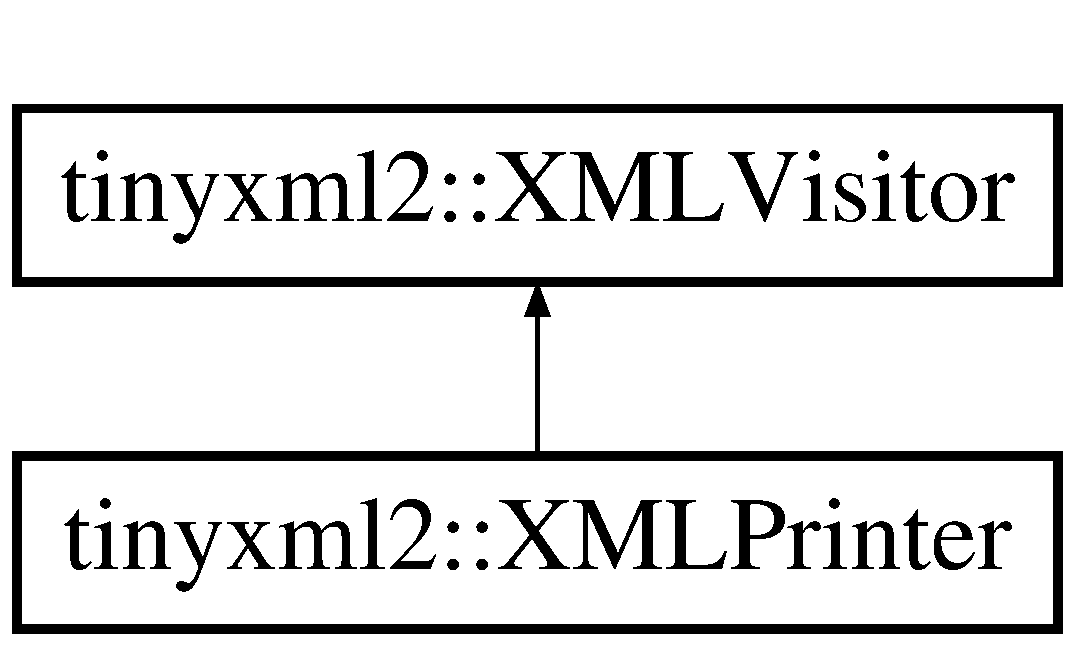
\includegraphics[height=2.000000cm]{classtinyxml2_1_1_x_m_l_printer}
\end{center}
\end{figure}
\subsection*{Public Member Functions}
\begin{DoxyCompactItemize}
\item 
\hyperlink{classtinyxml2_1_1_x_m_l_printer_aa6d3841c069085f5b8a27bc7103c04f7}{X\-M\-L\-Printer} (F\-I\-L\-E $\ast$file=0, bool compact=false, int depth=0)
\item 
virtual \hyperlink{classtinyxml2_1_1_x_m_l_printer_af4caefa48ea6436898fb1807de8d14c0}{$\sim$\-X\-M\-L\-Printer} ()
\item 
void \hyperlink{classtinyxml2_1_1_x_m_l_printer_a178c608ce8476043d5d6513819cde903}{Push\-Header} (bool write\-B\-O\-M, bool write\-Declaration)
\item 
void \hyperlink{classtinyxml2_1_1_x_m_l_printer_a5f397c5502c545c65fe9a8f46f4acebd}{Open\-Element} (const char $\ast$name, bool compact\-Mode)
\item 
void \hyperlink{classtinyxml2_1_1_x_m_l_printer_a9a4e2c9348b42e147629d5a99f4af3f0}{Push\-Attribute} (const char $\ast$name, const char $\ast$value)
\begin{DoxyCompactList}\small\item\em If streaming, add an attribute to an open element. \end{DoxyCompactList}\item 
void \hyperlink{classtinyxml2_1_1_x_m_l_printer_a69120c82088597372d28d0a98f2ee7a1}{Push\-Attribute} (const char $\ast$name, int value)
\item 
void \hyperlink{classtinyxml2_1_1_x_m_l_printer_aa41039e51990aaf5342f3e0575a692c4}{Push\-Attribute} (const char $\ast$name, unsigned value)
\item 
void \hyperlink{classtinyxml2_1_1_x_m_l_printer_a51f7950d7b7a19f0d3a0d549a318d45f}{Push\-Attribute} (const char $\ast$name, bool value)
\item 
void \hyperlink{classtinyxml2_1_1_x_m_l_printer_a1714867af40e68ca404c3e84b6cac2a6}{Push\-Attribute} (const char $\ast$name, double value)
\item 
virtual void \hyperlink{classtinyxml2_1_1_x_m_l_printer_adb8e885f55212bf36e9c602211e3068c}{Close\-Element} (bool compact\-Mode)
\begin{DoxyCompactList}\small\item\em If streaming, close the Element. \end{DoxyCompactList}\item 
void \hyperlink{classtinyxml2_1_1_x_m_l_printer_a1cc16a9362df4332012cb13cff6441b3}{Push\-Text} (const char $\ast$text, bool cdata=false)
\begin{DoxyCompactList}\small\item\em Add a text node. \end{DoxyCompactList}\item 
void \hyperlink{classtinyxml2_1_1_x_m_l_printer_a3e0d4d78de25d4cf081009e1431cea7e}{Push\-Text} (int value)
\begin{DoxyCompactList}\small\item\em Add a text node from an integer. \end{DoxyCompactList}\item 
void \hyperlink{classtinyxml2_1_1_x_m_l_printer_a661fb50e7e0a4918d2d259cb0fae647e}{Push\-Text} (unsigned value)
\begin{DoxyCompactList}\small\item\em Add a text node from an unsigned. \end{DoxyCompactList}\item 
void \hyperlink{classtinyxml2_1_1_x_m_l_printer_a4390e5fa1ed05189a8686647345ab29f}{Push\-Text} (bool value)
\begin{DoxyCompactList}\small\item\em Add a text node from a bool. \end{DoxyCompactList}\item 
void \hyperlink{classtinyxml2_1_1_x_m_l_printer_a1dbb1390e829d0673af66b9cd1928bd7}{Push\-Text} (float value)
\begin{DoxyCompactList}\small\item\em Add a text node from a float. \end{DoxyCompactList}\item 
void \hyperlink{classtinyxml2_1_1_x_m_l_printer_aa715302dfc09473c77c853cbd5431965}{Push\-Text} (double value)
\begin{DoxyCompactList}\small\item\em Add a text node from a double. \end{DoxyCompactList}\item 
void \hyperlink{classtinyxml2_1_1_x_m_l_printer_afc8416814219591c2fd5656e0c233140}{Push\-Comment} (const char $\ast$comment)
\begin{DoxyCompactList}\small\item\em Add a comment. \end{DoxyCompactList}\item 
void \hyperlink{classtinyxml2_1_1_x_m_l_printer_a2fe3565e262594efc6c0276723c83fe7}{Push\-Declaration} (const char $\ast$value)
\item 
void \hyperlink{classtinyxml2_1_1_x_m_l_printer_ab1efc6d1548505e9984185f58f54b713}{Push\-Unknown} (const char $\ast$value)
\item 
virtual bool \hyperlink{classtinyxml2_1_1_x_m_l_printer_a9aa1de11a55a07db55a90fde37d7afad}{Visit\-Enter} (const \hyperlink{classtinyxml2_1_1_x_m_l_document}{X\-M\-L\-Document} \&)
\begin{DoxyCompactList}\small\item\em Visit a document. \end{DoxyCompactList}\item 
virtual bool \hyperlink{classtinyxml2_1_1_x_m_l_printer_a15fc1f2b922f540917dcf52808737b29}{Visit\-Exit} (const \hyperlink{classtinyxml2_1_1_x_m_l_document}{X\-M\-L\-Document} \&)
\begin{DoxyCompactList}\small\item\em Visit a document. \end{DoxyCompactList}\item 
virtual bool \hyperlink{classtinyxml2_1_1_x_m_l_printer_a169b2509d8eabb70811b2bb8cfd1f5d1}{Visit\-Enter} (const \hyperlink{classtinyxml2_1_1_x_m_l_element}{X\-M\-L\-Element} \&element, const \hyperlink{classtinyxml2_1_1_x_m_l_attribute}{X\-M\-L\-Attribute} $\ast$attribute)
\begin{DoxyCompactList}\small\item\em Visit an element. \end{DoxyCompactList}\item 
virtual bool \hyperlink{classtinyxml2_1_1_x_m_l_printer_a2edd48405971a88951c71c9df86a2f50}{Visit\-Exit} (const \hyperlink{classtinyxml2_1_1_x_m_l_element}{X\-M\-L\-Element} \&element)
\begin{DoxyCompactList}\small\item\em Visit an element. \end{DoxyCompactList}\item 
virtual bool \hyperlink{classtinyxml2_1_1_x_m_l_printer_adc0e42b4f6fcb90a95630c79575d030b}{Visit} (const \hyperlink{classtinyxml2_1_1_x_m_l_text}{X\-M\-L\-Text} \&text)
\begin{DoxyCompactList}\small\item\em Visit a text node. \end{DoxyCompactList}\item 
virtual bool \hyperlink{classtinyxml2_1_1_x_m_l_printer_aa294c5c01af0ebb9114902456e4cb53c}{Visit} (const \hyperlink{classtinyxml2_1_1_x_m_l_comment}{X\-M\-L\-Comment} \&comment)
\begin{DoxyCompactList}\small\item\em Visit a comment node. \end{DoxyCompactList}\item 
virtual bool \hyperlink{classtinyxml2_1_1_x_m_l_printer_acfc625b2549304b9c7eb85ebd5c5eb39}{Visit} (const \hyperlink{classtinyxml2_1_1_x_m_l_declaration}{X\-M\-L\-Declaration} \&declaration)
\begin{DoxyCompactList}\small\item\em Visit a declaration. \end{DoxyCompactList}\item 
virtual bool \hyperlink{classtinyxml2_1_1_x_m_l_printer_ab8af5455bbf9e4be2663e6642fcd7e32}{Visit} (const \hyperlink{classtinyxml2_1_1_x_m_l_unknown}{X\-M\-L\-Unknown} \&unknown)
\begin{DoxyCompactList}\small\item\em Visit an unknown node. \end{DoxyCompactList}\item 
const char $\ast$ \hyperlink{classtinyxml2_1_1_x_m_l_printer_a4a1b788e11b540921ec50687cd2b24a9}{C\-Str} () const 
\item 
int \hyperlink{classtinyxml2_1_1_x_m_l_printer_a02c3c5f8c6c007dcbaf10595d9e22bf0}{C\-Str\-Size} () const 
\item 
void \hyperlink{classtinyxml2_1_1_x_m_l_printer_a216157765b7267bf389975b1cbf9a909}{Clear\-Buffer} ()
\end{DoxyCompactItemize}
\subsection*{Protected Member Functions}
\begin{DoxyCompactItemize}
\item 
virtual bool \hyperlink{classtinyxml2_1_1_x_m_l_printer_a38e1ed5a779bdf63eda9e808f7a6de66}{Compact\-Mode} (const \hyperlink{classtinyxml2_1_1_x_m_l_element}{X\-M\-L\-Element} \&)
\item 
virtual void \hyperlink{classtinyxml2_1_1_x_m_l_printer_a1c4b2ccbe4fdb316d54f5a93f3559260}{Print\-Space} (int depth)
\item 
void \hyperlink{classtinyxml2_1_1_x_m_l_printer_ab30210a7f32e45634e7a45137bf6fdf6}{Print} (const char $\ast$format,...)
\item 
void \hyperlink{classtinyxml2_1_1_x_m_l_printer_a70ac2010150c8551773ffb2f96fef353}{Seal\-Element} ()
\end{DoxyCompactItemize}
\subsection*{Protected Attributes}
\begin{DoxyCompactItemize}
\item 
bool \hyperlink{classtinyxml2_1_1_x_m_l_printer_ac07169d58b465214a2b1fa306e617c26}{\-\_\-element\-Just\-Opened}
\item 
\hyperlink{classtinyxml2_1_1_dyn_array}{Dyn\-Array}$<$ const char $\ast$, 10 $>$ \hyperlink{classtinyxml2_1_1_x_m_l_printer_a99d59e67e084714541bee3ae43884bef}{\-\_\-stack}
\end{DoxyCompactItemize}
\subsection*{Private Types}
\begin{DoxyCompactItemize}
\item 
enum \{ \hyperlink{classtinyxml2_1_1_x_m_l_printer_abd08e8da55b22d059d0484c53db1fae8a2ddc02813235fe451809606959166db5}{E\-N\-T\-I\-T\-Y\-\_\-\-R\-A\-N\-G\-E} = 64, 
\hyperlink{classtinyxml2_1_1_x_m_l_printer_abd08e8da55b22d059d0484c53db1fae8a1f747a8fb39ceb2e711c3798058fb632}{B\-U\-F\-\_\-\-S\-I\-Z\-E} = 200
 \}
\end{DoxyCompactItemize}
\subsection*{Private Member Functions}
\begin{DoxyCompactItemize}
\item 
void \hyperlink{classtinyxml2_1_1_x_m_l_printer_a5495e504053f63f2c4d603327314fa91}{Print\-String} (const char $\ast$, bool restricted\-Entity\-Set)
\end{DoxyCompactItemize}
\subsection*{Private Attributes}
\begin{DoxyCompactItemize}
\item 
bool \hyperlink{classtinyxml2_1_1_x_m_l_printer_abbd7ac45d97ae5eceec12d6c058119f9}{\-\_\-first\-Element}
\item 
F\-I\-L\-E $\ast$ \hyperlink{classtinyxml2_1_1_x_m_l_printer_a79d91decf17990f7ce18b592f3fdf44e}{\-\_\-fp}
\item 
int \hyperlink{classtinyxml2_1_1_x_m_l_printer_a19cd59a9dbe4b666264803fb91ac8ec1}{\-\_\-depth}
\item 
int \hyperlink{classtinyxml2_1_1_x_m_l_printer_a3c5a442e57131faefde97188e92144f3}{\-\_\-text\-Depth}
\item 
bool \hyperlink{classtinyxml2_1_1_x_m_l_printer_a3e27c4b4fe791a96e4e139b5034e190b}{\-\_\-process\-Entities}
\item 
bool \hyperlink{classtinyxml2_1_1_x_m_l_printer_a7bc067aa3f0dcee68e4ac75e19117bd0}{\-\_\-compact\-Mode}
\item 
bool \hyperlink{classtinyxml2_1_1_x_m_l_printer_a334eb34c43f21daebef9341b4768c275}{\-\_\-entity\-Flag} \mbox{[}\hyperlink{classtinyxml2_1_1_x_m_l_printer_abd08e8da55b22d059d0484c53db1fae8a2ddc02813235fe451809606959166db5}{E\-N\-T\-I\-T\-Y\-\_\-\-R\-A\-N\-G\-E}\mbox{]}
\item 
bool \hyperlink{classtinyxml2_1_1_x_m_l_printer_a5df242509d42ae1c9128924121ebe093}{\-\_\-restricted\-Entity\-Flag} \mbox{[}\hyperlink{classtinyxml2_1_1_x_m_l_printer_abd08e8da55b22d059d0484c53db1fae8a2ddc02813235fe451809606959166db5}{E\-N\-T\-I\-T\-Y\-\_\-\-R\-A\-N\-G\-E}\mbox{]}
\item 
\hyperlink{classtinyxml2_1_1_dyn_array}{Dyn\-Array}$<$ char, 20 $>$ \hyperlink{classtinyxml2_1_1_x_m_l_printer_a19fca2e934576a892fefe2f602874d59}{\-\_\-buffer}
\end{DoxyCompactItemize}


\subsection{Detailed Description}
Printing functionality. The \hyperlink{classtinyxml2_1_1_x_m_l_printer}{X\-M\-L\-Printer} gives you more options than the \hyperlink{classtinyxml2_1_1_x_m_l_document_a686ea28672c0e0c60383ec28148c1ac0}{X\-M\-L\-Document\-::\-Print()} method.

It can\-:
\begin{DoxyEnumerate}
\item Print to memory.
\item Print to a file you provide.
\item Print X\-M\-L without a \hyperlink{classtinyxml2_1_1_x_m_l_document}{X\-M\-L\-Document}.
\end{DoxyEnumerate}

Print to Memory

\begin{DoxyVerb}XMLPrinter printer;
doc.Print( &printer );
SomeFunction( printer.CStr() );
\end{DoxyVerb}


Print to a File

You provide the file pointer. \begin{DoxyVerb}XMLPrinter printer( fp );
doc.Print( &printer );
\end{DoxyVerb}


Print without a \hyperlink{classtinyxml2_1_1_x_m_l_document}{X\-M\-L\-Document}

When loading, an X\-M\-L parser is very useful. However, sometimes when saving, it just gets in the way. The code is often set up for streaming, and constructing the D\-O\-M is just overhead.

The Printer supports the streaming case. The following code prints out a trivially simple X\-M\-L file without ever creating an X\-M\-L document.

\begin{DoxyVerb}XMLPrinter printer( fp );
printer.OpenElement( "foo" );
printer.PushAttribute( "foo", "bar" );
printer.CloseElement();
\end{DoxyVerb}
 

\subsection{Member Enumeration Documentation}
\hypertarget{classtinyxml2_1_1_x_m_l_printer_abd08e8da55b22d059d0484c53db1fae8}{\subsubsection[{anonymous enum}]{\setlength{\rightskip}{0pt plus 5cm}anonymous enum\hspace{0.3cm}{\ttfamily [private]}}}\label{classtinyxml2_1_1_x_m_l_printer_abd08e8da55b22d059d0484c53db1fae8}
\begin{Desc}
\item[Enumerator]\par
\begin{description}
\index{E\-N\-T\-I\-T\-Y\-\_\-\-R\-A\-N\-G\-E@{E\-N\-T\-I\-T\-Y\-\_\-\-R\-A\-N\-G\-E}!tinyxml2\-::\-X\-M\-L\-Printer@{tinyxml2\-::\-X\-M\-L\-Printer}}\index{tinyxml2\-::\-X\-M\-L\-Printer@{tinyxml2\-::\-X\-M\-L\-Printer}!E\-N\-T\-I\-T\-Y\-\_\-\-R\-A\-N\-G\-E@{E\-N\-T\-I\-T\-Y\-\_\-\-R\-A\-N\-G\-E}}\item[{\em 
\hypertarget{classtinyxml2_1_1_x_m_l_printer_abd08e8da55b22d059d0484c53db1fae8a2ddc02813235fe451809606959166db5}{E\-N\-T\-I\-T\-Y\-\_\-\-R\-A\-N\-G\-E}\label{classtinyxml2_1_1_x_m_l_printer_abd08e8da55b22d059d0484c53db1fae8a2ddc02813235fe451809606959166db5}
}]\index{B\-U\-F\-\_\-\-S\-I\-Z\-E@{B\-U\-F\-\_\-\-S\-I\-Z\-E}!tinyxml2\-::\-X\-M\-L\-Printer@{tinyxml2\-::\-X\-M\-L\-Printer}}\index{tinyxml2\-::\-X\-M\-L\-Printer@{tinyxml2\-::\-X\-M\-L\-Printer}!B\-U\-F\-\_\-\-S\-I\-Z\-E@{B\-U\-F\-\_\-\-S\-I\-Z\-E}}\item[{\em 
\hypertarget{classtinyxml2_1_1_x_m_l_printer_abd08e8da55b22d059d0484c53db1fae8a1f747a8fb39ceb2e711c3798058fb632}{B\-U\-F\-\_\-\-S\-I\-Z\-E}\label{classtinyxml2_1_1_x_m_l_printer_abd08e8da55b22d059d0484c53db1fae8a1f747a8fb39ceb2e711c3798058fb632}
}]\end{description}
\end{Desc}


\subsection{Constructor \& Destructor Documentation}
\hypertarget{classtinyxml2_1_1_x_m_l_printer_aa6d3841c069085f5b8a27bc7103c04f7}{\index{tinyxml2\-::\-X\-M\-L\-Printer@{tinyxml2\-::\-X\-M\-L\-Printer}!X\-M\-L\-Printer@{X\-M\-L\-Printer}}
\index{X\-M\-L\-Printer@{X\-M\-L\-Printer}!tinyxml2::XMLPrinter@{tinyxml2\-::\-X\-M\-L\-Printer}}
\subsubsection[{X\-M\-L\-Printer}]{\setlength{\rightskip}{0pt plus 5cm}tinyxml2\-::\-X\-M\-L\-Printer\-::\-X\-M\-L\-Printer (
\begin{DoxyParamCaption}
\item[{F\-I\-L\-E $\ast$}]{file = {\ttfamily 0}, }
\item[{bool}]{compact = {\ttfamily false}, }
\item[{int}]{depth = {\ttfamily 0}}
\end{DoxyParamCaption}
)}}\label{classtinyxml2_1_1_x_m_l_printer_aa6d3841c069085f5b8a27bc7103c04f7}
Construct the printer. If the F\-I\-L\-E$\ast$ is specified, this will print to the F\-I\-L\-E. Else it will print to memory, and the result is available in \hyperlink{classtinyxml2_1_1_x_m_l_printer_a4a1b788e11b540921ec50687cd2b24a9}{C\-Str()}. If 'compact' is set to true, then output is created with only required whitespace and newlines. \hypertarget{classtinyxml2_1_1_x_m_l_printer_af4caefa48ea6436898fb1807de8d14c0}{\index{tinyxml2\-::\-X\-M\-L\-Printer@{tinyxml2\-::\-X\-M\-L\-Printer}!$\sim$\-X\-M\-L\-Printer@{$\sim$\-X\-M\-L\-Printer}}
\index{$\sim$\-X\-M\-L\-Printer@{$\sim$\-X\-M\-L\-Printer}!tinyxml2::XMLPrinter@{tinyxml2\-::\-X\-M\-L\-Printer}}
\subsubsection[{$\sim$\-X\-M\-L\-Printer}]{\setlength{\rightskip}{0pt plus 5cm}virtual tinyxml2\-::\-X\-M\-L\-Printer\-::$\sim$\-X\-M\-L\-Printer (
\begin{DoxyParamCaption}
{}
\end{DoxyParamCaption}
)\hspace{0.3cm}{\ttfamily [inline]}, {\ttfamily [virtual]}}}\label{classtinyxml2_1_1_x_m_l_printer_af4caefa48ea6436898fb1807de8d14c0}


\subsection{Member Function Documentation}
\hypertarget{classtinyxml2_1_1_x_m_l_printer_a216157765b7267bf389975b1cbf9a909}{\index{tinyxml2\-::\-X\-M\-L\-Printer@{tinyxml2\-::\-X\-M\-L\-Printer}!Clear\-Buffer@{Clear\-Buffer}}
\index{Clear\-Buffer@{Clear\-Buffer}!tinyxml2::XMLPrinter@{tinyxml2\-::\-X\-M\-L\-Printer}}
\subsubsection[{Clear\-Buffer}]{\setlength{\rightskip}{0pt plus 5cm}void tinyxml2\-::\-X\-M\-L\-Printer\-::\-Clear\-Buffer (
\begin{DoxyParamCaption}
{}
\end{DoxyParamCaption}
)\hspace{0.3cm}{\ttfamily [inline]}}}\label{classtinyxml2_1_1_x_m_l_printer_a216157765b7267bf389975b1cbf9a909}
If in print to memory mode, reset the buffer to the beginning. \hypertarget{classtinyxml2_1_1_x_m_l_printer_adb8e885f55212bf36e9c602211e3068c}{\index{tinyxml2\-::\-X\-M\-L\-Printer@{tinyxml2\-::\-X\-M\-L\-Printer}!Close\-Element@{Close\-Element}}
\index{Close\-Element@{Close\-Element}!tinyxml2::XMLPrinter@{tinyxml2\-::\-X\-M\-L\-Printer}}
\subsubsection[{Close\-Element}]{\setlength{\rightskip}{0pt plus 5cm}void tinyxml2\-::\-X\-M\-L\-Printer\-::\-Close\-Element (
\begin{DoxyParamCaption}
\item[{bool}]{compact\-Mode}
\end{DoxyParamCaption}
)\hspace{0.3cm}{\ttfamily [virtual]}}}\label{classtinyxml2_1_1_x_m_l_printer_adb8e885f55212bf36e9c602211e3068c}


If streaming, close the Element. 

\hypertarget{classtinyxml2_1_1_x_m_l_printer_a38e1ed5a779bdf63eda9e808f7a6de66}{\index{tinyxml2\-::\-X\-M\-L\-Printer@{tinyxml2\-::\-X\-M\-L\-Printer}!Compact\-Mode@{Compact\-Mode}}
\index{Compact\-Mode@{Compact\-Mode}!tinyxml2::XMLPrinter@{tinyxml2\-::\-X\-M\-L\-Printer}}
\subsubsection[{Compact\-Mode}]{\setlength{\rightskip}{0pt plus 5cm}virtual bool tinyxml2\-::\-X\-M\-L\-Printer\-::\-Compact\-Mode (
\begin{DoxyParamCaption}
\item[{const {\bf X\-M\-L\-Element} \&}]{}
\end{DoxyParamCaption}
)\hspace{0.3cm}{\ttfamily [inline]}, {\ttfamily [protected]}, {\ttfamily [virtual]}}}\label{classtinyxml2_1_1_x_m_l_printer_a38e1ed5a779bdf63eda9e808f7a6de66}
\hypertarget{classtinyxml2_1_1_x_m_l_printer_a4a1b788e11b540921ec50687cd2b24a9}{\index{tinyxml2\-::\-X\-M\-L\-Printer@{tinyxml2\-::\-X\-M\-L\-Printer}!C\-Str@{C\-Str}}
\index{C\-Str@{C\-Str}!tinyxml2::XMLPrinter@{tinyxml2\-::\-X\-M\-L\-Printer}}
\subsubsection[{C\-Str}]{\setlength{\rightskip}{0pt plus 5cm}const char$\ast$ tinyxml2\-::\-X\-M\-L\-Printer\-::\-C\-Str (
\begin{DoxyParamCaption}
{}
\end{DoxyParamCaption}
) const\hspace{0.3cm}{\ttfamily [inline]}}}\label{classtinyxml2_1_1_x_m_l_printer_a4a1b788e11b540921ec50687cd2b24a9}
If in print to memory mode, return a pointer to the X\-M\-L file in memory. \hypertarget{classtinyxml2_1_1_x_m_l_printer_a02c3c5f8c6c007dcbaf10595d9e22bf0}{\index{tinyxml2\-::\-X\-M\-L\-Printer@{tinyxml2\-::\-X\-M\-L\-Printer}!C\-Str\-Size@{C\-Str\-Size}}
\index{C\-Str\-Size@{C\-Str\-Size}!tinyxml2::XMLPrinter@{tinyxml2\-::\-X\-M\-L\-Printer}}
\subsubsection[{C\-Str\-Size}]{\setlength{\rightskip}{0pt plus 5cm}int tinyxml2\-::\-X\-M\-L\-Printer\-::\-C\-Str\-Size (
\begin{DoxyParamCaption}
{}
\end{DoxyParamCaption}
) const\hspace{0.3cm}{\ttfamily [inline]}}}\label{classtinyxml2_1_1_x_m_l_printer_a02c3c5f8c6c007dcbaf10595d9e22bf0}
If in print to memory mode, return the size of the X\-M\-L file in memory. (Note the size returned includes the terminating null.) \hypertarget{classtinyxml2_1_1_x_m_l_printer_a5f397c5502c545c65fe9a8f46f4acebd}{\index{tinyxml2\-::\-X\-M\-L\-Printer@{tinyxml2\-::\-X\-M\-L\-Printer}!Open\-Element@{Open\-Element}}
\index{Open\-Element@{Open\-Element}!tinyxml2::XMLPrinter@{tinyxml2\-::\-X\-M\-L\-Printer}}
\subsubsection[{Open\-Element}]{\setlength{\rightskip}{0pt plus 5cm}void tinyxml2\-::\-X\-M\-L\-Printer\-::\-Open\-Element (
\begin{DoxyParamCaption}
\item[{const char $\ast$}]{name, }
\item[{bool}]{compact\-Mode}
\end{DoxyParamCaption}
)}}\label{classtinyxml2_1_1_x_m_l_printer_a5f397c5502c545c65fe9a8f46f4acebd}
If streaming, start writing an element. The element must be closed with \hyperlink{classtinyxml2_1_1_x_m_l_printer_adb8e885f55212bf36e9c602211e3068c}{Close\-Element()} \hypertarget{classtinyxml2_1_1_x_m_l_printer_ab30210a7f32e45634e7a45137bf6fdf6}{\index{tinyxml2\-::\-X\-M\-L\-Printer@{tinyxml2\-::\-X\-M\-L\-Printer}!Print@{Print}}
\index{Print@{Print}!tinyxml2::XMLPrinter@{tinyxml2\-::\-X\-M\-L\-Printer}}
\subsubsection[{Print}]{\setlength{\rightskip}{0pt plus 5cm}void tinyxml2\-::\-X\-M\-L\-Printer\-::\-Print (
\begin{DoxyParamCaption}
\item[{const char $\ast$}]{format, }
\item[{}]{...}
\end{DoxyParamCaption}
)\hspace{0.3cm}{\ttfamily [protected]}}}\label{classtinyxml2_1_1_x_m_l_printer_ab30210a7f32e45634e7a45137bf6fdf6}
\hypertarget{classtinyxml2_1_1_x_m_l_printer_a1c4b2ccbe4fdb316d54f5a93f3559260}{\index{tinyxml2\-::\-X\-M\-L\-Printer@{tinyxml2\-::\-X\-M\-L\-Printer}!Print\-Space@{Print\-Space}}
\index{Print\-Space@{Print\-Space}!tinyxml2::XMLPrinter@{tinyxml2\-::\-X\-M\-L\-Printer}}
\subsubsection[{Print\-Space}]{\setlength{\rightskip}{0pt plus 5cm}void tinyxml2\-::\-X\-M\-L\-Printer\-::\-Print\-Space (
\begin{DoxyParamCaption}
\item[{int}]{depth}
\end{DoxyParamCaption}
)\hspace{0.3cm}{\ttfamily [protected]}, {\ttfamily [virtual]}}}\label{classtinyxml2_1_1_x_m_l_printer_a1c4b2ccbe4fdb316d54f5a93f3559260}
Prints out the space before an element. You may override to change the space and tabs used. A \hyperlink{classtinyxml2_1_1_x_m_l_printer_a1c4b2ccbe4fdb316d54f5a93f3559260}{Print\-Space()} override should call \hyperlink{classtinyxml2_1_1_x_m_l_printer_ab30210a7f32e45634e7a45137bf6fdf6}{Print()}. \hypertarget{classtinyxml2_1_1_x_m_l_printer_a5495e504053f63f2c4d603327314fa91}{\index{tinyxml2\-::\-X\-M\-L\-Printer@{tinyxml2\-::\-X\-M\-L\-Printer}!Print\-String@{Print\-String}}
\index{Print\-String@{Print\-String}!tinyxml2::XMLPrinter@{tinyxml2\-::\-X\-M\-L\-Printer}}
\subsubsection[{Print\-String}]{\setlength{\rightskip}{0pt plus 5cm}void tinyxml2\-::\-X\-M\-L\-Printer\-::\-Print\-String (
\begin{DoxyParamCaption}
\item[{const char $\ast$}]{p, }
\item[{bool}]{restricted\-Entity\-Set}
\end{DoxyParamCaption}
)\hspace{0.3cm}{\ttfamily [private]}}}\label{classtinyxml2_1_1_x_m_l_printer_a5495e504053f63f2c4d603327314fa91}
\hypertarget{classtinyxml2_1_1_x_m_l_printer_a9a4e2c9348b42e147629d5a99f4af3f0}{\index{tinyxml2\-::\-X\-M\-L\-Printer@{tinyxml2\-::\-X\-M\-L\-Printer}!Push\-Attribute@{Push\-Attribute}}
\index{Push\-Attribute@{Push\-Attribute}!tinyxml2::XMLPrinter@{tinyxml2\-::\-X\-M\-L\-Printer}}
\subsubsection[{Push\-Attribute}]{\setlength{\rightskip}{0pt plus 5cm}void tinyxml2\-::\-X\-M\-L\-Printer\-::\-Push\-Attribute (
\begin{DoxyParamCaption}
\item[{const char $\ast$}]{name, }
\item[{const char $\ast$}]{value}
\end{DoxyParamCaption}
)}}\label{classtinyxml2_1_1_x_m_l_printer_a9a4e2c9348b42e147629d5a99f4af3f0}


If streaming, add an attribute to an open element. 

\hypertarget{classtinyxml2_1_1_x_m_l_printer_a69120c82088597372d28d0a98f2ee7a1}{\index{tinyxml2\-::\-X\-M\-L\-Printer@{tinyxml2\-::\-X\-M\-L\-Printer}!Push\-Attribute@{Push\-Attribute}}
\index{Push\-Attribute@{Push\-Attribute}!tinyxml2::XMLPrinter@{tinyxml2\-::\-X\-M\-L\-Printer}}
\subsubsection[{Push\-Attribute}]{\setlength{\rightskip}{0pt plus 5cm}void tinyxml2\-::\-X\-M\-L\-Printer\-::\-Push\-Attribute (
\begin{DoxyParamCaption}
\item[{const char $\ast$}]{name, }
\item[{int}]{value}
\end{DoxyParamCaption}
)}}\label{classtinyxml2_1_1_x_m_l_printer_a69120c82088597372d28d0a98f2ee7a1}
\hypertarget{classtinyxml2_1_1_x_m_l_printer_aa41039e51990aaf5342f3e0575a692c4}{\index{tinyxml2\-::\-X\-M\-L\-Printer@{tinyxml2\-::\-X\-M\-L\-Printer}!Push\-Attribute@{Push\-Attribute}}
\index{Push\-Attribute@{Push\-Attribute}!tinyxml2::XMLPrinter@{tinyxml2\-::\-X\-M\-L\-Printer}}
\subsubsection[{Push\-Attribute}]{\setlength{\rightskip}{0pt plus 5cm}void tinyxml2\-::\-X\-M\-L\-Printer\-::\-Push\-Attribute (
\begin{DoxyParamCaption}
\item[{const char $\ast$}]{name, }
\item[{unsigned}]{value}
\end{DoxyParamCaption}
)}}\label{classtinyxml2_1_1_x_m_l_printer_aa41039e51990aaf5342f3e0575a692c4}
\hypertarget{classtinyxml2_1_1_x_m_l_printer_a51f7950d7b7a19f0d3a0d549a318d45f}{\index{tinyxml2\-::\-X\-M\-L\-Printer@{tinyxml2\-::\-X\-M\-L\-Printer}!Push\-Attribute@{Push\-Attribute}}
\index{Push\-Attribute@{Push\-Attribute}!tinyxml2::XMLPrinter@{tinyxml2\-::\-X\-M\-L\-Printer}}
\subsubsection[{Push\-Attribute}]{\setlength{\rightskip}{0pt plus 5cm}void tinyxml2\-::\-X\-M\-L\-Printer\-::\-Push\-Attribute (
\begin{DoxyParamCaption}
\item[{const char $\ast$}]{name, }
\item[{bool}]{value}
\end{DoxyParamCaption}
)}}\label{classtinyxml2_1_1_x_m_l_printer_a51f7950d7b7a19f0d3a0d549a318d45f}
\hypertarget{classtinyxml2_1_1_x_m_l_printer_a1714867af40e68ca404c3e84b6cac2a6}{\index{tinyxml2\-::\-X\-M\-L\-Printer@{tinyxml2\-::\-X\-M\-L\-Printer}!Push\-Attribute@{Push\-Attribute}}
\index{Push\-Attribute@{Push\-Attribute}!tinyxml2::XMLPrinter@{tinyxml2\-::\-X\-M\-L\-Printer}}
\subsubsection[{Push\-Attribute}]{\setlength{\rightskip}{0pt plus 5cm}void tinyxml2\-::\-X\-M\-L\-Printer\-::\-Push\-Attribute (
\begin{DoxyParamCaption}
\item[{const char $\ast$}]{name, }
\item[{double}]{value}
\end{DoxyParamCaption}
)}}\label{classtinyxml2_1_1_x_m_l_printer_a1714867af40e68ca404c3e84b6cac2a6}
\hypertarget{classtinyxml2_1_1_x_m_l_printer_afc8416814219591c2fd5656e0c233140}{\index{tinyxml2\-::\-X\-M\-L\-Printer@{tinyxml2\-::\-X\-M\-L\-Printer}!Push\-Comment@{Push\-Comment}}
\index{Push\-Comment@{Push\-Comment}!tinyxml2::XMLPrinter@{tinyxml2\-::\-X\-M\-L\-Printer}}
\subsubsection[{Push\-Comment}]{\setlength{\rightskip}{0pt plus 5cm}void tinyxml2\-::\-X\-M\-L\-Printer\-::\-Push\-Comment (
\begin{DoxyParamCaption}
\item[{const char $\ast$}]{comment}
\end{DoxyParamCaption}
)}}\label{classtinyxml2_1_1_x_m_l_printer_afc8416814219591c2fd5656e0c233140}


Add a comment. 

\hypertarget{classtinyxml2_1_1_x_m_l_printer_a2fe3565e262594efc6c0276723c83fe7}{\index{tinyxml2\-::\-X\-M\-L\-Printer@{tinyxml2\-::\-X\-M\-L\-Printer}!Push\-Declaration@{Push\-Declaration}}
\index{Push\-Declaration@{Push\-Declaration}!tinyxml2::XMLPrinter@{tinyxml2\-::\-X\-M\-L\-Printer}}
\subsubsection[{Push\-Declaration}]{\setlength{\rightskip}{0pt plus 5cm}void tinyxml2\-::\-X\-M\-L\-Printer\-::\-Push\-Declaration (
\begin{DoxyParamCaption}
\item[{const char $\ast$}]{value}
\end{DoxyParamCaption}
)}}\label{classtinyxml2_1_1_x_m_l_printer_a2fe3565e262594efc6c0276723c83fe7}
\hypertarget{classtinyxml2_1_1_x_m_l_printer_a178c608ce8476043d5d6513819cde903}{\index{tinyxml2\-::\-X\-M\-L\-Printer@{tinyxml2\-::\-X\-M\-L\-Printer}!Push\-Header@{Push\-Header}}
\index{Push\-Header@{Push\-Header}!tinyxml2::XMLPrinter@{tinyxml2\-::\-X\-M\-L\-Printer}}
\subsubsection[{Push\-Header}]{\setlength{\rightskip}{0pt plus 5cm}void tinyxml2\-::\-X\-M\-L\-Printer\-::\-Push\-Header (
\begin{DoxyParamCaption}
\item[{bool}]{write\-B\-O\-M, }
\item[{bool}]{write\-Declaration}
\end{DoxyParamCaption}
)}}\label{classtinyxml2_1_1_x_m_l_printer_a178c608ce8476043d5d6513819cde903}
If streaming, write the B\-O\-M and declaration. \hypertarget{classtinyxml2_1_1_x_m_l_printer_a1cc16a9362df4332012cb13cff6441b3}{\index{tinyxml2\-::\-X\-M\-L\-Printer@{tinyxml2\-::\-X\-M\-L\-Printer}!Push\-Text@{Push\-Text}}
\index{Push\-Text@{Push\-Text}!tinyxml2::XMLPrinter@{tinyxml2\-::\-X\-M\-L\-Printer}}
\subsubsection[{Push\-Text}]{\setlength{\rightskip}{0pt plus 5cm}void tinyxml2\-::\-X\-M\-L\-Printer\-::\-Push\-Text (
\begin{DoxyParamCaption}
\item[{const char $\ast$}]{text, }
\item[{bool}]{cdata = {\ttfamily false}}
\end{DoxyParamCaption}
)}}\label{classtinyxml2_1_1_x_m_l_printer_a1cc16a9362df4332012cb13cff6441b3}


Add a text node. 

\hypertarget{classtinyxml2_1_1_x_m_l_printer_a3e0d4d78de25d4cf081009e1431cea7e}{\index{tinyxml2\-::\-X\-M\-L\-Printer@{tinyxml2\-::\-X\-M\-L\-Printer}!Push\-Text@{Push\-Text}}
\index{Push\-Text@{Push\-Text}!tinyxml2::XMLPrinter@{tinyxml2\-::\-X\-M\-L\-Printer}}
\subsubsection[{Push\-Text}]{\setlength{\rightskip}{0pt plus 5cm}void tinyxml2\-::\-X\-M\-L\-Printer\-::\-Push\-Text (
\begin{DoxyParamCaption}
\item[{int}]{value}
\end{DoxyParamCaption}
)}}\label{classtinyxml2_1_1_x_m_l_printer_a3e0d4d78de25d4cf081009e1431cea7e}


Add a text node from an integer. 

\hypertarget{classtinyxml2_1_1_x_m_l_printer_a661fb50e7e0a4918d2d259cb0fae647e}{\index{tinyxml2\-::\-X\-M\-L\-Printer@{tinyxml2\-::\-X\-M\-L\-Printer}!Push\-Text@{Push\-Text}}
\index{Push\-Text@{Push\-Text}!tinyxml2::XMLPrinter@{tinyxml2\-::\-X\-M\-L\-Printer}}
\subsubsection[{Push\-Text}]{\setlength{\rightskip}{0pt plus 5cm}void tinyxml2\-::\-X\-M\-L\-Printer\-::\-Push\-Text (
\begin{DoxyParamCaption}
\item[{unsigned}]{value}
\end{DoxyParamCaption}
)}}\label{classtinyxml2_1_1_x_m_l_printer_a661fb50e7e0a4918d2d259cb0fae647e}


Add a text node from an unsigned. 

\hypertarget{classtinyxml2_1_1_x_m_l_printer_a4390e5fa1ed05189a8686647345ab29f}{\index{tinyxml2\-::\-X\-M\-L\-Printer@{tinyxml2\-::\-X\-M\-L\-Printer}!Push\-Text@{Push\-Text}}
\index{Push\-Text@{Push\-Text}!tinyxml2::XMLPrinter@{tinyxml2\-::\-X\-M\-L\-Printer}}
\subsubsection[{Push\-Text}]{\setlength{\rightskip}{0pt plus 5cm}void tinyxml2\-::\-X\-M\-L\-Printer\-::\-Push\-Text (
\begin{DoxyParamCaption}
\item[{bool}]{value}
\end{DoxyParamCaption}
)}}\label{classtinyxml2_1_1_x_m_l_printer_a4390e5fa1ed05189a8686647345ab29f}


Add a text node from a bool. 

\hypertarget{classtinyxml2_1_1_x_m_l_printer_a1dbb1390e829d0673af66b9cd1928bd7}{\index{tinyxml2\-::\-X\-M\-L\-Printer@{tinyxml2\-::\-X\-M\-L\-Printer}!Push\-Text@{Push\-Text}}
\index{Push\-Text@{Push\-Text}!tinyxml2::XMLPrinter@{tinyxml2\-::\-X\-M\-L\-Printer}}
\subsubsection[{Push\-Text}]{\setlength{\rightskip}{0pt plus 5cm}void tinyxml2\-::\-X\-M\-L\-Printer\-::\-Push\-Text (
\begin{DoxyParamCaption}
\item[{float}]{value}
\end{DoxyParamCaption}
)}}\label{classtinyxml2_1_1_x_m_l_printer_a1dbb1390e829d0673af66b9cd1928bd7}


Add a text node from a float. 

\hypertarget{classtinyxml2_1_1_x_m_l_printer_aa715302dfc09473c77c853cbd5431965}{\index{tinyxml2\-::\-X\-M\-L\-Printer@{tinyxml2\-::\-X\-M\-L\-Printer}!Push\-Text@{Push\-Text}}
\index{Push\-Text@{Push\-Text}!tinyxml2::XMLPrinter@{tinyxml2\-::\-X\-M\-L\-Printer}}
\subsubsection[{Push\-Text}]{\setlength{\rightskip}{0pt plus 5cm}void tinyxml2\-::\-X\-M\-L\-Printer\-::\-Push\-Text (
\begin{DoxyParamCaption}
\item[{double}]{value}
\end{DoxyParamCaption}
)}}\label{classtinyxml2_1_1_x_m_l_printer_aa715302dfc09473c77c853cbd5431965}


Add a text node from a double. 

\hypertarget{classtinyxml2_1_1_x_m_l_printer_ab1efc6d1548505e9984185f58f54b713}{\index{tinyxml2\-::\-X\-M\-L\-Printer@{tinyxml2\-::\-X\-M\-L\-Printer}!Push\-Unknown@{Push\-Unknown}}
\index{Push\-Unknown@{Push\-Unknown}!tinyxml2::XMLPrinter@{tinyxml2\-::\-X\-M\-L\-Printer}}
\subsubsection[{Push\-Unknown}]{\setlength{\rightskip}{0pt plus 5cm}void tinyxml2\-::\-X\-M\-L\-Printer\-::\-Push\-Unknown (
\begin{DoxyParamCaption}
\item[{const char $\ast$}]{value}
\end{DoxyParamCaption}
)}}\label{classtinyxml2_1_1_x_m_l_printer_ab1efc6d1548505e9984185f58f54b713}
\hypertarget{classtinyxml2_1_1_x_m_l_printer_a70ac2010150c8551773ffb2f96fef353}{\index{tinyxml2\-::\-X\-M\-L\-Printer@{tinyxml2\-::\-X\-M\-L\-Printer}!Seal\-Element@{Seal\-Element}}
\index{Seal\-Element@{Seal\-Element}!tinyxml2::XMLPrinter@{tinyxml2\-::\-X\-M\-L\-Printer}}
\subsubsection[{Seal\-Element}]{\setlength{\rightskip}{0pt plus 5cm}void tinyxml2\-::\-X\-M\-L\-Printer\-::\-Seal\-Element (
\begin{DoxyParamCaption}
{}
\end{DoxyParamCaption}
)\hspace{0.3cm}{\ttfamily [protected]}}}\label{classtinyxml2_1_1_x_m_l_printer_a70ac2010150c8551773ffb2f96fef353}
\hypertarget{classtinyxml2_1_1_x_m_l_printer_adc0e42b4f6fcb90a95630c79575d030b}{\index{tinyxml2\-::\-X\-M\-L\-Printer@{tinyxml2\-::\-X\-M\-L\-Printer}!Visit@{Visit}}
\index{Visit@{Visit}!tinyxml2::XMLPrinter@{tinyxml2\-::\-X\-M\-L\-Printer}}
\subsubsection[{Visit}]{\setlength{\rightskip}{0pt plus 5cm}bool tinyxml2\-::\-X\-M\-L\-Printer\-::\-Visit (
\begin{DoxyParamCaption}
\item[{const {\bf X\-M\-L\-Text} \&}]{}
\end{DoxyParamCaption}
)\hspace{0.3cm}{\ttfamily [virtual]}}}\label{classtinyxml2_1_1_x_m_l_printer_adc0e42b4f6fcb90a95630c79575d030b}


Visit a text node. 



Reimplemented from \hyperlink{classtinyxml2_1_1_x_m_l_visitor_af30233565856480ea48b6fa0d6dec65b}{tinyxml2\-::\-X\-M\-L\-Visitor}.

\hypertarget{classtinyxml2_1_1_x_m_l_printer_aa294c5c01af0ebb9114902456e4cb53c}{\index{tinyxml2\-::\-X\-M\-L\-Printer@{tinyxml2\-::\-X\-M\-L\-Printer}!Visit@{Visit}}
\index{Visit@{Visit}!tinyxml2::XMLPrinter@{tinyxml2\-::\-X\-M\-L\-Printer}}
\subsubsection[{Visit}]{\setlength{\rightskip}{0pt plus 5cm}bool tinyxml2\-::\-X\-M\-L\-Printer\-::\-Visit (
\begin{DoxyParamCaption}
\item[{const {\bf X\-M\-L\-Comment} \&}]{}
\end{DoxyParamCaption}
)\hspace{0.3cm}{\ttfamily [virtual]}}}\label{classtinyxml2_1_1_x_m_l_printer_aa294c5c01af0ebb9114902456e4cb53c}


Visit a comment node. 



Reimplemented from \hyperlink{classtinyxml2_1_1_x_m_l_visitor_acc8147fb5a85f6c65721654e427752d7}{tinyxml2\-::\-X\-M\-L\-Visitor}.

\hypertarget{classtinyxml2_1_1_x_m_l_printer_acfc625b2549304b9c7eb85ebd5c5eb39}{\index{tinyxml2\-::\-X\-M\-L\-Printer@{tinyxml2\-::\-X\-M\-L\-Printer}!Visit@{Visit}}
\index{Visit@{Visit}!tinyxml2::XMLPrinter@{tinyxml2\-::\-X\-M\-L\-Printer}}
\subsubsection[{Visit}]{\setlength{\rightskip}{0pt plus 5cm}bool tinyxml2\-::\-X\-M\-L\-Printer\-::\-Visit (
\begin{DoxyParamCaption}
\item[{const {\bf X\-M\-L\-Declaration} \&}]{}
\end{DoxyParamCaption}
)\hspace{0.3cm}{\ttfamily [virtual]}}}\label{classtinyxml2_1_1_x_m_l_printer_acfc625b2549304b9c7eb85ebd5c5eb39}


Visit a declaration. 



Reimplemented from \hyperlink{classtinyxml2_1_1_x_m_l_visitor_adc75bd459fc7ba8223b50f0616767f9a}{tinyxml2\-::\-X\-M\-L\-Visitor}.

\hypertarget{classtinyxml2_1_1_x_m_l_printer_ab8af5455bbf9e4be2663e6642fcd7e32}{\index{tinyxml2\-::\-X\-M\-L\-Printer@{tinyxml2\-::\-X\-M\-L\-Printer}!Visit@{Visit}}
\index{Visit@{Visit}!tinyxml2::XMLPrinter@{tinyxml2\-::\-X\-M\-L\-Printer}}
\subsubsection[{Visit}]{\setlength{\rightskip}{0pt plus 5cm}bool tinyxml2\-::\-X\-M\-L\-Printer\-::\-Visit (
\begin{DoxyParamCaption}
\item[{const {\bf X\-M\-L\-Unknown} \&}]{}
\end{DoxyParamCaption}
)\hspace{0.3cm}{\ttfamily [virtual]}}}\label{classtinyxml2_1_1_x_m_l_printer_ab8af5455bbf9e4be2663e6642fcd7e32}


Visit an unknown node. 



Reimplemented from \hyperlink{classtinyxml2_1_1_x_m_l_visitor_a14e4748387c34bf53d24e8119bb1f292}{tinyxml2\-::\-X\-M\-L\-Visitor}.

\hypertarget{classtinyxml2_1_1_x_m_l_printer_a9aa1de11a55a07db55a90fde37d7afad}{\index{tinyxml2\-::\-X\-M\-L\-Printer@{tinyxml2\-::\-X\-M\-L\-Printer}!Visit\-Enter@{Visit\-Enter}}
\index{Visit\-Enter@{Visit\-Enter}!tinyxml2::XMLPrinter@{tinyxml2\-::\-X\-M\-L\-Printer}}
\subsubsection[{Visit\-Enter}]{\setlength{\rightskip}{0pt plus 5cm}bool tinyxml2\-::\-X\-M\-L\-Printer\-::\-Visit\-Enter (
\begin{DoxyParamCaption}
\item[{const {\bf X\-M\-L\-Document} \&}]{}
\end{DoxyParamCaption}
)\hspace{0.3cm}{\ttfamily [virtual]}}}\label{classtinyxml2_1_1_x_m_l_printer_a9aa1de11a55a07db55a90fde37d7afad}


Visit a document. 



Reimplemented from \hyperlink{classtinyxml2_1_1_x_m_l_visitor_acb3c22fc5f60eb9db98f533f2761f67d}{tinyxml2\-::\-X\-M\-L\-Visitor}.

\hypertarget{classtinyxml2_1_1_x_m_l_printer_a169b2509d8eabb70811b2bb8cfd1f5d1}{\index{tinyxml2\-::\-X\-M\-L\-Printer@{tinyxml2\-::\-X\-M\-L\-Printer}!Visit\-Enter@{Visit\-Enter}}
\index{Visit\-Enter@{Visit\-Enter}!tinyxml2::XMLPrinter@{tinyxml2\-::\-X\-M\-L\-Printer}}
\subsubsection[{Visit\-Enter}]{\setlength{\rightskip}{0pt plus 5cm}bool tinyxml2\-::\-X\-M\-L\-Printer\-::\-Visit\-Enter (
\begin{DoxyParamCaption}
\item[{const {\bf X\-M\-L\-Element} \&}]{, }
\item[{const {\bf X\-M\-L\-Attribute} $\ast$}]{}
\end{DoxyParamCaption}
)\hspace{0.3cm}{\ttfamily [virtual]}}}\label{classtinyxml2_1_1_x_m_l_printer_a169b2509d8eabb70811b2bb8cfd1f5d1}


Visit an element. 



Reimplemented from \hyperlink{classtinyxml2_1_1_x_m_l_visitor_af97980a17dd4e37448b181f5ddfa92b5}{tinyxml2\-::\-X\-M\-L\-Visitor}.

\hypertarget{classtinyxml2_1_1_x_m_l_printer_a15fc1f2b922f540917dcf52808737b29}{\index{tinyxml2\-::\-X\-M\-L\-Printer@{tinyxml2\-::\-X\-M\-L\-Printer}!Visit\-Exit@{Visit\-Exit}}
\index{Visit\-Exit@{Visit\-Exit}!tinyxml2::XMLPrinter@{tinyxml2\-::\-X\-M\-L\-Printer}}
\subsubsection[{Visit\-Exit}]{\setlength{\rightskip}{0pt plus 5cm}virtual bool tinyxml2\-::\-X\-M\-L\-Printer\-::\-Visit\-Exit (
\begin{DoxyParamCaption}
\item[{const {\bf X\-M\-L\-Document} \&}]{}
\end{DoxyParamCaption}
)\hspace{0.3cm}{\ttfamily [inline]}, {\ttfamily [virtual]}}}\label{classtinyxml2_1_1_x_m_l_printer_a15fc1f2b922f540917dcf52808737b29}


Visit a document. 



Reimplemented from \hyperlink{classtinyxml2_1_1_x_m_l_visitor_a170e9989cd046ba904f302d087e07086}{tinyxml2\-::\-X\-M\-L\-Visitor}.

\hypertarget{classtinyxml2_1_1_x_m_l_printer_a2edd48405971a88951c71c9df86a2f50}{\index{tinyxml2\-::\-X\-M\-L\-Printer@{tinyxml2\-::\-X\-M\-L\-Printer}!Visit\-Exit@{Visit\-Exit}}
\index{Visit\-Exit@{Visit\-Exit}!tinyxml2::XMLPrinter@{tinyxml2\-::\-X\-M\-L\-Printer}}
\subsubsection[{Visit\-Exit}]{\setlength{\rightskip}{0pt plus 5cm}bool tinyxml2\-::\-X\-M\-L\-Printer\-::\-Visit\-Exit (
\begin{DoxyParamCaption}
\item[{const {\bf X\-M\-L\-Element} \&}]{}
\end{DoxyParamCaption}
)\hspace{0.3cm}{\ttfamily [virtual]}}}\label{classtinyxml2_1_1_x_m_l_printer_a2edd48405971a88951c71c9df86a2f50}


Visit an element. 



Reimplemented from \hyperlink{classtinyxml2_1_1_x_m_l_visitor_a772f10ddc83f881956d32628faa16eb6}{tinyxml2\-::\-X\-M\-L\-Visitor}.



\subsection{Member Data Documentation}
\hypertarget{classtinyxml2_1_1_x_m_l_printer_a19fca2e934576a892fefe2f602874d59}{\index{tinyxml2\-::\-X\-M\-L\-Printer@{tinyxml2\-::\-X\-M\-L\-Printer}!\-\_\-buffer@{\-\_\-buffer}}
\index{\-\_\-buffer@{\-\_\-buffer}!tinyxml2::XMLPrinter@{tinyxml2\-::\-X\-M\-L\-Printer}}
\subsubsection[{\-\_\-buffer}]{\setlength{\rightskip}{0pt plus 5cm}{\bf Dyn\-Array}$<$ char, 20 $>$ tinyxml2\-::\-X\-M\-L\-Printer\-::\-\_\-buffer\hspace{0.3cm}{\ttfamily [private]}}}\label{classtinyxml2_1_1_x_m_l_printer_a19fca2e934576a892fefe2f602874d59}
\hypertarget{classtinyxml2_1_1_x_m_l_printer_a7bc067aa3f0dcee68e4ac75e19117bd0}{\index{tinyxml2\-::\-X\-M\-L\-Printer@{tinyxml2\-::\-X\-M\-L\-Printer}!\-\_\-compact\-Mode@{\-\_\-compact\-Mode}}
\index{\-\_\-compact\-Mode@{\-\_\-compact\-Mode}!tinyxml2::XMLPrinter@{tinyxml2\-::\-X\-M\-L\-Printer}}
\subsubsection[{\-\_\-compact\-Mode}]{\setlength{\rightskip}{0pt plus 5cm}bool tinyxml2\-::\-X\-M\-L\-Printer\-::\-\_\-compact\-Mode\hspace{0.3cm}{\ttfamily [private]}}}\label{classtinyxml2_1_1_x_m_l_printer_a7bc067aa3f0dcee68e4ac75e19117bd0}
\hypertarget{classtinyxml2_1_1_x_m_l_printer_a19cd59a9dbe4b666264803fb91ac8ec1}{\index{tinyxml2\-::\-X\-M\-L\-Printer@{tinyxml2\-::\-X\-M\-L\-Printer}!\-\_\-depth@{\-\_\-depth}}
\index{\-\_\-depth@{\-\_\-depth}!tinyxml2::XMLPrinter@{tinyxml2\-::\-X\-M\-L\-Printer}}
\subsubsection[{\-\_\-depth}]{\setlength{\rightskip}{0pt plus 5cm}int tinyxml2\-::\-X\-M\-L\-Printer\-::\-\_\-depth\hspace{0.3cm}{\ttfamily [private]}}}\label{classtinyxml2_1_1_x_m_l_printer_a19cd59a9dbe4b666264803fb91ac8ec1}
\hypertarget{classtinyxml2_1_1_x_m_l_printer_ac07169d58b465214a2b1fa306e617c26}{\index{tinyxml2\-::\-X\-M\-L\-Printer@{tinyxml2\-::\-X\-M\-L\-Printer}!\-\_\-element\-Just\-Opened@{\-\_\-element\-Just\-Opened}}
\index{\-\_\-element\-Just\-Opened@{\-\_\-element\-Just\-Opened}!tinyxml2::XMLPrinter@{tinyxml2\-::\-X\-M\-L\-Printer}}
\subsubsection[{\-\_\-element\-Just\-Opened}]{\setlength{\rightskip}{0pt plus 5cm}bool tinyxml2\-::\-X\-M\-L\-Printer\-::\-\_\-element\-Just\-Opened\hspace{0.3cm}{\ttfamily [protected]}}}\label{classtinyxml2_1_1_x_m_l_printer_ac07169d58b465214a2b1fa306e617c26}
\hypertarget{classtinyxml2_1_1_x_m_l_printer_a334eb34c43f21daebef9341b4768c275}{\index{tinyxml2\-::\-X\-M\-L\-Printer@{tinyxml2\-::\-X\-M\-L\-Printer}!\-\_\-entity\-Flag@{\-\_\-entity\-Flag}}
\index{\-\_\-entity\-Flag@{\-\_\-entity\-Flag}!tinyxml2::XMLPrinter@{tinyxml2\-::\-X\-M\-L\-Printer}}
\subsubsection[{\-\_\-entity\-Flag}]{\setlength{\rightskip}{0pt plus 5cm}bool tinyxml2\-::\-X\-M\-L\-Printer\-::\-\_\-entity\-Flag\mbox{[}{\bf E\-N\-T\-I\-T\-Y\-\_\-\-R\-A\-N\-G\-E}\mbox{]}\hspace{0.3cm}{\ttfamily [private]}}}\label{classtinyxml2_1_1_x_m_l_printer_a334eb34c43f21daebef9341b4768c275}
\hypertarget{classtinyxml2_1_1_x_m_l_printer_abbd7ac45d97ae5eceec12d6c058119f9}{\index{tinyxml2\-::\-X\-M\-L\-Printer@{tinyxml2\-::\-X\-M\-L\-Printer}!\-\_\-first\-Element@{\-\_\-first\-Element}}
\index{\-\_\-first\-Element@{\-\_\-first\-Element}!tinyxml2::XMLPrinter@{tinyxml2\-::\-X\-M\-L\-Printer}}
\subsubsection[{\-\_\-first\-Element}]{\setlength{\rightskip}{0pt plus 5cm}bool tinyxml2\-::\-X\-M\-L\-Printer\-::\-\_\-first\-Element\hspace{0.3cm}{\ttfamily [private]}}}\label{classtinyxml2_1_1_x_m_l_printer_abbd7ac45d97ae5eceec12d6c058119f9}
\hypertarget{classtinyxml2_1_1_x_m_l_printer_a79d91decf17990f7ce18b592f3fdf44e}{\index{tinyxml2\-::\-X\-M\-L\-Printer@{tinyxml2\-::\-X\-M\-L\-Printer}!\-\_\-fp@{\-\_\-fp}}
\index{\-\_\-fp@{\-\_\-fp}!tinyxml2::XMLPrinter@{tinyxml2\-::\-X\-M\-L\-Printer}}
\subsubsection[{\-\_\-fp}]{\setlength{\rightskip}{0pt plus 5cm}F\-I\-L\-E$\ast$ tinyxml2\-::\-X\-M\-L\-Printer\-::\-\_\-fp\hspace{0.3cm}{\ttfamily [private]}}}\label{classtinyxml2_1_1_x_m_l_printer_a79d91decf17990f7ce18b592f3fdf44e}
\hypertarget{classtinyxml2_1_1_x_m_l_printer_a3e27c4b4fe791a96e4e139b5034e190b}{\index{tinyxml2\-::\-X\-M\-L\-Printer@{tinyxml2\-::\-X\-M\-L\-Printer}!\-\_\-process\-Entities@{\-\_\-process\-Entities}}
\index{\-\_\-process\-Entities@{\-\_\-process\-Entities}!tinyxml2::XMLPrinter@{tinyxml2\-::\-X\-M\-L\-Printer}}
\subsubsection[{\-\_\-process\-Entities}]{\setlength{\rightskip}{0pt plus 5cm}bool tinyxml2\-::\-X\-M\-L\-Printer\-::\-\_\-process\-Entities\hspace{0.3cm}{\ttfamily [private]}}}\label{classtinyxml2_1_1_x_m_l_printer_a3e27c4b4fe791a96e4e139b5034e190b}
\hypertarget{classtinyxml2_1_1_x_m_l_printer_a5df242509d42ae1c9128924121ebe093}{\index{tinyxml2\-::\-X\-M\-L\-Printer@{tinyxml2\-::\-X\-M\-L\-Printer}!\-\_\-restricted\-Entity\-Flag@{\-\_\-restricted\-Entity\-Flag}}
\index{\-\_\-restricted\-Entity\-Flag@{\-\_\-restricted\-Entity\-Flag}!tinyxml2::XMLPrinter@{tinyxml2\-::\-X\-M\-L\-Printer}}
\subsubsection[{\-\_\-restricted\-Entity\-Flag}]{\setlength{\rightskip}{0pt plus 5cm}bool tinyxml2\-::\-X\-M\-L\-Printer\-::\-\_\-restricted\-Entity\-Flag\mbox{[}{\bf E\-N\-T\-I\-T\-Y\-\_\-\-R\-A\-N\-G\-E}\mbox{]}\hspace{0.3cm}{\ttfamily [private]}}}\label{classtinyxml2_1_1_x_m_l_printer_a5df242509d42ae1c9128924121ebe093}
\hypertarget{classtinyxml2_1_1_x_m_l_printer_a99d59e67e084714541bee3ae43884bef}{\index{tinyxml2\-::\-X\-M\-L\-Printer@{tinyxml2\-::\-X\-M\-L\-Printer}!\-\_\-stack@{\-\_\-stack}}
\index{\-\_\-stack@{\-\_\-stack}!tinyxml2::XMLPrinter@{tinyxml2\-::\-X\-M\-L\-Printer}}
\subsubsection[{\-\_\-stack}]{\setlength{\rightskip}{0pt plus 5cm}{\bf Dyn\-Array}$<$ const char$\ast$, 10 $>$ tinyxml2\-::\-X\-M\-L\-Printer\-::\-\_\-stack\hspace{0.3cm}{\ttfamily [protected]}}}\label{classtinyxml2_1_1_x_m_l_printer_a99d59e67e084714541bee3ae43884bef}
\hypertarget{classtinyxml2_1_1_x_m_l_printer_a3c5a442e57131faefde97188e92144f3}{\index{tinyxml2\-::\-X\-M\-L\-Printer@{tinyxml2\-::\-X\-M\-L\-Printer}!\-\_\-text\-Depth@{\-\_\-text\-Depth}}
\index{\-\_\-text\-Depth@{\-\_\-text\-Depth}!tinyxml2::XMLPrinter@{tinyxml2\-::\-X\-M\-L\-Printer}}
\subsubsection[{\-\_\-text\-Depth}]{\setlength{\rightskip}{0pt plus 5cm}int tinyxml2\-::\-X\-M\-L\-Printer\-::\-\_\-text\-Depth\hspace{0.3cm}{\ttfamily [private]}}}\label{classtinyxml2_1_1_x_m_l_printer_a3c5a442e57131faefde97188e92144f3}


The documentation for this class was generated from the following files\-:\begin{DoxyCompactItemize}
\item 
Utils/\-X\-M\-L\-\_\-\-Config/\hyperlink{tinyxml2_8h}{tinyxml2.\-h}\item 
Utils/\-X\-M\-L\-\_\-\-Config/\hyperlink{tinyxml2_8cpp}{tinyxml2.\-cpp}\end{DoxyCompactItemize}

\hypertarget{classtinyxml2_1_1_x_m_l_text}{\section{tinyxml2\-:\-:X\-M\-L\-Text Class Reference}
\label{classtinyxml2_1_1_x_m_l_text}\index{tinyxml2\-::\-X\-M\-L\-Text@{tinyxml2\-::\-X\-M\-L\-Text}}
}


{\ttfamily \#include $<$tinyxml2.\-h$>$}

Inheritance diagram for tinyxml2\-:\-:X\-M\-L\-Text\-:\begin{figure}[H]
\begin{center}
\leavevmode
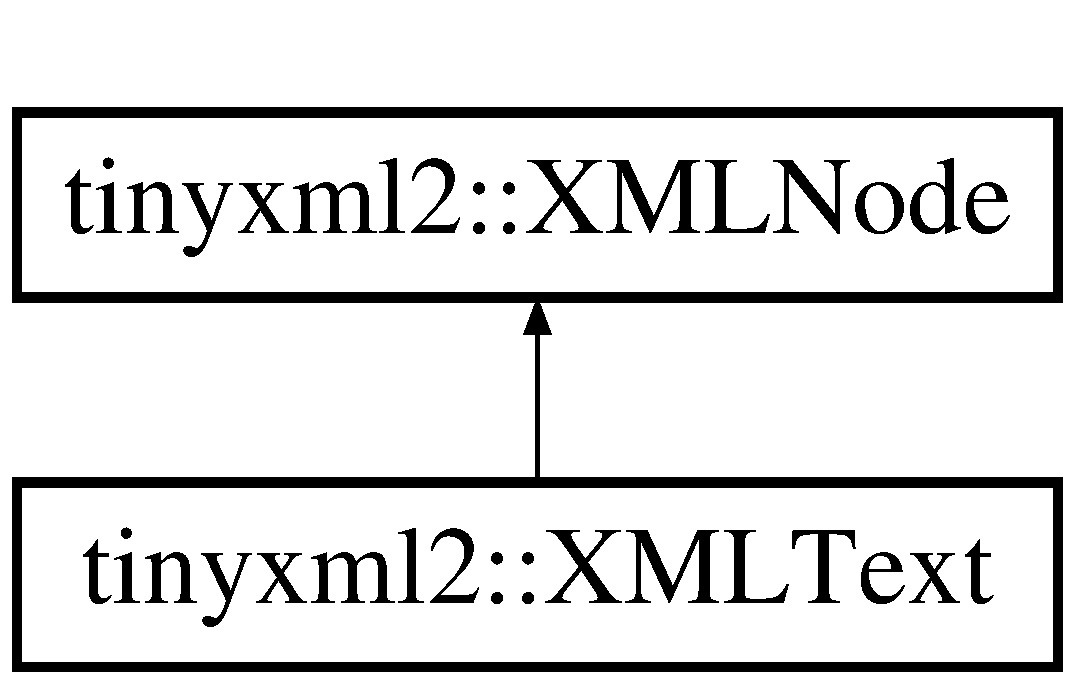
\includegraphics[height=2.000000cm]{classtinyxml2_1_1_x_m_l_text}
\end{center}
\end{figure}
\subsection*{Public Member Functions}
\begin{DoxyCompactItemize}
\item 
virtual bool \hyperlink{classtinyxml2_1_1_x_m_l_text_ae659d4fc7351a7df11c111cbe1ade46f}{Accept} (\hyperlink{classtinyxml2_1_1_x_m_l_visitor}{X\-M\-L\-Visitor} $\ast$visitor) const 
\item 
virtual \hyperlink{classtinyxml2_1_1_x_m_l_text}{X\-M\-L\-Text} $\ast$ \hyperlink{classtinyxml2_1_1_x_m_l_text_ab1213b4ddebe9b17ec7e7040e9f1caf7}{To\-Text} ()
\begin{DoxyCompactList}\small\item\em Safely cast to Text, or null. \end{DoxyCompactList}\item 
virtual const \hyperlink{classtinyxml2_1_1_x_m_l_text}{X\-M\-L\-Text} $\ast$ \hyperlink{classtinyxml2_1_1_x_m_l_text_a1e53cbc60968fe966790a65eaf87baaa}{To\-Text} () const 
\item 
void \hyperlink{classtinyxml2_1_1_x_m_l_text_ad080357d76ab7cc59d7651249949329d}{Set\-C\-Data} (bool is\-C\-Data)
\begin{DoxyCompactList}\small\item\em Declare whether this should be C\-D\-A\-T\-A or standard text. \end{DoxyCompactList}\item 
bool \hyperlink{classtinyxml2_1_1_x_m_l_text_a125574fe49da80efbae1349f20d02d41}{C\-Data} () const 
\begin{DoxyCompactList}\small\item\em Returns true if this is a C\-D\-A\-T\-A text element. \end{DoxyCompactList}\item 
char $\ast$ \hyperlink{classtinyxml2_1_1_x_m_l_text_ac18d9eec9f12b827b0d02b0847bf279e}{Parse\-Deep} (char $\ast$, \hyperlink{classtinyxml2_1_1_str_pair}{Str\-Pair} $\ast$end\-Tag)
\item 
virtual \hyperlink{classtinyxml2_1_1_x_m_l_node}{X\-M\-L\-Node} $\ast$ \hyperlink{classtinyxml2_1_1_x_m_l_text_af5115f8cc83de2947ed6a9d13e2f88c8}{Shallow\-Clone} (\hyperlink{classtinyxml2_1_1_x_m_l_document}{X\-M\-L\-Document} $\ast$document) const 
\item 
virtual bool \hyperlink{classtinyxml2_1_1_x_m_l_text_a1588aa5d23cb21eb31f36df0aaaa8d66}{Shallow\-Equal} (const \hyperlink{classtinyxml2_1_1_x_m_l_node}{X\-M\-L\-Node} $\ast$compare) const 
\end{DoxyCompactItemize}
\subsection*{Protected Member Functions}
\begin{DoxyCompactItemize}
\item 
\hyperlink{classtinyxml2_1_1_x_m_l_text_ad9f46d70e61e5386ead93728d8b90267}{X\-M\-L\-Text} (\hyperlink{classtinyxml2_1_1_x_m_l_document}{X\-M\-L\-Document} $\ast$doc)
\item 
virtual \hyperlink{classtinyxml2_1_1_x_m_l_text_ae9b8790d0dc13914394dbd7437c0e59d}{$\sim$\-X\-M\-L\-Text} ()
\item 
\hyperlink{classtinyxml2_1_1_x_m_l_text_a002156e1f61ee6d48e5368b7cca25582}{X\-M\-L\-Text} (const \hyperlink{classtinyxml2_1_1_x_m_l_text}{X\-M\-L\-Text} \&)
\item 
\hyperlink{classtinyxml2_1_1_x_m_l_text}{X\-M\-L\-Text} \& \hyperlink{classtinyxml2_1_1_x_m_l_text_ad8c9f398d92fa472e213b89d8483ae8f}{operator=} (const \hyperlink{classtinyxml2_1_1_x_m_l_text}{X\-M\-L\-Text} \&)
\end{DoxyCompactItemize}
\subsection*{Private Attributes}
\begin{DoxyCompactItemize}
\item 
bool \hyperlink{classtinyxml2_1_1_x_m_l_text_aae1a8b4117e8c8bb107900a0560d5ab5}{\-\_\-is\-C\-Data}
\end{DoxyCompactItemize}
\subsection*{Friends}
\begin{DoxyCompactItemize}
\item 
class \hyperlink{classtinyxml2_1_1_x_m_l_text_a449202cfc89e7ae5c2f81995476f9ec1}{X\-M\-L\-Base}
\item 
class \hyperlink{classtinyxml2_1_1_x_m_l_text_a4eee3bda60c60a30e4e8cd4ea91c4c6e}{X\-M\-L\-Document}
\end{DoxyCompactItemize}
\subsection*{Additional Inherited Members}


\subsection{Detailed Description}
X\-M\-L text.

Note that a text node can have child element nodes, for example\-: \begin{DoxyVerb}<root>This is <b>bold</b></root>
\end{DoxyVerb}


A text node can have 2 ways to output the next. \char`\"{}normal\char`\"{} output and C\-D\-A\-T\-A. It will default to the mode it was parsed from the X\-M\-L file and you generally want to leave it alone, but you can change the output mode with \hyperlink{classtinyxml2_1_1_x_m_l_text_ad080357d76ab7cc59d7651249949329d}{Set\-C\-Data()} and query it with \hyperlink{classtinyxml2_1_1_x_m_l_text_a125574fe49da80efbae1349f20d02d41}{C\-Data()}. 

\subsection{Constructor \& Destructor Documentation}
\hypertarget{classtinyxml2_1_1_x_m_l_text_ad9f46d70e61e5386ead93728d8b90267}{\index{tinyxml2\-::\-X\-M\-L\-Text@{tinyxml2\-::\-X\-M\-L\-Text}!X\-M\-L\-Text@{X\-M\-L\-Text}}
\index{X\-M\-L\-Text@{X\-M\-L\-Text}!tinyxml2::XMLText@{tinyxml2\-::\-X\-M\-L\-Text}}
\subsubsection[{X\-M\-L\-Text}]{\setlength{\rightskip}{0pt plus 5cm}tinyxml2\-::\-X\-M\-L\-Text\-::\-X\-M\-L\-Text (
\begin{DoxyParamCaption}
\item[{{\bf X\-M\-L\-Document} $\ast$}]{doc}
\end{DoxyParamCaption}
)\hspace{0.3cm}{\ttfamily [inline]}, {\ttfamily [protected]}}}\label{classtinyxml2_1_1_x_m_l_text_ad9f46d70e61e5386ead93728d8b90267}
\hypertarget{classtinyxml2_1_1_x_m_l_text_ae9b8790d0dc13914394dbd7437c0e59d}{\index{tinyxml2\-::\-X\-M\-L\-Text@{tinyxml2\-::\-X\-M\-L\-Text}!$\sim$\-X\-M\-L\-Text@{$\sim$\-X\-M\-L\-Text}}
\index{$\sim$\-X\-M\-L\-Text@{$\sim$\-X\-M\-L\-Text}!tinyxml2::XMLText@{tinyxml2\-::\-X\-M\-L\-Text}}
\subsubsection[{$\sim$\-X\-M\-L\-Text}]{\setlength{\rightskip}{0pt plus 5cm}virtual tinyxml2\-::\-X\-M\-L\-Text\-::$\sim$\-X\-M\-L\-Text (
\begin{DoxyParamCaption}
{}
\end{DoxyParamCaption}
)\hspace{0.3cm}{\ttfamily [inline]}, {\ttfamily [protected]}, {\ttfamily [virtual]}}}\label{classtinyxml2_1_1_x_m_l_text_ae9b8790d0dc13914394dbd7437c0e59d}
\hypertarget{classtinyxml2_1_1_x_m_l_text_a002156e1f61ee6d48e5368b7cca25582}{\index{tinyxml2\-::\-X\-M\-L\-Text@{tinyxml2\-::\-X\-M\-L\-Text}!X\-M\-L\-Text@{X\-M\-L\-Text}}
\index{X\-M\-L\-Text@{X\-M\-L\-Text}!tinyxml2::XMLText@{tinyxml2\-::\-X\-M\-L\-Text}}
\subsubsection[{X\-M\-L\-Text}]{\setlength{\rightskip}{0pt plus 5cm}tinyxml2\-::\-X\-M\-L\-Text\-::\-X\-M\-L\-Text (
\begin{DoxyParamCaption}
\item[{const {\bf X\-M\-L\-Text} \&}]{}
\end{DoxyParamCaption}
)\hspace{0.3cm}{\ttfamily [protected]}}}\label{classtinyxml2_1_1_x_m_l_text_a002156e1f61ee6d48e5368b7cca25582}


\subsection{Member Function Documentation}
\hypertarget{classtinyxml2_1_1_x_m_l_text_ae659d4fc7351a7df11c111cbe1ade46f}{\index{tinyxml2\-::\-X\-M\-L\-Text@{tinyxml2\-::\-X\-M\-L\-Text}!Accept@{Accept}}
\index{Accept@{Accept}!tinyxml2::XMLText@{tinyxml2\-::\-X\-M\-L\-Text}}
\subsubsection[{Accept}]{\setlength{\rightskip}{0pt plus 5cm}bool tinyxml2\-::\-X\-M\-L\-Text\-::\-Accept (
\begin{DoxyParamCaption}
\item[{{\bf X\-M\-L\-Visitor} $\ast$}]{visitor}
\end{DoxyParamCaption}
) const\hspace{0.3cm}{\ttfamily [virtual]}}}\label{classtinyxml2_1_1_x_m_l_text_ae659d4fc7351a7df11c111cbe1ade46f}
Accept a hierarchical visit of the nodes in the Tiny\-X\-M\-L-\/2 D\-O\-M. Every node in the X\-M\-L tree will be conditionally visited and the host will be called back via the \hyperlink{classtinyxml2_1_1_x_m_l_visitor}{X\-M\-L\-Visitor} interface.

This is essentially a S\-A\-X interface for Tiny\-X\-M\-L-\/2. (Note however it doesn't re-\/parse the X\-M\-L for the callbacks, so the performance of Tiny\-X\-M\-L-\/2 is unchanged by using this interface versus any other.)

The interface has been based on ideas from\-:
\begin{DoxyItemize}
\item \href{http://www.saxproject.org/}{\tt http\-://www.\-saxproject.\-org/}
\item \href{http://c2.com/cgi/wiki?HierarchicalVisitorPattern}{\tt http\-://c2.\-com/cgi/wiki?\-Hierarchical\-Visitor\-Pattern}
\end{DoxyItemize}

Which are both good references for \char`\"{}visiting\char`\"{}.

An example of using \hyperlink{classtinyxml2_1_1_x_m_l_text_ae659d4fc7351a7df11c111cbe1ade46f}{Accept()}\-: \begin{DoxyVerb}XMLPrinter printer;
tinyxmlDoc.Accept( &printer );
const char* xmlcstr = printer.CStr();
\end{DoxyVerb}
 

Implements \hyperlink{classtinyxml2_1_1_x_m_l_node_a81e66df0a44c67a7af17f3b77a152785}{tinyxml2\-::\-X\-M\-L\-Node}.

\hypertarget{classtinyxml2_1_1_x_m_l_text_a125574fe49da80efbae1349f20d02d41}{\index{tinyxml2\-::\-X\-M\-L\-Text@{tinyxml2\-::\-X\-M\-L\-Text}!C\-Data@{C\-Data}}
\index{C\-Data@{C\-Data}!tinyxml2::XMLText@{tinyxml2\-::\-X\-M\-L\-Text}}
\subsubsection[{C\-Data}]{\setlength{\rightskip}{0pt plus 5cm}bool tinyxml2\-::\-X\-M\-L\-Text\-::\-C\-Data (
\begin{DoxyParamCaption}
{}
\end{DoxyParamCaption}
) const\hspace{0.3cm}{\ttfamily [inline]}}}\label{classtinyxml2_1_1_x_m_l_text_a125574fe49da80efbae1349f20d02d41}


Returns true if this is a C\-D\-A\-T\-A text element. 

\hypertarget{classtinyxml2_1_1_x_m_l_text_ad8c9f398d92fa472e213b89d8483ae8f}{\index{tinyxml2\-::\-X\-M\-L\-Text@{tinyxml2\-::\-X\-M\-L\-Text}!operator=@{operator=}}
\index{operator=@{operator=}!tinyxml2::XMLText@{tinyxml2\-::\-X\-M\-L\-Text}}
\subsubsection[{operator=}]{\setlength{\rightskip}{0pt plus 5cm}{\bf X\-M\-L\-Text}\& tinyxml2\-::\-X\-M\-L\-Text\-::operator= (
\begin{DoxyParamCaption}
\item[{const {\bf X\-M\-L\-Text} \&}]{}
\end{DoxyParamCaption}
)\hspace{0.3cm}{\ttfamily [protected]}}}\label{classtinyxml2_1_1_x_m_l_text_ad8c9f398d92fa472e213b89d8483ae8f}
\hypertarget{classtinyxml2_1_1_x_m_l_text_ac18d9eec9f12b827b0d02b0847bf279e}{\index{tinyxml2\-::\-X\-M\-L\-Text@{tinyxml2\-::\-X\-M\-L\-Text}!Parse\-Deep@{Parse\-Deep}}
\index{Parse\-Deep@{Parse\-Deep}!tinyxml2::XMLText@{tinyxml2\-::\-X\-M\-L\-Text}}
\subsubsection[{Parse\-Deep}]{\setlength{\rightskip}{0pt plus 5cm}char $\ast$ tinyxml2\-::\-X\-M\-L\-Text\-::\-Parse\-Deep (
\begin{DoxyParamCaption}
\item[{char $\ast$}]{p, }
\item[{{\bf Str\-Pair} $\ast$}]{end\-Tag}
\end{DoxyParamCaption}
)\hspace{0.3cm}{\ttfamily [virtual]}}}\label{classtinyxml2_1_1_x_m_l_text_ac18d9eec9f12b827b0d02b0847bf279e}


Reimplemented from \hyperlink{classtinyxml2_1_1_x_m_l_node_a7610d0f603e8b603d2078521811a23c1}{tinyxml2\-::\-X\-M\-L\-Node}.

\hypertarget{classtinyxml2_1_1_x_m_l_text_ad080357d76ab7cc59d7651249949329d}{\index{tinyxml2\-::\-X\-M\-L\-Text@{tinyxml2\-::\-X\-M\-L\-Text}!Set\-C\-Data@{Set\-C\-Data}}
\index{Set\-C\-Data@{Set\-C\-Data}!tinyxml2::XMLText@{tinyxml2\-::\-X\-M\-L\-Text}}
\subsubsection[{Set\-C\-Data}]{\setlength{\rightskip}{0pt plus 5cm}void tinyxml2\-::\-X\-M\-L\-Text\-::\-Set\-C\-Data (
\begin{DoxyParamCaption}
\item[{bool}]{is\-C\-Data}
\end{DoxyParamCaption}
)\hspace{0.3cm}{\ttfamily [inline]}}}\label{classtinyxml2_1_1_x_m_l_text_ad080357d76ab7cc59d7651249949329d}


Declare whether this should be C\-D\-A\-T\-A or standard text. 

\hypertarget{classtinyxml2_1_1_x_m_l_text_af5115f8cc83de2947ed6a9d13e2f88c8}{\index{tinyxml2\-::\-X\-M\-L\-Text@{tinyxml2\-::\-X\-M\-L\-Text}!Shallow\-Clone@{Shallow\-Clone}}
\index{Shallow\-Clone@{Shallow\-Clone}!tinyxml2::XMLText@{tinyxml2\-::\-X\-M\-L\-Text}}
\subsubsection[{Shallow\-Clone}]{\setlength{\rightskip}{0pt plus 5cm}{\bf X\-M\-L\-Node} $\ast$ tinyxml2\-::\-X\-M\-L\-Text\-::\-Shallow\-Clone (
\begin{DoxyParamCaption}
\item[{{\bf X\-M\-L\-Document} $\ast$}]{document}
\end{DoxyParamCaption}
) const\hspace{0.3cm}{\ttfamily [virtual]}}}\label{classtinyxml2_1_1_x_m_l_text_af5115f8cc83de2947ed6a9d13e2f88c8}
Make a copy of this node, but not its children. You may pass in a Document pointer that will be the owner of the new Node. If the 'document' is null, then the node returned will be allocated from the current Document. (this-\/$>$\hyperlink{classtinyxml2_1_1_x_m_l_node_af343d1ef0b45c0020e62d784d7e67a68}{Get\-Document()})

Note\-: if called on a \hyperlink{classtinyxml2_1_1_x_m_l_document}{X\-M\-L\-Document}, this will return null. 

Implements \hyperlink{classtinyxml2_1_1_x_m_l_node_a8402cbd3129d20e9e6024bbcc0531283}{tinyxml2\-::\-X\-M\-L\-Node}.

\hypertarget{classtinyxml2_1_1_x_m_l_text_a1588aa5d23cb21eb31f36df0aaaa8d66}{\index{tinyxml2\-::\-X\-M\-L\-Text@{tinyxml2\-::\-X\-M\-L\-Text}!Shallow\-Equal@{Shallow\-Equal}}
\index{Shallow\-Equal@{Shallow\-Equal}!tinyxml2::XMLText@{tinyxml2\-::\-X\-M\-L\-Text}}
\subsubsection[{Shallow\-Equal}]{\setlength{\rightskip}{0pt plus 5cm}bool tinyxml2\-::\-X\-M\-L\-Text\-::\-Shallow\-Equal (
\begin{DoxyParamCaption}
\item[{const {\bf X\-M\-L\-Node} $\ast$}]{compare}
\end{DoxyParamCaption}
) const\hspace{0.3cm}{\ttfamily [virtual]}}}\label{classtinyxml2_1_1_x_m_l_text_a1588aa5d23cb21eb31f36df0aaaa8d66}
Test if 2 nodes are the same, but don't test children. The 2 nodes do not need to be in the same Document.

Note\-: if called on a \hyperlink{classtinyxml2_1_1_x_m_l_document}{X\-M\-L\-Document}, this will return false. 

Implements \hyperlink{classtinyxml2_1_1_x_m_l_node_a7ce18b751c3ea09eac292dca264f9226}{tinyxml2\-::\-X\-M\-L\-Node}.

\hypertarget{classtinyxml2_1_1_x_m_l_text_ab1213b4ddebe9b17ec7e7040e9f1caf7}{\index{tinyxml2\-::\-X\-M\-L\-Text@{tinyxml2\-::\-X\-M\-L\-Text}!To\-Text@{To\-Text}}
\index{To\-Text@{To\-Text}!tinyxml2::XMLText@{tinyxml2\-::\-X\-M\-L\-Text}}
\subsubsection[{To\-Text}]{\setlength{\rightskip}{0pt plus 5cm}virtual {\bf X\-M\-L\-Text}$\ast$ tinyxml2\-::\-X\-M\-L\-Text\-::\-To\-Text (
\begin{DoxyParamCaption}
{}
\end{DoxyParamCaption}
)\hspace{0.3cm}{\ttfamily [inline]}, {\ttfamily [virtual]}}}\label{classtinyxml2_1_1_x_m_l_text_ab1213b4ddebe9b17ec7e7040e9f1caf7}


Safely cast to Text, or null. 



Reimplemented from \hyperlink{classtinyxml2_1_1_x_m_l_node_a41c55dab9162d1eb62db2008430e376b}{tinyxml2\-::\-X\-M\-L\-Node}.

\hypertarget{classtinyxml2_1_1_x_m_l_text_a1e53cbc60968fe966790a65eaf87baaa}{\index{tinyxml2\-::\-X\-M\-L\-Text@{tinyxml2\-::\-X\-M\-L\-Text}!To\-Text@{To\-Text}}
\index{To\-Text@{To\-Text}!tinyxml2::XMLText@{tinyxml2\-::\-X\-M\-L\-Text}}
\subsubsection[{To\-Text}]{\setlength{\rightskip}{0pt plus 5cm}virtual const {\bf X\-M\-L\-Text}$\ast$ tinyxml2\-::\-X\-M\-L\-Text\-::\-To\-Text (
\begin{DoxyParamCaption}
{}
\end{DoxyParamCaption}
) const\hspace{0.3cm}{\ttfamily [inline]}, {\ttfamily [virtual]}}}\label{classtinyxml2_1_1_x_m_l_text_a1e53cbc60968fe966790a65eaf87baaa}


Reimplemented from \hyperlink{classtinyxml2_1_1_x_m_l_node_a89009ffc1b9f5d692bf8d4c9f18c3bec}{tinyxml2\-::\-X\-M\-L\-Node}.



\subsection{Friends And Related Function Documentation}
\hypertarget{classtinyxml2_1_1_x_m_l_text_a449202cfc89e7ae5c2f81995476f9ec1}{\index{tinyxml2\-::\-X\-M\-L\-Text@{tinyxml2\-::\-X\-M\-L\-Text}!X\-M\-L\-Base@{X\-M\-L\-Base}}
\index{X\-M\-L\-Base@{X\-M\-L\-Base}!tinyxml2::XMLText@{tinyxml2\-::\-X\-M\-L\-Text}}
\subsubsection[{X\-M\-L\-Base}]{\setlength{\rightskip}{0pt plus 5cm}friend class X\-M\-L\-Base\hspace{0.3cm}{\ttfamily [friend]}}}\label{classtinyxml2_1_1_x_m_l_text_a449202cfc89e7ae5c2f81995476f9ec1}
\hypertarget{classtinyxml2_1_1_x_m_l_text_a4eee3bda60c60a30e4e8cd4ea91c4c6e}{\index{tinyxml2\-::\-X\-M\-L\-Text@{tinyxml2\-::\-X\-M\-L\-Text}!X\-M\-L\-Document@{X\-M\-L\-Document}}
\index{X\-M\-L\-Document@{X\-M\-L\-Document}!tinyxml2::XMLText@{tinyxml2\-::\-X\-M\-L\-Text}}
\subsubsection[{X\-M\-L\-Document}]{\setlength{\rightskip}{0pt plus 5cm}friend class {\bf X\-M\-L\-Document}\hspace{0.3cm}{\ttfamily [friend]}}}\label{classtinyxml2_1_1_x_m_l_text_a4eee3bda60c60a30e4e8cd4ea91c4c6e}


\subsection{Member Data Documentation}
\hypertarget{classtinyxml2_1_1_x_m_l_text_aae1a8b4117e8c8bb107900a0560d5ab5}{\index{tinyxml2\-::\-X\-M\-L\-Text@{tinyxml2\-::\-X\-M\-L\-Text}!\-\_\-is\-C\-Data@{\-\_\-is\-C\-Data}}
\index{\-\_\-is\-C\-Data@{\-\_\-is\-C\-Data}!tinyxml2::XMLText@{tinyxml2\-::\-X\-M\-L\-Text}}
\subsubsection[{\-\_\-is\-C\-Data}]{\setlength{\rightskip}{0pt plus 5cm}bool tinyxml2\-::\-X\-M\-L\-Text\-::\-\_\-is\-C\-Data\hspace{0.3cm}{\ttfamily [private]}}}\label{classtinyxml2_1_1_x_m_l_text_aae1a8b4117e8c8bb107900a0560d5ab5}


The documentation for this class was generated from the following files\-:\begin{DoxyCompactItemize}
\item 
Utils/\-X\-M\-L\-\_\-\-Config/\hyperlink{tinyxml2_8h}{tinyxml2.\-h}\item 
Utils/\-X\-M\-L\-\_\-\-Config/\hyperlink{tinyxml2_8cpp}{tinyxml2.\-cpp}\end{DoxyCompactItemize}

\hypertarget{classtinyxml2_1_1_x_m_l_unknown}{\section{tinyxml2\-:\-:X\-M\-L\-Unknown Class Reference}
\label{classtinyxml2_1_1_x_m_l_unknown}\index{tinyxml2\-::\-X\-M\-L\-Unknown@{tinyxml2\-::\-X\-M\-L\-Unknown}}
}


{\ttfamily \#include $<$tinyxml2.\-h$>$}

Inheritance diagram for tinyxml2\-:\-:X\-M\-L\-Unknown\-:\begin{figure}[H]
\begin{center}
\leavevmode
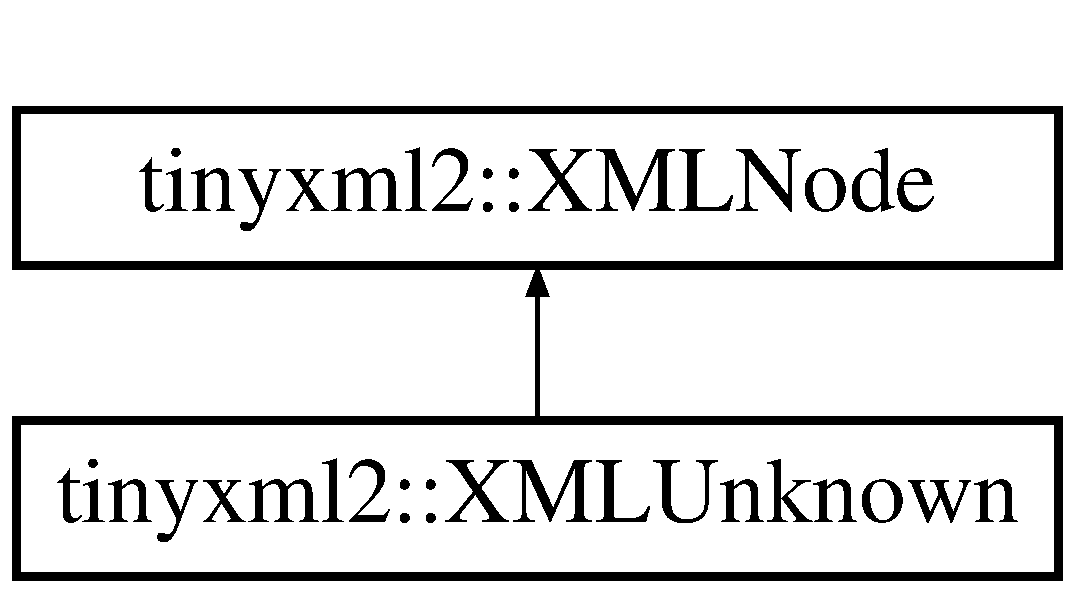
\includegraphics[height=2.000000cm]{classtinyxml2_1_1_x_m_l_unknown}
\end{center}
\end{figure}
\subsection*{Public Member Functions}
\begin{DoxyCompactItemize}
\item 
virtual \hyperlink{classtinyxml2_1_1_x_m_l_unknown}{X\-M\-L\-Unknown} $\ast$ \hyperlink{classtinyxml2_1_1_x_m_l_unknown_af4374856421921cad578c8affae872b6}{To\-Unknown} ()
\begin{DoxyCompactList}\small\item\em Safely cast to an Unknown, or null. \end{DoxyCompactList}\item 
virtual const \hyperlink{classtinyxml2_1_1_x_m_l_unknown}{X\-M\-L\-Unknown} $\ast$ \hyperlink{classtinyxml2_1_1_x_m_l_unknown_a257987e79955399e6e9f119b58d4bb30}{To\-Unknown} () const 
\item 
virtual bool \hyperlink{classtinyxml2_1_1_x_m_l_unknown_a0d341ab804a1438a474810bb5bd29dd5}{Accept} (\hyperlink{classtinyxml2_1_1_x_m_l_visitor}{X\-M\-L\-Visitor} $\ast$visitor) const 
\item 
char $\ast$ \hyperlink{classtinyxml2_1_1_x_m_l_unknown_a0e4f3509dee42a4d45a7f0002be568cc}{Parse\-Deep} (char $\ast$, \hyperlink{classtinyxml2_1_1_str_pair}{Str\-Pair} $\ast$end\-Tag)
\item 
virtual \hyperlink{classtinyxml2_1_1_x_m_l_node}{X\-M\-L\-Node} $\ast$ \hyperlink{classtinyxml2_1_1_x_m_l_unknown_aa09fc7cb0cd64d6bb9c5ae00ffc549ec}{Shallow\-Clone} (\hyperlink{classtinyxml2_1_1_x_m_l_document}{X\-M\-L\-Document} $\ast$document) const 
\item 
virtual bool \hyperlink{classtinyxml2_1_1_x_m_l_unknown_a0169df157bf69a092b404ca49621ff1a}{Shallow\-Equal} (const \hyperlink{classtinyxml2_1_1_x_m_l_node}{X\-M\-L\-Node} $\ast$compare) const 
\end{DoxyCompactItemize}
\subsection*{Protected Member Functions}
\begin{DoxyCompactItemize}
\item 
\hyperlink{classtinyxml2_1_1_x_m_l_unknown_a9391eb679598d50baba424e6f1aa367b}{X\-M\-L\-Unknown} (\hyperlink{classtinyxml2_1_1_x_m_l_document}{X\-M\-L\-Document} $\ast$doc)
\item 
virtual \hyperlink{classtinyxml2_1_1_x_m_l_unknown_a86fcd722ca173a7f385bafafa879f26e}{$\sim$\-X\-M\-L\-Unknown} ()
\item 
\hyperlink{classtinyxml2_1_1_x_m_l_unknown_aab31a93c95a7cedc9597cea7caffa73f}{X\-M\-L\-Unknown} (const \hyperlink{classtinyxml2_1_1_x_m_l_unknown}{X\-M\-L\-Unknown} \&)
\item 
\hyperlink{classtinyxml2_1_1_x_m_l_unknown}{X\-M\-L\-Unknown} \& \hyperlink{classtinyxml2_1_1_x_m_l_unknown_a6137d5611db42c35de3d869f66555e5b}{operator=} (const \hyperlink{classtinyxml2_1_1_x_m_l_unknown}{X\-M\-L\-Unknown} \&)
\end{DoxyCompactItemize}
\subsection*{Friends}
\begin{DoxyCompactItemize}
\item 
class \hyperlink{classtinyxml2_1_1_x_m_l_unknown_a4eee3bda60c60a30e4e8cd4ea91c4c6e}{X\-M\-L\-Document}
\end{DoxyCompactItemize}
\subsection*{Additional Inherited Members}


\subsection{Detailed Description}
Any tag that Tiny\-X\-M\-L-\/2 doesn't recognize is saved as an unknown. It is a tag of text, but should not be modified. It will be written back to the X\-M\-L, unchanged, when the file is saved.

D\-T\-D tags get thrown into X\-M\-L\-Unknowns. 

\subsection{Constructor \& Destructor Documentation}
\hypertarget{classtinyxml2_1_1_x_m_l_unknown_a9391eb679598d50baba424e6f1aa367b}{\index{tinyxml2\-::\-X\-M\-L\-Unknown@{tinyxml2\-::\-X\-M\-L\-Unknown}!X\-M\-L\-Unknown@{X\-M\-L\-Unknown}}
\index{X\-M\-L\-Unknown@{X\-M\-L\-Unknown}!tinyxml2::XMLUnknown@{tinyxml2\-::\-X\-M\-L\-Unknown}}
\subsubsection[{X\-M\-L\-Unknown}]{\setlength{\rightskip}{0pt plus 5cm}tinyxml2\-::\-X\-M\-L\-Unknown\-::\-X\-M\-L\-Unknown (
\begin{DoxyParamCaption}
\item[{{\bf X\-M\-L\-Document} $\ast$}]{doc}
\end{DoxyParamCaption}
)\hspace{0.3cm}{\ttfamily [protected]}}}\label{classtinyxml2_1_1_x_m_l_unknown_a9391eb679598d50baba424e6f1aa367b}
\hypertarget{classtinyxml2_1_1_x_m_l_unknown_a86fcd722ca173a7f385bafafa879f26e}{\index{tinyxml2\-::\-X\-M\-L\-Unknown@{tinyxml2\-::\-X\-M\-L\-Unknown}!$\sim$\-X\-M\-L\-Unknown@{$\sim$\-X\-M\-L\-Unknown}}
\index{$\sim$\-X\-M\-L\-Unknown@{$\sim$\-X\-M\-L\-Unknown}!tinyxml2::XMLUnknown@{tinyxml2\-::\-X\-M\-L\-Unknown}}
\subsubsection[{$\sim$\-X\-M\-L\-Unknown}]{\setlength{\rightskip}{0pt plus 5cm}tinyxml2\-::\-X\-M\-L\-Unknown\-::$\sim$\-X\-M\-L\-Unknown (
\begin{DoxyParamCaption}
{}
\end{DoxyParamCaption}
)\hspace{0.3cm}{\ttfamily [protected]}, {\ttfamily [virtual]}}}\label{classtinyxml2_1_1_x_m_l_unknown_a86fcd722ca173a7f385bafafa879f26e}
\hypertarget{classtinyxml2_1_1_x_m_l_unknown_aab31a93c95a7cedc9597cea7caffa73f}{\index{tinyxml2\-::\-X\-M\-L\-Unknown@{tinyxml2\-::\-X\-M\-L\-Unknown}!X\-M\-L\-Unknown@{X\-M\-L\-Unknown}}
\index{X\-M\-L\-Unknown@{X\-M\-L\-Unknown}!tinyxml2::XMLUnknown@{tinyxml2\-::\-X\-M\-L\-Unknown}}
\subsubsection[{X\-M\-L\-Unknown}]{\setlength{\rightskip}{0pt plus 5cm}tinyxml2\-::\-X\-M\-L\-Unknown\-::\-X\-M\-L\-Unknown (
\begin{DoxyParamCaption}
\item[{const {\bf X\-M\-L\-Unknown} \&}]{}
\end{DoxyParamCaption}
)\hspace{0.3cm}{\ttfamily [protected]}}}\label{classtinyxml2_1_1_x_m_l_unknown_aab31a93c95a7cedc9597cea7caffa73f}


\subsection{Member Function Documentation}
\hypertarget{classtinyxml2_1_1_x_m_l_unknown_a0d341ab804a1438a474810bb5bd29dd5}{\index{tinyxml2\-::\-X\-M\-L\-Unknown@{tinyxml2\-::\-X\-M\-L\-Unknown}!Accept@{Accept}}
\index{Accept@{Accept}!tinyxml2::XMLUnknown@{tinyxml2\-::\-X\-M\-L\-Unknown}}
\subsubsection[{Accept}]{\setlength{\rightskip}{0pt plus 5cm}bool tinyxml2\-::\-X\-M\-L\-Unknown\-::\-Accept (
\begin{DoxyParamCaption}
\item[{{\bf X\-M\-L\-Visitor} $\ast$}]{visitor}
\end{DoxyParamCaption}
) const\hspace{0.3cm}{\ttfamily [virtual]}}}\label{classtinyxml2_1_1_x_m_l_unknown_a0d341ab804a1438a474810bb5bd29dd5}
Accept a hierarchical visit of the nodes in the Tiny\-X\-M\-L-\/2 D\-O\-M. Every node in the X\-M\-L tree will be conditionally visited and the host will be called back via the \hyperlink{classtinyxml2_1_1_x_m_l_visitor}{X\-M\-L\-Visitor} interface.

This is essentially a S\-A\-X interface for Tiny\-X\-M\-L-\/2. (Note however it doesn't re-\/parse the X\-M\-L for the callbacks, so the performance of Tiny\-X\-M\-L-\/2 is unchanged by using this interface versus any other.)

The interface has been based on ideas from\-:
\begin{DoxyItemize}
\item \href{http://www.saxproject.org/}{\tt http\-://www.\-saxproject.\-org/}
\item \href{http://c2.com/cgi/wiki?HierarchicalVisitorPattern}{\tt http\-://c2.\-com/cgi/wiki?\-Hierarchical\-Visitor\-Pattern}
\end{DoxyItemize}

Which are both good references for \char`\"{}visiting\char`\"{}.

An example of using \hyperlink{classtinyxml2_1_1_x_m_l_unknown_a0d341ab804a1438a474810bb5bd29dd5}{Accept()}\-: \begin{DoxyVerb}XMLPrinter printer;
tinyxmlDoc.Accept( &printer );
const char* xmlcstr = printer.CStr();
\end{DoxyVerb}
 

Implements \hyperlink{classtinyxml2_1_1_x_m_l_node_a81e66df0a44c67a7af17f3b77a152785}{tinyxml2\-::\-X\-M\-L\-Node}.

\hypertarget{classtinyxml2_1_1_x_m_l_unknown_a6137d5611db42c35de3d869f66555e5b}{\index{tinyxml2\-::\-X\-M\-L\-Unknown@{tinyxml2\-::\-X\-M\-L\-Unknown}!operator=@{operator=}}
\index{operator=@{operator=}!tinyxml2::XMLUnknown@{tinyxml2\-::\-X\-M\-L\-Unknown}}
\subsubsection[{operator=}]{\setlength{\rightskip}{0pt plus 5cm}{\bf X\-M\-L\-Unknown}\& tinyxml2\-::\-X\-M\-L\-Unknown\-::operator= (
\begin{DoxyParamCaption}
\item[{const {\bf X\-M\-L\-Unknown} \&}]{}
\end{DoxyParamCaption}
)\hspace{0.3cm}{\ttfamily [protected]}}}\label{classtinyxml2_1_1_x_m_l_unknown_a6137d5611db42c35de3d869f66555e5b}
\hypertarget{classtinyxml2_1_1_x_m_l_unknown_a0e4f3509dee42a4d45a7f0002be568cc}{\index{tinyxml2\-::\-X\-M\-L\-Unknown@{tinyxml2\-::\-X\-M\-L\-Unknown}!Parse\-Deep@{Parse\-Deep}}
\index{Parse\-Deep@{Parse\-Deep}!tinyxml2::XMLUnknown@{tinyxml2\-::\-X\-M\-L\-Unknown}}
\subsubsection[{Parse\-Deep}]{\setlength{\rightskip}{0pt plus 5cm}char $\ast$ tinyxml2\-::\-X\-M\-L\-Unknown\-::\-Parse\-Deep (
\begin{DoxyParamCaption}
\item[{char $\ast$}]{p, }
\item[{{\bf Str\-Pair} $\ast$}]{end\-Tag}
\end{DoxyParamCaption}
)\hspace{0.3cm}{\ttfamily [virtual]}}}\label{classtinyxml2_1_1_x_m_l_unknown_a0e4f3509dee42a4d45a7f0002be568cc}


Reimplemented from \hyperlink{classtinyxml2_1_1_x_m_l_node_a7610d0f603e8b603d2078521811a23c1}{tinyxml2\-::\-X\-M\-L\-Node}.

\hypertarget{classtinyxml2_1_1_x_m_l_unknown_aa09fc7cb0cd64d6bb9c5ae00ffc549ec}{\index{tinyxml2\-::\-X\-M\-L\-Unknown@{tinyxml2\-::\-X\-M\-L\-Unknown}!Shallow\-Clone@{Shallow\-Clone}}
\index{Shallow\-Clone@{Shallow\-Clone}!tinyxml2::XMLUnknown@{tinyxml2\-::\-X\-M\-L\-Unknown}}
\subsubsection[{Shallow\-Clone}]{\setlength{\rightskip}{0pt plus 5cm}{\bf X\-M\-L\-Node} $\ast$ tinyxml2\-::\-X\-M\-L\-Unknown\-::\-Shallow\-Clone (
\begin{DoxyParamCaption}
\item[{{\bf X\-M\-L\-Document} $\ast$}]{document}
\end{DoxyParamCaption}
) const\hspace{0.3cm}{\ttfamily [virtual]}}}\label{classtinyxml2_1_1_x_m_l_unknown_aa09fc7cb0cd64d6bb9c5ae00ffc549ec}
Make a copy of this node, but not its children. You may pass in a Document pointer that will be the owner of the new Node. If the 'document' is null, then the node returned will be allocated from the current Document. (this-\/$>$\hyperlink{classtinyxml2_1_1_x_m_l_node_af343d1ef0b45c0020e62d784d7e67a68}{Get\-Document()})

Note\-: if called on a \hyperlink{classtinyxml2_1_1_x_m_l_document}{X\-M\-L\-Document}, this will return null. 

Implements \hyperlink{classtinyxml2_1_1_x_m_l_node_a8402cbd3129d20e9e6024bbcc0531283}{tinyxml2\-::\-X\-M\-L\-Node}.

\hypertarget{classtinyxml2_1_1_x_m_l_unknown_a0169df157bf69a092b404ca49621ff1a}{\index{tinyxml2\-::\-X\-M\-L\-Unknown@{tinyxml2\-::\-X\-M\-L\-Unknown}!Shallow\-Equal@{Shallow\-Equal}}
\index{Shallow\-Equal@{Shallow\-Equal}!tinyxml2::XMLUnknown@{tinyxml2\-::\-X\-M\-L\-Unknown}}
\subsubsection[{Shallow\-Equal}]{\setlength{\rightskip}{0pt plus 5cm}bool tinyxml2\-::\-X\-M\-L\-Unknown\-::\-Shallow\-Equal (
\begin{DoxyParamCaption}
\item[{const {\bf X\-M\-L\-Node} $\ast$}]{compare}
\end{DoxyParamCaption}
) const\hspace{0.3cm}{\ttfamily [virtual]}}}\label{classtinyxml2_1_1_x_m_l_unknown_a0169df157bf69a092b404ca49621ff1a}
Test if 2 nodes are the same, but don't test children. The 2 nodes do not need to be in the same Document.

Note\-: if called on a \hyperlink{classtinyxml2_1_1_x_m_l_document}{X\-M\-L\-Document}, this will return false. 

Implements \hyperlink{classtinyxml2_1_1_x_m_l_node_a7ce18b751c3ea09eac292dca264f9226}{tinyxml2\-::\-X\-M\-L\-Node}.

\hypertarget{classtinyxml2_1_1_x_m_l_unknown_af4374856421921cad578c8affae872b6}{\index{tinyxml2\-::\-X\-M\-L\-Unknown@{tinyxml2\-::\-X\-M\-L\-Unknown}!To\-Unknown@{To\-Unknown}}
\index{To\-Unknown@{To\-Unknown}!tinyxml2::XMLUnknown@{tinyxml2\-::\-X\-M\-L\-Unknown}}
\subsubsection[{To\-Unknown}]{\setlength{\rightskip}{0pt plus 5cm}virtual {\bf X\-M\-L\-Unknown}$\ast$ tinyxml2\-::\-X\-M\-L\-Unknown\-::\-To\-Unknown (
\begin{DoxyParamCaption}
{}
\end{DoxyParamCaption}
)\hspace{0.3cm}{\ttfamily [inline]}, {\ttfamily [virtual]}}}\label{classtinyxml2_1_1_x_m_l_unknown_af4374856421921cad578c8affae872b6}


Safely cast to an Unknown, or null. 



Reimplemented from \hyperlink{classtinyxml2_1_1_x_m_l_node_a8675a74aa0ada6eccab0c77ef3e5b9bd}{tinyxml2\-::\-X\-M\-L\-Node}.

\hypertarget{classtinyxml2_1_1_x_m_l_unknown_a257987e79955399e6e9f119b58d4bb30}{\index{tinyxml2\-::\-X\-M\-L\-Unknown@{tinyxml2\-::\-X\-M\-L\-Unknown}!To\-Unknown@{To\-Unknown}}
\index{To\-Unknown@{To\-Unknown}!tinyxml2::XMLUnknown@{tinyxml2\-::\-X\-M\-L\-Unknown}}
\subsubsection[{To\-Unknown}]{\setlength{\rightskip}{0pt plus 5cm}virtual const {\bf X\-M\-L\-Unknown}$\ast$ tinyxml2\-::\-X\-M\-L\-Unknown\-::\-To\-Unknown (
\begin{DoxyParamCaption}
{}
\end{DoxyParamCaption}
) const\hspace{0.3cm}{\ttfamily [inline]}, {\ttfamily [virtual]}}}\label{classtinyxml2_1_1_x_m_l_unknown_a257987e79955399e6e9f119b58d4bb30}


Reimplemented from \hyperlink{classtinyxml2_1_1_x_m_l_node_a71f5ae90296dbe67979f83fe97073efa}{tinyxml2\-::\-X\-M\-L\-Node}.



\subsection{Friends And Related Function Documentation}
\hypertarget{classtinyxml2_1_1_x_m_l_unknown_a4eee3bda60c60a30e4e8cd4ea91c4c6e}{\index{tinyxml2\-::\-X\-M\-L\-Unknown@{tinyxml2\-::\-X\-M\-L\-Unknown}!X\-M\-L\-Document@{X\-M\-L\-Document}}
\index{X\-M\-L\-Document@{X\-M\-L\-Document}!tinyxml2::XMLUnknown@{tinyxml2\-::\-X\-M\-L\-Unknown}}
\subsubsection[{X\-M\-L\-Document}]{\setlength{\rightskip}{0pt plus 5cm}friend class {\bf X\-M\-L\-Document}\hspace{0.3cm}{\ttfamily [friend]}}}\label{classtinyxml2_1_1_x_m_l_unknown_a4eee3bda60c60a30e4e8cd4ea91c4c6e}


The documentation for this class was generated from the following files\-:\begin{DoxyCompactItemize}
\item 
Utils/\-X\-M\-L\-\_\-\-Config/\hyperlink{tinyxml2_8h}{tinyxml2.\-h}\item 
Utils/\-X\-M\-L\-\_\-\-Config/\hyperlink{tinyxml2_8cpp}{tinyxml2.\-cpp}\end{DoxyCompactItemize}

\hypertarget{classtinyxml2_1_1_x_m_l_util}{\section{tinyxml2\-:\-:X\-M\-L\-Util Class Reference}
\label{classtinyxml2_1_1_x_m_l_util}\index{tinyxml2\-::\-X\-M\-L\-Util@{tinyxml2\-::\-X\-M\-L\-Util}}
}


{\ttfamily \#include $<$tinyxml2.\-h$>$}

\subsection*{Static Public Member Functions}
\begin{DoxyCompactItemize}
\item 
static const char $\ast$ \hyperlink{classtinyxml2_1_1_x_m_l_util_a9333d20f2a34325b5115ca45849c4b2a}{Skip\-White\-Space} (const char $\ast$p)
\item 
static char $\ast$ \hyperlink{classtinyxml2_1_1_x_m_l_util_aa48025be8843ec5a79b65579d31bd8fc}{Skip\-White\-Space} (char $\ast$p)
\item 
static bool \hyperlink{classtinyxml2_1_1_x_m_l_util_a357ec3af8fc433d19023a815f45e8e33}{Is\-White\-Space} (char p)
\item 
static bool \hyperlink{classtinyxml2_1_1_x_m_l_util_abe106a69ac4d942a4381a4d9dfd0e0bd}{Is\-Name\-Start\-Char} (unsigned char ch)
\item 
static bool \hyperlink{classtinyxml2_1_1_x_m_l_util_a04b17341538fa11752f24b4301d19485}{Is\-Name\-Char} (unsigned char ch)
\item 
static bool \hyperlink{classtinyxml2_1_1_x_m_l_util_acfcd287cacfd2533e1bc9ea4dfb56602}{String\-Equal} (const char $\ast$p, const char $\ast$q, int n\-Char=I\-N\-T\-\_\-\-M\-A\-X)
\item 
static int \hyperlink{classtinyxml2_1_1_x_m_l_util_a24ba87b1d22528167a3d16c4f52096bf}{Is\-U\-T\-F8\-Continuation} (const char p)
\item 
static const char $\ast$ \hyperlink{classtinyxml2_1_1_x_m_l_util_ae9bcb2bc3cd6475fdc644c8c17790555}{Read\-B\-O\-M} (const char $\ast$p, bool $\ast$has\-B\-O\-M)
\item 
static const char $\ast$ \hyperlink{classtinyxml2_1_1_x_m_l_util_a5a96e5144a8d693dc4bcd783d9964648}{Get\-Character\-Ref} (const char $\ast$p, char $\ast$value, int $\ast$length)
\item 
static void \hyperlink{classtinyxml2_1_1_x_m_l_util_a31c00d5c5dfb38382de1dfcaf4be3595}{Convert\-U\-T\-F32\-To\-U\-T\-F8} (unsigned long input, char $\ast$output, int $\ast$length)
\item 
static void \hyperlink{classtinyxml2_1_1_x_m_l_util_a3cd6c703d49b9d51bdf0f4ff6aa021c7}{To\-Str} (int v, char $\ast$buffer, int buffer\-Size)
\item 
static void \hyperlink{classtinyxml2_1_1_x_m_l_util_ac00c2e52c1c36dab3ff41d86a9bf60f9}{To\-Str} (unsigned v, char $\ast$buffer, int buffer\-Size)
\item 
static void \hyperlink{classtinyxml2_1_1_x_m_l_util_adba0718527ae9e80f663a71ea325cb11}{To\-Str} (bool v, char $\ast$buffer, int buffer\-Size)
\item 
static void \hyperlink{classtinyxml2_1_1_x_m_l_util_a8957ad44fee5fa02ba52d73aad4d0a31}{To\-Str} (float v, char $\ast$buffer, int buffer\-Size)
\item 
static void \hyperlink{classtinyxml2_1_1_x_m_l_util_a1cd141e50980fcddd6bf9af5de4b1db7}{To\-Str} (double v, char $\ast$buffer, int buffer\-Size)
\item 
static bool \hyperlink{classtinyxml2_1_1_x_m_l_util_ad4df4023d11ee3fca9689c49b9707323}{To\-Int} (const char $\ast$str, int $\ast$value)
\item 
static bool \hyperlink{classtinyxml2_1_1_x_m_l_util_a210c8637d5eb4ce3d4625294af0efc2f}{To\-Unsigned} (const char $\ast$str, unsigned $\ast$value)
\item 
static bool \hyperlink{classtinyxml2_1_1_x_m_l_util_ae5b03e0a1ca5d42052a7ac540f7aa12a}{To\-Bool} (const char $\ast$str, bool $\ast$value)
\item 
static bool \hyperlink{classtinyxml2_1_1_x_m_l_util_a399e71edb5f29d61ea81d91ee0332bb9}{To\-Float} (const char $\ast$str, float $\ast$value)
\item 
static bool \hyperlink{classtinyxml2_1_1_x_m_l_util_ad8f75ac140fb19c1c6e164a957c4cd53}{To\-Double} (const char $\ast$str, double $\ast$value)
\end{DoxyCompactItemize}


\subsection{Member Function Documentation}
\hypertarget{classtinyxml2_1_1_x_m_l_util_a31c00d5c5dfb38382de1dfcaf4be3595}{\index{tinyxml2\-::\-X\-M\-L\-Util@{tinyxml2\-::\-X\-M\-L\-Util}!Convert\-U\-T\-F32\-To\-U\-T\-F8@{Convert\-U\-T\-F32\-To\-U\-T\-F8}}
\index{Convert\-U\-T\-F32\-To\-U\-T\-F8@{Convert\-U\-T\-F32\-To\-U\-T\-F8}!tinyxml2::XMLUtil@{tinyxml2\-::\-X\-M\-L\-Util}}
\subsubsection[{Convert\-U\-T\-F32\-To\-U\-T\-F8}]{\setlength{\rightskip}{0pt plus 5cm}void tinyxml2\-::\-X\-M\-L\-Util\-::\-Convert\-U\-T\-F32\-To\-U\-T\-F8 (
\begin{DoxyParamCaption}
\item[{unsigned long}]{input, }
\item[{char $\ast$}]{output, }
\item[{int $\ast$}]{length}
\end{DoxyParamCaption}
)\hspace{0.3cm}{\ttfamily [static]}}}\label{classtinyxml2_1_1_x_m_l_util_a31c00d5c5dfb38382de1dfcaf4be3595}
\hypertarget{classtinyxml2_1_1_x_m_l_util_a5a96e5144a8d693dc4bcd783d9964648}{\index{tinyxml2\-::\-X\-M\-L\-Util@{tinyxml2\-::\-X\-M\-L\-Util}!Get\-Character\-Ref@{Get\-Character\-Ref}}
\index{Get\-Character\-Ref@{Get\-Character\-Ref}!tinyxml2::XMLUtil@{tinyxml2\-::\-X\-M\-L\-Util}}
\subsubsection[{Get\-Character\-Ref}]{\setlength{\rightskip}{0pt plus 5cm}const char $\ast$ tinyxml2\-::\-X\-M\-L\-Util\-::\-Get\-Character\-Ref (
\begin{DoxyParamCaption}
\item[{const char $\ast$}]{p, }
\item[{char $\ast$}]{value, }
\item[{int $\ast$}]{length}
\end{DoxyParamCaption}
)\hspace{0.3cm}{\ttfamily [static]}}}\label{classtinyxml2_1_1_x_m_l_util_a5a96e5144a8d693dc4bcd783d9964648}
\hypertarget{classtinyxml2_1_1_x_m_l_util_a04b17341538fa11752f24b4301d19485}{\index{tinyxml2\-::\-X\-M\-L\-Util@{tinyxml2\-::\-X\-M\-L\-Util}!Is\-Name\-Char@{Is\-Name\-Char}}
\index{Is\-Name\-Char@{Is\-Name\-Char}!tinyxml2::XMLUtil@{tinyxml2\-::\-X\-M\-L\-Util}}
\subsubsection[{Is\-Name\-Char}]{\setlength{\rightskip}{0pt plus 5cm}static bool tinyxml2\-::\-X\-M\-L\-Util\-::\-Is\-Name\-Char (
\begin{DoxyParamCaption}
\item[{unsigned char}]{ch}
\end{DoxyParamCaption}
)\hspace{0.3cm}{\ttfamily [inline]}, {\ttfamily [static]}}}\label{classtinyxml2_1_1_x_m_l_util_a04b17341538fa11752f24b4301d19485}
\hypertarget{classtinyxml2_1_1_x_m_l_util_abe106a69ac4d942a4381a4d9dfd0e0bd}{\index{tinyxml2\-::\-X\-M\-L\-Util@{tinyxml2\-::\-X\-M\-L\-Util}!Is\-Name\-Start\-Char@{Is\-Name\-Start\-Char}}
\index{Is\-Name\-Start\-Char@{Is\-Name\-Start\-Char}!tinyxml2::XMLUtil@{tinyxml2\-::\-X\-M\-L\-Util}}
\subsubsection[{Is\-Name\-Start\-Char}]{\setlength{\rightskip}{0pt plus 5cm}static bool tinyxml2\-::\-X\-M\-L\-Util\-::\-Is\-Name\-Start\-Char (
\begin{DoxyParamCaption}
\item[{unsigned char}]{ch}
\end{DoxyParamCaption}
)\hspace{0.3cm}{\ttfamily [inline]}, {\ttfamily [static]}}}\label{classtinyxml2_1_1_x_m_l_util_abe106a69ac4d942a4381a4d9dfd0e0bd}
\hypertarget{classtinyxml2_1_1_x_m_l_util_a24ba87b1d22528167a3d16c4f52096bf}{\index{tinyxml2\-::\-X\-M\-L\-Util@{tinyxml2\-::\-X\-M\-L\-Util}!Is\-U\-T\-F8\-Continuation@{Is\-U\-T\-F8\-Continuation}}
\index{Is\-U\-T\-F8\-Continuation@{Is\-U\-T\-F8\-Continuation}!tinyxml2::XMLUtil@{tinyxml2\-::\-X\-M\-L\-Util}}
\subsubsection[{Is\-U\-T\-F8\-Continuation}]{\setlength{\rightskip}{0pt plus 5cm}static int tinyxml2\-::\-X\-M\-L\-Util\-::\-Is\-U\-T\-F8\-Continuation (
\begin{DoxyParamCaption}
\item[{const char}]{p}
\end{DoxyParamCaption}
)\hspace{0.3cm}{\ttfamily [inline]}, {\ttfamily [static]}}}\label{classtinyxml2_1_1_x_m_l_util_a24ba87b1d22528167a3d16c4f52096bf}
\hypertarget{classtinyxml2_1_1_x_m_l_util_a357ec3af8fc433d19023a815f45e8e33}{\index{tinyxml2\-::\-X\-M\-L\-Util@{tinyxml2\-::\-X\-M\-L\-Util}!Is\-White\-Space@{Is\-White\-Space}}
\index{Is\-White\-Space@{Is\-White\-Space}!tinyxml2::XMLUtil@{tinyxml2\-::\-X\-M\-L\-Util}}
\subsubsection[{Is\-White\-Space}]{\setlength{\rightskip}{0pt plus 5cm}static bool tinyxml2\-::\-X\-M\-L\-Util\-::\-Is\-White\-Space (
\begin{DoxyParamCaption}
\item[{char}]{p}
\end{DoxyParamCaption}
)\hspace{0.3cm}{\ttfamily [inline]}, {\ttfamily [static]}}}\label{classtinyxml2_1_1_x_m_l_util_a357ec3af8fc433d19023a815f45e8e33}
\hypertarget{classtinyxml2_1_1_x_m_l_util_ae9bcb2bc3cd6475fdc644c8c17790555}{\index{tinyxml2\-::\-X\-M\-L\-Util@{tinyxml2\-::\-X\-M\-L\-Util}!Read\-B\-O\-M@{Read\-B\-O\-M}}
\index{Read\-B\-O\-M@{Read\-B\-O\-M}!tinyxml2::XMLUtil@{tinyxml2\-::\-X\-M\-L\-Util}}
\subsubsection[{Read\-B\-O\-M}]{\setlength{\rightskip}{0pt plus 5cm}const char $\ast$ tinyxml2\-::\-X\-M\-L\-Util\-::\-Read\-B\-O\-M (
\begin{DoxyParamCaption}
\item[{const char $\ast$}]{p, }
\item[{bool $\ast$}]{has\-B\-O\-M}
\end{DoxyParamCaption}
)\hspace{0.3cm}{\ttfamily [static]}}}\label{classtinyxml2_1_1_x_m_l_util_ae9bcb2bc3cd6475fdc644c8c17790555}
\hypertarget{classtinyxml2_1_1_x_m_l_util_a9333d20f2a34325b5115ca45849c4b2a}{\index{tinyxml2\-::\-X\-M\-L\-Util@{tinyxml2\-::\-X\-M\-L\-Util}!Skip\-White\-Space@{Skip\-White\-Space}}
\index{Skip\-White\-Space@{Skip\-White\-Space}!tinyxml2::XMLUtil@{tinyxml2\-::\-X\-M\-L\-Util}}
\subsubsection[{Skip\-White\-Space}]{\setlength{\rightskip}{0pt plus 5cm}static const char$\ast$ tinyxml2\-::\-X\-M\-L\-Util\-::\-Skip\-White\-Space (
\begin{DoxyParamCaption}
\item[{const char $\ast$}]{p}
\end{DoxyParamCaption}
)\hspace{0.3cm}{\ttfamily [inline]}, {\ttfamily [static]}}}\label{classtinyxml2_1_1_x_m_l_util_a9333d20f2a34325b5115ca45849c4b2a}
\hypertarget{classtinyxml2_1_1_x_m_l_util_aa48025be8843ec5a79b65579d31bd8fc}{\index{tinyxml2\-::\-X\-M\-L\-Util@{tinyxml2\-::\-X\-M\-L\-Util}!Skip\-White\-Space@{Skip\-White\-Space}}
\index{Skip\-White\-Space@{Skip\-White\-Space}!tinyxml2::XMLUtil@{tinyxml2\-::\-X\-M\-L\-Util}}
\subsubsection[{Skip\-White\-Space}]{\setlength{\rightskip}{0pt plus 5cm}static char$\ast$ tinyxml2\-::\-X\-M\-L\-Util\-::\-Skip\-White\-Space (
\begin{DoxyParamCaption}
\item[{char $\ast$}]{p}
\end{DoxyParamCaption}
)\hspace{0.3cm}{\ttfamily [inline]}, {\ttfamily [static]}}}\label{classtinyxml2_1_1_x_m_l_util_aa48025be8843ec5a79b65579d31bd8fc}
\hypertarget{classtinyxml2_1_1_x_m_l_util_acfcd287cacfd2533e1bc9ea4dfb56602}{\index{tinyxml2\-::\-X\-M\-L\-Util@{tinyxml2\-::\-X\-M\-L\-Util}!String\-Equal@{String\-Equal}}
\index{String\-Equal@{String\-Equal}!tinyxml2::XMLUtil@{tinyxml2\-::\-X\-M\-L\-Util}}
\subsubsection[{String\-Equal}]{\setlength{\rightskip}{0pt plus 5cm}static bool tinyxml2\-::\-X\-M\-L\-Util\-::\-String\-Equal (
\begin{DoxyParamCaption}
\item[{const char $\ast$}]{p, }
\item[{const char $\ast$}]{q, }
\item[{int}]{n\-Char = {\ttfamily INT\-\_\-MAX}}
\end{DoxyParamCaption}
)\hspace{0.3cm}{\ttfamily [inline]}, {\ttfamily [static]}}}\label{classtinyxml2_1_1_x_m_l_util_acfcd287cacfd2533e1bc9ea4dfb56602}
\hypertarget{classtinyxml2_1_1_x_m_l_util_ae5b03e0a1ca5d42052a7ac540f7aa12a}{\index{tinyxml2\-::\-X\-M\-L\-Util@{tinyxml2\-::\-X\-M\-L\-Util}!To\-Bool@{To\-Bool}}
\index{To\-Bool@{To\-Bool}!tinyxml2::XMLUtil@{tinyxml2\-::\-X\-M\-L\-Util}}
\subsubsection[{To\-Bool}]{\setlength{\rightskip}{0pt plus 5cm}bool tinyxml2\-::\-X\-M\-L\-Util\-::\-To\-Bool (
\begin{DoxyParamCaption}
\item[{const char $\ast$}]{str, }
\item[{bool $\ast$}]{value}
\end{DoxyParamCaption}
)\hspace{0.3cm}{\ttfamily [static]}}}\label{classtinyxml2_1_1_x_m_l_util_ae5b03e0a1ca5d42052a7ac540f7aa12a}
\hypertarget{classtinyxml2_1_1_x_m_l_util_ad8f75ac140fb19c1c6e164a957c4cd53}{\index{tinyxml2\-::\-X\-M\-L\-Util@{tinyxml2\-::\-X\-M\-L\-Util}!To\-Double@{To\-Double}}
\index{To\-Double@{To\-Double}!tinyxml2::XMLUtil@{tinyxml2\-::\-X\-M\-L\-Util}}
\subsubsection[{To\-Double}]{\setlength{\rightskip}{0pt plus 5cm}bool tinyxml2\-::\-X\-M\-L\-Util\-::\-To\-Double (
\begin{DoxyParamCaption}
\item[{const char $\ast$}]{str, }
\item[{double $\ast$}]{value}
\end{DoxyParamCaption}
)\hspace{0.3cm}{\ttfamily [static]}}}\label{classtinyxml2_1_1_x_m_l_util_ad8f75ac140fb19c1c6e164a957c4cd53}
\hypertarget{classtinyxml2_1_1_x_m_l_util_a399e71edb5f29d61ea81d91ee0332bb9}{\index{tinyxml2\-::\-X\-M\-L\-Util@{tinyxml2\-::\-X\-M\-L\-Util}!To\-Float@{To\-Float}}
\index{To\-Float@{To\-Float}!tinyxml2::XMLUtil@{tinyxml2\-::\-X\-M\-L\-Util}}
\subsubsection[{To\-Float}]{\setlength{\rightskip}{0pt plus 5cm}bool tinyxml2\-::\-X\-M\-L\-Util\-::\-To\-Float (
\begin{DoxyParamCaption}
\item[{const char $\ast$}]{str, }
\item[{float $\ast$}]{value}
\end{DoxyParamCaption}
)\hspace{0.3cm}{\ttfamily [static]}}}\label{classtinyxml2_1_1_x_m_l_util_a399e71edb5f29d61ea81d91ee0332bb9}
\hypertarget{classtinyxml2_1_1_x_m_l_util_ad4df4023d11ee3fca9689c49b9707323}{\index{tinyxml2\-::\-X\-M\-L\-Util@{tinyxml2\-::\-X\-M\-L\-Util}!To\-Int@{To\-Int}}
\index{To\-Int@{To\-Int}!tinyxml2::XMLUtil@{tinyxml2\-::\-X\-M\-L\-Util}}
\subsubsection[{To\-Int}]{\setlength{\rightskip}{0pt plus 5cm}bool tinyxml2\-::\-X\-M\-L\-Util\-::\-To\-Int (
\begin{DoxyParamCaption}
\item[{const char $\ast$}]{str, }
\item[{int $\ast$}]{value}
\end{DoxyParamCaption}
)\hspace{0.3cm}{\ttfamily [static]}}}\label{classtinyxml2_1_1_x_m_l_util_ad4df4023d11ee3fca9689c49b9707323}
\hypertarget{classtinyxml2_1_1_x_m_l_util_a3cd6c703d49b9d51bdf0f4ff6aa021c7}{\index{tinyxml2\-::\-X\-M\-L\-Util@{tinyxml2\-::\-X\-M\-L\-Util}!To\-Str@{To\-Str}}
\index{To\-Str@{To\-Str}!tinyxml2::XMLUtil@{tinyxml2\-::\-X\-M\-L\-Util}}
\subsubsection[{To\-Str}]{\setlength{\rightskip}{0pt plus 5cm}void tinyxml2\-::\-X\-M\-L\-Util\-::\-To\-Str (
\begin{DoxyParamCaption}
\item[{int}]{v, }
\item[{char $\ast$}]{buffer, }
\item[{int}]{buffer\-Size}
\end{DoxyParamCaption}
)\hspace{0.3cm}{\ttfamily [static]}}}\label{classtinyxml2_1_1_x_m_l_util_a3cd6c703d49b9d51bdf0f4ff6aa021c7}
\hypertarget{classtinyxml2_1_1_x_m_l_util_ac00c2e52c1c36dab3ff41d86a9bf60f9}{\index{tinyxml2\-::\-X\-M\-L\-Util@{tinyxml2\-::\-X\-M\-L\-Util}!To\-Str@{To\-Str}}
\index{To\-Str@{To\-Str}!tinyxml2::XMLUtil@{tinyxml2\-::\-X\-M\-L\-Util}}
\subsubsection[{To\-Str}]{\setlength{\rightskip}{0pt plus 5cm}void tinyxml2\-::\-X\-M\-L\-Util\-::\-To\-Str (
\begin{DoxyParamCaption}
\item[{unsigned}]{v, }
\item[{char $\ast$}]{buffer, }
\item[{int}]{buffer\-Size}
\end{DoxyParamCaption}
)\hspace{0.3cm}{\ttfamily [static]}}}\label{classtinyxml2_1_1_x_m_l_util_ac00c2e52c1c36dab3ff41d86a9bf60f9}
\hypertarget{classtinyxml2_1_1_x_m_l_util_adba0718527ae9e80f663a71ea325cb11}{\index{tinyxml2\-::\-X\-M\-L\-Util@{tinyxml2\-::\-X\-M\-L\-Util}!To\-Str@{To\-Str}}
\index{To\-Str@{To\-Str}!tinyxml2::XMLUtil@{tinyxml2\-::\-X\-M\-L\-Util}}
\subsubsection[{To\-Str}]{\setlength{\rightskip}{0pt plus 5cm}void tinyxml2\-::\-X\-M\-L\-Util\-::\-To\-Str (
\begin{DoxyParamCaption}
\item[{bool}]{v, }
\item[{char $\ast$}]{buffer, }
\item[{int}]{buffer\-Size}
\end{DoxyParamCaption}
)\hspace{0.3cm}{\ttfamily [static]}}}\label{classtinyxml2_1_1_x_m_l_util_adba0718527ae9e80f663a71ea325cb11}
\hypertarget{classtinyxml2_1_1_x_m_l_util_a8957ad44fee5fa02ba52d73aad4d0a31}{\index{tinyxml2\-::\-X\-M\-L\-Util@{tinyxml2\-::\-X\-M\-L\-Util}!To\-Str@{To\-Str}}
\index{To\-Str@{To\-Str}!tinyxml2::XMLUtil@{tinyxml2\-::\-X\-M\-L\-Util}}
\subsubsection[{To\-Str}]{\setlength{\rightskip}{0pt plus 5cm}void tinyxml2\-::\-X\-M\-L\-Util\-::\-To\-Str (
\begin{DoxyParamCaption}
\item[{float}]{v, }
\item[{char $\ast$}]{buffer, }
\item[{int}]{buffer\-Size}
\end{DoxyParamCaption}
)\hspace{0.3cm}{\ttfamily [static]}}}\label{classtinyxml2_1_1_x_m_l_util_a8957ad44fee5fa02ba52d73aad4d0a31}
\hypertarget{classtinyxml2_1_1_x_m_l_util_a1cd141e50980fcddd6bf9af5de4b1db7}{\index{tinyxml2\-::\-X\-M\-L\-Util@{tinyxml2\-::\-X\-M\-L\-Util}!To\-Str@{To\-Str}}
\index{To\-Str@{To\-Str}!tinyxml2::XMLUtil@{tinyxml2\-::\-X\-M\-L\-Util}}
\subsubsection[{To\-Str}]{\setlength{\rightskip}{0pt plus 5cm}void tinyxml2\-::\-X\-M\-L\-Util\-::\-To\-Str (
\begin{DoxyParamCaption}
\item[{double}]{v, }
\item[{char $\ast$}]{buffer, }
\item[{int}]{buffer\-Size}
\end{DoxyParamCaption}
)\hspace{0.3cm}{\ttfamily [static]}}}\label{classtinyxml2_1_1_x_m_l_util_a1cd141e50980fcddd6bf9af5de4b1db7}
\hypertarget{classtinyxml2_1_1_x_m_l_util_a210c8637d5eb4ce3d4625294af0efc2f}{\index{tinyxml2\-::\-X\-M\-L\-Util@{tinyxml2\-::\-X\-M\-L\-Util}!To\-Unsigned@{To\-Unsigned}}
\index{To\-Unsigned@{To\-Unsigned}!tinyxml2::XMLUtil@{tinyxml2\-::\-X\-M\-L\-Util}}
\subsubsection[{To\-Unsigned}]{\setlength{\rightskip}{0pt plus 5cm}bool tinyxml2\-::\-X\-M\-L\-Util\-::\-To\-Unsigned (
\begin{DoxyParamCaption}
\item[{const char $\ast$}]{str, }
\item[{unsigned $\ast$}]{value}
\end{DoxyParamCaption}
)\hspace{0.3cm}{\ttfamily [static]}}}\label{classtinyxml2_1_1_x_m_l_util_a210c8637d5eb4ce3d4625294af0efc2f}


The documentation for this class was generated from the following files\-:\begin{DoxyCompactItemize}
\item 
Utils/\-X\-M\-L\-\_\-\-Config/\hyperlink{tinyxml2_8h}{tinyxml2.\-h}\item 
Utils/\-X\-M\-L\-\_\-\-Config/\hyperlink{tinyxml2_8cpp}{tinyxml2.\-cpp}\end{DoxyCompactItemize}

\hypertarget{classtinyxml2_1_1_x_m_l_visitor}{\section{tinyxml2\-:\-:X\-M\-L\-Visitor Class Reference}
\label{classtinyxml2_1_1_x_m_l_visitor}\index{tinyxml2\-::\-X\-M\-L\-Visitor@{tinyxml2\-::\-X\-M\-L\-Visitor}}
}


{\ttfamily \#include $<$tinyxml2.\-h$>$}

Inheritance diagram for tinyxml2\-:\-:X\-M\-L\-Visitor\-:\begin{figure}[H]
\begin{center}
\leavevmode
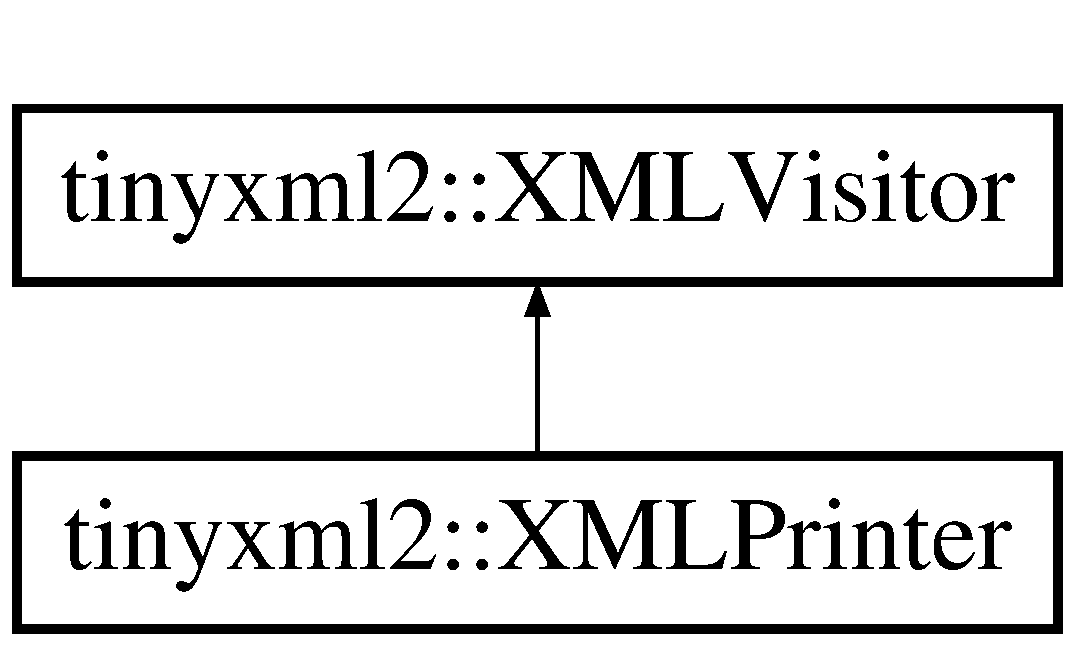
\includegraphics[height=2.000000cm]{classtinyxml2_1_1_x_m_l_visitor}
\end{center}
\end{figure}
\subsection*{Public Member Functions}
\begin{DoxyCompactItemize}
\item 
virtual \hyperlink{classtinyxml2_1_1_x_m_l_visitor_a494e72033d646c47d9c65c502ec62364}{$\sim$\-X\-M\-L\-Visitor} ()
\item 
virtual bool \hyperlink{classtinyxml2_1_1_x_m_l_visitor_acb3c22fc5f60eb9db98f533f2761f67d}{Visit\-Enter} (const \hyperlink{classtinyxml2_1_1_x_m_l_document}{X\-M\-L\-Document} \&)
\begin{DoxyCompactList}\small\item\em Visit a document. \end{DoxyCompactList}\item 
virtual bool \hyperlink{classtinyxml2_1_1_x_m_l_visitor_a170e9989cd046ba904f302d087e07086}{Visit\-Exit} (const \hyperlink{classtinyxml2_1_1_x_m_l_document}{X\-M\-L\-Document} \&)
\begin{DoxyCompactList}\small\item\em Visit a document. \end{DoxyCompactList}\item 
virtual bool \hyperlink{classtinyxml2_1_1_x_m_l_visitor_af97980a17dd4e37448b181f5ddfa92b5}{Visit\-Enter} (const \hyperlink{classtinyxml2_1_1_x_m_l_element}{X\-M\-L\-Element} \&, const \hyperlink{classtinyxml2_1_1_x_m_l_attribute}{X\-M\-L\-Attribute} $\ast$)
\begin{DoxyCompactList}\small\item\em Visit an element. \end{DoxyCompactList}\item 
virtual bool \hyperlink{classtinyxml2_1_1_x_m_l_visitor_a772f10ddc83f881956d32628faa16eb6}{Visit\-Exit} (const \hyperlink{classtinyxml2_1_1_x_m_l_element}{X\-M\-L\-Element} \&)
\begin{DoxyCompactList}\small\item\em Visit an element. \end{DoxyCompactList}\item 
virtual bool \hyperlink{classtinyxml2_1_1_x_m_l_visitor_adc75bd459fc7ba8223b50f0616767f9a}{Visit} (const \hyperlink{classtinyxml2_1_1_x_m_l_declaration}{X\-M\-L\-Declaration} \&)
\begin{DoxyCompactList}\small\item\em Visit a declaration. \end{DoxyCompactList}\item 
virtual bool \hyperlink{classtinyxml2_1_1_x_m_l_visitor_af30233565856480ea48b6fa0d6dec65b}{Visit} (const \hyperlink{classtinyxml2_1_1_x_m_l_text}{X\-M\-L\-Text} \&)
\begin{DoxyCompactList}\small\item\em Visit a text node. \end{DoxyCompactList}\item 
virtual bool \hyperlink{classtinyxml2_1_1_x_m_l_visitor_acc8147fb5a85f6c65721654e427752d7}{Visit} (const \hyperlink{classtinyxml2_1_1_x_m_l_comment}{X\-M\-L\-Comment} \&)
\begin{DoxyCompactList}\small\item\em Visit a comment node. \end{DoxyCompactList}\item 
virtual bool \hyperlink{classtinyxml2_1_1_x_m_l_visitor_a14e4748387c34bf53d24e8119bb1f292}{Visit} (const \hyperlink{classtinyxml2_1_1_x_m_l_unknown}{X\-M\-L\-Unknown} \&)
\begin{DoxyCompactList}\small\item\em Visit an unknown node. \end{DoxyCompactList}\end{DoxyCompactItemize}


\subsection{Detailed Description}
Implements the interface to the \char`\"{}\-Visitor pattern\char`\"{} (see the Accept() method.) If you call the Accept() method, it requires being passed a \hyperlink{classtinyxml2_1_1_x_m_l_visitor}{X\-M\-L\-Visitor} class to handle callbacks. For nodes that contain other nodes (Document, Element) you will get called with a Visit\-Enter/\-Visit\-Exit pair. Nodes that are always leafs are simply called with \hyperlink{classtinyxml2_1_1_x_m_l_visitor_adc75bd459fc7ba8223b50f0616767f9a}{Visit()}.

If you return 'true' from a Visit method, recursive parsing will continue. If you return false, {\bfseries no children of this node or its siblings} will be visited.

All flavors of Visit methods have a default implementation that returns 'true' (continue visiting). You need to only override methods that are interesting to you.

Generally Accept() is called on the \hyperlink{classtinyxml2_1_1_x_m_l_document}{X\-M\-L\-Document}, although all nodes support visiting.

You should never change the document from a callback.

\begin{DoxySeeAlso}{See Also}
\hyperlink{classtinyxml2_1_1_x_m_l_node_a81e66df0a44c67a7af17f3b77a152785}{X\-M\-L\-Node\-::\-Accept()} 
\end{DoxySeeAlso}


\subsection{Constructor \& Destructor Documentation}
\hypertarget{classtinyxml2_1_1_x_m_l_visitor_a494e72033d646c47d9c65c502ec62364}{\index{tinyxml2\-::\-X\-M\-L\-Visitor@{tinyxml2\-::\-X\-M\-L\-Visitor}!$\sim$\-X\-M\-L\-Visitor@{$\sim$\-X\-M\-L\-Visitor}}
\index{$\sim$\-X\-M\-L\-Visitor@{$\sim$\-X\-M\-L\-Visitor}!tinyxml2::XMLVisitor@{tinyxml2\-::\-X\-M\-L\-Visitor}}
\subsubsection[{$\sim$\-X\-M\-L\-Visitor}]{\setlength{\rightskip}{0pt plus 5cm}virtual tinyxml2\-::\-X\-M\-L\-Visitor\-::$\sim$\-X\-M\-L\-Visitor (
\begin{DoxyParamCaption}
{}
\end{DoxyParamCaption}
)\hspace{0.3cm}{\ttfamily [inline]}, {\ttfamily [virtual]}}}\label{classtinyxml2_1_1_x_m_l_visitor_a494e72033d646c47d9c65c502ec62364}


\subsection{Member Function Documentation}
\hypertarget{classtinyxml2_1_1_x_m_l_visitor_adc75bd459fc7ba8223b50f0616767f9a}{\index{tinyxml2\-::\-X\-M\-L\-Visitor@{tinyxml2\-::\-X\-M\-L\-Visitor}!Visit@{Visit}}
\index{Visit@{Visit}!tinyxml2::XMLVisitor@{tinyxml2\-::\-X\-M\-L\-Visitor}}
\subsubsection[{Visit}]{\setlength{\rightskip}{0pt plus 5cm}virtual bool tinyxml2\-::\-X\-M\-L\-Visitor\-::\-Visit (
\begin{DoxyParamCaption}
\item[{const {\bf X\-M\-L\-Declaration} \&}]{}
\end{DoxyParamCaption}
)\hspace{0.3cm}{\ttfamily [inline]}, {\ttfamily [virtual]}}}\label{classtinyxml2_1_1_x_m_l_visitor_adc75bd459fc7ba8223b50f0616767f9a}


Visit a declaration. 



Reimplemented in \hyperlink{classtinyxml2_1_1_x_m_l_printer_acfc625b2549304b9c7eb85ebd5c5eb39}{tinyxml2\-::\-X\-M\-L\-Printer}.

\hypertarget{classtinyxml2_1_1_x_m_l_visitor_af30233565856480ea48b6fa0d6dec65b}{\index{tinyxml2\-::\-X\-M\-L\-Visitor@{tinyxml2\-::\-X\-M\-L\-Visitor}!Visit@{Visit}}
\index{Visit@{Visit}!tinyxml2::XMLVisitor@{tinyxml2\-::\-X\-M\-L\-Visitor}}
\subsubsection[{Visit}]{\setlength{\rightskip}{0pt plus 5cm}virtual bool tinyxml2\-::\-X\-M\-L\-Visitor\-::\-Visit (
\begin{DoxyParamCaption}
\item[{const {\bf X\-M\-L\-Text} \&}]{}
\end{DoxyParamCaption}
)\hspace{0.3cm}{\ttfamily [inline]}, {\ttfamily [virtual]}}}\label{classtinyxml2_1_1_x_m_l_visitor_af30233565856480ea48b6fa0d6dec65b}


Visit a text node. 



Reimplemented in \hyperlink{classtinyxml2_1_1_x_m_l_printer_adc0e42b4f6fcb90a95630c79575d030b}{tinyxml2\-::\-X\-M\-L\-Printer}.

\hypertarget{classtinyxml2_1_1_x_m_l_visitor_acc8147fb5a85f6c65721654e427752d7}{\index{tinyxml2\-::\-X\-M\-L\-Visitor@{tinyxml2\-::\-X\-M\-L\-Visitor}!Visit@{Visit}}
\index{Visit@{Visit}!tinyxml2::XMLVisitor@{tinyxml2\-::\-X\-M\-L\-Visitor}}
\subsubsection[{Visit}]{\setlength{\rightskip}{0pt plus 5cm}virtual bool tinyxml2\-::\-X\-M\-L\-Visitor\-::\-Visit (
\begin{DoxyParamCaption}
\item[{const {\bf X\-M\-L\-Comment} \&}]{}
\end{DoxyParamCaption}
)\hspace{0.3cm}{\ttfamily [inline]}, {\ttfamily [virtual]}}}\label{classtinyxml2_1_1_x_m_l_visitor_acc8147fb5a85f6c65721654e427752d7}


Visit a comment node. 



Reimplemented in \hyperlink{classtinyxml2_1_1_x_m_l_printer_aa294c5c01af0ebb9114902456e4cb53c}{tinyxml2\-::\-X\-M\-L\-Printer}.

\hypertarget{classtinyxml2_1_1_x_m_l_visitor_a14e4748387c34bf53d24e8119bb1f292}{\index{tinyxml2\-::\-X\-M\-L\-Visitor@{tinyxml2\-::\-X\-M\-L\-Visitor}!Visit@{Visit}}
\index{Visit@{Visit}!tinyxml2::XMLVisitor@{tinyxml2\-::\-X\-M\-L\-Visitor}}
\subsubsection[{Visit}]{\setlength{\rightskip}{0pt plus 5cm}virtual bool tinyxml2\-::\-X\-M\-L\-Visitor\-::\-Visit (
\begin{DoxyParamCaption}
\item[{const {\bf X\-M\-L\-Unknown} \&}]{}
\end{DoxyParamCaption}
)\hspace{0.3cm}{\ttfamily [inline]}, {\ttfamily [virtual]}}}\label{classtinyxml2_1_1_x_m_l_visitor_a14e4748387c34bf53d24e8119bb1f292}


Visit an unknown node. 



Reimplemented in \hyperlink{classtinyxml2_1_1_x_m_l_printer_ab8af5455bbf9e4be2663e6642fcd7e32}{tinyxml2\-::\-X\-M\-L\-Printer}.

\hypertarget{classtinyxml2_1_1_x_m_l_visitor_acb3c22fc5f60eb9db98f533f2761f67d}{\index{tinyxml2\-::\-X\-M\-L\-Visitor@{tinyxml2\-::\-X\-M\-L\-Visitor}!Visit\-Enter@{Visit\-Enter}}
\index{Visit\-Enter@{Visit\-Enter}!tinyxml2::XMLVisitor@{tinyxml2\-::\-X\-M\-L\-Visitor}}
\subsubsection[{Visit\-Enter}]{\setlength{\rightskip}{0pt plus 5cm}virtual bool tinyxml2\-::\-X\-M\-L\-Visitor\-::\-Visit\-Enter (
\begin{DoxyParamCaption}
\item[{const {\bf X\-M\-L\-Document} \&}]{}
\end{DoxyParamCaption}
)\hspace{0.3cm}{\ttfamily [inline]}, {\ttfamily [virtual]}}}\label{classtinyxml2_1_1_x_m_l_visitor_acb3c22fc5f60eb9db98f533f2761f67d}


Visit a document. 



Reimplemented in \hyperlink{classtinyxml2_1_1_x_m_l_printer_a9aa1de11a55a07db55a90fde37d7afad}{tinyxml2\-::\-X\-M\-L\-Printer}.

\hypertarget{classtinyxml2_1_1_x_m_l_visitor_af97980a17dd4e37448b181f5ddfa92b5}{\index{tinyxml2\-::\-X\-M\-L\-Visitor@{tinyxml2\-::\-X\-M\-L\-Visitor}!Visit\-Enter@{Visit\-Enter}}
\index{Visit\-Enter@{Visit\-Enter}!tinyxml2::XMLVisitor@{tinyxml2\-::\-X\-M\-L\-Visitor}}
\subsubsection[{Visit\-Enter}]{\setlength{\rightskip}{0pt plus 5cm}virtual bool tinyxml2\-::\-X\-M\-L\-Visitor\-::\-Visit\-Enter (
\begin{DoxyParamCaption}
\item[{const {\bf X\-M\-L\-Element} \&}]{, }
\item[{const {\bf X\-M\-L\-Attribute} $\ast$}]{}
\end{DoxyParamCaption}
)\hspace{0.3cm}{\ttfamily [inline]}, {\ttfamily [virtual]}}}\label{classtinyxml2_1_1_x_m_l_visitor_af97980a17dd4e37448b181f5ddfa92b5}


Visit an element. 



Reimplemented in \hyperlink{classtinyxml2_1_1_x_m_l_printer_a169b2509d8eabb70811b2bb8cfd1f5d1}{tinyxml2\-::\-X\-M\-L\-Printer}.

\hypertarget{classtinyxml2_1_1_x_m_l_visitor_a170e9989cd046ba904f302d087e07086}{\index{tinyxml2\-::\-X\-M\-L\-Visitor@{tinyxml2\-::\-X\-M\-L\-Visitor}!Visit\-Exit@{Visit\-Exit}}
\index{Visit\-Exit@{Visit\-Exit}!tinyxml2::XMLVisitor@{tinyxml2\-::\-X\-M\-L\-Visitor}}
\subsubsection[{Visit\-Exit}]{\setlength{\rightskip}{0pt plus 5cm}virtual bool tinyxml2\-::\-X\-M\-L\-Visitor\-::\-Visit\-Exit (
\begin{DoxyParamCaption}
\item[{const {\bf X\-M\-L\-Document} \&}]{}
\end{DoxyParamCaption}
)\hspace{0.3cm}{\ttfamily [inline]}, {\ttfamily [virtual]}}}\label{classtinyxml2_1_1_x_m_l_visitor_a170e9989cd046ba904f302d087e07086}


Visit a document. 



Reimplemented in \hyperlink{classtinyxml2_1_1_x_m_l_printer_a15fc1f2b922f540917dcf52808737b29}{tinyxml2\-::\-X\-M\-L\-Printer}.

\hypertarget{classtinyxml2_1_1_x_m_l_visitor_a772f10ddc83f881956d32628faa16eb6}{\index{tinyxml2\-::\-X\-M\-L\-Visitor@{tinyxml2\-::\-X\-M\-L\-Visitor}!Visit\-Exit@{Visit\-Exit}}
\index{Visit\-Exit@{Visit\-Exit}!tinyxml2::XMLVisitor@{tinyxml2\-::\-X\-M\-L\-Visitor}}
\subsubsection[{Visit\-Exit}]{\setlength{\rightskip}{0pt plus 5cm}virtual bool tinyxml2\-::\-X\-M\-L\-Visitor\-::\-Visit\-Exit (
\begin{DoxyParamCaption}
\item[{const {\bf X\-M\-L\-Element} \&}]{}
\end{DoxyParamCaption}
)\hspace{0.3cm}{\ttfamily [inline]}, {\ttfamily [virtual]}}}\label{classtinyxml2_1_1_x_m_l_visitor_a772f10ddc83f881956d32628faa16eb6}


Visit an element. 



Reimplemented in \hyperlink{classtinyxml2_1_1_x_m_l_printer_a2edd48405971a88951c71c9df86a2f50}{tinyxml2\-::\-X\-M\-L\-Printer}.



The documentation for this class was generated from the following file\-:\begin{DoxyCompactItemize}
\item 
Utils/\-X\-M\-L\-\_\-\-Config/\hyperlink{tinyxml2_8h}{tinyxml2.\-h}\end{DoxyCompactItemize}

\chapter{File Documentation}
\hypertarget{_command_8h}{\section{Base/\-Command.h File Reference}
\label{_command_8h}\index{Base/\-Command.\-h@{Base/\-Command.\-h}}
}
{\ttfamily \#include \char`\"{}Event.\-h\char`\"{}}\\*
\subsection*{Classes}
\begin{DoxyCompactItemize}
\item 
class \hyperlink{classn8_1_1_command}{n8\-::\-Command}
\end{DoxyCompactItemize}
\subsection*{Namespaces}
\begin{DoxyCompactItemize}
\item 
\hyperlink{namespacen8}{n8}
\end{DoxyCompactItemize}
\subsection*{Constant Groups}
\begin{DoxyCompactItemize}
\item 
\hyperlink{namespacen8}{n8}
\end{DoxyCompactItemize}

\hypertarget{_i_d_8h}{\section{Base/\-I\-D.h File Reference}
\label{_i_d_8h}\index{Base/\-I\-D.\-h@{Base/\-I\-D.\-h}}
}
{\ttfamily \#include $<$iostream$>$}\\*
\subsection*{Classes}
\begin{DoxyCompactItemize}
\item 
class \hyperlink{class_i_d}{I\-D}
\end{DoxyCompactItemize}

\hypertarget{_object_factory_8cpp}{\section{Base/\-Object\-Factory.cpp File Reference}
\label{_object_factory_8cpp}\index{Base/\-Object\-Factory.\-cpp@{Base/\-Object\-Factory.\-cpp}}
}
{\ttfamily \#include \char`\"{}Object\-Factory.\-h\char`\"{}}\\*

\hypertarget{_object_factory_8h}{\section{Base/\-Object\-Factory.h File Reference}
\label{_object_factory_8h}\index{Base/\-Object\-Factory.\-h@{Base/\-Object\-Factory.\-h}}
}
{\ttfamily \#include $<$iostream$>$}\\*
\subsection*{Classes}
\begin{DoxyCompactItemize}
\item 
class \hyperlink{classn8_1_1_object_factory}{n8\-::\-Object\-Factory}
\end{DoxyCompactItemize}
\subsection*{Namespaces}
\begin{DoxyCompactItemize}
\item 
\hyperlink{namespacen8}{n8}
\end{DoxyCompactItemize}
\subsection*{Constant Groups}
\begin{DoxyCompactItemize}
\item 
\hyperlink{namespacen8}{n8}
\end{DoxyCompactItemize}

\hypertarget{_resource_8h}{\section{Base/\-Resource.h File Reference}
\label{_resource_8h}\index{Base/\-Resource.\-h@{Base/\-Resource.\-h}}
}
{\ttfamily \#include $<$string$>$}\\*
{\ttfamily \#include \char`\"{}S\-D\-L2/\-S\-D\-L.\-h\char`\"{}}\\*
{\ttfamily \#include \char`\"{}S\-D\-L2\-\_\-image/\-S\-D\-L\-\_\-image.\-h\char`\"{}}\\*
{\ttfamily \#include \char`\"{}S\-D\-L2\-\_\-mixer/\-S\-D\-L\-\_\-mixer.\-h\char`\"{}}\\*
{\ttfamily \#include \char`\"{}S\-D\-L2\-\_\-ttf/\-S\-D\-L\-\_\-ttf.\-h\char`\"{}}\\*
\subsection*{Classes}
\begin{DoxyCompactItemize}
\item 
class \hyperlink{classn8_1_1_resource}{n8\-::\-Resource}
\end{DoxyCompactItemize}
\subsection*{Namespaces}
\begin{DoxyCompactItemize}
\item 
\hyperlink{namespacen8}{n8}
\end{DoxyCompactItemize}
\subsection*{Constant Groups}
\begin{DoxyCompactItemize}
\item 
\hyperlink{namespacen8}{n8}
\end{DoxyCompactItemize}

\hypertarget{_service_8cpp}{\section{Base/\-Service.cpp File Reference}
\label{_service_8cpp}\index{Base/\-Service.\-cpp@{Base/\-Service.\-cpp}}
}
{\ttfamily \#include \char`\"{}Service.\-h\char`\"{}}\\*

\hypertarget{_service_8h}{\section{Base/\-Service.h File Reference}
\label{_service_8h}\index{Base/\-Service.\-h@{Base/\-Service.\-h}}
}
{\ttfamily \#include $<$iostream$>$}\\*
{\ttfamily \#include $<$map$>$}\\*
{\ttfamily \#include \char`\"{}../\-Core/\-Enums.\-h\char`\"{}}\\*
{\ttfamily \#include \char`\"{}Observer.\-h\char`\"{}}\\*
{\ttfamily \#include \char`\"{}Subject.\-h\char`\"{}}\\*
\subsection*{Classes}
\begin{DoxyCompactItemize}
\item 
class \hyperlink{classn8_1_1_service}{n8\-::\-Service}
\end{DoxyCompactItemize}
\subsection*{Namespaces}
\begin{DoxyCompactItemize}
\item 
\hyperlink{namespacen8}{n8}
\end{DoxyCompactItemize}
\subsection*{Constant Groups}
\begin{DoxyCompactItemize}
\item 
\hyperlink{namespacen8}{n8}
\end{DoxyCompactItemize}

\hypertarget{_singleton_8h}{\section{Base/\-Singleton.h File Reference}
\label{_singleton_8h}\index{Base/\-Singleton.\-h@{Base/\-Singleton.\-h}}
}
{\ttfamily \#include $<$iostream$>$}\\*
{\ttfamily \#include $<$assert.\-h$>$}\\*
\subsection*{Classes}
\begin{DoxyCompactItemize}
\item 
class \hyperlink{class_singleton}{Singleton$<$ T $>$}
\end{DoxyCompactItemize}

\hypertarget{_state_8h}{\section{Base/\-State.h File Reference}
\label{_state_8h}\index{Base/\-State.\-h@{Base/\-State.\-h}}
}
{\ttfamily \#include $<$iostream$>$}\\*
{\ttfamily \#include $<$vector$>$}\\*
{\ttfamily \#include $<$assert.\-h$>$}\\*
{\ttfamily \#include \char`\"{}S\-D\-L2/\-S\-D\-L.\-h\char`\"{}}\\*
{\ttfamily \#include \char`\"{}S\-D\-L2\-\_\-image/\-S\-D\-L\-\_\-image.\-h\char`\"{}}\\*
{\ttfamily \#include \char`\"{}I\-D.\-h\char`\"{}}\\*
\subsection*{Classes}
\begin{DoxyCompactItemize}
\item 
class \hyperlink{classn8_1_1_state}{n8\-::\-State}
\end{DoxyCompactItemize}
\subsection*{Namespaces}
\begin{DoxyCompactItemize}
\item 
\hyperlink{namespacen8}{n8}
\end{DoxyCompactItemize}
\subsection*{Constant Groups}
\begin{DoxyCompactItemize}
\item 
\hyperlink{namespacen8}{n8}
\end{DoxyCompactItemize}

\hypertarget{_pop_state_command_8cpp}{\section{Commands/\-Pop\-State\-Command.cpp File Reference}
\label{_pop_state_command_8cpp}\index{Commands/\-Pop\-State\-Command.\-cpp@{Commands/\-Pop\-State\-Command.\-cpp}}
}
{\ttfamily \#include \char`\"{}Pop\-State\-Command.\-h\char`\"{}}\\*

\hypertarget{_pop_state_command_8h}{\section{Commands/\-Pop\-State\-Command.h File Reference}
\label{_pop_state_command_8h}\index{Commands/\-Pop\-State\-Command.\-h@{Commands/\-Pop\-State\-Command.\-h}}
}
{\ttfamily \#include $<$iostream$>$}\\*
{\ttfamily \#include \char`\"{}Command.\-h\char`\"{}}\\*
{\ttfamily \#include \char`\"{}State\-Manager\-Service.\-h\char`\"{}}\\*
{\ttfamily \#include \char`\"{}Service\-Manager.\-h\char`\"{}}\\*
\subsection*{Classes}
\begin{DoxyCompactItemize}
\item 
class \hyperlink{classn8_1_1_pop_state_command}{n8\-::\-Pop\-State\-Command}
\end{DoxyCompactItemize}
\subsection*{Namespaces}
\begin{DoxyCompactItemize}
\item 
\hyperlink{namespacen8}{n8}
\end{DoxyCompactItemize}
\subsection*{Constant Groups}
\begin{DoxyCompactItemize}
\item 
\hyperlink{namespacen8}{n8}
\end{DoxyCompactItemize}

\hypertarget{_push_state_command_8cpp}{\section{Commands/\-Push\-State\-Command.cpp File Reference}
\label{_push_state_command_8cpp}\index{Commands/\-Push\-State\-Command.\-cpp@{Commands/\-Push\-State\-Command.\-cpp}}
}
{\ttfamily \#include \char`\"{}Push\-State\-Command.\-h\char`\"{}}\\*

\hypertarget{_push_state_command_8h}{\section{Commands/\-Push\-State\-Command.h File Reference}
\label{_push_state_command_8h}\index{Commands/\-Push\-State\-Command.\-h@{Commands/\-Push\-State\-Command.\-h}}
}
{\ttfamily \#include $<$iostream$>$}\\*
{\ttfamily \#include \char`\"{}Command.\-h\char`\"{}}\\*
{\ttfamily \#include \char`\"{}State\-Manager\-Service.\-h\char`\"{}}\\*
{\ttfamily \#include \char`\"{}Service\-Manager.\-h\char`\"{}}\\*
{\ttfamily \#include \char`\"{}Enums.\-h\char`\"{}}\\*
\subsection*{Classes}
\begin{DoxyCompactItemize}
\item 
class \hyperlink{classn8_1_1_push_state_command}{n8\-::\-Push\-State\-Command}
\end{DoxyCompactItemize}
\subsection*{Namespaces}
\begin{DoxyCompactItemize}
\item 
\hyperlink{namespacen8}{n8}
\end{DoxyCompactItemize}
\subsection*{Constant Groups}
\begin{DoxyCompactItemize}
\item 
\hyperlink{namespacen8}{n8}
\end{DoxyCompactItemize}

\hypertarget{_event_8cpp}{\section{Communication/\-Event.cpp File Reference}
\label{_event_8cpp}\index{Communication/\-Event.\-cpp@{Communication/\-Event.\-cpp}}
}
{\ttfamily \#include \char`\"{}Event.\-h\char`\"{}}\\*

\hypertarget{_event_8h}{\section{Communication/\-Event.h File Reference}
\label{_event_8h}\index{Communication/\-Event.\-h@{Communication/\-Event.\-h}}
}
{\ttfamily \#include $<$iostream$>$}\\*
{\ttfamily \#include \char`\"{}../\-Core/\-Enums.\-h\char`\"{}}\\*
\subsection*{Classes}
\begin{DoxyCompactItemize}
\item 
class \hyperlink{classn8_1_1_event}{n8\-::\-Event}
\end{DoxyCompactItemize}
\subsection*{Namespaces}
\begin{DoxyCompactItemize}
\item 
\hyperlink{namespacen8}{n8}
\end{DoxyCompactItemize}
\subsection*{Constant Groups}
\begin{DoxyCompactItemize}
\item 
\hyperlink{namespacen8}{n8}
\end{DoxyCompactItemize}

\hypertarget{_observer_8cpp}{\section{Communication/\-Observer.cpp File Reference}
\label{_observer_8cpp}\index{Communication/\-Observer.\-cpp@{Communication/\-Observer.\-cpp}}
}
{\ttfamily \#include \char`\"{}Observer.\-h\char`\"{}}\\*

\hypertarget{_observer_8h}{\section{Communication/\-Observer.h File Reference}
\label{_observer_8h}\index{Communication/\-Observer.\-h@{Communication/\-Observer.\-h}}
}
{\ttfamily \#include $<$iostream$>$}\\*
{\ttfamily \#include \char`\"{}Event.\-h\char`\"{}}\\*
\subsection*{Classes}
\begin{DoxyCompactItemize}
\item 
class \hyperlink{classn8_1_1_observer}{n8\-::\-Observer}
\end{DoxyCompactItemize}
\subsection*{Namespaces}
\begin{DoxyCompactItemize}
\item 
\hyperlink{namespacen8}{n8}
\end{DoxyCompactItemize}
\subsection*{Constant Groups}
\begin{DoxyCompactItemize}
\item 
\hyperlink{namespacen8}{n8}
\end{DoxyCompactItemize}

\hypertarget{_subject_8cpp}{\section{Communication/\-Subject.cpp File Reference}
\label{_subject_8cpp}\index{Communication/\-Subject.\-cpp@{Communication/\-Subject.\-cpp}}
}
{\ttfamily \#include \char`\"{}Subject.\-h\char`\"{}}\\*

\hypertarget{_subject_8h}{\section{Communication/\-Subject.h File Reference}
\label{_subject_8h}\index{Communication/\-Subject.\-h@{Communication/\-Subject.\-h}}
}
{\ttfamily \#include $<$iostream$>$}\\*
{\ttfamily \#include $<$vector$>$}\\*
{\ttfamily \#include \char`\"{}Observer.\-h\char`\"{}}\\*
{\ttfamily \#include \char`\"{}Event.\-h\char`\"{}}\\*
\subsection*{Classes}
\begin{DoxyCompactItemize}
\item 
class \hyperlink{classn8_1_1_subject}{n8\-::\-Subject}
\end{DoxyCompactItemize}
\subsection*{Namespaces}
\begin{DoxyCompactItemize}
\item 
\hyperlink{namespacen8}{n8}
\end{DoxyCompactItemize}
\subsection*{Constant Groups}
\begin{DoxyCompactItemize}
\item 
\hyperlink{namespacen8}{n8}
\end{DoxyCompactItemize}

\hypertarget{_enums_8h}{\section{Core/\-Enums.h File Reference}
\label{_enums_8h}\index{Core/\-Enums.\-h@{Core/\-Enums.\-h}}
}
\subsection*{Namespaces}
\begin{DoxyCompactItemize}
\item 
\hyperlink{namespace_e_color}{E\-Color}
\item 
\hyperlink{namespace_e_service}{E\-Service}
\item 
\hyperlink{namespace_e_state}{E\-State}
\item 
\hyperlink{namespace_e_events}{E\-Events}
\end{DoxyCompactItemize}
\subsection*{Constant Groups}
\begin{DoxyCompactItemize}
\item 
\hyperlink{namespace_e_color}{E\-Color}
\item 
\hyperlink{namespace_e_service}{E\-Service}
\item 
\hyperlink{namespace_e_state}{E\-State}
\item 
\hyperlink{namespace_e_events}{E\-Events}
\end{DoxyCompactItemize}
\subsection*{Enumerations}
\begin{DoxyCompactItemize}
\item 
enum \hyperlink{namespace_e_color_a1d097defd7361c72d8e6081bcd9a77da}{E\-Color\-::\-Values} \{ \hyperlink{namespace_e_color_a1d097defd7361c72d8e6081bcd9a77daa0297846ca926ea253d1f471eea8a26fe}{E\-Color\-::\-Red}, 
\hyperlink{namespace_e_color_a1d097defd7361c72d8e6081bcd9a77daa03a2249c2b34a64fd74600d0944d0e1f}{E\-Color\-::\-Green}, 
\hyperlink{namespace_e_color_a1d097defd7361c72d8e6081bcd9a77daae81f4bff75606d265b5063c235b6cd48}{E\-Color\-::\-Blue}
 \}
\item 
enum \hyperlink{namespace_e_service_a7d0bb3de6ea857dc1253fc5a2cef6884}{E\-Service\-::\-Values} \{ \\*
\hyperlink{namespace_e_service_a7d0bb3de6ea857dc1253fc5a2cef6884aaa0c6ca39b12c98963feccbf24d1125e}{E\-Service\-::\-Input}, 
\hyperlink{namespace_e_service_a7d0bb3de6ea857dc1253fc5a2cef6884af8fb8c8e8ba7ebade4d641878dd6bd80}{E\-Service\-::\-Resources}, 
\hyperlink{namespace_e_service_a7d0bb3de6ea857dc1253fc5a2cef6884a5cafde5fd65dca03221f9b2d151e94ab}{E\-Service\-::\-State\-Manager}, 
\hyperlink{namespace_e_service_a7d0bb3de6ea857dc1253fc5a2cef6884a23a6ae22440514fed3b057273d70239c}{E\-Service\-::\-Render}, 
\\*
\hyperlink{namespace_e_service_a7d0bb3de6ea857dc1253fc5a2cef6884a99e083bf32988467af021670a7c3ab63}{E\-Service\-::\-Audio}, 
\hyperlink{namespace_e_service_a7d0bb3de6ea857dc1253fc5a2cef6884a132e5220105ebc80e23cfcc01f61a68c}{E\-Service\-::\-Logging}, 
\hyperlink{namespace_e_service_a7d0bb3de6ea857dc1253fc5a2cef6884a76b185527da9e0f5397b667f3a8539d8}{E\-Service\-::\-A\-I}
 \}
\item 
enum \hyperlink{namespace_e_state_aee586325ec9fecd1205d41439870dd81}{E\-State\-::\-Values} \{ \hyperlink{namespace_e_state_aee586325ec9fecd1205d41439870dd81ade06ddf13aacb666de00b3a57f8b1896}{E\-State\-::\-Test}, 
\hyperlink{namespace_e_state_aee586325ec9fecd1205d41439870dd81af843c6723c33e92075e2a9b925862381}{E\-State\-::\-Test2}
 \}
\item 
enum \hyperlink{namespace_e_events_ad7951ce20842f9eeb617fae73d4c9504}{E\-Events\-::\-Values} \{ \hyperlink{namespace_e_events_ad7951ce20842f9eeb617fae73d4c9504a20233e366b9f50a1f82ff8da569d787d}{E\-Events\-::\-Exit}, 
\hyperlink{namespace_e_events_ad7951ce20842f9eeb617fae73d4c9504ae1a9c86642a36392472af0e7faa00d24}{E\-Events\-::\-Test2}
 \}
\end{DoxyCompactItemize}

\hypertarget{_game_8cpp}{\section{Core/\-Game.cpp File Reference}
\label{_game_8cpp}\index{Core/\-Game.\-cpp@{Core/\-Game.\-cpp}}
}
{\ttfamily \#include $<$assert.\-h$>$}\\*
{\ttfamily \#include \char`\"{}Game.\-h\char`\"{}}\\*
\subsection*{Macros}
\begin{DoxyCompactItemize}
\item 
\#define \hyperlink{_game_8cpp_afc3d101f633a076cc1ca84b85b6224b2}{T\-A\-G}~\char`\"{}Game\char`\"{}
\end{DoxyCompactItemize}


\subsection{Macro Definition Documentation}
\hypertarget{_game_8cpp_afc3d101f633a076cc1ca84b85b6224b2}{\index{Game.\-cpp@{Game.\-cpp}!T\-A\-G@{T\-A\-G}}
\index{T\-A\-G@{T\-A\-G}!Game.cpp@{Game.\-cpp}}
\subsubsection[{T\-A\-G}]{\setlength{\rightskip}{0pt plus 5cm}\#define T\-A\-G~\char`\"{}Game\char`\"{}}}\label{_game_8cpp_afc3d101f633a076cc1ca84b85b6224b2}

\hypertarget{_game_8h}{\section{Core/\-Game.h File Reference}
\label{_game_8h}\index{Core/\-Game.\-h@{Core/\-Game.\-h}}
}
{\ttfamily \#include $<$iostream$>$}\\*
{\ttfamily \#include $<$S\-D\-L2/\-S\-D\-L.\-h$>$}\\*
{\ttfamily \#include \char`\"{}S\-D\-L2\-\_\-image/\-S\-D\-L\-\_\-image.\-h\char`\"{}}\\*
{\ttfamily \#include \char`\"{}S\-D\-L2\-\_\-mixer/\-S\-D\-L\-\_\-mixer.\-h\char`\"{}}\\*
{\ttfamily \#include \char`\"{}S\-D\-L2\-\_\-ttf/\-S\-D\-L\-\_\-ttf.\-h\char`\"{}}\\*
{\ttfamily \#include \char`\"{}tinyxml2.\-h\char`\"{}}\\*
{\ttfamily \#include \char`\"{}Service\-Manager.\-h\char`\"{}}\\*
{\ttfamily \#include \char`\"{}Log.\-h\char`\"{}}\\*
{\ttfamily \#include \char`\"{}Input\-Service.\-h\char`\"{}}\\*
{\ttfamily \#include \char`\"{}State\-Manager\-Service.\-h\char`\"{}}\\*
{\ttfamily \#include \char`\"{}Resource\-Manager.\-h\char`\"{}}\\*
{\ttfamily \#include \char`\"{}State.\-h\char`\"{}}\\*
{\ttfamily \#include \char`\"{}Timer.\-h\char`\"{}}\\*
{\ttfamily \#include \char`\"{}Window.\-h\char`\"{}}\\*
\subsection*{Classes}
\begin{DoxyCompactItemize}
\item 
class \hyperlink{classn8_1_1_game}{n8\-::\-Game}
\end{DoxyCompactItemize}
\subsection*{Namespaces}
\begin{DoxyCompactItemize}
\item 
\hyperlink{namespacen8}{n8}
\end{DoxyCompactItemize}
\subsection*{Constant Groups}
\begin{DoxyCompactItemize}
\item 
\hyperlink{namespacen8}{n8}
\end{DoxyCompactItemize}

\hypertarget{_service_manager_8cpp}{\section{Core/\-Service\-Manager.cpp File Reference}
\label{_service_manager_8cpp}\index{Core/\-Service\-Manager.\-cpp@{Core/\-Service\-Manager.\-cpp}}
}
{\ttfamily \#include \char`\"{}Service\-Manager.\-h\char`\"{}}\\*
{\ttfamily \#include \char`\"{}Log.\-h\char`\"{}}\\*
\subsection*{Macros}
\begin{DoxyCompactItemize}
\item 
\#define \hyperlink{_service_manager_8cpp_afc3d101f633a076cc1ca84b85b6224b2}{T\-A\-G}~\char`\"{}Service\-Manager\char`\"{}
\end{DoxyCompactItemize}


\subsection{Macro Definition Documentation}
\hypertarget{_service_manager_8cpp_afc3d101f633a076cc1ca84b85b6224b2}{\index{Service\-Manager.\-cpp@{Service\-Manager.\-cpp}!T\-A\-G@{T\-A\-G}}
\index{T\-A\-G@{T\-A\-G}!ServiceManager.cpp@{Service\-Manager.\-cpp}}
\subsubsection[{T\-A\-G}]{\setlength{\rightskip}{0pt plus 5cm}\#define T\-A\-G~\char`\"{}Service\-Manager\char`\"{}}}\label{_service_manager_8cpp_afc3d101f633a076cc1ca84b85b6224b2}

\hypertarget{_service_manager_8h}{\section{Core/\-Service\-Manager.h File Reference}
\label{_service_manager_8h}\index{Core/\-Service\-Manager.\-h@{Core/\-Service\-Manager.\-h}}
}
{\ttfamily \#include $<$iostream$>$}\\*
{\ttfamily \#include $<$map$>$}\\*
{\ttfamily \#include \char`\"{}Singleton.\-h\char`\"{}}\\*
{\ttfamily \#include \char`\"{}Service.\-h\char`\"{}}\\*
{\ttfamily \#include \char`\"{}../\-Core/\-Enums.\-h\char`\"{}}\\*
\subsection*{Classes}
\begin{DoxyCompactItemize}
\item 
class \hyperlink{classn8_1_1_service_manager}{n8\-::\-Service\-Manager}
\end{DoxyCompactItemize}
\subsection*{Namespaces}
\begin{DoxyCompactItemize}
\item 
\hyperlink{namespacen8}{n8}
\end{DoxyCompactItemize}
\subsection*{Constant Groups}
\begin{DoxyCompactItemize}
\item 
\hyperlink{namespacen8}{n8}
\end{DoxyCompactItemize}

\hypertarget{_timer_8cpp}{\section{Core/\-Timer.cpp File Reference}
\label{_timer_8cpp}\index{Core/\-Timer.\-cpp@{Core/\-Timer.\-cpp}}
}
{\ttfamily \#include \char`\"{}Timer.\-h\char`\"{}}\\*

\hypertarget{_timer_8h}{\section{Core/\-Timer.h File Reference}
\label{_timer_8h}\index{Core/\-Timer.\-h@{Core/\-Timer.\-h}}
}
{\ttfamily \#include $<$iostream$>$}\\*
{\ttfamily \#include \char`\"{}S\-D\-L2/\-S\-D\-L.\-h\char`\"{}}\\*
\subsection*{Classes}
\begin{DoxyCompactItemize}
\item 
class \hyperlink{classn8_1_1_timer}{n8\-::\-Timer}
\end{DoxyCompactItemize}
\subsection*{Namespaces}
\begin{DoxyCompactItemize}
\item 
\hyperlink{namespacen8}{n8}
\end{DoxyCompactItemize}
\subsection*{Constant Groups}
\begin{DoxyCompactItemize}
\item 
\hyperlink{namespacen8}{n8}
\end{DoxyCompactItemize}

\hypertarget{_window_8cpp}{\section{Core/\-Window.cpp File Reference}
\label{_window_8cpp}\index{Core/\-Window.\-cpp@{Core/\-Window.\-cpp}}
}
{\ttfamily \#include $<$assert.\-h$>$}\\*
{\ttfamily \#include \char`\"{}Window.\-h\char`\"{}}\\*
{\ttfamily \#include \char`\"{}Service\-Manager.\-h\char`\"{}}\\*
{\ttfamily \#include \char`\"{}Log.\-h\char`\"{}}\\*

\hypertarget{_window_8h}{\section{Core/\-Window.h File Reference}
\label{_window_8h}\index{Core/\-Window.\-h@{Core/\-Window.\-h}}
}
{\ttfamily \#include $<$iostream$>$}\\*
{\ttfamily \#include \char`\"{}S\-D\-L2/\-S\-D\-L.\-h\char`\"{}}\\*
{\ttfamily \#include \char`\"{}S\-D\-L2\-\_\-image/\-S\-D\-L\-\_\-image.\-h\char`\"{}}\\*
\subsection*{Classes}
\begin{DoxyCompactItemize}
\item 
class \hyperlink{classn8_1_1_window}{n8\-::\-Window}
\end{DoxyCompactItemize}
\subsection*{Namespaces}
\begin{DoxyCompactItemize}
\item 
\hyperlink{namespacen8}{n8}
\end{DoxyCompactItemize}
\subsection*{Constant Groups}
\begin{DoxyCompactItemize}
\item 
\hyperlink{namespacen8}{n8}
\end{DoxyCompactItemize}

\hypertarget{_font_8cpp}{\section{Resources/\-Font.cpp File Reference}
\label{_font_8cpp}\index{Resources/\-Font.\-cpp@{Resources/\-Font.\-cpp}}
}
{\ttfamily \#include \char`\"{}Font.\-h\char`\"{}}\\*

\hypertarget{_font_8h}{\section{Resources/\-Font.h File Reference}
\label{_font_8h}\index{Resources/\-Font.\-h@{Resources/\-Font.\-h}}
}
{\ttfamily \#include $<$iostream$>$}\\*
{\ttfamily \#include $<$string$>$}\\*
{\ttfamily \#include \char`\"{}Resource.\-h\char`\"{}}\\*
\subsection*{Classes}
\begin{DoxyCompactItemize}
\item 
class \hyperlink{classn8_1_1_font}{n8\-::\-Font}
\end{DoxyCompactItemize}
\subsection*{Namespaces}
\begin{DoxyCompactItemize}
\item 
\hyperlink{namespacen8}{n8}
\end{DoxyCompactItemize}
\subsection*{Constant Groups}
\begin{DoxyCompactItemize}
\item 
\hyperlink{namespacen8}{n8}
\end{DoxyCompactItemize}

\hypertarget{_music_8cpp}{\section{Resources/\-Music.cpp File Reference}
\label{_music_8cpp}\index{Resources/\-Music.\-cpp@{Resources/\-Music.\-cpp}}
}
{\ttfamily \#include \char`\"{}Music.\-h\char`\"{}}\\*

\hypertarget{_music_8h}{\section{Resources/\-Music.h File Reference}
\label{_music_8h}\index{Resources/\-Music.\-h@{Resources/\-Music.\-h}}
}
{\ttfamily \#include $<$iostream$>$}\\*
{\ttfamily \#include $<$string$>$}\\*
{\ttfamily \#include \char`\"{}Resource.\-h\char`\"{}}\\*
\subsection*{Classes}
\begin{DoxyCompactItemize}
\item 
class \hyperlink{classn8_1_1_music}{n8\-::\-Music}
\end{DoxyCompactItemize}
\subsection*{Namespaces}
\begin{DoxyCompactItemize}
\item 
\hyperlink{namespacen8}{n8}
\end{DoxyCompactItemize}
\subsection*{Constant Groups}
\begin{DoxyCompactItemize}
\item 
\hyperlink{namespacen8}{n8}
\end{DoxyCompactItemize}

\hypertarget{_sound_effect_8cpp}{\section{Resources/\-Sound\-Effect.cpp File Reference}
\label{_sound_effect_8cpp}\index{Resources/\-Sound\-Effect.\-cpp@{Resources/\-Sound\-Effect.\-cpp}}
}
{\ttfamily \#include \char`\"{}Sound\-Effect.\-h\char`\"{}}\\*

\hypertarget{_sound_effect_8h}{\section{Resources/\-Sound\-Effect.h File Reference}
\label{_sound_effect_8h}\index{Resources/\-Sound\-Effect.\-h@{Resources/\-Sound\-Effect.\-h}}
}
{\ttfamily \#include $<$iostream$>$}\\*
{\ttfamily \#include $<$string$>$}\\*
{\ttfamily \#include \char`\"{}Resource.\-h\char`\"{}}\\*
\subsection*{Classes}
\begin{DoxyCompactItemize}
\item 
class \hyperlink{classn8_1_1_sound_effect}{n8\-::\-Sound\-Effect}
\end{DoxyCompactItemize}
\subsection*{Namespaces}
\begin{DoxyCompactItemize}
\item 
\hyperlink{namespacen8}{n8}
\end{DoxyCompactItemize}
\subsection*{Constant Groups}
\begin{DoxyCompactItemize}
\item 
\hyperlink{namespacen8}{n8}
\end{DoxyCompactItemize}

\hypertarget{_sprite_8cpp}{\section{Resources/\-Sprite.cpp File Reference}
\label{_sprite_8cpp}\index{Resources/\-Sprite.\-cpp@{Resources/\-Sprite.\-cpp}}
}
{\ttfamily \#include \char`\"{}Sprite.\-h\char`\"{}}\\*
{\ttfamily \#include $<$assert.\-h$>$}\\*
\subsection*{Namespaces}
\begin{DoxyCompactItemize}
\item 
\hyperlink{namespacen8}{n8}
\end{DoxyCompactItemize}
\subsection*{Constant Groups}
\begin{DoxyCompactItemize}
\item 
\hyperlink{namespacen8}{n8}
\end{DoxyCompactItemize}

\hypertarget{_sprite_8h}{\section{Resources/\-Sprite.h File Reference}
\label{_sprite_8h}\index{Resources/\-Sprite.\-h@{Resources/\-Sprite.\-h}}
}
{\ttfamily \#include $<$string$>$}\\*
{\ttfamily \#include \char`\"{}Resource.\-h\char`\"{}}\\*
\subsection*{Classes}
\begin{DoxyCompactItemize}
\item 
class \hyperlink{classn8_1_1_sprite}{n8\-::\-Sprite}
\end{DoxyCompactItemize}
\subsection*{Namespaces}
\begin{DoxyCompactItemize}
\item 
\hyperlink{namespacen8}{n8}
\end{DoxyCompactItemize}
\subsection*{Constant Groups}
\begin{DoxyCompactItemize}
\item 
\hyperlink{namespacen8}{n8}
\end{DoxyCompactItemize}

\hypertarget{_input_service_8cpp}{\section{Services/\-Input\-Service.cpp File Reference}
\label{_input_service_8cpp}\index{Services/\-Input\-Service.\-cpp@{Services/\-Input\-Service.\-cpp}}
}
{\ttfamily \#include $<$iostream$>$}\\*
{\ttfamily \#include \char`\"{}Input\-Service.\-h\char`\"{}}\\*
{\ttfamily \#include \char`\"{}Log.\-h\char`\"{}}\\*
{\ttfamily \#include \char`\"{}Service\-Manager.\-h\char`\"{}}\\*
{\ttfamily \#include \char`\"{}State\-Manager\-Service.\-h\char`\"{}}\\*
\subsection*{Macros}
\begin{DoxyCompactItemize}
\item 
\#define \hyperlink{_input_service_8cpp_afc3d101f633a076cc1ca84b85b6224b2}{T\-A\-G}~\char`\"{}Input\-Service\char`\"{}
\end{DoxyCompactItemize}


\subsection{Macro Definition Documentation}
\hypertarget{_input_service_8cpp_afc3d101f633a076cc1ca84b85b6224b2}{\index{Input\-Service.\-cpp@{Input\-Service.\-cpp}!T\-A\-G@{T\-A\-G}}
\index{T\-A\-G@{T\-A\-G}!InputService.cpp@{Input\-Service.\-cpp}}
\subsubsection[{T\-A\-G}]{\setlength{\rightskip}{0pt plus 5cm}\#define T\-A\-G~\char`\"{}Input\-Service\char`\"{}}}\label{_input_service_8cpp_afc3d101f633a076cc1ca84b85b6224b2}

\hypertarget{_input_service_8h}{\section{Services/\-Input\-Service.h File Reference}
\label{_input_service_8h}\index{Services/\-Input\-Service.\-h@{Services/\-Input\-Service.\-h}}
}
{\ttfamily \#include $<$iostream$>$}\\*
{\ttfamily \#include \char`\"{}S\-D\-L2/\-S\-D\-L.\-h\char`\"{}}\\*
{\ttfamily \#include \char`\"{}Service.\-h\char`\"{}}\\*
{\ttfamily \#include \char`\"{}Command.\-h\char`\"{}}\\*
{\ttfamily \#include $<$map$>$}\\*
\subsection*{Classes}
\begin{DoxyCompactItemize}
\item 
class \hyperlink{classn8_1_1_input_service}{n8\-::\-Input\-Service}
\end{DoxyCompactItemize}
\subsection*{Namespaces}
\begin{DoxyCompactItemize}
\item 
\hyperlink{namespacen8}{n8}
\end{DoxyCompactItemize}
\subsection*{Constant Groups}
\begin{DoxyCompactItemize}
\item 
\hyperlink{namespacen8}{n8}
\end{DoxyCompactItemize}

\hypertarget{_resource_manager_8cpp}{\section{Services/\-Resource\-Manager.cpp File Reference}
\label{_resource_manager_8cpp}\index{Services/\-Resource\-Manager.\-cpp@{Services/\-Resource\-Manager.\-cpp}}
}
{\ttfamily \#include $<$fstream$>$}\\*
{\ttfamily \#include \char`\"{}Resource\-Manager.\-h\char`\"{}}\\*
{\ttfamily \#include \char`\"{}Log.\-h\char`\"{}}\\*
\subsection*{Macros}
\begin{DoxyCompactItemize}
\item 
\#define \hyperlink{_resource_manager_8cpp_afc3d101f633a076cc1ca84b85b6224b2}{T\-A\-G}~\char`\"{}Resource\-Manager\char`\"{}
\end{DoxyCompactItemize}


\subsection{Macro Definition Documentation}
\hypertarget{_resource_manager_8cpp_afc3d101f633a076cc1ca84b85b6224b2}{\index{Resource\-Manager.\-cpp@{Resource\-Manager.\-cpp}!T\-A\-G@{T\-A\-G}}
\index{T\-A\-G@{T\-A\-G}!ResourceManager.cpp@{Resource\-Manager.\-cpp}}
\subsubsection[{T\-A\-G}]{\setlength{\rightskip}{0pt plus 5cm}\#define T\-A\-G~\char`\"{}Resource\-Manager\char`\"{}}}\label{_resource_manager_8cpp_afc3d101f633a076cc1ca84b85b6224b2}

\hypertarget{_resource_manager_8h}{\section{Services/\-Resource\-Manager.h File Reference}
\label{_resource_manager_8h}\index{Services/\-Resource\-Manager.\-h@{Services/\-Resource\-Manager.\-h}}
}
{\ttfamily \#include $<$iostream$>$}\\*
{\ttfamily \#include $<$string$>$}\\*
{\ttfamily \#include $<$map$>$}\\*
{\ttfamily \#include $<$sstream$>$}\\*
{\ttfamily \#include \char`\"{}S\-D\-L2/\-S\-D\-L.\-h\char`\"{}}\\*
{\ttfamily \#include \char`\"{}S\-D\-L2\-\_\-image/\-S\-D\-L\-\_\-image.\-h\char`\"{}}\\*
{\ttfamily \#include \char`\"{}S\-D\-L2\-\_\-mixer/\-S\-D\-L\-\_\-mixer.\-h\char`\"{}}\\*
{\ttfamily \#include \char`\"{}S\-D\-L2\-\_\-ttf/\-S\-D\-L\-\_\-ttf.\-h\char`\"{}}\\*
{\ttfamily \#include \char`\"{}tinyxml2.\-h\char`\"{}}\\*
{\ttfamily \#include \char`\"{}Service.\-h\char`\"{}}\\*
{\ttfamily \#include \char`\"{}Event.\-h\char`\"{}}\\*
{\ttfamily \#include \char`\"{}Resource.\-h\char`\"{}}\\*
{\ttfamily \#include \char`\"{}Sprite.\-h\char`\"{}}\\*
{\ttfamily \#include \char`\"{}Sound\-Effect.\-h\char`\"{}}\\*
{\ttfamily \#include \char`\"{}Music.\-h\char`\"{}}\\*
{\ttfamily \#include \char`\"{}Font.\-h\char`\"{}}\\*
\subsection*{Classes}
\begin{DoxyCompactItemize}
\item 
class \hyperlink{classn8_1_1_resource_manager}{n8\-::\-Resource\-Manager}
\begin{DoxyCompactList}\small\item\em Loads and stores game resources. \end{DoxyCompactList}\end{DoxyCompactItemize}
\subsection*{Namespaces}
\begin{DoxyCompactItemize}
\item 
\hyperlink{namespacen8}{n8}
\end{DoxyCompactItemize}
\subsection*{Constant Groups}
\begin{DoxyCompactItemize}
\item 
\hyperlink{namespacen8}{n8}
\end{DoxyCompactItemize}

\hypertarget{_resource_manager_service_8cpp}{\section{Services/\-Resource\-Manager\-Service.cpp File Reference}
\label{_resource_manager_service_8cpp}\index{Services/\-Resource\-Manager\-Service.\-cpp@{Services/\-Resource\-Manager\-Service.\-cpp}}
}
{\ttfamily \#include $<$fstream$>$}\\*
{\ttfamily \#include \char`\"{}Resource\-Manager\-Service.\-h\char`\"{}}\\*
{\ttfamily \#include \char`\"{}Log.\-h\char`\"{}}\\*
\subsection*{Macros}
\begin{DoxyCompactItemize}
\item 
\#define \hyperlink{_resource_manager_service_8cpp_afc3d101f633a076cc1ca84b85b6224b2}{T\-A\-G}~\char`\"{}Resource\-Manager\-Service\char`\"{}
\end{DoxyCompactItemize}


\subsection{Macro Definition Documentation}
\hypertarget{_resource_manager_service_8cpp_afc3d101f633a076cc1ca84b85b6224b2}{\index{Resource\-Manager\-Service.\-cpp@{Resource\-Manager\-Service.\-cpp}!T\-A\-G@{T\-A\-G}}
\index{T\-A\-G@{T\-A\-G}!ResourceManagerService.cpp@{Resource\-Manager\-Service.\-cpp}}
\subsubsection[{T\-A\-G}]{\setlength{\rightskip}{0pt plus 5cm}\#define T\-A\-G~\char`\"{}Resource\-Manager\-Service\char`\"{}}}\label{_resource_manager_service_8cpp_afc3d101f633a076cc1ca84b85b6224b2}

\hypertarget{_resource_manager_service_8h}{\section{Services/\-Resource\-Manager\-Service.h File Reference}
\label{_resource_manager_service_8h}\index{Services/\-Resource\-Manager\-Service.\-h@{Services/\-Resource\-Manager\-Service.\-h}}
}
{\ttfamily \#include $<$iostream$>$}\\*
{\ttfamily \#include $<$string$>$}\\*
{\ttfamily \#include $<$map$>$}\\*
{\ttfamily \#include \char`\"{}S\-D\-L2/\-S\-D\-L.\-h\char`\"{}}\\*
{\ttfamily \#include \char`\"{}S\-D\-L2\-\_\-image/\-S\-D\-L\-\_\-image.\-h\char`\"{}}\\*
{\ttfamily \#include \char`\"{}Service.\-h\char`\"{}}\\*
{\ttfamily \#include \char`\"{}Event.\-h\char`\"{}}\\*
\subsection*{Classes}
\begin{DoxyCompactItemize}
\item 
class \hyperlink{classn8_1_1_resource_manager_service}{n8\-::\-Resource\-Manager\-Service}
\end{DoxyCompactItemize}
\subsection*{Namespaces}
\begin{DoxyCompactItemize}
\item 
\hyperlink{namespacen8}{n8}
\end{DoxyCompactItemize}
\subsection*{Constant Groups}
\begin{DoxyCompactItemize}
\item 
\hyperlink{namespacen8}{n8}
\end{DoxyCompactItemize}

\hypertarget{_state_manager_service_8cpp}{\section{Services/\-State\-Manager\-Service.cpp File Reference}
\label{_state_manager_service_8cpp}\index{Services/\-State\-Manager\-Service.\-cpp@{Services/\-State\-Manager\-Service.\-cpp}}
}
{\ttfamily \#include \char`\"{}State\-Manager\-Service.\-h\char`\"{}}\\*
{\ttfamily \#include \char`\"{}Log.\-h\char`\"{}}\\*
\subsection*{Macros}
\begin{DoxyCompactItemize}
\item 
\#define \hyperlink{_state_manager_service_8cpp_afc3d101f633a076cc1ca84b85b6224b2}{T\-A\-G}~\char`\"{}State\-Manager\-Service\char`\"{}
\end{DoxyCompactItemize}


\subsection{Macro Definition Documentation}
\hypertarget{_state_manager_service_8cpp_afc3d101f633a076cc1ca84b85b6224b2}{\index{State\-Manager\-Service.\-cpp@{State\-Manager\-Service.\-cpp}!T\-A\-G@{T\-A\-G}}
\index{T\-A\-G@{T\-A\-G}!StateManagerService.cpp@{State\-Manager\-Service.\-cpp}}
\subsubsection[{T\-A\-G}]{\setlength{\rightskip}{0pt plus 5cm}\#define T\-A\-G~\char`\"{}State\-Manager\-Service\char`\"{}}}\label{_state_manager_service_8cpp_afc3d101f633a076cc1ca84b85b6224b2}

\hypertarget{_state_manager_service_8h}{\section{Services/\-State\-Manager\-Service.h File Reference}
\label{_state_manager_service_8h}\index{Services/\-State\-Manager\-Service.\-h@{Services/\-State\-Manager\-Service.\-h}}
}
{\ttfamily \#include $<$map$>$}\\*
{\ttfamily \#include $<$vector$>$}\\*
{\ttfamily \#include \char`\"{}S\-D\-L2/\-S\-D\-L.\-h\char`\"{}}\\*
{\ttfamily \#include \char`\"{}I\-D.\-h\char`\"{}}\\*
{\ttfamily \#include \char`\"{}Service.\-h\char`\"{}}\\*
{\ttfamily \#include \char`\"{}State.\-h\char`\"{}}\\*
\subsection*{Classes}
\begin{DoxyCompactItemize}
\item 
class \hyperlink{classn8_1_1_state_manager_service}{n8\-::\-State\-Manager\-Service}
\end{DoxyCompactItemize}
\subsection*{Namespaces}
\begin{DoxyCompactItemize}
\item 
\hyperlink{namespacen8}{n8}
\end{DoxyCompactItemize}
\subsection*{Constant Groups}
\begin{DoxyCompactItemize}
\item 
\hyperlink{namespacen8}{n8}
\end{DoxyCompactItemize}

\hypertarget{_log_8cpp}{\section{Utils/\-Log.cpp File Reference}
\label{_log_8cpp}\index{Utils/\-Log.\-cpp@{Utils/\-Log.\-cpp}}
}
{\ttfamily \#include \char`\"{}Log.\-h\char`\"{}}\\*

\hypertarget{_log_8h}{\section{Utils/\-Log.h File Reference}
\label{_log_8h}\index{Utils/\-Log.\-h@{Utils/\-Log.\-h}}
}
{\ttfamily \#include $<$string$>$}\\*
{\ttfamily \#include $<$iostream$>$}\\*
{\ttfamily \#include \char`\"{}Singleton.\-h\char`\"{}}\\*
\subsection*{Classes}
\begin{DoxyCompactItemize}
\item 
class \hyperlink{classn8_1_1_log}{n8\-::\-Log}
\end{DoxyCompactItemize}
\subsection*{Namespaces}
\begin{DoxyCompactItemize}
\item 
\hyperlink{namespacen8}{n8}
\end{DoxyCompactItemize}
\subsection*{Constant Groups}
\begin{DoxyCompactItemize}
\item 
\hyperlink{namespacen8}{n8}
\end{DoxyCompactItemize}

\hypertarget{tinytest_8cpp}{\section{Utils/\-X\-M\-L\-\_\-\-Config/tinytest.cpp File Reference}
\label{tinytest_8cpp}\index{Utils/\-X\-M\-L\-\_\-\-Config/tinytest.\-cpp@{Utils/\-X\-M\-L\-\_\-\-Config/tinytest.\-cpp}}
}
{\ttfamily \#include $<$iostream$>$}\\*
{\ttfamily \#include \char`\"{}tinyxml2.\-h\char`\"{}}\\*
\subsection*{Functions}
\begin{DoxyCompactItemize}
\item 
int \hyperlink{tinytest_8cpp_ae66f6b31b5ad750f1fe042a706a4e3d4}{main} ()
\end{DoxyCompactItemize}


\subsection{Function Documentation}
\hypertarget{tinytest_8cpp_ae66f6b31b5ad750f1fe042a706a4e3d4}{\index{tinytest.\-cpp@{tinytest.\-cpp}!main@{main}}
\index{main@{main}!tinytest.cpp@{tinytest.\-cpp}}
\subsubsection[{main}]{\setlength{\rightskip}{0pt plus 5cm}int main (
\begin{DoxyParamCaption}
{}
\end{DoxyParamCaption}
)}}\label{tinytest_8cpp_ae66f6b31b5ad750f1fe042a706a4e3d4}

\hypertarget{tinyxml2_8cpp}{\section{Utils/\-X\-M\-L\-\_\-\-Config/tinyxml2.cpp File Reference}
\label{tinyxml2_8cpp}\index{Utils/\-X\-M\-L\-\_\-\-Config/tinyxml2.\-cpp@{Utils/\-X\-M\-L\-\_\-\-Config/tinyxml2.\-cpp}}
}
{\ttfamily \#include \char`\"{}tinyxml2.\-h\char`\"{}}\\*
{\ttfamily \#include $<$new$>$}\\*
{\ttfamily \#include $<$cstddef$>$}\\*
\subsection*{Classes}
\begin{DoxyCompactItemize}
\item 
struct \hyperlink{structtinyxml2_1_1_entity}{tinyxml2\-::\-Entity}
\end{DoxyCompactItemize}
\subsection*{Namespaces}
\begin{DoxyCompactItemize}
\item 
\hyperlink{namespacetinyxml2}{tinyxml2}
\end{DoxyCompactItemize}
\subsection*{Constant Groups}
\begin{DoxyCompactItemize}
\item 
\hyperlink{namespacetinyxml2}{tinyxml2}
\end{DoxyCompactItemize}
\subsection*{Macros}
\begin{DoxyCompactItemize}
\item 
\#define \hyperlink{tinyxml2_8cpp_a4c299946dbfd4ca62902537e5a0a1a75}{D\-E\-L\-E\-T\-E\-\_\-\-N\-O\-D\-E}(node)
\item 
\#define \hyperlink{tinyxml2_8cpp_a3764bbbd1a21d84d3b5a484bb3109aec}{D\-E\-L\-E\-T\-E\-\_\-\-A\-T\-T\-R\-I\-B\-U\-T\-E}(attrib)
\end{DoxyCompactItemize}


\subsection{Macro Definition Documentation}
\hypertarget{tinyxml2_8cpp_a3764bbbd1a21d84d3b5a484bb3109aec}{\index{tinyxml2.\-cpp@{tinyxml2.\-cpp}!D\-E\-L\-E\-T\-E\-\_\-\-A\-T\-T\-R\-I\-B\-U\-T\-E@{D\-E\-L\-E\-T\-E\-\_\-\-A\-T\-T\-R\-I\-B\-U\-T\-E}}
\index{D\-E\-L\-E\-T\-E\-\_\-\-A\-T\-T\-R\-I\-B\-U\-T\-E@{D\-E\-L\-E\-T\-E\-\_\-\-A\-T\-T\-R\-I\-B\-U\-T\-E}!tinyxml2.cpp@{tinyxml2.\-cpp}}
\subsubsection[{D\-E\-L\-E\-T\-E\-\_\-\-A\-T\-T\-R\-I\-B\-U\-T\-E}]{\setlength{\rightskip}{0pt plus 5cm}\#define D\-E\-L\-E\-T\-E\-\_\-\-A\-T\-T\-R\-I\-B\-U\-T\-E(
\begin{DoxyParamCaption}
\item[{}]{attrib}
\end{DoxyParamCaption}
)}}\label{tinyxml2_8cpp_a3764bbbd1a21d84d3b5a484bb3109aec}
{\bfseries Value\-:}
\begin{DoxyCode}
\{       \(\backslash\)
        if ( attrib ) \{                         \(\backslash\)
            MemPool* pool = attrib->\_memPool;   \(\backslash\)
            attrib->~XMLAttribute();            \(\backslash\)
            pool->Free( attrib );               \(\backslash\)
        \}                                       \(\backslash\)
    \}
\end{DoxyCode}
\hypertarget{tinyxml2_8cpp_a4c299946dbfd4ca62902537e5a0a1a75}{\index{tinyxml2.\-cpp@{tinyxml2.\-cpp}!D\-E\-L\-E\-T\-E\-\_\-\-N\-O\-D\-E@{D\-E\-L\-E\-T\-E\-\_\-\-N\-O\-D\-E}}
\index{D\-E\-L\-E\-T\-E\-\_\-\-N\-O\-D\-E@{D\-E\-L\-E\-T\-E\-\_\-\-N\-O\-D\-E}!tinyxml2.cpp@{tinyxml2.\-cpp}}
\subsubsection[{D\-E\-L\-E\-T\-E\-\_\-\-N\-O\-D\-E}]{\setlength{\rightskip}{0pt plus 5cm}\#define D\-E\-L\-E\-T\-E\-\_\-\-N\-O\-D\-E(
\begin{DoxyParamCaption}
\item[{}]{node}
\end{DoxyParamCaption}
)}}\label{tinyxml2_8cpp_a4c299946dbfd4ca62902537e5a0a1a75}
{\bfseries Value\-:}
\begin{DoxyCode}
\{           \(\backslash\)
        if ( node ) \{                       \(\backslash\)
            MemPool* pool = node->\_memPool; \(\backslash\)
            node->~XMLNode();               \(\backslash\)
            pool->Free( node );             \(\backslash\)
        \}                                   \(\backslash\)
    \}
\end{DoxyCode}

\hypertarget{tinyxml2_8h}{\section{Utils/\-X\-M\-L\-\_\-\-Config/tinyxml2.h File Reference}
\label{tinyxml2_8h}\index{Utils/\-X\-M\-L\-\_\-\-Config/tinyxml2.\-h@{Utils/\-X\-M\-L\-\_\-\-Config/tinyxml2.\-h}}
}
{\ttfamily \#include $<$cctype$>$}\\*
{\ttfamily \#include $<$climits$>$}\\*
{\ttfamily \#include $<$cstdio$>$}\\*
{\ttfamily \#include $<$cstdlib$>$}\\*
{\ttfamily \#include $<$cstring$>$}\\*
{\ttfamily \#include $<$cstdarg$>$}\\*
\subsection*{Classes}
\begin{DoxyCompactItemize}
\item 
class \hyperlink{classtinyxml2_1_1_str_pair}{tinyxml2\-::\-Str\-Pair}
\item 
class \hyperlink{classtinyxml2_1_1_dyn_array}{tinyxml2\-::\-Dyn\-Array$<$ T, I\-N\-I\-T $>$}
\item 
class \hyperlink{classtinyxml2_1_1_mem_pool}{tinyxml2\-::\-Mem\-Pool}
\item 
class \hyperlink{classtinyxml2_1_1_mem_pool_t}{tinyxml2\-::\-Mem\-Pool\-T$<$ S\-I\-Z\-E $>$}
\item 
union \hyperlink{uniontinyxml2_1_1_mem_pool_t_1_1_chunk}{tinyxml2\-::\-Mem\-Pool\-T$<$ S\-I\-Z\-E $>$\-::\-Chunk}
\item 
struct \hyperlink{structtinyxml2_1_1_mem_pool_t_1_1_block}{tinyxml2\-::\-Mem\-Pool\-T$<$ S\-I\-Z\-E $>$\-::\-Block}
\item 
class \hyperlink{classtinyxml2_1_1_x_m_l_visitor}{tinyxml2\-::\-X\-M\-L\-Visitor}
\item 
class \hyperlink{classtinyxml2_1_1_x_m_l_util}{tinyxml2\-::\-X\-M\-L\-Util}
\item 
class \hyperlink{classtinyxml2_1_1_x_m_l_node}{tinyxml2\-::\-X\-M\-L\-Node}
\item 
class \hyperlink{classtinyxml2_1_1_x_m_l_text}{tinyxml2\-::\-X\-M\-L\-Text}
\item 
class \hyperlink{classtinyxml2_1_1_x_m_l_comment}{tinyxml2\-::\-X\-M\-L\-Comment}
\item 
class \hyperlink{classtinyxml2_1_1_x_m_l_declaration}{tinyxml2\-::\-X\-M\-L\-Declaration}
\item 
class \hyperlink{classtinyxml2_1_1_x_m_l_unknown}{tinyxml2\-::\-X\-M\-L\-Unknown}
\item 
class \hyperlink{classtinyxml2_1_1_x_m_l_attribute}{tinyxml2\-::\-X\-M\-L\-Attribute}
\item 
class \hyperlink{classtinyxml2_1_1_x_m_l_element}{tinyxml2\-::\-X\-M\-L\-Element}
\item 
class \hyperlink{classtinyxml2_1_1_x_m_l_document}{tinyxml2\-::\-X\-M\-L\-Document}
\item 
class \hyperlink{classtinyxml2_1_1_x_m_l_handle}{tinyxml2\-::\-X\-M\-L\-Handle}
\item 
class \hyperlink{classtinyxml2_1_1_x_m_l_const_handle}{tinyxml2\-::\-X\-M\-L\-Const\-Handle}
\item 
class \hyperlink{classtinyxml2_1_1_x_m_l_printer}{tinyxml2\-::\-X\-M\-L\-Printer}
\end{DoxyCompactItemize}
\subsection*{Namespaces}
\begin{DoxyCompactItemize}
\item 
\hyperlink{namespacetinyxml2}{tinyxml2}
\end{DoxyCompactItemize}
\subsection*{Constant Groups}
\begin{DoxyCompactItemize}
\item 
\hyperlink{namespacetinyxml2}{tinyxml2}
\end{DoxyCompactItemize}
\subsection*{Macros}
\begin{DoxyCompactItemize}
\item 
\#define \hyperlink{tinyxml2_8h_a8953517b8490d756ad0bfef40fe5811f}{T\-I\-N\-Y\-X\-M\-L2\-\_\-\-L\-I\-B}
\item 
\#define \hyperlink{tinyxml2_8h_a029877acb3c6fd71698561044953bd14}{T\-I\-X\-M\-L\-A\-S\-S\-E\-R\-T}(x)~\{\}
\item 
\#define \hyperlink{tinyxml2_8h_afc6433f9b56e4f18833089b1df629e0a}{T\-I\-X\-M\-L\-\_\-\-S\-N\-P\-R\-I\-N\-T\-F}~snprintf
\item 
\#define \hyperlink{tinyxml2_8h_a96f54d7c855ad92e705510904a040393}{T\-I\-X\-M\-L\-\_\-\-S\-S\-C\-A\-N\-F}~sscanf
\end{DoxyCompactItemize}
\subsection*{Enumerations}
\begin{DoxyCompactItemize}
\item 
enum \hyperlink{namespacetinyxml2_a1fbf88509c3ac88c09117b1947414e08}{tinyxml2\-::\-X\-M\-L\-Error} \{ \\*
\hyperlink{namespacetinyxml2_a1fbf88509c3ac88c09117b1947414e08ad3b3f200ced09c9fc4166134a4ff8fef}{tinyxml2\-::\-X\-M\-L\-\_\-\-N\-O\-\_\-\-E\-R\-R\-O\-R} = 0, 
\hyperlink{namespacetinyxml2_a1fbf88509c3ac88c09117b1947414e08a1fe1262fdb5ac05dd9cc4631f8c8e00d}{tinyxml2\-::\-X\-M\-L\-\_\-\-S\-U\-C\-C\-E\-S\-S} = 0, 
\hyperlink{namespacetinyxml2_a1fbf88509c3ac88c09117b1947414e08abefb89c44285fb68e2218b2c71767f27}{tinyxml2\-::\-X\-M\-L\-\_\-\-N\-O\-\_\-\-A\-T\-T\-R\-I\-B\-U\-T\-E}, 
\hyperlink{namespacetinyxml2_a1fbf88509c3ac88c09117b1947414e08ae9d8ee545a3a69e90df303257a658113}{tinyxml2\-::\-X\-M\-L\-\_\-\-W\-R\-O\-N\-G\-\_\-\-A\-T\-T\-R\-I\-B\-U\-T\-E\-\_\-\-T\-Y\-P\-E}, 
\\*
\hyperlink{namespacetinyxml2_a1fbf88509c3ac88c09117b1947414e08a38fd2a97fb1dbebd4c3640d75dc01a94}{tinyxml2\-::\-X\-M\-L\-\_\-\-E\-R\-R\-O\-R\-\_\-\-F\-I\-L\-E\-\_\-\-N\-O\-T\-\_\-\-F\-O\-U\-N\-D}, 
\hyperlink{namespacetinyxml2_a1fbf88509c3ac88c09117b1947414e08afbbf37655523b79a88b04b77ec0f1258}{tinyxml2\-::\-X\-M\-L\-\_\-\-E\-R\-R\-O\-R\-\_\-\-F\-I\-L\-E\-\_\-\-C\-O\-U\-L\-D\-\_\-\-N\-O\-T\-\_\-\-B\-E\-\_\-\-O\-P\-E\-N\-E\-D}, 
\hyperlink{namespacetinyxml2_a1fbf88509c3ac88c09117b1947414e08a8d4dd3ce2dee784a53f62fa8a6ac83ee}{tinyxml2\-::\-X\-M\-L\-\_\-\-E\-R\-R\-O\-R\-\_\-\-F\-I\-L\-E\-\_\-\-R\-E\-A\-D\-\_\-\-E\-R\-R\-O\-R}, 
\hyperlink{namespacetinyxml2_a1fbf88509c3ac88c09117b1947414e08a37759723c0c5e954597654e4eccb4f4d}{tinyxml2\-::\-X\-M\-L\-\_\-\-E\-R\-R\-O\-R\-\_\-\-E\-L\-E\-M\-E\-N\-T\-\_\-\-M\-I\-S\-M\-A\-T\-C\-H}, 
\\*
\hyperlink{namespacetinyxml2_a1fbf88509c3ac88c09117b1947414e08afa96ea783aa93ea212f9e2d7d3a70ba5}{tinyxml2\-::\-X\-M\-L\-\_\-\-E\-R\-R\-O\-R\-\_\-\-P\-A\-R\-S\-I\-N\-G\-\_\-\-E\-L\-E\-M\-E\-N\-T}, 
\hyperlink{namespacetinyxml2_a1fbf88509c3ac88c09117b1947414e08a380fd8846799b88773321efae83d26a3}{tinyxml2\-::\-X\-M\-L\-\_\-\-E\-R\-R\-O\-R\-\_\-\-P\-A\-R\-S\-I\-N\-G\-\_\-\-A\-T\-T\-R\-I\-B\-U\-T\-E}, 
\hyperlink{namespacetinyxml2_a1fbf88509c3ac88c09117b1947414e08a48e646cfca6de90c3770faf535d3ed6b}{tinyxml2\-::\-X\-M\-L\-\_\-\-E\-R\-R\-O\-R\-\_\-\-I\-D\-E\-N\-T\-I\-F\-Y\-I\-N\-G\-\_\-\-T\-A\-G}, 
\hyperlink{namespacetinyxml2_a1fbf88509c3ac88c09117b1947414e08a50ead30b94c7ae2957b9ccb08ec0994d}{tinyxml2\-::\-X\-M\-L\-\_\-\-E\-R\-R\-O\-R\-\_\-\-P\-A\-R\-S\-I\-N\-G\-\_\-\-T\-E\-X\-T}, 
\\*
\hyperlink{namespacetinyxml2_a1fbf88509c3ac88c09117b1947414e08a9d181628a1819f2b97835e6bc2c8bb3b}{tinyxml2\-::\-X\-M\-L\-\_\-\-E\-R\-R\-O\-R\-\_\-\-P\-A\-R\-S\-I\-N\-G\-\_\-\-C\-D\-A\-T\-A}, 
\hyperlink{namespacetinyxml2_a1fbf88509c3ac88c09117b1947414e08a51786809e8b079c770853cf5890a7a35}{tinyxml2\-::\-X\-M\-L\-\_\-\-E\-R\-R\-O\-R\-\_\-\-P\-A\-R\-S\-I\-N\-G\-\_\-\-C\-O\-M\-M\-E\-N\-T}, 
\hyperlink{namespacetinyxml2_a1fbf88509c3ac88c09117b1947414e08ad45b208578e30dab5a21bff1d8991b87}{tinyxml2\-::\-X\-M\-L\-\_\-\-E\-R\-R\-O\-R\-\_\-\-P\-A\-R\-S\-I\-N\-G\-\_\-\-D\-E\-C\-L\-A\-R\-A\-T\-I\-O\-N}, 
\hyperlink{namespacetinyxml2_a1fbf88509c3ac88c09117b1947414e08a95a88813812a680fb7372f0149420a97}{tinyxml2\-::\-X\-M\-L\-\_\-\-E\-R\-R\-O\-R\-\_\-\-P\-A\-R\-S\-I\-N\-G\-\_\-\-U\-N\-K\-N\-O\-W\-N}, 
\\*
\hyperlink{namespacetinyxml2_a1fbf88509c3ac88c09117b1947414e08a1a0478cf44f0a733aa6f21bdf0db80b5}{tinyxml2\-::\-X\-M\-L\-\_\-\-E\-R\-R\-O\-R\-\_\-\-E\-M\-P\-T\-Y\-\_\-\-D\-O\-C\-U\-M\-E\-N\-T}, 
\hyperlink{namespacetinyxml2_a1fbf88509c3ac88c09117b1947414e08a0cecc816939d9155d33b8a88fd50e4c1}{tinyxml2\-::\-X\-M\-L\-\_\-\-E\-R\-R\-O\-R\-\_\-\-M\-I\-S\-M\-A\-T\-C\-H\-E\-D\-\_\-\-E\-L\-E\-M\-E\-N\-T}, 
\hyperlink{namespacetinyxml2_a1fbf88509c3ac88c09117b1947414e08af6b4caa10e1f2e9f19a3a24f5f3ce223}{tinyxml2\-::\-X\-M\-L\-\_\-\-E\-R\-R\-O\-R\-\_\-\-P\-A\-R\-S\-I\-N\-G}, 
\hyperlink{namespacetinyxml2_a1fbf88509c3ac88c09117b1947414e08afdb8840395a7c13dfe6a3e104401c095}{tinyxml2\-::\-X\-M\-L\-\_\-\-C\-A\-N\-\_\-\-N\-O\-T\-\_\-\-C\-O\-N\-V\-E\-R\-T\-\_\-\-T\-E\-X\-T}, 
\\*
\hyperlink{namespacetinyxml2_a1fbf88509c3ac88c09117b1947414e08a5300bec98feccc8f0cdf567b88821f33}{tinyxml2\-::\-X\-M\-L\-\_\-\-N\-O\-\_\-\-T\-E\-X\-T\-\_\-\-N\-O\-D\-E}
 \}
\item 
enum \hyperlink{namespacetinyxml2_a7f91d00f77360f850fd5da0861e27dd5}{tinyxml2\-::\-Whitespace} \{ \hyperlink{namespacetinyxml2_a7f91d00f77360f850fd5da0861e27dd5a751769aa625fe5fe5286e9779edec56a}{tinyxml2\-::\-P\-R\-E\-S\-E\-R\-V\-E\-\_\-\-W\-H\-I\-T\-E\-S\-P\-A\-C\-E}, 
\hyperlink{namespacetinyxml2_a7f91d00f77360f850fd5da0861e27dd5a9a4a309029a6f5e636e20ef5e0b65136}{tinyxml2\-::\-C\-O\-L\-L\-A\-P\-S\-E\-\_\-\-W\-H\-I\-T\-E\-S\-P\-A\-C\-E}
 \}
\end{DoxyCompactItemize}


\subsection{Macro Definition Documentation}
\hypertarget{tinyxml2_8h_a8953517b8490d756ad0bfef40fe5811f}{\index{tinyxml2.\-h@{tinyxml2.\-h}!T\-I\-N\-Y\-X\-M\-L2\-\_\-\-L\-I\-B@{T\-I\-N\-Y\-X\-M\-L2\-\_\-\-L\-I\-B}}
\index{T\-I\-N\-Y\-X\-M\-L2\-\_\-\-L\-I\-B@{T\-I\-N\-Y\-X\-M\-L2\-\_\-\-L\-I\-B}!tinyxml2.h@{tinyxml2.\-h}}
\subsubsection[{T\-I\-N\-Y\-X\-M\-L2\-\_\-\-L\-I\-B}]{\setlength{\rightskip}{0pt plus 5cm}\#define T\-I\-N\-Y\-X\-M\-L2\-\_\-\-L\-I\-B}}\label{tinyxml2_8h_a8953517b8490d756ad0bfef40fe5811f}
\hypertarget{tinyxml2_8h_afc6433f9b56e4f18833089b1df629e0a}{\index{tinyxml2.\-h@{tinyxml2.\-h}!T\-I\-X\-M\-L\-\_\-\-S\-N\-P\-R\-I\-N\-T\-F@{T\-I\-X\-M\-L\-\_\-\-S\-N\-P\-R\-I\-N\-T\-F}}
\index{T\-I\-X\-M\-L\-\_\-\-S\-N\-P\-R\-I\-N\-T\-F@{T\-I\-X\-M\-L\-\_\-\-S\-N\-P\-R\-I\-N\-T\-F}!tinyxml2.h@{tinyxml2.\-h}}
\subsubsection[{T\-I\-X\-M\-L\-\_\-\-S\-N\-P\-R\-I\-N\-T\-F}]{\setlength{\rightskip}{0pt plus 5cm}\#define T\-I\-X\-M\-L\-\_\-\-S\-N\-P\-R\-I\-N\-T\-F~snprintf}}\label{tinyxml2_8h_afc6433f9b56e4f18833089b1df629e0a}
\hypertarget{tinyxml2_8h_a96f54d7c855ad92e705510904a040393}{\index{tinyxml2.\-h@{tinyxml2.\-h}!T\-I\-X\-M\-L\-\_\-\-S\-S\-C\-A\-N\-F@{T\-I\-X\-M\-L\-\_\-\-S\-S\-C\-A\-N\-F}}
\index{T\-I\-X\-M\-L\-\_\-\-S\-S\-C\-A\-N\-F@{T\-I\-X\-M\-L\-\_\-\-S\-S\-C\-A\-N\-F}!tinyxml2.h@{tinyxml2.\-h}}
\subsubsection[{T\-I\-X\-M\-L\-\_\-\-S\-S\-C\-A\-N\-F}]{\setlength{\rightskip}{0pt plus 5cm}\#define T\-I\-X\-M\-L\-\_\-\-S\-S\-C\-A\-N\-F~sscanf}}\label{tinyxml2_8h_a96f54d7c855ad92e705510904a040393}
\hypertarget{tinyxml2_8h_a029877acb3c6fd71698561044953bd14}{\index{tinyxml2.\-h@{tinyxml2.\-h}!T\-I\-X\-M\-L\-A\-S\-S\-E\-R\-T@{T\-I\-X\-M\-L\-A\-S\-S\-E\-R\-T}}
\index{T\-I\-X\-M\-L\-A\-S\-S\-E\-R\-T@{T\-I\-X\-M\-L\-A\-S\-S\-E\-R\-T}!tinyxml2.h@{tinyxml2.\-h}}
\subsubsection[{T\-I\-X\-M\-L\-A\-S\-S\-E\-R\-T}]{\setlength{\rightskip}{0pt plus 5cm}\#define T\-I\-X\-M\-L\-A\-S\-S\-E\-R\-T(
\begin{DoxyParamCaption}
\item[{}]{x}
\end{DoxyParamCaption}
)~\{\}}}\label{tinyxml2_8h_a029877acb3c6fd71698561044953bd14}

%--- End generated contents ---

% Index
\newpage
\phantomsection
\addcontentsline{toc}{part}{Index}
\printindex

\end{document}
